\providecommand{\slides}{
  \newcommand{\slideshead}{
  \newcommand{\thepage}{\arabic{mypage}}
  %beamer
%  \documentclass[t,hyperref={bookmarks=true}]{beamer}
%  \geometry{papersize={171mm,96mm}}
  \documentclass[t,hyperref={bookmarks=true},aspectratio=169]{beamer}
  \setbeamersize{text margin left=5mm}
  \setbeamersize{text margin right=5mm}
  \usetheme{default}
  \usefonttheme[onlymath]{serif}
  \setbeamertemplate{navigation symbols}{}
  \setbeamertemplate{itemize items}{{\color{black}$\bullet$}}

  \newwrite\keyfile

  %\usepackage{palatino}
  \stdpackages
  %\usepackage{tikz} \usetikzlibrary {shapes.geometric} 
  \usepackage{multimedia}
  \usepackage[utf8]{inputenc}

  %%% geometry/spacing issues
  %
  \definecolor{bluecol}{rgb}{0,0,.5}
  \definecolor{greencol}{rgb}{0,.6,0}
  \definecolor{citcol}{rgb}{.4,.4,.4}
  %\renewcommand{\baselinestretch}{1.1}
  \renewcommand{\arraystretch}{1.2}
  \columnsep 0mm

  \columnseprule 0pt
  \parindent 0ex
  \parskip 0ex
  %\setlength{\itemparsep}{3ex}
  %\renewcommand{\labelitemi}{\rule[3pt]{10pt}{10pt}~}
  %\renewcommand{\labelenumi}{\textbf{(\arabic{enumi})}}
  \setbeamertemplate{enumerate item}{(\roman{enumi})}
  \newcommand{\headerfont}{\helvetica{14}{1.5}{b}{n}}
  \newcommand{\slidefont} {\helvetica{11}{1.4}{m}{n}}
  %\newcommand{\codefont} {\helvetica{8}{1.2}{m}{n}}
  \renewcommand{\small} {\helvetica{10}{1.4}{m}{n}}
  \renewcommand{\tiny} {\helvetica{8}{1.3}{m}{n}}
  \newcommand{\ttiny} {\helvetica{7}{1.3}{m}{n}}

  %%% count pages properly and put the page number in bottom right
  %
  \newcounter{mypage}
  \newcommand{\incpage}{\addtocounter{mypage}{1}\setcounter{page}{\arabic{mypage}}}
  \setcounter{mypage}{0}
  \resetcounteronoverlays{page}

  \pagestyle{fancy}
  %\setlength{\headsep}{10mm}
  %\addtolength{\footheight}{15mm}
  \renewcommand{\headrulewidth}{0pt} %1pt}
  \renewcommand{\footrulewidth}{0pt} %.5pt}
  \cfoot{}
  \rhead{}
  \lhead{}
  %% \lfoot{\vspace*{-3mm}\hspace*{-3mm}\helvetica{5}{1.3}{m}{n}{\texttt{github.com/MarcToussaint/AI-lectures}}}
\lfoot{}
%  \rfoot{{\tiny\textsf{AI -- \topic -- \subtopic -- \arabic{mypage}/\pageref{lastpage}}}}
  %\lfoot{\raisebox{5mm}{\tiny\textsf{\slideauthor}}}
  %\rfoot{\raisebox{5mm}{\tiny\textsf{\slidevenue{} -- \arabic{mypage}/\pageref{lastpage}}}}
  %\rfoot{~\anchor{30,12}{\tiny\textsf{\thepage/\pageref{lastpage}}}}
  %\lfoot{\small\textsf{Marc Toussaint}}
  \rfoot{\vspace*{-4.5mm}{\tiny\textsf{\color{gray}\topic\ -- \subtopic\ -- \arabic{mypage}/\pageref{lastpage}}}\hspace*{-4mm}}
%  \rfoot{~\anchor{-10,12}{\tiny\textsf{\color{gray}\topic\ --  \arabic{mypage}/\pageref{lastpage}}}}
  \lfoot{\vspace*{-4.5mm}{\hspace*{-3mm}\includegraphics[height=4mm]{LIS-logo-longText}}}

  \definecolor{grey}{rgb}{.8,.8,.8}
  \definecolor{head}{rgb}{.85,.9,.9}
%  \definecolor{blue}{rgb}{.0,.0,.5}
%  \definecolor{green}{rgb}{.0,.5,.0}
  \definecolor{red}{rgb}{.8,.0,.0}
  \newcommand{\inverted}{
    \definecolor{main}{rgb}{1,1,1}
    \color{main}
    \pagecolor[rgb]{.3,.3,.3}
  }
  %auto-ignore
  \renewcommand{\a}{\alpha}
  \renewcommand{\b}{\beta}
  \renewcommand{\d}{\delta}
    \newcommand{\D}{\Delta}
    \newcommand{\e}{\epsilon}
    \newcommand{\g}{\gamma}
    \newcommand{\G}{\Gamma}
  \renewcommand{\l}{\lambda}
  \renewcommand{\L}{\Lambda}
    \newcommand{\m}{\mu}
    \newcommand{\n}{\nu}
    \newcommand{\N}{\nabla}
  \renewcommand{\k}{\kappa}
  \renewcommand{\o}{\omega}
  \renewcommand{\O}{\Omega}
    \newcommand{\p}{\phi}
    \newcommand{\ph}{\varphi}
  \renewcommand{\P}{\Phi}
  \renewcommand{\r}{\varrho}
    \newcommand{\s}{\sigma}
  \renewcommand{\S}{\Sigma}
  \renewcommand{\t}{\theta}
    \newcommand{\Th}{\Theta}
  %\renewcommand{\v}{\vartheta}
    \newcommand{\x}{\xi}
    \newcommand{\X}{\Xi}
    \newcommand{\Y}{\Upsilon}
    \newcommand{\z}{\zeta}

  \renewcommand{\AA}{{\cal A}}
    \newcommand{\BB}{{\cal B}}
    \newcommand{\CC}{{\cal C}}
    \newcommand{\cc}{{\cal c}}
    \newcommand{\DD}{{\cal D}}
    \newcommand{\EE}{{\cal E}}
    \newcommand{\FF}{{\cal F}}
    \newcommand{\GG}{{\cal G}}
    \newcommand{\HH}{{\cal H}}
    \newcommand{\II}{{\cal I}}
    \newcommand{\KK}{{\cal K}}
    \newcommand{\LL}{{\cal L}}
    \newcommand{\MM}{{\cal M}}
    \newcommand{\NN}{{\cal N}}
    \newcommand{\oNN}{\overline\NN}
    \newcommand{\OO}{{\cal O}}
    \newcommand{\PP}{{\cal P}}
    \newcommand{\QQ}{{\cal Q}}
    \newcommand{\RR}{{\cal R}}
  \renewcommand{\SS}{{\cal S}}
    \newcommand{\TT}{{\cal T}}
    \newcommand{\uu}{{\cal u}}
    \newcommand{\UU}{{\cal U}}
    \newcommand{\VV}{{\cal V}}
    \newcommand{\XX}{{\cal X}}
    \newcommand{\xx}{\mathcal{x}}
    \newcommand{\YY}{{\cal Y}}
    \newcommand{\ZZ}{{\cal Z}}
    \newcommand{\SOSO}{{\cal SO}}
    \newcommand{\GLGL}{{\cal GL}}

    \newcommand{\Ee}{{\rm E}}

  \newcommand{\NNN}{{\mathbb{N}}}
  \newcommand{\III}{{\mathbb{I}}}
  \newcommand{\ZZZ}{{\mathbb{Z}}}
  %\newcommand{\RRR}{{\mathrm{I\!R}}}
  \newcommand{\RRR}{{\mathbb{R}}}
  \newcommand{\SSS}{{\mathbb{S}}}
  \newcommand{\EEE}{{\mathbb{E}}}
  \newcommand{\VVV}{{\mathbb{V}}}
  \newcommand{\CCC}{{\mathbb{C}}}
  \newcommand{\DDD}{{\mathbb{D}}}
  \newcommand{\one}{{{\bf 1}}}
  \newcommand{\eee}{\text{e}}

  \newcommand{\NNNN}{{\overline{\cal N}}}

  \renewcommand{\[}{\Big[}
  \renewcommand{\]}{\Big]}
  \renewcommand{\(}{\Big(}
  \renewcommand{\)}{\Big)}
  \renewcommand{\|}{\,|\,}
  \renewcommand{\;}{\,;\,}
  \renewcommand{\=}{\!=\!}
    \newcommand{\<}{\left\langle}
  \renewcommand{\>}{\right\rangle}

  \newcommand{\na}[1][]{{\nabla_{\!\!#1}}}
  \newcommand{\he}[1][]{{\nabla_{\!\!#1}^2}}
  \newcommand{\Prob}{{\rm Prob}}
  \newcommand{\Dir}{{\rm Dir}}
  \newcommand{\Beta}{{\rm Beta}}
  \newcommand{\Bern}{{\rm Bern}}
  \newcommand{\Bin}{{\rm Bin}}
  \newcommand{\Mult}{{\rm Mult}}
  \newcommand{\Aut}{{\rm Aut}}
  \newcommand{\cor}{{\rm cor}}
  \newcommand{\corr}{{\rm corr}}
  \newcommand{\sd}{{\rm sd}}
  \newcommand{\tr}{{\rm tr}}
  \newcommand{\Tr}{{\rm Tr}}
  \newcommand{\rank}{{\rm rank}}
  \newcommand{\diag}{{\rm diag}}
  \newcommand{\dom}{{\rm dom}}
  \newcommand{\id}{{\rm id}}
  \newcommand{\Id}{{\rm\bf I}}
  \newcommand{\Gl}{{\rm Gl}}
  \renewcommand{\th}{\ensuremath{{}^\text{th}} }
  \newcommand{\lag}{\mathcal{L}}
  \newcommand{\inn}{\rfloor}
  \newcommand{\lie}{\pounds}
  \newcommand{\longto}{\longrightarrow}
  \newcommand{\speer}{\parbox{0.4ex}{\raisebox{0.8ex}{$\nearrow$}}}
  \renewcommand{\dag}{ {}^\dagger }
  \newcommand{\blbox}{\rule{1ex}{1ex}}
  \newcommand{\Ji}{J^\sharp}
  \newcommand{\h}{{}^\star}
  \newcommand{\w}{\wedge}
  \newcommand{\too}{\longrightarrow}
  \newcommand{\oot}{\longleftarrow}
  \newcommand{\To}{\Rightarrow}
  \newcommand{\oT}{\Leftarrow}
  \newcommand{\oTo}{\Leftrightarrow}
  \renewcommand{\iff}{~\Leftrightarrow~}
  \newcommand{\Too}{\;\Longrightarrow\;}
  \newcommand{\oto}{\leftrightarrow}
  \newcommand{\ot}{\leftarrow}
  \newcommand{\ootoo}{\longleftrightarrow}
  \newcommand{\ow}{\stackrel{\circ}\wedge}
  \newcommand{\defeq}{\stackrel{\hspace{0.2ex}{}_\Delta}=}
%  \newcommand{\defeq}{{\overstack\Delta =}}
  \newcommand{\feed}{\nonumber \\}
  \newcommand{\comma}{~,\quad}
  \newcommand{\period}{~.\quad}
  \newcommand{\del}{\partial}
  \newcommand{\Del}[1]{\textstyle\frac{\del}{\del #1}}
  \newcommand{\Hes}[1]{\textstyle\frac{\del^2}{\del #1^2}}

%  \newcommand{\quabla}{\Delta}
  \newcommand{\point}{$\bullet~~$}
  \newcommand{\doubletilde}{ ~ \raisebox{0.3ex}{$\widetilde {}$} \raisebox{0.6ex}{$\widetilde {}$} \!\! }
  \newcommand{\topcirc}{\parbox{0ex}{~\raisebox{2.5ex}{${}^\circ$}}}
  \newcommand{\topdot} {\parbox{0ex}{~\raisebox{2.5ex}{$\cdot$}}}
  \newcommand{\topddot} {\parbox{0ex}{~\raisebox{1.3ex}{$\ddot{~}$}}}
  \newcommand{\sym}{\topcirc}
  \newcommand{\tsum}{\textstyle\sum}
  \newcommand{\st}{~~\text{s.t.}~~}

  \newcommand{\half}{\ensuremath{\frac{1}{2}}}
  \newcommand{\third}{\ensuremath{\frac{1}{3}}}
  \newcommand{\fourth}{\ensuremath{\frac{1}{4}}}

  \newcommand{\ubar}{\underline}
  %\renewcommand{\vec}{\underline}
  \renewcommand{\vec}{\boldsymbol}
  %\renewcommand{\_}{\underset}
  %\renewcommand{\^}{\overset}
  %\renewcommand{\*}{{\rm\raisebox{-.6ex}{\text{*}}{}}}
  \renewcommand{\*}{\text{\footnotesize\raisebox{-.4ex}{*}{}}}

  \newcommand{\gto}{{\raisebox{.5ex}{${}_\rightarrow$}}}
  \newcommand{\gfrom}{{\raisebox{.5ex}{${}_\leftarrow$}}}
  \newcommand{\gnto}{{\raisebox{.5ex}{${}_\nrightarrow$}}}
  \newcommand{\gnfrom}{{\raisebox{.5ex}{${}_\nleftarrow$}}}

  %\newcommand{\RND}{{\SS}}
  %\newcommand{\IF}{\text{if }}
  %\newcommand{\AND}{\textsc{and }}
  %\newcommand{\OR}{\textsc{or }}
  %\newcommand{\XOR}{\textsc{xor }}
  %\newcommand{\NOT}{\textsc{not }}

  %\newcommand{\argmax}[1]{{\rm arg}\!\max_{#1}}
  %\newcommand{\argmin}[1]{{\rm arg}\!\min_{#1}}
  \DeclareMathOperator*{\argmax}{argmax}
  \DeclareMathOperator*{\argmin}{argmin}
  \DeclareMathOperator{\sign}{sign}
  \DeclareMathOperator{\acos}{acos}
  \DeclareMathOperator{\unifies}{unifies}
  \DeclareMathOperator{\Span}{span}
  \newcommand{\ortho}{\perp}
  %\newcommand{\argmax}[1]{\underset{~#1}{\text{argmax}}\;}
  %\newcommand{\argmin}[1]{\underset{~#1}{\text{argmin}}\;}
  \newcommand{\ee}[1]{\ensuremath{\cdot10^{#1}}}
  \newcommand{\sub}[1]{\ensuremath{_{\text{#1}}}}
  \newcommand{\up}[1]{\ensuremath{^{\text{#1}}}}
  \newcommand{\kld}[3][{}]{D_{#1}\big(#2\,\big|\!\big|\,#3\big)}
  %\newcommand{\kld}[2]{D\big(#1:#2\big)}
  \newcommand{\sprod}[2]{\big<#1\,,\,#2\big>}
  \newcommand{\End}{\text{End}}
  \newcommand{\txt}[1]{\quad\text{#1}\quad}
  \newcommand{\Over}[2]{\genfrac{}{}{0pt}{0}{#1}{#2}}
  %\newcommand{\mat}[1]{{\bf #1}}
  \newcommand{\arr}[2]{\hspace*{-.5ex}\begin{array}{#1}#2\end{array}\hspace*{-.5ex}}
  \newcommand{\mat}[3][.9]{
    \renewcommand{\arraystretch}{#1}{\scriptscriptstyle{\left(
      \hspace*{-1ex}\begin{array}{#2}#3\end{array}\hspace*{-1ex}
    \right)}}\renewcommand{\arraystretch}{1.2}
  }
  \newcommand{\Mat}[3][.9]{
    \renewcommand{\arraystretch}{#1}{\scriptscriptstyle{\left[
      \hspace*{-1ex}\begin{array}{#2}#3\end{array}\hspace*{-1ex}
    \right]}}\renewcommand{\arraystretch}{1.2}
  }
  \newcommand{\case}[2][ll]{\left\{\arr{#1}{#2}\right.}
  \newcommand{\seq}[1]{\textsf{\<#1\>}}
  \newcommand{\seqq}[1]{\textsf{#1}}
  \newcommand{\floor}[1]{\lfloor#1\rfloor}
  \newcommand{\Exp}[2][]{\mathbb{E}_{#1}\!\left\{#2\right\}}
  \newcommand{\Expno}[1][]{\mathbb{E}_{#1}}
  \newcommand{\Var}[2][]{\text{Var}_{#1}\{#2\}}
  \newcommand{\cov}[2][]{\text{cov}_{#1}\{#2\}}

  %\newcommand{\Exp}[2]{\left\langle{#2}\right\rangle_{#1}}
  \newcommand{\ex}{\setminus}

  \providecommand{\href}[2]{{\color{blue}USE PDFLATEX!}}
  \providecommand{\url}[2]{\href{#1}{{\color{blue}#2}}}
%  \newcommand{\link}[1]{\href{{\protect #1}}{\texttt{\protect #1}}}
  \newcommand{\anchor}[2]{\begin{picture}(0,0)\put(#1){#2}\end{picture}}
  \newcommand{\pagebox}{\begin{picture}(0,0)\put(-3,-23){
    \textcolor[rgb]{.5,1,.5}{\framebox[\textwidth]{\rule[-\textheight]{0pt}{0pt}}}}
    \end{picture}}

  \newcommand{\hide}[1]{
    \begin{list}{}{\leftmargin0ex \rightmargin0ex \topsep0ex \parsep0ex}
       \helvetica{5}{1}{m}{n}
       \renewcommand{\section}{\par SECTION: }
       \renewcommand{\subsection}{\par SUBSECTION: }
       \item[$~~\blacktriangleright$]
       #1%$\blacktriangleleft~~$
       \message{^^JHIDE--Warning!^^J}
    \end{list}
  }
  %\newcommand{\hide}[1]{{\tt[hide:~}{\footnotesize\sf #1}{\tt]}\message{^^JHIDE--Warning!^^J}}
  \newcommand{\Hide}{\renewcommand{\hide}[1]{\message{^^JHIDE--Warning (hidden)!^^J}}}
  \newcommand{\HIDE}{\renewcommand{\hide}[1]{}}
  \newcommand{\fullhide}[1]{\message{^^JHIDE--Warning (hidden)!^^J}}
  %\newcommand{\todo}[1]{{\tt[TODO: #1]}\message{^^JTODO--Warning: #1^^J}}
  %\newcommand{\Todo}{\renewcommand{\todo}[1]{\message{^^JTODO--Warning (hidden)!^^J}}}
  %\renewcommand{\title}[1]{\renewcommand{\thetitle}{#1}}
  \newcommand{\myauthor}[1]{\author{#1}\newcommand{\theauthor}{#1}}%\@author}
  \newcommand{\mytitle}[1]{\title{#1}\newcommand{\thetitle}{#1}}%\@title}
  \newcommand{\header}{\begin{document}\mytitle\cleardefs}
  \newcommand{\contents}{{\tableofcontents}\renewcommand{\contents}{}}
  \newcommand{\footer}{\small\bibliography{marc,bibs}\end{document}}
  \newcommand{\widepaper}{\usepackage{geometry}\geometry{a4paper,hdivide={25mm,*,25mm},vdivide={25mm,*,25mm}}}
  \newcommand{\moviex}[2]{\movie[externalviewer]{#1}{#2}} %\pdflatex\usepackage{multimedia}
  \newcommand{\rbox}[1]{\fboxrule2mm\fcolorbox[rgb]{1,.85,.85}{1,.85,.85}{#1}}
  \newcommand{\mpage}[2]{{\begin{minipage}{#1\columnwidth}#2\end{minipage}}}
  \newcommand{\redbox}[2]{\fboxrule1mm\fcolorbox[rgb]{1,.7,.7}{1,.7,.7}{\begin{minipage}{#1\columnwidth}\center#2\end{minipage}}}
  \newcommand{\onecol}[2]{
    \begin{minipage}[c]{#1\columnwidth}#2\end{minipage}}
  \newcommand{\twocol}[5][0]{
    \begin{minipage}[c]{#2\columnwidth}#4\end{minipage}\hspace*{#1\columnwidth}%
    \begin{minipage}[c]{#3\columnwidth}#5\end{minipage}}
  \newcommand{\threecol}[7][0]{%
    \begin{minipage}[c]{#2\columnwidth}#5\end{minipage}\hspace*{#1\columnwidth}%
    \begin{minipage}[c]{#3\columnwidth}#6\end{minipage}\hspace*{#1\columnwidth}%
    \begin{minipage}[c]{#4\columnwidth}#7\end{minipage}}
  \newcommand{\threecoltext}[7][c]{
    \begin{minipage}[#1]{#2\textwidth}#5\end{minipage}%
    \begin{minipage}[#1]{#3\textwidth}#6\end{minipage}%
    \begin{minipage}[#1]{#4\textwidth}#7\end{minipage}}
  \newcommand{\threecoltop}[7][0]{%
   \begin{minipage}[t]{#2\columnwidth}#5\end{minipage}\hspace*{#1\columnwidth}%
   \begin{minipage}[t]{#3\columnwidth}#6\end{minipage}\hspace*{#1\columnwidth}%
   \begin{minipage}[t]{#4\columnwidth}#7\end{minipage}}
  \newcommand{\fourcol}[9][0]{%
   \begin{minipage}[c]{#2\columnwidth}#6\end{minipage}\hspace*{#1\columnwidth}%
   \begin{minipage}[c]{#3\columnwidth}#7\end{minipage}\hspace*{#1\columnwidth}%
   \begin{minipage}[c]{#4\columnwidth}#8\end{minipage}\hspace*{#1\columnwidth}%
   \begin{minipage}[c]{#5\columnwidth}#9\end{minipage}}
  \newcommand{\helvetica}[4]{\setlength{\unitlength}{1pt}\fontsize{#1}{#1}\linespread{#2}\usefont{OT1}{phv}{#3}{#4}}
  \newcommand{\helve}[1]{\helvetica{#1}{1.5}{m}{n}}
  \newcommand{\german}{\usepackage[german]{babel}\usepackage[utf8]{inputenc}}
\newcommand{\sans}{\renewcommand{\familydefault}{\sfdefault}}

\newcommand{\norm}[1]{|\!|#1|\!|}
\newcommand{\expr}[1]{[\hspace{-.2ex}[#1]\hspace{-.2ex}]}

\newcommand{\Jwi}{J^\sharp_W}
\newcommand{\THi}{T^\sharp_H}
\newcommand{\Jci}{J^\natural_C}
\newcommand{\hJi}{{\bar J}^\sharp}
\renewcommand{\|}{\,|\,}
\renewcommand{\=}{\!=\!}
\newcommand{\myminus}{{\hspace*{-.0pt}\text{\rm -}\hspace*{-.5pt}}}
\newcommand{\myplus}{{\hspace*{-.0pt}\text{\rm +}\hspace*{-.5pt}}}
\newcommand{\1}{{\myminus1}}
\newcommand{\2}{{\myminus2}}
\newcommand{\3}{{\myminus3}}
\newcommand{\mT}{{\text{\rm -}\hspace*{-1pt}\top}}
\newcommand{\po}{{\myplus1}}
\newcommand{\pt}{{\myplus2}}
%\renewcommand{\-}{\myminus}
%\newcommand{\+}{\myplus}
\newcommand{\T}{{\!\top\!}}
%\newcommand{\T}{{\!\textsf{\scriptsize T}\!}}
\newcommand{\xT}{{\underline x}}
\newcommand{\uT}{{\underline u}}
\newcommand{\zT}{{\underline z}}
\newcommand{\Sum}{\textstyle\sum}
\newcommand{\Int}{\textstyle\int}
\newcommand{\Frac}{\textstyle\frac}
\newcommand{\Max}{\textstyle\max}
\newcommand{\Prod}{\textstyle\prod}


\newenvironment{centy}{
\vspace{15mm}
\large
\hspace*{5mm}
\begin{minipage}{8cm}\it\color{blue}
}{
\end{minipage}
}

\newcommand{\old}{{\text{old}}}
\newcommand{\new}{{\text{new}}}
\newcommand{\MAP}{{\text{MAP}}}
\newcommand{\ML}{{\text{ML}}}

\newcommand{\redArrow}{\quad\anchor{0,-1}{\includegraphics[scale=.5]{figs/redArrow}}}
\newcommand{\pub}[1]{{\color{green}\helvetica{8}{1.3}{m}{n}#1\\}}
\DeclareMathOperator{\opKL}{KL}
\newcommand{\KL}[2]{\opKL\big(#1\,\big|\!\big|\,#2\big)} %\left(#1 |\!| #2\right)}

\renewcommand{\show}[2][.7]{\centerline{\includegraphics[width=#1\columnwidth]{#2}}}
\newcommand{\showh}[2][.8]{\includegraphics[width=#1\columnwidth]{#2}}
\newcommand{\shows}[2][.8]{\centerline{\includegraphics[scale=#1]{#2}}}
\newcommand{\showhs}[2][.8]{\includegraphics[scale=#1]{#2}}
\newcommand{\mov}[2]{\movie[externalviewer]{{\color{blue}\small #1}}{movies/#2}}
\newcommand{\movex}[2]{\movie[externalviewer]{#1}{#2}} %\pdflatex\usepackage{multimedia}
%\newcommand{\movgb}[1]{\hfill\movie[externalviewer]{\small[movie]}{/home/mtoussai/movies/10-goalDirectedBehavior/#1}}
\newcommand{\movh}[3][autostart,loop]{
\movie[#1]{\showh[#2]{#3.jpg}}{#3.mp4}%
\movie[externalviewer]{$\circ$}{#3.mp4}
}
\newcommand{\movc}[3][autostart,loop]{\centerline{\movh[#1]{#2}{#3}}}
\newcommand{\mymovie}[3][]{\centerline{\movie[autostart,loop,#1]{\includegraphics[#1]{#2}}{#3}}}


\newcommand{\cen}[1]{\centerline{#1}}

\newcommand{\citing}[1]{
{\color{citcol}\ttiny#1\par}
}

\newcommand{\cit}[3]{
\par\smallskip
{\color{citcol}\ttiny #1: \emph{#2}. #3 \par}
}

\newcommand{\citurl}[4]{
\par\smallskip
{\color{citcol}\ttiny #1: \protect{\href{#4}{\color{blue}{#2.}}} #3 \par}
}

\newcommand{\cito}[3]{
\par\smallskip
{\color{bluecol}\ttiny #1: \emph{#2}. #3 \par}
}

\newcommand{\redoMacrosInProof}{
  \renewcommand{\d}{\delta}
%  \renewcommand{\|}{\,|\,}
  \renewcommand{\=}{\!=\!}
}

\newcommand{\pdflatex}{
  \definecolor{bluecol}{rgb}{0,0,.5}
  %\definecolor{greencol}{rgb}{0,.4,0}
  \usepackage[
    %    pdftex%,
    %%    letterpaper,
    %bookmarks,
    %bookmarksnumbered,
    colorlinks,
    urlcolor=bluecol,
    citecolor=black,
    linkcolor=bluecol,
    %    pagecolor=bluecol,
    pdfborder={0 0 0},
    %pdfborderstyle={/S/U/W 1},
    %%    backref,     %link from bibliography back to sections
    %%    pagebackref, %link from bibliography back to pages
    %%    pdfstartview=FitH, %fitwidth instead of fit window
    pdfpagemode=UseOutlines, %bookmarks are displayed by acrobat
    %%    pdftitle={\thetitle},
    pdfauthor={Marc Toussaint}
  ]{hyperref}
  \DeclareGraphicsExtensions{.pdf,.png,.jpg,.eps}
  \renewcommand{\r}{\varrho}
  \renewcommand{\l}{\lambda}
  \renewcommand{\L}{\Lambda}
  \renewcommand{\s}{\sigma}
  \renewcommand{\b}{\beta}
  \renewcommand{\d}{\delta}
  \renewcommand{\k}{\kappa}
  \renewcommand{\t}{\theta}
  \renewcommand{\O}{\Omega}
  \renewcommand{\o}{\omega}
  \renewcommand{\SS}{{\cal S}}
  \renewcommand{\=}{\!=\!}
  %\renewcommand{\boldsymbol}{}
  %\renewcommand{\Chapter}{\chapter}
  %\renewcommand{\Subsection}{\subsection}
}

%% \makeatletter
%% \newenvironment{code}{%
%%   \begin{lrbox}{\@tempboxa}\begin{minipage}{1\columnwidth}\codefont
%% }{
%%   \end{minipage}\end{lrbox}%
%%   \colorbox[rgb]{.95,.95,.95}{\usebox{\@tempboxa}}
%% }\makeatother

\newenvironment{code}{%
\codefont
\begin{shaded}
}{
\end{shaded}
}

\newcommand{\signature}{
  \includegraphics[height=6ex]{signatureColor} %unterschrift2}
}

\usepackage{algorithm}
\usepackage{algpseudocode}
\algrenewcommand{\algorithmicrequire}{\textbf{Input:~~}}
\algrenewcommand{\algorithmicensure}{\textbf{Output:}}
\algrenewcommand{\algorithmiccomment}[1]{\qquad\hfill~\hspace*{-5ex}\textit{// #1}}
\algrenewcommand{\alglinenumber}[1]{\helvetica{6}{1.3}{m}{n}#1:}

\newenvironment{algo}[1][8]{
\quad\begin{minipage}{.8\columnwidth}\helvetica{#1}{1.4}{m}{n}
\medskip\hrule\medskip
\begin{algorithmic}[1]
}{
\end{algorithmic}
\medskip\hrule\medskip
\end{minipage}
}

\usepackage{etoolbox}

%%%%%%%%%%%%%%%%%%%%%%%%%%%%%%%%%%%%%%%%%%%%%%%%%%%%%%%%%%%%%%%%%%%%%%%%%%%%%%%%

\usepackage{multirow}
\usepackage{colortbl}
%\setlength{\jot}{0pt}
%\setlength{\mathindent}{1ex}
\usepackage{empheq}

%%%%%%%%%%%%%%%%%%%%%%%%%%%%%%%%%%%%%%%%%%%%%%%%%%%%%%%%%%%%%%%%%%%%%%%%%%%%%%%

\newcommand{\mypause}{\pause}
%\newcommand{\dom}{{\text{dom}}}
\newcommand{\defi}[1]{\textbf{#1}}
\newcommand{\red}[1]{\emph{\color{red}#1}}
%\newcommand{\ul}{\underline}
\newcommand{\pos}{{\textsf{pos}}}
\newcommand{\eff}{{\textsf{eff}}}
\newcommand{\rot}{{\textsf{rot}}}
\newcommand{\veC}{{\textsf{vec}}}
\newcommand{\quat}{{\textsf{quat}}}
\newcommand{\col}{{\textsf{col}}}
\newcommand{\de}[2]{\frac{\partial #1}{\partial #2}}
\newcommand{\target}{{\text{target}}}
\newcommand{\near}{{\text{near}}}
\newcommand{\qfree}{Q_{\text{free}}}
\renewcommand{\vec}{\boldsymbol}
\newcommand{\lft}{\text{left}}
\newcommand{\rgh}{\text{right}}
\DeclareMathOperator{\real}{real}
\newcommand{\prev}{{\text{prev}}}
\newcommand{\TR}[2]{T_{{#1}\to{#2}}}
\newcommand{\RO}[2]{R_{{#1}\to{#2}}}
\newcommand{\liter}{\helvetica{8}{1.1}{m}{n}\parskip 1ex}
\newcommand{\Fc}{\color{green}F}
\newcommand{\muc}{\color{blue}\mu}
\newcommand{\Astar}{A$^*$}

%for AI course:
\providecommand{\defn}[1]{\textbf{#1}}

%for optimization course:
\newcommand{\adec}{\r_\a^-}
\newcommand{\ainc}{\r_\a^+}
\newcommand{\ldec}{\r_\l^-}
\newcommand{\linc}{\r_\l^+}
\newcommand{\minc}{\r_\m^+}
\newcommand{\mdec}{\r_\m^-}
\newcommand{\step}{{\delta}}
\newcommand{\lsstop}{\r_{\text{ls}}}
\newcommand{\stepmax}{\step_{\text{max}}}


\definecolor{boxcol}{rgb}{.85,.9,.92}
\newcommand{\eqbox}[1]{\centerline{\fboxrule0mm\fcolorbox{boxcol}{boxcol}{#1}}}
\newcommand{\movgb}[1]{\hfill\movie[externalviewer]{\small[movie]}{/home/mtoussai/movies/10-goalDirectedBehavior/#1}}
\newcommand{\demo}[1]{{{\color{blue}[\small #1]}}}

\graphicspath{{../pics-robotics/}{../pics-ML/}{../pics-all/}{../pics-all2/}{../pics-Optim/}}
\DeclareGraphicsExtensions{.pdf,.png,.jpg}

%\usepackage{pdfpages}
%\setbeamercolor{background canvas}{bg=}

\newcommand{\SUM}{\texttt{sum}}
\usepackage{float}

%% prevent pagebreaks before environment
\makeatletter
\newcommand{\NewParNoBreak}[1][\parskip]{\par\vspace*{-\parskip}\vspace*{#1}\nobreak\@afterheading}
\makeatother

%\newcommand{\idx}[2]{\label{IKgn}}

%%%%%%%%%%%%%%%%%%%%%%%%%%%%%%%%%%%%%%%%%%%%%%%%%%%%%%%%%%%%%%%%%%%%%%%%%%%%%%%%



%% \newwrite\tempfile
%% \immediate\openout\tempfile=z.keys.tex

%% \renewcommand{\key}[1]{
%% %%   \addtocounter{mypage}{1}
%% \makeatletter
%% \immediate\write\tempfile{\symbol{`\\}}
%% \makeatother
%%   \immediate\write\tempfile{hyperref[key:#1]{#1(\arabic{mypage})}}
%% %%  % \phantomsection\label{key:#1}
%% %%   %\index{#1@{\hyperref[key:#1]{#1 (\arabic{mysec}:\arabic{mypage})}}|phantom}
%% %%   \addtocounter{mypage}{-1}
%% }


  \graphicspath{{pics/}{../pics/}{../latex/pics/}}
}

\newcommand{\lecturetitleslide}{
  \title{\course \topic}
  \author{Marc Toussaint}
  \institute{Learning \& Intelligent Systems Lab, TU Berlin}

  \begin{document}


  %% title slide!
  \slide{}{
    \thispagestyle{empty}

    \twocol{.27}{.6}{
      %\vspace*{-5mm}%
      \hspace*{-5mm}%
      \includegraphics[width=1.\columnwidth]{\coursepicture}
    }{\center

      \textbf{\fontsize{17}{20}\selectfont \course}

      ~

      %Lecture
      \topic\\

      \vspace{1cm}

      {\tiny~\emph{\keywords}~\\}

      \vspace{1cm}

      Marc Toussaint
      
      Technical University of Berlin

      \coursedate

      ~

    }
  }
}

\newcommand{\slide}[2]{
  \slidefont
  \incpage\begin{frame}
  \addcontentsline{toc}{section}{#1}
  \vfill
  {\headerfont #1} \vspace*{-2ex}
  \begin{itemize}\item[]~\\
    #2
  \end{itemize}
  \vfill
  \end{frame}
}

% use \begin{frame}[fragile] around slidecore!
\newenvironment{slidecore}[1]{
  \slidefont\incpage
  \addcontentsline{toc}{section}{#1}
  \vfill
  {\headerfont #1} \vspace*{-2ex}
  \begin{itemize}\item[]~\\
}{
  \end{itemize}
  \vfill
}

\newcommand{\titleslide}[4][Marc Toussaint]{
  \newcommand{\slideauthor}{#1}
  \newcommand{\slidevenue}{#3}
  \slidefont
  \incpage
  \begin{frame}
  \begin{center}
    \vspace*{15mm}

    {\headerfont #2\\}
        
    \vspace*{10mm}

    #1 \\

    \vspace*{5mm}

    {\small
      Learning \& Intelligent Systems Lab, TU Berlin\\
%      Science of Intelligence Cluster of Excellence, Berlin\\
      Max Planck Fellow, Institute for Intelligent Systems\\ %Physical Reasoning \& Manipulation Lab -- 
%      MIT CSAIL\\
%      mtoussai@mit.edu,~ marc.toussaint@informatik.uni-stuttgart.de

      \vspace*{10mm}

      \emph{#3}
    }

    \vspace*{0mm}

    %\includegraphics[scale=.1]{pics/eushield-fullcolour}

  \end{center}
  \begin{itemize}\item[]~\\
    #4
  \end{itemize}
  \end{frame}
}

\newcommand{\titleslideempty}[2]{
  \slidefont
  \incpage
  \begin{frame}
  \begin{center}
    \vspace*{15mm}

    {\headerfont #1\\}
        
    %% \vspace*{5mm}

    %% {\small\emph{#2}} \\

  \end{center}
  \begin{itemize}\item[]~\\
    #2
  \end{itemize}
  \end{frame}
}

\providecommand{\key}[1]{
  \addtocounter{mypage}{1}
% \immediate\write\keyfile{#1}
  \addtocontents{toc}{\hyperref[key:#1]{#1 (\arabic{mypage})}}
%  \phantomsection\label{key:#1}
%  \index{#1@{\hyperref[key:#1]{#1 (\arabic{mysec}:\arabic{mypage})}}|phantom}
  \addtocounter{mypage}{-1}
}

\providecommand{\course}{}

\providecommand{\subtopic}{}

\providecommand{\sublecture}[2]{
  \renewcommand{\subtopic}{#1}
  \slide{#1}{#2}
}

\providecommand{\sublectureHide}[2]{
  \renewcommand{\subtopic}{#1}
}

\providecommand{\story}[1]{
~

Motivation: {\tiny #1}\clearpage
}

\newenvironment{items}[1][9]{
\par\setlength{\unitlength}{1pt}\fontsize{#1}{#1}\linespread{1.2}\selectfont
\begin{list}{--}{\leftmargin4ex \rightmargin0ex \labelsep1ex \labelwidth2ex
\topsep0pt \parsep0ex \itemsep3pt}
}{
\end{list}
}

\newenvironment{itemS}[1][4ex]{
\par
\tiny
\begin{list}{--}{\leftmargin#1 \rightmargin0ex \labelsep1ex
  \labelwidth2ex \topsep0pt \parsep0ex \itemsep2pt}
}{
\end{list}
}

\providecommand{\slidesfoot}{
  \end{document}
}


  \slideshead
  \lecturetitleslide
}

\providecommand{\exercises}{
  \newcommand{\exerciseshead}{
  \documentclass[10pt,fleqn]{article}
  \stdpackages
\usepackage[utf8]{inputenc}

  \definecolor{bluecol}{rgb}{0,0,.5}
  \definecolor{greencol}{rgb}{0,.4,0}
  \definecolor{shadecolor}{gray}{0.9}
  \usepackage[
    %    pdftex%,
    %%    letterpaper,
    %    bookmarks,
    %    bookmarksnumbered,
    colorlinks,
    urlcolor=bluecol,
    citecolor=black,
    linkcolor=bluecol,
    %    pagecolor=bluecol,
    pdfborder={0 0 0},
    %pdfborderstyle={/S/U/W 1},
    %%    backref,     %link from bibliography back to sections
    %%    pagebackref, %link from bibliography back to pages
    %%    pdfstartview=FitH, %fitwidth instead of fit window
    pdfpagemode=UseNone, %UseOutlines, %bookmarks are displayed by acrobat
    pdftitle={\course},
    pdfauthor={Marc Toussaint},
    pdfkeywords={}
  ]{hyperref}
  \DeclareGraphicsExtensions{.pdf,.png,.jpg,.eps}

  \renewcommand{\r}{\varrho}
  \renewcommand{\l}{\lambda}
  \renewcommand{\L}{\Lambda}
  \renewcommand{\b}{\beta}
  \renewcommand{\d}{\delta}
  \renewcommand{\k}{\kappa}
  \renewcommand{\t}{\theta}
  \renewcommand{\O}{\Omega}
  \renewcommand{\o}{\omega}
  \renewcommand{\SS}{{\cal S}}
  \renewcommand{\=}{\!=\!}
  %\renewcommand{\boldsymbol}{}
  %\renewcommand{\Chapter}{\chapter}
  %\renewcommand{\Subsection}{\subsection}

  \renewcommand{\baselinestretch}{1.1}
  \geometry{a4paper,headsep=7mm,hdivide={15mm,*,15mm},vdivide={20mm,*,15mm}}

  \fancyhead[L]{\thetitle, \textit{\teacher}---\coursedate}
  \fancyhead[R]{\thepage}
  \fancyhead[C]{}
  \fancyfoot{}
  \pagestyle{fancy}

  \renewcommand{\labelenumi}{{\alph{enumi})}}

  \parindent 0pt
  \parskip 0.5ex

  \newcommand{\codefont}{\helvetica{8}{1.2}{m}{n}}

  %auto-ignore
  \renewcommand{\a}{\alpha}
  \renewcommand{\b}{\beta}
  \renewcommand{\d}{\delta}
    \newcommand{\D}{\Delta}
    \newcommand{\e}{\epsilon}
    \newcommand{\g}{\gamma}
    \newcommand{\G}{\Gamma}
  \renewcommand{\l}{\lambda}
  \renewcommand{\L}{\Lambda}
    \newcommand{\m}{\mu}
    \newcommand{\n}{\nu}
    \newcommand{\N}{\nabla}
  \renewcommand{\k}{\kappa}
  \renewcommand{\o}{\omega}
  \renewcommand{\O}{\Omega}
    \newcommand{\p}{\phi}
    \newcommand{\ph}{\varphi}
  \renewcommand{\P}{\Phi}
  \renewcommand{\r}{\varrho}
    \newcommand{\s}{\sigma}
  \renewcommand{\S}{\Sigma}
  \renewcommand{\t}{\theta}
    \newcommand{\Th}{\Theta}
  %\renewcommand{\v}{\vartheta}
    \newcommand{\x}{\xi}
    \newcommand{\X}{\Xi}
    \newcommand{\Y}{\Upsilon}
    \newcommand{\z}{\zeta}

  \renewcommand{\AA}{{\cal A}}
    \newcommand{\BB}{{\cal B}}
    \newcommand{\CC}{{\cal C}}
    \newcommand{\cc}{{\cal c}}
    \newcommand{\DD}{{\cal D}}
    \newcommand{\EE}{{\cal E}}
    \newcommand{\FF}{{\cal F}}
    \newcommand{\GG}{{\cal G}}
    \newcommand{\HH}{{\cal H}}
    \newcommand{\II}{{\cal I}}
    \newcommand{\KK}{{\cal K}}
    \newcommand{\LL}{{\cal L}}
    \newcommand{\MM}{{\cal M}}
    \newcommand{\NN}{{\cal N}}
    \newcommand{\oNN}{\overline\NN}
    \newcommand{\OO}{{\cal O}}
    \newcommand{\PP}{{\cal P}}
    \newcommand{\QQ}{{\cal Q}}
    \newcommand{\RR}{{\cal R}}
  \renewcommand{\SS}{{\cal S}}
    \newcommand{\TT}{{\cal T}}
    \newcommand{\uu}{{\cal u}}
    \newcommand{\UU}{{\cal U}}
    \newcommand{\VV}{{\cal V}}
    \newcommand{\XX}{{\cal X}}
    \newcommand{\xx}{\mathcal{x}}
    \newcommand{\YY}{{\cal Y}}
    \newcommand{\ZZ}{{\cal Z}}
    \newcommand{\SOSO}{{\cal SO}}
    \newcommand{\GLGL}{{\cal GL}}

    \newcommand{\Ee}{{\rm E}}

  \newcommand{\NNN}{{\mathbb{N}}}
  \newcommand{\III}{{\mathbb{I}}}
  \newcommand{\ZZZ}{{\mathbb{Z}}}
  %\newcommand{\RRR}{{\mathrm{I\!R}}}
  \newcommand{\RRR}{{\mathbb{R}}}
  \newcommand{\SSS}{{\mathbb{S}}}
  \newcommand{\EEE}{{\mathbb{E}}}
  \newcommand{\VVV}{{\mathbb{V}}}
  \newcommand{\CCC}{{\mathbb{C}}}
  \newcommand{\DDD}{{\mathbb{D}}}
  \newcommand{\one}{{{\bf 1}}}
  \newcommand{\eee}{\text{e}}

  \newcommand{\NNNN}{{\overline{\cal N}}}

  \renewcommand{\[}{\Big[}
  \renewcommand{\]}{\Big]}
  \renewcommand{\(}{\Big(}
  \renewcommand{\)}{\Big)}
  \renewcommand{\|}{\,|\,}
  \renewcommand{\;}{\,;\,}
  \renewcommand{\=}{\!=\!}
    \newcommand{\<}{\left\langle}
  \renewcommand{\>}{\right\rangle}

  \newcommand{\na}[1][]{{\nabla_{\!\!#1}}}
  \newcommand{\he}[1][]{{\nabla_{\!\!#1}^2}}
  \newcommand{\Prob}{{\rm Prob}}
  \newcommand{\Dir}{{\rm Dir}}
  \newcommand{\Beta}{{\rm Beta}}
  \newcommand{\Bern}{{\rm Bern}}
  \newcommand{\Bin}{{\rm Bin}}
  \newcommand{\Mult}{{\rm Mult}}
  \newcommand{\Aut}{{\rm Aut}}
  \newcommand{\cor}{{\rm cor}}
  \newcommand{\corr}{{\rm corr}}
  \newcommand{\sd}{{\rm sd}}
  \newcommand{\tr}{{\rm tr}}
  \newcommand{\Tr}{{\rm Tr}}
  \newcommand{\rank}{{\rm rank}}
  \newcommand{\diag}{{\rm diag}}
  \newcommand{\dom}{{\rm dom}}
  \newcommand{\id}{{\rm id}}
  \newcommand{\Id}{{\rm\bf I}}
  \newcommand{\Gl}{{\rm Gl}}
  \renewcommand{\th}{\ensuremath{{}^\text{th}} }
  \newcommand{\lag}{\mathcal{L}}
  \newcommand{\inn}{\rfloor}
  \newcommand{\lie}{\pounds}
  \newcommand{\longto}{\longrightarrow}
  \newcommand{\speer}{\parbox{0.4ex}{\raisebox{0.8ex}{$\nearrow$}}}
  \renewcommand{\dag}{ {}^\dagger }
  \newcommand{\blbox}{\rule{1ex}{1ex}}
  \newcommand{\Ji}{J^\sharp}
  \newcommand{\h}{{}^\star}
  \newcommand{\w}{\wedge}
  \newcommand{\too}{\longrightarrow}
  \newcommand{\oot}{\longleftarrow}
  \newcommand{\To}{\Rightarrow}
  \newcommand{\oT}{\Leftarrow}
  \newcommand{\oTo}{\Leftrightarrow}
  \renewcommand{\iff}{~\Leftrightarrow~}
  \newcommand{\Too}{\;\Longrightarrow\;}
  \newcommand{\oto}{\leftrightarrow}
  \newcommand{\ot}{\leftarrow}
  \newcommand{\ootoo}{\longleftrightarrow}
  \newcommand{\ow}{\stackrel{\circ}\wedge}
  \newcommand{\defeq}{\stackrel{\hspace{0.2ex}{}_\Delta}=}
%  \newcommand{\defeq}{{\overstack\Delta =}}
  \newcommand{\feed}{\nonumber \\}
  \newcommand{\comma}{~,\quad}
  \newcommand{\period}{~.\quad}
  \newcommand{\del}{\partial}
  \newcommand{\Del}[1]{\textstyle\frac{\del}{\del #1}}
  \newcommand{\Hes}[1]{\textstyle\frac{\del^2}{\del #1^2}}

%  \newcommand{\quabla}{\Delta}
  \newcommand{\point}{$\bullet~~$}
  \newcommand{\doubletilde}{ ~ \raisebox{0.3ex}{$\widetilde {}$} \raisebox{0.6ex}{$\widetilde {}$} \!\! }
  \newcommand{\topcirc}{\parbox{0ex}{~\raisebox{2.5ex}{${}^\circ$}}}
  \newcommand{\topdot} {\parbox{0ex}{~\raisebox{2.5ex}{$\cdot$}}}
  \newcommand{\topddot} {\parbox{0ex}{~\raisebox{1.3ex}{$\ddot{~}$}}}
  \newcommand{\sym}{\topcirc}
  \newcommand{\tsum}{\textstyle\sum}
  \newcommand{\st}{~~\text{s.t.}~~}

  \newcommand{\half}{\ensuremath{\frac{1}{2}}}
  \newcommand{\third}{\ensuremath{\frac{1}{3}}}
  \newcommand{\fourth}{\ensuremath{\frac{1}{4}}}

  \newcommand{\ubar}{\underline}
  %\renewcommand{\vec}{\underline}
  \renewcommand{\vec}{\boldsymbol}
  %\renewcommand{\_}{\underset}
  %\renewcommand{\^}{\overset}
  %\renewcommand{\*}{{\rm\raisebox{-.6ex}{\text{*}}{}}}
  \renewcommand{\*}{\text{\footnotesize\raisebox{-.4ex}{*}{}}}

  \newcommand{\gto}{{\raisebox{.5ex}{${}_\rightarrow$}}}
  \newcommand{\gfrom}{{\raisebox{.5ex}{${}_\leftarrow$}}}
  \newcommand{\gnto}{{\raisebox{.5ex}{${}_\nrightarrow$}}}
  \newcommand{\gnfrom}{{\raisebox{.5ex}{${}_\nleftarrow$}}}

  %\newcommand{\RND}{{\SS}}
  %\newcommand{\IF}{\text{if }}
  %\newcommand{\AND}{\textsc{and }}
  %\newcommand{\OR}{\textsc{or }}
  %\newcommand{\XOR}{\textsc{xor }}
  %\newcommand{\NOT}{\textsc{not }}

  %\newcommand{\argmax}[1]{{\rm arg}\!\max_{#1}}
  %\newcommand{\argmin}[1]{{\rm arg}\!\min_{#1}}
  \DeclareMathOperator*{\argmax}{argmax}
  \DeclareMathOperator*{\argmin}{argmin}
  \DeclareMathOperator{\sign}{sign}
  \DeclareMathOperator{\acos}{acos}
  \DeclareMathOperator{\unifies}{unifies}
  \DeclareMathOperator{\Span}{span}
  \newcommand{\ortho}{\perp}
  %\newcommand{\argmax}[1]{\underset{~#1}{\text{argmax}}\;}
  %\newcommand{\argmin}[1]{\underset{~#1}{\text{argmin}}\;}
  \newcommand{\ee}[1]{\ensuremath{\cdot10^{#1}}}
  \newcommand{\sub}[1]{\ensuremath{_{\text{#1}}}}
  \newcommand{\up}[1]{\ensuremath{^{\text{#1}}}}
  \newcommand{\kld}[3][{}]{D_{#1}\big(#2\,\big|\!\big|\,#3\big)}
  %\newcommand{\kld}[2]{D\big(#1:#2\big)}
  \newcommand{\sprod}[2]{\big<#1\,,\,#2\big>}
  \newcommand{\End}{\text{End}}
  \newcommand{\txt}[1]{\quad\text{#1}\quad}
  \newcommand{\Over}[2]{\genfrac{}{}{0pt}{0}{#1}{#2}}
  %\newcommand{\mat}[1]{{\bf #1}}
  \newcommand{\arr}[2]{\hspace*{-.5ex}\begin{array}{#1}#2\end{array}\hspace*{-.5ex}}
  \newcommand{\mat}[3][.9]{
    \renewcommand{\arraystretch}{#1}{\scriptscriptstyle{\left(
      \hspace*{-1ex}\begin{array}{#2}#3\end{array}\hspace*{-1ex}
    \right)}}\renewcommand{\arraystretch}{1.2}
  }
  \newcommand{\Mat}[3][.9]{
    \renewcommand{\arraystretch}{#1}{\scriptscriptstyle{\left[
      \hspace*{-1ex}\begin{array}{#2}#3\end{array}\hspace*{-1ex}
    \right]}}\renewcommand{\arraystretch}{1.2}
  }
  \newcommand{\case}[2][ll]{\left\{\arr{#1}{#2}\right.}
  \newcommand{\seq}[1]{\textsf{\<#1\>}}
  \newcommand{\seqq}[1]{\textsf{#1}}
  \newcommand{\floor}[1]{\lfloor#1\rfloor}
  \newcommand{\Exp}[2][]{\mathbb{E}_{#1}\!\left\{#2\right\}}
  \newcommand{\Expno}[1][]{\mathbb{E}_{#1}}
  \newcommand{\Var}[2][]{\text{Var}_{#1}\{#2\}}
  \newcommand{\cov}[2][]{\text{cov}_{#1}\{#2\}}

  %\newcommand{\Exp}[2]{\left\langle{#2}\right\rangle_{#1}}
  \newcommand{\ex}{\setminus}

  \providecommand{\href}[2]{{\color{blue}USE PDFLATEX!}}
  \providecommand{\url}[2]{\href{#1}{{\color{blue}#2}}}
%  \newcommand{\link}[1]{\href{{\protect #1}}{\texttt{\protect #1}}}
  \newcommand{\anchor}[2]{\begin{picture}(0,0)\put(#1){#2}\end{picture}}
  \newcommand{\pagebox}{\begin{picture}(0,0)\put(-3,-23){
    \textcolor[rgb]{.5,1,.5}{\framebox[\textwidth]{\rule[-\textheight]{0pt}{0pt}}}}
    \end{picture}}

  \newcommand{\hide}[1]{
    \begin{list}{}{\leftmargin0ex \rightmargin0ex \topsep0ex \parsep0ex}
       \helvetica{5}{1}{m}{n}
       \renewcommand{\section}{\par SECTION: }
       \renewcommand{\subsection}{\par SUBSECTION: }
       \item[$~~\blacktriangleright$]
       #1%$\blacktriangleleft~~$
       \message{^^JHIDE--Warning!^^J}
    \end{list}
  }
  %\newcommand{\hide}[1]{{\tt[hide:~}{\footnotesize\sf #1}{\tt]}\message{^^JHIDE--Warning!^^J}}
  \newcommand{\Hide}{\renewcommand{\hide}[1]{\message{^^JHIDE--Warning (hidden)!^^J}}}
  \newcommand{\HIDE}{\renewcommand{\hide}[1]{}}
  \newcommand{\fullhide}[1]{\message{^^JHIDE--Warning (hidden)!^^J}}
  %\newcommand{\todo}[1]{{\tt[TODO: #1]}\message{^^JTODO--Warning: #1^^J}}
  %\newcommand{\Todo}{\renewcommand{\todo}[1]{\message{^^JTODO--Warning (hidden)!^^J}}}
  %\renewcommand{\title}[1]{\renewcommand{\thetitle}{#1}}
  \newcommand{\myauthor}[1]{\author{#1}\newcommand{\theauthor}{#1}}%\@author}
  \newcommand{\mytitle}[1]{\title{#1}\newcommand{\thetitle}{#1}}%\@title}
  \newcommand{\header}{\begin{document}\mytitle\cleardefs}
  \newcommand{\contents}{{\tableofcontents}\renewcommand{\contents}{}}
  \newcommand{\footer}{\small\bibliography{marc,bibs}\end{document}}
  \newcommand{\widepaper}{\usepackage{geometry}\geometry{a4paper,hdivide={25mm,*,25mm},vdivide={25mm,*,25mm}}}
  \newcommand{\moviex}[2]{\movie[externalviewer]{#1}{#2}} %\pdflatex\usepackage{multimedia}
  \newcommand{\rbox}[1]{\fboxrule2mm\fcolorbox[rgb]{1,.85,.85}{1,.85,.85}{#1}}
  \newcommand{\mpage}[2]{{\begin{minipage}{#1\columnwidth}#2\end{minipage}}}
  \newcommand{\redbox}[2]{\fboxrule1mm\fcolorbox[rgb]{1,.7,.7}{1,.7,.7}{\begin{minipage}{#1\columnwidth}\center#2\end{minipage}}}
  \newcommand{\onecol}[2]{
    \begin{minipage}[c]{#1\columnwidth}#2\end{minipage}}
  \newcommand{\twocol}[5][0]{
    \begin{minipage}[c]{#2\columnwidth}#4\end{minipage}\hspace*{#1\columnwidth}%
    \begin{minipage}[c]{#3\columnwidth}#5\end{minipage}}
  \newcommand{\threecol}[7][0]{%
    \begin{minipage}[c]{#2\columnwidth}#5\end{minipage}\hspace*{#1\columnwidth}%
    \begin{minipage}[c]{#3\columnwidth}#6\end{minipage}\hspace*{#1\columnwidth}%
    \begin{minipage}[c]{#4\columnwidth}#7\end{minipage}}
  \newcommand{\threecoltext}[7][c]{
    \begin{minipage}[#1]{#2\textwidth}#5\end{minipage}%
    \begin{minipage}[#1]{#3\textwidth}#6\end{minipage}%
    \begin{minipage}[#1]{#4\textwidth}#7\end{minipage}}
  \newcommand{\threecoltop}[7][0]{%
   \begin{minipage}[t]{#2\columnwidth}#5\end{minipage}\hspace*{#1\columnwidth}%
   \begin{minipage}[t]{#3\columnwidth}#6\end{minipage}\hspace*{#1\columnwidth}%
   \begin{minipage}[t]{#4\columnwidth}#7\end{minipage}}
  \newcommand{\fourcol}[9][0]{%
   \begin{minipage}[c]{#2\columnwidth}#6\end{minipage}\hspace*{#1\columnwidth}%
   \begin{minipage}[c]{#3\columnwidth}#7\end{minipage}\hspace*{#1\columnwidth}%
   \begin{minipage}[c]{#4\columnwidth}#8\end{minipage}\hspace*{#1\columnwidth}%
   \begin{minipage}[c]{#5\columnwidth}#9\end{minipage}}
  \newcommand{\helvetica}[4]{\setlength{\unitlength}{1pt}\fontsize{#1}{#1}\linespread{#2}\usefont{OT1}{phv}{#3}{#4}}
  \newcommand{\helve}[1]{\helvetica{#1}{1.5}{m}{n}}
  \newcommand{\german}{\usepackage[german]{babel}\usepackage[utf8]{inputenc}}
\newcommand{\sans}{\renewcommand{\familydefault}{\sfdefault}}

\newcommand{\norm}[1]{|\!|#1|\!|}
\newcommand{\expr}[1]{[\hspace{-.2ex}[#1]\hspace{-.2ex}]}

\newcommand{\Jwi}{J^\sharp_W}
\newcommand{\THi}{T^\sharp_H}
\newcommand{\Jci}{J^\natural_C}
\newcommand{\hJi}{{\bar J}^\sharp}
\renewcommand{\|}{\,|\,}
\renewcommand{\=}{\!=\!}
\newcommand{\myminus}{{\hspace*{-.0pt}\text{\rm -}\hspace*{-.5pt}}}
\newcommand{\myplus}{{\hspace*{-.0pt}\text{\rm +}\hspace*{-.5pt}}}
\newcommand{\1}{{\myminus1}}
\newcommand{\2}{{\myminus2}}
\newcommand{\3}{{\myminus3}}
\newcommand{\mT}{{\text{\rm -}\hspace*{-1pt}\top}}
\newcommand{\po}{{\myplus1}}
\newcommand{\pt}{{\myplus2}}
%\renewcommand{\-}{\myminus}
%\newcommand{\+}{\myplus}
\newcommand{\T}{{\!\top\!}}
%\newcommand{\T}{{\!\textsf{\scriptsize T}\!}}
\newcommand{\xT}{{\underline x}}
\newcommand{\uT}{{\underline u}}
\newcommand{\zT}{{\underline z}}
\newcommand{\Sum}{\textstyle\sum}
\newcommand{\Int}{\textstyle\int}
\newcommand{\Frac}{\textstyle\frac}
\newcommand{\Max}{\textstyle\max}
\newcommand{\Prod}{\textstyle\prod}


\newenvironment{centy}{
\vspace{15mm}
\large
\hspace*{5mm}
\begin{minipage}{8cm}\it\color{blue}
}{
\end{minipage}
}

\newcommand{\old}{{\text{old}}}
\newcommand{\new}{{\text{new}}}
\newcommand{\MAP}{{\text{MAP}}}
\newcommand{\ML}{{\text{ML}}}

\newcommand{\redArrow}{\quad\anchor{0,-1}{\includegraphics[scale=.5]{figs/redArrow}}}
\newcommand{\pub}[1]{{\color{green}\helvetica{8}{1.3}{m}{n}#1\\}}
\DeclareMathOperator{\opKL}{KL}
\newcommand{\KL}[2]{\opKL\big(#1\,\big|\!\big|\,#2\big)} %\left(#1 |\!| #2\right)}

\renewcommand{\show}[2][.7]{\centerline{\includegraphics[width=#1\columnwidth]{#2}}}
\newcommand{\showh}[2][.8]{\includegraphics[width=#1\columnwidth]{#2}}
\newcommand{\shows}[2][.8]{\centerline{\includegraphics[scale=#1]{#2}}}
\newcommand{\showhs}[2][.8]{\includegraphics[scale=#1]{#2}}
\newcommand{\mov}[2]{\movie[externalviewer]{{\color{blue}\small #1}}{movies/#2}}
\newcommand{\movex}[2]{\movie[externalviewer]{#1}{#2}} %\pdflatex\usepackage{multimedia}
%\newcommand{\movgb}[1]{\hfill\movie[externalviewer]{\small[movie]}{/home/mtoussai/movies/10-goalDirectedBehavior/#1}}
\newcommand{\movh}[3][autostart,loop]{
\movie[#1]{\showh[#2]{#3.jpg}}{#3.mp4}%
\movie[externalviewer]{$\circ$}{#3.mp4}
}
\newcommand{\movc}[3][autostart,loop]{\centerline{\movh[#1]{#2}{#3}}}
\newcommand{\mymovie}[3][]{\centerline{\movie[autostart,loop,#1]{\includegraphics[#1]{#2}}{#3}}}


\newcommand{\cen}[1]{\centerline{#1}}

\newcommand{\citing}[1]{
{\color{citcol}\ttiny#1\par}
}

\newcommand{\cit}[3]{
\par\smallskip
{\color{citcol}\ttiny #1: \emph{#2}. #3 \par}
}

\newcommand{\citurl}[4]{
\par\smallskip
{\color{citcol}\ttiny #1: \protect{\href{#4}{\color{blue}{#2.}}} #3 \par}
}

\newcommand{\cito}[3]{
\par\smallskip
{\color{bluecol}\ttiny #1: \emph{#2}. #3 \par}
}

\newcommand{\redoMacrosInProof}{
  \renewcommand{\d}{\delta}
%  \renewcommand{\|}{\,|\,}
  \renewcommand{\=}{\!=\!}
}

\newcommand{\pdflatex}{
  \definecolor{bluecol}{rgb}{0,0,.5}
  %\definecolor{greencol}{rgb}{0,.4,0}
  \usepackage[
    %    pdftex%,
    %%    letterpaper,
    %bookmarks,
    %bookmarksnumbered,
    colorlinks,
    urlcolor=bluecol,
    citecolor=black,
    linkcolor=bluecol,
    %    pagecolor=bluecol,
    pdfborder={0 0 0},
    %pdfborderstyle={/S/U/W 1},
    %%    backref,     %link from bibliography back to sections
    %%    pagebackref, %link from bibliography back to pages
    %%    pdfstartview=FitH, %fitwidth instead of fit window
    pdfpagemode=UseOutlines, %bookmarks are displayed by acrobat
    %%    pdftitle={\thetitle},
    pdfauthor={Marc Toussaint}
  ]{hyperref}
  \DeclareGraphicsExtensions{.pdf,.png,.jpg,.eps}
  \renewcommand{\r}{\varrho}
  \renewcommand{\l}{\lambda}
  \renewcommand{\L}{\Lambda}
  \renewcommand{\s}{\sigma}
  \renewcommand{\b}{\beta}
  \renewcommand{\d}{\delta}
  \renewcommand{\k}{\kappa}
  \renewcommand{\t}{\theta}
  \renewcommand{\O}{\Omega}
  \renewcommand{\o}{\omega}
  \renewcommand{\SS}{{\cal S}}
  \renewcommand{\=}{\!=\!}
  %\renewcommand{\boldsymbol}{}
  %\renewcommand{\Chapter}{\chapter}
  %\renewcommand{\Subsection}{\subsection}
}

%% \makeatletter
%% \newenvironment{code}{%
%%   \begin{lrbox}{\@tempboxa}\begin{minipage}{1\columnwidth}\codefont
%% }{
%%   \end{minipage}\end{lrbox}%
%%   \colorbox[rgb]{.95,.95,.95}{\usebox{\@tempboxa}}
%% }\makeatother

\newenvironment{code}{%
\codefont
\begin{shaded}
}{
\end{shaded}
}

\newcommand{\signature}{
  \includegraphics[height=6ex]{signatureColor} %unterschrift2}
}

\usepackage{algorithm}
\usepackage{algpseudocode}
\algrenewcommand{\algorithmicrequire}{\textbf{Input:~~}}
\algrenewcommand{\algorithmicensure}{\textbf{Output:}}
\algrenewcommand{\algorithmiccomment}[1]{\qquad\hfill~\hspace*{-5ex}\textit{// #1}}
\algrenewcommand{\alglinenumber}[1]{\helvetica{6}{1.3}{m}{n}#1:}

\newenvironment{algo}[1][8]{
\quad\begin{minipage}{.8\columnwidth}\helvetica{#1}{1.4}{m}{n}
\medskip\hrule\medskip
\begin{algorithmic}[1]
}{
\end{algorithmic}
\medskip\hrule\medskip
\end{minipage}
}

\usepackage{etoolbox}

%%%%%%%%%%%%%%%%%%%%%%%%%%%%%%%%%%%%%%%%%%%%%%%%%%%%%%%%%%%%%%%%%%%%%%%%%%%%%%%%

\usepackage{multirow}
\usepackage{colortbl}
%\setlength{\jot}{0pt}
%\setlength{\mathindent}{1ex}
\usepackage{empheq}

%%%%%%%%%%%%%%%%%%%%%%%%%%%%%%%%%%%%%%%%%%%%%%%%%%%%%%%%%%%%%%%%%%%%%%%%%%%%%%%

\newcommand{\mypause}{\pause}
%\newcommand{\dom}{{\text{dom}}}
\newcommand{\defi}[1]{\textbf{#1}}
\newcommand{\red}[1]{\emph{\color{red}#1}}
%\newcommand{\ul}{\underline}
\newcommand{\pos}{{\textsf{pos}}}
\newcommand{\eff}{{\textsf{eff}}}
\newcommand{\rot}{{\textsf{rot}}}
\newcommand{\veC}{{\textsf{vec}}}
\newcommand{\quat}{{\textsf{quat}}}
\newcommand{\col}{{\textsf{col}}}
\newcommand{\de}[2]{\frac{\partial #1}{\partial #2}}
\newcommand{\target}{{\text{target}}}
\newcommand{\near}{{\text{near}}}
\newcommand{\qfree}{Q_{\text{free}}}
\renewcommand{\vec}{\boldsymbol}
\newcommand{\lft}{\text{left}}
\newcommand{\rgh}{\text{right}}
\DeclareMathOperator{\real}{real}
\newcommand{\prev}{{\text{prev}}}
\newcommand{\TR}[2]{T_{{#1}\to{#2}}}
\newcommand{\RO}[2]{R_{{#1}\to{#2}}}
\newcommand{\liter}{\helvetica{8}{1.1}{m}{n}\parskip 1ex}
\newcommand{\Fc}{\color{green}F}
\newcommand{\muc}{\color{blue}\mu}
\newcommand{\Astar}{A$^*$}

%for AI course:
\providecommand{\defn}[1]{\textbf{#1}}

%for optimization course:
\newcommand{\adec}{\r_\a^-}
\newcommand{\ainc}{\r_\a^+}
\newcommand{\ldec}{\r_\l^-}
\newcommand{\linc}{\r_\l^+}
\newcommand{\minc}{\r_\m^+}
\newcommand{\mdec}{\r_\m^-}
\newcommand{\step}{{\delta}}
\newcommand{\lsstop}{\r_{\text{ls}}}
\newcommand{\stepmax}{\step_{\text{max}}}


\definecolor{boxcol}{rgb}{.85,.9,.92}
\newcommand{\eqbox}[1]{\centerline{\fboxrule0mm\fcolorbox{boxcol}{boxcol}{#1}}}
\newcommand{\movgb}[1]{\hfill\movie[externalviewer]{\small[movie]}{/home/mtoussai/movies/10-goalDirectedBehavior/#1}}
\newcommand{\demo}[1]{{{\color{blue}[\small #1]}}}

\graphicspath{{../pics-robotics/}{../pics-ML/}{../pics-all/}{../pics-all2/}{../pics-Optim/}}
\DeclareGraphicsExtensions{.pdf,.png,.jpg}

%\usepackage{pdfpages}
%\setbeamercolor{background canvas}{bg=}

\newcommand{\SUM}{\texttt{sum}}
\usepackage{float}

%% prevent pagebreaks before environment
\makeatletter
\newcommand{\NewParNoBreak}[1][\parskip]{\par\vspace*{-\parskip}\vspace*{#1}\nobreak\@afterheading}
\makeatother

%\newcommand{\idx}[2]{\label{IKgn}}

%%%%%%%%%%%%%%%%%%%%%%%%%%%%%%%%%%%%%%%%%%%%%%%%%%%%%%%%%%%%%%%%%%%%%%%%%%%%%%%%



%% \newwrite\tempfile
%% \immediate\openout\tempfile=z.keys.tex

%% \renewcommand{\key}[1]{
%% %%   \addtocounter{mypage}{1}
%% \makeatletter
%% \immediate\write\tempfile{\symbol{`\\}}
%% \makeatother
%%   \immediate\write\tempfile{hyperref[key:#1]{#1(\arabic{mypage})}}
%% %%  % \phantomsection\label{key:#1}
%% %%   %\index{#1@{\hyperref[key:#1]{#1 (\arabic{mysec}:\arabic{mypage})}}|phantom}
%% %%   \addtocounter{mypage}{-1}
%% }


  \DefineShortVerb{\@}

  \usepackage{comment}
  \specialcomment{solution}{
    \small
    \begin{shaded}
  }{
    \end{shaded}
  }
  
  \renewcommand{\hat}{\widehat}
  \newcommand{\bbg}{{\bar{\bar g}}}
  \graphicspath{{pics/}{../latex/pics/}}

  \mytitle{\course\\\exnum}
  \myauthor{\teacher\\ \small\addressTUB}
  \date{\coursedate}
}

  %%%%%%%%%%%%%%%%%%%%%%%%%%%%%%%%%%%%%%%%%%%%%%%%%%%%%%%%%%%%%%%%%%%%%%%%%%%%%%%%

\newcommand{\exercisestitle}{  
  \begin{document}
  \maketitle
}

\newcommand{\exsection}[1]{\section{#1}}

\newcommand{\exerfoot}{
  \end{document}
}

\newenvironment{items}[1][9]{
  \par\setlength{\unitlength}{1pt}\fontsize{#1}{#1}\linespread{1.2}\selectfont
  \begin{list}{--}{\leftmargin4ex \rightmargin0ex \labelsep1ex \labelwidth2ex
      \topsep0pt \parsep0ex \itemsep3pt}
}{
  \end{list}
}

  \exerciseshead
}

\providecommand{\script}{
  \newcommand{\scripthead}{
  \documentclass[9pt,fleqn,twoside]{article}
  \stdpackages

  \usepackage{makeidx}
  \makeindex

  \usepackage{thmtools}
  \definecolor{shadecolor}{gray}{0.85}
  \declaretheoremstyle[
    %headfont=\normalfont\bfseries,
    %notefont=\mdseries, notebraces={(}{)},
    %bodyfont=\normalfont,
    %postheadspace=0.5em,
    %spaceabove=6pt,
    mdframed={
      %  skipabove=8pt,
      %  skipbelow=6pt,
      hidealllines=true,
      backgroundcolor={shadecolor},
      innertopmargin=8pt,
      %  innerleftmargin=3pt,
      %  innerrightmargin=3pt
    }
  ]{shaded}
  \declaretheorem[style=shaded,within=section,name=Definition]{myDefinition}
  \declaretheorem[style=shaded,within=section,name=Theorem]{myTheorem}
  \declaretheorem[style=shaded,within=section,name=Identities]{Identities}
  \declaretheorem[style=shaded,within=section,name=Example]{myExample}

  \definecolor{grey}{rgb}{.8,.8,.8}
  \definecolor{bluecol}{rgb}{0,0,.5}
  \definecolor{greencol}{rgb}{0,.4,0}
  \definecolor{shadecolor}{gray}{0.9}
  \definecolor{citcol}{rgb}{.4,.4,.4}
  \usepackage[
    %    pdftex%,
    %%    letterpaper,
    %bookmarks,
    bookmarksnumbered,
    colorlinks,
    urlcolor=bluecol,
    citecolor=black,
    linkcolor=bluecol,
    %    pagecolor=bluecol,
    pdfborder={0 0 0},
    %pdfborderstyle={/S/U/W 1},
    %%    backref,     %link from bibliography back to sections
    %%    pagebackref, %link from bibliography back to pages
    %%    pdfstartview=FitH, %fitwidth instead of fit window
    pdfpagemode=UseOutlines, %bookmarks are displayed by acrobat
    pdftitle={\course},
    pdfauthor={Marc Toussaint},
    pdfkeywords={}
  ]{hyperref}
  \DeclareGraphicsExtensions{.pdf,.png,.jpg,.eps}

  %\usepackage{multirow}
  \usepackage{multimedia}
  %\usepackage{marginnote}
  %\setbeamercolor{background canvas}{bg=}

  \usepackage[round]{natbib}
  \bibliographystyle{abbrvnat}

  \renewcommand{\r}{\varrho}
  \renewcommand{\l}{\lambda}
  \renewcommand{\L}{\Lambda}
  \renewcommand{\b}{\beta}
  \renewcommand{\d}{\delta}
  \renewcommand{\k}{\kappa}
  \renewcommand{\t}{\theta}
  \renewcommand{\O}{\Omega}
  \renewcommand{\o}{\omega}
  \renewcommand{\SS}{{\cal S}}
  \renewcommand{\=}{\!=\!}
  %\renewcommand{\boldsymbol}{}
  %\renewcommand{\Chapter}{\chapter}
  %\renewcommand{\Subsection}{\subsection}

  \renewcommand{\baselinestretch}{1.0}
  \geometry{a5paper,headsep=6mm,hdivide={10mm,*,10mm},vdivide={13mm,*,7mm}}

  \fancyhead[OL,ER]{\course, \textit{Marc Toussaint}}
  \fancyhead[OR,EL]{\thepage}
  \fancyhead[C]{}
  \fancyfoot{}
  \pagestyle{fancy}

  \renewcommand{\labelenumi}{{(\roman{enumi})}}
  \renewcommand{\theenumi}{(\roman{enumi})} %for ref
  \parindent 0pt
  \parskip .5pc

  \columnsep 6ex

  \renewcommand{\familydefault}{\sfdefault}

  \newcommand{\headerfont}{\large}%helvetica{12}{1}{b}{n}}
  \newcommand{\slidefont} {}%\helvetica{9}{1.3}{m}{n}}
  \newcommand{\storyfont} {}
  %  \renewcommand{\small}   {\helvetica{8}{1.2}{m}{n}}
  \renewcommand{\tiny}    {\footnotesize}%helvetica{7}{1.1}{m}{n}}
  \newcommand{\ttiny} {\footnotesize}%fontsize{7}{7}\selectfont}
%  \newcommand{\codefont}{\fontsize{6}{6}\selectfont}%helvetica{8}{1.2}{m}{n}}
  \newcommand{\codefont} {\helvetica{8}{1.2}{m}{n}}

  %auto-ignore
  \renewcommand{\a}{\alpha}
  \renewcommand{\b}{\beta}
  \renewcommand{\d}{\delta}
    \newcommand{\D}{\Delta}
    \newcommand{\e}{\epsilon}
    \newcommand{\g}{\gamma}
    \newcommand{\G}{\Gamma}
  \renewcommand{\l}{\lambda}
  \renewcommand{\L}{\Lambda}
    \newcommand{\m}{\mu}
    \newcommand{\n}{\nu}
    \newcommand{\N}{\nabla}
  \renewcommand{\k}{\kappa}
  \renewcommand{\o}{\omega}
  \renewcommand{\O}{\Omega}
    \newcommand{\p}{\phi}
    \newcommand{\ph}{\varphi}
  \renewcommand{\P}{\Phi}
  \renewcommand{\r}{\varrho}
    \newcommand{\s}{\sigma}
  \renewcommand{\S}{\Sigma}
  \renewcommand{\t}{\theta}
    \newcommand{\Th}{\Theta}
  %\renewcommand{\v}{\vartheta}
    \newcommand{\x}{\xi}
    \newcommand{\X}{\Xi}
    \newcommand{\Y}{\Upsilon}
    \newcommand{\z}{\zeta}

  \renewcommand{\AA}{{\cal A}}
    \newcommand{\BB}{{\cal B}}
    \newcommand{\CC}{{\cal C}}
    \newcommand{\cc}{{\cal c}}
    \newcommand{\DD}{{\cal D}}
    \newcommand{\EE}{{\cal E}}
    \newcommand{\FF}{{\cal F}}
    \newcommand{\GG}{{\cal G}}
    \newcommand{\HH}{{\cal H}}
    \newcommand{\II}{{\cal I}}
    \newcommand{\KK}{{\cal K}}
    \newcommand{\LL}{{\cal L}}
    \newcommand{\MM}{{\cal M}}
    \newcommand{\NN}{{\cal N}}
    \newcommand{\oNN}{\overline\NN}
    \newcommand{\OO}{{\cal O}}
    \newcommand{\PP}{{\cal P}}
    \newcommand{\QQ}{{\cal Q}}
    \newcommand{\RR}{{\cal R}}
  \renewcommand{\SS}{{\cal S}}
    \newcommand{\TT}{{\cal T}}
    \newcommand{\uu}{{\cal u}}
    \newcommand{\UU}{{\cal U}}
    \newcommand{\VV}{{\cal V}}
    \newcommand{\XX}{{\cal X}}
    \newcommand{\xx}{\mathcal{x}}
    \newcommand{\YY}{{\cal Y}}
    \newcommand{\ZZ}{{\cal Z}}
    \newcommand{\SOSO}{{\cal SO}}
    \newcommand{\GLGL}{{\cal GL}}

    \newcommand{\Ee}{{\rm E}}

  \newcommand{\NNN}{{\mathbb{N}}}
  \newcommand{\III}{{\mathbb{I}}}
  \newcommand{\ZZZ}{{\mathbb{Z}}}
  %\newcommand{\RRR}{{\mathrm{I\!R}}}
  \newcommand{\RRR}{{\mathbb{R}}}
  \newcommand{\SSS}{{\mathbb{S}}}
  \newcommand{\EEE}{{\mathbb{E}}}
  \newcommand{\VVV}{{\mathbb{V}}}
  \newcommand{\CCC}{{\mathbb{C}}}
  \newcommand{\DDD}{{\mathbb{D}}}
  \newcommand{\one}{{{\bf 1}}}
  \newcommand{\eee}{\text{e}}

  \newcommand{\NNNN}{{\overline{\cal N}}}

  \renewcommand{\[}{\Big[}
  \renewcommand{\]}{\Big]}
  \renewcommand{\(}{\Big(}
  \renewcommand{\)}{\Big)}
  \renewcommand{\|}{\,|\,}
  \renewcommand{\;}{\,;\,}
  \renewcommand{\=}{\!=\!}
    \newcommand{\<}{\left\langle}
  \renewcommand{\>}{\right\rangle}

  \newcommand{\na}[1][]{{\nabla_{\!\!#1}}}
  \newcommand{\he}[1][]{{\nabla_{\!\!#1}^2}}
  \newcommand{\Prob}{{\rm Prob}}
  \newcommand{\Dir}{{\rm Dir}}
  \newcommand{\Beta}{{\rm Beta}}
  \newcommand{\Bern}{{\rm Bern}}
  \newcommand{\Bin}{{\rm Bin}}
  \newcommand{\Mult}{{\rm Mult}}
  \newcommand{\Aut}{{\rm Aut}}
  \newcommand{\cor}{{\rm cor}}
  \newcommand{\corr}{{\rm corr}}
  \newcommand{\sd}{{\rm sd}}
  \newcommand{\tr}{{\rm tr}}
  \newcommand{\Tr}{{\rm Tr}}
  \newcommand{\rank}{{\rm rank}}
  \newcommand{\diag}{{\rm diag}}
  \newcommand{\dom}{{\rm dom}}
  \newcommand{\id}{{\rm id}}
  \newcommand{\Id}{{\rm\bf I}}
  \newcommand{\Gl}{{\rm Gl}}
  \renewcommand{\th}{\ensuremath{{}^\text{th}} }
  \newcommand{\lag}{\mathcal{L}}
  \newcommand{\inn}{\rfloor}
  \newcommand{\lie}{\pounds}
  \newcommand{\longto}{\longrightarrow}
  \newcommand{\speer}{\parbox{0.4ex}{\raisebox{0.8ex}{$\nearrow$}}}
  \renewcommand{\dag}{ {}^\dagger }
  \newcommand{\blbox}{\rule{1ex}{1ex}}
  \newcommand{\Ji}{J^\sharp}
  \newcommand{\h}{{}^\star}
  \newcommand{\w}{\wedge}
  \newcommand{\too}{\longrightarrow}
  \newcommand{\oot}{\longleftarrow}
  \newcommand{\To}{\Rightarrow}
  \newcommand{\oT}{\Leftarrow}
  \newcommand{\oTo}{\Leftrightarrow}
  \renewcommand{\iff}{~\Leftrightarrow~}
  \newcommand{\Too}{\;\Longrightarrow\;}
  \newcommand{\oto}{\leftrightarrow}
  \newcommand{\ot}{\leftarrow}
  \newcommand{\ootoo}{\longleftrightarrow}
  \newcommand{\ow}{\stackrel{\circ}\wedge}
  \newcommand{\defeq}{\stackrel{\hspace{0.2ex}{}_\Delta}=}
%  \newcommand{\defeq}{{\overstack\Delta =}}
  \newcommand{\feed}{\nonumber \\}
  \newcommand{\comma}{~,\quad}
  \newcommand{\period}{~.\quad}
  \newcommand{\del}{\partial}
  \newcommand{\Del}[1]{\textstyle\frac{\del}{\del #1}}
  \newcommand{\Hes}[1]{\textstyle\frac{\del^2}{\del #1^2}}

%  \newcommand{\quabla}{\Delta}
  \newcommand{\point}{$\bullet~~$}
  \newcommand{\doubletilde}{ ~ \raisebox{0.3ex}{$\widetilde {}$} \raisebox{0.6ex}{$\widetilde {}$} \!\! }
  \newcommand{\topcirc}{\parbox{0ex}{~\raisebox{2.5ex}{${}^\circ$}}}
  \newcommand{\topdot} {\parbox{0ex}{~\raisebox{2.5ex}{$\cdot$}}}
  \newcommand{\topddot} {\parbox{0ex}{~\raisebox{1.3ex}{$\ddot{~}$}}}
  \newcommand{\sym}{\topcirc}
  \newcommand{\tsum}{\textstyle\sum}
  \newcommand{\st}{~~\text{s.t.}~~}

  \newcommand{\half}{\ensuremath{\frac{1}{2}}}
  \newcommand{\third}{\ensuremath{\frac{1}{3}}}
  \newcommand{\fourth}{\ensuremath{\frac{1}{4}}}

  \newcommand{\ubar}{\underline}
  %\renewcommand{\vec}{\underline}
  \renewcommand{\vec}{\boldsymbol}
  %\renewcommand{\_}{\underset}
  %\renewcommand{\^}{\overset}
  %\renewcommand{\*}{{\rm\raisebox{-.6ex}{\text{*}}{}}}
  \renewcommand{\*}{\text{\footnotesize\raisebox{-.4ex}{*}{}}}

  \newcommand{\gto}{{\raisebox{.5ex}{${}_\rightarrow$}}}
  \newcommand{\gfrom}{{\raisebox{.5ex}{${}_\leftarrow$}}}
  \newcommand{\gnto}{{\raisebox{.5ex}{${}_\nrightarrow$}}}
  \newcommand{\gnfrom}{{\raisebox{.5ex}{${}_\nleftarrow$}}}

  %\newcommand{\RND}{{\SS}}
  %\newcommand{\IF}{\text{if }}
  %\newcommand{\AND}{\textsc{and }}
  %\newcommand{\OR}{\textsc{or }}
  %\newcommand{\XOR}{\textsc{xor }}
  %\newcommand{\NOT}{\textsc{not }}

  %\newcommand{\argmax}[1]{{\rm arg}\!\max_{#1}}
  %\newcommand{\argmin}[1]{{\rm arg}\!\min_{#1}}
  \DeclareMathOperator*{\argmax}{argmax}
  \DeclareMathOperator*{\argmin}{argmin}
  \DeclareMathOperator{\sign}{sign}
  \DeclareMathOperator{\acos}{acos}
  \DeclareMathOperator{\unifies}{unifies}
  \DeclareMathOperator{\Span}{span}
  \newcommand{\ortho}{\perp}
  %\newcommand{\argmax}[1]{\underset{~#1}{\text{argmax}}\;}
  %\newcommand{\argmin}[1]{\underset{~#1}{\text{argmin}}\;}
  \newcommand{\ee}[1]{\ensuremath{\cdot10^{#1}}}
  \newcommand{\sub}[1]{\ensuremath{_{\text{#1}}}}
  \newcommand{\up}[1]{\ensuremath{^{\text{#1}}}}
  \newcommand{\kld}[3][{}]{D_{#1}\big(#2\,\big|\!\big|\,#3\big)}
  %\newcommand{\kld}[2]{D\big(#1:#2\big)}
  \newcommand{\sprod}[2]{\big<#1\,,\,#2\big>}
  \newcommand{\End}{\text{End}}
  \newcommand{\txt}[1]{\quad\text{#1}\quad}
  \newcommand{\Over}[2]{\genfrac{}{}{0pt}{0}{#1}{#2}}
  %\newcommand{\mat}[1]{{\bf #1}}
  \newcommand{\arr}[2]{\hspace*{-.5ex}\begin{array}{#1}#2\end{array}\hspace*{-.5ex}}
  \newcommand{\mat}[3][.9]{
    \renewcommand{\arraystretch}{#1}{\scriptscriptstyle{\left(
      \hspace*{-1ex}\begin{array}{#2}#3\end{array}\hspace*{-1ex}
    \right)}}\renewcommand{\arraystretch}{1.2}
  }
  \newcommand{\Mat}[3][.9]{
    \renewcommand{\arraystretch}{#1}{\scriptscriptstyle{\left[
      \hspace*{-1ex}\begin{array}{#2}#3\end{array}\hspace*{-1ex}
    \right]}}\renewcommand{\arraystretch}{1.2}
  }
  \newcommand{\case}[2][ll]{\left\{\arr{#1}{#2}\right.}
  \newcommand{\seq}[1]{\textsf{\<#1\>}}
  \newcommand{\seqq}[1]{\textsf{#1}}
  \newcommand{\floor}[1]{\lfloor#1\rfloor}
  \newcommand{\Exp}[2][]{\mathbb{E}_{#1}\!\left\{#2\right\}}
  \newcommand{\Expno}[1][]{\mathbb{E}_{#1}}
  \newcommand{\Var}[2][]{\text{Var}_{#1}\{#2\}}
  \newcommand{\cov}[2][]{\text{cov}_{#1}\{#2\}}

  %\newcommand{\Exp}[2]{\left\langle{#2}\right\rangle_{#1}}
  \newcommand{\ex}{\setminus}

  \providecommand{\href}[2]{{\color{blue}USE PDFLATEX!}}
  \providecommand{\url}[2]{\href{#1}{{\color{blue}#2}}}
%  \newcommand{\link}[1]{\href{{\protect #1}}{\texttt{\protect #1}}}
  \newcommand{\anchor}[2]{\begin{picture}(0,0)\put(#1){#2}\end{picture}}
  \newcommand{\pagebox}{\begin{picture}(0,0)\put(-3,-23){
    \textcolor[rgb]{.5,1,.5}{\framebox[\textwidth]{\rule[-\textheight]{0pt}{0pt}}}}
    \end{picture}}

  \newcommand{\hide}[1]{
    \begin{list}{}{\leftmargin0ex \rightmargin0ex \topsep0ex \parsep0ex}
       \helvetica{5}{1}{m}{n}
       \renewcommand{\section}{\par SECTION: }
       \renewcommand{\subsection}{\par SUBSECTION: }
       \item[$~~\blacktriangleright$]
       #1%$\blacktriangleleft~~$
       \message{^^JHIDE--Warning!^^J}
    \end{list}
  }
  %\newcommand{\hide}[1]{{\tt[hide:~}{\footnotesize\sf #1}{\tt]}\message{^^JHIDE--Warning!^^J}}
  \newcommand{\Hide}{\renewcommand{\hide}[1]{\message{^^JHIDE--Warning (hidden)!^^J}}}
  \newcommand{\HIDE}{\renewcommand{\hide}[1]{}}
  \newcommand{\fullhide}[1]{\message{^^JHIDE--Warning (hidden)!^^J}}
  %\newcommand{\todo}[1]{{\tt[TODO: #1]}\message{^^JTODO--Warning: #1^^J}}
  %\newcommand{\Todo}{\renewcommand{\todo}[1]{\message{^^JTODO--Warning (hidden)!^^J}}}
  %\renewcommand{\title}[1]{\renewcommand{\thetitle}{#1}}
  \newcommand{\myauthor}[1]{\author{#1}\newcommand{\theauthor}{#1}}%\@author}
  \newcommand{\mytitle}[1]{\title{#1}\newcommand{\thetitle}{#1}}%\@title}
  \newcommand{\header}{\begin{document}\mytitle\cleardefs}
  \newcommand{\contents}{{\tableofcontents}\renewcommand{\contents}{}}
  \newcommand{\footer}{\small\bibliography{marc,bibs}\end{document}}
  \newcommand{\widepaper}{\usepackage{geometry}\geometry{a4paper,hdivide={25mm,*,25mm},vdivide={25mm,*,25mm}}}
  \newcommand{\moviex}[2]{\movie[externalviewer]{#1}{#2}} %\pdflatex\usepackage{multimedia}
  \newcommand{\rbox}[1]{\fboxrule2mm\fcolorbox[rgb]{1,.85,.85}{1,.85,.85}{#1}}
  \newcommand{\mpage}[2]{{\begin{minipage}{#1\columnwidth}#2\end{minipage}}}
  \newcommand{\redbox}[2]{\fboxrule1mm\fcolorbox[rgb]{1,.7,.7}{1,.7,.7}{\begin{minipage}{#1\columnwidth}\center#2\end{minipage}}}
  \newcommand{\onecol}[2]{
    \begin{minipage}[c]{#1\columnwidth}#2\end{minipage}}
  \newcommand{\twocol}[5][0]{
    \begin{minipage}[c]{#2\columnwidth}#4\end{minipage}\hspace*{#1\columnwidth}%
    \begin{minipage}[c]{#3\columnwidth}#5\end{minipage}}
  \newcommand{\threecol}[7][0]{%
    \begin{minipage}[c]{#2\columnwidth}#5\end{minipage}\hspace*{#1\columnwidth}%
    \begin{minipage}[c]{#3\columnwidth}#6\end{minipage}\hspace*{#1\columnwidth}%
    \begin{minipage}[c]{#4\columnwidth}#7\end{minipage}}
  \newcommand{\threecoltext}[7][c]{
    \begin{minipage}[#1]{#2\textwidth}#5\end{minipage}%
    \begin{minipage}[#1]{#3\textwidth}#6\end{minipage}%
    \begin{minipage}[#1]{#4\textwidth}#7\end{minipage}}
  \newcommand{\threecoltop}[7][0]{%
   \begin{minipage}[t]{#2\columnwidth}#5\end{minipage}\hspace*{#1\columnwidth}%
   \begin{minipage}[t]{#3\columnwidth}#6\end{minipage}\hspace*{#1\columnwidth}%
   \begin{minipage}[t]{#4\columnwidth}#7\end{minipage}}
  \newcommand{\fourcol}[9][0]{%
   \begin{minipage}[c]{#2\columnwidth}#6\end{minipage}\hspace*{#1\columnwidth}%
   \begin{minipage}[c]{#3\columnwidth}#7\end{minipage}\hspace*{#1\columnwidth}%
   \begin{minipage}[c]{#4\columnwidth}#8\end{minipage}\hspace*{#1\columnwidth}%
   \begin{minipage}[c]{#5\columnwidth}#9\end{minipage}}
  \newcommand{\helvetica}[4]{\setlength{\unitlength}{1pt}\fontsize{#1}{#1}\linespread{#2}\usefont{OT1}{phv}{#3}{#4}}
  \newcommand{\helve}[1]{\helvetica{#1}{1.5}{m}{n}}
  \newcommand{\german}{\usepackage[german]{babel}\usepackage[utf8]{inputenc}}
\newcommand{\sans}{\renewcommand{\familydefault}{\sfdefault}}

\newcommand{\norm}[1]{|\!|#1|\!|}
\newcommand{\expr}[1]{[\hspace{-.2ex}[#1]\hspace{-.2ex}]}

\newcommand{\Jwi}{J^\sharp_W}
\newcommand{\THi}{T^\sharp_H}
\newcommand{\Jci}{J^\natural_C}
\newcommand{\hJi}{{\bar J}^\sharp}
\renewcommand{\|}{\,|\,}
\renewcommand{\=}{\!=\!}
\newcommand{\myminus}{{\hspace*{-.0pt}\text{\rm -}\hspace*{-.5pt}}}
\newcommand{\myplus}{{\hspace*{-.0pt}\text{\rm +}\hspace*{-.5pt}}}
\newcommand{\1}{{\myminus1}}
\newcommand{\2}{{\myminus2}}
\newcommand{\3}{{\myminus3}}
\newcommand{\mT}{{\text{\rm -}\hspace*{-1pt}\top}}
\newcommand{\po}{{\myplus1}}
\newcommand{\pt}{{\myplus2}}
%\renewcommand{\-}{\myminus}
%\newcommand{\+}{\myplus}
\newcommand{\T}{{\!\top\!}}
%\newcommand{\T}{{\!\textsf{\scriptsize T}\!}}
\newcommand{\xT}{{\underline x}}
\newcommand{\uT}{{\underline u}}
\newcommand{\zT}{{\underline z}}
\newcommand{\Sum}{\textstyle\sum}
\newcommand{\Int}{\textstyle\int}
\newcommand{\Frac}{\textstyle\frac}
\newcommand{\Max}{\textstyle\max}
\newcommand{\Prod}{\textstyle\prod}


\newenvironment{centy}{
\vspace{15mm}
\large
\hspace*{5mm}
\begin{minipage}{8cm}\it\color{blue}
}{
\end{minipage}
}

\newcommand{\old}{{\text{old}}}
\newcommand{\new}{{\text{new}}}
\newcommand{\MAP}{{\text{MAP}}}
\newcommand{\ML}{{\text{ML}}}

\newcommand{\redArrow}{\quad\anchor{0,-1}{\includegraphics[scale=.5]{figs/redArrow}}}
\newcommand{\pub}[1]{{\color{green}\helvetica{8}{1.3}{m}{n}#1\\}}
\DeclareMathOperator{\opKL}{KL}
\newcommand{\KL}[2]{\opKL\big(#1\,\big|\!\big|\,#2\big)} %\left(#1 |\!| #2\right)}

\renewcommand{\show}[2][.7]{\centerline{\includegraphics[width=#1\columnwidth]{#2}}}
\newcommand{\showh}[2][.8]{\includegraphics[width=#1\columnwidth]{#2}}
\newcommand{\shows}[2][.8]{\centerline{\includegraphics[scale=#1]{#2}}}
\newcommand{\showhs}[2][.8]{\includegraphics[scale=#1]{#2}}
\newcommand{\mov}[2]{\movie[externalviewer]{{\color{blue}\small #1}}{movies/#2}}
\newcommand{\movex}[2]{\movie[externalviewer]{#1}{#2}} %\pdflatex\usepackage{multimedia}
%\newcommand{\movgb}[1]{\hfill\movie[externalviewer]{\small[movie]}{/home/mtoussai/movies/10-goalDirectedBehavior/#1}}
\newcommand{\movh}[3][autostart,loop]{
\movie[#1]{\showh[#2]{#3.jpg}}{#3.mp4}%
\movie[externalviewer]{$\circ$}{#3.mp4}
}
\newcommand{\movc}[3][autostart,loop]{\centerline{\movh[#1]{#2}{#3}}}
\newcommand{\mymovie}[3][]{\centerline{\movie[autostart,loop,#1]{\includegraphics[#1]{#2}}{#3}}}


\newcommand{\cen}[1]{\centerline{#1}}

\newcommand{\citing}[1]{
{\color{citcol}\ttiny#1\par}
}

\newcommand{\cit}[3]{
\par\smallskip
{\color{citcol}\ttiny #1: \emph{#2}. #3 \par}
}

\newcommand{\citurl}[4]{
\par\smallskip
{\color{citcol}\ttiny #1: \protect{\href{#4}{\color{blue}{#2.}}} #3 \par}
}

\newcommand{\cito}[3]{
\par\smallskip
{\color{bluecol}\ttiny #1: \emph{#2}. #3 \par}
}

\newcommand{\redoMacrosInProof}{
  \renewcommand{\d}{\delta}
%  \renewcommand{\|}{\,|\,}
  \renewcommand{\=}{\!=\!}
}

\newcommand{\pdflatex}{
  \definecolor{bluecol}{rgb}{0,0,.5}
  %\definecolor{greencol}{rgb}{0,.4,0}
  \usepackage[
    %    pdftex%,
    %%    letterpaper,
    %bookmarks,
    %bookmarksnumbered,
    colorlinks,
    urlcolor=bluecol,
    citecolor=black,
    linkcolor=bluecol,
    %    pagecolor=bluecol,
    pdfborder={0 0 0},
    %pdfborderstyle={/S/U/W 1},
    %%    backref,     %link from bibliography back to sections
    %%    pagebackref, %link from bibliography back to pages
    %%    pdfstartview=FitH, %fitwidth instead of fit window
    pdfpagemode=UseOutlines, %bookmarks are displayed by acrobat
    %%    pdftitle={\thetitle},
    pdfauthor={Marc Toussaint}
  ]{hyperref}
  \DeclareGraphicsExtensions{.pdf,.png,.jpg,.eps}
  \renewcommand{\r}{\varrho}
  \renewcommand{\l}{\lambda}
  \renewcommand{\L}{\Lambda}
  \renewcommand{\s}{\sigma}
  \renewcommand{\b}{\beta}
  \renewcommand{\d}{\delta}
  \renewcommand{\k}{\kappa}
  \renewcommand{\t}{\theta}
  \renewcommand{\O}{\Omega}
  \renewcommand{\o}{\omega}
  \renewcommand{\SS}{{\cal S}}
  \renewcommand{\=}{\!=\!}
  %\renewcommand{\boldsymbol}{}
  %\renewcommand{\Chapter}{\chapter}
  %\renewcommand{\Subsection}{\subsection}
}

%% \makeatletter
%% \newenvironment{code}{%
%%   \begin{lrbox}{\@tempboxa}\begin{minipage}{1\columnwidth}\codefont
%% }{
%%   \end{minipage}\end{lrbox}%
%%   \colorbox[rgb]{.95,.95,.95}{\usebox{\@tempboxa}}
%% }\makeatother

\newenvironment{code}{%
\codefont
\begin{shaded}
}{
\end{shaded}
}

\newcommand{\signature}{
  \includegraphics[height=6ex]{signatureColor} %unterschrift2}
}

\usepackage{algorithm}
\usepackage{algpseudocode}
\algrenewcommand{\algorithmicrequire}{\textbf{Input:~~}}
\algrenewcommand{\algorithmicensure}{\textbf{Output:}}
\algrenewcommand{\algorithmiccomment}[1]{\qquad\hfill~\hspace*{-5ex}\textit{// #1}}
\algrenewcommand{\alglinenumber}[1]{\helvetica{6}{1.3}{m}{n}#1:}

\newenvironment{algo}[1][8]{
\quad\begin{minipage}{.8\columnwidth}\helvetica{#1}{1.4}{m}{n}
\medskip\hrule\medskip
\begin{algorithmic}[1]
}{
\end{algorithmic}
\medskip\hrule\medskip
\end{minipage}
}

\usepackage{etoolbox}

%%%%%%%%%%%%%%%%%%%%%%%%%%%%%%%%%%%%%%%%%%%%%%%%%%%%%%%%%%%%%%%%%%%%%%%%%%%%%%%%

\usepackage{multirow}
\usepackage{colortbl}
%\setlength{\jot}{0pt}
%\setlength{\mathindent}{1ex}
\usepackage{empheq}

%%%%%%%%%%%%%%%%%%%%%%%%%%%%%%%%%%%%%%%%%%%%%%%%%%%%%%%%%%%%%%%%%%%%%%%%%%%%%%%

\newcommand{\mypause}{\pause}
%\newcommand{\dom}{{\text{dom}}}
\newcommand{\defi}[1]{\textbf{#1}}
\newcommand{\red}[1]{\emph{\color{red}#1}}
%\newcommand{\ul}{\underline}
\newcommand{\pos}{{\textsf{pos}}}
\newcommand{\eff}{{\textsf{eff}}}
\newcommand{\rot}{{\textsf{rot}}}
\newcommand{\veC}{{\textsf{vec}}}
\newcommand{\quat}{{\textsf{quat}}}
\newcommand{\col}{{\textsf{col}}}
\newcommand{\de}[2]{\frac{\partial #1}{\partial #2}}
\newcommand{\target}{{\text{target}}}
\newcommand{\near}{{\text{near}}}
\newcommand{\qfree}{Q_{\text{free}}}
\renewcommand{\vec}{\boldsymbol}
\newcommand{\lft}{\text{left}}
\newcommand{\rgh}{\text{right}}
\DeclareMathOperator{\real}{real}
\newcommand{\prev}{{\text{prev}}}
\newcommand{\TR}[2]{T_{{#1}\to{#2}}}
\newcommand{\RO}[2]{R_{{#1}\to{#2}}}
\newcommand{\liter}{\helvetica{8}{1.1}{m}{n}\parskip 1ex}
\newcommand{\Fc}{\color{green}F}
\newcommand{\muc}{\color{blue}\mu}
\newcommand{\Astar}{A$^*$}

%for AI course:
\providecommand{\defn}[1]{\textbf{#1}}

%for optimization course:
\newcommand{\adec}{\r_\a^-}
\newcommand{\ainc}{\r_\a^+}
\newcommand{\ldec}{\r_\l^-}
\newcommand{\linc}{\r_\l^+}
\newcommand{\minc}{\r_\m^+}
\newcommand{\mdec}{\r_\m^-}
\newcommand{\step}{{\delta}}
\newcommand{\lsstop}{\r_{\text{ls}}}
\newcommand{\stepmax}{\step_{\text{max}}}


\definecolor{boxcol}{rgb}{.85,.9,.92}
\newcommand{\eqbox}[1]{\centerline{\fboxrule0mm\fcolorbox{boxcol}{boxcol}{#1}}}
\newcommand{\movgb}[1]{\hfill\movie[externalviewer]{\small[movie]}{/home/mtoussai/movies/10-goalDirectedBehavior/#1}}
\newcommand{\demo}[1]{{{\color{blue}[\small #1]}}}

\graphicspath{{../pics-robotics/}{../pics-ML/}{../pics-all/}{../pics-all2/}{../pics-Optim/}}
\DeclareGraphicsExtensions{.pdf,.png,.jpg}

%\usepackage{pdfpages}
%\setbeamercolor{background canvas}{bg=}

\newcommand{\SUM}{\texttt{sum}}
\usepackage{float}

%% prevent pagebreaks before environment
\makeatletter
\newcommand{\NewParNoBreak}[1][\parskip]{\par\vspace*{-\parskip}\vspace*{#1}\nobreak\@afterheading}
\makeatother

%\newcommand{\idx}[2]{\label{IKgn}}

%%%%%%%%%%%%%%%%%%%%%%%%%%%%%%%%%%%%%%%%%%%%%%%%%%%%%%%%%%%%%%%%%%%%%%%%%%%%%%%%



%% \newwrite\tempfile
%% \immediate\openout\tempfile=z.keys.tex

%% \renewcommand{\key}[1]{
%% %%   \addtocounter{mypage}{1}
%% \makeatletter
%% \immediate\write\tempfile{\symbol{`\\}}
%% \makeatother
%%   \immediate\write\tempfile{hyperref[key:#1]{#1(\arabic{mypage})}}
%% %%  % \phantomsection\label{key:#1}
%% %%   %\index{#1@{\hyperref[key:#1]{#1 (\arabic{mysec}:\arabic{mypage})}}|phantom}
%% %%   \addtocounter{mypage}{-1}
%% }


  \usepackage{comment}
  \specialcomment{solution}{
    \small
    \begin{shaded}
  }{
    \end{shaded}
  }

  \graphicspath{{pics/}{../pics/}{pics-local/}}

  \mytitle{\course\\Lecture Script}
  \myauthor{Marc Toussaint}
  \date{\coursedate}
}

%%%%%%%%%%%%%%%%%%%%%%%%%%%%%%%%%%%%%%%%%%%%%%%%%%%%%%%%%%%%%%%%%%%%%%%%%%%%%%%%

\newcommand{\scripttitle}{
  \begin{document}
  \maketitle
  %\anchor{100,10}{\includegraphics[width=4cm]{optim}}
%  \vspace*{1cm}
}

%%%%%%%%%%%%%%%%%%%%%%%%%%%%%%%%%%%%%%%%%%%%%%%%%%%%%%%%%%%%%%%%%%%%%%%%%%%%%%%%

\newcounter{mypage}
\setcounter{mypage}{0}
\newcommand{\incpage}{\addtocounter{mypage}{1}}

\newcommand{\subtopic}{}
\newcommand{\pause}{}
\newcommand{\only}[1]{#1}

\renewcommand{\slides}[1][]{
  %  \clearpage
  \subsection{\topic}
  \index{\topic}
  {\small #1}
  \setcounter{mypage}{0}
  \smallskip\nopagebreak\hrule\medskip
}

\newcommand{\slidesfoot}{
  \bigskip
}

\newcommand{\sublecture}[2]{
  \phantomsection\addcontentsline{toc}{subsubsection}{#1}
  \index{#1}
}

\newcommand{\sublectureHide}[2]{
  \renewcommand{\subtopic}{#1}
}

\newcommand{\key}[1]{
  \phantomsection\addcontentsline{toc}{subsubsection}{#1}
  %\subsubsection{#1}
  \index{#1}
}

\providecommand{\defn}[1]{%
  \textbf{#1}\index{#1}%
}

\newenvironment{slidecore}[1]{
  \incpage
  \subsubsection*{#1}%{\headerfont\noindent\textbf{#1}\\}%
  \vspace{-6ex}%
  \begin{list}{$\bullet$}{\leftmargin4ex \rightmargin0ex \labelsep1ex
    \labelwidth2ex \partopsep0ex \topsep0ex \parsep.5ex \parskip0ex \itemsep0pt}\item[]~\\\nopagebreak%
}{
  \end{list}\nopagebreak%
  {\hfill\tiny \textsf{\arabic{section}.\arabic{subsection}:\arabic{mypage}}}\nopagebreak%
  \smallskip\nopagebreak\hrule
}

\newcommand{\slide}[2]{
  \begin{slidecore}{#1}
    #2
  \end{slidecore}
}

\renewcommand{\exercises}{}
\newcommand{\exercisestitle}{}
\newcommand{\exsection}[1]{\subsubsection{#1}}
\newcommand{\exsubsection}[1]{\paragraph{#1}}
\newcommand{\exerfoot}{\bigskip}

\newcommand{\story}[1]{
  \subsection*{Motivation \& Outline}
  {\storyfont\sf #1}
  \medskip\nopagebreak\hrule
}

\newcounter{savedsection}
\newcommand{\subappendix}{\setcounter{savedsection}{\arabic{section}}\appendix}
\newcommand{\noappendix}{
  \setcounter{section}{\arabic{savedsection}}% restore section number
  \setcounter{subsection}{0}% reset section counter
%  \gdef\@chapapp{\sectionname}% reset section name
  \renewcommand{\thesection}{\arabic{section}}% make section numbers arabic
}

\newenvironment{items}[1][9]{
\par\setlength{\unitlength}{1pt}\fontsize{#1}{#1}\linespread{1.2}\selectfont
\begin{list}{--}{\leftmargin4ex \rightmargin0ex \labelsep1ex \labelwidth2ex
\topsep0pt \parsep0ex \itemsep3pt}
}{
\end{list}
}

\newenvironment{itemS}[1][4ex]{
\par
\tiny
\begin{list}{--}{\leftmargin#1 \rightmargin0ex \labelsep1ex
  \labelwidth2ex \topsep0pt \parsep0ex \itemsep2pt}
}{
\end{list}
}

\newcommand{\Def}[1]{%
\textbf{#1}\index{#1}}%\marginnote{#1}}

  \scripthead
}

\providecommand{\paper}{
  \input{../latex/style-paper}
  \paperhead
}

\providecommand{\note}{
  \providecommand{\notehead}[2]{
  \documentclass[#1,fleqn,twoside]{article}
  \stdpackages
  \renewcommand{\labelenumi}{{(\roman{enumi})}}
  \renewcommand{\theenumi}{(\roman{enumi})} %for ref

  \renewcommand{\baselinestretch}{#2}
  \renewcommand{\arraystretch}{1.2}
  \renewcommand{\topfraction}{1}
  \renewcommand{\bottomfraction}{1}
  \renewcommand{\textfraction}{0}
  \columnsep 5ex
  \parindent 3ex
  \parskip 1ex

  % Lists and paragraphs
  \parindent 0pt
  \topsep 4pt plus 1pt minus 2pt
  \partopsep 1pt plus 0.5pt minus 0.5pt
  \itemsep 2pt plus 1pt minus 0.5pt
  \parsep 2pt plus 1pt minus 0.5pt
  \parskip .5pc %add _in_ {thebibliography} environment in *.bbl

  \setcounter{tocdepth}{3}
  \setcounter{secnumdepth}{3}

  \geometry{a4paper,hdivide={25mm,*,25mm},vdivide={25mm,*,25mm}}

  \renewcommand{\headrulewidth}{.0pt}\renewcommand{\footrulewidth}{.0pt}\cfoot{}
  \fancyhead[OL,EC]{\it\theauthor---\today}
  \fancyhead[ER]{\leftmark}
  \fancyhead[OR,EL]{\thepage}
  \fancyfoot[EL,OR]{}
  \setlength{\headsep}{10mm}
  %\fancyhead[OL]{\rightmark}
  %\fancyfoot[EL,OR]{}


  %  \usepackage{palatino}

  \newcommand{\codefont}{\helvetica{8}{1.2}{m}{n}}

  \renewenvironment{abstract}{
    \vspace*{5ex}\begin{list}{}{
      \leftmargin3ex
      \rightmargin3ex
      \topsep-\parskip}\item[]
     \hrule\vspace{1.5ex}{\bf Abstract.~}\small}
    {\vspace{2ex}\hrule\end{list}\vspace{5ex}}
    
  \newenvironment{keyword}
    {\par{\it Keywords:~}}
    {}

  \def\makemytitle{%
    \thispagestyle{empty}
    \begin{list}{}{\leftmargin3ex \rightmargin3ex \topsep0ex \parsep0ex}\item[]
      \begin{center}
        {\fontsize{18}{25}\selectfont{\thetitle\\}}\vspace{5ex}

        {\fontsize{14}{16}\selectfont{\theauthor\\}}\vspace{1ex}

        {\footnotesize{\sl \addressFUB}\\ \emailBerlin}

        {\footnotesize \today}

        \vspace{1ex}
        {\small \published}
      \end{center}
    \end{list}
    \renewcommand{\maketitle}{\chapter{\thetitle}}
  }

  %auto-ignore
  \renewcommand{\a}{\alpha}
  \renewcommand{\b}{\beta}
  \renewcommand{\d}{\delta}
    \newcommand{\D}{\Delta}
    \newcommand{\e}{\epsilon}
    \newcommand{\g}{\gamma}
    \newcommand{\G}{\Gamma}
  \renewcommand{\l}{\lambda}
  \renewcommand{\L}{\Lambda}
    \newcommand{\m}{\mu}
    \newcommand{\n}{\nu}
    \newcommand{\N}{\nabla}
  \renewcommand{\k}{\kappa}
  \renewcommand{\o}{\omega}
  \renewcommand{\O}{\Omega}
    \newcommand{\p}{\phi}
    \newcommand{\ph}{\varphi}
  \renewcommand{\P}{\Phi}
  \renewcommand{\r}{\varrho}
    \newcommand{\s}{\sigma}
  \renewcommand{\S}{\Sigma}
  \renewcommand{\t}{\theta}
    \newcommand{\Th}{\Theta}
  %\renewcommand{\v}{\vartheta}
    \newcommand{\x}{\xi}
    \newcommand{\X}{\Xi}
    \newcommand{\Y}{\Upsilon}
    \newcommand{\z}{\zeta}

  \renewcommand{\AA}{{\cal A}}
    \newcommand{\BB}{{\cal B}}
    \newcommand{\CC}{{\cal C}}
    \newcommand{\cc}{{\cal c}}
    \newcommand{\DD}{{\cal D}}
    \newcommand{\EE}{{\cal E}}
    \newcommand{\FF}{{\cal F}}
    \newcommand{\GG}{{\cal G}}
    \newcommand{\HH}{{\cal H}}
    \newcommand{\II}{{\cal I}}
    \newcommand{\KK}{{\cal K}}
    \newcommand{\LL}{{\cal L}}
    \newcommand{\MM}{{\cal M}}
    \newcommand{\NN}{{\cal N}}
    \newcommand{\oNN}{\overline\NN}
    \newcommand{\OO}{{\cal O}}
    \newcommand{\PP}{{\cal P}}
    \newcommand{\QQ}{{\cal Q}}
    \newcommand{\RR}{{\cal R}}
  \renewcommand{\SS}{{\cal S}}
    \newcommand{\TT}{{\cal T}}
    \newcommand{\uu}{{\cal u}}
    \newcommand{\UU}{{\cal U}}
    \newcommand{\VV}{{\cal V}}
    \newcommand{\XX}{{\cal X}}
    \newcommand{\xx}{\mathcal{x}}
    \newcommand{\YY}{{\cal Y}}
    \newcommand{\ZZ}{{\cal Z}}
    \newcommand{\SOSO}{{\cal SO}}
    \newcommand{\GLGL}{{\cal GL}}

    \newcommand{\Ee}{{\rm E}}

  \newcommand{\NNN}{{\mathbb{N}}}
  \newcommand{\III}{{\mathbb{I}}}
  \newcommand{\ZZZ}{{\mathbb{Z}}}
  %\newcommand{\RRR}{{\mathrm{I\!R}}}
  \newcommand{\RRR}{{\mathbb{R}}}
  \newcommand{\SSS}{{\mathbb{S}}}
  \newcommand{\EEE}{{\mathbb{E}}}
  \newcommand{\VVV}{{\mathbb{V}}}
  \newcommand{\CCC}{{\mathbb{C}}}
  \newcommand{\DDD}{{\mathbb{D}}}
  \newcommand{\one}{{{\bf 1}}}
  \newcommand{\eee}{\text{e}}

  \newcommand{\NNNN}{{\overline{\cal N}}}

  \renewcommand{\[}{\Big[}
  \renewcommand{\]}{\Big]}
  \renewcommand{\(}{\Big(}
  \renewcommand{\)}{\Big)}
  \renewcommand{\|}{\,|\,}
  \renewcommand{\;}{\,;\,}
  \renewcommand{\=}{\!=\!}
    \newcommand{\<}{\left\langle}
  \renewcommand{\>}{\right\rangle}

  \newcommand{\na}[1][]{{\nabla_{\!\!#1}}}
  \newcommand{\he}[1][]{{\nabla_{\!\!#1}^2}}
  \newcommand{\Prob}{{\rm Prob}}
  \newcommand{\Dir}{{\rm Dir}}
  \newcommand{\Beta}{{\rm Beta}}
  \newcommand{\Bern}{{\rm Bern}}
  \newcommand{\Bin}{{\rm Bin}}
  \newcommand{\Mult}{{\rm Mult}}
  \newcommand{\Aut}{{\rm Aut}}
  \newcommand{\cor}{{\rm cor}}
  \newcommand{\corr}{{\rm corr}}
  \newcommand{\sd}{{\rm sd}}
  \newcommand{\tr}{{\rm tr}}
  \newcommand{\Tr}{{\rm Tr}}
  \newcommand{\rank}{{\rm rank}}
  \newcommand{\diag}{{\rm diag}}
  \newcommand{\dom}{{\rm dom}}
  \newcommand{\id}{{\rm id}}
  \newcommand{\Id}{{\rm\bf I}}
  \newcommand{\Gl}{{\rm Gl}}
  \renewcommand{\th}{\ensuremath{{}^\text{th}} }
  \newcommand{\lag}{\mathcal{L}}
  \newcommand{\inn}{\rfloor}
  \newcommand{\lie}{\pounds}
  \newcommand{\longto}{\longrightarrow}
  \newcommand{\speer}{\parbox{0.4ex}{\raisebox{0.8ex}{$\nearrow$}}}
  \renewcommand{\dag}{ {}^\dagger }
  \newcommand{\blbox}{\rule{1ex}{1ex}}
  \newcommand{\Ji}{J^\sharp}
  \newcommand{\h}{{}^\star}
  \newcommand{\w}{\wedge}
  \newcommand{\too}{\longrightarrow}
  \newcommand{\oot}{\longleftarrow}
  \newcommand{\To}{\Rightarrow}
  \newcommand{\oT}{\Leftarrow}
  \newcommand{\oTo}{\Leftrightarrow}
  \renewcommand{\iff}{~\Leftrightarrow~}
  \newcommand{\Too}{\;\Longrightarrow\;}
  \newcommand{\oto}{\leftrightarrow}
  \newcommand{\ot}{\leftarrow}
  \newcommand{\ootoo}{\longleftrightarrow}
  \newcommand{\ow}{\stackrel{\circ}\wedge}
  \newcommand{\defeq}{\stackrel{\hspace{0.2ex}{}_\Delta}=}
%  \newcommand{\defeq}{{\overstack\Delta =}}
  \newcommand{\feed}{\nonumber \\}
  \newcommand{\comma}{~,\quad}
  \newcommand{\period}{~.\quad}
  \newcommand{\del}{\partial}
  \newcommand{\Del}[1]{\textstyle\frac{\del}{\del #1}}
  \newcommand{\Hes}[1]{\textstyle\frac{\del^2}{\del #1^2}}

%  \newcommand{\quabla}{\Delta}
  \newcommand{\point}{$\bullet~~$}
  \newcommand{\doubletilde}{ ~ \raisebox{0.3ex}{$\widetilde {}$} \raisebox{0.6ex}{$\widetilde {}$} \!\! }
  \newcommand{\topcirc}{\parbox{0ex}{~\raisebox{2.5ex}{${}^\circ$}}}
  \newcommand{\topdot} {\parbox{0ex}{~\raisebox{2.5ex}{$\cdot$}}}
  \newcommand{\topddot} {\parbox{0ex}{~\raisebox{1.3ex}{$\ddot{~}$}}}
  \newcommand{\sym}{\topcirc}
  \newcommand{\tsum}{\textstyle\sum}
  \newcommand{\st}{~~\text{s.t.}~~}

  \newcommand{\half}{\ensuremath{\frac{1}{2}}}
  \newcommand{\third}{\ensuremath{\frac{1}{3}}}
  \newcommand{\fourth}{\ensuremath{\frac{1}{4}}}

  \newcommand{\ubar}{\underline}
  %\renewcommand{\vec}{\underline}
  \renewcommand{\vec}{\boldsymbol}
  %\renewcommand{\_}{\underset}
  %\renewcommand{\^}{\overset}
  %\renewcommand{\*}{{\rm\raisebox{-.6ex}{\text{*}}{}}}
  \renewcommand{\*}{\text{\footnotesize\raisebox{-.4ex}{*}{}}}

  \newcommand{\gto}{{\raisebox{.5ex}{${}_\rightarrow$}}}
  \newcommand{\gfrom}{{\raisebox{.5ex}{${}_\leftarrow$}}}
  \newcommand{\gnto}{{\raisebox{.5ex}{${}_\nrightarrow$}}}
  \newcommand{\gnfrom}{{\raisebox{.5ex}{${}_\nleftarrow$}}}

  %\newcommand{\RND}{{\SS}}
  %\newcommand{\IF}{\text{if }}
  %\newcommand{\AND}{\textsc{and }}
  %\newcommand{\OR}{\textsc{or }}
  %\newcommand{\XOR}{\textsc{xor }}
  %\newcommand{\NOT}{\textsc{not }}

  %\newcommand{\argmax}[1]{{\rm arg}\!\max_{#1}}
  %\newcommand{\argmin}[1]{{\rm arg}\!\min_{#1}}
  \DeclareMathOperator*{\argmax}{argmax}
  \DeclareMathOperator*{\argmin}{argmin}
  \DeclareMathOperator{\sign}{sign}
  \DeclareMathOperator{\acos}{acos}
  \DeclareMathOperator{\unifies}{unifies}
  \DeclareMathOperator{\Span}{span}
  \newcommand{\ortho}{\perp}
  %\newcommand{\argmax}[1]{\underset{~#1}{\text{argmax}}\;}
  %\newcommand{\argmin}[1]{\underset{~#1}{\text{argmin}}\;}
  \newcommand{\ee}[1]{\ensuremath{\cdot10^{#1}}}
  \newcommand{\sub}[1]{\ensuremath{_{\text{#1}}}}
  \newcommand{\up}[1]{\ensuremath{^{\text{#1}}}}
  \newcommand{\kld}[3][{}]{D_{#1}\big(#2\,\big|\!\big|\,#3\big)}
  %\newcommand{\kld}[2]{D\big(#1:#2\big)}
  \newcommand{\sprod}[2]{\big<#1\,,\,#2\big>}
  \newcommand{\End}{\text{End}}
  \newcommand{\txt}[1]{\quad\text{#1}\quad}
  \newcommand{\Over}[2]{\genfrac{}{}{0pt}{0}{#1}{#2}}
  %\newcommand{\mat}[1]{{\bf #1}}
  \newcommand{\arr}[2]{\hspace*{-.5ex}\begin{array}{#1}#2\end{array}\hspace*{-.5ex}}
  \newcommand{\mat}[3][.9]{
    \renewcommand{\arraystretch}{#1}{\scriptscriptstyle{\left(
      \hspace*{-1ex}\begin{array}{#2}#3\end{array}\hspace*{-1ex}
    \right)}}\renewcommand{\arraystretch}{1.2}
  }
  \newcommand{\Mat}[3][.9]{
    \renewcommand{\arraystretch}{#1}{\scriptscriptstyle{\left[
      \hspace*{-1ex}\begin{array}{#2}#3\end{array}\hspace*{-1ex}
    \right]}}\renewcommand{\arraystretch}{1.2}
  }
  \newcommand{\case}[2][ll]{\left\{\arr{#1}{#2}\right.}
  \newcommand{\seq}[1]{\textsf{\<#1\>}}
  \newcommand{\seqq}[1]{\textsf{#1}}
  \newcommand{\floor}[1]{\lfloor#1\rfloor}
  \newcommand{\Exp}[2][]{\mathbb{E}_{#1}\!\left\{#2\right\}}
  \newcommand{\Expno}[1][]{\mathbb{E}_{#1}}
  \newcommand{\Var}[2][]{\text{Var}_{#1}\{#2\}}
  \newcommand{\cov}[2][]{\text{cov}_{#1}\{#2\}}

  %\newcommand{\Exp}[2]{\left\langle{#2}\right\rangle_{#1}}
  \newcommand{\ex}{\setminus}

  \providecommand{\href}[2]{{\color{blue}USE PDFLATEX!}}
  \providecommand{\url}[2]{\href{#1}{{\color{blue}#2}}}
%  \newcommand{\link}[1]{\href{{\protect #1}}{\texttt{\protect #1}}}
  \newcommand{\anchor}[2]{\begin{picture}(0,0)\put(#1){#2}\end{picture}}
  \newcommand{\pagebox}{\begin{picture}(0,0)\put(-3,-23){
    \textcolor[rgb]{.5,1,.5}{\framebox[\textwidth]{\rule[-\textheight]{0pt}{0pt}}}}
    \end{picture}}

  \newcommand{\hide}[1]{
    \begin{list}{}{\leftmargin0ex \rightmargin0ex \topsep0ex \parsep0ex}
       \helvetica{5}{1}{m}{n}
       \renewcommand{\section}{\par SECTION: }
       \renewcommand{\subsection}{\par SUBSECTION: }
       \item[$~~\blacktriangleright$]
       #1%$\blacktriangleleft~~$
       \message{^^JHIDE--Warning!^^J}
    \end{list}
  }
  %\newcommand{\hide}[1]{{\tt[hide:~}{\footnotesize\sf #1}{\tt]}\message{^^JHIDE--Warning!^^J}}
  \newcommand{\Hide}{\renewcommand{\hide}[1]{\message{^^JHIDE--Warning (hidden)!^^J}}}
  \newcommand{\HIDE}{\renewcommand{\hide}[1]{}}
  \newcommand{\fullhide}[1]{\message{^^JHIDE--Warning (hidden)!^^J}}
  %\newcommand{\todo}[1]{{\tt[TODO: #1]}\message{^^JTODO--Warning: #1^^J}}
  %\newcommand{\Todo}{\renewcommand{\todo}[1]{\message{^^JTODO--Warning (hidden)!^^J}}}
  %\renewcommand{\title}[1]{\renewcommand{\thetitle}{#1}}
  \newcommand{\myauthor}[1]{\author{#1}\newcommand{\theauthor}{#1}}%\@author}
  \newcommand{\mytitle}[1]{\title{#1}\newcommand{\thetitle}{#1}}%\@title}
  \newcommand{\header}{\begin{document}\mytitle\cleardefs}
  \newcommand{\contents}{{\tableofcontents}\renewcommand{\contents}{}}
  \newcommand{\footer}{\small\bibliography{marc,bibs}\end{document}}
  \newcommand{\widepaper}{\usepackage{geometry}\geometry{a4paper,hdivide={25mm,*,25mm},vdivide={25mm,*,25mm}}}
  \newcommand{\moviex}[2]{\movie[externalviewer]{#1}{#2}} %\pdflatex\usepackage{multimedia}
  \newcommand{\rbox}[1]{\fboxrule2mm\fcolorbox[rgb]{1,.85,.85}{1,.85,.85}{#1}}
  \newcommand{\mpage}[2]{{\begin{minipage}{#1\columnwidth}#2\end{minipage}}}
  \newcommand{\redbox}[2]{\fboxrule1mm\fcolorbox[rgb]{1,.7,.7}{1,.7,.7}{\begin{minipage}{#1\columnwidth}\center#2\end{minipage}}}
  \newcommand{\onecol}[2]{
    \begin{minipage}[c]{#1\columnwidth}#2\end{minipage}}
  \newcommand{\twocol}[5][0]{
    \begin{minipage}[c]{#2\columnwidth}#4\end{minipage}\hspace*{#1\columnwidth}%
    \begin{minipage}[c]{#3\columnwidth}#5\end{minipage}}
  \newcommand{\threecol}[7][0]{%
    \begin{minipage}[c]{#2\columnwidth}#5\end{minipage}\hspace*{#1\columnwidth}%
    \begin{minipage}[c]{#3\columnwidth}#6\end{minipage}\hspace*{#1\columnwidth}%
    \begin{minipage}[c]{#4\columnwidth}#7\end{minipage}}
  \newcommand{\threecoltext}[7][c]{
    \begin{minipage}[#1]{#2\textwidth}#5\end{minipage}%
    \begin{minipage}[#1]{#3\textwidth}#6\end{minipage}%
    \begin{minipage}[#1]{#4\textwidth}#7\end{minipage}}
  \newcommand{\threecoltop}[7][0]{%
   \begin{minipage}[t]{#2\columnwidth}#5\end{minipage}\hspace*{#1\columnwidth}%
   \begin{minipage}[t]{#3\columnwidth}#6\end{minipage}\hspace*{#1\columnwidth}%
   \begin{minipage}[t]{#4\columnwidth}#7\end{minipage}}
  \newcommand{\fourcol}[9][0]{%
   \begin{minipage}[c]{#2\columnwidth}#6\end{minipage}\hspace*{#1\columnwidth}%
   \begin{minipage}[c]{#3\columnwidth}#7\end{minipage}\hspace*{#1\columnwidth}%
   \begin{minipage}[c]{#4\columnwidth}#8\end{minipage}\hspace*{#1\columnwidth}%
   \begin{minipage}[c]{#5\columnwidth}#9\end{minipage}}
  \newcommand{\helvetica}[4]{\setlength{\unitlength}{1pt}\fontsize{#1}{#1}\linespread{#2}\usefont{OT1}{phv}{#3}{#4}}
  \newcommand{\helve}[1]{\helvetica{#1}{1.5}{m}{n}}
  \newcommand{\german}{\usepackage[german]{babel}\usepackage[utf8]{inputenc}}
\newcommand{\sans}{\renewcommand{\familydefault}{\sfdefault}}

\newcommand{\norm}[1]{|\!|#1|\!|}
\newcommand{\expr}[1]{[\hspace{-.2ex}[#1]\hspace{-.2ex}]}

\newcommand{\Jwi}{J^\sharp_W}
\newcommand{\THi}{T^\sharp_H}
\newcommand{\Jci}{J^\natural_C}
\newcommand{\hJi}{{\bar J}^\sharp}
\renewcommand{\|}{\,|\,}
\renewcommand{\=}{\!=\!}
\newcommand{\myminus}{{\hspace*{-.0pt}\text{\rm -}\hspace*{-.5pt}}}
\newcommand{\myplus}{{\hspace*{-.0pt}\text{\rm +}\hspace*{-.5pt}}}
\newcommand{\1}{{\myminus1}}
\newcommand{\2}{{\myminus2}}
\newcommand{\3}{{\myminus3}}
\newcommand{\mT}{{\text{\rm -}\hspace*{-1pt}\top}}
\newcommand{\po}{{\myplus1}}
\newcommand{\pt}{{\myplus2}}
%\renewcommand{\-}{\myminus}
%\newcommand{\+}{\myplus}
\newcommand{\T}{{\!\top\!}}
%\newcommand{\T}{{\!\textsf{\scriptsize T}\!}}
\newcommand{\xT}{{\underline x}}
\newcommand{\uT}{{\underline u}}
\newcommand{\zT}{{\underline z}}
\newcommand{\Sum}{\textstyle\sum}
\newcommand{\Int}{\textstyle\int}
\newcommand{\Frac}{\textstyle\frac}
\newcommand{\Max}{\textstyle\max}
\newcommand{\Prod}{\textstyle\prod}


\newenvironment{centy}{
\vspace{15mm}
\large
\hspace*{5mm}
\begin{minipage}{8cm}\it\color{blue}
}{
\end{minipage}
}

\newcommand{\old}{{\text{old}}}
\newcommand{\new}{{\text{new}}}
\newcommand{\MAP}{{\text{MAP}}}
\newcommand{\ML}{{\text{ML}}}

\newcommand{\redArrow}{\quad\anchor{0,-1}{\includegraphics[scale=.5]{figs/redArrow}}}
\newcommand{\pub}[1]{{\color{green}\helvetica{8}{1.3}{m}{n}#1\\}}
\DeclareMathOperator{\opKL}{KL}
\newcommand{\KL}[2]{\opKL\big(#1\,\big|\!\big|\,#2\big)} %\left(#1 |\!| #2\right)}

\renewcommand{\show}[2][.7]{\centerline{\includegraphics[width=#1\columnwidth]{#2}}}
\newcommand{\showh}[2][.8]{\includegraphics[width=#1\columnwidth]{#2}}
\newcommand{\shows}[2][.8]{\centerline{\includegraphics[scale=#1]{#2}}}
\newcommand{\showhs}[2][.8]{\includegraphics[scale=#1]{#2}}
\newcommand{\mov}[2]{\movie[externalviewer]{{\color{blue}\small #1}}{movies/#2}}
\newcommand{\movex}[2]{\movie[externalviewer]{#1}{#2}} %\pdflatex\usepackage{multimedia}
%\newcommand{\movgb}[1]{\hfill\movie[externalviewer]{\small[movie]}{/home/mtoussai/movies/10-goalDirectedBehavior/#1}}
\newcommand{\movh}[3][autostart,loop]{
\movie[#1]{\showh[#2]{#3.jpg}}{#3.mp4}%
\movie[externalviewer]{$\circ$}{#3.mp4}
}
\newcommand{\movc}[3][autostart,loop]{\centerline{\movh[#1]{#2}{#3}}}
\newcommand{\mymovie}[3][]{\centerline{\movie[autostart,loop,#1]{\includegraphics[#1]{#2}}{#3}}}


\newcommand{\cen}[1]{\centerline{#1}}

\newcommand{\citing}[1]{
{\color{citcol}\ttiny#1\par}
}

\newcommand{\cit}[3]{
\par\smallskip
{\color{citcol}\ttiny #1: \emph{#2}. #3 \par}
}

\newcommand{\citurl}[4]{
\par\smallskip
{\color{citcol}\ttiny #1: \protect{\href{#4}{\color{blue}{#2.}}} #3 \par}
}

\newcommand{\cito}[3]{
\par\smallskip
{\color{bluecol}\ttiny #1: \emph{#2}. #3 \par}
}

\newcommand{\redoMacrosInProof}{
  \renewcommand{\d}{\delta}
%  \renewcommand{\|}{\,|\,}
  \renewcommand{\=}{\!=\!}
}

\newcommand{\pdflatex}{
  \definecolor{bluecol}{rgb}{0,0,.5}
  %\definecolor{greencol}{rgb}{0,.4,0}
  \usepackage[
    %    pdftex%,
    %%    letterpaper,
    %bookmarks,
    %bookmarksnumbered,
    colorlinks,
    urlcolor=bluecol,
    citecolor=black,
    linkcolor=bluecol,
    %    pagecolor=bluecol,
    pdfborder={0 0 0},
    %pdfborderstyle={/S/U/W 1},
    %%    backref,     %link from bibliography back to sections
    %%    pagebackref, %link from bibliography back to pages
    %%    pdfstartview=FitH, %fitwidth instead of fit window
    pdfpagemode=UseOutlines, %bookmarks are displayed by acrobat
    %%    pdftitle={\thetitle},
    pdfauthor={Marc Toussaint}
  ]{hyperref}
  \DeclareGraphicsExtensions{.pdf,.png,.jpg,.eps}
  \renewcommand{\r}{\varrho}
  \renewcommand{\l}{\lambda}
  \renewcommand{\L}{\Lambda}
  \renewcommand{\s}{\sigma}
  \renewcommand{\b}{\beta}
  \renewcommand{\d}{\delta}
  \renewcommand{\k}{\kappa}
  \renewcommand{\t}{\theta}
  \renewcommand{\O}{\Omega}
  \renewcommand{\o}{\omega}
  \renewcommand{\SS}{{\cal S}}
  \renewcommand{\=}{\!=\!}
  %\renewcommand{\boldsymbol}{}
  %\renewcommand{\Chapter}{\chapter}
  %\renewcommand{\Subsection}{\subsection}
}

%% \makeatletter
%% \newenvironment{code}{%
%%   \begin{lrbox}{\@tempboxa}\begin{minipage}{1\columnwidth}\codefont
%% }{
%%   \end{minipage}\end{lrbox}%
%%   \colorbox[rgb]{.95,.95,.95}{\usebox{\@tempboxa}}
%% }\makeatother

\newenvironment{code}{%
\codefont
\begin{shaded}
}{
\end{shaded}
}

\newcommand{\signature}{
  \includegraphics[height=6ex]{signatureColor} %unterschrift2}
}

\usepackage{algorithm}
\usepackage{algpseudocode}
\algrenewcommand{\algorithmicrequire}{\textbf{Input:~~}}
\algrenewcommand{\algorithmicensure}{\textbf{Output:}}
\algrenewcommand{\algorithmiccomment}[1]{\qquad\hfill~\hspace*{-5ex}\textit{// #1}}
\algrenewcommand{\alglinenumber}[1]{\helvetica{6}{1.3}{m}{n}#1:}

\newenvironment{algo}[1][8]{
\quad\begin{minipage}{.8\columnwidth}\helvetica{#1}{1.4}{m}{n}
\medskip\hrule\medskip
\begin{algorithmic}[1]
}{
\end{algorithmic}
\medskip\hrule\medskip
\end{minipage}
}

\usepackage{etoolbox}

%%%%%%%%%%%%%%%%%%%%%%%%%%%%%%%%%%%%%%%%%%%%%%%%%%%%%%%%%%%%%%%%%%%%%%%%%%%%%%%%

\usepackage{multirow}
\usepackage{colortbl}
%\setlength{\jot}{0pt}
%\setlength{\mathindent}{1ex}
\usepackage{empheq}

%%%%%%%%%%%%%%%%%%%%%%%%%%%%%%%%%%%%%%%%%%%%%%%%%%%%%%%%%%%%%%%%%%%%%%%%%%%%%%%

\newcommand{\mypause}{\pause}
%\newcommand{\dom}{{\text{dom}}}
\newcommand{\defi}[1]{\textbf{#1}}
\newcommand{\red}[1]{\emph{\color{red}#1}}
%\newcommand{\ul}{\underline}
\newcommand{\pos}{{\textsf{pos}}}
\newcommand{\eff}{{\textsf{eff}}}
\newcommand{\rot}{{\textsf{rot}}}
\newcommand{\veC}{{\textsf{vec}}}
\newcommand{\quat}{{\textsf{quat}}}
\newcommand{\col}{{\textsf{col}}}
\newcommand{\de}[2]{\frac{\partial #1}{\partial #2}}
\newcommand{\target}{{\text{target}}}
\newcommand{\near}{{\text{near}}}
\newcommand{\qfree}{Q_{\text{free}}}
\renewcommand{\vec}{\boldsymbol}
\newcommand{\lft}{\text{left}}
\newcommand{\rgh}{\text{right}}
\DeclareMathOperator{\real}{real}
\newcommand{\prev}{{\text{prev}}}
\newcommand{\TR}[2]{T_{{#1}\to{#2}}}
\newcommand{\RO}[2]{R_{{#1}\to{#2}}}
\newcommand{\liter}{\helvetica{8}{1.1}{m}{n}\parskip 1ex}
\newcommand{\Fc}{\color{green}F}
\newcommand{\muc}{\color{blue}\mu}
\newcommand{\Astar}{A$^*$}

%for AI course:
\providecommand{\defn}[1]{\textbf{#1}}

%for optimization course:
\newcommand{\adec}{\r_\a^-}
\newcommand{\ainc}{\r_\a^+}
\newcommand{\ldec}{\r_\l^-}
\newcommand{\linc}{\r_\l^+}
\newcommand{\minc}{\r_\m^+}
\newcommand{\mdec}{\r_\m^-}
\newcommand{\step}{{\delta}}
\newcommand{\lsstop}{\r_{\text{ls}}}
\newcommand{\stepmax}{\step_{\text{max}}}


\definecolor{boxcol}{rgb}{.85,.9,.92}
\newcommand{\eqbox}[1]{\centerline{\fboxrule0mm\fcolorbox{boxcol}{boxcol}{#1}}}
\newcommand{\movgb}[1]{\hfill\movie[externalviewer]{\small[movie]}{/home/mtoussai/movies/10-goalDirectedBehavior/#1}}
\newcommand{\demo}[1]{{{\color{blue}[\small #1]}}}

\graphicspath{{../pics-robotics/}{../pics-ML/}{../pics-all/}{../pics-all2/}{../pics-Optim/}}
\DeclareGraphicsExtensions{.pdf,.png,.jpg}

%\usepackage{pdfpages}
%\setbeamercolor{background canvas}{bg=}

\newcommand{\SUM}{\texttt{sum}}
\usepackage{float}

%% prevent pagebreaks before environment
\makeatletter
\newcommand{\NewParNoBreak}[1][\parskip]{\par\vspace*{-\parskip}\vspace*{#1}\nobreak\@afterheading}
\makeatother

%\newcommand{\idx}[2]{\label{IKgn}}

%%%%%%%%%%%%%%%%%%%%%%%%%%%%%%%%%%%%%%%%%%%%%%%%%%%%%%%%%%%%%%%%%%%%%%%%%%%%%%%%



%% \newwrite\tempfile
%% \immediate\openout\tempfile=z.keys.tex

%% \renewcommand{\key}[1]{
%% %%   \addtocounter{mypage}{1}
%% \makeatletter
%% \immediate\write\tempfile{\symbol{`\\}}
%% \makeatother
%%   \immediate\write\tempfile{hyperref[key:#1]{#1(\arabic{mypage})}}
%% %%  % \phantomsection\label{key:#1}
%% %%   %\index{#1@{\hyperref[key:#1]{#1 (\arabic{mysec}:\arabic{mypage})}}|phantom}
%% %%   \addtocounter{mypage}{-1}
%% }

  \pdflatex

  \graphicspath{{pics/}{../pics/}{pics-local/}}

  \myauthor{Marc Toussaint}
  \date{\today}
}

%%%%%%%%%%%%%%%%%%%%%%%%%%%%%%%%%%%%%%%%%%%%%%%%%%%%%%%%%%%%%%%%%%%%%%%%%%%%%%%%

\newcommand{\notetitle}{
  \begin{document}
  \thispagestyle{empty}
    
  \maketitle

}

\newenvironment{items}[1][9]{
\par\setlength{\unitlength}{1pt}\fontsize{#1}{#1}\linespread{1.2}\selectfont
\begin{list}{--}{\leftmargin4ex \rightmargin0ex \labelsep1ex \labelwidth2ex
\topsep0pt \parsep0ex \itemsep3pt}
}{
\end{list}
}

  \notehead{10}{1.1}
}

\providecommand{\course}{NO COURSE}
\providecommand{\coursepicture}{NO PICTURE}
\providecommand{\coursedate}{NO DATE}
\providecommand{\topic}{NO TOPIC}
\providecommand{\keywords}{NO KEYWORDS}
\providecommand{\exnum}{NO NUMBER}
\providecommand{\teacher}{Marc Toussaint}

\providecommand{\stdpackages}{
  \usepackage{amsmath}
  \usepackage{amssymb}
  \usepackage{amsfonts}
  \allowdisplaybreaks
  \usepackage{amsthm}
  \usepackage{eucal}
  \usepackage{graphicx}
%  \usepackage{color}
  \usepackage{geometry}
  \usepackage{framed}
  \usepackage{xcolor}
  \definecolor{shadecolor}{gray}{0.9}
  \setlength{\FrameSep}{3pt}
  \usepackage{fancyvrb}
  \fvset{numbers=none,xleftmargin=5ex,fontsize=\small}

  \usepackage{pdfpages}

  \usepackage{multicol} 
  \usepackage{fancyhdr}
}

\providecommand{\addressUSTT}{
  Machine~Learning~\&~Robotics~lab, U~Stuttgart\\\small
  Universit{\"a}tsstra{\ss}e 38, 70569~Stuttgart, Germany
}

\providecommand{\addressTUB}{
  Learning~\&~Intelligent~Systems~Lab, TU~Berlin\\\small
  Marchstr. 23, 10587 Berlin, Germany
}


\renewcommand{\course}{Machine Learning}
\renewcommand{\coursepicture}{course_ml}
\renewcommand{\coursedate}{Summer 2019}

\script

\excludecomment{solution}

%%%%%%%%%% some magic to have nice toc
\newlength\rightmargintoc
\setlength\rightmargintoc{\linewidth}
\addtolength\rightmargintoc{-7em}

\makeatletter
\def\subsubsectocline#1#2#3#4#5{%
\parshape 2 4em \rightmargintoc \dimexpr\parindent+4em\relax \rightmargintoc
\@tempdima#3
\ifdim\lastskip=1sp;\relax\ \else\fi{\footnotesize#4}\hskip1sp%
}
\renewcommand*\l@subsubsection{\subsubsectocline{1}{0em}{2.5em}}
\makeatother

\pretocmd{\chapter}{\addtocontents{toc}{\par}}{}{}
\pretocmd{\section}{\addtocontents{toc}{\par}}{}{}

\AtEndDocument{%
\ifnum\value{subsubsection}>0\relax
  \addtocontents{toc}{\par}
  \fi}
%%%%%%%%%%

\scripttitle

%%%%%%%%%%%%%%%%%%%%%%%%%%%%%%%%%%%%%%%%%%%%%%%%%%%%%%%%%%%%%%%%%%%%%%%%%%%%%%%%

\clearpage
\slidefont
\fancyhfoffset{0mm}

\providecommand{\slides}{
  \newcommand{\slideshead}{
  \newcommand{\thepage}{\arabic{mypage}}
  %beamer
%  \documentclass[t,hyperref={bookmarks=true}]{beamer}
%  \geometry{papersize={171mm,96mm}}
  \documentclass[t,hyperref={bookmarks=true},aspectratio=169]{beamer}
  \setbeamersize{text margin left=5mm}
  \setbeamersize{text margin right=5mm}
  \usetheme{default}
  \usefonttheme[onlymath]{serif}
  \setbeamertemplate{navigation symbols}{}
  \setbeamertemplate{itemize items}{{\color{black}$\bullet$}}

  \newwrite\keyfile

  %\usepackage{palatino}
  \stdpackages
  %\usepackage{tikz} \usetikzlibrary {shapes.geometric} 
  \usepackage{multimedia}
  \usepackage[utf8]{inputenc}

  %%% geometry/spacing issues
  %
  \definecolor{bluecol}{rgb}{0,0,.5}
  \definecolor{greencol}{rgb}{0,.6,0}
  \definecolor{citcol}{rgb}{.4,.4,.4}
  %\renewcommand{\baselinestretch}{1.1}
  \renewcommand{\arraystretch}{1.2}
  \columnsep 0mm

  \columnseprule 0pt
  \parindent 0ex
  \parskip 0ex
  %\setlength{\itemparsep}{3ex}
  %\renewcommand{\labelitemi}{\rule[3pt]{10pt}{10pt}~}
  %\renewcommand{\labelenumi}{\textbf{(\arabic{enumi})}}
  \setbeamertemplate{enumerate item}{(\roman{enumi})}
  \newcommand{\headerfont}{\helvetica{14}{1.5}{b}{n}}
  \newcommand{\slidefont} {\helvetica{11}{1.4}{m}{n}}
  %\newcommand{\codefont} {\helvetica{8}{1.2}{m}{n}}
  \renewcommand{\small} {\helvetica{10}{1.4}{m}{n}}
  \renewcommand{\tiny} {\helvetica{8}{1.3}{m}{n}}
  \newcommand{\ttiny} {\helvetica{7}{1.3}{m}{n}}

  %%% count pages properly and put the page number in bottom right
  %
  \newcounter{mypage}
  \newcommand{\incpage}{\addtocounter{mypage}{1}\setcounter{page}{\arabic{mypage}}}
  \setcounter{mypage}{0}
  \resetcounteronoverlays{page}

  \pagestyle{fancy}
  %\setlength{\headsep}{10mm}
  %\addtolength{\footheight}{15mm}
  \renewcommand{\headrulewidth}{0pt} %1pt}
  \renewcommand{\footrulewidth}{0pt} %.5pt}
  \cfoot{}
  \rhead{}
  \lhead{}
  %% \lfoot{\vspace*{-3mm}\hspace*{-3mm}\helvetica{5}{1.3}{m}{n}{\texttt{github.com/MarcToussaint/AI-lectures}}}
\lfoot{}
%  \rfoot{{\tiny\textsf{AI -- \topic -- \subtopic -- \arabic{mypage}/\pageref{lastpage}}}}
  %\lfoot{\raisebox{5mm}{\tiny\textsf{\slideauthor}}}
  %\rfoot{\raisebox{5mm}{\tiny\textsf{\slidevenue{} -- \arabic{mypage}/\pageref{lastpage}}}}
  %\rfoot{~\anchor{30,12}{\tiny\textsf{\thepage/\pageref{lastpage}}}}
  %\lfoot{\small\textsf{Marc Toussaint}}
  \rfoot{\vspace*{-4.5mm}{\tiny\textsf{\color{gray}\topic\ -- \subtopic\ -- \arabic{mypage}/\pageref{lastpage}}}\hspace*{-4mm}}
%  \rfoot{~\anchor{-10,12}{\tiny\textsf{\color{gray}\topic\ --  \arabic{mypage}/\pageref{lastpage}}}}
  \lfoot{\vspace*{-4.5mm}{\hspace*{-3mm}\includegraphics[height=4mm]{LIS-logo-longText}}}

  \definecolor{grey}{rgb}{.8,.8,.8}
  \definecolor{head}{rgb}{.85,.9,.9}
%  \definecolor{blue}{rgb}{.0,.0,.5}
%  \definecolor{green}{rgb}{.0,.5,.0}
  \definecolor{red}{rgb}{.8,.0,.0}
  \newcommand{\inverted}{
    \definecolor{main}{rgb}{1,1,1}
    \color{main}
    \pagecolor[rgb]{.3,.3,.3}
  }
  \input{../latex/macros}

  \graphicspath{{pics/}{../pics/}{../latex/pics/}}
}

\newcommand{\lecturetitleslide}{
  \title{\course \topic}
  \author{Marc Toussaint}
  \institute{Learning \& Intelligent Systems Lab, TU Berlin}

  \begin{document}


  %% title slide!
  \slide{}{
    \thispagestyle{empty}

    \twocol{.27}{.6}{
      %\vspace*{-5mm}%
      \hspace*{-5mm}%
      \includegraphics[width=1.\columnwidth]{\coursepicture}
    }{\center

      \textbf{\fontsize{17}{20}\selectfont \course}

      ~

      %Lecture
      \topic\\

      \vspace{1cm}

      {\tiny~\emph{\keywords}~\\}

      \vspace{1cm}

      Marc Toussaint
      
      Technical University of Berlin

      \coursedate

      ~

    }
  }
}

\newcommand{\slide}[2]{
  \slidefont
  \incpage\begin{frame}
  \addcontentsline{toc}{section}{#1}
  \vfill
  {\headerfont #1} \vspace*{-2ex}
  \begin{itemize}\item[]~\\
    #2
  \end{itemize}
  \vfill
  \end{frame}
}

% use \begin{frame}[fragile] around slidecore!
\newenvironment{slidecore}[1]{
  \slidefont\incpage
  \addcontentsline{toc}{section}{#1}
  \vfill
  {\headerfont #1} \vspace*{-2ex}
  \begin{itemize}\item[]~\\
}{
  \end{itemize}
  \vfill
}

\newcommand{\titleslide}[4][Marc Toussaint]{
  \newcommand{\slideauthor}{#1}
  \newcommand{\slidevenue}{#3}
  \slidefont
  \incpage
  \begin{frame}
  \begin{center}
    \vspace*{15mm}

    {\headerfont #2\\}
        
    \vspace*{10mm}

    #1 \\

    \vspace*{5mm}

    {\small
      Learning \& Intelligent Systems Lab, TU Berlin\\
%      Science of Intelligence Cluster of Excellence, Berlin\\
      Max Planck Fellow, Institute for Intelligent Systems\\ %Physical Reasoning \& Manipulation Lab -- 
%      MIT CSAIL\\
%      mtoussai@mit.edu,~ marc.toussaint@informatik.uni-stuttgart.de

      \vspace*{10mm}

      \emph{#3}
    }

    \vspace*{0mm}

    %\includegraphics[scale=.1]{pics/eushield-fullcolour}

  \end{center}
  \begin{itemize}\item[]~\\
    #4
  \end{itemize}
  \end{frame}
}

\newcommand{\titleslideempty}[2]{
  \slidefont
  \incpage
  \begin{frame}
  \begin{center}
    \vspace*{15mm}

    {\headerfont #1\\}
        
    %% \vspace*{5mm}

    %% {\small\emph{#2}} \\

  \end{center}
  \begin{itemize}\item[]~\\
    #2
  \end{itemize}
  \end{frame}
}

\providecommand{\key}[1]{
  \addtocounter{mypage}{1}
% \immediate\write\keyfile{#1}
  \addtocontents{toc}{\hyperref[key:#1]{#1 (\arabic{mypage})}}
%  \phantomsection\label{key:#1}
%  \index{#1@{\hyperref[key:#1]{#1 (\arabic{mysec}:\arabic{mypage})}}|phantom}
  \addtocounter{mypage}{-1}
}

\providecommand{\course}{}

\providecommand{\subtopic}{}

\providecommand{\sublecture}[2]{
  \renewcommand{\subtopic}{#1}
  \slide{#1}{#2}
}

\providecommand{\sublectureHide}[2]{
  \renewcommand{\subtopic}{#1}
}

\providecommand{\story}[1]{
~

Motivation: {\tiny #1}\clearpage
}

\newenvironment{items}[1][9]{
\par\setlength{\unitlength}{1pt}\fontsize{#1}{#1}\linespread{1.2}\selectfont
\begin{list}{--}{\leftmargin4ex \rightmargin0ex \labelsep1ex \labelwidth2ex
\topsep0pt \parsep0ex \itemsep3pt}
}{
\end{list}
}

\newenvironment{itemS}[1][4ex]{
\par
\tiny
\begin{list}{--}{\leftmargin#1 \rightmargin0ex \labelsep1ex
  \labelwidth2ex \topsep0pt \parsep0ex \itemsep2pt}
}{
\end{list}
}

\providecommand{\slidesfoot}{
  \end{document}
}


  \slideshead
  \lecturetitleslide
}

\providecommand{\exercises}{
  \newcommand{\exerciseshead}{
  \documentclass[10pt,fleqn]{article}
  \stdpackages
\usepackage[utf8]{inputenc}

  \definecolor{bluecol}{rgb}{0,0,.5}
  \definecolor{greencol}{rgb}{0,.4,0}
  \definecolor{shadecolor}{gray}{0.9}
  \usepackage[
    %    pdftex%,
    %%    letterpaper,
    %    bookmarks,
    %    bookmarksnumbered,
    colorlinks,
    urlcolor=bluecol,
    citecolor=black,
    linkcolor=bluecol,
    %    pagecolor=bluecol,
    pdfborder={0 0 0},
    %pdfborderstyle={/S/U/W 1},
    %%    backref,     %link from bibliography back to sections
    %%    pagebackref, %link from bibliography back to pages
    %%    pdfstartview=FitH, %fitwidth instead of fit window
    pdfpagemode=UseNone, %UseOutlines, %bookmarks are displayed by acrobat
    pdftitle={\course},
    pdfauthor={Marc Toussaint},
    pdfkeywords={}
  ]{hyperref}
  \DeclareGraphicsExtensions{.pdf,.png,.jpg,.eps}

  \renewcommand{\r}{\varrho}
  \renewcommand{\l}{\lambda}
  \renewcommand{\L}{\Lambda}
  \renewcommand{\b}{\beta}
  \renewcommand{\d}{\delta}
  \renewcommand{\k}{\kappa}
  \renewcommand{\t}{\theta}
  \renewcommand{\O}{\Omega}
  \renewcommand{\o}{\omega}
  \renewcommand{\SS}{{\cal S}}
  \renewcommand{\=}{\!=\!}
  %\renewcommand{\boldsymbol}{}
  %\renewcommand{\Chapter}{\chapter}
  %\renewcommand{\Subsection}{\subsection}

  \renewcommand{\baselinestretch}{1.1}
  \geometry{a4paper,headsep=7mm,hdivide={15mm,*,15mm},vdivide={20mm,*,15mm}}

  \fancyhead[L]{\thetitle, \textit{\teacher}---\coursedate}
  \fancyhead[R]{\thepage}
  \fancyhead[C]{}
  \fancyfoot{}
  \pagestyle{fancy}

  \renewcommand{\labelenumi}{{\alph{enumi})}}

  \parindent 0pt
  \parskip 0.5ex

  \newcommand{\codefont}{\helvetica{8}{1.2}{m}{n}}

  \input{../latex/macros}

  \DefineShortVerb{\@}

  \usepackage{comment}
  \specialcomment{solution}{
    \small
    \begin{shaded}
  }{
    \end{shaded}
  }
  
  \renewcommand{\hat}{\widehat}
  \newcommand{\bbg}{{\bar{\bar g}}}
  \graphicspath{{pics/}{../latex/pics/}}

  \mytitle{\course\\\exnum}
  \myauthor{\teacher\\ \small\addressTUB}
  \date{\coursedate}
}

  %%%%%%%%%%%%%%%%%%%%%%%%%%%%%%%%%%%%%%%%%%%%%%%%%%%%%%%%%%%%%%%%%%%%%%%%%%%%%%%%

\newcommand{\exercisestitle}{  
  \begin{document}
  \maketitle
}

\newcommand{\exsection}[1]{\section{#1}}

\newcommand{\exerfoot}{
  \end{document}
}

\newenvironment{items}[1][9]{
  \par\setlength{\unitlength}{1pt}\fontsize{#1}{#1}\linespread{1.2}\selectfont
  \begin{list}{--}{\leftmargin4ex \rightmargin0ex \labelsep1ex \labelwidth2ex
      \topsep0pt \parsep0ex \itemsep3pt}
}{
  \end{list}
}

  \exerciseshead
}

\providecommand{\script}{
  \newcommand{\scripthead}{
  \documentclass[9pt,fleqn,twoside]{article}
  \stdpackages

  \usepackage{makeidx}
  \makeindex

  \usepackage{thmtools}
  \definecolor{shadecolor}{gray}{0.85}
  \declaretheoremstyle[
    %headfont=\normalfont\bfseries,
    %notefont=\mdseries, notebraces={(}{)},
    %bodyfont=\normalfont,
    %postheadspace=0.5em,
    %spaceabove=6pt,
    mdframed={
      %  skipabove=8pt,
      %  skipbelow=6pt,
      hidealllines=true,
      backgroundcolor={shadecolor},
      innertopmargin=8pt,
      %  innerleftmargin=3pt,
      %  innerrightmargin=3pt
    }
  ]{shaded}
  \declaretheorem[style=shaded,within=section,name=Definition]{myDefinition}
  \declaretheorem[style=shaded,within=section,name=Theorem]{myTheorem}
  \declaretheorem[style=shaded,within=section,name=Identities]{Identities}
  \declaretheorem[style=shaded,within=section,name=Example]{myExample}

  \definecolor{grey}{rgb}{.8,.8,.8}
  \definecolor{bluecol}{rgb}{0,0,.5}
  \definecolor{greencol}{rgb}{0,.4,0}
  \definecolor{shadecolor}{gray}{0.9}
  \definecolor{citcol}{rgb}{.4,.4,.4}
  \usepackage[
    %    pdftex%,
    %%    letterpaper,
    %bookmarks,
    bookmarksnumbered,
    colorlinks,
    urlcolor=bluecol,
    citecolor=black,
    linkcolor=bluecol,
    %    pagecolor=bluecol,
    pdfborder={0 0 0},
    %pdfborderstyle={/S/U/W 1},
    %%    backref,     %link from bibliography back to sections
    %%    pagebackref, %link from bibliography back to pages
    %%    pdfstartview=FitH, %fitwidth instead of fit window
    pdfpagemode=UseOutlines, %bookmarks are displayed by acrobat
    pdftitle={\course},
    pdfauthor={Marc Toussaint},
    pdfkeywords={}
  ]{hyperref}
  \DeclareGraphicsExtensions{.pdf,.png,.jpg,.eps}

  %\usepackage{multirow}
  \usepackage{multimedia}
  %\usepackage{marginnote}
  %\setbeamercolor{background canvas}{bg=}

  \usepackage[round]{natbib}
  \bibliographystyle{abbrvnat}

  \renewcommand{\r}{\varrho}
  \renewcommand{\l}{\lambda}
  \renewcommand{\L}{\Lambda}
  \renewcommand{\b}{\beta}
  \renewcommand{\d}{\delta}
  \renewcommand{\k}{\kappa}
  \renewcommand{\t}{\theta}
  \renewcommand{\O}{\Omega}
  \renewcommand{\o}{\omega}
  \renewcommand{\SS}{{\cal S}}
  \renewcommand{\=}{\!=\!}
  %\renewcommand{\boldsymbol}{}
  %\renewcommand{\Chapter}{\chapter}
  %\renewcommand{\Subsection}{\subsection}

  \renewcommand{\baselinestretch}{1.0}
  \geometry{a5paper,headsep=6mm,hdivide={10mm,*,10mm},vdivide={13mm,*,7mm}}

  \fancyhead[OL,ER]{\course, \textit{Marc Toussaint}}
  \fancyhead[OR,EL]{\thepage}
  \fancyhead[C]{}
  \fancyfoot{}
  \pagestyle{fancy}

  \renewcommand{\labelenumi}{{(\roman{enumi})}}
  \renewcommand{\theenumi}{(\roman{enumi})} %for ref
  \parindent 0pt
  \parskip .5pc

  \columnsep 6ex

  \renewcommand{\familydefault}{\sfdefault}

  \newcommand{\headerfont}{\large}%helvetica{12}{1}{b}{n}}
  \newcommand{\slidefont} {}%\helvetica{9}{1.3}{m}{n}}
  \newcommand{\storyfont} {}
  %  \renewcommand{\small}   {\helvetica{8}{1.2}{m}{n}}
  \renewcommand{\tiny}    {\footnotesize}%helvetica{7}{1.1}{m}{n}}
  \newcommand{\ttiny} {\footnotesize}%fontsize{7}{7}\selectfont}
%  \newcommand{\codefont}{\fontsize{6}{6}\selectfont}%helvetica{8}{1.2}{m}{n}}
  \newcommand{\codefont} {\helvetica{8}{1.2}{m}{n}}

  \input{../latex/macros}

  \usepackage{comment}
  \specialcomment{solution}{
    \small
    \begin{shaded}
  }{
    \end{shaded}
  }

  \graphicspath{{pics/}{../pics/}{pics-local/}}

  \mytitle{\course\\Lecture Script}
  \myauthor{Marc Toussaint}
  \date{\coursedate}
}

%%%%%%%%%%%%%%%%%%%%%%%%%%%%%%%%%%%%%%%%%%%%%%%%%%%%%%%%%%%%%%%%%%%%%%%%%%%%%%%%

\newcommand{\scripttitle}{
  \begin{document}
  \maketitle
  %\anchor{100,10}{\includegraphics[width=4cm]{optim}}
%  \vspace*{1cm}
}

%%%%%%%%%%%%%%%%%%%%%%%%%%%%%%%%%%%%%%%%%%%%%%%%%%%%%%%%%%%%%%%%%%%%%%%%%%%%%%%%

\newcounter{mypage}
\setcounter{mypage}{0}
\newcommand{\incpage}{\addtocounter{mypage}{1}}

\newcommand{\subtopic}{}
\newcommand{\pause}{}
\newcommand{\only}[1]{#1}

\renewcommand{\slides}[1][]{
  %  \clearpage
  \subsection{\topic}
  \index{\topic}
  {\small #1}
  \setcounter{mypage}{0}
  \smallskip\nopagebreak\hrule\medskip
}

\newcommand{\slidesfoot}{
  \bigskip
}

\newcommand{\sublecture}[2]{
  \phantomsection\addcontentsline{toc}{subsubsection}{#1}
  \index{#1}
}

\newcommand{\sublectureHide}[2]{
  \renewcommand{\subtopic}{#1}
}

\newcommand{\key}[1]{
  \phantomsection\addcontentsline{toc}{subsubsection}{#1}
  %\subsubsection{#1}
  \index{#1}
}

\providecommand{\defn}[1]{%
  \textbf{#1}\index{#1}%
}

\newenvironment{slidecore}[1]{
  \incpage
  \subsubsection*{#1}%{\headerfont\noindent\textbf{#1}\\}%
  \vspace{-6ex}%
  \begin{list}{$\bullet$}{\leftmargin4ex \rightmargin0ex \labelsep1ex
    \labelwidth2ex \partopsep0ex \topsep0ex \parsep.5ex \parskip0ex \itemsep0pt}\item[]~\\\nopagebreak%
}{
  \end{list}\nopagebreak%
  {\hfill\tiny \textsf{\arabic{section}.\arabic{subsection}:\arabic{mypage}}}\nopagebreak%
  \smallskip\nopagebreak\hrule
}

\newcommand{\slide}[2]{
  \begin{slidecore}{#1}
    #2
  \end{slidecore}
}

\renewcommand{\exercises}{}
\newcommand{\exercisestitle}{}
\newcommand{\exsection}[1]{\subsubsection{#1}}
\newcommand{\exsubsection}[1]{\paragraph{#1}}
\newcommand{\exerfoot}{\bigskip}

\newcommand{\story}[1]{
  \subsection*{Motivation \& Outline}
  {\storyfont\sf #1}
  \medskip\nopagebreak\hrule
}

\newcounter{savedsection}
\newcommand{\subappendix}{\setcounter{savedsection}{\arabic{section}}\appendix}
\newcommand{\noappendix}{
  \setcounter{section}{\arabic{savedsection}}% restore section number
  \setcounter{subsection}{0}% reset section counter
%  \gdef\@chapapp{\sectionname}% reset section name
  \renewcommand{\thesection}{\arabic{section}}% make section numbers arabic
}

\newenvironment{items}[1][9]{
\par\setlength{\unitlength}{1pt}\fontsize{#1}{#1}\linespread{1.2}\selectfont
\begin{list}{--}{\leftmargin4ex \rightmargin0ex \labelsep1ex \labelwidth2ex
\topsep0pt \parsep0ex \itemsep3pt}
}{
\end{list}
}

\newenvironment{itemS}[1][4ex]{
\par
\tiny
\begin{list}{--}{\leftmargin#1 \rightmargin0ex \labelsep1ex
  \labelwidth2ex \topsep0pt \parsep0ex \itemsep2pt}
}{
\end{list}
}

\newcommand{\Def}[1]{%
\textbf{#1}\index{#1}}%\marginnote{#1}}

  \scripthead
}

\providecommand{\paper}{
  \input{../latex/style-paper}
  \paperhead
}

\providecommand{\note}{
  \providecommand{\notehead}[2]{
  \documentclass[#1,fleqn,twoside]{article}
  \stdpackages
  \renewcommand{\labelenumi}{{(\roman{enumi})}}
  \renewcommand{\theenumi}{(\roman{enumi})} %for ref

  \renewcommand{\baselinestretch}{#2}
  \renewcommand{\arraystretch}{1.2}
  \renewcommand{\topfraction}{1}
  \renewcommand{\bottomfraction}{1}
  \renewcommand{\textfraction}{0}
  \columnsep 5ex
  \parindent 3ex
  \parskip 1ex

  % Lists and paragraphs
  \parindent 0pt
  \topsep 4pt plus 1pt minus 2pt
  \partopsep 1pt plus 0.5pt minus 0.5pt
  \itemsep 2pt plus 1pt minus 0.5pt
  \parsep 2pt plus 1pt minus 0.5pt
  \parskip .5pc %add _in_ {thebibliography} environment in *.bbl

  \setcounter{tocdepth}{3}
  \setcounter{secnumdepth}{3}

  \geometry{a4paper,hdivide={25mm,*,25mm},vdivide={25mm,*,25mm}}

  \renewcommand{\headrulewidth}{.0pt}\renewcommand{\footrulewidth}{.0pt}\cfoot{}
  \fancyhead[OL,EC]{\it\theauthor---\today}
  \fancyhead[ER]{\leftmark}
  \fancyhead[OR,EL]{\thepage}
  \fancyfoot[EL,OR]{}
  \setlength{\headsep}{10mm}
  %\fancyhead[OL]{\rightmark}
  %\fancyfoot[EL,OR]{}


  %  \usepackage{palatino}

  \newcommand{\codefont}{\helvetica{8}{1.2}{m}{n}}

  \renewenvironment{abstract}{
    \vspace*{5ex}\begin{list}{}{
      \leftmargin3ex
      \rightmargin3ex
      \topsep-\parskip}\item[]
     \hrule\vspace{1.5ex}{\bf Abstract.~}\small}
    {\vspace{2ex}\hrule\end{list}\vspace{5ex}}
    
  \newenvironment{keyword}
    {\par{\it Keywords:~}}
    {}

  \def\makemytitle{%
    \thispagestyle{empty}
    \begin{list}{}{\leftmargin3ex \rightmargin3ex \topsep0ex \parsep0ex}\item[]
      \begin{center}
        {\fontsize{18}{25}\selectfont{\thetitle\\}}\vspace{5ex}

        {\fontsize{14}{16}\selectfont{\theauthor\\}}\vspace{1ex}

        {\footnotesize{\sl \addressFUB}\\ \emailBerlin}

        {\footnotesize \today}

        \vspace{1ex}
        {\small \published}
      \end{center}
    \end{list}
    \renewcommand{\maketitle}{\chapter{\thetitle}}
  }

  \input{../latex/macros}
  \pdflatex

  \graphicspath{{pics/}{../pics/}{pics-local/}}

  \myauthor{Marc Toussaint}
  \date{\today}
}

%%%%%%%%%%%%%%%%%%%%%%%%%%%%%%%%%%%%%%%%%%%%%%%%%%%%%%%%%%%%%%%%%%%%%%%%%%%%%%%%

\newcommand{\notetitle}{
  \begin{document}
  \thispagestyle{empty}
    
  \maketitle

}

\newenvironment{items}[1][9]{
\par\setlength{\unitlength}{1pt}\fontsize{#1}{#1}\linespread{1.2}\selectfont
\begin{list}{--}{\leftmargin4ex \rightmargin0ex \labelsep1ex \labelwidth2ex
\topsep0pt \parsep0ex \itemsep3pt}
}{
\end{list}
}

  \notehead{10}{1.1}
}

\providecommand{\course}{NO COURSE}
\providecommand{\coursepicture}{NO PICTURE}
\providecommand{\coursedate}{NO DATE}
\providecommand{\topic}{NO TOPIC}
\providecommand{\keywords}{NO KEYWORDS}
\providecommand{\exnum}{NO NUMBER}
\providecommand{\teacher}{Marc Toussaint}

\providecommand{\stdpackages}{
  \usepackage{amsmath}
  \usepackage{amssymb}
  \usepackage{amsfonts}
  \allowdisplaybreaks
  \usepackage{amsthm}
  \usepackage{eucal}
  \usepackage{graphicx}
%  \usepackage{color}
  \usepackage{geometry}
  \usepackage{framed}
  \usepackage{xcolor}
  \definecolor{shadecolor}{gray}{0.9}
  \setlength{\FrameSep}{3pt}
  \usepackage{fancyvrb}
  \fvset{numbers=none,xleftmargin=5ex,fontsize=\small}

  \usepackage{pdfpages}

  \usepackage{multicol} 
  \usepackage{fancyhdr}
}

\providecommand{\addressUSTT}{
  Machine~Learning~\&~Robotics~lab, U~Stuttgart\\\small
  Universit{\"a}tsstra{\ss}e 38, 70569~Stuttgart, Germany
}

\providecommand{\addressTUB}{
  Learning~\&~Intelligent~Systems~Lab, TU~Berlin\\\small
  Marchstr. 23, 10587 Berlin, Germany
}


\renewcommand{\course}{Artificial Intelligence}
\renewcommand{\coursepicture}{course_ai}
\renewcommand{\coursedate}{Winter 2019}
\renewcommand{\topic}{Introduction}
\renewcommand{\keywords}{}

\slides

%%%%%%%%%%%%%%%%%%%%%%%%%%%%%%%%%%%%%%%%%%%%%%%%%%%%%%%%%%%%%%%%%%%%%%

%% \slide{}{

%% \item The current hype about AI
%% \begin{items}
%% \item The \emph{singularity}
%% \item Ethics
%% \item The value problem
%% \item The outrageous inability of humans to define what is ``good''
%% \item Paper clips
%% \end{items}

%% ~

%% \item What's the route to AI?
%% \begin{items}
%% \item Neuroscience? (EU Big Brain project)
%% \item Deep Learning? (Pure \textbf{Machine Learning}?, DeepMind (London))
%% \item Social/Emotional/conciousnes/Feelings stuff?
%% \item Hardcore classical AI? \textbf{Modern probabilistic/learning AI}?
%% \item \textbf{Robotics}?
%% \end{items}

%% ~

%% \item What are things AI never be able to do?

%% \item Why is there no university department for Intelligence Research?!

%% }

%%%%%%%%%%%%%%%%%%%%%%%%%%%%%%%%%%%%%%%%%%%%%%%%%%%%%%%%%%%%%%%%%%%%%%%%%%%%%%%%

\slide{What is AI?}{

\item AI is a research field

~\pause

\item AI research is about systems that take decisions
\begin{items}
\item AI formalizes decision processes: interactive (decisions change world state), or passive
\item AI distinguishes between agent(s) and the external world: decision variables
\end{items}

~\pause

\item ... systems that take optimal/desirable decisions
\begin{items}
\item AI formalizes decision objectives
\item AI aims for systems to exhibit functionally \emph{desirable behavior}
\end{items}

~\pause

\item ... systems that take optimal decisions on the basis of all available information
\begin{items}
\item AI is about inference
\item AI is about learning
\end{items}

}

%%%%%%%%%%%%%%%%%%%%%%%%%%%%%%%%%%%%%%%%%%%%%%%%%%%%%%%%%%%%%%%%%%%%%%%%%%%%%%%%

\slide{1) ... systems that take decisions}{

\show[.4]{RLagenAndEnvironment}

\item We assume the agent is in \emph{interaction} with a domain.
\begin{items}
\item The world is in a state $s_t\in\SS$ ~ (see below on what that
means)
\item The agent senses observations $y_t\in\OO$
\item The agent decides on an action $a_t\in\AA$
\item The world transitions to a new state $s_{t\po}$
\end{items}

~

\item The \emph{observation} $y_t$ describes all information
received by the agent (sensors, also rewards, feedback, etc) if not
explicitly stated otherwise

~

\small\hfill (The technical term for this is a POMDP)

}

%%%%%%%%%%%%%%%%%%%%%%%%%%%%%%%%%%%%%%%%%%%%%%%%%%%%%%%%%%%%%%%%%%%%%%%%%%%%%%%%

\slide{State}{

\item The notion of \emph{state} is often used imprecisely

\item At any time $t$, we assume the world is in a state $s_t \in \SS$

\item $s_t$ is a \emph{state description} of a domain such that future
observations $y_{t^+}, t^+>t$ are conditionally independent of all
history observations $y_{t^-}, t^-<t$ given $s_t$ and future
actions $a_{t:t^+}$:

\medskip

\show[.6]{markov}

~

\item Notes:
\begin{items}
\item Intuitively, $s_t$ describes everything about the world that is ``relevant''
\item Worlds do not have additional latent (hidden) variables to the
state $s_t$
\end{items}

}

%%%%%%%%%%%%%%%%%%%%%%%%%%%%%%%%%%%%%%%%%%%%%%%%%%%%%%%%%%%%%%%%%%%%%%%%%%%%%%%%

\slide{Examples}{

\item What is a sufficient definition of \emph{state} of a computer
that you interact with?

~

\item What is a sufficient definition of \emph{state} for a thermostat
scenario?

(First, assume the 'room' is an isolated chamber.)

~

\item What is a sufficient definition of \emph{state} in an autonomous
car case?

~

~\mypause

$\to$ in real worlds, the exact \emph{state} is practically not
representable

$\to$ all models of domains will have to make approximating
assumptions (e.g., about independencies)

}

%% %%%%%%%%%%%%%%%%%%%%%%%%%%%%%%%%%%%%%%%%%%%%%%%%%%%%%%%%%%%%%%%%%%%%%%%%%%%%%%%%

%% \slide{Taxonomy of domains I}{

%% \item Domains (or models of domains) can be distinguished
%% based on their state representation
%% \begin{items}
%% \item Discrete, continuous, hybrid
%% \item Factored
%% \item Structured/relational
%% \end{items}

%% ~

%% \show[.6]{rn-factoredStateRepresentation}

%% }

%%%%%%%%%%%%%%%%%%%%%%%%%%%%%%%%%%%%%%%%%%%%%%%%%%%%%%%%%%%%%%%%%%%%%%%%%%%%%%%%

%% \slide{Relational representations of state}{

%% \item The world is composed of objects; its state described in terms
%% of properties and relations of objects. Formally
%% \begin{items}
%% \item A set of constants (referring to objects)
%% \item A set of predicates (referring to object properties or
%% relations)
%% \item A set of functions (mapping to constants)
%% \end{items}

%% ~

%% \item A (grounded) state can then described by a conjunction of predicates
%% (and functions). For example:
%% \begin{items}
%% \item Constants: $C_1, C_2, P_1, P_2, SFO, JFK$
%% \item Predicates: $At(.,.), Cargo(.), Plane(.), Airport(.)$
%% \item A state description:

%% $At(C_1, SFO) \wedge At(C_2, JFK) \wedge  At(P_1, SFO) \wedge  At(P_2, JFK)
%% \wedge Cargo(C_1) \wedge Cargo(C_2) \wedge Plane(P_1) \wedge  Plane(P_2)
%% \wedge Airport (JFK) \wedge Airport (SFO)$
%% \end{items}

%% }

%%%%%%%%%%%%%%%%%%%%%%%%%%%%%%%%%%%%%%%%%%%%%%%%%%%%%%%%%%%%%%%%%%%%%%%%%%%%%%%%

%% \slide{Taxonomy of domains}{

%% \item Domains (or models of domains) can be
%% distinguished based on:

%% ~

%% \item Categories of Russel \& Norvig:
%% \begin{items}
%% \item Fully observable vs.\ partially observable
%% \item Single agent vs.\ multiagent
%% \item Deterministic vs.\ stochastic
%% {\color{gray}
%% \item Episodic vs.\ sequential
%% \item Static vs.\ dynamic
%% \item Discrete vs.\ continuous
%% %\item Known vs.\ unknown
%% }
%% \end{items}

%% ~

%% \item We add:
%% \begin{items}
%% \item Propositional vs.\ relational
%% \item Time discrete vs.\ time continuous
%% \end{items}

%% }

%%%%%%%%%%%%%%%%%%%%%%%%%%%%%%%%%%%%%%%%%%%%%%%%%%%%%%%%%%%%%%%%%%%%%%%%%%%%%%%%

\slide{How can agents be formally described?}{

...or, what formal classes of agents do exist?

~

\item Basic alternative agent models:
\begin{items}
\item The agent maps $y_t \mapsto a_t$ \\ (\textbf{stimulus-response} mapping.. non-optimal)
\item The agent stores all previous observations and maps
$$f:~ y_{0:t},a_{0:t\1} \mapsto a_t$$
$f$ is called \textbf{agent function}. This is the most general model,
including the others as special cases.
\item The agent stores only the recent history and maps\\
$y_{t-k:t},a_{t-k:t\1} \mapsto a_t$ (crude, but may be a good heuristic)
\item The agent is some machine with its own \textbf{internal state} $n_t$,
e.g., a computer, a finite state machine, a brain...
The agent maps $(n_{t\1},y_t) \mapsto n_t$ (internal state update) and
$n_t \mapsto a_t$
\item The agent maintains a full probability distribution
(\textbf{belief}) $b_t(s_t)$ over the state, maps
$(b_{t\1},y_t) \mapsto b_t$ (Bayesian belief update), and
$b_t \mapsto a_t$
\end{items}

}

%%%%%%%%%%%%%%%%%%%%%%%%%%%%%%%%%%%%%%%%%%%%%%%%%%%%%%%%%%%%%%%%%%%%%%%%%%%%%%%%

\slide{POMDP coupled to a state machine agent}{

~

\show[.5]{pomdp_fsm}

%% ~

%% \item Is this a very limiting agent model?

}

%%%%%%%%%%%%%%%%%%%%%%%%%%%%%%%%%%%%%%%%%%%%%%%%%%%%%%%%%%%%%%%%%%%%%%%%%%%%%%%%

\slide{Multi-agent domain models}{

(The technical term for this is a Decentralized POMDPs)

~

\show[.4]{DECpomdp}

{\tiny\hfill (from Kumar et al., IJCAI 2011)}

~

\item This is a special type (simplification) of a general DEC-POMDP

~

\item This level of description is very general, but
NEXP-hard

Approximate methods can yield very good results, though

}


%%%%%%%%%%%%%%%%%%%%%%%%%%%%%%%%%%%%%%%%%%%%%%%%%%%%%%%%%%%%%%%%%%%%%%%%%%%%%%%%

\slide{2) ... take optimal/desirable decisions}{

\item A cognitive scientist or psychologist: ``Why are
you AI people always so obsessed with optimization? Humans are not
optimal!''

~\mypause

\item That's a total misunderstanding of what ``being optimal'' means.

\item Optimization principles are a means to describe systems:
\begin{items}
\item Feynman's ``unworldliness measure'' objective function
\item Everything can be cast optimal -- under \emph{some} objective
\item Optimality principles are just a scientific means of formally describing
systems and their behaviors (esp.\ in physics, economy, ... and AI)
\item \cit{Toussaint, Ritter \& Brock}{The Optimization Route to
Robotics -- and Alternatives}{K\"unstliche Intelligenz, 2015}
\end{items}

~\mypause

\item Vocabulary:
\begin{items}
\item Utility, typically ``expected future accumulated discounted reward''
\item A ``rational'' agent: taking decisions to maximize utility
\end{items}

%% \color{gray}
%% \item Generally, I would roughly distinguish three basic types of problems:
%% \begin{items}
%% \item Optimization 
%% \item Logical/categorial Inference ~ (CSP, find feasible solutions)
%% \item Probabilistic Inference
%% \end{items}

}

%%%%%%%%%%%%%%%%%%%%%%%%%%%%%%%%%%%%%%%%%%%%%%%%%%%%%%%%%%%%%%%%%%%%%%%%%%%%%%%%

\slide{What are interesting objectives?}{

\item Learn to control all degrees of freedom of the environment that
are controllable
\begin{items}
\item DOFs are mechanical/kinematics DOFs, objects, light/temperature,
mood of humans
\item This objective is generic: no preferences, not limits
\item Implies to actively go exploring and finding controllable DOFs
\item Acting to Learning (instead of 'Learning to Act' for a fixed
task)
\item Related notions in other fields: \emph{(Bayesian) Experimental
Design}, \emph{Active Learning}, curiosity, intrinsic motivation
\end{items}

~

\item At time $T$, the system will be given a random task (e.g., random goal
configuration of DOFs); the objective then is to reach it as quickly as possible

}

%%%%%%%%%%%%%%%%%%%%%%%%%%%%%%%%%%%%%%%%%%%%%%%%%%%%%%%%%%%%%%%%%%%%%%%%%%%%%%%%

\slide{More on objectives}{

\item The value alignment dilemma

\item What are objectives that describe things like ``creativity'', ``empathy'', ``morale'', etc?

\item Coming up with objective functions that imply desired behavior is a core part of AI research

}

%%%%%%%%%%%%%%%%%%%%%%%%%%%%%%%%%%%%%%%%%%%%%%%%%%%%%%%%%%%%%%%%%%%%%%%%%%%%%%%%

\slide{3) ... on the basis of all available information}{

}

%%%%%%%%%%%%%%%%%%%%%%%%%%%%%%%%%%%%%%%%%%%%%%%%%%%%%%%%%%%%%%%%%%%%%%%%%%%%%%%%

\slide{AI = ML?}{

\item In large parts, ML is: \quad (let's call this ML$^0$)

\cen{\emph{Fitting a function $f: x\mapsto y$ to given data $D=\{ (x_i,y_i) \}_{i=1}^n$}}

~\pause

\item And what does that have to do with AI?

\item Literally, not much:
\begin{items}
\item The decision made by a ML$^0$ method is only a single decision: Decide on the function $f\in\HH$ in the hypothesis space $\HH$

\item This ``single-decision process'' is not interactive; ML$^0$ does not formalize/model/consider how the choice of $f$ changes the world

\item The objective $\LL(f, D)$ in ML$^0$ depends only on the given static data $D$ and the decision $f$, not how $f$ might change the world

\item ``Learning'' in ML$^0$ is not an interactive process, but some method to pick $f$ on the basis of the static $D$. The typically iterative optimization process is not the decision process that ML$^0$ focusses on.
\end{items}

}

%%%%%%%%%%%%%%%%%%%%%%%%%%%%%%%%%%%%%%%%%%%%%%%%%%%%%%%%%%%%%%%%%%%%%%%%%%%%%%%%

\slide{}{

\textbf{But,} function approximation can be used to help solving AI (interactive decision process) problems:

\item Building a trained/fixed $f$ into an interacting system based on human expert knowledge

{\tiny E.g., an engineer trains a NN $f$ to recognize street signs based on
a large fixed data set $D$. S/he builds $f$ into a car to drive
autonomously. That car certainly solves an AI problem; $f$
continuously makes decisions that change the state of the world. But
$f$ was never optimized literally for the task of interacting with the
world; it was only optimized to minimze a loss on the static data
$D$. It is not a priori clear that minimizing the loss of $f$ on $D$
is related to maximizing rewards in car driving. That fact is the
expertise of the engineer; it is not some AI algorithm that discovered
that fact. At no place there was an AI method that ``learns to drive a
car''. There was only an optimization method to minimize the loss of
$f$ on $D$.

}

\item Using ML in interactive decision processes

{\tiny
E.g., to approximate a $Q$-function, state evaluation function, reward
function, the system dynamics, etc. Then, other AI methods can use
these approximate models to actually take decisions in the interactive
context.

}

}

%%%%%%%%%%%%%%%%%%%%%%%%%%%%%%%%%%%%%%%%%%%%%%%%%%%%%%%%%%%%%%%%%%%%%%%%%%%%%%%%

%% \slide{Ups and downs of AI -- history}{

%% \tiny

%% \begin{tabular}{ll}
%% \emph{1943}       & McCulloch \& Pitts: Boolean circuit model of brain\\
%% \emph{1950}       & Turing's ``Computing Machinery and Intelligence''\\
%% \emph{1952--69}   & Look, Ma, no hands! \\
%% \emph{1950s}      & Early AI programs, including Samuel's checkers program,\\
%%            & Newell \& Simon's Logic Theorist, Gelernter's Geometry Engine\\
%% \emph{1956}       & Dartmouth meeting: ``Artificial Intelligence'' adopted\\
%% \emph{1965}       & Robinson's complete algorithm for logical reasoning\\
%% \emph{1966--74}   & AI discovers computational complexity\\
%%            & Neural network research almost disappears\\
%% \emph{1969--79}   & Early development of knowledge-based systems\\
%% \emph{1980--88}   & Expert systems industry booms\\
%% \emph{1988--93}   & Expert systems industry busts: ``AI Winter''\\
%% \emph{1985--95}   & Neural networks return to popularity\\
%% \emph{1988}--     & Resurgence of probability; general increase in technical depth\\
%%            & ``Nouvelle AI'': ALife, GAs, soft computing\\
%% \emph{1995}--     & Agents, agents, everywhere $\ldots$\\
%% \emph{2003}--     & Human-level AI back on the agenda
%% \end{tabular}

%% \hfill{\tiny(slide from Stuart Russell)}
%% }

%%%%%%%%%%%%%%%%%%%%%%%%%%%%%%%%%%%%%%%%%%%%%%%%%%%%%%%%%%%%%%%%%%%%%%%%%%%%%%%%

\slide{Summary -- AI is about:}{

~

\item Systems that interact with the environment
\begin{items}
\item We distinguish between 'system' and 'environment' (cf.\ embodiment)
\item We just introduced basic models of interaction
\item A core part of AI research is to develop formal models for interaction
\end{items}

~

\item Systems that aim to manipulate their invironment towards 'desired' states (optimality)
\begin{items}
\item Optimality principles are a standard way to describe desired behaviors
\item We sketched some interesting objectives
\item Coming up with objective functions that imply desired behavior is a core part of AI research
\end{items}

~

\item Systems that exploit all available data, i.e., learn and infer
\begin{items}
\item Machine Learning plays a major role, but it is usually only a component in an embedding AI framework
\end{items}

}


%% \slide{}{

%% \item We gave a very general model of what
%% it means that an agent takes decisions in an interactive environment


%% \item There are many flavors of this:
%% \begin{items}
%% \item Fully observable vs.\ partially observable
%% \item Single agent vs.\ multiagent
%% \item Deterministic vs.\ stochastic
%% %{\color{gray}
%% %\item Episodic vs.\ sequential
%% %\item Static vs.\ dynamic
%% %\item Discrete vs.\ continuous
%% %\item Known vs.\ unknown
%% %}
%% \item Structure of the state space: Discrete, continuous, hybrid;
%% factored; relational 
%% \item Discrete vs.\ continuous time
%% \end{items}

%% %% ~

%% %% \item Next we need to decide on \textbf{Objectives}

%% }


%%%%%%%%%%%%%%%%%%%%%%%%%%%%%%%%%%%%%%%%%%%%%%%%%%%%%%%%%%%%%%%%%%%%%%%%%%%%%%%%

\slide{Organisation}{
}

%%%%%%%%%%%%%%%%%%%%%%%%%%%%%%%%%%%%%%%%%%%%%%%%%%%%%%%%%%%%%%%%%%%%%%%%%%%%%%%%

%% \slide{Overview of this course}{
%% \show[1.]{overview}
%% }

%%%%%%%%%%%%%%%%%%%%%%%%%%%%%%%%%%%%%%%%%%%%%%%%%%%%%%%%%%%%%%%%%%%%%%%%%%%%%%%%

%% \slide{Vorlesungen der Abteilung MLR}{

%% \item Bachelor:
%% \begin{items}
%% \item Grundlagen der K{\"u}nstlichen Intelligenz (3+1 SWS)
%% \end{items}
%% \item Master:
%% \begin{items}
%% \item Vertiefungslinie Intelligente Systeme (gemeinsam mit Andres
%% Bruhn)
%% \item WS: Maths for Intelligent Systems
%% \item WS: Introduction to Robotics
%% \item SS: Machine Learning
%% \item (SS: Optimization)
%% \item (Reinforcement Learning), (Advanced Robotics)
%% \item Practical Course Robotics (SS)
%% \item (Hauptseminare: Machine Learning (WS), Robotics (SS))
%% \end{items}

%% }

%% %%%%%%%%%%%%%%%%%%%%%%%%%%%%%%%%%%%%%%%%%%%%%%%%%%%%%%%%%%%%%%%%%%%%%%%%%%%%%%%%

%% \slide{Andres Bruhn's Vorlesungen in der Vertiefungslinie}{

%% \begin{items}
%% \item WS: Computer Vision
%% \item SS: Correspondence Problems in Computer Vision
%% \item Hauptseminar: Recent Advances in Computer Vision
%% \end{items}

%% }

%%%%%%%%%%%%%%%%%%%%%%%%%%%%%%%%%%%%%%%%%%%%%%%%%%%%%%%%%%%%%%%%%%%%%%%%%%%%%%%%

\slide{Vorraussetzungen f{\"u}r die KI Vorlesung}{

\item Mathematik f{\"u}r Informatiker und Softwaretechniker

\item au{\ss}erdem hilfreich:
\begin{items}
\item Algorithmen und Datenstrukturen
\item Theoretische Informatik
\end{items}

}

%%%%%%%%%%%%%%%%%%%%%%%%%%%%%%%%%%%%%%%%%%%%%%%%%%%%%%%%%%%%%%%%%%%%%%%%%%%%%%%%

\slide{Vorlesungsmaterial}{

\item Webseite zur Vorlesung:

{\url{https://ipvs.informatik.uni-stuttgart.de/mlr/marc/teaching/}}

die Folien und {\"U}bungsaufgaben werden dort online gestellt

~

\item Alle Materialien des letzten Jahres sind online

~

\item Hauptliteratur:

{\emph{Stuart Russell \& Peter Norvig: Artificial Intelligence – A
Modern Approach}}

\begin{items}
\item Some slides are adopted from Stuart
\end{items}

}

%%%%%%%%%%%%%%%%%%%%%%%%%%%%%%%%%%%%%%%%%%%%%%%%%%%%%%%%%%%%%%%%%%%%%%%%%%%%%%%%

\slide{Pr{\"u}fung}{

\item Schriftliche Pr{\"u}fung, 90 Minuten
\item Termin zentral organisiert
\item keine Hilfsmittel erlaubt
\item Anmeldung: Im LSF / beim Pr{\"u}fungsamt
\item Pr{\"u}fungszulassung:
\begin{items}
\item 50\% der Punkte der Programmieraufgaben
\item UND 50\% der Votieraufgaben
\end{items}

}

%%%%%%%%%%%%%%%%%%%%%%%%%%%%%%%%%%%%%%%%%%%%%%%%%%%%%%%%%%%%%%%%%%%%%%%%%%%%%%%%

\slide{{\"U}bungen}{\label{lastpage}

\item 8 {\"U}bungsgruppen (4 Tutoren)
\item 2 Arten von Aufgaben: Coding- und Votier-{\"U}bungen
\item Coding-Aufgaben: Teams von bis zu 3 Studenten geben die Coding-Aufgaben zusammen ab
\item Votier-Aufgaben:
\begin{items}
\item Zu Beginn der {\"U}bung eintragen, welche Aufgaben bearbeiten wurden/pr{\"a}sentiert werden k{\"o}nnen
\item Zuf{\"a}llige Auswahl
\end{items}
\item Schein-Kriterium:
\begin{items}
\item 50\% der Punkte der Programmieraufgaben
\item UND 50\% der Votieraufgaben
\end{items}

~

\item \textbf{Registrierung}

{\small\url{https://ipvs.informatik.uni-stuttgart.de/mlr/teaching/course-registration/}}

Passwort: ki2019


}

%%%%%%%%%%%%%%%%%%%%%%%%%%%%%%%%%%%%%%%%%%%%%%%%%%%%%%%%%%%%%%%%%%%%%%%%%%%%%%%%


\slidesfoot

\providecommand{\slides}{
  \newcommand{\slideshead}{
  \newcommand{\thepage}{\arabic{mypage}}
  %beamer
%  \documentclass[t,hyperref={bookmarks=true}]{beamer}
%  \geometry{papersize={171mm,96mm}}
  \documentclass[t,hyperref={bookmarks=true},aspectratio=169]{beamer}
  \setbeamersize{text margin left=5mm}
  \setbeamersize{text margin right=5mm}
  \usetheme{default}
  \usefonttheme[onlymath]{serif}
  \setbeamertemplate{navigation symbols}{}
  \setbeamertemplate{itemize items}{{\color{black}$\bullet$}}

  \newwrite\keyfile

  %\usepackage{palatino}
  \stdpackages
  %\usepackage{tikz} \usetikzlibrary {shapes.geometric} 
  \usepackage{multimedia}
  \usepackage[utf8]{inputenc}

  %%% geometry/spacing issues
  %
  \definecolor{bluecol}{rgb}{0,0,.5}
  \definecolor{greencol}{rgb}{0,.6,0}
  \definecolor{citcol}{rgb}{.4,.4,.4}
  %\renewcommand{\baselinestretch}{1.1}
  \renewcommand{\arraystretch}{1.2}
  \columnsep 0mm

  \columnseprule 0pt
  \parindent 0ex
  \parskip 0ex
  %\setlength{\itemparsep}{3ex}
  %\renewcommand{\labelitemi}{\rule[3pt]{10pt}{10pt}~}
  %\renewcommand{\labelenumi}{\textbf{(\arabic{enumi})}}
  \setbeamertemplate{enumerate item}{(\roman{enumi})}
  \newcommand{\headerfont}{\helvetica{14}{1.5}{b}{n}}
  \newcommand{\slidefont} {\helvetica{11}{1.4}{m}{n}}
  %\newcommand{\codefont} {\helvetica{8}{1.2}{m}{n}}
  \renewcommand{\small} {\helvetica{10}{1.4}{m}{n}}
  \renewcommand{\tiny} {\helvetica{8}{1.3}{m}{n}}
  \newcommand{\ttiny} {\helvetica{7}{1.3}{m}{n}}

  %%% count pages properly and put the page number in bottom right
  %
  \newcounter{mypage}
  \newcommand{\incpage}{\addtocounter{mypage}{1}\setcounter{page}{\arabic{mypage}}}
  \setcounter{mypage}{0}
  \resetcounteronoverlays{page}

  \pagestyle{fancy}
  %\setlength{\headsep}{10mm}
  %\addtolength{\footheight}{15mm}
  \renewcommand{\headrulewidth}{0pt} %1pt}
  \renewcommand{\footrulewidth}{0pt} %.5pt}
  \cfoot{}
  \rhead{}
  \lhead{}
  %% \lfoot{\vspace*{-3mm}\hspace*{-3mm}\helvetica{5}{1.3}{m}{n}{\texttt{github.com/MarcToussaint/AI-lectures}}}
\lfoot{}
%  \rfoot{{\tiny\textsf{AI -- \topic -- \subtopic -- \arabic{mypage}/\pageref{lastpage}}}}
  %\lfoot{\raisebox{5mm}{\tiny\textsf{\slideauthor}}}
  %\rfoot{\raisebox{5mm}{\tiny\textsf{\slidevenue{} -- \arabic{mypage}/\pageref{lastpage}}}}
  %\rfoot{~\anchor{30,12}{\tiny\textsf{\thepage/\pageref{lastpage}}}}
  %\lfoot{\small\textsf{Marc Toussaint}}
  \rfoot{\vspace*{-4.5mm}{\tiny\textsf{\color{gray}\topic\ -- \subtopic\ -- \arabic{mypage}/\pageref{lastpage}}}\hspace*{-4mm}}
%  \rfoot{~\anchor{-10,12}{\tiny\textsf{\color{gray}\topic\ --  \arabic{mypage}/\pageref{lastpage}}}}
  \lfoot{\vspace*{-4.5mm}{\hspace*{-3mm}\includegraphics[height=4mm]{LIS-logo-longText}}}

  \definecolor{grey}{rgb}{.8,.8,.8}
  \definecolor{head}{rgb}{.85,.9,.9}
%  \definecolor{blue}{rgb}{.0,.0,.5}
%  \definecolor{green}{rgb}{.0,.5,.0}
  \definecolor{red}{rgb}{.8,.0,.0}
  \newcommand{\inverted}{
    \definecolor{main}{rgb}{1,1,1}
    \color{main}
    \pagecolor[rgb]{.3,.3,.3}
  }
  \input{../latex/macros}

  \graphicspath{{pics/}{../pics/}{../latex/pics/}}
}

\newcommand{\lecturetitleslide}{
  \title{\course \topic}
  \author{Marc Toussaint}
  \institute{Learning \& Intelligent Systems Lab, TU Berlin}

  \begin{document}


  %% title slide!
  \slide{}{
    \thispagestyle{empty}

    \twocol{.27}{.6}{
      %\vspace*{-5mm}%
      \hspace*{-5mm}%
      \includegraphics[width=1.\columnwidth]{\coursepicture}
    }{\center

      \textbf{\fontsize{17}{20}\selectfont \course}

      ~

      %Lecture
      \topic\\

      \vspace{1cm}

      {\tiny~\emph{\keywords}~\\}

      \vspace{1cm}

      Marc Toussaint
      
      Technical University of Berlin

      \coursedate

      ~

    }
  }
}

\newcommand{\slide}[2]{
  \slidefont
  \incpage\begin{frame}
  \addcontentsline{toc}{section}{#1}
  \vfill
  {\headerfont #1} \vspace*{-2ex}
  \begin{itemize}\item[]~\\
    #2
  \end{itemize}
  \vfill
  \end{frame}
}

% use \begin{frame}[fragile] around slidecore!
\newenvironment{slidecore}[1]{
  \slidefont\incpage
  \addcontentsline{toc}{section}{#1}
  \vfill
  {\headerfont #1} \vspace*{-2ex}
  \begin{itemize}\item[]~\\
}{
  \end{itemize}
  \vfill
}

\newcommand{\titleslide}[4][Marc Toussaint]{
  \newcommand{\slideauthor}{#1}
  \newcommand{\slidevenue}{#3}
  \slidefont
  \incpage
  \begin{frame}
  \begin{center}
    \vspace*{15mm}

    {\headerfont #2\\}
        
    \vspace*{10mm}

    #1 \\

    \vspace*{5mm}

    {\small
      Learning \& Intelligent Systems Lab, TU Berlin\\
%      Science of Intelligence Cluster of Excellence, Berlin\\
      Max Planck Fellow, Institute for Intelligent Systems\\ %Physical Reasoning \& Manipulation Lab -- 
%      MIT CSAIL\\
%      mtoussai@mit.edu,~ marc.toussaint@informatik.uni-stuttgart.de

      \vspace*{10mm}

      \emph{#3}
    }

    \vspace*{0mm}

    %\includegraphics[scale=.1]{pics/eushield-fullcolour}

  \end{center}
  \begin{itemize}\item[]~\\
    #4
  \end{itemize}
  \end{frame}
}

\newcommand{\titleslideempty}[2]{
  \slidefont
  \incpage
  \begin{frame}
  \begin{center}
    \vspace*{15mm}

    {\headerfont #1\\}
        
    %% \vspace*{5mm}

    %% {\small\emph{#2}} \\

  \end{center}
  \begin{itemize}\item[]~\\
    #2
  \end{itemize}
  \end{frame}
}

\providecommand{\key}[1]{
  \addtocounter{mypage}{1}
% \immediate\write\keyfile{#1}
  \addtocontents{toc}{\hyperref[key:#1]{#1 (\arabic{mypage})}}
%  \phantomsection\label{key:#1}
%  \index{#1@{\hyperref[key:#1]{#1 (\arabic{mysec}:\arabic{mypage})}}|phantom}
  \addtocounter{mypage}{-1}
}

\providecommand{\course}{}

\providecommand{\subtopic}{}

\providecommand{\sublecture}[2]{
  \renewcommand{\subtopic}{#1}
  \slide{#1}{#2}
}

\providecommand{\sublectureHide}[2]{
  \renewcommand{\subtopic}{#1}
}

\providecommand{\story}[1]{
~

Motivation: {\tiny #1}\clearpage
}

\newenvironment{items}[1][9]{
\par\setlength{\unitlength}{1pt}\fontsize{#1}{#1}\linespread{1.2}\selectfont
\begin{list}{--}{\leftmargin4ex \rightmargin0ex \labelsep1ex \labelwidth2ex
\topsep0pt \parsep0ex \itemsep3pt}
}{
\end{list}
}

\newenvironment{itemS}[1][4ex]{
\par
\tiny
\begin{list}{--}{\leftmargin#1 \rightmargin0ex \labelsep1ex
  \labelwidth2ex \topsep0pt \parsep0ex \itemsep2pt}
}{
\end{list}
}

\providecommand{\slidesfoot}{
  \end{document}
}


  \slideshead
  \lecturetitleslide
}

\providecommand{\exercises}{
  \newcommand{\exerciseshead}{
  \documentclass[10pt,fleqn]{article}
  \stdpackages
\usepackage[utf8]{inputenc}

  \definecolor{bluecol}{rgb}{0,0,.5}
  \definecolor{greencol}{rgb}{0,.4,0}
  \definecolor{shadecolor}{gray}{0.9}
  \usepackage[
    %    pdftex%,
    %%    letterpaper,
    %    bookmarks,
    %    bookmarksnumbered,
    colorlinks,
    urlcolor=bluecol,
    citecolor=black,
    linkcolor=bluecol,
    %    pagecolor=bluecol,
    pdfborder={0 0 0},
    %pdfborderstyle={/S/U/W 1},
    %%    backref,     %link from bibliography back to sections
    %%    pagebackref, %link from bibliography back to pages
    %%    pdfstartview=FitH, %fitwidth instead of fit window
    pdfpagemode=UseNone, %UseOutlines, %bookmarks are displayed by acrobat
    pdftitle={\course},
    pdfauthor={Marc Toussaint},
    pdfkeywords={}
  ]{hyperref}
  \DeclareGraphicsExtensions{.pdf,.png,.jpg,.eps}

  \renewcommand{\r}{\varrho}
  \renewcommand{\l}{\lambda}
  \renewcommand{\L}{\Lambda}
  \renewcommand{\b}{\beta}
  \renewcommand{\d}{\delta}
  \renewcommand{\k}{\kappa}
  \renewcommand{\t}{\theta}
  \renewcommand{\O}{\Omega}
  \renewcommand{\o}{\omega}
  \renewcommand{\SS}{{\cal S}}
  \renewcommand{\=}{\!=\!}
  %\renewcommand{\boldsymbol}{}
  %\renewcommand{\Chapter}{\chapter}
  %\renewcommand{\Subsection}{\subsection}

  \renewcommand{\baselinestretch}{1.1}
  \geometry{a4paper,headsep=7mm,hdivide={15mm,*,15mm},vdivide={20mm,*,15mm}}

  \fancyhead[L]{\thetitle, \textit{\teacher}---\coursedate}
  \fancyhead[R]{\thepage}
  \fancyhead[C]{}
  \fancyfoot{}
  \pagestyle{fancy}

  \renewcommand{\labelenumi}{{\alph{enumi})}}

  \parindent 0pt
  \parskip 0.5ex

  \newcommand{\codefont}{\helvetica{8}{1.2}{m}{n}}

  \input{../latex/macros}

  \DefineShortVerb{\@}

  \usepackage{comment}
  \specialcomment{solution}{
    \small
    \begin{shaded}
  }{
    \end{shaded}
  }
  
  \renewcommand{\hat}{\widehat}
  \newcommand{\bbg}{{\bar{\bar g}}}
  \graphicspath{{pics/}{../latex/pics/}}

  \mytitle{\course\\\exnum}
  \myauthor{\teacher\\ \small\addressTUB}
  \date{\coursedate}
}

  %%%%%%%%%%%%%%%%%%%%%%%%%%%%%%%%%%%%%%%%%%%%%%%%%%%%%%%%%%%%%%%%%%%%%%%%%%%%%%%%

\newcommand{\exercisestitle}{  
  \begin{document}
  \maketitle
}

\newcommand{\exsection}[1]{\section{#1}}

\newcommand{\exerfoot}{
  \end{document}
}

\newenvironment{items}[1][9]{
  \par\setlength{\unitlength}{1pt}\fontsize{#1}{#1}\linespread{1.2}\selectfont
  \begin{list}{--}{\leftmargin4ex \rightmargin0ex \labelsep1ex \labelwidth2ex
      \topsep0pt \parsep0ex \itemsep3pt}
}{
  \end{list}
}

  \exerciseshead
}

\providecommand{\script}{
  \newcommand{\scripthead}{
  \documentclass[9pt,fleqn,twoside]{article}
  \stdpackages

  \usepackage{makeidx}
  \makeindex

  \usepackage{thmtools}
  \definecolor{shadecolor}{gray}{0.85}
  \declaretheoremstyle[
    %headfont=\normalfont\bfseries,
    %notefont=\mdseries, notebraces={(}{)},
    %bodyfont=\normalfont,
    %postheadspace=0.5em,
    %spaceabove=6pt,
    mdframed={
      %  skipabove=8pt,
      %  skipbelow=6pt,
      hidealllines=true,
      backgroundcolor={shadecolor},
      innertopmargin=8pt,
      %  innerleftmargin=3pt,
      %  innerrightmargin=3pt
    }
  ]{shaded}
  \declaretheorem[style=shaded,within=section,name=Definition]{myDefinition}
  \declaretheorem[style=shaded,within=section,name=Theorem]{myTheorem}
  \declaretheorem[style=shaded,within=section,name=Identities]{Identities}
  \declaretheorem[style=shaded,within=section,name=Example]{myExample}

  \definecolor{grey}{rgb}{.8,.8,.8}
  \definecolor{bluecol}{rgb}{0,0,.5}
  \definecolor{greencol}{rgb}{0,.4,0}
  \definecolor{shadecolor}{gray}{0.9}
  \definecolor{citcol}{rgb}{.4,.4,.4}
  \usepackage[
    %    pdftex%,
    %%    letterpaper,
    %bookmarks,
    bookmarksnumbered,
    colorlinks,
    urlcolor=bluecol,
    citecolor=black,
    linkcolor=bluecol,
    %    pagecolor=bluecol,
    pdfborder={0 0 0},
    %pdfborderstyle={/S/U/W 1},
    %%    backref,     %link from bibliography back to sections
    %%    pagebackref, %link from bibliography back to pages
    %%    pdfstartview=FitH, %fitwidth instead of fit window
    pdfpagemode=UseOutlines, %bookmarks are displayed by acrobat
    pdftitle={\course},
    pdfauthor={Marc Toussaint},
    pdfkeywords={}
  ]{hyperref}
  \DeclareGraphicsExtensions{.pdf,.png,.jpg,.eps}

  %\usepackage{multirow}
  \usepackage{multimedia}
  %\usepackage{marginnote}
  %\setbeamercolor{background canvas}{bg=}

  \usepackage[round]{natbib}
  \bibliographystyle{abbrvnat}

  \renewcommand{\r}{\varrho}
  \renewcommand{\l}{\lambda}
  \renewcommand{\L}{\Lambda}
  \renewcommand{\b}{\beta}
  \renewcommand{\d}{\delta}
  \renewcommand{\k}{\kappa}
  \renewcommand{\t}{\theta}
  \renewcommand{\O}{\Omega}
  \renewcommand{\o}{\omega}
  \renewcommand{\SS}{{\cal S}}
  \renewcommand{\=}{\!=\!}
  %\renewcommand{\boldsymbol}{}
  %\renewcommand{\Chapter}{\chapter}
  %\renewcommand{\Subsection}{\subsection}

  \renewcommand{\baselinestretch}{1.0}
  \geometry{a5paper,headsep=6mm,hdivide={10mm,*,10mm},vdivide={13mm,*,7mm}}

  \fancyhead[OL,ER]{\course, \textit{Marc Toussaint}}
  \fancyhead[OR,EL]{\thepage}
  \fancyhead[C]{}
  \fancyfoot{}
  \pagestyle{fancy}

  \renewcommand{\labelenumi}{{(\roman{enumi})}}
  \renewcommand{\theenumi}{(\roman{enumi})} %for ref
  \parindent 0pt
  \parskip .5pc

  \columnsep 6ex

  \renewcommand{\familydefault}{\sfdefault}

  \newcommand{\headerfont}{\large}%helvetica{12}{1}{b}{n}}
  \newcommand{\slidefont} {}%\helvetica{9}{1.3}{m}{n}}
  \newcommand{\storyfont} {}
  %  \renewcommand{\small}   {\helvetica{8}{1.2}{m}{n}}
  \renewcommand{\tiny}    {\footnotesize}%helvetica{7}{1.1}{m}{n}}
  \newcommand{\ttiny} {\footnotesize}%fontsize{7}{7}\selectfont}
%  \newcommand{\codefont}{\fontsize{6}{6}\selectfont}%helvetica{8}{1.2}{m}{n}}
  \newcommand{\codefont} {\helvetica{8}{1.2}{m}{n}}

  \input{../latex/macros}

  \usepackage{comment}
  \specialcomment{solution}{
    \small
    \begin{shaded}
  }{
    \end{shaded}
  }

  \graphicspath{{pics/}{../pics/}{pics-local/}}

  \mytitle{\course\\Lecture Script}
  \myauthor{Marc Toussaint}
  \date{\coursedate}
}

%%%%%%%%%%%%%%%%%%%%%%%%%%%%%%%%%%%%%%%%%%%%%%%%%%%%%%%%%%%%%%%%%%%%%%%%%%%%%%%%

\newcommand{\scripttitle}{
  \begin{document}
  \maketitle
  %\anchor{100,10}{\includegraphics[width=4cm]{optim}}
%  \vspace*{1cm}
}

%%%%%%%%%%%%%%%%%%%%%%%%%%%%%%%%%%%%%%%%%%%%%%%%%%%%%%%%%%%%%%%%%%%%%%%%%%%%%%%%

\newcounter{mypage}
\setcounter{mypage}{0}
\newcommand{\incpage}{\addtocounter{mypage}{1}}

\newcommand{\subtopic}{}
\newcommand{\pause}{}
\newcommand{\only}[1]{#1}

\renewcommand{\slides}[1][]{
  %  \clearpage
  \subsection{\topic}
  \index{\topic}
  {\small #1}
  \setcounter{mypage}{0}
  \smallskip\nopagebreak\hrule\medskip
}

\newcommand{\slidesfoot}{
  \bigskip
}

\newcommand{\sublecture}[2]{
  \phantomsection\addcontentsline{toc}{subsubsection}{#1}
  \index{#1}
}

\newcommand{\sublectureHide}[2]{
  \renewcommand{\subtopic}{#1}
}

\newcommand{\key}[1]{
  \phantomsection\addcontentsline{toc}{subsubsection}{#1}
  %\subsubsection{#1}
  \index{#1}
}

\providecommand{\defn}[1]{%
  \textbf{#1}\index{#1}%
}

\newenvironment{slidecore}[1]{
  \incpage
  \subsubsection*{#1}%{\headerfont\noindent\textbf{#1}\\}%
  \vspace{-6ex}%
  \begin{list}{$\bullet$}{\leftmargin4ex \rightmargin0ex \labelsep1ex
    \labelwidth2ex \partopsep0ex \topsep0ex \parsep.5ex \parskip0ex \itemsep0pt}\item[]~\\\nopagebreak%
}{
  \end{list}\nopagebreak%
  {\hfill\tiny \textsf{\arabic{section}.\arabic{subsection}:\arabic{mypage}}}\nopagebreak%
  \smallskip\nopagebreak\hrule
}

\newcommand{\slide}[2]{
  \begin{slidecore}{#1}
    #2
  \end{slidecore}
}

\renewcommand{\exercises}{}
\newcommand{\exercisestitle}{}
\newcommand{\exsection}[1]{\subsubsection{#1}}
\newcommand{\exsubsection}[1]{\paragraph{#1}}
\newcommand{\exerfoot}{\bigskip}

\newcommand{\story}[1]{
  \subsection*{Motivation \& Outline}
  {\storyfont\sf #1}
  \medskip\nopagebreak\hrule
}

\newcounter{savedsection}
\newcommand{\subappendix}{\setcounter{savedsection}{\arabic{section}}\appendix}
\newcommand{\noappendix}{
  \setcounter{section}{\arabic{savedsection}}% restore section number
  \setcounter{subsection}{0}% reset section counter
%  \gdef\@chapapp{\sectionname}% reset section name
  \renewcommand{\thesection}{\arabic{section}}% make section numbers arabic
}

\newenvironment{items}[1][9]{
\par\setlength{\unitlength}{1pt}\fontsize{#1}{#1}\linespread{1.2}\selectfont
\begin{list}{--}{\leftmargin4ex \rightmargin0ex \labelsep1ex \labelwidth2ex
\topsep0pt \parsep0ex \itemsep3pt}
}{
\end{list}
}

\newenvironment{itemS}[1][4ex]{
\par
\tiny
\begin{list}{--}{\leftmargin#1 \rightmargin0ex \labelsep1ex
  \labelwidth2ex \topsep0pt \parsep0ex \itemsep2pt}
}{
\end{list}
}

\newcommand{\Def}[1]{%
\textbf{#1}\index{#1}}%\marginnote{#1}}

  \scripthead
}

\providecommand{\paper}{
  \input{../latex/style-paper}
  \paperhead
}

\providecommand{\note}{
  \providecommand{\notehead}[2]{
  \documentclass[#1,fleqn,twoside]{article}
  \stdpackages
  \renewcommand{\labelenumi}{{(\roman{enumi})}}
  \renewcommand{\theenumi}{(\roman{enumi})} %for ref

  \renewcommand{\baselinestretch}{#2}
  \renewcommand{\arraystretch}{1.2}
  \renewcommand{\topfraction}{1}
  \renewcommand{\bottomfraction}{1}
  \renewcommand{\textfraction}{0}
  \columnsep 5ex
  \parindent 3ex
  \parskip 1ex

  % Lists and paragraphs
  \parindent 0pt
  \topsep 4pt plus 1pt minus 2pt
  \partopsep 1pt plus 0.5pt minus 0.5pt
  \itemsep 2pt plus 1pt minus 0.5pt
  \parsep 2pt plus 1pt minus 0.5pt
  \parskip .5pc %add _in_ {thebibliography} environment in *.bbl

  \setcounter{tocdepth}{3}
  \setcounter{secnumdepth}{3}

  \geometry{a4paper,hdivide={25mm,*,25mm},vdivide={25mm,*,25mm}}

  \renewcommand{\headrulewidth}{.0pt}\renewcommand{\footrulewidth}{.0pt}\cfoot{}
  \fancyhead[OL,EC]{\it\theauthor---\today}
  \fancyhead[ER]{\leftmark}
  \fancyhead[OR,EL]{\thepage}
  \fancyfoot[EL,OR]{}
  \setlength{\headsep}{10mm}
  %\fancyhead[OL]{\rightmark}
  %\fancyfoot[EL,OR]{}


  %  \usepackage{palatino}

  \newcommand{\codefont}{\helvetica{8}{1.2}{m}{n}}

  \renewenvironment{abstract}{
    \vspace*{5ex}\begin{list}{}{
      \leftmargin3ex
      \rightmargin3ex
      \topsep-\parskip}\item[]
     \hrule\vspace{1.5ex}{\bf Abstract.~}\small}
    {\vspace{2ex}\hrule\end{list}\vspace{5ex}}
    
  \newenvironment{keyword}
    {\par{\it Keywords:~}}
    {}

  \def\makemytitle{%
    \thispagestyle{empty}
    \begin{list}{}{\leftmargin3ex \rightmargin3ex \topsep0ex \parsep0ex}\item[]
      \begin{center}
        {\fontsize{18}{25}\selectfont{\thetitle\\}}\vspace{5ex}

        {\fontsize{14}{16}\selectfont{\theauthor\\}}\vspace{1ex}

        {\footnotesize{\sl \addressFUB}\\ \emailBerlin}

        {\footnotesize \today}

        \vspace{1ex}
        {\small \published}
      \end{center}
    \end{list}
    \renewcommand{\maketitle}{\chapter{\thetitle}}
  }

  \input{../latex/macros}
  \pdflatex

  \graphicspath{{pics/}{../pics/}{pics-local/}}

  \myauthor{Marc Toussaint}
  \date{\today}
}

%%%%%%%%%%%%%%%%%%%%%%%%%%%%%%%%%%%%%%%%%%%%%%%%%%%%%%%%%%%%%%%%%%%%%%%%%%%%%%%%

\newcommand{\notetitle}{
  \begin{document}
  \thispagestyle{empty}
    
  \maketitle

}

\newenvironment{items}[1][9]{
\par\setlength{\unitlength}{1pt}\fontsize{#1}{#1}\linespread{1.2}\selectfont
\begin{list}{--}{\leftmargin4ex \rightmargin0ex \labelsep1ex \labelwidth2ex
\topsep0pt \parsep0ex \itemsep3pt}
}{
\end{list}
}

  \notehead{10}{1.1}
}

\providecommand{\course}{NO COURSE}
\providecommand{\coursepicture}{NO PICTURE}
\providecommand{\coursedate}{NO DATE}
\providecommand{\topic}{NO TOPIC}
\providecommand{\keywords}{NO KEYWORDS}
\providecommand{\exnum}{NO NUMBER}
\providecommand{\teacher}{Marc Toussaint}

\providecommand{\stdpackages}{
  \usepackage{amsmath}
  \usepackage{amssymb}
  \usepackage{amsfonts}
  \allowdisplaybreaks
  \usepackage{amsthm}
  \usepackage{eucal}
  \usepackage{graphicx}
%  \usepackage{color}
  \usepackage{geometry}
  \usepackage{framed}
  \usepackage{xcolor}
  \definecolor{shadecolor}{gray}{0.9}
  \setlength{\FrameSep}{3pt}
  \usepackage{fancyvrb}
  \fvset{numbers=none,xleftmargin=5ex,fontsize=\small}

  \usepackage{pdfpages}

  \usepackage{multicol} 
  \usepackage{fancyhdr}
}

\providecommand{\addressUSTT}{
  Machine~Learning~\&~Robotics~lab, U~Stuttgart\\\small
  Universit{\"a}tsstra{\ss}e 38, 70569~Stuttgart, Germany
}

\providecommand{\addressTUB}{
  Learning~\&~Intelligent~Systems~Lab, TU~Berlin\\\small
  Marchstr. 23, 10587 Berlin, Germany
}


\renewcommand{\course}{Machine Learning}
\renewcommand{\coursepicture}{course_ml}
\renewcommand{\coursedate}{Summer 2019}
\renewcommand{\topic}{Regression}
\renewcommand{\keywords}{Linear regression, non-linear features
(polynomial, RBFs, piece-wise), regularization, cross validation,
Ridge/Lasso, kernel trick}

\slides

%%%%%%%%%%%%%%%%%%%%%%%%%%%%%%%%%%%%%%%%%%%%%%%%%%%%%%%%%%%%%%%%%%%%%%%%%%%%%%%%

\slide{}{

\showh[.4]{codepics/cubicReg-compressed}
\quad
\showh[.4]{codepics/kernelRidgeClass}

~%\mypause

\item Are these linear models? ~~ Linear in \emph{what}?

-- Input: ~ No.

-- Parameters, features: ~ Yes!

}

%%%%%%%%%%%%%%%%%%%%%%%%%%%%%%%%%%%%%%%%%%%%%%%%%%%%%%%%%%%%%%%%%%%%%%%%%%%%%%%%

\slide{}{

\centerline{\emph{Linear Modelling is more powerful than it might seem at
first!}}

~\mypause

{\small
\item Linear Regression on non-linear features $\to$ very powerful
   (polynomials, piece-wise, spline basis, kernels)

\item Regularization (Ridge, Lasso) \& cross-validation for proper
   generalization to test data

\item Gaussian Processes and SVMs are closely related (linear in kernel
   features, but with different optimality criteria)

\item Liquid/Echo State Machines, Extreme Learning, are examples of
linear modelling on many (sort of random) non-linear features

\item Basic insights in model complexity (effective degrees of freedom)

\item Input relevance estimation (z-score) and feature selection (Lasso)

\item Linear regression $\to$ linear classification (logistic regression:
   outputs are likelihood ratios)

}

~

\item[$\To$] Linear modelling is a core of ML

{\small
(We roughly follow Hastie, Tibshirani, Friedman: \emph{Elements of
Statistical Learning})
}

}

%%%%%%%%%%%%%%%%%%%%%%%%%%%%%%%%%%%%%%%%%%%%%%%%%%%%%%%%%%%%%%%%%%%%%%%%%%%%%%%%

\key{Linear regression}
\slide{Linear Regression}{

\item Notation:

-- input vector $x\in\RRR^d$

-- output value $y\in\RRR$

-- parameters $\b=(\b_0,\b_1,..,\b_d)^\T \in \RRR^{d\po}$

-- linear model

\eqbox{$f(x) = \b_0 + \sum_{j=1}^d \b_j x_j$}

~

~\mypause

\item Given training data $D=\{(x_i,y_i)\}_{i=1}^n$ we define
the \emph{least squares} cost (or ``loss'')

\eqbox{$L^{\text{ls}}(\b)
= \sum_{i=1}^n (y_i - f(x_i))^2$}

}

%%%%%%%%%%%%%%%%%%%%%%%%%%%%%%%%%%%%%%%%%%%%%%%%%%%%%%%%%%%%%%%%%%%%%%%%%%%%%%%%

\slide{Optimal parameters $\b$}{

\item Augment input vector with a 1 in front:
$\bar x = (1,x) = (1,x_1,..,x_d)^\T \in \RRR^{d\po}$

$\b = (\b_0,\b_1,..,\b_d)^\T \in \RRR^{d\po}$

\eqbox{$f(x) = \b_0 + \sum_{j=1}^n \b_j x_j = \bar x^\T \b$}

~\mypause

\item Rewrite sum of squares as:

\cen{$
L^{\text{ls}}(\b)
 = \sum_{i=1}^n (y_i - \bar x_i^\T\b)^2 = \norm{y - X \b}^2$}
% = (y - X \b)^\T(y - X \b)$}

~%with $X\in\RRR^{n\times d\po}, y\in\RRR^N$:

\cen{\small$X
 = \mat{c}{\bar x_1^\T \\ \vdots \\ \bar x_n^\T}
 = \mat{ccccc}{1 & x_{1,1} & x_{1,2} & \cdots & x_{1,d} \\
\vdots&&&&\vdots\\
1 & x_{n,1} & x_{n,2} & \cdots & x_{n,d}}% \in \RRR^{n\times d\po}
\comma
y = \mat{c}{y_1\\\vdots\\ y_n}% \in \RRR^n
$}

~\mypause

\item Optimum:

$\vec 0_d^\T=\frac{\del L^{\text{ls}}(\b)}{\del \b}
= - 2 (y - X \b)^\T X$
$\iff$
$\vec 0_d=X^\T X \b - X^\T y$

\eqbox{$\hat \b^{\text{ls}} = (X^\T X)^\1 X^\T y$}

}

%%%%%%%%%%%%%%%%%%%%%%%%%%%%%%%%%%%%%%%%%%%%%%%%%%%%%%%%%%%%%%%%%%%%%%%%%%%%%%%%

%% \slide{Linear Regression}{

%% What if the data is not ``centered'' ($\b_0\not=0$)?

%% \item \emph{Approach 2:} ``centering the data''

%% First translate the input and output data to become ``centered''

%% $x_i' = x_i - \<x_i\>$ \qquad ($\<x_i\> \equiv 1/n \sum_{i=1}^n x_i$)

%% $y_i' = y_i - \<y_i\>$

%% For the centered data $y', X'$ the optimal $\b_0 = 0$.

%% $\to$ solve as above.

%% }

%%%%%%%%%%%%%%%%%%%%%%%%%%%%%%%%%%%%%%%%%%%%%%%%%%%%%%%%%%%%%%%%%%%%%%%%%%%%%%%%

%% \slide{Linear Regression}{

%% \begin{algorithmic}[1]
%% \Require input data matrix $X$, output data vector $y$
%% \Ensure $\b_0$, $\b$
%% \State $n = \dim(y)$
%% \State $\bar x = 1/n~ \SUM(X,1)$ \comma
%%        $\bar y = 1/n~ \SUM(y)$ 
%%        \COMMENT{input \& output mean}
%% \State $X \gets X - \vec 1_n \bar x^\T$ \comma
%%        $y \gets y - \bar y \vec 1_n$
%%        \COMMENT{center input \& output data}
%% \State $\b = (X^\T X)^\1 X^\T y$
%% \State $\b_0 = \bar y - \bar x^\T \b$ \COMMENT{$\b_0$ for the
%% non-centered original data}
%% \end{algorithmic}

%% }

%%%%%%%%%%%%%%%%%%%%%%%%%%%%%%%%%%%%%%%%%%%%%%%%%%%%%%%%%%%%%%%%%%%%%%%%%%%%%%%%

\slide{}{

\showh[.4]{codepics/linReg}
\quad
\showh[.4]{codepics/linRegSin}

~

\hfill\tiny\texttt{./x.exe -mode 1 -dataFeatureType 1 -modelFeatureType 1}

}

%%%%%%%%%%%%%%%%%%%%%%%%%%%%%%%%%%%%%%%%%%%%%%%%%%%%%%%%%%%%%%%%%%%%%%%%%%%%%%%%

\key{Features}
\slide{Non-linear features}{

\item Replace the inputs $x_i\in\RRR^d$ by some non-linear features $\phi(x_i) \in \RRR^k$

\eqbox{$f(x) = \sum_{j=1}^k \phi_j(x)~ \b_j = \phi(x)^\T \b$}

~

\item The optimal $\b$ is the same

\cen{$\hat \b^{\text{ls}} = (X^\T X)^\1 X^\T y$
\quad but with\quad
$X
 = \mat{c}{\phi(x_1)^\T \\ \vdots \\ \phi(x_n)^\T}\in\RRR^{n\times k}$}

~

\item What are ``features''?

a) Features are an arbitrary set of basis functions 
%that allow us to write $f(x) = \phi(x)^\T \b$

b) Any function \emph{linear in $\b$} can be written as $f(x)
= \phi(x)^\T \b$ \\ ~~~ for some $\phi$, which we denote as ``features''

}

%%%%%%%%%%%%%%%%%%%%%%%%%%%%%%%%%%%%%%%%%%%%%%%%%%%%%%%%%%%%%%%%%%%%%%%%%%%%%%%%

\slide{Example: Polynomial features}{

\item Linear: $\phi(x) = (1,x_1,..,x_d)~ \in\RRR^{1+d}$

\item Quadratic: $\phi(x) = (1,x_1,..,x_d,x_1^2,x_1x_2,x_1x_3,..,x_d^2)~ \in\RRR^{1 + d + \frac{d(d\po)}{2}}$

\item Cubic: $\phi(x) =
   (..,x_1^3,x_1^2x_2,x_1^2x_3,..,x_d^3)~ \in\RRR^{1 + d + \frac{d(d\po)}{2} + \frac{d(d\po)(d\pt)}{6}}$

~

~

\show[.35]{features}

~

\hfill\tiny\texttt{./x.exe -mode 1 -dataFeatureType 1 -modelFeatureType 1}
}

%%%%%%%%%%%%%%%%%%%%%%%%%%%%%%%%%%%%%%%%%%%%%%%%%%%%%%%%%%%%%%%%%%%%%%%%%%%%%%%%

\slide{Example: Piece-wise features (in 1D)}{

\item Piece-wise constant: $\phi_j(x) = [\xi_j < x \le \xi_{j\po}]$

\item Piece-wise linear: $\phi_j(x) = (1, x)^\T~ [\xi_j < x \le \xi_{j\po}]$

\item Continuous piece-wise linear: $\phi_j(x) = [x-\xi_j]_+$ \quad
(and $\phi_0(x)=x$)

~


\show[.5]{pieceWiseLinear}

}

%%%%%%%%%%%%%%%%%%%%%%%%%%%%%%%%%%%%%%%%%%%%%%%%%%%%%%%%%%%%%%%%%%%%%%%%%%%%%%%%

\slide{Example: Radial Basis Functions (RBF)}{

\item Given a set of centers $\{c_j\}_{j=1}^k$, define

$$\phi_j(x) = b(x,c_j) = e^{-\half \norm{x-c_j}^2} ~\in[0,1]$$

Each $\phi_j(x)$ measures similarity with the center $c_j$

~

\item Special case:

\centerline{\emph{use all training inputs $\{x_i\}_{i=1}^n$ as
centers}}

~

\cen{$\phi(x) = \mat{c}{1\\b(x,x_1)\\\vdots\\b(x,x_n)}$ \quad ($n+1$ dim)}

%% $\To$ \quad $X_{ij} = K(x_i,x_j)$ and $\hat \b^{\text{ls}} = (\vec K^\T \vec K)^\1 \vec K^\T y$
~

{\small This is related to ``kernel methods'' and GPs, but not quite
        the same---we'll discuss this later.}

}

%%%%%%%%%%%%%%%%%%%%%%%%%%%%%%%%%%%%%%%%%%%%%%%%%%%%%%%%%%%%%%%%%%%%%%%%%%%%%%%%

\slide{Features}{

\item Polynomial

\item Piece-wise

\item Radial basis functions (RBF)

\item Splines (see Hastie Ch. 5)

~

\item Linear regression on top of rich features is extremely powerful!

}

%%%%%%%%%%%%%%%%%%%%%%%%%%%%%%%%%%%%%%%%%%%%%%%%%%%%%%%%%%%%%%%%%%%%%%%%%%%%%%%%

\key{Regularization}
\slide{The need for regularization}{

Noisy $\sin$ data fitted with radial basis functions
\anchor{10,-10}{\showh[.2]{codepics/overfitting}}

{\tiny\texttt{ 
./x.exe -mode 1 -n 40 -modelFeatureType 4 -dataType 2 -rbfWidth .1 -sigma .5 -lambda
1e-10}}

~\mypause

\item \textbf{Overfitting \& generalization:}

The model overfits to the data---and generalizes badly

~

\item \textbf{Estimator variance:}

When you repeat the experiment (keeping the underlying function
fixed), the regression always returns a different model estimate

}

%%%%%%%%%%%%%%%%%%%%%%%%%%%%%%%%%%%%%%%%%%%%%%%%%%%%%%%%%%%%%%%%%%%%%%%%%%%%%%%%

\key{Estimator variance}
\slide{Estimator variance}{

\item Assumption:

-- The data was noisy with variance $\Var{y}=\s^2 \Id_n$


%actually sampled from $f(x) = \phi(x)^\T \b$
%$$y \sim \NN(\phi(x)^\T \b, \s), $

~

\item We computed parameters $\hat\b = (X^\T X)^\1 X^\T y$, therefore

\eqbox{$\Var{\hat\b} = (X^\T X)^\1 \s^2$}

-- high data noise $\s$ $\to$ high estimator variance

-- more data $\to$ less estimator variance: ~ $\Var{\hat\b} \propto \frac{1}{n}$

~

\item In practise we don't know $\s$, but we can estimate it based
on the deviation from the learnt model: ~ (with $k = \dim(\b) = \dim(\phi)$)

$$\hat \s^2 = \frac{1}{n-k}~ \sum_{i=1}^n (y_i - f(x_i))^2$$

}

%%%%%%%%%%%%%%%%%%%%%%%%%%%%%%%%%%%%%%%%%%%%%%%%%%%%%%%%%%%%%%%%%%%%%%%%%%%%%%%%

\slide{Estimator variance}{

\item ``Overfitting''

-- picking one specific data set
$y\sim \NN(y_\text{mean},\s^2 \Id_n)$

$\oto$ picking one specific $\hat b\sim \NN(\b_\text{mean}, (X^\T X)^\1 \s^2)$

~

\item If we could reduce the variance of the estimator, we could
reduce overfitting---and increase generalization.

}

%%%%%%%%%%%%%%%%%%%%%%%%%%%%%%%%%%%%%%%%%%%%%%%%%%%%%%%%%%%%%%%%%%%%%%%%%%%%%%%%

\slide{}{

Hastie's section on shrinkage methods is great! Describes several
ideas on reducing estimator variance by reducing model
complexity. We focus on regularization.

}

%%%%%%%%%%%%%%%%%%%%%%%%%%%%%%%%%%%%%%%%%%%%%%%%%%%%%%%%%%%%%%%%%%%%%%%%%%%%%%%%

\key{Ridge regularization}
\key{Ridge regression}
\slide{Ridge regression: $L_2$-regularization}{

\item We add a \emph{regularization} to the cost:

\medskip
\eqbox{$L^{\text{ridge}}(\b) = \sum_{i=1}^n (y_i - \phi(x_i)^\T \b)^2
+ {\color{red}\l \sum_{j=2}^k \b_j^2}$}

~

NOTE: $\b_1$ is usually \emph{not} regularized!

~\mypause

\item Optimum:

%% $L^{\text{ridge}}(\b) = \norm{y - X \b}^2 + \l \norm{\b}^2$,
%% $\b\equiv \b_{1:d}$

\eqbox{$\hat \b^\text{ridge} = (X^\T X + \l I)^\1 X^\T y$}

~

{\small (where $I = \Id_k$, or with $I_{1,1}=0$ if $\b_1$ is not regularized)}

}

%%%%%%%%%%%%%%%%%%%%%%%%%%%%%%%%%%%%%%%%%%%%%%%%%%%%%%%%%%%%%%%%%%%%%%%%%%%%%%%%

\slide{}{

\item The objective is now composed of two ``potentials'': The loss,
which depends on the data and jumps around (introduces variance), and
the regularization penalty (sitting steadily at zero). Both are
``pulling'' at the optimal $\b$ $\to$ the regularization reduces
variance.

~

\item The estimator variance becomes less: $\Var{\hat\b} = (X^\T X+\l I)^\1 \s^2$

~

\item The ridge effectively reduces the complexity of the model:

~

\cen{$\text{df}(\l) = \sum_{j=1}^d \frac{d_j^2}{d_j^2+\l}$}

~

where $d_j^2$ is the eigenvalue of $X^\T X = V D^2 V^\T$

(details: Hastie 3.4.1)

%% Choice of $\l$ depends on scaling of the inputs $\to$ standardize
%% inputs (devide each $x_i$ (separately) by is standard deviation)

%% Effective degrees of freedom:

%% Usually: each feature $\phi_j(x)$ corresponds to a parameter $\b_j$ and
%% thereby a DoF; the ridge parameter $\l$ effectively reduces these
%% degrees of freedom. The equation is:


%% If $\l=0$ we have $d$ degrees of freedom (input dimensionality). $\l$
%% reduces these effective degrees of freedom. The $d_j^2$ is the
%% eigenvalue of the PCA (the SVD of $X^\T X$) -- actually this
%% equation is summing over principal component directions and says that
%% each principal component direction looses some degree of freedom depending
%% on its eigenvalue. (Bayesian view: the Gaussian prior on $\b$ has most
%% impact (will over ride the likelihood) on PCA directions with low
%% eigenvalue; whereas PCA directions with strong eigenvalue will
%% ``override'' the prior and contribute full dof)
}

%%%%%%%%%%%%%%%%%%%%%%%%%%%%%%%%%%%%%%%%%%%%%%%%%%%%%%%%%%%%%%%%%%%%%%%%%%%%%%%%

%% \slide{}{

%% \item Generalization:

%% Models with many degrees of freedom (parameters) can fit training data
%% well, but might not generalize to test data.

%% An estimator based only on data (and no prior/regularization) has
%% large variance (esp.\ for few data points and many DoFs).

%% Introducing a regularization/prior might introduce a bias (e.g.,
%% towards smooth functions), but reduces the variance and may generalize
%% better.

%% ~

%% \item Interpretability:

%% If we have a large number of features, we often want to analyze which
%% are really relevant.

%% Feature relevance estimation, feature subset selection, shrinkage.

%% }

%%%%%%%%%%%%%%%%%%%%%%%%%%%%%%%%%%%%%%%%%%%%%%%%%%%%%%%%%%%%%%%%%%%%%%%%%%%%%%%%

\key{Cross validation}
\slide{Choosing $\l$: generalization error \& cross validation}{

\item $\l=0$ will always have a lower \emph{training} data error

We need to estimate the \emph{generalization} error on test data

~\mypause

\item \textbf{$k$-fold cross-validation:}

\medskip
\show[.6]{crossValidation}

\begin{algo}
\State Partition data $D$ in $k$ equal sized subsets $D = \{D_1,..,D_k\}$
\For{$i=1,..,k$}
\State compute $\hat \b_i$ on the training data $D \setminus D_i$
leaving out $D_i$
\State compute the error $\ell_i = L^\text{ls}(\hat\b_i,D_i)/|D_i|$ on the validation data $D_i$
\EndFor
\State report mean squared error $\hat \ell =  1/k\sum_i \ell_i$ and variance $1/(k\1)[(\sum_i \ell_i^2) - k\hat \ell^2]$
\end{algo}

~

\item Choose $\l$ for which $\hat \ell$ is smallest

}

%%%%%%%%%%%%%%%%%%%%%%%%%%%%%%%%%%%%%%%%%%%%%%%%%%%%%%%%%%%%%%%%%%%%%%%%%%%%%%%%

\slide{}{

quadratic features on sinus data:

\show[.5]{codepics/CV}

~

\tiny

\texttt{./x.exe -mode 4 -n 10 -modelFeatureType 2 -dataType 2 -sigma .1}

%{\texttt ./x.exe -mode 4 -n 10 -modelFeatureType 2 -sigma 1}

\texttt{./x.exe -mode 1 -n 10 -modelFeatureType 2 -dataType 2 -sigma .1}

}


%%%%%%%%%%%%%%%%%%%%%%%%%%%%%%%%%%%%%%%%%%%%%%%%%%%%%%%%%%%%%%%%%%%%%%%%%%%%%%%%
\key{Lasso regularization}
\key{Feature selection**}
\slide{Lasso: $L_1$-regularization}{

\item We add a $L_1$ regularization to the cost:

\medskip
\eqbox{
$L^{\text{lasso}}(\b)
 = \sum_{i=1}^n (y_i - \phi(x_i)^\T \b)^2 + {\color{red}\l \sum_{j=2}^k |\b_j|}$
}

~

NOTE: $\b_1$ is usually not regularized!

~

\item Has no closed form expression for optimum

~

{\tiny (Optimum can be found by solving a quadratic program; see appendix.)}

}


%%%%%%%%%%%%%%%%%%%%%%%%%%%%%%%%%%%%%%%%%%%%%%%%%%%%%%%%%%%%%%%%%%%%%%%%%%%%%%%%

\slide{}{
Lasso vs.\ Ridge:

~

\show{lassoVsRidge}

~

\item Lasso $\to$ sparsity! ~ feature selection!
}

%%%%%%%%%%%%%%%%%%%%%%%%%%%%%%%%%%%%%%%%%%%%%%%%%%%%%%%%%%%%%%%%%%%%%%%%%%%%%%%%

\slide{}{

\cen{$L^{q}(\b)
 = \sum_{i=1}^n (y_i - \phi(x_i)^\T \b)^2 + \l \sum_{j=2}^k |\b_j|^q$}

~

~


\show{regularizers}

~

\item \emph{Subset selection:} $q=0$ (counting the number of $\b_j \not= 0$)

%% Subset selection: test linear regression of each possible subset of
%% input dimensions

%% Backward and forward selection of features!!

%% FIGURE: Hastie pdf78

}

%%%%%%%%%%%%%%%%%%%%%%%%%%%%%%%%%%%%%%%%%%%%%%%%%%%%%%%%%%%%%%%%%%%%%%%%%%%%%%%%

\slide{Summary}{

\item \textbf{Representation:} ~ choice of features
$$ f(x) = \phi(x)^\T \b $$

~

\item \textbf{Objective:} ~ squared error ~ + ~ Ridge/Lasso regularization
$$L^{\text{ridge}}(\b) = \sum_{i=1}^n (y_i - \phi(x_i)^\T \b)^2 + \l \norm{\b}^2_I$$

~

\item \textbf{Solver:} ~ analytical (or quadratic program for Lasso)
$$\hat \b^\text{ridge} = (X^\T X + \l I)^\1 X^\T y$$

}

%%%%%%%%%%%%%%%%%%%%%%%%%%%%%%%%%%%%%%%%%%%%%%%%%%%%%%%%%%%%%%%%%%%%%%%%%%%%%%%%

\slide{Summary}{\label{lastpage}

\item \textbf{Linear models} on non-linear features---extremely powerful

~

\cen{\tiny
\begin{tabular}{|c|c|c|}%p{.3\columnwidth}|p{.3\columnwidth}|p{.3\columnwidth}}
\begin{minipage}{.2\columnwidth}\center
linear\\
polynomial\\
piece-wise linear\\
RBF\\
kernel
\end{minipage}
&
\begin{minipage}{.15\columnwidth}\center
Ridge\\
Lasso
\end{minipage}
&
\begin{minipage}{.2\columnwidth}\center
regression\\
classification*
\end{minipage}
\end{tabular}
}

~

{\hfill\tiny *logistic regression}

~

\item Generalization ~$\oto$~ \textbf{Regularization} ~$\oto$~ complexity/DoF penalty

~

\item \textbf{Cross validation} to estimate generalization empirically $\to$
use to choose regularization parameters

}

%%%%%%%%%%%%%%%%%%%%%%%%%%%%%%%%%%%%%%%%%%%%%%%%%%%%%%%%%%%%%%%%%%%%%%%%%%%%%%%%

%% \slide{}{

%% Multiple outputs:

%% same as doing separate linear regressions

%% }

%%%%%%%%%%%%%%%%%%%%%%%%%%%%%%%%%%%%%%%%%%%%%%%%%%%%%%%%%%%%%%%%%%%%%%%%%%%%%%%%

%% \slide{Appendix: ~ Fun example is Reservoir Computing}{\label{lastpage}

%% \item General idea: use \emph{many random features} to
%% represent an input -- then use proper regularized linear regression to
%% predict output.

%% ~

%% \item For ordinary regression:

%% {\small
%% Use many random sigmoidal neurons $\phi_j(x) = \s(x^\T w_j)$ with
%% random weights as features.

%% Works well. (Also called ``Extreme Learning Machine'' {\tiny\url{http://www.ntu.edu.sg/home/egbhuang/}})
%% }

%% ~

%% \item For time series prediction:

%% {\small
%% Create a random Recurrent Neural Network with random recurrent weights and all neurons
%% connecting to the inputs with random weights. Let input time series
%% drive the system. Use linear regression to map from all neuron states
%% to desired output.

%% Works well. (Also called echo state network, or liquid state machine
%% {\tiny\url{http://www.scholarpedia.org/article/Echo_state_network}}
%% )
%% }


%% }

%%%%%%%%%%%%%%%%%%%%%%%%%%%%%%%%%%%%%%%%%%%%%%%%%%%%%%%%%%%%%%%%%%%%%%%%%%%%%%%%

\key{Dual formulation of ridge regression**}
\slide{Appendix: Dual formulation of Ridge}{

\item The standard way to write the Ridge regularization:

\cen{$L^{\text{ridge}}(\b) = \sum_{i=1}^n (y_i - \phi(x_i)^\T \b)^2
+ \l \sum_{j=2}^k \b_j^2$}

~

\item Finding $\hat \b^\text{ridge} = \argmin_\b
L^{\text{ridge}}(\b)$ is equivalent to solving
\begin{align*}
\hat \b^\text{ridge}
&= \argmin_\b \sum_{i=1}^n (y_i - \phi(x_i)^\T \b)^2 \\
&\text{subject to } \sum_{j=2}^k \b_j^2 \le t
\end{align*}

~

$\l$ is the Lagrange multiplier for the inequality
constraint


}

%%%%%%%%%%%%%%%%%%%%%%%%%%%%%%%%%%%%%%%%%%%%%%%%%%%%%%%%%%%%%%%%%%%%%%%%%%%%%%%%

\key{Dual formulation of Lasso regression**}
\slide{Appendix: Dual formulation of Lasso}{

\item The standard way to write the Lasso regularization:

\cen{
$L^{\text{lasso}}(\b)
 = \sum_{i=1}^n (y_i - \phi(x_i)^\T \b)^2 + \l \sum_{j=2}^k |\b_j|$
}

~

\item Equivalent formulation (via KKT):
\begin{align*}
\hat \b^\text{lasso}
&= \argmin_\b \sum_{i=1}^n (y_i - \phi(x_i)^\T \b)^2 \\
&\text{subject to } \sum_{j=2}^k |\b_j| \le t
\end{align*}

~

\item Decreasing $t$ is called ``shrinkage'': The space of allowed
$\b$ shrinks. Some $\b$ will become zero $\to$ feature selection
}

%%%%%%%%%%%%%%%%%%%%%%%%%%%%%%%%%%%%%%%%%%%%%%%%%%%%%%%%%%%%%%%%%%%%%%%%%%%%%%%%


\slidesfoot

\providecommand{\slides}{
  \newcommand{\slideshead}{
  \newcommand{\thepage}{\arabic{mypage}}
  %beamer
%  \documentclass[t,hyperref={bookmarks=true}]{beamer}
%  \geometry{papersize={171mm,96mm}}
  \documentclass[t,hyperref={bookmarks=true},aspectratio=169]{beamer}
  \setbeamersize{text margin left=5mm}
  \setbeamersize{text margin right=5mm}
  \usetheme{default}
  \usefonttheme[onlymath]{serif}
  \setbeamertemplate{navigation symbols}{}
  \setbeamertemplate{itemize items}{{\color{black}$\bullet$}}

  \newwrite\keyfile

  %\usepackage{palatino}
  \stdpackages
  %\usepackage{tikz} \usetikzlibrary {shapes.geometric} 
  \usepackage{multimedia}
  \usepackage[utf8]{inputenc}

  %%% geometry/spacing issues
  %
  \definecolor{bluecol}{rgb}{0,0,.5}
  \definecolor{greencol}{rgb}{0,.6,0}
  \definecolor{citcol}{rgb}{.4,.4,.4}
  %\renewcommand{\baselinestretch}{1.1}
  \renewcommand{\arraystretch}{1.2}
  \columnsep 0mm

  \columnseprule 0pt
  \parindent 0ex
  \parskip 0ex
  %\setlength{\itemparsep}{3ex}
  %\renewcommand{\labelitemi}{\rule[3pt]{10pt}{10pt}~}
  %\renewcommand{\labelenumi}{\textbf{(\arabic{enumi})}}
  \setbeamertemplate{enumerate item}{(\roman{enumi})}
  \newcommand{\headerfont}{\helvetica{14}{1.5}{b}{n}}
  \newcommand{\slidefont} {\helvetica{11}{1.4}{m}{n}}
  %\newcommand{\codefont} {\helvetica{8}{1.2}{m}{n}}
  \renewcommand{\small} {\helvetica{10}{1.4}{m}{n}}
  \renewcommand{\tiny} {\helvetica{8}{1.3}{m}{n}}
  \newcommand{\ttiny} {\helvetica{7}{1.3}{m}{n}}

  %%% count pages properly and put the page number in bottom right
  %
  \newcounter{mypage}
  \newcommand{\incpage}{\addtocounter{mypage}{1}\setcounter{page}{\arabic{mypage}}}
  \setcounter{mypage}{0}
  \resetcounteronoverlays{page}

  \pagestyle{fancy}
  %\setlength{\headsep}{10mm}
  %\addtolength{\footheight}{15mm}
  \renewcommand{\headrulewidth}{0pt} %1pt}
  \renewcommand{\footrulewidth}{0pt} %.5pt}
  \cfoot{}
  \rhead{}
  \lhead{}
  %% \lfoot{\vspace*{-3mm}\hspace*{-3mm}\helvetica{5}{1.3}{m}{n}{\texttt{github.com/MarcToussaint/AI-lectures}}}
\lfoot{}
%  \rfoot{{\tiny\textsf{AI -- \topic -- \subtopic -- \arabic{mypage}/\pageref{lastpage}}}}
  %\lfoot{\raisebox{5mm}{\tiny\textsf{\slideauthor}}}
  %\rfoot{\raisebox{5mm}{\tiny\textsf{\slidevenue{} -- \arabic{mypage}/\pageref{lastpage}}}}
  %\rfoot{~\anchor{30,12}{\tiny\textsf{\thepage/\pageref{lastpage}}}}
  %\lfoot{\small\textsf{Marc Toussaint}}
  \rfoot{\vspace*{-4.5mm}{\tiny\textsf{\color{gray}\topic\ -- \subtopic\ -- \arabic{mypage}/\pageref{lastpage}}}\hspace*{-4mm}}
%  \rfoot{~\anchor{-10,12}{\tiny\textsf{\color{gray}\topic\ --  \arabic{mypage}/\pageref{lastpage}}}}
  \lfoot{\vspace*{-4.5mm}{\hspace*{-3mm}\includegraphics[height=4mm]{LIS-logo-longText}}}

  \definecolor{grey}{rgb}{.8,.8,.8}
  \definecolor{head}{rgb}{.85,.9,.9}
%  \definecolor{blue}{rgb}{.0,.0,.5}
%  \definecolor{green}{rgb}{.0,.5,.0}
  \definecolor{red}{rgb}{.8,.0,.0}
  \newcommand{\inverted}{
    \definecolor{main}{rgb}{1,1,1}
    \color{main}
    \pagecolor[rgb]{.3,.3,.3}
  }
  \input{../latex/macros}

  \graphicspath{{pics/}{../pics/}{../latex/pics/}}
}

\newcommand{\lecturetitleslide}{
  \title{\course \topic}
  \author{Marc Toussaint}
  \institute{Learning \& Intelligent Systems Lab, TU Berlin}

  \begin{document}


  %% title slide!
  \slide{}{
    \thispagestyle{empty}

    \twocol{.27}{.6}{
      %\vspace*{-5mm}%
      \hspace*{-5mm}%
      \includegraphics[width=1.\columnwidth]{\coursepicture}
    }{\center

      \textbf{\fontsize{17}{20}\selectfont \course}

      ~

      %Lecture
      \topic\\

      \vspace{1cm}

      {\tiny~\emph{\keywords}~\\}

      \vspace{1cm}

      Marc Toussaint
      
      Technical University of Berlin

      \coursedate

      ~

    }
  }
}

\newcommand{\slide}[2]{
  \slidefont
  \incpage\begin{frame}
  \addcontentsline{toc}{section}{#1}
  \vfill
  {\headerfont #1} \vspace*{-2ex}
  \begin{itemize}\item[]~\\
    #2
  \end{itemize}
  \vfill
  \end{frame}
}

% use \begin{frame}[fragile] around slidecore!
\newenvironment{slidecore}[1]{
  \slidefont\incpage
  \addcontentsline{toc}{section}{#1}
  \vfill
  {\headerfont #1} \vspace*{-2ex}
  \begin{itemize}\item[]~\\
}{
  \end{itemize}
  \vfill
}

\newcommand{\titleslide}[4][Marc Toussaint]{
  \newcommand{\slideauthor}{#1}
  \newcommand{\slidevenue}{#3}
  \slidefont
  \incpage
  \begin{frame}
  \begin{center}
    \vspace*{15mm}

    {\headerfont #2\\}
        
    \vspace*{10mm}

    #1 \\

    \vspace*{5mm}

    {\small
      Learning \& Intelligent Systems Lab, TU Berlin\\
%      Science of Intelligence Cluster of Excellence, Berlin\\
      Max Planck Fellow, Institute for Intelligent Systems\\ %Physical Reasoning \& Manipulation Lab -- 
%      MIT CSAIL\\
%      mtoussai@mit.edu,~ marc.toussaint@informatik.uni-stuttgart.de

      \vspace*{10mm}

      \emph{#3}
    }

    \vspace*{0mm}

    %\includegraphics[scale=.1]{pics/eushield-fullcolour}

  \end{center}
  \begin{itemize}\item[]~\\
    #4
  \end{itemize}
  \end{frame}
}

\newcommand{\titleslideempty}[2]{
  \slidefont
  \incpage
  \begin{frame}
  \begin{center}
    \vspace*{15mm}

    {\headerfont #1\\}
        
    %% \vspace*{5mm}

    %% {\small\emph{#2}} \\

  \end{center}
  \begin{itemize}\item[]~\\
    #2
  \end{itemize}
  \end{frame}
}

\providecommand{\key}[1]{
  \addtocounter{mypage}{1}
% \immediate\write\keyfile{#1}
  \addtocontents{toc}{\hyperref[key:#1]{#1 (\arabic{mypage})}}
%  \phantomsection\label{key:#1}
%  \index{#1@{\hyperref[key:#1]{#1 (\arabic{mysec}:\arabic{mypage})}}|phantom}
  \addtocounter{mypage}{-1}
}

\providecommand{\course}{}

\providecommand{\subtopic}{}

\providecommand{\sublecture}[2]{
  \renewcommand{\subtopic}{#1}
  \slide{#1}{#2}
}

\providecommand{\sublectureHide}[2]{
  \renewcommand{\subtopic}{#1}
}

\providecommand{\story}[1]{
~

Motivation: {\tiny #1}\clearpage
}

\newenvironment{items}[1][9]{
\par\setlength{\unitlength}{1pt}\fontsize{#1}{#1}\linespread{1.2}\selectfont
\begin{list}{--}{\leftmargin4ex \rightmargin0ex \labelsep1ex \labelwidth2ex
\topsep0pt \parsep0ex \itemsep3pt}
}{
\end{list}
}

\newenvironment{itemS}[1][4ex]{
\par
\tiny
\begin{list}{--}{\leftmargin#1 \rightmargin0ex \labelsep1ex
  \labelwidth2ex \topsep0pt \parsep0ex \itemsep2pt}
}{
\end{list}
}

\providecommand{\slidesfoot}{
  \end{document}
}


  \slideshead
  \lecturetitleslide
}

\providecommand{\exercises}{
  \newcommand{\exerciseshead}{
  \documentclass[10pt,fleqn]{article}
  \stdpackages
\usepackage[utf8]{inputenc}

  \definecolor{bluecol}{rgb}{0,0,.5}
  \definecolor{greencol}{rgb}{0,.4,0}
  \definecolor{shadecolor}{gray}{0.9}
  \usepackage[
    %    pdftex%,
    %%    letterpaper,
    %    bookmarks,
    %    bookmarksnumbered,
    colorlinks,
    urlcolor=bluecol,
    citecolor=black,
    linkcolor=bluecol,
    %    pagecolor=bluecol,
    pdfborder={0 0 0},
    %pdfborderstyle={/S/U/W 1},
    %%    backref,     %link from bibliography back to sections
    %%    pagebackref, %link from bibliography back to pages
    %%    pdfstartview=FitH, %fitwidth instead of fit window
    pdfpagemode=UseNone, %UseOutlines, %bookmarks are displayed by acrobat
    pdftitle={\course},
    pdfauthor={Marc Toussaint},
    pdfkeywords={}
  ]{hyperref}
  \DeclareGraphicsExtensions{.pdf,.png,.jpg,.eps}

  \renewcommand{\r}{\varrho}
  \renewcommand{\l}{\lambda}
  \renewcommand{\L}{\Lambda}
  \renewcommand{\b}{\beta}
  \renewcommand{\d}{\delta}
  \renewcommand{\k}{\kappa}
  \renewcommand{\t}{\theta}
  \renewcommand{\O}{\Omega}
  \renewcommand{\o}{\omega}
  \renewcommand{\SS}{{\cal S}}
  \renewcommand{\=}{\!=\!}
  %\renewcommand{\boldsymbol}{}
  %\renewcommand{\Chapter}{\chapter}
  %\renewcommand{\Subsection}{\subsection}

  \renewcommand{\baselinestretch}{1.1}
  \geometry{a4paper,headsep=7mm,hdivide={15mm,*,15mm},vdivide={20mm,*,15mm}}

  \fancyhead[L]{\thetitle, \textit{\teacher}---\coursedate}
  \fancyhead[R]{\thepage}
  \fancyhead[C]{}
  \fancyfoot{}
  \pagestyle{fancy}

  \renewcommand{\labelenumi}{{\alph{enumi})}}

  \parindent 0pt
  \parskip 0.5ex

  \newcommand{\codefont}{\helvetica{8}{1.2}{m}{n}}

  \input{../latex/macros}

  \DefineShortVerb{\@}

  \usepackage{comment}
  \specialcomment{solution}{
    \small
    \begin{shaded}
  }{
    \end{shaded}
  }
  
  \renewcommand{\hat}{\widehat}
  \newcommand{\bbg}{{\bar{\bar g}}}
  \graphicspath{{pics/}{../latex/pics/}}

  \mytitle{\course\\\exnum}
  \myauthor{\teacher\\ \small\addressTUB}
  \date{\coursedate}
}

  %%%%%%%%%%%%%%%%%%%%%%%%%%%%%%%%%%%%%%%%%%%%%%%%%%%%%%%%%%%%%%%%%%%%%%%%%%%%%%%%

\newcommand{\exercisestitle}{  
  \begin{document}
  \maketitle
}

\newcommand{\exsection}[1]{\section{#1}}

\newcommand{\exerfoot}{
  \end{document}
}

\newenvironment{items}[1][9]{
  \par\setlength{\unitlength}{1pt}\fontsize{#1}{#1}\linespread{1.2}\selectfont
  \begin{list}{--}{\leftmargin4ex \rightmargin0ex \labelsep1ex \labelwidth2ex
      \topsep0pt \parsep0ex \itemsep3pt}
}{
  \end{list}
}

  \exerciseshead
}

\providecommand{\script}{
  \newcommand{\scripthead}{
  \documentclass[9pt,fleqn,twoside]{article}
  \stdpackages

  \usepackage{makeidx}
  \makeindex

  \usepackage{thmtools}
  \definecolor{shadecolor}{gray}{0.85}
  \declaretheoremstyle[
    %headfont=\normalfont\bfseries,
    %notefont=\mdseries, notebraces={(}{)},
    %bodyfont=\normalfont,
    %postheadspace=0.5em,
    %spaceabove=6pt,
    mdframed={
      %  skipabove=8pt,
      %  skipbelow=6pt,
      hidealllines=true,
      backgroundcolor={shadecolor},
      innertopmargin=8pt,
      %  innerleftmargin=3pt,
      %  innerrightmargin=3pt
    }
  ]{shaded}
  \declaretheorem[style=shaded,within=section,name=Definition]{myDefinition}
  \declaretheorem[style=shaded,within=section,name=Theorem]{myTheorem}
  \declaretheorem[style=shaded,within=section,name=Identities]{Identities}
  \declaretheorem[style=shaded,within=section,name=Example]{myExample}

  \definecolor{grey}{rgb}{.8,.8,.8}
  \definecolor{bluecol}{rgb}{0,0,.5}
  \definecolor{greencol}{rgb}{0,.4,0}
  \definecolor{shadecolor}{gray}{0.9}
  \definecolor{citcol}{rgb}{.4,.4,.4}
  \usepackage[
    %    pdftex%,
    %%    letterpaper,
    %bookmarks,
    bookmarksnumbered,
    colorlinks,
    urlcolor=bluecol,
    citecolor=black,
    linkcolor=bluecol,
    %    pagecolor=bluecol,
    pdfborder={0 0 0},
    %pdfborderstyle={/S/U/W 1},
    %%    backref,     %link from bibliography back to sections
    %%    pagebackref, %link from bibliography back to pages
    %%    pdfstartview=FitH, %fitwidth instead of fit window
    pdfpagemode=UseOutlines, %bookmarks are displayed by acrobat
    pdftitle={\course},
    pdfauthor={Marc Toussaint},
    pdfkeywords={}
  ]{hyperref}
  \DeclareGraphicsExtensions{.pdf,.png,.jpg,.eps}

  %\usepackage{multirow}
  \usepackage{multimedia}
  %\usepackage{marginnote}
  %\setbeamercolor{background canvas}{bg=}

  \usepackage[round]{natbib}
  \bibliographystyle{abbrvnat}

  \renewcommand{\r}{\varrho}
  \renewcommand{\l}{\lambda}
  \renewcommand{\L}{\Lambda}
  \renewcommand{\b}{\beta}
  \renewcommand{\d}{\delta}
  \renewcommand{\k}{\kappa}
  \renewcommand{\t}{\theta}
  \renewcommand{\O}{\Omega}
  \renewcommand{\o}{\omega}
  \renewcommand{\SS}{{\cal S}}
  \renewcommand{\=}{\!=\!}
  %\renewcommand{\boldsymbol}{}
  %\renewcommand{\Chapter}{\chapter}
  %\renewcommand{\Subsection}{\subsection}

  \renewcommand{\baselinestretch}{1.0}
  \geometry{a5paper,headsep=6mm,hdivide={10mm,*,10mm},vdivide={13mm,*,7mm}}

  \fancyhead[OL,ER]{\course, \textit{Marc Toussaint}}
  \fancyhead[OR,EL]{\thepage}
  \fancyhead[C]{}
  \fancyfoot{}
  \pagestyle{fancy}

  \renewcommand{\labelenumi}{{(\roman{enumi})}}
  \renewcommand{\theenumi}{(\roman{enumi})} %for ref
  \parindent 0pt
  \parskip .5pc

  \columnsep 6ex

  \renewcommand{\familydefault}{\sfdefault}

  \newcommand{\headerfont}{\large}%helvetica{12}{1}{b}{n}}
  \newcommand{\slidefont} {}%\helvetica{9}{1.3}{m}{n}}
  \newcommand{\storyfont} {}
  %  \renewcommand{\small}   {\helvetica{8}{1.2}{m}{n}}
  \renewcommand{\tiny}    {\footnotesize}%helvetica{7}{1.1}{m}{n}}
  \newcommand{\ttiny} {\footnotesize}%fontsize{7}{7}\selectfont}
%  \newcommand{\codefont}{\fontsize{6}{6}\selectfont}%helvetica{8}{1.2}{m}{n}}
  \newcommand{\codefont} {\helvetica{8}{1.2}{m}{n}}

  \input{../latex/macros}

  \usepackage{comment}
  \specialcomment{solution}{
    \small
    \begin{shaded}
  }{
    \end{shaded}
  }

  \graphicspath{{pics/}{../pics/}{pics-local/}}

  \mytitle{\course\\Lecture Script}
  \myauthor{Marc Toussaint}
  \date{\coursedate}
}

%%%%%%%%%%%%%%%%%%%%%%%%%%%%%%%%%%%%%%%%%%%%%%%%%%%%%%%%%%%%%%%%%%%%%%%%%%%%%%%%

\newcommand{\scripttitle}{
  \begin{document}
  \maketitle
  %\anchor{100,10}{\includegraphics[width=4cm]{optim}}
%  \vspace*{1cm}
}

%%%%%%%%%%%%%%%%%%%%%%%%%%%%%%%%%%%%%%%%%%%%%%%%%%%%%%%%%%%%%%%%%%%%%%%%%%%%%%%%

\newcounter{mypage}
\setcounter{mypage}{0}
\newcommand{\incpage}{\addtocounter{mypage}{1}}

\newcommand{\subtopic}{}
\newcommand{\pause}{}
\newcommand{\only}[1]{#1}

\renewcommand{\slides}[1][]{
  %  \clearpage
  \subsection{\topic}
  \index{\topic}
  {\small #1}
  \setcounter{mypage}{0}
  \smallskip\nopagebreak\hrule\medskip
}

\newcommand{\slidesfoot}{
  \bigskip
}

\newcommand{\sublecture}[2]{
  \phantomsection\addcontentsline{toc}{subsubsection}{#1}
  \index{#1}
}

\newcommand{\sublectureHide}[2]{
  \renewcommand{\subtopic}{#1}
}

\newcommand{\key}[1]{
  \phantomsection\addcontentsline{toc}{subsubsection}{#1}
  %\subsubsection{#1}
  \index{#1}
}

\providecommand{\defn}[1]{%
  \textbf{#1}\index{#1}%
}

\newenvironment{slidecore}[1]{
  \incpage
  \subsubsection*{#1}%{\headerfont\noindent\textbf{#1}\\}%
  \vspace{-6ex}%
  \begin{list}{$\bullet$}{\leftmargin4ex \rightmargin0ex \labelsep1ex
    \labelwidth2ex \partopsep0ex \topsep0ex \parsep.5ex \parskip0ex \itemsep0pt}\item[]~\\\nopagebreak%
}{
  \end{list}\nopagebreak%
  {\hfill\tiny \textsf{\arabic{section}.\arabic{subsection}:\arabic{mypage}}}\nopagebreak%
  \smallskip\nopagebreak\hrule
}

\newcommand{\slide}[2]{
  \begin{slidecore}{#1}
    #2
  \end{slidecore}
}

\renewcommand{\exercises}{}
\newcommand{\exercisestitle}{}
\newcommand{\exsection}[1]{\subsubsection{#1}}
\newcommand{\exsubsection}[1]{\paragraph{#1}}
\newcommand{\exerfoot}{\bigskip}

\newcommand{\story}[1]{
  \subsection*{Motivation \& Outline}
  {\storyfont\sf #1}
  \medskip\nopagebreak\hrule
}

\newcounter{savedsection}
\newcommand{\subappendix}{\setcounter{savedsection}{\arabic{section}}\appendix}
\newcommand{\noappendix}{
  \setcounter{section}{\arabic{savedsection}}% restore section number
  \setcounter{subsection}{0}% reset section counter
%  \gdef\@chapapp{\sectionname}% reset section name
  \renewcommand{\thesection}{\arabic{section}}% make section numbers arabic
}

\newenvironment{items}[1][9]{
\par\setlength{\unitlength}{1pt}\fontsize{#1}{#1}\linespread{1.2}\selectfont
\begin{list}{--}{\leftmargin4ex \rightmargin0ex \labelsep1ex \labelwidth2ex
\topsep0pt \parsep0ex \itemsep3pt}
}{
\end{list}
}

\newenvironment{itemS}[1][4ex]{
\par
\tiny
\begin{list}{--}{\leftmargin#1 \rightmargin0ex \labelsep1ex
  \labelwidth2ex \topsep0pt \parsep0ex \itemsep2pt}
}{
\end{list}
}

\newcommand{\Def}[1]{%
\textbf{#1}\index{#1}}%\marginnote{#1}}

  \scripthead
}

\providecommand{\paper}{
  \input{../latex/style-paper}
  \paperhead
}

\providecommand{\note}{
  \providecommand{\notehead}[2]{
  \documentclass[#1,fleqn,twoside]{article}
  \stdpackages
  \renewcommand{\labelenumi}{{(\roman{enumi})}}
  \renewcommand{\theenumi}{(\roman{enumi})} %for ref

  \renewcommand{\baselinestretch}{#2}
  \renewcommand{\arraystretch}{1.2}
  \renewcommand{\topfraction}{1}
  \renewcommand{\bottomfraction}{1}
  \renewcommand{\textfraction}{0}
  \columnsep 5ex
  \parindent 3ex
  \parskip 1ex

  % Lists and paragraphs
  \parindent 0pt
  \topsep 4pt plus 1pt minus 2pt
  \partopsep 1pt plus 0.5pt minus 0.5pt
  \itemsep 2pt plus 1pt minus 0.5pt
  \parsep 2pt plus 1pt minus 0.5pt
  \parskip .5pc %add _in_ {thebibliography} environment in *.bbl

  \setcounter{tocdepth}{3}
  \setcounter{secnumdepth}{3}

  \geometry{a4paper,hdivide={25mm,*,25mm},vdivide={25mm,*,25mm}}

  \renewcommand{\headrulewidth}{.0pt}\renewcommand{\footrulewidth}{.0pt}\cfoot{}
  \fancyhead[OL,EC]{\it\theauthor---\today}
  \fancyhead[ER]{\leftmark}
  \fancyhead[OR,EL]{\thepage}
  \fancyfoot[EL,OR]{}
  \setlength{\headsep}{10mm}
  %\fancyhead[OL]{\rightmark}
  %\fancyfoot[EL,OR]{}


  %  \usepackage{palatino}

  \newcommand{\codefont}{\helvetica{8}{1.2}{m}{n}}

  \renewenvironment{abstract}{
    \vspace*{5ex}\begin{list}{}{
      \leftmargin3ex
      \rightmargin3ex
      \topsep-\parskip}\item[]
     \hrule\vspace{1.5ex}{\bf Abstract.~}\small}
    {\vspace{2ex}\hrule\end{list}\vspace{5ex}}
    
  \newenvironment{keyword}
    {\par{\it Keywords:~}}
    {}

  \def\makemytitle{%
    \thispagestyle{empty}
    \begin{list}{}{\leftmargin3ex \rightmargin3ex \topsep0ex \parsep0ex}\item[]
      \begin{center}
        {\fontsize{18}{25}\selectfont{\thetitle\\}}\vspace{5ex}

        {\fontsize{14}{16}\selectfont{\theauthor\\}}\vspace{1ex}

        {\footnotesize{\sl \addressFUB}\\ \emailBerlin}

        {\footnotesize \today}

        \vspace{1ex}
        {\small \published}
      \end{center}
    \end{list}
    \renewcommand{\maketitle}{\chapter{\thetitle}}
  }

  \input{../latex/macros}
  \pdflatex

  \graphicspath{{pics/}{../pics/}{pics-local/}}

  \myauthor{Marc Toussaint}
  \date{\today}
}

%%%%%%%%%%%%%%%%%%%%%%%%%%%%%%%%%%%%%%%%%%%%%%%%%%%%%%%%%%%%%%%%%%%%%%%%%%%%%%%%

\newcommand{\notetitle}{
  \begin{document}
  \thispagestyle{empty}
    
  \maketitle

}

\newenvironment{items}[1][9]{
\par\setlength{\unitlength}{1pt}\fontsize{#1}{#1}\linespread{1.2}\selectfont
\begin{list}{--}{\leftmargin4ex \rightmargin0ex \labelsep1ex \labelwidth2ex
\topsep0pt \parsep0ex \itemsep3pt}
}{
\end{list}
}

  \notehead{10}{1.1}
}

\providecommand{\course}{NO COURSE}
\providecommand{\coursepicture}{NO PICTURE}
\providecommand{\coursedate}{NO DATE}
\providecommand{\topic}{NO TOPIC}
\providecommand{\keywords}{NO KEYWORDS}
\providecommand{\exnum}{NO NUMBER}
\providecommand{\teacher}{Marc Toussaint}

\providecommand{\stdpackages}{
  \usepackage{amsmath}
  \usepackage{amssymb}
  \usepackage{amsfonts}
  \allowdisplaybreaks
  \usepackage{amsthm}
  \usepackage{eucal}
  \usepackage{graphicx}
%  \usepackage{color}
  \usepackage{geometry}
  \usepackage{framed}
  \usepackage{xcolor}
  \definecolor{shadecolor}{gray}{0.9}
  \setlength{\FrameSep}{3pt}
  \usepackage{fancyvrb}
  \fvset{numbers=none,xleftmargin=5ex,fontsize=\small}

  \usepackage{pdfpages}

  \usepackage{multicol} 
  \usepackage{fancyhdr}
}

\providecommand{\addressUSTT}{
  Machine~Learning~\&~Robotics~lab, U~Stuttgart\\\small
  Universit{\"a}tsstra{\ss}e 38, 70569~Stuttgart, Germany
}

\providecommand{\addressTUB}{
  Learning~\&~Intelligent~Systems~Lab, TU~Berlin\\\small
  Marchstr. 23, 10587 Berlin, Germany
}


\renewcommand{\course}{Machine Learning}
\renewcommand{\coursepicture}{course_ml}
\renewcommand{\coursedate}{Summer 2019}
\renewcommand{\topic}{Classification \& Structured Output}
\renewcommand{\keywords}{Structured output, structured input,
discriminative function, joint input-output features, Likelihood
Maximization, Logistic regression, binary \& multi-class case,
conditional random fields}

\slides

%%%%%%%%%%%%%%%%%%%%%%%%%%%%%%%%%%%%%%%%%%%%%%%%%%%%%%%%%%%%%%%%%%%%%%%%%%%%%%%%

\key{Structured ouput and structured input}
\slide{Structured Output \& Structured Input}{

\item regression:
\begin{align*}
\RRR^d &\to \RRR \qquad\qquad
\end{align*}

\item structured output:
\begin{align*}
\RRR^d &\to \text{binary class label } \{0,1\}  \\
\RRR^d &\to \text{integer class label } \{1,2,..,M\} \\
\RRR^d &\to \text{sequence labelling } y_{1:T} \\
\RRR^d &\to \text{image labelling } y_{1:W,1:H} \\
\RRR^d &\to \text{graph labelling } y_{1:N}
\end{align*}

\item structured input:
\begin{align*}
\text{relational database} &\to \RRR && \\
\text{labelled graph/sequence} &\to \RRR && \\
\end{align*}

}

%%%%%%%%%%%%%%%%%%%%%%%%%%%%%%%%%%%%%%%%%%%%%%%%%%%%%%%%%%%%%%%%%%%%%%%%%%%%%%%%

\sublecture{The discriminative function}{
}

%%%%%%%%%%%%%%%%%%%%%%%%%%%%%%%%%%%%%%%%%%%%%%%%%%%%%%%%%%%%%%%%%%%%%%%%%%%%%%%%

\key{Discriminative function}
\slide{Discriminative Function}{

\item Represent a discrete-valued function
$F:~ \RRR^d\to Y$ via a \textbf{discriminative function}
$$f:~ \RRR^d \times Y \to \RRR$$
such that

\eqbox{$F:~ x \mapsto \argmax_y f(x,y)$}

That is, a discriminative function $f(x,y)$ maps an input $x$ to an output
$$\hat y(x) = \argmax_y f(x,y)$$

\item A discriminative function $f(x,y)$ has high value if $y$ is a
correct answer to $x$; and low value if $y$ is a false answer

\item In that way a discriminative function discriminates correct
labelling from wrong ones

}



%% \slide{Discriminative function}{

%% \showh[.4]{discriminativeFct1}
%% \qquad
%% \showh[.4]{discriminativeFct2}

%% ~

%% Left: shows the three functions $f(x,1)$, $f(x,2)$, $f(x,3)$ that
%% discriminate the three classes (along diagonal axis).

%% ~

%% {\tiny Sometimes it is helpful to think of $f(x,y)$ as $M$ separate
%% functions for each class $y\in\{1,..,M\}$ -- the highest one
%% determines the class prediction $\hat y$\\}

%% ~
%% \hfill{\tiny\texttt{plot[-3:3] -x-2,0,x-2 ~ splot[-3:3][-3:3] -x-y-2,0,x+y-2 }}

%% }

%%%%%%%%%%%%%%%%%%%%%%%%%%%%%%%%%%%%%%%%%%%%%%%%%%%%%%%%%%%%%%%%%%%%%%%%%%%%%%%%

\slide{Example Discriminative Function}{

~

\item Input: $x\in\RRR^2$; output $y\in\{1,2,3\}$

displayed are $p(y\=1|x)$, $p(y\=2|x)$, $p(y\=3|x)$

\show[.7]{codepics/quad3Class2}

\tiny

(here already ``scaled'' to the interval [0,1]... explained later)

~

\item You can think of $f(x,y)$ as $M$ separate
functions, one for each class $y\in\{1,..,M\}$. The highest one
determines the class prediction $\hat y$

\item More examples: \texttt{plot[-3:3] -x-2,0,x-2~ splot[-3:3][-3:3] -x-y-2,0,x+y-2}

}

%%%%%%%%%%%%%%%%%%%%%%%%%%%%%%%%%%%%%%%%%%%%%%%%%%%%%%%%%%%%%%%%%%%%%%%%%%%%%%%%

\slide{How could we parameterize a discriminative function?}{

\item Linear in features!
\begin{items}
\item Same features, different parameters for each output: $f(x,y) = \phi(x)^\T \b_y$
\item More general input-output features:
$f(x,y) = \phi(x,y)^\T \b$
\end{items}

~\small

\item Example for joint features: Let $x\in\RRR$ and $y\in\{1,2,3\}$,
might be

$\phi(x,y) = {\tiny \mat{c}{
1~~ ~ [y=1]\\
x~~ ~ [y=1]\\
x^2 ~ [y=1]\\
1~~ ~ [y=2]\\
x~~ ~ [y=2]\\
x^2 ~ [y=2]\\
1~~ ~ [y=3]\\
x~~ ~ [y=3]\\
x^2 ~ [y=3]}}
$, \quad which is equivalent to $f(x,y) = \mat{c}{1\\x\\x^2}^\T \b_y$

~

\item Example when both $x,y\in\{0,1\}$ are discrete:
{\tiny
$$\phi(x,y) = \mat{c}{1\\ {[x=0]}{[y=0]}\\ {[x=0]}{[y=1]}\\ {[x=1]}{[y=0]}\\{[x=1]}{[y=1]}}$$}

}

%%%%%%%%%%%%%%%%%%%%%%%%%%%%%%%%%%%%%%%%%%%%%%%%%%%%%%%%%%%%%%%%%%%%%%%%%%%%%%%%

\slide{Notes on features}{

\item Features ``connect'' input and output. Each $\phi_j(x,y)$ allows $f$
to capture a certain dependence between $x$ and $y$

\item If both $x$ and $y$ are discrete, a feature $\phi_j(x,y)$ is typically
a joint indicator function (logical function), indicating a certain
``event''

\item Each weight $\b_j$ mirrors how important/frequent/infrequent a certain
dependence described by $\phi_j(x,y)$ is

\item $-f(x,y)$ is also called energy, and the
is also called \textbf{energy-based modelling}, esp.\ in
neural modelling

}

%%%%%%%%%%%%%%%%%%%%%%%%%%%%%%%%%%%%%%%%%%%%%%%%%%%%%%%%%%%%%%%%%%%%%%%%%%%%%%%%

\sublecture{Loss functions for classification}{
}

%%%%%%%%%%%%%%%%%%%%%%%%%%%%%%%%%%%%%%%%%%%%%%%%%%%%%%%%%%%%%%%%%%%%%%%%%%%%%%%%

\key{Accuracy, Precision, Recall}
\slide{What is a good objective to train a classifier?}{

\item \textbf{Accuracy, Precision \& Recall:}

For data size $n$, \emph{false positives} (FP), \emph{true
positives} (TP), we define:

~

\begin{items}
\item accuracy = $\frac{\text{TP+TN}}{n}$

\item precision = $\frac{\text{TP}}{\text{TP+FP}}$ $\qquad\quad$ {\tiny (TP+FP = classifier positives)}

\item recall (TP-rate) = $\frac{\text{TP}}{\text{TP+FN}}$ $\quad$ {\tiny (TP+FN = data positives)}

\item FP-rate = $\frac{\text{FP}}{\text{FP+TN}}$ $\qquad\qquad$ {\tiny (FP+TN = data negatives)}
\end{items}

~

\item Such metrics be our actual objective. But they are not differentiable.

For the purpose of ML, we need to define a ``proxy'' objective that is nice to optimize.

~

\item Bad idea: Squared error regression

}

%%%%%%%%%%%%%%%%%%%%%%%%%%%%%%%%%%%%%%%%%%%%%%%%%%%%%%%%%%%%%%%%%%%%%%%%%%%%%%%%

\slide{Bad idea: Squared error regression of class indicators}{

\item Train $f(x,y)$ to be the indicator function for class $y$

{\tiny that is, $\forall y:$ train $f(x,y)$ on the regression data $D=\{ (x_i,I(y\=y_i)) \}_{i=1}^n$:

~~ train $f(x,1)$ on value 1 for all $x_i$ with $y_i=1$ and on 0 otherwise

~~ train $f(x,2)$ on value 1 for all $x_i$ with $y_i=2$ and on 0 otherwise

~~ train $f(x,3)$ on value 1 for all $x_i$ with $y_i=3$ and on 0 otherwise

...

}

\pause

\item This typically fails: ~ (see also Hastie 4.2)

\cen{\showh[.25]{indicatorRegression1}
\qquad
\showh[.25]{indicatorRegression2}}

{\small

Although the optimal separating boundaries are linear and linear
discriminating functions could represent them, the linear
functions trained on class indicators fail to discriminate.

}
\cen{\emph{$\to$ squared error regression on class indicators is the ``wrong objective''}}


}

%%%%%%%%%%%%%%%%%%%%%%%%%%%%%%%%%%%%%%%%%%%%%%%%%%%%%%%%%%%%%%%%%%%%%%%%%%%%%%%%


\key{Log-likelihood}
\key{Neg-log-likelihood}
\slide{Log-Likelihood}{

\item The discriminative function $f(y,x)$ not only defines the class prediction $F(x)$; we can additionally also define probabilities,

\eqbox{$p(y\|x) = \frac{e^{f(x,y)}}{\sum_{y'} e^{f(x,y')}}$}

~

\item Maximizing Log-Likelihood: ~ (minimize neg-log-likelihood, nll)

\eqbox{$L^\text{nll}(\b) = -\sum_{i=1}^n \log p(y_i \| x_i)$}

}

%%%%%%%%%%%%%%%%%%%%%%%%%%%%%%%%%%%%%%%%%%%%%%%%%%%%%%%%%%%%%%%%%%%%%%%%%%%%%%%%

\key{Cross entropy}
\key{one-hot-vector}
\slide{Cross Entropy}{

\item This is the same as log-likelihood for categorical data, just a notational trick, really.

\item The categorical data $y_i\in\{1,..,M\}$ are class labels. But assume they are encoded in a \textbf{one-hot-vector}

$$\hat y_i = \vec{e}_{y_i} = (0,..,0,1,0,...,0) \comma \hat y_{iz} = [y_i=z]$$

Then we can write the neg-log-likelihood as
%
$$L^\text{nll}(\b) = -\sum_{i=1}^n \sum_{z=1}^M \hat y_{iz} \log p(z \| x_i) = \sum_{i=1}^n H(\hat y_i,~ p(\cdot, x_i))$$

where $H(p,q) = -\sum_z p(z) \log q(z)$ is the so-called cross entropy between two normalized multinomial distributions $p$ and $q$.

~

\item As a side note, the cross entropy measure would also work if the target $\hat y_i$ are probabilities instead of one-hot-vectors.

}

%%%%%%%%%%%%%%%%%%%%%%%%%%%%%%%%%%%%%%%%%%%%%%%%%%%%%%%%%%%%%%%%%%%%%%%%%%%%%%%%

\key{Hinge loss}
\slide{Hinge loss}{

\item For a data point $(x,y^*)$, the \textbf{one-vs-all hinge loss} ``wants'' that $f(y^*,x)$ is larger than any other $f(y,x)$, $y\not=y^*$, by a margin of 1.

In other terms, it penalizes when $f(y^*,x) < f(y,x) + 1$, $y\not=y^*$.

\item It penalizes linearly, therefore the one-vs-all hinge loss is defined as

$$L^\text{hinge}(f) =  \sum_{y\not=y^*} [1 - (f(y^*,x)-f(y,x))]_+$$

~

\item This is related to \textbf{Support Vector Machines} (only data points inside the margin induce an error and
gradient), and also to the \textbf{Perceptron Algorithm}

}

%%%%%%%%%%%%%%%%%%%%%%%%%%%%%%%%%%%%%%%%%%%%%%%%%%%%%%%%%%%%%%%%%%%%%%%%%%%%%%%%

\sublecture{Logistic regression}{
}

%%%%%%%%%%%%%%%%%%%%%%%%%%%%%%%%%%%%%%%%%%%%%%%%%%%%%%%%%%%%%%%%%%%%%%%%%%%%%%%%

\key{Logistic regression (multi-class)}
\slide{Logistic regression: Multi-class case}{

\item Data $D=\{(x_i,y_i)\}_{i=1}^n$ with $x_i \in \RRR^d$ and
$y_i \in \{1,..,M\}$

\item We choose $f(x,y) = \phi(x)^\T \b_y$ with separate parameters $\b_y$ for each $y$
%% {\tiny
%% $$\phi(x,y) = \mat{c}{\phi(x)~ [y=1]\\ \phi(x)~ [y=2]\\ \vdots
%% \\ \phi(x)~ [y=M]}$$}
%% where $\phi(x)$ are arbitrary features. We have $M$ (or $M\1$)
%% parameters $\b$

%% \hfill{\tiny(optionally we may set $f(x,M)=0$ and drop the last
%% entry)}

\item Conditional class probabilties
$$p(y\|x)
 = \frac{e^{f(x,y)}}{\sum_{y'} e^{f(x,y')}}
\qquad \oto \qquad f(x,y)-f(x,z) = \log \frac{p(y\|x)}{p(z\|x)}$$

\hfill{\tiny(the discriminative functions model ``\emph{log-ratios}'')}

\item Given data $D=\{(x_i,y_i)\}_{i=1}^n$, we minimize the regularized neg-log-likelihood

\medskip
\eqbox{$L^\text{logistic}(\b)
= - \sum_{i=1}^n \log p(y_i \| x_i) + {\color{red} \l\norm{\b}^2}$}

~

\small
Written as cross entropy ~ (with one-hot encoding $\hat y_{iz} = [y_i=z]$):%
$$L^\text{logistic}(\b)
= - \sum_{i=1}^n 
 \sum_{z=1}^M [y_i=z] \log p(z \| x_i) + {\color{red} \l\norm{\b}^2} $$


}

%%%%%%%%%%%%%%%%%%%%%%%%%%%%%%%%%%%%%%%%%%%%%%%%%%%%%%%%%%%%%%%%%%%%%%%%%%%%%%%%

\slide{Optimal parameters $\b$}{

\item Gradient:
$$\frac{\del L^\text{logistic}(\b)}{\del \b_c}^\T
 = \sum_{i=1}^n (p_{ic} - y_{ic}) \phi(x_i) + 2\l I \b_c
 = X^\T (p_c - y_c) + 2\l I \b_c$$
where $p_{ic} = p(y\=c\|x_i)$

\medskip

{\tiny which is non-linear in $\b$  $~\To~$ $\del_\b L=0$ does not have an analytic
solution

}

~

\item Hessian:
$$H
 = \frac{\del^2 L^\text{logistic}(\b)}{\del \b_c\del \b_d}
  = X^\T W_{cd} X + 2 [c=d]~ \l I$$
where $W_{cd}$ is diagonal with $W_{cd,ii} = p_{ic} ([c=d]-p_{id})$

~

\item Newton algorithm: iterate

\medskip
\eqbox{$\b \gets \b
 - H^\1~
 \frac{\del L^\text{logistic}(\b)}{\del \b}^\T$}

}


%%%%%%%%%%%%%%%%%%%%%%%%%%%%%%%%%%%%%%%%%%%%%%%%%%%%%%%%%%%%%%%%%%%%%%%%%%%%%%%%

\slide{}{

polynomial (quadratic) ridge 3-class logistic regression:

\hspace*{-10mm}
\showh[.4]{codepics/quad3Class}
\showh[.7]{codepics/quad3Class2}

~

\hfill{\tiny\texttt{
 ./x.exe -mode 3 -d 2 -n 200 -modelFeatureType 3 -lambda 1e+1}}

}

%%%%%%%%%%%%%%%%%%%%%%%%%%%%%%%%%%%%%%%%%%%%%%%%%%%%%%%%%%%%%%%%%%%%%%%%%%%%%%%%

\slide{}{

\item Note, if we have $M$ discriminative functions $f(x,y)$, w.l.o.g., we can always choose one of them to be constantly zero. E.g.,

$$f(x,M) \equiv 0 \text{~or~} \b_M\equiv 0$$

The other functions then have to be greater/less relative to this baseline.

~

\item This is usually not done in the multi-class case, \emph{but almost always in the binary case}.

}

%%%%%%%%%%%%%%%%%%%%%%%%%%%%%%%%%%%%%%%%%%%%%%%%%%%%%%%%%%%%%%%%%%%%%%%%%%%%%%%%

\key{Logistic regression (binary)}
\slide{Logistic regression: Binary case}{

\small

\item In the binary case, we have ``two functions'' $f(x,0)$ and
$f(x,1)$. \textbf{W.l.o.g.\ we may fix $f(x,0)=0$ to zero.} Therefore we choose features
$$\phi(x,y) = \phi(x)~ [y=1] $$
with arbitrary input features $\phi(x) \in \RRR^k$
\item We have
{\small
 $$f(x,1) = \phi(x)^\T \b \comma
 \hat y = \argmax_y f(x,y) = \left\{\arr{cc}{
0 & \text{else} \\
1 & \text{if } \phi(x)^\T \b>0}\right.$$\\}

\item and conditional class probabilities
$$p(1\|x)
 = \frac{e^{f(x,1)}}{e^{f(x,0)}+e^{f(x,1)}}
 = \s(f(x,1))\anchor{0,-25}{\showh[.3]{codepics/sigmoid}}$$

with the \emph{logistic sigmoid function} $\s(z) = \frac{e^z}{1+e^z}
= \frac{1}{e^{-z}+1}$. % for any $z\in\RRR$.

~

\item Given data $D=\{(x_i,y_i)\}_{i=1}^n$, we minimize the regularized neg-log-likelihood

\medskip
\eqbox{$L^\text{logistic}(\b)
= - \sum_{i=1}^n \log p(y_i \| x_i) + {\color{red} \l\norm{\b}^2}$}
\medskip

\cen{\tiny$
= - \sum_{i=1}^n \[ y_i \log p(1 \| x_i) +
(1-y_i) \log [1-p(1 \| x_i)]\] + \l\norm{\b}^2$}

%% {\tiny (here with Ridge regularization term $\l\norm{\b}^2$)}

}


%%%%%%%%%%%%%%%%%%%%%%%%%%%%%%%%%%%%%%%%%%%%%%%%%%%%%%%%%%%%%%%%%%%%%%%%%%%%%%%%

\slide{Optimal parameters $\b$}{

\item Gradient (see exercises):
{\small \begin{align*}
\frac{\del L^\text{logistic}(\b)}{\del \b}^\T
&= \sum_{i=1}^n (p_i - y_i) \phi(x_i) + 2\l I \b
 = X^\T (p - y) + 2\l I \b \\
& \text{where}\quad p_i := p(y\=1\|x_i)
\comma
X
 = \mat{c}{\phi(x_1)^\T \\ \vdots \\ \phi(x_n)^\T} \in\RRR^{n\times k}
\end{align*}}

%{\tiny (derivation: exercise)}

~

\item Hessian
$H
 = \frac{\del^2 L^\text{logistic}(\b)}{\del \b^2}
 = X^\T W X + 2 \l I$

$W=\diag(p\circ(1-p))$, that is, diagonal with $W_{ii} = p_i (1-p_i)$


~

\item Newton algorithm: iterate

\medskip
\eqbox{$\b \gets \b
 - H^\1~
 \frac{\del L^\text{logistic}(\b)}{\del \b}^\T$}



}



%%%%%%%%%%%%%%%%%%%%%%%%%%%%%%%%%%%%%%%%%%%%%%%%%%%%%%%%%%%%%%%%%%%%%%%%%%%%%%%%

%% {\tiny
%% Note: \quad $
%% \frac{p}{1-p} = e^f ~\To~
%% %\Leftrightarrow p = \frac{1}{1+e^{-f}}
%% %\comma
%% y \log p + (1-y) \log (1-p) %\\
%% %% &= y \log p + (1-y) \log (p/e^f) \\
%% %% &= y \log p + \log p - \log e^f - y \log p + y \log e^f \\
%% %% &= \log p - \log e^f + y \log e^f \\
%% %% &= \log e^f - \log(1+e^f) - \log e^f + y \log e^f \\
%% = y \log e^f - \log(1+e^f)
%% $
%% }

%%%%%%%%%%%%%%%%%%%%%%%%%%%%%%%%%%%%%%%%%%%%%%%%%%%%%%%%%%%%%%%%%%%%%%%%%%%%%%%%

\slide{}{

polynomial (cubic) ridge logistic regression:

\hspace*{-10mm}
\showh[.4]{codepics/cubicClass}
\showh[.7]{codepics/cubicClass2}

~

\hfill{\tiny\texttt{
 ./x.exe -mode 2 -d 2 -n 200 -modelFeatureType 3 -lambda 1e+0}}

}

%%%%%%%%%%%%%%%%%%%%%%%%%%%%%%%%%%%%%%%%%%%%%%%%%%%%%%%%%%%%%%%%%%%%%%%%%%%%%%%%

\slide{}{

RBF ridge logistic regression:

\hspace*{-10mm}
\showh[.4]{codepics/kernelRidgeClass}
\showh[.7]{codepics/kernelRidgeClass2}

~

\hfill{\tiny\texttt{
 ./x.exe -mode 2 -d 2 -n 200 -modelFeatureType 4 -lambda 1e+0 -rbfBias 0 -rbfWidth .2}}


}

%%%%%%%%%%%%%%%%%%%%%%%%%%%%%%%%%%%%%%%%%%%%%%%%%%%%%%%%%%%%%%%%%%%%%%%%%%%%%%%%

\slide{Recap}{

~

\footnotesize
\hspace*{-10mm}
\begin{tabular}{p{.23\columnwidth}|p{.35\columnwidth}|p{.37\columnwidth}}
& ridge regression
& logistic regression \\
\hline
REPRESENTATION
& $f(x) = \phi(x)^\T \b$
& $f(x,y) = \phi(x,y)^\T \b$ \\
\hline
OBJECTIVE
& $L^{\text{ls}}(\b) =$\newline
  \mbox{~}\quad$\sum_{i=1}^n (y_i - f(x_i))^2 + \l\norm{\b}_I^2$
& $L^\text{logistic}(\b) =$\newline
  \mbox{~}\quad$ -\sum_{i=1}^n \log p(y_i \| x_i) + \l\norm{\b}_I^2$ \newline
  \mbox{~}\quad$p(y\|x)\propto e^{f(x,y)}$ \\
\hline
SOLVER
& $\hat \b^\text{ridge} = (X^\T X + \l I)^\1 X^\T y$
& binary case:\newline
   $\b \gets \b - (X^\T W X + 2 \l I)^\1~$\newline
  \mbox{~}\hfill $(X^\T (p - y) + 2\l I \b)$
\end{tabular}

}

%%%%%%%%%%%%%%%%%%%%%%%%%%%%%%%%%%%%%%%%%%%%%%%%%%%%%%%%%%%%%%%%%%%%%%%%%%%%%%%%

\sublecture{Conditional Random Fields**}{
}

%%%%%%%%%%%%%%%%%%%%%%%%%%%%%%%%%%%%%%%%%%%%%%%%%%%%%%%%%%%%%%%%%%%%%%%%%%%%%%%%

\slide{Examples for Structured Output}{

\item Text tagging

{\tiny

$X$ = sentence 

$Y$ = tagging of each word

\url{http://sourceforge.net/projects/crftagger} \\

}

~

\item Image segmentation

{\tiny

$X$ = image

$Y$ = labelling of each pixel

\url{http://scholar.google.com/scholar?cluster=13447702299042713582}

}

~

\item Depth estimation

{\tiny

$X$ = single image

$Y$ = depth map

\url{http://make3d.cs.cornell.edu/}

}

}

%%%%%%%%%%%%%%%%%%%%%%%%%%%%%%%%%%%%%%%%%%%%%%%%%%%%%%%%%%%%%%%%%%%%%%%%%%%%%%%%

\slide{CRFs in image processing}{

%\incpage
%\newpage
\hspace*{-7mm}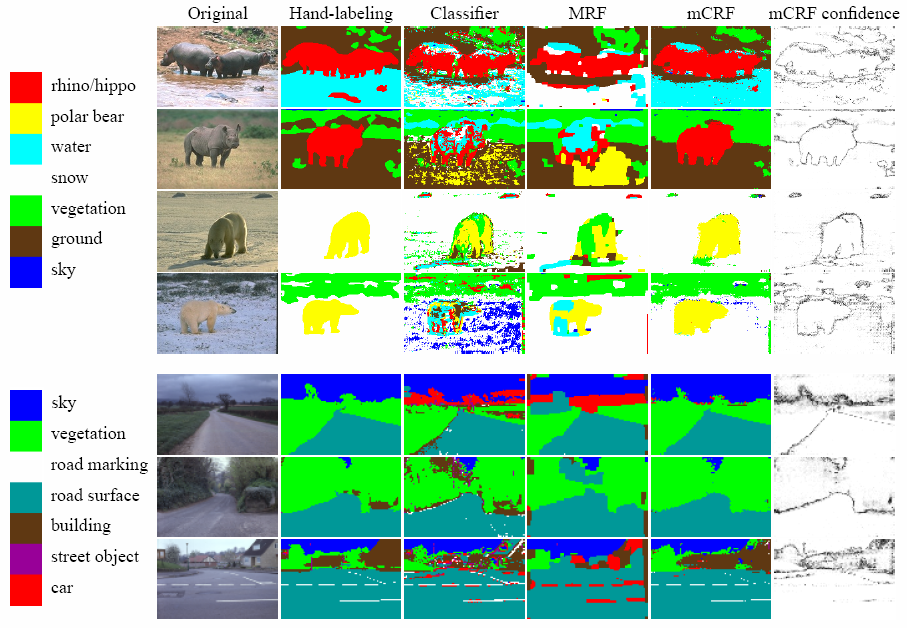
\includegraphics[width=1\columnwidth]{img-mCRF}

}

%%%%%%%%%%%%%%%%%%%%%%%%%%%%%%%%%%%%%%%%%%%%%%%%%%%%%%%%%%%%%%%%%%%%%%%%%%%%%%%%

\slide{CRFs in image processing}{

\item Google ``conditional random field image''

\begin{items}
\item Multiscale Conditional Random Fields for Image Labeling
(CVPR 2004)

\item Scale-Invariant Contour Completion Using Conditional Random Fields
(ICCV 2005)

\item Conditional Random Fields for Object Recognition (NIPS 2004)

\item Image Modeling using Tree Structured Conditional Random Fields
(IJCAI 2007)

\item A Conditional Random Field Model for Video Super-resolution
(ICPR 2006)
\end{items}

}

%%%%%%%%%%%%%%%%%%%%%%%%%%%%%%%%%%%%%%%%%%%%%%%%%%%%%%%%%%%%%%%%%%%%%%%%%%%%%%%%

%% \slide{From Regression to Structured Output}{

%% \item Our first step in regression was to define $f:~ \RRR^d\to\RRR$ as
%% $$f(x) = \phi(x)^\T \b$$
%% -- we defined a loss function\\
%% -- derived optimal parameters $\b$

%% ~

%% ~

%% \cen{How could we \textbf{represent} a discrete-valued function
%% $F:~ \RRR^d\to Y$?}

%% ~

%% ~\mypause

%% \cen{\Large\textbf{$\to$~ Discriminative Function}}

%% }

%%%%%%%%%%%%%%%%%%%%%%%%%%%%%%%%%%%%%%%%%%%%%%%%%%%%%%%%%%%%%%%%%%%%%%%%%%%%%%%%

\key{Conditional random fields**}
\slide{Conditional Random Fields (CRFs)}{

\item CRFs are a generalization of logistic binary and multi-class
classification

\item The output $y$ may be an arbitrary (usually discrete) thing
(e.g., sequence/image/graph-labelling)


\item Hopefully we can maximize efficiently
$$\argmax_y f(x,y)$$
over the output!

$\to$ $f(x,y)$ should be \emph{structured} in $y$ so this optimization
is efficient.

~

\item The name CRF describes that  $p(y | x)
 \propto e^{f(x,y)}$ defines a probability distribution (a.k.a.\
 random field) over the output $y$ conditional to the input $x$. The
 word ``field'' usually means that this distribution is structured (a
 graphical model; see later part of lecture).

}

%%%%%%%%%%%%%%%%%%%%%%%%%%%%%%%%%%%%%%%%%%%%%%%%%%%%%%%%%%%%%%%%%%%%%%%%%%%%%%%%

\slide{CRFs: the structure is in the features}{

\item Assume $y = (y_1,..,y_l)$ is a tuple of individual (local)
discrete labels

\item We can assume that $f(x,y)$ is linear in features
$$f(x,y) = \sum_{j=1}^k \phi_j(x,y_{\del j}) \b_j = \phi(x,y)^\T \b$$
where \textbf{each feature $\phi_j(x,y_{\del j})$ depends only on a
subset $y_{\del j}$ of labels}. $\phi_j(x,y_{\del j})$ effectively
couples the labels $y_{\del j}$. Then $e^{f(x,y)}$ is
a \textbf{factor graph}.

}

%%%%%%%%%%%%%%%%%%%%%%%%%%%%%%%%%%%%%%%%%%%%%%%%%%%%%%%%%%%%%%%%%%%%%%%%%%%%%%%%

\slide{Example: pair-wise coupled pixel labels}{

\show[.5]{mrf2}

\item Each black box corresponds to features $\phi_j(y_{\del j})$
which couple  neighboring pixel labels $y_{\del j}$

\item Each gray box corresponds to features $\phi_j(x_j,y_j)$ which
couple a local pixel observation $x_j$ with a pixel label $y_j$

}

%%%%%%%%%%%%%%%%%%%%%%%%%%%%%%%%%%%%%%%%%%%%%%%%%%%%%%%%%%%%%%%%%%%%%%%%%%%%%%%%

\slide{CRFs:~ Core equations}{

\vspace*{-5mm}
\begin{align*}
f(x,y)
 &= \phi(x,y)^\T \b \\
p(y | x)
 &= \frac{e^{f(x,y)}}{\sum_{y'} e^{f(x,y')}}
  = e^{f(x,y) - Z(x,\b)} \\
Z(x,\b)
 &= \log \sum_{y'} e^{f(x,y')} \quad\text{(log partition function)}\\
L(\b)
 &= - \sum_i \log p(y_i | x_i)
  = - \sum_i [f(x_i,y_i) - Z(x_i,\b)] \\
\na Z(x,\b)
 &= \sum_y p(y|x)~ \na f(x,y) \\
\he Z(x,\b)
 &= \sum_y p(y|x)~ \na f(x,y)~ \na f(x,y)^\T
  - \na Z~ \na Z^\T
\end{align*}

~

\item This gives the neg-log-likelihood $L(\b)$, its gradient and
Hessian

}

%%%%%%%%%%%%%%%%%%%%%%%%%%%%%%%%%%%%%%%%%%%%%%%%%%%%%%%%%%%%%%%%%%%%%%%%%%%%%%%%

\slide{Training CRFs}{\label{lastpage}

\item Maximize conditional likelihood

{\small
But Hessian is typically too large (Images: $\sim$10\,000
pixels, $\sim$50\,000 features)

If $f(x,y)$ has a chain structure over $y$, the Hessian is usually
banded $\to$ computation time linear in chain length

}

~

Alternative: Efficient gradient method, e.g.:

{\tiny Vishwanathan et al.: Accelerated Training of Conditional Random
Fields with Stochastic Gradient Methods

}

~

\item Other loss variants, e.g., hinge loss as with Support Vector Machines

{\tiny(``Structured output SVMs'')}

~

\item Perceptron algorithm: Minimizes hinge loss using a
gradient method

}

%%%%%%%%%%%%%%%%%%%%%%%%%%%%%%%%%%%%%%%%%%%%%%%%%%%%%%%%%%%%%%%%%%%%%%%%%%%%%%%%

%\slide{End of Part I: The Basis}{

%% \cen{\fbox{\begin{minipage}{.28\columnwidth}\center
%% \textbf{features/kernel}\\\tiny
%% polynomial\\
%% RBF\\
%% sigmoidal\\
%% kernel
%% \end{minipage}
%% &+&
%% \begin{minipage}{.28\columnwidth}\center
%% \textbf{regularization}\\{\tiny
%% Ridge\\
%% Lasso\\}
%% \textbf{cross validation}
%% \end{minipage}
%% &+&
%% \begin{minipage}{.28\columnwidth}\center
%% \textbf{loss}\\\tiny
%% least squares regression\\
%% likelihood maximization\\
%% (logistic regression)\\
%% (cond.\ random fields)
%% \end{minipage}}}

%% ~

%% ~

%% \item I consider this to be a core basis for understanding ML methods

%% \begin{itemize}
%% \item In terms of regression/classification performance, they should be
%% state-of-the-art (for good choice of features/kernel)

%% \item But in direct form these are not always computationally most
%% efficient
%% \end{itemize}

%% ~

%% \item \textbf{Part 2} will consider a multitude of ideas to extend this

%% ~

%% \item \textbf{Part 3} will introduce to the Bayesian formalism, which
%% allows to derive the same core methods from another prespective---and
%% extend them

%}

%% % \show[.4]{bigHammer}

%% ~

%% ~


%% \item Optimization in these methods can become computationally heavy (due
%% to matrix inversion scaling in $O(n^3)$).

%% Alternatives:

%% $\to$ (stochastic) gradient descent or other approximate optimization

%% $\to$ local/lazy methods: models around local neighborhood, using
%% nearest-neighbor smoothing kernels

%% $\to$ efficient alternatives like SVMs (Hinge loss)

%%%%%%%%%%%%%%%%%%%%%%%%%%%%%%%%%%%%%%%%%%%%%%%%%%%%%%%%%%%%%%%%%%%%%%%%%%%%%%%%

\slidesfoot

\providecommand{\slides}{
  \newcommand{\slideshead}{
  \newcommand{\thepage}{\arabic{mypage}}
  %beamer
%  \documentclass[t,hyperref={bookmarks=true}]{beamer}
%  \geometry{papersize={171mm,96mm}}
  \documentclass[t,hyperref={bookmarks=true},aspectratio=169]{beamer}
  \setbeamersize{text margin left=5mm}
  \setbeamersize{text margin right=5mm}
  \usetheme{default}
  \usefonttheme[onlymath]{serif}
  \setbeamertemplate{navigation symbols}{}
  \setbeamertemplate{itemize items}{{\color{black}$\bullet$}}

  \newwrite\keyfile

  %\usepackage{palatino}
  \stdpackages
  %\usepackage{tikz} \usetikzlibrary {shapes.geometric} 
  \usepackage{multimedia}
  \usepackage[utf8]{inputenc}

  %%% geometry/spacing issues
  %
  \definecolor{bluecol}{rgb}{0,0,.5}
  \definecolor{greencol}{rgb}{0,.6,0}
  \definecolor{citcol}{rgb}{.4,.4,.4}
  %\renewcommand{\baselinestretch}{1.1}
  \renewcommand{\arraystretch}{1.2}
  \columnsep 0mm

  \columnseprule 0pt
  \parindent 0ex
  \parskip 0ex
  %\setlength{\itemparsep}{3ex}
  %\renewcommand{\labelitemi}{\rule[3pt]{10pt}{10pt}~}
  %\renewcommand{\labelenumi}{\textbf{(\arabic{enumi})}}
  \setbeamertemplate{enumerate item}{(\roman{enumi})}
  \newcommand{\headerfont}{\helvetica{14}{1.5}{b}{n}}
  \newcommand{\slidefont} {\helvetica{11}{1.4}{m}{n}}
  %\newcommand{\codefont} {\helvetica{8}{1.2}{m}{n}}
  \renewcommand{\small} {\helvetica{10}{1.4}{m}{n}}
  \renewcommand{\tiny} {\helvetica{8}{1.3}{m}{n}}
  \newcommand{\ttiny} {\helvetica{7}{1.3}{m}{n}}

  %%% count pages properly and put the page number in bottom right
  %
  \newcounter{mypage}
  \newcommand{\incpage}{\addtocounter{mypage}{1}\setcounter{page}{\arabic{mypage}}}
  \setcounter{mypage}{0}
  \resetcounteronoverlays{page}

  \pagestyle{fancy}
  %\setlength{\headsep}{10mm}
  %\addtolength{\footheight}{15mm}
  \renewcommand{\headrulewidth}{0pt} %1pt}
  \renewcommand{\footrulewidth}{0pt} %.5pt}
  \cfoot{}
  \rhead{}
  \lhead{}
  %% \lfoot{\vspace*{-3mm}\hspace*{-3mm}\helvetica{5}{1.3}{m}{n}{\texttt{github.com/MarcToussaint/AI-lectures}}}
\lfoot{}
%  \rfoot{{\tiny\textsf{AI -- \topic -- \subtopic -- \arabic{mypage}/\pageref{lastpage}}}}
  %\lfoot{\raisebox{5mm}{\tiny\textsf{\slideauthor}}}
  %\rfoot{\raisebox{5mm}{\tiny\textsf{\slidevenue{} -- \arabic{mypage}/\pageref{lastpage}}}}
  %\rfoot{~\anchor{30,12}{\tiny\textsf{\thepage/\pageref{lastpage}}}}
  %\lfoot{\small\textsf{Marc Toussaint}}
  \rfoot{\vspace*{-4.5mm}{\tiny\textsf{\color{gray}\topic\ -- \subtopic\ -- \arabic{mypage}/\pageref{lastpage}}}\hspace*{-4mm}}
%  \rfoot{~\anchor{-10,12}{\tiny\textsf{\color{gray}\topic\ --  \arabic{mypage}/\pageref{lastpage}}}}
  \lfoot{\vspace*{-4.5mm}{\hspace*{-3mm}\includegraphics[height=4mm]{LIS-logo-longText}}}

  \definecolor{grey}{rgb}{.8,.8,.8}
  \definecolor{head}{rgb}{.85,.9,.9}
%  \definecolor{blue}{rgb}{.0,.0,.5}
%  \definecolor{green}{rgb}{.0,.5,.0}
  \definecolor{red}{rgb}{.8,.0,.0}
  \newcommand{\inverted}{
    \definecolor{main}{rgb}{1,1,1}
    \color{main}
    \pagecolor[rgb]{.3,.3,.3}
  }
  \input{../latex/macros}

  \graphicspath{{pics/}{../pics/}{../latex/pics/}}
}

\newcommand{\lecturetitleslide}{
  \title{\course \topic}
  \author{Marc Toussaint}
  \institute{Learning \& Intelligent Systems Lab, TU Berlin}

  \begin{document}


  %% title slide!
  \slide{}{
    \thispagestyle{empty}

    \twocol{.27}{.6}{
      %\vspace*{-5mm}%
      \hspace*{-5mm}%
      \includegraphics[width=1.\columnwidth]{\coursepicture}
    }{\center

      \textbf{\fontsize{17}{20}\selectfont \course}

      ~

      %Lecture
      \topic\\

      \vspace{1cm}

      {\tiny~\emph{\keywords}~\\}

      \vspace{1cm}

      Marc Toussaint
      
      Technical University of Berlin

      \coursedate

      ~

    }
  }
}

\newcommand{\slide}[2]{
  \slidefont
  \incpage\begin{frame}
  \addcontentsline{toc}{section}{#1}
  \vfill
  {\headerfont #1} \vspace*{-2ex}
  \begin{itemize}\item[]~\\
    #2
  \end{itemize}
  \vfill
  \end{frame}
}

% use \begin{frame}[fragile] around slidecore!
\newenvironment{slidecore}[1]{
  \slidefont\incpage
  \addcontentsline{toc}{section}{#1}
  \vfill
  {\headerfont #1} \vspace*{-2ex}
  \begin{itemize}\item[]~\\
}{
  \end{itemize}
  \vfill
}

\newcommand{\titleslide}[4][Marc Toussaint]{
  \newcommand{\slideauthor}{#1}
  \newcommand{\slidevenue}{#3}
  \slidefont
  \incpage
  \begin{frame}
  \begin{center}
    \vspace*{15mm}

    {\headerfont #2\\}
        
    \vspace*{10mm}

    #1 \\

    \vspace*{5mm}

    {\small
      Learning \& Intelligent Systems Lab, TU Berlin\\
%      Science of Intelligence Cluster of Excellence, Berlin\\
      Max Planck Fellow, Institute for Intelligent Systems\\ %Physical Reasoning \& Manipulation Lab -- 
%      MIT CSAIL\\
%      mtoussai@mit.edu,~ marc.toussaint@informatik.uni-stuttgart.de

      \vspace*{10mm}

      \emph{#3}
    }

    \vspace*{0mm}

    %\includegraphics[scale=.1]{pics/eushield-fullcolour}

  \end{center}
  \begin{itemize}\item[]~\\
    #4
  \end{itemize}
  \end{frame}
}

\newcommand{\titleslideempty}[2]{
  \slidefont
  \incpage
  \begin{frame}
  \begin{center}
    \vspace*{15mm}

    {\headerfont #1\\}
        
    %% \vspace*{5mm}

    %% {\small\emph{#2}} \\

  \end{center}
  \begin{itemize}\item[]~\\
    #2
  \end{itemize}
  \end{frame}
}

\providecommand{\key}[1]{
  \addtocounter{mypage}{1}
% \immediate\write\keyfile{#1}
  \addtocontents{toc}{\hyperref[key:#1]{#1 (\arabic{mypage})}}
%  \phantomsection\label{key:#1}
%  \index{#1@{\hyperref[key:#1]{#1 (\arabic{mysec}:\arabic{mypage})}}|phantom}
  \addtocounter{mypage}{-1}
}

\providecommand{\course}{}

\providecommand{\subtopic}{}

\providecommand{\sublecture}[2]{
  \renewcommand{\subtopic}{#1}
  \slide{#1}{#2}
}

\providecommand{\sublectureHide}[2]{
  \renewcommand{\subtopic}{#1}
}

\providecommand{\story}[1]{
~

Motivation: {\tiny #1}\clearpage
}

\newenvironment{items}[1][9]{
\par\setlength{\unitlength}{1pt}\fontsize{#1}{#1}\linespread{1.2}\selectfont
\begin{list}{--}{\leftmargin4ex \rightmargin0ex \labelsep1ex \labelwidth2ex
\topsep0pt \parsep0ex \itemsep3pt}
}{
\end{list}
}

\newenvironment{itemS}[1][4ex]{
\par
\tiny
\begin{list}{--}{\leftmargin#1 \rightmargin0ex \labelsep1ex
  \labelwidth2ex \topsep0pt \parsep0ex \itemsep2pt}
}{
\end{list}
}

\providecommand{\slidesfoot}{
  \end{document}
}


  \slideshead
  \lecturetitleslide
}

\providecommand{\exercises}{
  \newcommand{\exerciseshead}{
  \documentclass[10pt,fleqn]{article}
  \stdpackages
\usepackage[utf8]{inputenc}

  \definecolor{bluecol}{rgb}{0,0,.5}
  \definecolor{greencol}{rgb}{0,.4,0}
  \definecolor{shadecolor}{gray}{0.9}
  \usepackage[
    %    pdftex%,
    %%    letterpaper,
    %    bookmarks,
    %    bookmarksnumbered,
    colorlinks,
    urlcolor=bluecol,
    citecolor=black,
    linkcolor=bluecol,
    %    pagecolor=bluecol,
    pdfborder={0 0 0},
    %pdfborderstyle={/S/U/W 1},
    %%    backref,     %link from bibliography back to sections
    %%    pagebackref, %link from bibliography back to pages
    %%    pdfstartview=FitH, %fitwidth instead of fit window
    pdfpagemode=UseNone, %UseOutlines, %bookmarks are displayed by acrobat
    pdftitle={\course},
    pdfauthor={Marc Toussaint},
    pdfkeywords={}
  ]{hyperref}
  \DeclareGraphicsExtensions{.pdf,.png,.jpg,.eps}

  \renewcommand{\r}{\varrho}
  \renewcommand{\l}{\lambda}
  \renewcommand{\L}{\Lambda}
  \renewcommand{\b}{\beta}
  \renewcommand{\d}{\delta}
  \renewcommand{\k}{\kappa}
  \renewcommand{\t}{\theta}
  \renewcommand{\O}{\Omega}
  \renewcommand{\o}{\omega}
  \renewcommand{\SS}{{\cal S}}
  \renewcommand{\=}{\!=\!}
  %\renewcommand{\boldsymbol}{}
  %\renewcommand{\Chapter}{\chapter}
  %\renewcommand{\Subsection}{\subsection}

  \renewcommand{\baselinestretch}{1.1}
  \geometry{a4paper,headsep=7mm,hdivide={15mm,*,15mm},vdivide={20mm,*,15mm}}

  \fancyhead[L]{\thetitle, \textit{\teacher}---\coursedate}
  \fancyhead[R]{\thepage}
  \fancyhead[C]{}
  \fancyfoot{}
  \pagestyle{fancy}

  \renewcommand{\labelenumi}{{\alph{enumi})}}

  \parindent 0pt
  \parskip 0.5ex

  \newcommand{\codefont}{\helvetica{8}{1.2}{m}{n}}

  \input{../latex/macros}

  \DefineShortVerb{\@}

  \usepackage{comment}
  \specialcomment{solution}{
    \small
    \begin{shaded}
  }{
    \end{shaded}
  }
  
  \renewcommand{\hat}{\widehat}
  \newcommand{\bbg}{{\bar{\bar g}}}
  \graphicspath{{pics/}{../latex/pics/}}

  \mytitle{\course\\\exnum}
  \myauthor{\teacher\\ \small\addressTUB}
  \date{\coursedate}
}

  %%%%%%%%%%%%%%%%%%%%%%%%%%%%%%%%%%%%%%%%%%%%%%%%%%%%%%%%%%%%%%%%%%%%%%%%%%%%%%%%

\newcommand{\exercisestitle}{  
  \begin{document}
  \maketitle
}

\newcommand{\exsection}[1]{\section{#1}}

\newcommand{\exerfoot}{
  \end{document}
}

\newenvironment{items}[1][9]{
  \par\setlength{\unitlength}{1pt}\fontsize{#1}{#1}\linespread{1.2}\selectfont
  \begin{list}{--}{\leftmargin4ex \rightmargin0ex \labelsep1ex \labelwidth2ex
      \topsep0pt \parsep0ex \itemsep3pt}
}{
  \end{list}
}

  \exerciseshead
}

\providecommand{\script}{
  \newcommand{\scripthead}{
  \documentclass[9pt,fleqn,twoside]{article}
  \stdpackages

  \usepackage{makeidx}
  \makeindex

  \usepackage{thmtools}
  \definecolor{shadecolor}{gray}{0.85}
  \declaretheoremstyle[
    %headfont=\normalfont\bfseries,
    %notefont=\mdseries, notebraces={(}{)},
    %bodyfont=\normalfont,
    %postheadspace=0.5em,
    %spaceabove=6pt,
    mdframed={
      %  skipabove=8pt,
      %  skipbelow=6pt,
      hidealllines=true,
      backgroundcolor={shadecolor},
      innertopmargin=8pt,
      %  innerleftmargin=3pt,
      %  innerrightmargin=3pt
    }
  ]{shaded}
  \declaretheorem[style=shaded,within=section,name=Definition]{myDefinition}
  \declaretheorem[style=shaded,within=section,name=Theorem]{myTheorem}
  \declaretheorem[style=shaded,within=section,name=Identities]{Identities}
  \declaretheorem[style=shaded,within=section,name=Example]{myExample}

  \definecolor{grey}{rgb}{.8,.8,.8}
  \definecolor{bluecol}{rgb}{0,0,.5}
  \definecolor{greencol}{rgb}{0,.4,0}
  \definecolor{shadecolor}{gray}{0.9}
  \definecolor{citcol}{rgb}{.4,.4,.4}
  \usepackage[
    %    pdftex%,
    %%    letterpaper,
    %bookmarks,
    bookmarksnumbered,
    colorlinks,
    urlcolor=bluecol,
    citecolor=black,
    linkcolor=bluecol,
    %    pagecolor=bluecol,
    pdfborder={0 0 0},
    %pdfborderstyle={/S/U/W 1},
    %%    backref,     %link from bibliography back to sections
    %%    pagebackref, %link from bibliography back to pages
    %%    pdfstartview=FitH, %fitwidth instead of fit window
    pdfpagemode=UseOutlines, %bookmarks are displayed by acrobat
    pdftitle={\course},
    pdfauthor={Marc Toussaint},
    pdfkeywords={}
  ]{hyperref}
  \DeclareGraphicsExtensions{.pdf,.png,.jpg,.eps}

  %\usepackage{multirow}
  \usepackage{multimedia}
  %\usepackage{marginnote}
  %\setbeamercolor{background canvas}{bg=}

  \usepackage[round]{natbib}
  \bibliographystyle{abbrvnat}

  \renewcommand{\r}{\varrho}
  \renewcommand{\l}{\lambda}
  \renewcommand{\L}{\Lambda}
  \renewcommand{\b}{\beta}
  \renewcommand{\d}{\delta}
  \renewcommand{\k}{\kappa}
  \renewcommand{\t}{\theta}
  \renewcommand{\O}{\Omega}
  \renewcommand{\o}{\omega}
  \renewcommand{\SS}{{\cal S}}
  \renewcommand{\=}{\!=\!}
  %\renewcommand{\boldsymbol}{}
  %\renewcommand{\Chapter}{\chapter}
  %\renewcommand{\Subsection}{\subsection}

  \renewcommand{\baselinestretch}{1.0}
  \geometry{a5paper,headsep=6mm,hdivide={10mm,*,10mm},vdivide={13mm,*,7mm}}

  \fancyhead[OL,ER]{\course, \textit{Marc Toussaint}}
  \fancyhead[OR,EL]{\thepage}
  \fancyhead[C]{}
  \fancyfoot{}
  \pagestyle{fancy}

  \renewcommand{\labelenumi}{{(\roman{enumi})}}
  \renewcommand{\theenumi}{(\roman{enumi})} %for ref
  \parindent 0pt
  \parskip .5pc

  \columnsep 6ex

  \renewcommand{\familydefault}{\sfdefault}

  \newcommand{\headerfont}{\large}%helvetica{12}{1}{b}{n}}
  \newcommand{\slidefont} {}%\helvetica{9}{1.3}{m}{n}}
  \newcommand{\storyfont} {}
  %  \renewcommand{\small}   {\helvetica{8}{1.2}{m}{n}}
  \renewcommand{\tiny}    {\footnotesize}%helvetica{7}{1.1}{m}{n}}
  \newcommand{\ttiny} {\footnotesize}%fontsize{7}{7}\selectfont}
%  \newcommand{\codefont}{\fontsize{6}{6}\selectfont}%helvetica{8}{1.2}{m}{n}}
  \newcommand{\codefont} {\helvetica{8}{1.2}{m}{n}}

  \input{../latex/macros}

  \usepackage{comment}
  \specialcomment{solution}{
    \small
    \begin{shaded}
  }{
    \end{shaded}
  }

  \graphicspath{{pics/}{../pics/}{pics-local/}}

  \mytitle{\course\\Lecture Script}
  \myauthor{Marc Toussaint}
  \date{\coursedate}
}

%%%%%%%%%%%%%%%%%%%%%%%%%%%%%%%%%%%%%%%%%%%%%%%%%%%%%%%%%%%%%%%%%%%%%%%%%%%%%%%%

\newcommand{\scripttitle}{
  \begin{document}
  \maketitle
  %\anchor{100,10}{\includegraphics[width=4cm]{optim}}
%  \vspace*{1cm}
}

%%%%%%%%%%%%%%%%%%%%%%%%%%%%%%%%%%%%%%%%%%%%%%%%%%%%%%%%%%%%%%%%%%%%%%%%%%%%%%%%

\newcounter{mypage}
\setcounter{mypage}{0}
\newcommand{\incpage}{\addtocounter{mypage}{1}}

\newcommand{\subtopic}{}
\newcommand{\pause}{}
\newcommand{\only}[1]{#1}

\renewcommand{\slides}[1][]{
  %  \clearpage
  \subsection{\topic}
  \index{\topic}
  {\small #1}
  \setcounter{mypage}{0}
  \smallskip\nopagebreak\hrule\medskip
}

\newcommand{\slidesfoot}{
  \bigskip
}

\newcommand{\sublecture}[2]{
  \phantomsection\addcontentsline{toc}{subsubsection}{#1}
  \index{#1}
}

\newcommand{\sublectureHide}[2]{
  \renewcommand{\subtopic}{#1}
}

\newcommand{\key}[1]{
  \phantomsection\addcontentsline{toc}{subsubsection}{#1}
  %\subsubsection{#1}
  \index{#1}
}

\providecommand{\defn}[1]{%
  \textbf{#1}\index{#1}%
}

\newenvironment{slidecore}[1]{
  \incpage
  \subsubsection*{#1}%{\headerfont\noindent\textbf{#1}\\}%
  \vspace{-6ex}%
  \begin{list}{$\bullet$}{\leftmargin4ex \rightmargin0ex \labelsep1ex
    \labelwidth2ex \partopsep0ex \topsep0ex \parsep.5ex \parskip0ex \itemsep0pt}\item[]~\\\nopagebreak%
}{
  \end{list}\nopagebreak%
  {\hfill\tiny \textsf{\arabic{section}.\arabic{subsection}:\arabic{mypage}}}\nopagebreak%
  \smallskip\nopagebreak\hrule
}

\newcommand{\slide}[2]{
  \begin{slidecore}{#1}
    #2
  \end{slidecore}
}

\renewcommand{\exercises}{}
\newcommand{\exercisestitle}{}
\newcommand{\exsection}[1]{\subsubsection{#1}}
\newcommand{\exsubsection}[1]{\paragraph{#1}}
\newcommand{\exerfoot}{\bigskip}

\newcommand{\story}[1]{
  \subsection*{Motivation \& Outline}
  {\storyfont\sf #1}
  \medskip\nopagebreak\hrule
}

\newcounter{savedsection}
\newcommand{\subappendix}{\setcounter{savedsection}{\arabic{section}}\appendix}
\newcommand{\noappendix}{
  \setcounter{section}{\arabic{savedsection}}% restore section number
  \setcounter{subsection}{0}% reset section counter
%  \gdef\@chapapp{\sectionname}% reset section name
  \renewcommand{\thesection}{\arabic{section}}% make section numbers arabic
}

\newenvironment{items}[1][9]{
\par\setlength{\unitlength}{1pt}\fontsize{#1}{#1}\linespread{1.2}\selectfont
\begin{list}{--}{\leftmargin4ex \rightmargin0ex \labelsep1ex \labelwidth2ex
\topsep0pt \parsep0ex \itemsep3pt}
}{
\end{list}
}

\newenvironment{itemS}[1][4ex]{
\par
\tiny
\begin{list}{--}{\leftmargin#1 \rightmargin0ex \labelsep1ex
  \labelwidth2ex \topsep0pt \parsep0ex \itemsep2pt}
}{
\end{list}
}

\newcommand{\Def}[1]{%
\textbf{#1}\index{#1}}%\marginnote{#1}}

  \scripthead
}

\providecommand{\paper}{
  \input{../latex/style-paper}
  \paperhead
}

\providecommand{\note}{
  \providecommand{\notehead}[2]{
  \documentclass[#1,fleqn,twoside]{article}
  \stdpackages
  \renewcommand{\labelenumi}{{(\roman{enumi})}}
  \renewcommand{\theenumi}{(\roman{enumi})} %for ref

  \renewcommand{\baselinestretch}{#2}
  \renewcommand{\arraystretch}{1.2}
  \renewcommand{\topfraction}{1}
  \renewcommand{\bottomfraction}{1}
  \renewcommand{\textfraction}{0}
  \columnsep 5ex
  \parindent 3ex
  \parskip 1ex

  % Lists and paragraphs
  \parindent 0pt
  \topsep 4pt plus 1pt minus 2pt
  \partopsep 1pt plus 0.5pt minus 0.5pt
  \itemsep 2pt plus 1pt minus 0.5pt
  \parsep 2pt plus 1pt minus 0.5pt
  \parskip .5pc %add _in_ {thebibliography} environment in *.bbl

  \setcounter{tocdepth}{3}
  \setcounter{secnumdepth}{3}

  \geometry{a4paper,hdivide={25mm,*,25mm},vdivide={25mm,*,25mm}}

  \renewcommand{\headrulewidth}{.0pt}\renewcommand{\footrulewidth}{.0pt}\cfoot{}
  \fancyhead[OL,EC]{\it\theauthor---\today}
  \fancyhead[ER]{\leftmark}
  \fancyhead[OR,EL]{\thepage}
  \fancyfoot[EL,OR]{}
  \setlength{\headsep}{10mm}
  %\fancyhead[OL]{\rightmark}
  %\fancyfoot[EL,OR]{}


  %  \usepackage{palatino}

  \newcommand{\codefont}{\helvetica{8}{1.2}{m}{n}}

  \renewenvironment{abstract}{
    \vspace*{5ex}\begin{list}{}{
      \leftmargin3ex
      \rightmargin3ex
      \topsep-\parskip}\item[]
     \hrule\vspace{1.5ex}{\bf Abstract.~}\small}
    {\vspace{2ex}\hrule\end{list}\vspace{5ex}}
    
  \newenvironment{keyword}
    {\par{\it Keywords:~}}
    {}

  \def\makemytitle{%
    \thispagestyle{empty}
    \begin{list}{}{\leftmargin3ex \rightmargin3ex \topsep0ex \parsep0ex}\item[]
      \begin{center}
        {\fontsize{18}{25}\selectfont{\thetitle\\}}\vspace{5ex}

        {\fontsize{14}{16}\selectfont{\theauthor\\}}\vspace{1ex}

        {\footnotesize{\sl \addressFUB}\\ \emailBerlin}

        {\footnotesize \today}

        \vspace{1ex}
        {\small \published}
      \end{center}
    \end{list}
    \renewcommand{\maketitle}{\chapter{\thetitle}}
  }

  \input{../latex/macros}
  \pdflatex

  \graphicspath{{pics/}{../pics/}{pics-local/}}

  \myauthor{Marc Toussaint}
  \date{\today}
}

%%%%%%%%%%%%%%%%%%%%%%%%%%%%%%%%%%%%%%%%%%%%%%%%%%%%%%%%%%%%%%%%%%%%%%%%%%%%%%%%

\newcommand{\notetitle}{
  \begin{document}
  \thispagestyle{empty}
    
  \maketitle

}

\newenvironment{items}[1][9]{
\par\setlength{\unitlength}{1pt}\fontsize{#1}{#1}\linespread{1.2}\selectfont
\begin{list}{--}{\leftmargin4ex \rightmargin0ex \labelsep1ex \labelwidth2ex
\topsep0pt \parsep0ex \itemsep3pt}
}{
\end{list}
}

  \notehead{10}{1.1}
}

\providecommand{\course}{NO COURSE}
\providecommand{\coursepicture}{NO PICTURE}
\providecommand{\coursedate}{NO DATE}
\providecommand{\topic}{NO TOPIC}
\providecommand{\keywords}{NO KEYWORDS}
\providecommand{\exnum}{NO NUMBER}
\providecommand{\teacher}{Marc Toussaint}

\providecommand{\stdpackages}{
  \usepackage{amsmath}
  \usepackage{amssymb}
  \usepackage{amsfonts}
  \allowdisplaybreaks
  \usepackage{amsthm}
  \usepackage{eucal}
  \usepackage{graphicx}
%  \usepackage{color}
  \usepackage{geometry}
  \usepackage{framed}
  \usepackage{xcolor}
  \definecolor{shadecolor}{gray}{0.9}
  \setlength{\FrameSep}{3pt}
  \usepackage{fancyvrb}
  \fvset{numbers=none,xleftmargin=5ex,fontsize=\small}

  \usepackage{pdfpages}

  \usepackage{multicol} 
  \usepackage{fancyhdr}
}

\providecommand{\addressUSTT}{
  Machine~Learning~\&~Robotics~lab, U~Stuttgart\\\small
  Universit{\"a}tsstra{\ss}e 38, 70569~Stuttgart, Germany
}

\providecommand{\addressTUB}{
  Learning~\&~Intelligent~Systems~Lab, TU~Berlin\\\small
  Marchstr. 23, 10587 Berlin, Germany
}


\renewcommand{\course}{Machine Learning}
\renewcommand{\coursepicture}{course_ml}
\renewcommand{\coursedate}{Summer 2019}
\renewcommand{\topic}{Neural Networks}
\renewcommand{\keywords}{NN models, objectives \& regularization,
training, stochastic gradient descent, computation graphs, images \& sequences, architectures}

\slides

%%%%%%%%%%%%%%%%%%%%%%%%%%%%%%%%%%%%%%%%%%%%%%%%%%%%%%%%%%%%%%%%%%%%%%%%%%%%%%%%

\slide{Outline}{

\item Model, Objective, Solver:
\begin{items}
\item How do NNs represent a function $f(x)$, or discriminative function $f(y,x)$?

\item What are objectives? ~ (standard objectives, different regularizations)

\item How are they trained? ~ (Initialization, SGD)
\end{items}

\item Computation Graphs \& Chain Rules

\item Images \& Sequences
\begin{items}
\item CNNs
\item LSTMs \& GRUs
\item Complex architectures ~ (e.g.\ Mask-RCNN, dense pose prediction, etc)
\end{items}


}

%%%%%%%%%%%%%%%%%%%%%%%%%%%%%%%%%%%%%%%%%%%%%%%%%%%%%%%%%%%%%%%%%%%%%%%%%%%%%%%%

\slide{Neural Network models}{

\item NNs are a parameterized function $f_\b: \RRR^d \mapsto \RRR^M$
\begin{items}
\item $\beta$ are called weights
\item Given a data set $D=\{(x_i,y_i)\}_{i=1}^n$, we minimize some loss
$$\beta^* = \argmin_\b \sum_{i=1}^n \ell(f_\b(x_i), y_i) + \text{~regularization}$$
\end{items}

\item In that sense, they just replace our previous model assumption $f(x) = \phi(x)^\T \b$, the reset is ``in principle'' the same

}

%%%%%%%%%%%%%%%%%%%%%%%%%%%%%%%%%%%%%%%%%%%%%%%%%%%%%%%%%%%%%%%%%%%%%%%%%%%%%%%%

\key{Neural Network function class}
\slide{Neural Network models}{

\item A (fwd-forward) NN $\RRR^{h_0} \mapsto \RRR^{h_L}$ with $L$ layers, each $h_l$-dimensional, defines the function
\begin{tabular}{l@{~}l@{~}l}
1-layer: & $f_\b(x) = W_1 x + b_1$, & $W_1 \in \RRR^{h_1\times h_0}, b_1\in\RRR^{h_1}$ \\
2-layer: & $f_\b(x) = W_2 \s(W_1 x+b_1) + b_2$, & $W_l \in \RRR^{h_l\times h_{l\1}}, b_l\in\RRR^{h_l}$ \\
$L$-layer: & $f_\b(x) = W_L \s(\cdots \s(W_1 x+b_1) \cdots) + b_L$\hspace*{-5mm}
\end{tabular}

\item The parameter $\b=(W_{1:L}, b_{1:L})$ is the collection of all\\
\textbf{weights} $W_l \in \RRR^{h_l\times h_{l\1}}$ and \textbf{biases} $b_l\in\RRR^{h_l}$

\item To describe the mapping as an iteration, we introduce notation for the intermediate values:
\begin{items}
\item the \textbf{input} to layer $l$ is $z_l = W_l x_{l\1} + b_l \in \RRR^{h_l}$
\item the \textbf{activation} of layer $l$ is $x_l = \s(z_l) \in \RRR^{h_l}$
\end{items}

Then the $L$-layer NN model can be computed using the \textbf{forward propagation:} 
$$\forall_{l=1,..,L\1}:~ z_l = W_l x_{l\1} + b_l \comma x_l=\s(z_l)$$
where $x_0\equiv x$ is the input, and $f_\b(x) \equiv z_L$ the output

}

%%%%%%%%%%%%%%%%%%%%%%%%%%%%%%%%%%%%%%%%%%%%%%%%%%%%%%%%%%%%%%%%%%%%%%%%%%%%%%%%

\slide{Neural Network models}{

\item The \textbf{activation function} $\s(z)$ is applied \emph{element-wise},

{\small
\begin{tabular}{ll}
rectified linear unit (ReLU) & $\s(z) = [z]_+ = \max\{0,z\} = z [z\ge 0]$\\
leaky ReLU & $\s(z) = \max\{0.01z, z\} =  \begin{cases} 0.01 z & z<0 \\ z & z\ge 0\end{cases}$\\
sigmoid, logistic & $\s(z) = 1/(1+e^{-z})$ \\
tanh & $\s(z) = \tanh(z)$
\end{tabular}
}

~

\item $L$-layer means $L-1$ hidden layers plus 1 output layer. (The input $x_0$ is not counted.)

~

\item The forward propagation therefore iterates applying
\begin{items}
\item a linear transformation $x_{l\1}\mapsto z_l$, highly parameterized with $W_l,b_l$
\item a non-linear transformation $z_l\mapsto x_l$, element-wise and without parameters
\end{items}

}

%%%%%%%%%%%%%%%%%%%%%%%%%%%%%%%%%%%%%%%%%%%%%%%%%%%%%%%%%%%%%%%%%%%%%%%%%%%%%%%%

\slide{}{

\only<1>{\show{NeuralNet-new-regression}}
\only<2>{\show{NeuralNet-new-classification}}
\only<3>{\show{NeuralNet-new-NN}}

}

%%%%%%%%%%%%%%%%%%%%%%%%%%%%%%%%%%%%%%%%%%%%%%%%%%%%%%%%%%%%%%%%%%%%%%%%%%%%%%%%

\slide{Neural Network models}{

\item We can think of the second-to-last layer $x_{L\1}$ as a feature vector

$$\phi_\b(x) = x_{L\1}$$

\item This aligns NNs models with what we discussed so far. But the crucial difference is:

\cen{\textbf{In NNs, the features $\phi_\b(x)$ are also parameterized and trained!}}

While in previous lectures, we had to fix $\phi(x)$ by hand, NNs allow us to learn features and \textbf{intermediate representations}

~\tiny

\item Note: It is a common approach to train NNs as usual, but after training fix the trained features $\phi(x)$ (``remove the head (=output layer) and fix the remaining body of the NN'') and use these trained features for similar problems or other kinds of ML on top.

}

%%%%%%%%%%%%%%%%%%%%%%%%%%%%%%%%%%%%%%%%%%%%%%%%%%%%%%%%%%%%%%%%%%%%%%%%%%%%%%%%

\slide{NNs as unversal function approximators}{

\item A 1-layer NN is linear in the input

\item Already a 2-layer NN with $h_1\to \infty$ hidden neurons is a universal function approximator
\begin{items}
\item Corresponds to $k\to\infty$ features $\phi(x)\in\RRR^k$ that are well tuned
\end{items}

}

%%%%%%%%%%%%%%%%%%%%%%%%%%%%%%%%%%%%%%%%%%%%%%%%%%%%%%%%%%%%%%%%%%%%%%%%%%%%%%%%

\slide{Objectives to train NNs}{

\begin{items}
\item loss functions
\item regularization
\end{items}

}

%%%%%%%%%%%%%%%%%%%%%%%%%%%%%%%%%%%%%%%%%%%%%%%%%%%%%%%%%%%%%%%%%%%%%%%%%%%%%%%%

\key{NN loss functions}
\slide{Loss functions as usual}{

\item Squared error regression, for $h_L$-dimensional output:
\begin{items}
\item for a single data point $(x,y^*)$, $\ell(f(x),y^*) = (f(x) - y^*)^2$

\item the loss gradient is $\frac{\del\ell}{\del f} = 2 (f-y^*)^\T$
\end{items}

~

\item For multi-class classification we have $h_L=M$ outputs, and $f_\beta(x)\in\RRR^M$ represents the discriminative function

\item Neg-log-likelihood or cross entropy loss:
\begin{items}
\item for a single data point $(x,y^*)$, $\ell(f(x),y^*) = -\log p(y^* | x)$

\item the loss gradient at output $y$ is $\frac{\del\ell}{\del f_y} = p(y|x) - [y=y^*]$
\end{items}

\item One-vs-all hinge loss:
\begin{items}
\item for a single data point $(x,y^*)$, $\ell(f(x),y^*) = \sum_{y\not=y^*} [1 - (f_{y^*}-f_y)]_+$,

\item the loss gradient at non-target outputs $y\not=y^*$ is $\frac{\del\ell}{\del f_y} = [f_{y^*} < f_y+1 ]$

\item the loss gradient at the target output $y^*$ is $\frac{\del\ell}{\del f_{y^*}} = -\sum_{y\not=y^*} [f_{y^*} < f_y+1]$
\end{items}

}

%%%%%%%%%%%%%%%%%%%%%%%%%%%%%%%%%%%%%%%%%%%%%%%%%%%%%%%%%%%%%%%%%%%%%%%%%%%%%%%%

\key{NN regularization}
\key{NN Dropout}
\slide{New types of regularization}{

\item Conventional, add a $L_2$ or $L_1$ regularization.
\begin{items}
\item adds a penalty $\l W_{l,ij}^2$ (Ridge) or $\l|W_{l,ij}|$ (Lasso) for every weight
\item In practise, compute the unregularized gradient as usual, then add $\l W_{l,ij}$ (for $L_2$),
or $\l\sign{W_{l,ij}}$ (for $L_1$) to the gradient
\item Historically, this is called \textbf{weight decay}, as the additional gradient (executed after the unregularized weight update) just decays weights
\end{items}

\item Dropout
\begin{items}
\item \emph{Srivastava et al: Dropout: a simple way to prevent neural networks from overfitting, JMLR 2014.}
\item ``a way  of  approximately  combining  exponentially  many  different  neural  network architectures efficiently''
\item ``$p$ can  simply  be  set  at  0.5,  which  seems  to  be  close  to  optimal  for  a  wide  range  ofnetworks and tasks''
\item on test/prediction time, take true averages
\end{items}


\item Others:
\begin{items}
\item Data Augmentation
\item Training ensembles, bagging (averaging bootstrapped models)
\item Additional embedding objectives (e.g.\ semi-supervised embedding)
\item Early stopping
\end{items}

}

%%%%%%%%%%%%%%%%%%%%%%%%%%%%%%%%%%%%%%%%%%%%%%%%%%%%%%%%%%%%%%%%%%%%%%%%%%%%%%%%

\key{data augmentation}
\slide{Data Augmentation}{

\item A very interesting form of regularization is to modify the data!

\item Generate more data by applying invariances to the given data. The model then learns to generalize as described by these invariances.

\item This is a form of regularization that directly incorporates expert knowledge

~

\show[.6]{dataAugmentation}

}

%%%%%%%%%%%%%%%%%%%%%%%%%%%%%%%%%%%%%%%%%%%%%%%%%%%%%%%%%%%%%%%%%%%%%%%%%%%%%%%%

\slide{Optimization}{
}

%%%%%%%%%%%%%%%%%%%%%%%%%%%%%%%%%%%%%%%%%%%%%%%%%%%%%%%%%%%%%%%%%%%%%%%%%%%%%%%%

\key{NN gradient}
\key{NN back propagation}
\slide{Computing the gradient}{

\item Recall \textbf{forward propagation} in an $L$-layer NN:
$$\forall_{l=1,..,L\1}:~ z_l = W_l x_{l\1} + b_l \comma x_l=\s(z_l)$$

\item For a single data point $(x,y^*)$, assume we have a loss $\ell(f(x),y^*)$

We define $\d_L \defeq \frac{d \ell}{d f} = \frac{d \ell}{d z_L} \in\RRR^{1\times M}$ as the gradient (as row vector) w.r.t.\ output values $z_L$.

\item \textbf{Backpropagation:} We can recursivly compute the gradient $\frac{d \ell}{d z_l} \in\RRR^{1\times h_l}$ w.r.t.\ all other layers $z_l$ as:
\begin{align*}
\forall_{l=L\1,..,1}:~ \d_l
&\defeq \frac{d \ell}{d z_l} 
 = \frac{d \ell}{d z_{l\po}} \frac{\del z_{l\po}}{\del x_l} \frac{\del x_l}{\del z_l}
 = [\d_{l\po}~ W_{l\po}] \circ [\s'(z_l)]^\T
\end{align*}
where $\circ$ is an \emph{element-wise product}. The gradient w.r.t.\ parameters:
\begin{align*}
\frac{d \ell}{d W_{l,ij}}
 &= \frac{d \ell}{d z_{l,i}}~ \frac{\del z_{l,i}}{\del W_{l,ij}}
  = \d_{l,i}~ x_{l\1,j}\quad \text{or}\quad
\frac{d \ell}{d W_l}
  = \d_l^\T x_{l\1}^\T
\comma   \frac{d \ell}{d b_l} = \d_l^\T
\end{align*}

}

%%%%%%%%%%%%%%%%%%%%%%%%%%%%%%%%%%%%%%%%%%%%%%%%%%%%%%%%%%%%%%%%%%%%%%%%%%%%%%%%

\slide{}{

\item This forward and backward computations are done for each data point $(x_i,y_i)$.

\item Since the total loss is the sum $L(\b) = \sum_i \ell(f_\b(x_i), y_i)$, the total gradient is the sum of gradients per data point.

\item Efficient implementations send multiple data points (tensors) simultaneously through the network (fwd and bwd), which speeds up computations.

}

%%%%%%%%%%%%%%%%%%%%%%%%%%%%%%%%%%%%%%%%%%%%%%%%%%%%%%%%%%%%%%%%%%%%%%%%%%%%%%%%

\slide{Optimization}{

\item For small data size:

We can compute the loss and its gradient $\sum_{i=1}^n \nabla_\b \ell(f_\b(x_i), y_i)$.
\begin{items}
\item Use classical gradient-based optimization methods
\item default: L-BFGS, oldish but efficient: Rprop
\item Called \textbf{batch learning} ~ (in contrast to online learning)
\end{items}

~

\item For large data size: \quad The $\sum_{i=1}^n$ is highly inefficient!
\begin{items}
\item Adapt weights based on much smaller data subsets, \textbf{mini batches}
\end{items}

}

%%%%%%%%%%%%%%%%%%%%%%%%%%%%%%%%%%%%%%%%%%%%%%%%%%%%%%%%%%%%%%%%%%%%%%%%%%%%%%%%

\key{Stochastic Gradient Descent}
\slide{Stochastic Gradient Descent}{

\item Compute the loss and gradient for a mini batch $\hat D \subset D$ of fixed size $k$.
\begin{align*}
L(\b,\hat D)
&= \sum_{i\in\hat D} \ell(f_\b(x_i), y_i) \\
\nabla_\b L(\b,\hat D)
&= \sum_{i\in\hat D} \nabla_\b \ell(f_\b(x_i), y_i)
\end{align*}

~

\item Naive Stochastic Gradient Descent, iterate
\begin{align*}
\b &\gets \b - \eta \nabla_\b L(\b,\hat D)
\end{align*}
\begin{items}
\item Choice of learning rate $\eta$ is crucial for convergence!
\item Exponential cooling: $\eta = \eta_0^t$
\end{items}

}

%%%%%%%%%%%%%%%%%%%%%%%%%%%%%%%%%%%%%%%%%%%%%%%%%%%%%%%%%%%%%%%%%%%%%%%%%%%%%%%%

\slide{Stochastic Gradient Descent}{

~

\item SGD with momentum:
\begin{align*}
\D \b &\gets \alpha \D \b - \eta \nabla_\b L(\b,\hat D) \\
\b &\gets \b + \D \b
\end{align*}

~

\item Nesterov Accelerated Gradient (``Nesterov Momentum''):
\begin{align*}
\D \b &\gets \a \D \b - \eta  \nabla_\b L(\b+\D\b, \hat D) \\
\b &\gets \b + \D \b
\end{align*}

{\tiny Yurii Nesterov (1983): \emph{A method for solving the convex programming problm with convergence rate $O(1/k^2)$}

}

}

%%%%%%%%%%%%%%%%%%%%%%%%%%%%%%%%%%%%%%%%%%%%%%%%%%%%%%%%%%%%%%%%%%%%%%%%%%%%%%%%

\slide{Adam}{

\show[.9]{adam}
{\hfill\tiny arXiv:1412.6980}

{\tiny(all operations interpreted element-wise)}

}

%%%%%%%%%%%%%%%%%%%%%%%%%%%%%%%%%%%%%%%%%%%%%%%%%%%%%%%%%%%%%%%%%%%%%%%%%%%%%%%%

\slide{Adam \& Nadam}{

\item Adam interpretations (everything element-wise!):
\begin{items}
\item $m_t \approx \<g\>$ the mean gradient in the recent iterations
\item $v_t \approx \<g^2\>$ the mean gradient-square in the recent iterations
\item $\hat m_t, \hat v_t$ are bias corrected (check: in first iteration, $t=1$, we have $\hat m_t = g_t$, unbiased, as desired)
\item $\D \t \approx -\a \frac{\<g\>}{\<g^2\>}$ \emph{would} be a Newton step if $\<g^2\>$ \emph{were} the Hessian...
\end{items}

~

\item Incorporate Nesterov into Adam: Replace parameter update by
$$\t_t \gets \t_{t\1} - \a/(\sqrt{\hat v_t}+\e) \cdot (\b_1 \hat m_t + \frac{(1-\b_1)g_t}{1-\b_1^t})$$

{\tiny Dozat: \emph{Incorporating Nesterov Momentum into Adam}, ICLR'16}

}

%%%%%%%%%%%%%%%%%%%%%%%%%%%%%%%%%%%%%%%%%%%%%%%%%%%%%%%%%%%%%%%%%%%%%%%%%%%%%%%%

\key{NN initialization}
\slide{Initialization}{

\item The Initialization of weights is important! Heuristics:

~

\item Choose random weights that don't grow or vanish the gradient:
\begin{items}
\item E.g., initialize weight vectors in $W_{l,i\cdot}$ with standard deviation $1$, i.e., each entry with sdv $\frac{1}{\sqrt{h_{l\1}}}$
\item Roughly: If each element of $z_l$ has standard deviation $\epsilon$, the same should be true for $z_{l\po}$.
\end{items}

~

\item Choose each weight vector $W_{l,i\cdot}$ to point in a uniform random direction $\to$ same as above

~

\item Choose biases $b_{l,i}$ randomly so that the ReLU hinges cover the input well (think of distributing hinge features for continuous piece-wise linear regression)

}

%%%%%%%%%%%%%%%%%%%%%%%%%%%%%%%%%%%%%%%%%%%%%%%%%%%%%%%%%%%%%%%%%%%%%%%%%%%%%%%%

\slide{Brief Discussion}{
}

%%%%%%%%%%%%%%%%%%%%%%%%%%%%%%%%%%%%%%%%%%%%%%%%%%%%%%%%%%%%%%%%%%%%%%%%%%%%%%%%

\key{Historical Discussion**}
\slide{Historical discussion}{

(This is completely subjective.)
\anchor{130,-20}{\href{http://link.springer.com/journal/10994/82/3/page/1}{\showh[.15]{ML-25th.jpg}}}

\item Early (from 40ies):
\begin{items}
\item McCulloch Pitts, Hebbian learning, Rosenblatt, Werbos (backpropagation)
\end{items}

\item 80ies:
\begin{items}
\item Start of connectionism, NIPS
\item ML wants to distinguish itself from pure statistics (``machines'', ``agents'')
\end{items}

\item '90-'10:
\begin{items}
\item More theory, better grounded, Statistical Learning theory
\item Good ML is pure statistics (again) (Frequentists, SVM)
\item ...or pure Bayesian (Graphical Models, Bayesian X)
\item sample-efficiency, great generalization, guarantees, theory
\item Great successes, in applications across disciplines; supervised, unsupervised, structured
\end{items}

\item '10-:
\begin{items}
\item Big Data. NNs. Size matters. GPUs.
\item Disproportionate focus on images
\item Software engineering becomes central
\end{items}

}

%%%%%%%%%%%%%%%%%%%%%%%%%%%%%%%%%%%%%%%%%%%%%%%%%%%%%%%%%%%%%%%%%%%%%%%%%%%%%%%%

\slide{}{

\item NNs did not become ``better'' than they were 20y ago. What changed is the metrics by which they're are evaluated:

\pause

\item Old:
\begin{items}
\item Sample efficiency \& generalization; get the most from little data
\item Guarantees (both, w.r.t.\ generalization and optimization)
\item \textbf{generalize} much better than nearest neighbor
\end{items}

\item New:
\begin{items}
\item Ability to cope with billions of samples
\item[$\to$] no batch processing, but \textbf{stochastic} optimization (Adam) without monotone convergence
\item[$\to$] nearest neighbor methods infeasible, \textbf{compress} data into high-capacity NNs
\end{items}

%% Old:
%% \begin{items}
%% \item Sample efficiency \& generalization; get the most from little data
%% \item Guarantees (both, w.r.t.\ generalization and optimization)
%% \item Being only as good as a nearest neighbor methods is embarrasing
%% \end{items}

%% New:
%% \begin{items}
%% \item Ability to cope with billions of samples $\to$ no batch processing, but stochastic optimization
%% \item Happy to end up in some local optimum. (Theory on ``every local optimum of a large deep net is good''.)
%% \item Stochastic optimization methods (Adam) without monotone convergence
%% \item Nobody compares to nearest neighbor methods -- nearest neighbor on 1B data points is too expensive anyway. I guess that it'd perform very well (for a descent kernel) and a NN could be glad to perform equally well
%% \end{items}

}

%%%%%%%%%%%%%%%%%%%%%%%%%%%%%%%%%%%%%%%%%%%%%%%%%%%%%%%%%%%%%%%%%%%%%%%%%%%%%%%%

\slide{NNs vs.\ nearest neighbor}{

\small

\item Imagine an autonomous car. Instead of carrying a neural net, it carries 1 Petabyte of data (500 hard drives, several billion pictures). In every split second it records an image from a camera and wants to query the database to returen the 100 most similar pictures. Perhaps with a non-trivial similarity metric. That's not reasonable!

\item In that sense, NNs are much better than nearest neighbor. They store/compress/memorize huge amounts of data. Sample efficiency and the precise generalization behavior beome less relevant.

\item That's how the metrics changed from '90-'10 to nowadays

}

%%%%%%%%%%%%%%%%%%%%%%%%%%%%%%%%%%%%%%%%%%%%%%%%%%%%%%%%%%%%%%%%%%%%%%%%%%%%%%%%

\sublecture{Computation Graphs}{

~

\begin{items}
\item A great collateral benefit of NN research!
\item Perhaps a new paradigm to design large scale systems, beyond what software engineering teaches classically
\item{} [see section 3.2 in ``Maths'' lecture]
\end{items}


}

%%%%%%%%%%%%%%%%%%%%%%%%%%%%%%%%%%%%%%%%%%%%%%%%%%%%%%%%%%%%%%%%%%%%%%%%%%%%%%%%

\slide{Example}{

\item Three real-valued quantities $x$, $g$ and $f$
which depend on each other:
$$f(x,g) = 3x + 2g \quad \text{and}\quad g(x)=2 x ~.$$

What is $\frac{\del}{\del x} f(x,g)$ and what is $\frac{d}{dx} f(x,g)$?

~\pause

\item The \emph{partial} derivative only considers a single function $f(a,b,c,..)$ and asks how the output of this single function varies with one of its arguments.  (Not caring that the arguments might be functions of yet something else).

\item The \emph{total} derivative considers full networks of dependencies between quantities and asks how one quantity varies with some other.

}

%%%%%%%%%%%%%%%%%%%%%%%%%%%%%%%%%%%%%%%%%%%%%%%%%%%%%%%%%%%%%%%%%%%%%%%%%%%%%%%%

\key{Computation Graph}
\slide{Computation Graphs}{

\item A \textbf{function network} or \textbf{computation graph} is a DAG of $n$ quantities $x_i$ where
each quantity is a deterministic function of a set of parents
$\pi(i)\subset\{1,..,n\}$, that is
$$x_i = f_i( x_{\pi(i)} ) $$ where $x_{\pi(i)} = (x_j)_{j \in \pi(i)}$
is the tuple of parent values

\item (This could also be called \emph{deterministic Bayes net}.)

~

\item Total derivative: Given a variation $dx$ of some quantity, how would all child quantities (down the DAG) vary?

}

%%%%%%%%%%%%%%%%%%%%%%%%%%%%%%%%%%%%%%%%%%%%%%%%%%%%%%%%%%%%%%%%%%%%%%%%%%%%%%%%

\key{Chain rules}
\slide{Chain rules}{

\item Forward-version:\anchor{210,-50}{\showh[.1]{chainRule-fwd}} ~ (I use in robotics)
\begin{align*}
\frac{df}{dx} &= \sum_{g\in\pi(f)} \frac{\del f}{\del g}~ \frac{dg}{dx}
\end{align*}

{\tiny

Why ``forward''? You've computed $\frac{dg}{dx}$ already, now you move forward to $\frac{df}{dx}$.

Note: If $x\in\pi(f)$ is also a direct argument to $f$, the sum includes the term $\frac{\del f}{\del x}~ \frac{dx}{dx} \equiv \frac{\del f}{\del x}$. To emphasize this, one could also write
$\frac{df}{dx} =
\frac{\del f}{\del x} + \sum_{g\in\pi(f)\atop g \not= x} \frac{\del f}{\del g}~ \frac{dg}{dx}$.


}

~

\item Backward-version:\anchor{200,-60}{\showh[.1]{chainRule-bwd}} ~ (used in NNs!)
\begin{align*}
\frac{df}{dx}
&= \sum_{g:x\in\pi(g)} \frac{d f}{d g}~ \frac{\del g}{\del x}
\end{align*}

{\tiny

Why ``backward''? You've computed $\frac{df}{dg}$ already, now you move backward to $\frac{df}{dx}$.

Note: If $f\in\pi(g)$, the sum includes $\frac{d f}{d f}~ \frac{\del f}{\del x} \equiv \frac{\del f}{\del x}$. We could also write
$\frac{df}{dx}
= \frac{\del f}{\del x} + \sum_{g:x\in\pi(g)\atop
g\not= f} \frac{d f}{d g}~ \frac{\del g}{\del x}$.

}

}

%%%%%%%%%%%%%%%%%%%%%%%%%%%%%%%%%%%%%%%%%%%%%%%%%%%%%%%%%%%%%%%%%%%%%%%%%%%%%%%%

\sublecture{Images \& Time Series}{
}

%%%%%%%%%%%%%%%%%%%%%%%%%%%%%%%%%%%%%%%%%%%%%%%%%%%%%%%%%%%%%%%%%%%%%%%%%%%%%%%%

\slide{Images \& Time Series}{

\item My guess: 90\% of the recent success of NNs is in the areas of images or time series

\item For images, convolutional NNs (CNNs) impose a very sensible prior; the representations that emerge in CNNs are in fact similar to representations in the visual area of our brain.

\item For time series, long-short term memory (LSTM) networks represent long-term dependencies in a way that is well trainable -- something that is hard to do with other model structures.

\item Both these structural priors, combined with huge data and capacity, make these methods very strong.

}

%%%%%%%%%%%%%%%%%%%%%%%%%%%%%%%%%%%%%%%%%%%%%%%%%%%%%%%%%%%%%%%%%%%%%%%%%%%%%%%%

\key{Convolutional NN}
\slide{Convolutional NNs}{

\item Standard fully connected layer: full matrix $W_i$ has $h_i h_{i\po}$ parameters

\item Convolutional: Each neuron (entry of $z_{i\po}$) receives input from a square receptive field, with $k\times k$ parameters. All neurons \emph{share} these parameters $\to$ \emph{translation invariance}. The whole layer only has $k^2$ parameters.

\item There are often multiple neurons with the same receitive field (``depth'' of the layer), to represent different ``filters''. Stride leads to downsampling. Padding at borders.

~

\item Pooling applies a predefined operation on the receptive field (no parameters): max or average. Typically for downsampling.


}

%%%%%%%%%%%%%%%%%%%%%%%%%%%%%%%%%%%%%%%%%%%%%%%%%%%%%%%%%%%%%%%%%%%%%%%%%%%%%%%%

\slide{}{
Learning to read these diagrams...

~

\show[1]{AlexNet}
\hfill AlexNet
}

%%%%%%%%%%%%%%%%%%%%%%%%%%%%%%%%%%%%%%%%%%%%%%%%%%%%%%%%%%%%%%%%%%%%%%%%%%%%%%%%

\slide{}{
\show[.9]{ResNet}
\hfill ResNet
}

%%%%%%%%%%%%%%%%%%%%%%%%%%%%%%%%%%%%%%%%%%%%%%%%%%%%%%%%%%%%%%%%%%%%%%%%%%%%%%%%

\slide{}{
\show{ResNeXt}
\hfill ResNeXt
}

%%%%%%%%%%%%%%%%%%%%%%%%%%%%%%%%%%%%%%%%%%%%%%%%%%%%%%%%%%%%%%%%%%%%%%%%%%%%%%%%

\slide{Pretrained networks}{

\item ImageNet5k,  AlexNet, VGG, ResNet, ResNeXt

}

%%%%%%%%%%%%%%%%%%%%%%%%%%%%%%%%%%%%%%%%%%%%%%%%%%%%%%%%%%%%%%%%%%%%%%%%%%%%%%%%

\key{LSTM**}
\slide{LSTMs}{

\show[1]{LSTM}

}

%%%%%%%%%%%%%%%%%%%%%%%%%%%%%%%%%%%%%%%%%%%%%%%%%%%%%%%%%%%%%%%%%%%%%%%%%%%%%%%%

\slide{LSTM}{

\item $c$ is a memory signal, that is multiplied with a sigmoid signal $\G_f$. If that is saturated ($\G_f \approx 1$), the memory is preserved; and backpropagation copies gradients back

\item If $\G_i$ is close to 1, a new signal $\tilde c$ is written into memory

\item If $\G_o$ is close to 1, the memory contributes to the normal neural activations $a$

}

%%%%%%%%%%%%%%%%%%%%%%%%%%%%%%%%%%%%%%%%%%%%%%%%%%%%%%%%%%%%%%%%%%%%%%%%%%%%%%%%

\key{Gated Recurrent Units**}
\slide{Gated Recurrent Units}{

\item Cleaner and more modern: Gated Recurrent Units

but perhaps just similar performance

~

\item Gated Feedback RNNs

}

%%%%%%%%%%%%%%%%%%%%%%%%%%%%%%%%%%%%%%%%%%%%%%%%%%%%%%%%%%%%%%%%%%%%%%%%%%%%%%%%

\slide{Deep RL}{

\item Value Network
\item Advantage Network
\item Action Network
\item Experience Replay (prioritized)
\item Fixed Q-targets
\item etc, etc

}

%%%%%%%%%%%%%%%%%%%%%%%%%%%%%%%%%%%%%%%%%%%%%%%%%%%%%%%%%%%%%%%%%%%%%%%%%%%%%%%%

\slide{Conclusions}{\label{lastpage}

\small

\item Conventional feed-forward neural networks are by no means magic. They're a parameterized function, which is fit to data.

\item Convolutional NNs do make strong and good assumptions about how information processing on images should be structured. The results are great and related to some degree to human visual representations. A large part of the success of deep learning is on images.

Also LSTMs make good assumptions about how memory signals help represent time series.

The flexibility of ``clicking together'' network structures and general differentiable computation graphs is great.

All these are innovations w.r.t.\ \emph{formulating structured models} for ML

\item The major strength of NNs is in their capacity and that, using massive parallelized computation, they can be trained on tons of data. Maybe they don't even need to be better than nearest neighbor lookup, but they can be queried much faster.

}

%%%%%%%%%%%%%%%%%%%%%%%%%%%%%%%%%%%%%%%%%%%%%%%%%%%%%%%%%%%%%%%%%%%%%%%%%%%%%%%%
%%%%%%%%%%%%%%%%%%%%%%%%%%%%%%%%%%%%%%%%%%%%%%%%%%%%%%%%%%%%%%%%%%%%%%%%%%%%%%%%

\slidesfoot

\providecommand{\slides}{
  \newcommand{\slideshead}{
  \newcommand{\thepage}{\arabic{mypage}}
  %beamer
%  \documentclass[t,hyperref={bookmarks=true}]{beamer}
%  \geometry{papersize={171mm,96mm}}
  \documentclass[t,hyperref={bookmarks=true},aspectratio=169]{beamer}
  \setbeamersize{text margin left=5mm}
  \setbeamersize{text margin right=5mm}
  \usetheme{default}
  \usefonttheme[onlymath]{serif}
  \setbeamertemplate{navigation symbols}{}
  \setbeamertemplate{itemize items}{{\color{black}$\bullet$}}

  \newwrite\keyfile

  %\usepackage{palatino}
  \stdpackages
  %\usepackage{tikz} \usetikzlibrary {shapes.geometric} 
  \usepackage{multimedia}
  \usepackage[utf8]{inputenc}

  %%% geometry/spacing issues
  %
  \definecolor{bluecol}{rgb}{0,0,.5}
  \definecolor{greencol}{rgb}{0,.6,0}
  \definecolor{citcol}{rgb}{.4,.4,.4}
  %\renewcommand{\baselinestretch}{1.1}
  \renewcommand{\arraystretch}{1.2}
  \columnsep 0mm

  \columnseprule 0pt
  \parindent 0ex
  \parskip 0ex
  %\setlength{\itemparsep}{3ex}
  %\renewcommand{\labelitemi}{\rule[3pt]{10pt}{10pt}~}
  %\renewcommand{\labelenumi}{\textbf{(\arabic{enumi})}}
  \setbeamertemplate{enumerate item}{(\roman{enumi})}
  \newcommand{\headerfont}{\helvetica{14}{1.5}{b}{n}}
  \newcommand{\slidefont} {\helvetica{11}{1.4}{m}{n}}
  %\newcommand{\codefont} {\helvetica{8}{1.2}{m}{n}}
  \renewcommand{\small} {\helvetica{10}{1.4}{m}{n}}
  \renewcommand{\tiny} {\helvetica{8}{1.3}{m}{n}}
  \newcommand{\ttiny} {\helvetica{7}{1.3}{m}{n}}

  %%% count pages properly and put the page number in bottom right
  %
  \newcounter{mypage}
  \newcommand{\incpage}{\addtocounter{mypage}{1}\setcounter{page}{\arabic{mypage}}}
  \setcounter{mypage}{0}
  \resetcounteronoverlays{page}

  \pagestyle{fancy}
  %\setlength{\headsep}{10mm}
  %\addtolength{\footheight}{15mm}
  \renewcommand{\headrulewidth}{0pt} %1pt}
  \renewcommand{\footrulewidth}{0pt} %.5pt}
  \cfoot{}
  \rhead{}
  \lhead{}
  %% \lfoot{\vspace*{-3mm}\hspace*{-3mm}\helvetica{5}{1.3}{m}{n}{\texttt{github.com/MarcToussaint/AI-lectures}}}
\lfoot{}
%  \rfoot{{\tiny\textsf{AI -- \topic -- \subtopic -- \arabic{mypage}/\pageref{lastpage}}}}
  %\lfoot{\raisebox{5mm}{\tiny\textsf{\slideauthor}}}
  %\rfoot{\raisebox{5mm}{\tiny\textsf{\slidevenue{} -- \arabic{mypage}/\pageref{lastpage}}}}
  %\rfoot{~\anchor{30,12}{\tiny\textsf{\thepage/\pageref{lastpage}}}}
  %\lfoot{\small\textsf{Marc Toussaint}}
  \rfoot{\vspace*{-4.5mm}{\tiny\textsf{\color{gray}\topic\ -- \subtopic\ -- \arabic{mypage}/\pageref{lastpage}}}\hspace*{-4mm}}
%  \rfoot{~\anchor{-10,12}{\tiny\textsf{\color{gray}\topic\ --  \arabic{mypage}/\pageref{lastpage}}}}
  \lfoot{\vspace*{-4.5mm}{\hspace*{-3mm}\includegraphics[height=4mm]{LIS-logo-longText}}}

  \definecolor{grey}{rgb}{.8,.8,.8}
  \definecolor{head}{rgb}{.85,.9,.9}
%  \definecolor{blue}{rgb}{.0,.0,.5}
%  \definecolor{green}{rgb}{.0,.5,.0}
  \definecolor{red}{rgb}{.8,.0,.0}
  \newcommand{\inverted}{
    \definecolor{main}{rgb}{1,1,1}
    \color{main}
    \pagecolor[rgb]{.3,.3,.3}
  }
  \input{../latex/macros}

  \graphicspath{{pics/}{../pics/}{../latex/pics/}}
}

\newcommand{\lecturetitleslide}{
  \title{\course \topic}
  \author{Marc Toussaint}
  \institute{Learning \& Intelligent Systems Lab, TU Berlin}

  \begin{document}


  %% title slide!
  \slide{}{
    \thispagestyle{empty}

    \twocol{.27}{.6}{
      %\vspace*{-5mm}%
      \hspace*{-5mm}%
      \includegraphics[width=1.\columnwidth]{\coursepicture}
    }{\center

      \textbf{\fontsize{17}{20}\selectfont \course}

      ~

      %Lecture
      \topic\\

      \vspace{1cm}

      {\tiny~\emph{\keywords}~\\}

      \vspace{1cm}

      Marc Toussaint
      
      Technical University of Berlin

      \coursedate

      ~

    }
  }
}

\newcommand{\slide}[2]{
  \slidefont
  \incpage\begin{frame}
  \addcontentsline{toc}{section}{#1}
  \vfill
  {\headerfont #1} \vspace*{-2ex}
  \begin{itemize}\item[]~\\
    #2
  \end{itemize}
  \vfill
  \end{frame}
}

% use \begin{frame}[fragile] around slidecore!
\newenvironment{slidecore}[1]{
  \slidefont\incpage
  \addcontentsline{toc}{section}{#1}
  \vfill
  {\headerfont #1} \vspace*{-2ex}
  \begin{itemize}\item[]~\\
}{
  \end{itemize}
  \vfill
}

\newcommand{\titleslide}[4][Marc Toussaint]{
  \newcommand{\slideauthor}{#1}
  \newcommand{\slidevenue}{#3}
  \slidefont
  \incpage
  \begin{frame}
  \begin{center}
    \vspace*{15mm}

    {\headerfont #2\\}
        
    \vspace*{10mm}

    #1 \\

    \vspace*{5mm}

    {\small
      Learning \& Intelligent Systems Lab, TU Berlin\\
%      Science of Intelligence Cluster of Excellence, Berlin\\
      Max Planck Fellow, Institute for Intelligent Systems\\ %Physical Reasoning \& Manipulation Lab -- 
%      MIT CSAIL\\
%      mtoussai@mit.edu,~ marc.toussaint@informatik.uni-stuttgart.de

      \vspace*{10mm}

      \emph{#3}
    }

    \vspace*{0mm}

    %\includegraphics[scale=.1]{pics/eushield-fullcolour}

  \end{center}
  \begin{itemize}\item[]~\\
    #4
  \end{itemize}
  \end{frame}
}

\newcommand{\titleslideempty}[2]{
  \slidefont
  \incpage
  \begin{frame}
  \begin{center}
    \vspace*{15mm}

    {\headerfont #1\\}
        
    %% \vspace*{5mm}

    %% {\small\emph{#2}} \\

  \end{center}
  \begin{itemize}\item[]~\\
    #2
  \end{itemize}
  \end{frame}
}

\providecommand{\key}[1]{
  \addtocounter{mypage}{1}
% \immediate\write\keyfile{#1}
  \addtocontents{toc}{\hyperref[key:#1]{#1 (\arabic{mypage})}}
%  \phantomsection\label{key:#1}
%  \index{#1@{\hyperref[key:#1]{#1 (\arabic{mysec}:\arabic{mypage})}}|phantom}
  \addtocounter{mypage}{-1}
}

\providecommand{\course}{}

\providecommand{\subtopic}{}

\providecommand{\sublecture}[2]{
  \renewcommand{\subtopic}{#1}
  \slide{#1}{#2}
}

\providecommand{\sublectureHide}[2]{
  \renewcommand{\subtopic}{#1}
}

\providecommand{\story}[1]{
~

Motivation: {\tiny #1}\clearpage
}

\newenvironment{items}[1][9]{
\par\setlength{\unitlength}{1pt}\fontsize{#1}{#1}\linespread{1.2}\selectfont
\begin{list}{--}{\leftmargin4ex \rightmargin0ex \labelsep1ex \labelwidth2ex
\topsep0pt \parsep0ex \itemsep3pt}
}{
\end{list}
}

\newenvironment{itemS}[1][4ex]{
\par
\tiny
\begin{list}{--}{\leftmargin#1 \rightmargin0ex \labelsep1ex
  \labelwidth2ex \topsep0pt \parsep0ex \itemsep2pt}
}{
\end{list}
}

\providecommand{\slidesfoot}{
  \end{document}
}


  \slideshead
  \lecturetitleslide
}

\providecommand{\exercises}{
  \newcommand{\exerciseshead}{
  \documentclass[10pt,fleqn]{article}
  \stdpackages
\usepackage[utf8]{inputenc}

  \definecolor{bluecol}{rgb}{0,0,.5}
  \definecolor{greencol}{rgb}{0,.4,0}
  \definecolor{shadecolor}{gray}{0.9}
  \usepackage[
    %    pdftex%,
    %%    letterpaper,
    %    bookmarks,
    %    bookmarksnumbered,
    colorlinks,
    urlcolor=bluecol,
    citecolor=black,
    linkcolor=bluecol,
    %    pagecolor=bluecol,
    pdfborder={0 0 0},
    %pdfborderstyle={/S/U/W 1},
    %%    backref,     %link from bibliography back to sections
    %%    pagebackref, %link from bibliography back to pages
    %%    pdfstartview=FitH, %fitwidth instead of fit window
    pdfpagemode=UseNone, %UseOutlines, %bookmarks are displayed by acrobat
    pdftitle={\course},
    pdfauthor={Marc Toussaint},
    pdfkeywords={}
  ]{hyperref}
  \DeclareGraphicsExtensions{.pdf,.png,.jpg,.eps}

  \renewcommand{\r}{\varrho}
  \renewcommand{\l}{\lambda}
  \renewcommand{\L}{\Lambda}
  \renewcommand{\b}{\beta}
  \renewcommand{\d}{\delta}
  \renewcommand{\k}{\kappa}
  \renewcommand{\t}{\theta}
  \renewcommand{\O}{\Omega}
  \renewcommand{\o}{\omega}
  \renewcommand{\SS}{{\cal S}}
  \renewcommand{\=}{\!=\!}
  %\renewcommand{\boldsymbol}{}
  %\renewcommand{\Chapter}{\chapter}
  %\renewcommand{\Subsection}{\subsection}

  \renewcommand{\baselinestretch}{1.1}
  \geometry{a4paper,headsep=7mm,hdivide={15mm,*,15mm},vdivide={20mm,*,15mm}}

  \fancyhead[L]{\thetitle, \textit{\teacher}---\coursedate}
  \fancyhead[R]{\thepage}
  \fancyhead[C]{}
  \fancyfoot{}
  \pagestyle{fancy}

  \renewcommand{\labelenumi}{{\alph{enumi})}}

  \parindent 0pt
  \parskip 0.5ex

  \newcommand{\codefont}{\helvetica{8}{1.2}{m}{n}}

  \input{../latex/macros}

  \DefineShortVerb{\@}

  \usepackage{comment}
  \specialcomment{solution}{
    \small
    \begin{shaded}
  }{
    \end{shaded}
  }
  
  \renewcommand{\hat}{\widehat}
  \newcommand{\bbg}{{\bar{\bar g}}}
  \graphicspath{{pics/}{../latex/pics/}}

  \mytitle{\course\\\exnum}
  \myauthor{\teacher\\ \small\addressTUB}
  \date{\coursedate}
}

  %%%%%%%%%%%%%%%%%%%%%%%%%%%%%%%%%%%%%%%%%%%%%%%%%%%%%%%%%%%%%%%%%%%%%%%%%%%%%%%%

\newcommand{\exercisestitle}{  
  \begin{document}
  \maketitle
}

\newcommand{\exsection}[1]{\section{#1}}

\newcommand{\exerfoot}{
  \end{document}
}

\newenvironment{items}[1][9]{
  \par\setlength{\unitlength}{1pt}\fontsize{#1}{#1}\linespread{1.2}\selectfont
  \begin{list}{--}{\leftmargin4ex \rightmargin0ex \labelsep1ex \labelwidth2ex
      \topsep0pt \parsep0ex \itemsep3pt}
}{
  \end{list}
}

  \exerciseshead
}

\providecommand{\script}{
  \newcommand{\scripthead}{
  \documentclass[9pt,fleqn,twoside]{article}
  \stdpackages

  \usepackage{makeidx}
  \makeindex

  \usepackage{thmtools}
  \definecolor{shadecolor}{gray}{0.85}
  \declaretheoremstyle[
    %headfont=\normalfont\bfseries,
    %notefont=\mdseries, notebraces={(}{)},
    %bodyfont=\normalfont,
    %postheadspace=0.5em,
    %spaceabove=6pt,
    mdframed={
      %  skipabove=8pt,
      %  skipbelow=6pt,
      hidealllines=true,
      backgroundcolor={shadecolor},
      innertopmargin=8pt,
      %  innerleftmargin=3pt,
      %  innerrightmargin=3pt
    }
  ]{shaded}
  \declaretheorem[style=shaded,within=section,name=Definition]{myDefinition}
  \declaretheorem[style=shaded,within=section,name=Theorem]{myTheorem}
  \declaretheorem[style=shaded,within=section,name=Identities]{Identities}
  \declaretheorem[style=shaded,within=section,name=Example]{myExample}

  \definecolor{grey}{rgb}{.8,.8,.8}
  \definecolor{bluecol}{rgb}{0,0,.5}
  \definecolor{greencol}{rgb}{0,.4,0}
  \definecolor{shadecolor}{gray}{0.9}
  \definecolor{citcol}{rgb}{.4,.4,.4}
  \usepackage[
    %    pdftex%,
    %%    letterpaper,
    %bookmarks,
    bookmarksnumbered,
    colorlinks,
    urlcolor=bluecol,
    citecolor=black,
    linkcolor=bluecol,
    %    pagecolor=bluecol,
    pdfborder={0 0 0},
    %pdfborderstyle={/S/U/W 1},
    %%    backref,     %link from bibliography back to sections
    %%    pagebackref, %link from bibliography back to pages
    %%    pdfstartview=FitH, %fitwidth instead of fit window
    pdfpagemode=UseOutlines, %bookmarks are displayed by acrobat
    pdftitle={\course},
    pdfauthor={Marc Toussaint},
    pdfkeywords={}
  ]{hyperref}
  \DeclareGraphicsExtensions{.pdf,.png,.jpg,.eps}

  %\usepackage{multirow}
  \usepackage{multimedia}
  %\usepackage{marginnote}
  %\setbeamercolor{background canvas}{bg=}

  \usepackage[round]{natbib}
  \bibliographystyle{abbrvnat}

  \renewcommand{\r}{\varrho}
  \renewcommand{\l}{\lambda}
  \renewcommand{\L}{\Lambda}
  \renewcommand{\b}{\beta}
  \renewcommand{\d}{\delta}
  \renewcommand{\k}{\kappa}
  \renewcommand{\t}{\theta}
  \renewcommand{\O}{\Omega}
  \renewcommand{\o}{\omega}
  \renewcommand{\SS}{{\cal S}}
  \renewcommand{\=}{\!=\!}
  %\renewcommand{\boldsymbol}{}
  %\renewcommand{\Chapter}{\chapter}
  %\renewcommand{\Subsection}{\subsection}

  \renewcommand{\baselinestretch}{1.0}
  \geometry{a5paper,headsep=6mm,hdivide={10mm,*,10mm},vdivide={13mm,*,7mm}}

  \fancyhead[OL,ER]{\course, \textit{Marc Toussaint}}
  \fancyhead[OR,EL]{\thepage}
  \fancyhead[C]{}
  \fancyfoot{}
  \pagestyle{fancy}

  \renewcommand{\labelenumi}{{(\roman{enumi})}}
  \renewcommand{\theenumi}{(\roman{enumi})} %for ref
  \parindent 0pt
  \parskip .5pc

  \columnsep 6ex

  \renewcommand{\familydefault}{\sfdefault}

  \newcommand{\headerfont}{\large}%helvetica{12}{1}{b}{n}}
  \newcommand{\slidefont} {}%\helvetica{9}{1.3}{m}{n}}
  \newcommand{\storyfont} {}
  %  \renewcommand{\small}   {\helvetica{8}{1.2}{m}{n}}
  \renewcommand{\tiny}    {\footnotesize}%helvetica{7}{1.1}{m}{n}}
  \newcommand{\ttiny} {\footnotesize}%fontsize{7}{7}\selectfont}
%  \newcommand{\codefont}{\fontsize{6}{6}\selectfont}%helvetica{8}{1.2}{m}{n}}
  \newcommand{\codefont} {\helvetica{8}{1.2}{m}{n}}

  \input{../latex/macros}

  \usepackage{comment}
  \specialcomment{solution}{
    \small
    \begin{shaded}
  }{
    \end{shaded}
  }

  \graphicspath{{pics/}{../pics/}{pics-local/}}

  \mytitle{\course\\Lecture Script}
  \myauthor{Marc Toussaint}
  \date{\coursedate}
}

%%%%%%%%%%%%%%%%%%%%%%%%%%%%%%%%%%%%%%%%%%%%%%%%%%%%%%%%%%%%%%%%%%%%%%%%%%%%%%%%

\newcommand{\scripttitle}{
  \begin{document}
  \maketitle
  %\anchor{100,10}{\includegraphics[width=4cm]{optim}}
%  \vspace*{1cm}
}

%%%%%%%%%%%%%%%%%%%%%%%%%%%%%%%%%%%%%%%%%%%%%%%%%%%%%%%%%%%%%%%%%%%%%%%%%%%%%%%%

\newcounter{mypage}
\setcounter{mypage}{0}
\newcommand{\incpage}{\addtocounter{mypage}{1}}

\newcommand{\subtopic}{}
\newcommand{\pause}{}
\newcommand{\only}[1]{#1}

\renewcommand{\slides}[1][]{
  %  \clearpage
  \subsection{\topic}
  \index{\topic}
  {\small #1}
  \setcounter{mypage}{0}
  \smallskip\nopagebreak\hrule\medskip
}

\newcommand{\slidesfoot}{
  \bigskip
}

\newcommand{\sublecture}[2]{
  \phantomsection\addcontentsline{toc}{subsubsection}{#1}
  \index{#1}
}

\newcommand{\sublectureHide}[2]{
  \renewcommand{\subtopic}{#1}
}

\newcommand{\key}[1]{
  \phantomsection\addcontentsline{toc}{subsubsection}{#1}
  %\subsubsection{#1}
  \index{#1}
}

\providecommand{\defn}[1]{%
  \textbf{#1}\index{#1}%
}

\newenvironment{slidecore}[1]{
  \incpage
  \subsubsection*{#1}%{\headerfont\noindent\textbf{#1}\\}%
  \vspace{-6ex}%
  \begin{list}{$\bullet$}{\leftmargin4ex \rightmargin0ex \labelsep1ex
    \labelwidth2ex \partopsep0ex \topsep0ex \parsep.5ex \parskip0ex \itemsep0pt}\item[]~\\\nopagebreak%
}{
  \end{list}\nopagebreak%
  {\hfill\tiny \textsf{\arabic{section}.\arabic{subsection}:\arabic{mypage}}}\nopagebreak%
  \smallskip\nopagebreak\hrule
}

\newcommand{\slide}[2]{
  \begin{slidecore}{#1}
    #2
  \end{slidecore}
}

\renewcommand{\exercises}{}
\newcommand{\exercisestitle}{}
\newcommand{\exsection}[1]{\subsubsection{#1}}
\newcommand{\exsubsection}[1]{\paragraph{#1}}
\newcommand{\exerfoot}{\bigskip}

\newcommand{\story}[1]{
  \subsection*{Motivation \& Outline}
  {\storyfont\sf #1}
  \medskip\nopagebreak\hrule
}

\newcounter{savedsection}
\newcommand{\subappendix}{\setcounter{savedsection}{\arabic{section}}\appendix}
\newcommand{\noappendix}{
  \setcounter{section}{\arabic{savedsection}}% restore section number
  \setcounter{subsection}{0}% reset section counter
%  \gdef\@chapapp{\sectionname}% reset section name
  \renewcommand{\thesection}{\arabic{section}}% make section numbers arabic
}

\newenvironment{items}[1][9]{
\par\setlength{\unitlength}{1pt}\fontsize{#1}{#1}\linespread{1.2}\selectfont
\begin{list}{--}{\leftmargin4ex \rightmargin0ex \labelsep1ex \labelwidth2ex
\topsep0pt \parsep0ex \itemsep3pt}
}{
\end{list}
}

\newenvironment{itemS}[1][4ex]{
\par
\tiny
\begin{list}{--}{\leftmargin#1 \rightmargin0ex \labelsep1ex
  \labelwidth2ex \topsep0pt \parsep0ex \itemsep2pt}
}{
\end{list}
}

\newcommand{\Def}[1]{%
\textbf{#1}\index{#1}}%\marginnote{#1}}

  \scripthead
}

\providecommand{\paper}{
  \input{../latex/style-paper}
  \paperhead
}

\providecommand{\note}{
  \providecommand{\notehead}[2]{
  \documentclass[#1,fleqn,twoside]{article}
  \stdpackages
  \renewcommand{\labelenumi}{{(\roman{enumi})}}
  \renewcommand{\theenumi}{(\roman{enumi})} %for ref

  \renewcommand{\baselinestretch}{#2}
  \renewcommand{\arraystretch}{1.2}
  \renewcommand{\topfraction}{1}
  \renewcommand{\bottomfraction}{1}
  \renewcommand{\textfraction}{0}
  \columnsep 5ex
  \parindent 3ex
  \parskip 1ex

  % Lists and paragraphs
  \parindent 0pt
  \topsep 4pt plus 1pt minus 2pt
  \partopsep 1pt plus 0.5pt minus 0.5pt
  \itemsep 2pt plus 1pt minus 0.5pt
  \parsep 2pt plus 1pt minus 0.5pt
  \parskip .5pc %add _in_ {thebibliography} environment in *.bbl

  \setcounter{tocdepth}{3}
  \setcounter{secnumdepth}{3}

  \geometry{a4paper,hdivide={25mm,*,25mm},vdivide={25mm,*,25mm}}

  \renewcommand{\headrulewidth}{.0pt}\renewcommand{\footrulewidth}{.0pt}\cfoot{}
  \fancyhead[OL,EC]{\it\theauthor---\today}
  \fancyhead[ER]{\leftmark}
  \fancyhead[OR,EL]{\thepage}
  \fancyfoot[EL,OR]{}
  \setlength{\headsep}{10mm}
  %\fancyhead[OL]{\rightmark}
  %\fancyfoot[EL,OR]{}


  %  \usepackage{palatino}

  \newcommand{\codefont}{\helvetica{8}{1.2}{m}{n}}

  \renewenvironment{abstract}{
    \vspace*{5ex}\begin{list}{}{
      \leftmargin3ex
      \rightmargin3ex
      \topsep-\parskip}\item[]
     \hrule\vspace{1.5ex}{\bf Abstract.~}\small}
    {\vspace{2ex}\hrule\end{list}\vspace{5ex}}
    
  \newenvironment{keyword}
    {\par{\it Keywords:~}}
    {}

  \def\makemytitle{%
    \thispagestyle{empty}
    \begin{list}{}{\leftmargin3ex \rightmargin3ex \topsep0ex \parsep0ex}\item[]
      \begin{center}
        {\fontsize{18}{25}\selectfont{\thetitle\\}}\vspace{5ex}

        {\fontsize{14}{16}\selectfont{\theauthor\\}}\vspace{1ex}

        {\footnotesize{\sl \addressFUB}\\ \emailBerlin}

        {\footnotesize \today}

        \vspace{1ex}
        {\small \published}
      \end{center}
    \end{list}
    \renewcommand{\maketitle}{\chapter{\thetitle}}
  }

  \input{../latex/macros}
  \pdflatex

  \graphicspath{{pics/}{../pics/}{pics-local/}}

  \myauthor{Marc Toussaint}
  \date{\today}
}

%%%%%%%%%%%%%%%%%%%%%%%%%%%%%%%%%%%%%%%%%%%%%%%%%%%%%%%%%%%%%%%%%%%%%%%%%%%%%%%%

\newcommand{\notetitle}{
  \begin{document}
  \thispagestyle{empty}
    
  \maketitle

}

\newenvironment{items}[1][9]{
\par\setlength{\unitlength}{1pt}\fontsize{#1}{#1}\linespread{1.2}\selectfont
\begin{list}{--}{\leftmargin4ex \rightmargin0ex \labelsep1ex \labelwidth2ex
\topsep0pt \parsep0ex \itemsep3pt}
}{
\end{list}
}

  \notehead{10}{1.1}
}

\providecommand{\course}{NO COURSE}
\providecommand{\coursepicture}{NO PICTURE}
\providecommand{\coursedate}{NO DATE}
\providecommand{\topic}{NO TOPIC}
\providecommand{\keywords}{NO KEYWORDS}
\providecommand{\exnum}{NO NUMBER}
\providecommand{\teacher}{Marc Toussaint}

\providecommand{\stdpackages}{
  \usepackage{amsmath}
  \usepackage{amssymb}
  \usepackage{amsfonts}
  \allowdisplaybreaks
  \usepackage{amsthm}
  \usepackage{eucal}
  \usepackage{graphicx}
%  \usepackage{color}
  \usepackage{geometry}
  \usepackage{framed}
  \usepackage{xcolor}
  \definecolor{shadecolor}{gray}{0.9}
  \setlength{\FrameSep}{3pt}
  \usepackage{fancyvrb}
  \fvset{numbers=none,xleftmargin=5ex,fontsize=\small}

  \usepackage{pdfpages}

  \usepackage{multicol} 
  \usepackage{fancyhdr}
}

\providecommand{\addressUSTT}{
  Machine~Learning~\&~Robotics~lab, U~Stuttgart\\\small
  Universit{\"a}tsstra{\ss}e 38, 70569~Stuttgart, Germany
}

\providecommand{\addressTUB}{
  Learning~\&~Intelligent~Systems~Lab, TU~Berlin\\\small
  Marchstr. 23, 10587 Berlin, Germany
}


\renewcommand{\course}{Machine Learning}
\renewcommand{\coursepicture}{course_ml}
\renewcommand{\coursedate}{Summer 2019}
\renewcommand{\topic}{Kernelization}
\renewcommand{\keywords}{}

\slides

%%%%%%%%%%%%%%%%%%%%%%%%%%%%%%%%%%%%%%%%%%%%%%%%%%%%%%%%%%%%%%%%%%%%%%%%%%%%%%%%%%%%%%%%%%%%%%%%%%%%%%%%%%%%%%%%%%%%%%%%%%%%%%%%%%%%%%%%%%%%%%%%%%%%%%%%%%%%%%%%
%\sublecture{Kernels}{}

%%%%%%%%%%%%%%%%%%%%%%%%%%%%%%%%%%%%%%%%%%%%%%%%%%%%%%%%%%%%%%%%%%%%%%%%%%%%%%%%

\key{Kernel trick}
\key{Kernel ridge regression}
\slide{Kernel Ridge Regression---the ``Kernel Trick''}{

\item Reconsider solution of Ridge regression (using the \emph{Woodbury} identity):

\cen{$
\hat \b^\text{ridge}
= (X^\T X + \l \Id_k)^\1 X^\T y
= X^\T (X X^\T +  \l \Id_n)^\1 y
$}

~\mypause

\item Recall $X^\T = (\phi(x_1),..,\phi(x_n)) \in \RRR^{k\times n}$, then:

\medskip
\eqbox{$
f^\text{ridge}(x) = \phi(x)^\T \b^\text{ridge}
= \underbrace{\phi(x)^\T X^\T}_{\k(x)^\T} (\underbrace{X X^\T}_{K} + \l I)^\1 y
$}
\medskip

$K$ is called \emph{kernel matrix} and has elements

\medskip
\eqbox{$K_{ij} = k(x_i,x_j) := \phi(x_i)^\T \phi(x_j)$}
\medskip

$\k$ is the vector: $\k(x)^\T = \phi(x)^\T X^\T= k(x,x_{1:n})$

~

\cen{\emph{The kernel function $k(x,x')$ calculates the scalar product in feature
space.}}
}

%%%%%%%%%%%%%%%%%%%%%%%%%%%%%%%%%%%%%%%%%%%%%%%%%%%%%%%%%%%%%%%%%%%%%%%%%%%%%%%%
\slide{The Kernel Trick}{

\item We can rewrite kernel ridge regression as:
\begin{align*}
f^\text{rigde}(x)
&= \k(x)^\T (K + \l I)^\1 y \\
\text{with} \,\,\, K_{ij}
 & = k(x_i,x_j)\\
\k_i(x)
 &= k(x,x_i)
\end{align*}

$\to$ at no place we actually need to compute the parameters $\hat\b$

$\to$ at no place we actually need to compute the features $\phi(x_i)$

$\to$ we only need to be able to compute $k(x,x')$ for any $x,x'$

~\pause

\item This rewriting is called \emph{kernel trick.}

\item It has great implications:

\begin{items}
\item Instead of inventing funny non-linear features, we may directly
invent funny kernels

\item Inventing a kernel is intuitive: $k(x,x')$ expresses how correlated
   $y$ and $y'$ should be: it is a meassure of similarity, it compares
   $x$ and $x'$. Specifying how 'comparable' $x$ and $x'$ are is often
   more intuitive than defining ``features that might work''.
\end{items}

}

%%%%%%%%%%%%%%%%%%%%%%%%%%%%%%%%%%%%%%%%%%%%%%%%%%%%%%%%%%%%%%%%%%%%%%%%%%%%%%%%

\slide{}{

\item Every choice of features implies a kernel.

~

\item But, does every choice of kernel correspond to a specific choice
  of features?

}

%%%%%%%%%%%%%%%%%%%%%%%%%%%%%%%%%%%%%%%%%%%%%%%%%%%%%%%%%%%%%%%%%%%%%%%%%%%

\slide{Reproducing Kernel Hilbert Space}{

\small

\item Let's define a vector space $\HH_k$, spanned by infinitely many
basis elements
$$\{\phi_x = k(\cdot,x) ~:~ x\in\RRR^d\}$$

Vectors in this space are linear combinations of such basis elements,
e.g.,
$$f = \sum_i \a_i \phi_{x_i} \comma f(x) = \sum_i \a_i k(x,x_i)$$

~

\item Let's define a scalar product in this space. Assuming
$k(\cdot,\cdot)$ is positive definite, we first
define the scalar product for every basis element,
$$\<\phi_x,\phi_y\>:=k(x,y)$$
Then it follows
$$\<\phi_x,f\> = \sum_i \a_i \<\phi_x,\phi_{x_i}\> = \sum_i \a_i
k(x,x_i) = f(x)$$

~

\item The $\phi_x = k(\cdot,x)$ is the `feature' we associate with
$x$. Note that this is a function and infinite dimensional. Choosing $\a = (K + \l I)^\1 y$ represents
$f^\text{ridge}(x) = \sum_{i=1}^n \a_i k(x,x_i) = \k(x)^\T \a$, and shows that
ridge regression has a \textbf{finite-dimensional solution} in the basis
elements $\{ \phi_{x_i} \}$. A more general version of this insight
is called \textbf{representer theorem}.

}

%%%%%%%%%%%%%%%%%%%%%%%%%%%%%%%%%%%%%%%%%%%%%%%%%%%%%%%%%%%%%%%%%%%%%%%%%%%%%%%%

\slide{Representer Theorem}{

\item For
$$f^* = \argmin_{f\in\HH_k} L(f(x_1),..,f(x_n)) +
  \O(\norm{f}_{\HH_k}^2)$$
where $L$ is an arbitrary loss function, and $\O$ a monotone
regularization, it holds
$$f^* = \sum_{i=1}^n \a_i k(\cdot,x_i)$$

~

\item Proof:
\begin{items}
\item[] decompose $f=f_s + f_\bot,~ f_s \in \Span\{\phi_{x_i} :
  x_i \in D\}$
\item[] $f(x_i) = \<f,\phi_{x_i}\>  = \<f_s+f_\bot,\phi_{x_i}\> = \<f_s,\phi_{x_i}\> = f_s(x_i)$
\item[] $L(f(x_1),..,f(x_n)) = L(f_s(x_1),..,f_s(x_n))$
\item[] $\O(\norm{f_s + f_\bot}_{\HH_k}^2) \ge \O(\norm{f_s}_{\HH_k}^2)$
\end{items}

}

%%%%%%%%%%%%%%%%%%%%%%%%%%%%%%%%%%%%%%%%%%%%%%%%%%%%%%%%%%%%%%%%%%%%%%%%%%%%%%%%
\slide{Example Kernels}{

\item Kernel functions need to be positive definite: $\forall_{z:|z|>0}: k(z,z')>0$

$\to$ $K$ is a positive definite matrix

\item Examples:

\begin{items}
\item Polynomial: $k(x,x')=(x^\T x'+c)^d$

Let's verify for $d=2$, $\phi(x) = \mat{c}{1,\sqrt{2}x_1, \sqrt{2}x_2, x_1^2, \sqrt{2} x_1 x_2, x_2^2}^\T$:\\%[-2ex]
\hspace*{-15mm}\twocol[.04]{0.5}{0.5}{
\begin{align*}
& k(x,x') = ( (x_1, x_2) \mat{c}{x'_1 \\ x'_2} + 1)^2  \\
& = (x_1 x'_1 + x_2 x'_2 + 1)^2 \\
& = x^2_1 {x'_1}^2
+ 2 x_1 x_2 x'_1 x'_2 
+ x^2_2 {x'_2}^2
+ 2x_1 x'_1 + 2x_2 x'_2 + 1 \\
%% & = (1,\sqrt{2}[x_1,x_2, x_1 x_2],x_1^2, x_2^2) (1,x'_1,x'_2,{x'_1}^2, \sqrt{2} x'_1 x'_2,
%% {x'_2}^2)^\T \\
& = \phi(x)^\T \phi(x')
\end{align*}
}{
\showh[1.]{featurespace}
}

~

~

\item Squared exponential (radial basis function): $k(x,x') = \exp(-\gamma \|x-x'\|^2)$
\end{items}

}

%%%%%%%%%%%%%%%%%%%%%%%%%%%%%%%%%%%%%%%%%%%%%%%%%%%%%%%%%%%%%%%%%%%%%%%%%%%%%%%%

\slide{Example Kernels}{

~

\item Bag-of-words kernels: let $\phi_w(x)$ be the count of word $w$
  in document $x$; define $k(x,y) = \<\phi(x),\phi(y)\>$

\item Graph kernels (Vishwanathan et al: Graph kernels, JMLR 2010)
\begin{items}
\item Random walk graph kernels
\end{items}

~\pause

\item Gaussian Process regression will explain that $k(x,x')$ has the semantics of an (apriori) \emph{correlatedness} of the yet unknown underlying function values $f(x)$ and $f(x')$
\begin{items}
\item $k(x,x')$ should be high if you believe that $f(x)$ and $f(x')$ might be similar
\item $k(x,x')$ should be zero if $f(x)$ and $f(x')$ might be fully unrelated
\end{items}

}

%%%%%%%%%%%%%%%%%%%%%%%%%%%%%%%%%%%%%%%%%%%%%%%%%%%%%%%%%%%%%%%%%%%%%%%%%%%%%%%%

\slide{Kernel Logistic Regression*}{\label{lastpage}

\tiny

For logistic regression we compute $\b$ using the Newton iterates
\begin{align}
\b
&\gets \b
 - (X^\T W X + 2 \l I)^\1~
[X^\T (p - y) + 2\l \b] \\
&\quad= - (X^\T W X + 2 \l I)^\1~ X^\T[(p - y) - W X \b]
\end{align}
Using the Woodbury identity we can rewrite this as
\begin{align}
&(X^\T W X + A)^\1 X^\T W
 = A^\1 X^\T (X A^\1 X^\T + W^\1)^\1 \\
\b
&\gets 
 - \frac{1}{2\l} X^\T (X \frac{1}{2\l} X^\T + W^\1)^\1~ W^\1
 [(p-y) - W X \b]\\
&\quad=  X^\T (X X^\T + 2\l W^\1)^\1~ \[X \b - W^\1 (p-y)\] .
\end{align}
We can now compute the discriminative function values $f_X =
X \b \in\RRR^n$ at the training points by iterating over those instead
of $\b$:
\begin{align}
f_X
&\gets  X X^\T (X X^\T + 2\l W^\1)^\1~ \[X \b - W^\1 (p-y)\] \\
&=  K (K + 2\l W^\1)^\1~ \[f_X - W^\1 (p_X-y)\] 
\end{align}
Note, that $p_X$ on the RHS also depends on $f_X$. Given $f_X$ we
can compute the discriminative function values $f_Z =
Z \b \in\RRR^m$ for a set of $m$ query points $Z$ using
\begin{align}
f_Z
&\gets  \k^\T (K + 2\l W^\1)^\1~ \[f_X - W^\1 (p_X-y)\] 
\comma \k^\T = Z X^\T
\end{align}


}

%%%%%%%%%%%%%%%%%%%%%%%%%%%%%%%%%%%%%%%%%%%%%%%%%%%%%%%%%%%%%%%%%%%%%%%%%%%%%%%%
\slidesfoot


%\input{05-MLbreadth.tex}
\providecommand{\slides}{
  \newcommand{\slideshead}{
  \newcommand{\thepage}{\arabic{mypage}}
  %beamer
%  \documentclass[t,hyperref={bookmarks=true}]{beamer}
%  \geometry{papersize={171mm,96mm}}
  \documentclass[t,hyperref={bookmarks=true},aspectratio=169]{beamer}
  \setbeamersize{text margin left=5mm}
  \setbeamersize{text margin right=5mm}
  \usetheme{default}
  \usefonttheme[onlymath]{serif}
  \setbeamertemplate{navigation symbols}{}
  \setbeamertemplate{itemize items}{{\color{black}$\bullet$}}

  \newwrite\keyfile

  %\usepackage{palatino}
  \stdpackages
  %\usepackage{tikz} \usetikzlibrary {shapes.geometric} 
  \usepackage{multimedia}
  \usepackage[utf8]{inputenc}

  %%% geometry/spacing issues
  %
  \definecolor{bluecol}{rgb}{0,0,.5}
  \definecolor{greencol}{rgb}{0,.6,0}
  \definecolor{citcol}{rgb}{.4,.4,.4}
  %\renewcommand{\baselinestretch}{1.1}
  \renewcommand{\arraystretch}{1.2}
  \columnsep 0mm

  \columnseprule 0pt
  \parindent 0ex
  \parskip 0ex
  %\setlength{\itemparsep}{3ex}
  %\renewcommand{\labelitemi}{\rule[3pt]{10pt}{10pt}~}
  %\renewcommand{\labelenumi}{\textbf{(\arabic{enumi})}}
  \setbeamertemplate{enumerate item}{(\roman{enumi})}
  \newcommand{\headerfont}{\helvetica{14}{1.5}{b}{n}}
  \newcommand{\slidefont} {\helvetica{11}{1.4}{m}{n}}
  %\newcommand{\codefont} {\helvetica{8}{1.2}{m}{n}}
  \renewcommand{\small} {\helvetica{10}{1.4}{m}{n}}
  \renewcommand{\tiny} {\helvetica{8}{1.3}{m}{n}}
  \newcommand{\ttiny} {\helvetica{7}{1.3}{m}{n}}

  %%% count pages properly and put the page number in bottom right
  %
  \newcounter{mypage}
  \newcommand{\incpage}{\addtocounter{mypage}{1}\setcounter{page}{\arabic{mypage}}}
  \setcounter{mypage}{0}
  \resetcounteronoverlays{page}

  \pagestyle{fancy}
  %\setlength{\headsep}{10mm}
  %\addtolength{\footheight}{15mm}
  \renewcommand{\headrulewidth}{0pt} %1pt}
  \renewcommand{\footrulewidth}{0pt} %.5pt}
  \cfoot{}
  \rhead{}
  \lhead{}
  %% \lfoot{\vspace*{-3mm}\hspace*{-3mm}\helvetica{5}{1.3}{m}{n}{\texttt{github.com/MarcToussaint/AI-lectures}}}
\lfoot{}
%  \rfoot{{\tiny\textsf{AI -- \topic -- \subtopic -- \arabic{mypage}/\pageref{lastpage}}}}
  %\lfoot{\raisebox{5mm}{\tiny\textsf{\slideauthor}}}
  %\rfoot{\raisebox{5mm}{\tiny\textsf{\slidevenue{} -- \arabic{mypage}/\pageref{lastpage}}}}
  %\rfoot{~\anchor{30,12}{\tiny\textsf{\thepage/\pageref{lastpage}}}}
  %\lfoot{\small\textsf{Marc Toussaint}}
  \rfoot{\vspace*{-4.5mm}{\tiny\textsf{\color{gray}\topic\ -- \subtopic\ -- \arabic{mypage}/\pageref{lastpage}}}\hspace*{-4mm}}
%  \rfoot{~\anchor{-10,12}{\tiny\textsf{\color{gray}\topic\ --  \arabic{mypage}/\pageref{lastpage}}}}
  \lfoot{\vspace*{-4.5mm}{\hspace*{-3mm}\includegraphics[height=4mm]{LIS-logo-longText}}}

  \definecolor{grey}{rgb}{.8,.8,.8}
  \definecolor{head}{rgb}{.85,.9,.9}
%  \definecolor{blue}{rgb}{.0,.0,.5}
%  \definecolor{green}{rgb}{.0,.5,.0}
  \definecolor{red}{rgb}{.8,.0,.0}
  \newcommand{\inverted}{
    \definecolor{main}{rgb}{1,1,1}
    \color{main}
    \pagecolor[rgb]{.3,.3,.3}
  }
  \input{../latex/macros}

  \graphicspath{{pics/}{../pics/}{../latex/pics/}}
}

\newcommand{\lecturetitleslide}{
  \title{\course \topic}
  \author{Marc Toussaint}
  \institute{Learning \& Intelligent Systems Lab, TU Berlin}

  \begin{document}


  %% title slide!
  \slide{}{
    \thispagestyle{empty}

    \twocol{.27}{.6}{
      %\vspace*{-5mm}%
      \hspace*{-5mm}%
      \includegraphics[width=1.\columnwidth]{\coursepicture}
    }{\center

      \textbf{\fontsize{17}{20}\selectfont \course}

      ~

      %Lecture
      \topic\\

      \vspace{1cm}

      {\tiny~\emph{\keywords}~\\}

      \vspace{1cm}

      Marc Toussaint
      
      Technical University of Berlin

      \coursedate

      ~

    }
  }
}

\newcommand{\slide}[2]{
  \slidefont
  \incpage\begin{frame}
  \addcontentsline{toc}{section}{#1}
  \vfill
  {\headerfont #1} \vspace*{-2ex}
  \begin{itemize}\item[]~\\
    #2
  \end{itemize}
  \vfill
  \end{frame}
}

% use \begin{frame}[fragile] around slidecore!
\newenvironment{slidecore}[1]{
  \slidefont\incpage
  \addcontentsline{toc}{section}{#1}
  \vfill
  {\headerfont #1} \vspace*{-2ex}
  \begin{itemize}\item[]~\\
}{
  \end{itemize}
  \vfill
}

\newcommand{\titleslide}[4][Marc Toussaint]{
  \newcommand{\slideauthor}{#1}
  \newcommand{\slidevenue}{#3}
  \slidefont
  \incpage
  \begin{frame}
  \begin{center}
    \vspace*{15mm}

    {\headerfont #2\\}
        
    \vspace*{10mm}

    #1 \\

    \vspace*{5mm}

    {\small
      Learning \& Intelligent Systems Lab, TU Berlin\\
%      Science of Intelligence Cluster of Excellence, Berlin\\
      Max Planck Fellow, Institute for Intelligent Systems\\ %Physical Reasoning \& Manipulation Lab -- 
%      MIT CSAIL\\
%      mtoussai@mit.edu,~ marc.toussaint@informatik.uni-stuttgart.de

      \vspace*{10mm}

      \emph{#3}
    }

    \vspace*{0mm}

    %\includegraphics[scale=.1]{pics/eushield-fullcolour}

  \end{center}
  \begin{itemize}\item[]~\\
    #4
  \end{itemize}
  \end{frame}
}

\newcommand{\titleslideempty}[2]{
  \slidefont
  \incpage
  \begin{frame}
  \begin{center}
    \vspace*{15mm}

    {\headerfont #1\\}
        
    %% \vspace*{5mm}

    %% {\small\emph{#2}} \\

  \end{center}
  \begin{itemize}\item[]~\\
    #2
  \end{itemize}
  \end{frame}
}

\providecommand{\key}[1]{
  \addtocounter{mypage}{1}
% \immediate\write\keyfile{#1}
  \addtocontents{toc}{\hyperref[key:#1]{#1 (\arabic{mypage})}}
%  \phantomsection\label{key:#1}
%  \index{#1@{\hyperref[key:#1]{#1 (\arabic{mysec}:\arabic{mypage})}}|phantom}
  \addtocounter{mypage}{-1}
}

\providecommand{\course}{}

\providecommand{\subtopic}{}

\providecommand{\sublecture}[2]{
  \renewcommand{\subtopic}{#1}
  \slide{#1}{#2}
}

\providecommand{\sublectureHide}[2]{
  \renewcommand{\subtopic}{#1}
}

\providecommand{\story}[1]{
~

Motivation: {\tiny #1}\clearpage
}

\newenvironment{items}[1][9]{
\par\setlength{\unitlength}{1pt}\fontsize{#1}{#1}\linespread{1.2}\selectfont
\begin{list}{--}{\leftmargin4ex \rightmargin0ex \labelsep1ex \labelwidth2ex
\topsep0pt \parsep0ex \itemsep3pt}
}{
\end{list}
}

\newenvironment{itemS}[1][4ex]{
\par
\tiny
\begin{list}{--}{\leftmargin#1 \rightmargin0ex \labelsep1ex
  \labelwidth2ex \topsep0pt \parsep0ex \itemsep2pt}
}{
\end{list}
}

\providecommand{\slidesfoot}{
  \end{document}
}


  \slideshead
  \lecturetitleslide
}

\providecommand{\exercises}{
  \newcommand{\exerciseshead}{
  \documentclass[10pt,fleqn]{article}
  \stdpackages
\usepackage[utf8]{inputenc}

  \definecolor{bluecol}{rgb}{0,0,.5}
  \definecolor{greencol}{rgb}{0,.4,0}
  \definecolor{shadecolor}{gray}{0.9}
  \usepackage[
    %    pdftex%,
    %%    letterpaper,
    %    bookmarks,
    %    bookmarksnumbered,
    colorlinks,
    urlcolor=bluecol,
    citecolor=black,
    linkcolor=bluecol,
    %    pagecolor=bluecol,
    pdfborder={0 0 0},
    %pdfborderstyle={/S/U/W 1},
    %%    backref,     %link from bibliography back to sections
    %%    pagebackref, %link from bibliography back to pages
    %%    pdfstartview=FitH, %fitwidth instead of fit window
    pdfpagemode=UseNone, %UseOutlines, %bookmarks are displayed by acrobat
    pdftitle={\course},
    pdfauthor={Marc Toussaint},
    pdfkeywords={}
  ]{hyperref}
  \DeclareGraphicsExtensions{.pdf,.png,.jpg,.eps}

  \renewcommand{\r}{\varrho}
  \renewcommand{\l}{\lambda}
  \renewcommand{\L}{\Lambda}
  \renewcommand{\b}{\beta}
  \renewcommand{\d}{\delta}
  \renewcommand{\k}{\kappa}
  \renewcommand{\t}{\theta}
  \renewcommand{\O}{\Omega}
  \renewcommand{\o}{\omega}
  \renewcommand{\SS}{{\cal S}}
  \renewcommand{\=}{\!=\!}
  %\renewcommand{\boldsymbol}{}
  %\renewcommand{\Chapter}{\chapter}
  %\renewcommand{\Subsection}{\subsection}

  \renewcommand{\baselinestretch}{1.1}
  \geometry{a4paper,headsep=7mm,hdivide={15mm,*,15mm},vdivide={20mm,*,15mm}}

  \fancyhead[L]{\thetitle, \textit{\teacher}---\coursedate}
  \fancyhead[R]{\thepage}
  \fancyhead[C]{}
  \fancyfoot{}
  \pagestyle{fancy}

  \renewcommand{\labelenumi}{{\alph{enumi})}}

  \parindent 0pt
  \parskip 0.5ex

  \newcommand{\codefont}{\helvetica{8}{1.2}{m}{n}}

  \input{../latex/macros}

  \DefineShortVerb{\@}

  \usepackage{comment}
  \specialcomment{solution}{
    \small
    \begin{shaded}
  }{
    \end{shaded}
  }
  
  \renewcommand{\hat}{\widehat}
  \newcommand{\bbg}{{\bar{\bar g}}}
  \graphicspath{{pics/}{../latex/pics/}}

  \mytitle{\course\\\exnum}
  \myauthor{\teacher\\ \small\addressTUB}
  \date{\coursedate}
}

  %%%%%%%%%%%%%%%%%%%%%%%%%%%%%%%%%%%%%%%%%%%%%%%%%%%%%%%%%%%%%%%%%%%%%%%%%%%%%%%%

\newcommand{\exercisestitle}{  
  \begin{document}
  \maketitle
}

\newcommand{\exsection}[1]{\section{#1}}

\newcommand{\exerfoot}{
  \end{document}
}

\newenvironment{items}[1][9]{
  \par\setlength{\unitlength}{1pt}\fontsize{#1}{#1}\linespread{1.2}\selectfont
  \begin{list}{--}{\leftmargin4ex \rightmargin0ex \labelsep1ex \labelwidth2ex
      \topsep0pt \parsep0ex \itemsep3pt}
}{
  \end{list}
}

  \exerciseshead
}

\providecommand{\script}{
  \newcommand{\scripthead}{
  \documentclass[9pt,fleqn,twoside]{article}
  \stdpackages

  \usepackage{makeidx}
  \makeindex

  \usepackage{thmtools}
  \definecolor{shadecolor}{gray}{0.85}
  \declaretheoremstyle[
    %headfont=\normalfont\bfseries,
    %notefont=\mdseries, notebraces={(}{)},
    %bodyfont=\normalfont,
    %postheadspace=0.5em,
    %spaceabove=6pt,
    mdframed={
      %  skipabove=8pt,
      %  skipbelow=6pt,
      hidealllines=true,
      backgroundcolor={shadecolor},
      innertopmargin=8pt,
      %  innerleftmargin=3pt,
      %  innerrightmargin=3pt
    }
  ]{shaded}
  \declaretheorem[style=shaded,within=section,name=Definition]{myDefinition}
  \declaretheorem[style=shaded,within=section,name=Theorem]{myTheorem}
  \declaretheorem[style=shaded,within=section,name=Identities]{Identities}
  \declaretheorem[style=shaded,within=section,name=Example]{myExample}

  \definecolor{grey}{rgb}{.8,.8,.8}
  \definecolor{bluecol}{rgb}{0,0,.5}
  \definecolor{greencol}{rgb}{0,.4,0}
  \definecolor{shadecolor}{gray}{0.9}
  \definecolor{citcol}{rgb}{.4,.4,.4}
  \usepackage[
    %    pdftex%,
    %%    letterpaper,
    %bookmarks,
    bookmarksnumbered,
    colorlinks,
    urlcolor=bluecol,
    citecolor=black,
    linkcolor=bluecol,
    %    pagecolor=bluecol,
    pdfborder={0 0 0},
    %pdfborderstyle={/S/U/W 1},
    %%    backref,     %link from bibliography back to sections
    %%    pagebackref, %link from bibliography back to pages
    %%    pdfstartview=FitH, %fitwidth instead of fit window
    pdfpagemode=UseOutlines, %bookmarks are displayed by acrobat
    pdftitle={\course},
    pdfauthor={Marc Toussaint},
    pdfkeywords={}
  ]{hyperref}
  \DeclareGraphicsExtensions{.pdf,.png,.jpg,.eps}

  %\usepackage{multirow}
  \usepackage{multimedia}
  %\usepackage{marginnote}
  %\setbeamercolor{background canvas}{bg=}

  \usepackage[round]{natbib}
  \bibliographystyle{abbrvnat}

  \renewcommand{\r}{\varrho}
  \renewcommand{\l}{\lambda}
  \renewcommand{\L}{\Lambda}
  \renewcommand{\b}{\beta}
  \renewcommand{\d}{\delta}
  \renewcommand{\k}{\kappa}
  \renewcommand{\t}{\theta}
  \renewcommand{\O}{\Omega}
  \renewcommand{\o}{\omega}
  \renewcommand{\SS}{{\cal S}}
  \renewcommand{\=}{\!=\!}
  %\renewcommand{\boldsymbol}{}
  %\renewcommand{\Chapter}{\chapter}
  %\renewcommand{\Subsection}{\subsection}

  \renewcommand{\baselinestretch}{1.0}
  \geometry{a5paper,headsep=6mm,hdivide={10mm,*,10mm},vdivide={13mm,*,7mm}}

  \fancyhead[OL,ER]{\course, \textit{Marc Toussaint}}
  \fancyhead[OR,EL]{\thepage}
  \fancyhead[C]{}
  \fancyfoot{}
  \pagestyle{fancy}

  \renewcommand{\labelenumi}{{(\roman{enumi})}}
  \renewcommand{\theenumi}{(\roman{enumi})} %for ref
  \parindent 0pt
  \parskip .5pc

  \columnsep 6ex

  \renewcommand{\familydefault}{\sfdefault}

  \newcommand{\headerfont}{\large}%helvetica{12}{1}{b}{n}}
  \newcommand{\slidefont} {}%\helvetica{9}{1.3}{m}{n}}
  \newcommand{\storyfont} {}
  %  \renewcommand{\small}   {\helvetica{8}{1.2}{m}{n}}
  \renewcommand{\tiny}    {\footnotesize}%helvetica{7}{1.1}{m}{n}}
  \newcommand{\ttiny} {\footnotesize}%fontsize{7}{7}\selectfont}
%  \newcommand{\codefont}{\fontsize{6}{6}\selectfont}%helvetica{8}{1.2}{m}{n}}
  \newcommand{\codefont} {\helvetica{8}{1.2}{m}{n}}

  \input{../latex/macros}

  \usepackage{comment}
  \specialcomment{solution}{
    \small
    \begin{shaded}
  }{
    \end{shaded}
  }

  \graphicspath{{pics/}{../pics/}{pics-local/}}

  \mytitle{\course\\Lecture Script}
  \myauthor{Marc Toussaint}
  \date{\coursedate}
}

%%%%%%%%%%%%%%%%%%%%%%%%%%%%%%%%%%%%%%%%%%%%%%%%%%%%%%%%%%%%%%%%%%%%%%%%%%%%%%%%

\newcommand{\scripttitle}{
  \begin{document}
  \maketitle
  %\anchor{100,10}{\includegraphics[width=4cm]{optim}}
%  \vspace*{1cm}
}

%%%%%%%%%%%%%%%%%%%%%%%%%%%%%%%%%%%%%%%%%%%%%%%%%%%%%%%%%%%%%%%%%%%%%%%%%%%%%%%%

\newcounter{mypage}
\setcounter{mypage}{0}
\newcommand{\incpage}{\addtocounter{mypage}{1}}

\newcommand{\subtopic}{}
\newcommand{\pause}{}
\newcommand{\only}[1]{#1}

\renewcommand{\slides}[1][]{
  %  \clearpage
  \subsection{\topic}
  \index{\topic}
  {\small #1}
  \setcounter{mypage}{0}
  \smallskip\nopagebreak\hrule\medskip
}

\newcommand{\slidesfoot}{
  \bigskip
}

\newcommand{\sublecture}[2]{
  \phantomsection\addcontentsline{toc}{subsubsection}{#1}
  \index{#1}
}

\newcommand{\sublectureHide}[2]{
  \renewcommand{\subtopic}{#1}
}

\newcommand{\key}[1]{
  \phantomsection\addcontentsline{toc}{subsubsection}{#1}
  %\subsubsection{#1}
  \index{#1}
}

\providecommand{\defn}[1]{%
  \textbf{#1}\index{#1}%
}

\newenvironment{slidecore}[1]{
  \incpage
  \subsubsection*{#1}%{\headerfont\noindent\textbf{#1}\\}%
  \vspace{-6ex}%
  \begin{list}{$\bullet$}{\leftmargin4ex \rightmargin0ex \labelsep1ex
    \labelwidth2ex \partopsep0ex \topsep0ex \parsep.5ex \parskip0ex \itemsep0pt}\item[]~\\\nopagebreak%
}{
  \end{list}\nopagebreak%
  {\hfill\tiny \textsf{\arabic{section}.\arabic{subsection}:\arabic{mypage}}}\nopagebreak%
  \smallskip\nopagebreak\hrule
}

\newcommand{\slide}[2]{
  \begin{slidecore}{#1}
    #2
  \end{slidecore}
}

\renewcommand{\exercises}{}
\newcommand{\exercisestitle}{}
\newcommand{\exsection}[1]{\subsubsection{#1}}
\newcommand{\exsubsection}[1]{\paragraph{#1}}
\newcommand{\exerfoot}{\bigskip}

\newcommand{\story}[1]{
  \subsection*{Motivation \& Outline}
  {\storyfont\sf #1}
  \medskip\nopagebreak\hrule
}

\newcounter{savedsection}
\newcommand{\subappendix}{\setcounter{savedsection}{\arabic{section}}\appendix}
\newcommand{\noappendix}{
  \setcounter{section}{\arabic{savedsection}}% restore section number
  \setcounter{subsection}{0}% reset section counter
%  \gdef\@chapapp{\sectionname}% reset section name
  \renewcommand{\thesection}{\arabic{section}}% make section numbers arabic
}

\newenvironment{items}[1][9]{
\par\setlength{\unitlength}{1pt}\fontsize{#1}{#1}\linespread{1.2}\selectfont
\begin{list}{--}{\leftmargin4ex \rightmargin0ex \labelsep1ex \labelwidth2ex
\topsep0pt \parsep0ex \itemsep3pt}
}{
\end{list}
}

\newenvironment{itemS}[1][4ex]{
\par
\tiny
\begin{list}{--}{\leftmargin#1 \rightmargin0ex \labelsep1ex
  \labelwidth2ex \topsep0pt \parsep0ex \itemsep2pt}
}{
\end{list}
}

\newcommand{\Def}[1]{%
\textbf{#1}\index{#1}}%\marginnote{#1}}

  \scripthead
}

\providecommand{\paper}{
  \input{../latex/style-paper}
  \paperhead
}

\providecommand{\note}{
  \providecommand{\notehead}[2]{
  \documentclass[#1,fleqn,twoside]{article}
  \stdpackages
  \renewcommand{\labelenumi}{{(\roman{enumi})}}
  \renewcommand{\theenumi}{(\roman{enumi})} %for ref

  \renewcommand{\baselinestretch}{#2}
  \renewcommand{\arraystretch}{1.2}
  \renewcommand{\topfraction}{1}
  \renewcommand{\bottomfraction}{1}
  \renewcommand{\textfraction}{0}
  \columnsep 5ex
  \parindent 3ex
  \parskip 1ex

  % Lists and paragraphs
  \parindent 0pt
  \topsep 4pt plus 1pt minus 2pt
  \partopsep 1pt plus 0.5pt minus 0.5pt
  \itemsep 2pt plus 1pt minus 0.5pt
  \parsep 2pt plus 1pt minus 0.5pt
  \parskip .5pc %add _in_ {thebibliography} environment in *.bbl

  \setcounter{tocdepth}{3}
  \setcounter{secnumdepth}{3}

  \geometry{a4paper,hdivide={25mm,*,25mm},vdivide={25mm,*,25mm}}

  \renewcommand{\headrulewidth}{.0pt}\renewcommand{\footrulewidth}{.0pt}\cfoot{}
  \fancyhead[OL,EC]{\it\theauthor---\today}
  \fancyhead[ER]{\leftmark}
  \fancyhead[OR,EL]{\thepage}
  \fancyfoot[EL,OR]{}
  \setlength{\headsep}{10mm}
  %\fancyhead[OL]{\rightmark}
  %\fancyfoot[EL,OR]{}


  %  \usepackage{palatino}

  \newcommand{\codefont}{\helvetica{8}{1.2}{m}{n}}

  \renewenvironment{abstract}{
    \vspace*{5ex}\begin{list}{}{
      \leftmargin3ex
      \rightmargin3ex
      \topsep-\parskip}\item[]
     \hrule\vspace{1.5ex}{\bf Abstract.~}\small}
    {\vspace{2ex}\hrule\end{list}\vspace{5ex}}
    
  \newenvironment{keyword}
    {\par{\it Keywords:~}}
    {}

  \def\makemytitle{%
    \thispagestyle{empty}
    \begin{list}{}{\leftmargin3ex \rightmargin3ex \topsep0ex \parsep0ex}\item[]
      \begin{center}
        {\fontsize{18}{25}\selectfont{\thetitle\\}}\vspace{5ex}

        {\fontsize{14}{16}\selectfont{\theauthor\\}}\vspace{1ex}

        {\footnotesize{\sl \addressFUB}\\ \emailBerlin}

        {\footnotesize \today}

        \vspace{1ex}
        {\small \published}
      \end{center}
    \end{list}
    \renewcommand{\maketitle}{\chapter{\thetitle}}
  }

  \input{../latex/macros}
  \pdflatex

  \graphicspath{{pics/}{../pics/}{pics-local/}}

  \myauthor{Marc Toussaint}
  \date{\today}
}

%%%%%%%%%%%%%%%%%%%%%%%%%%%%%%%%%%%%%%%%%%%%%%%%%%%%%%%%%%%%%%%%%%%%%%%%%%%%%%%%

\newcommand{\notetitle}{
  \begin{document}
  \thispagestyle{empty}
    
  \maketitle

}

\newenvironment{items}[1][9]{
\par\setlength{\unitlength}{1pt}\fontsize{#1}{#1}\linespread{1.2}\selectfont
\begin{list}{--}{\leftmargin4ex \rightmargin0ex \labelsep1ex \labelwidth2ex
\topsep0pt \parsep0ex \itemsep3pt}
}{
\end{list}
}

  \notehead{10}{1.1}
}

\providecommand{\course}{NO COURSE}
\providecommand{\coursepicture}{NO PICTURE}
\providecommand{\coursedate}{NO DATE}
\providecommand{\topic}{NO TOPIC}
\providecommand{\keywords}{NO KEYWORDS}
\providecommand{\exnum}{NO NUMBER}
\providecommand{\teacher}{Marc Toussaint}

\providecommand{\stdpackages}{
  \usepackage{amsmath}
  \usepackage{amssymb}
  \usepackage{amsfonts}
  \allowdisplaybreaks
  \usepackage{amsthm}
  \usepackage{eucal}
  \usepackage{graphicx}
%  \usepackage{color}
  \usepackage{geometry}
  \usepackage{framed}
  \usepackage{xcolor}
  \definecolor{shadecolor}{gray}{0.9}
  \setlength{\FrameSep}{3pt}
  \usepackage{fancyvrb}
  \fvset{numbers=none,xleftmargin=5ex,fontsize=\small}

  \usepackage{pdfpages}

  \usepackage{multicol} 
  \usepackage{fancyhdr}
}

\providecommand{\addressUSTT}{
  Machine~Learning~\&~Robotics~lab, U~Stuttgart\\\small
  Universit{\"a}tsstra{\ss}e 38, 70569~Stuttgart, Germany
}

\providecommand{\addressTUB}{
  Learning~\&~Intelligent~Systems~Lab, TU~Berlin\\\small
  Marchstr. 23, 10587 Berlin, Germany
}


\renewcommand{\course}{Machine Learning}
\renewcommand{\coursepicture}{course_ml}
\renewcommand{\coursedate}{Summer 2019}
\renewcommand{\topic}{Unsupervised Learning}
\renewcommand{\keywords}{PCA, kernel PCA Spectral Clustering, Multidimensional Scaling, ISOMAP Non-negative Matrix Factorization*, Factor Analysis*, ICA*, PLS*, Clustering, k-means, Gaussian Mixture model Agglomerative
 Hierarchical Clustering}

\slides

%%%%%%%%%%%%%%%%%%%%%%%%%%%%%%%%%%%%%%%%%%%%%%%%%%%%%%%%%%%%%%%%%%%%%%%%%%%%%%%%

\slide{Unsupervised learning}{

\item What does that mean? \qquad Generally: modelling $P(x)$

\item Instances:
\begin{items}
\item Finding lower-dimensional spaces
\item Clustering
\item Density estimation
\item Fitting a graphical model
\end{items}

\item ``Supervised Learning as special case''...

}

%%%%%%%%%%%%%%%%%%%%%%%%%%%%%%%%%%%%%%%%%%%%%%%%%%%%%%%%%%%%%%%%%%%%%%%%%%%%%%%%

\sublecture{PCA and Embeddings}{
}

%%%%%%%%%%%%%%%%%%%%%%%%%%%%%%%%%%%%%%%%%%%%%%%%%%%%%%%%%%%%%%%%%%%%%%%%%%%%%%%%

\key{Principle Component Analysis (PCA)}
\slide{Principle Component Analysis (PCA)}{

%% {\tiny Note: we introduce PCA here in the (equivalent) probabilistic
%%   formulation---for a discussion see Bishop sec.\ 12.2.}

\item Assume we have data $D=\{ x_i \}_{i=1}^n$, $x_i \in \RRR^d$.

~

Intuitively: ``We believe that there is an \textbf{underlying
  lower-dimensional space} explaining this data''.

~

\item How can we formalize this?

}

%%%%%%%%%%%%%%%%%%%%%%%%%%%%%%%%%%%%%%%%%%%%%%%%%%%%%%%%%%%%%%%%%%%%%%%%%%%%%%%%

\slide{PCA: minimizing projection error}{

\item For each $x_i\in\RRR^d$ we postulate a lower-dimensional latent variable $z_i \in \RRR^p$

$$x_i \approx V_p z_i + \m$$

~
\item Optimality:

\cen{Find $V_p,\m$ and values $z_i$ that minimize $\sum_{i=1}^n \norm{x_i - (V_p z_i + \m)}^2$}

}

%%%%%%%%%%%%%%%%%%%%%%%%%%%%%%%%%%%%%%%%%%%%%%%%%%%%%%%%%%%%%%%%%%%%%%%%%%%%%%%%

\slide{Optimal $V_p$}{

$$\hat \m,\hat z_{1:n}
=\argmin_{\m,z_{1:n}} \sum_{i=1}^n \norm{x_i - V_p z_i - \m}^2$$

$\To
 \hat\m = \< x_i \>  = \frac{1}{n} \sum_{i=1}^n x_i
\comma
 \hat z_i = V_p^\T(x_i-\m)
$

~\mypause

\item Center the data $\tilde x_i = x_i-\hat\m$. Then
$$\hat V_p =\argmin_{V_p} \sum_{i=1}^n \norm{\tilde x_i - V_p V_p^\T \tilde x_i}^2$$

~\mypause

\item Solution via Singular Value Decomposition

-- Let $X \in\RRR^{n\times d}$ be the centered data matrix containing all
$\tilde x_i$

-- We compute a sorted Singular Value Decomposition
$X^\T X = V D V^\T$ 

~~ $D$ is diagonal with sorted singular values
$\l_1 \ge \l_2 \ge \cdots \ge \l_d$

~~ $V = (v_1 ~ v_2 ~ \cdots ~ v_d)$ contains largest eigenvectors $v_i$ as columns

\eqbox{$V_p := V_{1:d,1:p} = (v_1 ~ v_2 ~ \cdots ~ v_p)$}

}

%%%%%%%%%%%%%%%%%%%%%%%%%%%%%%%%%%%%%%%%%%%%%%%%%%%%%%%%%%%%%%%%%%%%%%%%%%%%%%%%

\slide{Principle Component Analysis (PCA)}{

\show[.4]{pca1}

$V_p^\T$ is the matrix that projects to the largest
  variance directions of $X^\T X$
$$z_i = V_p^\T (x_i-\mu) \comma Z = X V_p$$

\item In non-centered case: Compute SVD of variance
$$A = \Var{x} = \<x x^\T\> - \m \m^\T = \frac{1}{n} 
   X^\T X - \m \m^\T$$

%% ~

%% \item Generally: \textbf{Apply ML method on top of $Z$ instead of
%% $X$}

}

%%%%%%%%%%%%%%%%%%%%%%%%%%%%%%%%%%%%%%%%%%%%%%%%%%%%%%%%%%%%%%%%%%%%%%%%%%%%%%%%

\slide{Example:~ Digits}{

\show{pcaThrees1}

}

%%%%%%%%%%%%%%%%%%%%%%%%%%%%%%%%%%%%%%%%%%%%%%%%%%%%%%%%%%%%%%%%%%%%%%%%%%%%%%%%

\slide{Example:~ Digits}{

\item The ``basis vectors'' in $V_p$ are also \textbf{eigenvectors}

Every data point can be expressed in these eigenvectors
\begin{align*}
x
 &\approx \mu + V_p z \\
 &= \mu + z_1 v_1 + z_2 v_2 + \dots \\
 &= 
\raisebox{-1.5ex}{\text{\showhs[.3]{pcaThrees2}}}
+ z_1 \cdot \raisebox{-1.5ex}{\text{\showhs[.3]{pcaThrees3}}}
+ z_2 \cdot \raisebox{-1.5ex}{\text{\showhs[.3]{pcaThrees4}}}
+ \cdots
\end{align*}

~

\show{pcaThrees5}

}

%%%%%%%%%%%%%%%%%%%%%%%%%%%%%%%%%%%%%%%%%%%%%%%%%%%%%%%%%%%%%%%%%%%%%%%%%%%%%%%%

\slide{Example:~ Eigenfaces}{

~

\show{eigenfaces}

~

\hfill (Viola \& Jones)

}

%%%%%%%%%%%%%%%%%%%%%%%%%%%%%%%%%%%%%%%%%%%%%%%%%%%%%%%%%%%%%%%%%%%%%%%%%%%%%%%%

\key{Autoencoders}
\slide{Non-linear Autoencoders}{

\item PCA given the ``optimal linear autoencode''

\item We can relax the encoding ($V_p$) and decoding ($V_p^\T$) to be non-linear mappings, e.g., represented as a neural network

\show[.3]{autoencoder}

A NN which is trained to reproduce the input: $\min_i \norm{y(x_i) -
x_i}^2$

The hidden layer (``bottleneck'') needs to find a good
representation/compression.

~

\item Stacking autoencoders:

\show[.5]{stacked_autoencoder}

}

%%%%%%%%%%%%%%%%%%%%%%%%%%%%%%%%%%%%%%%%%%%%%%%%%%%%%%%%%%%%%%%%%%%%%%%%%%%%%%%%

\slide{Augmenting NN training with semi-supervised embedding objectives}{

\item Weston et al.\ (ICML, 2008)

~

\show[.3]{deepLearningWeston1}

\small
Mnist1h dataset, deep NNs of 2, 6, 8, 10
and 15 layers; each hidden layer 50 hidden units

\show[.7]{deepLearningWeston2}

}

%%%%%%%%%%%%%%%%%%%%%%%%%%%%%%%%%%%%%%%%%%%%%%%%%%%%%%%%%%%%%%%%%%%%%%%%%%%%%%%%

\slide{What are good representations?}{

~

\begin{items}
\item Reproducing/autoencoding data, maintaining maximal information
\item Disentangling correlations (e.g., ICA)
\item those that are most correlated with desired \emph{outputs} (PLS, NNs)
\item those that maintain the clustering
\item those that maintain relative distances (MDS)
\end{items}

...

\begin{items}
\item those that enable efficient reasoning, decision making \& learning in the real world
\item How do we represent our 3D environment, enabeling physical \& geometric reasoning?
\item How do we represent things to enable us inventing novel things, machines, technology, science?
\end{items}

}

%%%%%%%%%%%%%%%%%%%%%%%%%%%%%%%%%%%%%%%%%%%%%%%%%%%%%%%%%%%%%%%%%%%%%%%%%%%%%%%%

\key{Independent component analysis**}
\slide{Independent Component Analysis**}{

\small

\item Assume we have data $D=\{ x_i \}_{i=1}^n$, $x_i \in \RRR^d$.

PCA: $P(x_i \| z_i) = \NN(x_i \| W z_i + \m, \Id)\comma P(z_i) =
\NN(z_i \| 0,\Id)$

Factor Analysis: $P(x_i \| z_i) = \NN(x_i \| W z_i + \m, \S)\comma P(z_i) =
\NN(z_i \| 0,\Id)$

ICA: $P(x_i \| z_i) = \NN(x_i \| W z_i + \m, \e\Id)\comma P(z_i) =
\prod_{j=1}^d P(z_{ij})$

~

\show[.25]{ica}

\item In ICA

1) We have (usually) as many latent variables as observed $\dim(x_i) =
\dim(z_i)$

2) We require all latent variables to be \textbf{independent}

3) We allow for latent variables to be \textbf{non-Gaussian}

~

Note: without point (3) ICA would be without sense!

%% ~

%% \item E.g., use gradient methods to find $W$ that maximizes
%%   likelihood.

}

%%%%%%%%%%%%%%%%%%%%%%%%%%%%%%%%%%%%%%%%%%%%%%%%%%%%%%%%%%%%%%%%%%%%%%%%%%%%%%%%

\key{Partial least squares (PLS)**}
\slide{Partial least squares (PLS)**}{

\item Is it really a good idea to just pick the $p$-higest variance
components??

~

Why should that be a good idea?

~

\show[.35]{PLS1}

}

%%%%%%%%%%%%%%%%%%%%%%%%%%%%%%%%%%%%%%%%%%%%%%%%%%%%%%%%%%%%%%%%%%%%%%%%%%%%%%%%

\slide{PLS*}{

\item Idea: The first dimension to pick should be the one \textbf{most
correlated with the OUTPUT}, not with itself!

\begin{algo}
\Require data $X\in\RRR^{n\times d}$, $y\in\RRR^n$
\Ensure predictions $\hat y\in\RRR^n$
\State initialize the \emph{predicted output}:~ $\hat y = \<y\> 1_n$
\State initialize the \emph{remaining input dimensions}:~ $\hat X = X$
\For{$i=1,..,p$}
\State $i$-th input `basis vector':~ $z_i = \hat X \hat X^\T y$
\State update prediction:~ $\hat y \gets \hat y
+ Z_i y$ \quad where $Z_i=\frac{z_i z_i^\T }{z_i^\T z_i}$
\State remove ``used'' input dimensions:~ $\hat X \gets \hat X (\Id - Z_i)$
\EndFor
\end{algo}

\hfill(Hastie, page 81)

\tiny

Line 4 identifies a new input ``coordinate'' via maximal correlation
between the remaning input dimensions and $y$.

Line 5 updates the prediction to include the project of $y$ onto $z_i$

Line 6 removes the projection of input data $\hat X$ along $z_i$. All
$z_i$ will be orthogonal.

}

%%%%%%%%%%%%%%%%%%%%%%%%%%%%%%%%%%%%%%%%%%%%%%%%%%%%%%%%%%%%%%%%%%%%%%%%%%%%%%%%

\slide{PLS for classification*}{

~

\item Not obvious.

~

\item We'll try to invent one in the exercises :-)

}

%%%%%%%%%%%%%%%%%%%%%%%%%%%%%%%%%%%%%%%%%%%%%%%%%%%%%%%%%%%%%%%%%%%%%%%%%%%%%%%%

\slide{}{

\item back to linear autoencoding, i.e., PCA - but now linear in RKHS

}

%%%%%%%%%%%%%%%%%%%%%%%%%%%%%%%%%%%%%%%%%%%%%%%%%%%%%%%%%%%%%%%%%%%%%%%%%%%%%%%%

\key{Kernel PCA**}
\slide{``Feature PCA'' \& Kernel PCA**}{

\item The \emph{feature} trick: $X
 = \mat{c}{\phi(x_1)^\T \\ \vdots \\ \phi(x_n)^\T}\in\RRR^{n\times k}$

~

\item The \emph{kernel} trick: rewrite all necessary equations
such that they only involve scalar products $\phi(x)^\T \phi(x') =
k(x,x')$:

~

{\tiny We want to compute eigenvectors of $X^\T X
= \sum_i \phi(x_i) \phi(x_i)^\T$. We can rewrite this as
\vspace*{-3mm}
\begin{align*}
X^\T X v_j &= \l v_j \\
\underbrace{X X^\T}_{K} \underbrace{X v_j}_{K\a_j}
 &= \l \underbrace{X v_j}_{K\a_j} \comma v_j = \sum_i \a_{ji} \phi(x_i) \\
K\a_j
 &= \l \a_j
\end{align*}
Where $K = X X^\T$ with entries $K_{ij}
= \phi(x_i)^\T \phi(x_j)$.

$\to$ We compute SVD of the kernel matrix $K$ $\to$ gives
eigenvectors $\a_j \in\RRR^n$.

Projection: \quad $x \mapsto z = V_p^\T \phi(x)
= \sum_i \a_{1:p,i} \phi(x_i)^\T \phi(x) = A \k(x)$

\hfill (with matrix $A\in\RRR^{p\times n}$, $A_{ji} = \a_{ji}$ and vector
$\k(x)\in\RRR^n$, $\k_i(x) = k(x_i,x)$)

Since we cannot \emph{center the features $\phi(x)$} we actually need
``the double centered kernel matrix'' $\widetilde{K} = (\Id
- \frac{1}{n}{\vec 1}{\vec 1}^\T) K (\Id - \frac{1}{n}{\vec
1}{\vec 1}^\T)$, where $K_{ij}
= \phi(x_i)^\T \phi(x_j)$ is uncentered.

}


}

%%%%%%%%%%%%%%%%%%%%%%%%%%%%%%%%%%%%%%%%%%%%%%%%%%%%%%%%%%%%%%%%%%%%%%%%%%%%%%%%

\slide{Kernel PCA}{

red points: data

green shading: eigenvector $\vec \a_j$ represented as functions $\sum_i \a_{ji} k(x_j,x)$

~

\show{bishopKernelPCA}

~

Kernel PCA ``coordinates'' allow us to discriminate clusters!

}

%%%%%%%%%%%%%%%%%%%%%%%%%%%%%%%%%%%%%%%%%%%%%%%%%%%%%%%%%%%%%%%%%%%%%%%%%%%%%%%%

\slide{Kernel PCA}{

\item Kernel PCA uncovers quite surprising structure:

~

While PCA ``merely'' picks high-variance dimensions

Kernel PCA picks high variance \emph{features}---where features
correspond to basis functions (RKHS elements) over $x$

~

\item Kernel PCA may map data $x_i$ to latent coordinates $z_i$
where \emph{clustering} is much easier

~

\item All of the following can be represented as kernel PCA:

\small
-- Local Linear Embedding

-- Metric Multidimensional Scaling

-- Laplacian Eigenmaps (Spectral Clustering)

{\tiny\hfill see ``Dimensionality Reduction: A Short Tutorial'' by
Ali Ghodsi}


}

%%%%%%%%%%%%%%%%%%%%%%%%%%%%%%%%%%%%%%%%%%%%%%%%%%%%%%%%%%%%%%%%%%%%%%%%%%%%%%%%

\slide{Kernel PCA clustering}{

~

\item Using a kernel function $k(x,x') = e^{-\norm{x-x'}^2/c}$:

~

\cen{\showh[.3]{kernelPCAcluster1} \quad
\showh[.6]{kernelPCAcluster2}}

~

\item Gaussian mixtures or $k$-means will easily cluster this

}

%%%%%%%%%%%%%%%%%%%%%%%%%%%%%%%%%%%%%%%%%%%%%%%%%%%%%%%%%%%%%%%%%%%%%%%%%%%%%%%%

\key{Spectral clustering**}
\slide{Spectral Clustering**}{

Spectral Clustering is very similar to kernel PCA:

\item Instead of the kernel matrix $K$ with entries $k_{ij} = k(x_i,x_j)$
we construct a weighted \emph{adjacency matrix}, e.g.,
\begin{align*}
w_{ij} = \left\{\arr{cc}{
0 & \text{ if $x_i$ are not a $k$NN of $x_j$ }\\
e^{-\norm{x_i-x_j}^2/c} & \text{ otherwise }
}\right.
\end{align*}

$w_{ij}$ is the weight of the \emph{edge} between data point $x_i$ and
$x_j$.

~

\item Instead of computing \emph{maximal} eigenvectors of
  $\widetilde{K}$, compute \emph{minimal} eigenvectors of

\cen{$L = \Id - \widetilde W \comma
\widetilde W = \diag(\sum_j w_{ij})^\1 W$}
($\sum_j w_{ij}$ is called \emph{degree of node $i$}, $\widetilde W$
is the normalized weighted adjacency matrix)

}

%%%%%%%%%%%%%%%%%%%%%%%%%%%%%%%%%%%%%%%%%%%%%%%%%%%%%%%%%%%%%%%%%%%%%%%%%%%%%%%%

\slide{}{

\item Given $L = U D V^\T$, we pick the $p$ smallest eigenvectors
  $V_p = V_{1:n,1:p}$ (perhaps exclude the trivial smallest eigenvector)

~

\item The latent coordinates for $x_i$ are $z_i
 %= V_p^\T  \d_{\cdot i}
 = V_{i,1:p}$

~

\item Spectral Clustering provides a method to compute latent
  low-dimensional coordinates $z_i = V_{i,1:p}$ for each 
 high-dimensional $x_i \in \RRR^d$ input.

~

\item This is then followed by a standard clustering, e.g., Gaussian
  Mixture or k-means

}

%%%%%%%%%%%%%%%%%%%%%%%%%%%%%%%%%%%%%%%%%%%%%%%%%%%%%%%%%%%%%%%%%%%%%%%%%%%%%%%%

\slide{}{

\show[.7]{spectralClustering-hastie}

}

%%%%%%%%%%%%%%%%%%%%%%%%%%%%%%%%%%%%%%%%%%%%%%%%%%%%%%%%%%%%%%%%%%%%%%%%%%%%%%%%

\slide{}{

\item Spectral Clustering is similar to kernel PCA:

-- The kernel matrix $K$ usually represents similarity

~~ The weighted adjacency matrix $W$ represents proximity \&
   similarity

-- High Eigenvectors of $K$ are similar to low EV of $L=\Id- W$

~

\item Original interpretation of Spectral Clustering:

-- $L=\Id- W$ (weighted graph Laplacian) describes a diffusion process:

~~ The diffusion rate $W_{ij}$ is high if $i$ and $j$ are close and similar

-- Eigenvectors of $L$ correspond to stationary solutions

~\tiny

\item The Graph Laplacian $L$: For some vector $f\in\RRR^n$, note the following identities:
\begin{align*}
(L f)_i
&= (\sum_j w_{ij}) f_i - \sum_j w_{ij} f_j = \sum_j w_{ij} (f_i - f_j) \\
f^\T L f
&= \sum_i f_i \sum_j w_{ij} (f_i - f_j)
 = \sum_{ij} w_{ij} (f_i^2 - f_i f_j) \\
&= \sum_{ij} w_{ij} (\half f_i^2 + \half f_j^2 - f_i f_j)
 = \half \sum_{ij} w_{ij} (f_i - f_j)^2
\end{align*}
where the second-to-last = holds if $w_{ij}=w_{ji}$ is symmetric.

}

%%%%%%%%%%%%%%%%%%%%%%%%%%%%%%%%%%%%%%%%%%%%%%%%%%%%%%%%%%%%%%%%%%%%%%%%%%%%%%%%

%% \slide{Comparison}{

%% ~

%% \begin{tabular}{|cc@{\quad$\to$\quad}c|}
%% \hline
%% PCA & $x_i^\T x_j$ large & $z_i^\T z_j$ large \\
%% \hline
%% feature PCA & $\phi(x_i)^\T \phi(x_j)$ large & $z_i^\T z_j$ large \\
%% \hline
%% kernel PCA & $k(x_i,x_j)$ large & $z_i^\T z_j$ large \\
%% \hline
%% spectral clustering & $w_{ij}$ large, $L_{ij}$ small & $z_i \approx
%% z_j$ \\
%% \hline
%% classical scaling & $x_i$ and $x_j$ similar & $z_i^\T z_j$ large \\
%% \hline
%% \end{tabular}

%% ~

%% ~\tiny

%% Note: \quad $z_i^\T z_j$ large $\quad\oto\quad$ $z_i \approx
%% z_j$ since \\
%% {$\norm{z_i-z_j}^2
%%  = \norm{z_i-\bar x}^2
%%  + \norm{z_j-\bar x}^2
%%  - 2 (z_i-\bar x)^\T (z_j-\bar x)
%% $}

%% }

%%%%%%%%%%%%%%%%%%%%%%%%%%%%%%%%%%%%%%%%%%%%%%%%%%%%%%%%%%%%%%%%%%%%%%%%%%%%%%%%

\key{Multidimensional scaling**}
\slide{Metric Multidimensional Scaling**}{

\item Assume we have data $D=\{ x_i \}_{i=1}^n$, $x_i \in \RRR^d$.

As before we want to indentify latent lower-dimensional
representations $z_i\in\RRR^p$ for this data.

~

\item A simple idea: Minimize the stress

\medskip
\eqbox{$S_C(z_{1:n}) = \sum_{i\not= j}( d_{ij}^2 - \norm{z_i-z_j}^2 )^2$}
\medskip

We want distances in high-dimensional space to be equal to distances
in low-dimensional space.

}

%%%%%%%%%%%%%%%%%%%%%%%%%%%%%%%%%%%%%%%%%%%%%%%%%%%%%%%%%%%%%%%%%%%%%%%%%%%%%%%%

\slide{Metric Multidimensional Scaling = (kernel) PCA}{

\item Note the relation:
$$d_{ij}^2 = \norm{x_i-x_j}^2
 = \norm{x_i-\bar x}^2
 + \norm{x_j-\bar x}^2
 - 2 (x_i-\bar x)^\T (x_j-\bar x)
$$

\emph{This translates a distance into a (centered) scalar product}

~\mypause

\item If may we define

%% $$\sum_{i\not= j}( \norm{x_i-x_j}^2 - \norm{z_i-z_j}^2 )^2
%% = \sum_{i\not= j}( x_i^\T x_j - z_i^\T z_j)^2$$

\cen{$\widetilde{K} = (\Id - \frac{1}{n}{\vec 1}{\vec
1}^\T) D (\Id - \frac{1}{n}{\vec 1}{\vec 1}^\T) \comma D_{ij} =
-d_{ij}^2/2$}

then $\widetilde{K_{ij}} = (x_i-\bar x)^\T (x_j-\bar x)$ is the
normal covariance matrix and MDS is equivalent to kernel PCA

}

%%%%%%%%%%%%%%%%%%%%%%%%%%%%%%%%%%%%%%%%%%%%%%%%%%%%%%%%%%%%%%%%%%%%%%%%%%%%%%%%

\slide{Non-metric Multidimensional Scaling}{

\item We can do this for any data (also non-vectorial or not
  $\in\RRR^d$) as long as we have a data set of comparative
  dissimilarities $d_{ij}$ 
$$S(z_{1:n}) = \sum_{i\not= j}( d_{ij}^2 - |z_i-z_j|^2 )^2$$


\item Minimize $S(z_{1:n})$ w.r.t.\ $z_{1:n}$ \emph{without any
  further constraints}!

}

%%%%%%%%%%%%%%%%%%%%%%%%%%%%%%%%%%%%%%%%%%%%%%%%%%%%%%%%%%%%%%%%%%%%%%%%%%%%%%%%

\key{ISOMAP**}
\slide{Example for Non-Metric MDS: ISOMAP**}{

\item  Construct $k$NN graph and label edges with Euclidean distance

-- Between any two $x_i$ and $x_j$, compute ``geodescic'' distance $d_{ij}$

~~ (shortest path along the graph)

-- Then apply MDS

~

\show[.5]{swissRoll}

\tiny\hfill by Tenenbaum et al.
}

%%%%%%%%%%%%%%%%%%%%%%%%%%%%%%%%%%%%%%%%%%%%%%%%%%%%%%%%%%%%%%%%%%%%%%%%%%%%%%%%

\slide{The zoo of dimensionality reduction methods}{

\item PCA family:

-- kernel PCA, non-neg.\ Matrix Factorization, Factor Analysis

~

\item All of the following can be represented as kernel PCA:

-- Local Linear Embedding

-- Metric Multidimensional Scaling

-- Laplacian Eigenmaps (Spectral Clustering)

~

\cen{They all use different notions of distance/correlation as input
to kernel PCA}

~

{\tiny\hfill see ``Dimensionality Reduction: A Short Tutorial'' by
Ali Ghodsi}

%% ~

%% \item Non-metric Multidimensional Scaling is special and often used.

}

%%%%%%%%%%%%%%%%%%%%%%%%%%%%%%%%%%%%%%%%%%%%%%%%%%%%%%%%%%%%%%%%%%%%%%%%%%%%%%%%

\slide{PCA variants*}{
}

%%%%%%%%%%%%%%%%%%%%%%%%%%%%%%%%%%%%%%%%%%%%%%%%%%%%%%%%%%%%%%%%%%%%%%%%%%%%%%%%

\key{Non-negative matrix factorization**}
\slide{PCA variant: Non-negative Matrix Factorization**}{

\item Assume we have data $D=\{ x_i \}_{i=1}^n$, $x_i \in \RRR^d$.

As for PCA (where we had $x_i \approx V_p z_i + \m$) we search for a
lower-dimensional space with linear relation to $x_i$

~

\item In NMF we require everything is \textbf{non-negative}: the data
  $x_i$, the projection $W$, and latent variables $z_i$

Find $W\in\RRR^{p\times d}$ (the tansposed projection) and $
Z\in\RRR^{n\times p}$ (the latent variables $z_i$) such that
$$X \approx Z W$$

\item Iterative solution: ~ (E-step and M-step like...)
\begin{align*}
z_{ik} &\gets z_{ik}~
\frac{
\sum_{j=1}^d w_{kj} x_{ij}/(Z W)_{ij}
}{
\sum_{j=1}^d w_{kj}
} \\
w_{kj} &\gets w_{kj}~
\frac{
\sum_{i=1}^N z_{ik} x_{ij}/(Z W)_{ij}
}{
\sum_{i=1}^N z_{ik}
}
\end{align*}

}

%%%%%%%%%%%%%%%%%%%%%%%%%%%%%%%%%%%%%%%%%%%%%%%%%%%%%%%%%%%%%%%%%%%%%%%%%%%%%%%%

\slide{PCA variant: Non-negative Matrix Factorization*}{

\show[.6]{nonNegMatrixFac1}

\show[.6]{nonNegMatrixFac2}

\tiny (from Hastie 14.6)

}

%%%%%%%%%%%%%%%%%%%%%%%%%%%%%%%%%%%%%%%%%%%%%%%%%%%%%%%%%%%%%%%%%%%%%%%%%%%%%%%%

\key{Factor analysis**}
\slide{PCA variant: Factor Analysis**}{

Another variant of PCA: ~ (Bishop 12.64)

Allows for different noise in each dimension
$P(x_i \| z_i) = \NN(x_i \| V_p z_i + \m, \S)$ (with $\S$ diagonal)

}

%%%%%%%%%%%%%%%%%%%%%%%%%%%%%%%%%%%%%%%%%%%%%%%%%%%%%%%%%%%%%%%%%%%%%%%%%%%%%%%%

\sublecture{Clustering}{
}

%%%%%%%%%%%%%%%%%%%%%%%%%%%%%%%%%%%%%%%%%%%%%%%%%%%%%%%%%%%%%%%%%%%%%%%%%%%%%%%%

\slide{Clustering}{

\item Clustering often involves two steps:

\item First map the data to some embedding that emphasizes clusters
\begin{items}
\item (Feature) PCA
\item Spectral Clustering
\item Kernel PCA
\item ISOMAP
\end{items}

\item Then explicitly analyze clusters
\begin{items}
\item $k$-means clustering
\item Gaussian Mixture Model
\item Agglomerative Clustering
\end{items}

}


%%%%%%%%%%%%%%%%%%%%%%%%%%%%%%%%%%%%%%%%%%%%%%%%%%%%%%%%%%%%%%%%%%%%%%%%%%%%%%%%

\key{k-means clustering}
\slide{$k$-means Clustering}{

\item Given data $D=\{ x_i \}_{i=1}^n$, find $K$ centers $\mu_k$, and a
data assignment $c: i \mapsto k$ to minimize
$$\min_{c,\mu} \sum_i (x_i - \mu_{c(i)})^2$$

~

\item $k$-means clustering:
\begin{items}
\item Pick $K$ data points randomly to initialize the centers $\mu_k$
\item Iterate adapting the assignments $c(i)$ and the centers $\mu_k$:
\begin{align*}
\forall_i:~ c(i) &\gets \argmin_{c(i)} \sum_j (x_j - \mu_{c(j)})^2 = \argmin_k (x_i-\mu_k)^2 \\
\forall_k:~ \mu_k &\gets \argmin_{\mu_k} \sum_i (x_i-\mu_{c(i)})^2 =  \frac{1}{|c^\1(k)|} \sum_{i\in c^\1(k)} x_i
\end{align*}
\end{items}

}

%%%%%%%%%%%%%%%%%%%%%%%%%%%%%%%%%%%%%%%%%%%%%%%%%%%%%%%%%%%%%%%%%%%%%%%%%%%%%%%%
\slide{$k$-means Clustering}{

\show[.6]{kMeansClustering}
{\tiny\hfill from Hastie}

}

%%%%%%%%%%%%%%%%%%%%%%%%%%%%%%%%%%%%%%%%%%%%%%%%%%%%%%%%%%%%%%%%%%%%%%%%%%%%%%%%

\slide{$k$-means Clustering}{

\item Converges to local minimum $\to$ \textbf{many restarts}

\item Choosing $k$? Plot $L(k) = \min_{c,\mu} \sum_i (x_i - \mu_{c(i)})^2$
for different $k$ -- choose a tradeoff between model complexity (large
$k$) and data fit (small loss $L(k)$)

}

%%%%%%%%%%%%%%%%%%%%%%%%%%%%%%%%%%%%%%%%%%%%%%%%%%%%%%%%%%%%%%%%%%%%%%%%%%%%%%%%

\slide{$k$-means Clustering for Classification}{

\show[.6]{kMeansClassification}
{\tiny\hfill from Hastie}

}

%%%%%%%%%%%%%%%%%%%%%%%%%%%%%%%%%%%%%%%%%%%%%%%%%%%%%%%%%%%%%%%%%%%%%%%%%%%%%%%%

\key{Gaussian mixture model}
\slide{Gaussian Mixture Model for Clustering}{

\item GMMs can/should be introduced as \emph{generative} probabilistic
model of the data:
\begin{items}
\item $K$ different Gaussians with parmameters $\m_k,\S_k$
\item Assignment RANDOM VARIABLE $c_i\in\{1,..,K\}$ with $P(c_i\=k) = \pi_k$
\item The observed data point $x_i$ with $P(x_i \| c_i\=k ;\m_k,\S_k)
= \NN(x_i \| \m_k,\S_k)$
\end{items}

\item EM-Algorithm described as a kind of
soft-assignment version of $k$-means
\begin{items}
\item Initialize the centers $\m_{1:K}$ randomly from the data; all
covariances $\S_{1:K}$ to unit and all $\pi_k$ uniformly.

\item \textbf{E-step:} (probabilistic/soft assignment) Compute
$$q(c_i\=k) = P(c_i\=k \| x_i, \m_{1:K}, \S_{1:K})
\propto \NN(x_i \| \m_k, \S_k)~ \pi_k$$

\item \textbf{M-step:} Update parameters (centers AND covariances)
\begin{align*}
\pi_k &= \frac{1}{n} \textstyle\sum_i q(c_i\=k)\\
\m_k &= \frac{1}{n \pi_k}~ \textstyle\sum_i q(c_i\=k)~ x_i\\
\S_k &= \frac{1}{n \pi_k}~ \textstyle\sum_i q(c_i\=k)~ x_ix_i^\T - \m_k\m_k^\T
\end{align*}
\end{items}

}

%%%%%%%%%%%%%%%%%%%%%%%%%%%%%%%%%%%%%%%%%%%%%%%%%%%%%%%%%%%%%%%%%%%%%%%%%%%%%%%%

\slide{Gaussian Mixture Model}{

EM iterations for Gaussian Mixture model:

~

\show{bishopEM2}

{\tiny\hfill from Bishop}

}

%%%%%%%%%%%%%%%%%%%%%%%%%%%%%%%%%%%%%%%%%%%%%%%%%%%%%%%%%%%%%%%%%%%%%%%%%%%%%%%%

\key{Agglomerative Hierarchical Clustering**}
\slide{Agglomerative Hierarchical Clustering}{

\item \emph{agglomerative} = bottom-up,~  \emph{divisive} = top-down

\item Merge the two groups with the smallest intergroup dissimilarity

\item Dissimilarity of two groups $G$, $H$ can be measures as
\begin{items}
\item Nearest Neighbor (or ``single linkage''): $d(G,H) = \min_{i\in G,
j\in H} d(x_i,x_j)$
\item Furthest Neighbor (or ``complete linkage''): $d(G,H) = \max_{i\in G,
j\in H} d(x_i,x_j)$
\item Group Average: $d(G,H) = \frac{1}{|G||H|}\sum_{i\in G} \sum_{j\in H} d(x_i,x_j)$
\end{items}

}

%%%%%%%%%%%%%%%%%%%%%%%%%%%%%%%%%%%%%%%%%%%%%%%%%%%%%%%%%%%%%%%%%%%%%%%%%%%%%%%%

\slide{Agglomerative Hierarchical Clustering}{

\show{agglomerativeClustering}

}


%%%%%%%%%%%%%%%%%%%%%%%%%%%%%%%%%%%%%%%%%%%%%%%%%%%%%%%%%%%%%%%%%%%%%%%%%%%%%%%%

\key{Centering and whitening**}
\slide{Appendix: Centering \& Whitening}{\label{lastpage}

\item Some prefer to \emph{center} (shift to zero mean)
the data before applying methods:
$$x \gets x - \<x\> \comma y \gets y - \<y\>$$
this spares augmenting the bias feature $1$ to the data.

~

\item More interesting: The loss and the best choice of $\l$ depends
on the \emph{scaling} of the data. If we always scale the data in the
same range, we may have better priors about choice of $\l$ and
interpretation of the loss
$$x \gets \frac{1}{\sqrt{\Var{x}}}~ x \comma
y \gets \frac{1}{\sqrt{\Var{y}}}~ y$$

~

\item \textbf{Whitening:}~ Transform the data to remove all
correlations and variances.

{\tiny
Let $A = \Var{x} = \frac{1}{n} X^\T X - \m \m^\T$ with Cholesky decomposition $A = M M^\T$.}
$$x \gets M^\1 x \comma \text{with } \Var{M^\1 x} = \Id_d$$

}

%%%%%%%%%%%%%%%%%%%%%%%%%%%%%%%%%%%%%%%%%%%%%%%%%%%%%%%%%%%%%%%%%%%%%%%%%%%%%%%%

\slidesfoot


\providecommand{\slides}{
  \newcommand{\slideshead}{
  \newcommand{\thepage}{\arabic{mypage}}
  %beamer
%  \documentclass[t,hyperref={bookmarks=true}]{beamer}
%  \geometry{papersize={171mm,96mm}}
  \documentclass[t,hyperref={bookmarks=true},aspectratio=169]{beamer}
  \setbeamersize{text margin left=5mm}
  \setbeamersize{text margin right=5mm}
  \usetheme{default}
  \usefonttheme[onlymath]{serif}
  \setbeamertemplate{navigation symbols}{}
  \setbeamertemplate{itemize items}{{\color{black}$\bullet$}}

  \newwrite\keyfile

  %\usepackage{palatino}
  \stdpackages
  %\usepackage{tikz} \usetikzlibrary {shapes.geometric} 
  \usepackage{multimedia}
  \usepackage[utf8]{inputenc}

  %%% geometry/spacing issues
  %
  \definecolor{bluecol}{rgb}{0,0,.5}
  \definecolor{greencol}{rgb}{0,.6,0}
  \definecolor{citcol}{rgb}{.4,.4,.4}
  %\renewcommand{\baselinestretch}{1.1}
  \renewcommand{\arraystretch}{1.2}
  \columnsep 0mm

  \columnseprule 0pt
  \parindent 0ex
  \parskip 0ex
  %\setlength{\itemparsep}{3ex}
  %\renewcommand{\labelitemi}{\rule[3pt]{10pt}{10pt}~}
  %\renewcommand{\labelenumi}{\textbf{(\arabic{enumi})}}
  \setbeamertemplate{enumerate item}{(\roman{enumi})}
  \newcommand{\headerfont}{\helvetica{14}{1.5}{b}{n}}
  \newcommand{\slidefont} {\helvetica{11}{1.4}{m}{n}}
  %\newcommand{\codefont} {\helvetica{8}{1.2}{m}{n}}
  \renewcommand{\small} {\helvetica{10}{1.4}{m}{n}}
  \renewcommand{\tiny} {\helvetica{8}{1.3}{m}{n}}
  \newcommand{\ttiny} {\helvetica{7}{1.3}{m}{n}}

  %%% count pages properly and put the page number in bottom right
  %
  \newcounter{mypage}
  \newcommand{\incpage}{\addtocounter{mypage}{1}\setcounter{page}{\arabic{mypage}}}
  \setcounter{mypage}{0}
  \resetcounteronoverlays{page}

  \pagestyle{fancy}
  %\setlength{\headsep}{10mm}
  %\addtolength{\footheight}{15mm}
  \renewcommand{\headrulewidth}{0pt} %1pt}
  \renewcommand{\footrulewidth}{0pt} %.5pt}
  \cfoot{}
  \rhead{}
  \lhead{}
  %% \lfoot{\vspace*{-3mm}\hspace*{-3mm}\helvetica{5}{1.3}{m}{n}{\texttt{github.com/MarcToussaint/AI-lectures}}}
\lfoot{}
%  \rfoot{{\tiny\textsf{AI -- \topic -- \subtopic -- \arabic{mypage}/\pageref{lastpage}}}}
  %\lfoot{\raisebox{5mm}{\tiny\textsf{\slideauthor}}}
  %\rfoot{\raisebox{5mm}{\tiny\textsf{\slidevenue{} -- \arabic{mypage}/\pageref{lastpage}}}}
  %\rfoot{~\anchor{30,12}{\tiny\textsf{\thepage/\pageref{lastpage}}}}
  %\lfoot{\small\textsf{Marc Toussaint}}
  \rfoot{\vspace*{-4.5mm}{\tiny\textsf{\color{gray}\topic\ -- \subtopic\ -- \arabic{mypage}/\pageref{lastpage}}}\hspace*{-4mm}}
%  \rfoot{~\anchor{-10,12}{\tiny\textsf{\color{gray}\topic\ --  \arabic{mypage}/\pageref{lastpage}}}}
  \lfoot{\vspace*{-4.5mm}{\hspace*{-3mm}\includegraphics[height=4mm]{LIS-logo-longText}}}

  \definecolor{grey}{rgb}{.8,.8,.8}
  \definecolor{head}{rgb}{.85,.9,.9}
%  \definecolor{blue}{rgb}{.0,.0,.5}
%  \definecolor{green}{rgb}{.0,.5,.0}
  \definecolor{red}{rgb}{.8,.0,.0}
  \newcommand{\inverted}{
    \definecolor{main}{rgb}{1,1,1}
    \color{main}
    \pagecolor[rgb]{.3,.3,.3}
  }
  \input{../latex/macros}

  \graphicspath{{pics/}{../pics/}{../latex/pics/}}
}

\newcommand{\lecturetitleslide}{
  \title{\course \topic}
  \author{Marc Toussaint}
  \institute{Learning \& Intelligent Systems Lab, TU Berlin}

  \begin{document}


  %% title slide!
  \slide{}{
    \thispagestyle{empty}

    \twocol{.27}{.6}{
      %\vspace*{-5mm}%
      \hspace*{-5mm}%
      \includegraphics[width=1.\columnwidth]{\coursepicture}
    }{\center

      \textbf{\fontsize{17}{20}\selectfont \course}

      ~

      %Lecture
      \topic\\

      \vspace{1cm}

      {\tiny~\emph{\keywords}~\\}

      \vspace{1cm}

      Marc Toussaint
      
      Technical University of Berlin

      \coursedate

      ~

    }
  }
}

\newcommand{\slide}[2]{
  \slidefont
  \incpage\begin{frame}
  \addcontentsline{toc}{section}{#1}
  \vfill
  {\headerfont #1} \vspace*{-2ex}
  \begin{itemize}\item[]~\\
    #2
  \end{itemize}
  \vfill
  \end{frame}
}

% use \begin{frame}[fragile] around slidecore!
\newenvironment{slidecore}[1]{
  \slidefont\incpage
  \addcontentsline{toc}{section}{#1}
  \vfill
  {\headerfont #1} \vspace*{-2ex}
  \begin{itemize}\item[]~\\
}{
  \end{itemize}
  \vfill
}

\newcommand{\titleslide}[4][Marc Toussaint]{
  \newcommand{\slideauthor}{#1}
  \newcommand{\slidevenue}{#3}
  \slidefont
  \incpage
  \begin{frame}
  \begin{center}
    \vspace*{15mm}

    {\headerfont #2\\}
        
    \vspace*{10mm}

    #1 \\

    \vspace*{5mm}

    {\small
      Learning \& Intelligent Systems Lab, TU Berlin\\
%      Science of Intelligence Cluster of Excellence, Berlin\\
      Max Planck Fellow, Institute for Intelligent Systems\\ %Physical Reasoning \& Manipulation Lab -- 
%      MIT CSAIL\\
%      mtoussai@mit.edu,~ marc.toussaint@informatik.uni-stuttgart.de

      \vspace*{10mm}

      \emph{#3}
    }

    \vspace*{0mm}

    %\includegraphics[scale=.1]{pics/eushield-fullcolour}

  \end{center}
  \begin{itemize}\item[]~\\
    #4
  \end{itemize}
  \end{frame}
}

\newcommand{\titleslideempty}[2]{
  \slidefont
  \incpage
  \begin{frame}
  \begin{center}
    \vspace*{15mm}

    {\headerfont #1\\}
        
    %% \vspace*{5mm}

    %% {\small\emph{#2}} \\

  \end{center}
  \begin{itemize}\item[]~\\
    #2
  \end{itemize}
  \end{frame}
}

\providecommand{\key}[1]{
  \addtocounter{mypage}{1}
% \immediate\write\keyfile{#1}
  \addtocontents{toc}{\hyperref[key:#1]{#1 (\arabic{mypage})}}
%  \phantomsection\label{key:#1}
%  \index{#1@{\hyperref[key:#1]{#1 (\arabic{mysec}:\arabic{mypage})}}|phantom}
  \addtocounter{mypage}{-1}
}

\providecommand{\course}{}

\providecommand{\subtopic}{}

\providecommand{\sublecture}[2]{
  \renewcommand{\subtopic}{#1}
  \slide{#1}{#2}
}

\providecommand{\sublectureHide}[2]{
  \renewcommand{\subtopic}{#1}
}

\providecommand{\story}[1]{
~

Motivation: {\tiny #1}\clearpage
}

\newenvironment{items}[1][9]{
\par\setlength{\unitlength}{1pt}\fontsize{#1}{#1}\linespread{1.2}\selectfont
\begin{list}{--}{\leftmargin4ex \rightmargin0ex \labelsep1ex \labelwidth2ex
\topsep0pt \parsep0ex \itemsep3pt}
}{
\end{list}
}

\newenvironment{itemS}[1][4ex]{
\par
\tiny
\begin{list}{--}{\leftmargin#1 \rightmargin0ex \labelsep1ex
  \labelwidth2ex \topsep0pt \parsep0ex \itemsep2pt}
}{
\end{list}
}

\providecommand{\slidesfoot}{
  \end{document}
}


  \slideshead
  \lecturetitleslide
}

\providecommand{\exercises}{
  \newcommand{\exerciseshead}{
  \documentclass[10pt,fleqn]{article}
  \stdpackages
\usepackage[utf8]{inputenc}

  \definecolor{bluecol}{rgb}{0,0,.5}
  \definecolor{greencol}{rgb}{0,.4,0}
  \definecolor{shadecolor}{gray}{0.9}
  \usepackage[
    %    pdftex%,
    %%    letterpaper,
    %    bookmarks,
    %    bookmarksnumbered,
    colorlinks,
    urlcolor=bluecol,
    citecolor=black,
    linkcolor=bluecol,
    %    pagecolor=bluecol,
    pdfborder={0 0 0},
    %pdfborderstyle={/S/U/W 1},
    %%    backref,     %link from bibliography back to sections
    %%    pagebackref, %link from bibliography back to pages
    %%    pdfstartview=FitH, %fitwidth instead of fit window
    pdfpagemode=UseNone, %UseOutlines, %bookmarks are displayed by acrobat
    pdftitle={\course},
    pdfauthor={Marc Toussaint},
    pdfkeywords={}
  ]{hyperref}
  \DeclareGraphicsExtensions{.pdf,.png,.jpg,.eps}

  \renewcommand{\r}{\varrho}
  \renewcommand{\l}{\lambda}
  \renewcommand{\L}{\Lambda}
  \renewcommand{\b}{\beta}
  \renewcommand{\d}{\delta}
  \renewcommand{\k}{\kappa}
  \renewcommand{\t}{\theta}
  \renewcommand{\O}{\Omega}
  \renewcommand{\o}{\omega}
  \renewcommand{\SS}{{\cal S}}
  \renewcommand{\=}{\!=\!}
  %\renewcommand{\boldsymbol}{}
  %\renewcommand{\Chapter}{\chapter}
  %\renewcommand{\Subsection}{\subsection}

  \renewcommand{\baselinestretch}{1.1}
  \geometry{a4paper,headsep=7mm,hdivide={15mm,*,15mm},vdivide={20mm,*,15mm}}

  \fancyhead[L]{\thetitle, \textit{\teacher}---\coursedate}
  \fancyhead[R]{\thepage}
  \fancyhead[C]{}
  \fancyfoot{}
  \pagestyle{fancy}

  \renewcommand{\labelenumi}{{\alph{enumi})}}

  \parindent 0pt
  \parskip 0.5ex

  \newcommand{\codefont}{\helvetica{8}{1.2}{m}{n}}

  \input{../latex/macros}

  \DefineShortVerb{\@}

  \usepackage{comment}
  \specialcomment{solution}{
    \small
    \begin{shaded}
  }{
    \end{shaded}
  }
  
  \renewcommand{\hat}{\widehat}
  \newcommand{\bbg}{{\bar{\bar g}}}
  \graphicspath{{pics/}{../latex/pics/}}

  \mytitle{\course\\\exnum}
  \myauthor{\teacher\\ \small\addressTUB}
  \date{\coursedate}
}

  %%%%%%%%%%%%%%%%%%%%%%%%%%%%%%%%%%%%%%%%%%%%%%%%%%%%%%%%%%%%%%%%%%%%%%%%%%%%%%%%

\newcommand{\exercisestitle}{  
  \begin{document}
  \maketitle
}

\newcommand{\exsection}[1]{\section{#1}}

\newcommand{\exerfoot}{
  \end{document}
}

\newenvironment{items}[1][9]{
  \par\setlength{\unitlength}{1pt}\fontsize{#1}{#1}\linespread{1.2}\selectfont
  \begin{list}{--}{\leftmargin4ex \rightmargin0ex \labelsep1ex \labelwidth2ex
      \topsep0pt \parsep0ex \itemsep3pt}
}{
  \end{list}
}

  \exerciseshead
}

\providecommand{\script}{
  \newcommand{\scripthead}{
  \documentclass[9pt,fleqn,twoside]{article}
  \stdpackages

  \usepackage{makeidx}
  \makeindex

  \usepackage{thmtools}
  \definecolor{shadecolor}{gray}{0.85}
  \declaretheoremstyle[
    %headfont=\normalfont\bfseries,
    %notefont=\mdseries, notebraces={(}{)},
    %bodyfont=\normalfont,
    %postheadspace=0.5em,
    %spaceabove=6pt,
    mdframed={
      %  skipabove=8pt,
      %  skipbelow=6pt,
      hidealllines=true,
      backgroundcolor={shadecolor},
      innertopmargin=8pt,
      %  innerleftmargin=3pt,
      %  innerrightmargin=3pt
    }
  ]{shaded}
  \declaretheorem[style=shaded,within=section,name=Definition]{myDefinition}
  \declaretheorem[style=shaded,within=section,name=Theorem]{myTheorem}
  \declaretheorem[style=shaded,within=section,name=Identities]{Identities}
  \declaretheorem[style=shaded,within=section,name=Example]{myExample}

  \definecolor{grey}{rgb}{.8,.8,.8}
  \definecolor{bluecol}{rgb}{0,0,.5}
  \definecolor{greencol}{rgb}{0,.4,0}
  \definecolor{shadecolor}{gray}{0.9}
  \definecolor{citcol}{rgb}{.4,.4,.4}
  \usepackage[
    %    pdftex%,
    %%    letterpaper,
    %bookmarks,
    bookmarksnumbered,
    colorlinks,
    urlcolor=bluecol,
    citecolor=black,
    linkcolor=bluecol,
    %    pagecolor=bluecol,
    pdfborder={0 0 0},
    %pdfborderstyle={/S/U/W 1},
    %%    backref,     %link from bibliography back to sections
    %%    pagebackref, %link from bibliography back to pages
    %%    pdfstartview=FitH, %fitwidth instead of fit window
    pdfpagemode=UseOutlines, %bookmarks are displayed by acrobat
    pdftitle={\course},
    pdfauthor={Marc Toussaint},
    pdfkeywords={}
  ]{hyperref}
  \DeclareGraphicsExtensions{.pdf,.png,.jpg,.eps}

  %\usepackage{multirow}
  \usepackage{multimedia}
  %\usepackage{marginnote}
  %\setbeamercolor{background canvas}{bg=}

  \usepackage[round]{natbib}
  \bibliographystyle{abbrvnat}

  \renewcommand{\r}{\varrho}
  \renewcommand{\l}{\lambda}
  \renewcommand{\L}{\Lambda}
  \renewcommand{\b}{\beta}
  \renewcommand{\d}{\delta}
  \renewcommand{\k}{\kappa}
  \renewcommand{\t}{\theta}
  \renewcommand{\O}{\Omega}
  \renewcommand{\o}{\omega}
  \renewcommand{\SS}{{\cal S}}
  \renewcommand{\=}{\!=\!}
  %\renewcommand{\boldsymbol}{}
  %\renewcommand{\Chapter}{\chapter}
  %\renewcommand{\Subsection}{\subsection}

  \renewcommand{\baselinestretch}{1.0}
  \geometry{a5paper,headsep=6mm,hdivide={10mm,*,10mm},vdivide={13mm,*,7mm}}

  \fancyhead[OL,ER]{\course, \textit{Marc Toussaint}}
  \fancyhead[OR,EL]{\thepage}
  \fancyhead[C]{}
  \fancyfoot{}
  \pagestyle{fancy}

  \renewcommand{\labelenumi}{{(\roman{enumi})}}
  \renewcommand{\theenumi}{(\roman{enumi})} %for ref
  \parindent 0pt
  \parskip .5pc

  \columnsep 6ex

  \renewcommand{\familydefault}{\sfdefault}

  \newcommand{\headerfont}{\large}%helvetica{12}{1}{b}{n}}
  \newcommand{\slidefont} {}%\helvetica{9}{1.3}{m}{n}}
  \newcommand{\storyfont} {}
  %  \renewcommand{\small}   {\helvetica{8}{1.2}{m}{n}}
  \renewcommand{\tiny}    {\footnotesize}%helvetica{7}{1.1}{m}{n}}
  \newcommand{\ttiny} {\footnotesize}%fontsize{7}{7}\selectfont}
%  \newcommand{\codefont}{\fontsize{6}{6}\selectfont}%helvetica{8}{1.2}{m}{n}}
  \newcommand{\codefont} {\helvetica{8}{1.2}{m}{n}}

  \input{../latex/macros}

  \usepackage{comment}
  \specialcomment{solution}{
    \small
    \begin{shaded}
  }{
    \end{shaded}
  }

  \graphicspath{{pics/}{../pics/}{pics-local/}}

  \mytitle{\course\\Lecture Script}
  \myauthor{Marc Toussaint}
  \date{\coursedate}
}

%%%%%%%%%%%%%%%%%%%%%%%%%%%%%%%%%%%%%%%%%%%%%%%%%%%%%%%%%%%%%%%%%%%%%%%%%%%%%%%%

\newcommand{\scripttitle}{
  \begin{document}
  \maketitle
  %\anchor{100,10}{\includegraphics[width=4cm]{optim}}
%  \vspace*{1cm}
}

%%%%%%%%%%%%%%%%%%%%%%%%%%%%%%%%%%%%%%%%%%%%%%%%%%%%%%%%%%%%%%%%%%%%%%%%%%%%%%%%

\newcounter{mypage}
\setcounter{mypage}{0}
\newcommand{\incpage}{\addtocounter{mypage}{1}}

\newcommand{\subtopic}{}
\newcommand{\pause}{}
\newcommand{\only}[1]{#1}

\renewcommand{\slides}[1][]{
  %  \clearpage
  \subsection{\topic}
  \index{\topic}
  {\small #1}
  \setcounter{mypage}{0}
  \smallskip\nopagebreak\hrule\medskip
}

\newcommand{\slidesfoot}{
  \bigskip
}

\newcommand{\sublecture}[2]{
  \phantomsection\addcontentsline{toc}{subsubsection}{#1}
  \index{#1}
}

\newcommand{\sublectureHide}[2]{
  \renewcommand{\subtopic}{#1}
}

\newcommand{\key}[1]{
  \phantomsection\addcontentsline{toc}{subsubsection}{#1}
  %\subsubsection{#1}
  \index{#1}
}

\providecommand{\defn}[1]{%
  \textbf{#1}\index{#1}%
}

\newenvironment{slidecore}[1]{
  \incpage
  \subsubsection*{#1}%{\headerfont\noindent\textbf{#1}\\}%
  \vspace{-6ex}%
  \begin{list}{$\bullet$}{\leftmargin4ex \rightmargin0ex \labelsep1ex
    \labelwidth2ex \partopsep0ex \topsep0ex \parsep.5ex \parskip0ex \itemsep0pt}\item[]~\\\nopagebreak%
}{
  \end{list}\nopagebreak%
  {\hfill\tiny \textsf{\arabic{section}.\arabic{subsection}:\arabic{mypage}}}\nopagebreak%
  \smallskip\nopagebreak\hrule
}

\newcommand{\slide}[2]{
  \begin{slidecore}{#1}
    #2
  \end{slidecore}
}

\renewcommand{\exercises}{}
\newcommand{\exercisestitle}{}
\newcommand{\exsection}[1]{\subsubsection{#1}}
\newcommand{\exsubsection}[1]{\paragraph{#1}}
\newcommand{\exerfoot}{\bigskip}

\newcommand{\story}[1]{
  \subsection*{Motivation \& Outline}
  {\storyfont\sf #1}
  \medskip\nopagebreak\hrule
}

\newcounter{savedsection}
\newcommand{\subappendix}{\setcounter{savedsection}{\arabic{section}}\appendix}
\newcommand{\noappendix}{
  \setcounter{section}{\arabic{savedsection}}% restore section number
  \setcounter{subsection}{0}% reset section counter
%  \gdef\@chapapp{\sectionname}% reset section name
  \renewcommand{\thesection}{\arabic{section}}% make section numbers arabic
}

\newenvironment{items}[1][9]{
\par\setlength{\unitlength}{1pt}\fontsize{#1}{#1}\linespread{1.2}\selectfont
\begin{list}{--}{\leftmargin4ex \rightmargin0ex \labelsep1ex \labelwidth2ex
\topsep0pt \parsep0ex \itemsep3pt}
}{
\end{list}
}

\newenvironment{itemS}[1][4ex]{
\par
\tiny
\begin{list}{--}{\leftmargin#1 \rightmargin0ex \labelsep1ex
  \labelwidth2ex \topsep0pt \parsep0ex \itemsep2pt}
}{
\end{list}
}

\newcommand{\Def}[1]{%
\textbf{#1}\index{#1}}%\marginnote{#1}}

  \scripthead
}

\providecommand{\paper}{
  \input{../latex/style-paper}
  \paperhead
}

\providecommand{\note}{
  \providecommand{\notehead}[2]{
  \documentclass[#1,fleqn,twoside]{article}
  \stdpackages
  \renewcommand{\labelenumi}{{(\roman{enumi})}}
  \renewcommand{\theenumi}{(\roman{enumi})} %for ref

  \renewcommand{\baselinestretch}{#2}
  \renewcommand{\arraystretch}{1.2}
  \renewcommand{\topfraction}{1}
  \renewcommand{\bottomfraction}{1}
  \renewcommand{\textfraction}{0}
  \columnsep 5ex
  \parindent 3ex
  \parskip 1ex

  % Lists and paragraphs
  \parindent 0pt
  \topsep 4pt plus 1pt minus 2pt
  \partopsep 1pt plus 0.5pt minus 0.5pt
  \itemsep 2pt plus 1pt minus 0.5pt
  \parsep 2pt plus 1pt minus 0.5pt
  \parskip .5pc %add _in_ {thebibliography} environment in *.bbl

  \setcounter{tocdepth}{3}
  \setcounter{secnumdepth}{3}

  \geometry{a4paper,hdivide={25mm,*,25mm},vdivide={25mm,*,25mm}}

  \renewcommand{\headrulewidth}{.0pt}\renewcommand{\footrulewidth}{.0pt}\cfoot{}
  \fancyhead[OL,EC]{\it\theauthor---\today}
  \fancyhead[ER]{\leftmark}
  \fancyhead[OR,EL]{\thepage}
  \fancyfoot[EL,OR]{}
  \setlength{\headsep}{10mm}
  %\fancyhead[OL]{\rightmark}
  %\fancyfoot[EL,OR]{}


  %  \usepackage{palatino}

  \newcommand{\codefont}{\helvetica{8}{1.2}{m}{n}}

  \renewenvironment{abstract}{
    \vspace*{5ex}\begin{list}{}{
      \leftmargin3ex
      \rightmargin3ex
      \topsep-\parskip}\item[]
     \hrule\vspace{1.5ex}{\bf Abstract.~}\small}
    {\vspace{2ex}\hrule\end{list}\vspace{5ex}}
    
  \newenvironment{keyword}
    {\par{\it Keywords:~}}
    {}

  \def\makemytitle{%
    \thispagestyle{empty}
    \begin{list}{}{\leftmargin3ex \rightmargin3ex \topsep0ex \parsep0ex}\item[]
      \begin{center}
        {\fontsize{18}{25}\selectfont{\thetitle\\}}\vspace{5ex}

        {\fontsize{14}{16}\selectfont{\theauthor\\}}\vspace{1ex}

        {\footnotesize{\sl \addressFUB}\\ \emailBerlin}

        {\footnotesize \today}

        \vspace{1ex}
        {\small \published}
      \end{center}
    \end{list}
    \renewcommand{\maketitle}{\chapter{\thetitle}}
  }

  \input{../latex/macros}
  \pdflatex

  \graphicspath{{pics/}{../pics/}{pics-local/}}

  \myauthor{Marc Toussaint}
  \date{\today}
}

%%%%%%%%%%%%%%%%%%%%%%%%%%%%%%%%%%%%%%%%%%%%%%%%%%%%%%%%%%%%%%%%%%%%%%%%%%%%%%%%

\newcommand{\notetitle}{
  \begin{document}
  \thispagestyle{empty}
    
  \maketitle

}

\newenvironment{items}[1][9]{
\par\setlength{\unitlength}{1pt}\fontsize{#1}{#1}\linespread{1.2}\selectfont
\begin{list}{--}{\leftmargin4ex \rightmargin0ex \labelsep1ex \labelwidth2ex
\topsep0pt \parsep0ex \itemsep3pt}
}{
\end{list}
}

  \notehead{10}{1.1}
}

\providecommand{\course}{NO COURSE}
\providecommand{\coursepicture}{NO PICTURE}
\providecommand{\coursedate}{NO DATE}
\providecommand{\topic}{NO TOPIC}
\providecommand{\keywords}{NO KEYWORDS}
\providecommand{\exnum}{NO NUMBER}
\providecommand{\teacher}{Marc Toussaint}

\providecommand{\stdpackages}{
  \usepackage{amsmath}
  \usepackage{amssymb}
  \usepackage{amsfonts}
  \allowdisplaybreaks
  \usepackage{amsthm}
  \usepackage{eucal}
  \usepackage{graphicx}
%  \usepackage{color}
  \usepackage{geometry}
  \usepackage{framed}
  \usepackage{xcolor}
  \definecolor{shadecolor}{gray}{0.9}
  \setlength{\FrameSep}{3pt}
  \usepackage{fancyvrb}
  \fvset{numbers=none,xleftmargin=5ex,fontsize=\small}

  \usepackage{pdfpages}

  \usepackage{multicol} 
  \usepackage{fancyhdr}
}

\providecommand{\addressUSTT}{
  Machine~Learning~\&~Robotics~lab, U~Stuttgart\\\small
  Universit{\"a}tsstra{\ss}e 38, 70569~Stuttgart, Germany
}

\providecommand{\addressTUB}{
  Learning~\&~Intelligent~Systems~Lab, TU~Berlin\\\small
  Marchstr. 23, 10587 Berlin, Germany
}


\renewcommand{\course}{Machine Learning}
\renewcommand{\coursepicture}{course_ml}
\renewcommand{\coursedate}{Summer 2019}
\renewcommand{\topic}{Local Learning \& Emsemble Learning}
\renewcommand{\keywords}{}

\slides

%%%%%%%%%%%%%%%%%%%%%%%%%%%%%%%%%%%%%%%%%%%%%%%%%%%%%%%%%%%%%%%%%%%%%%%%%%%%%%%%

\key{Local learning and ensemble approaches}
\slide{Local learning \& Ensemble learning}{

\item ``Simpler is Better''
\pause
\begin{items}
\item We've learned about [kernel] ridge\|logistic regression
\item We've learned about high-capacity NN training
\item Sometimes one should consider also much simpler methods as baseline
\end{items}

~

\item Content:
\begin{items}
\item Local learners
\begin{items}[7]
\item local \& lazy learning, kNN, Smoothing Kernel, kd-trees
\end{items}

\item Combining weak or randomized learners
\begin{items}[7]
\item Bootstrap, bagging, and model averaging
\item Boosting
\item (Boosted) decision trees \& stumps, random forests
\end{items}
\end{items}

}

%%%%%%%%%%%%%%%%%%%%%%%%%%%%%%%%%%%%%%%%%%%%%%%%%%%%%%%%%%%%%%%%%%%%%%%%%%%%%%%%

\sublecture{Local \& lazy learning}{
}

%%%%%%%%%%%%%%%%%%%%%%%%%%%%%%%%%%%%%%%%%%%%%%%%%%%%%%%%%%%%%%%%%%%%%%%%%%%%%%%%

\key{Smoothing kernel}
\slide{Local \& lazy learning}{

\item Idea of local (or ``lazy'') learning:

Do not try to build one global model $f(x)$ from the data. Instead,
whenever we have a query point $x^*$, we build a specific local model
in the neighborhood of $x^*$.

~\mypause

\item Typical approach:

-- Given a query point $x^*$, find all $k$NN in the data
$D=\{(x_i,y_i)\}_{i=1}^N$

-- Fit a local model $f_{x^*}$ only to these $k$NNs, perhaps weighted

-- Use the local model $f_{x^*}$ to predict $x^* \mapsto \hat y_0$

~\mypause

\item \textbf{Weighted local least squares:}

\medskip
\eqbox{$L^{\text{local}}(\b,x^*) = \sum_{i=1}^n K(x^*,x_i) (y_i
- f(x_i))^2 + \l \norm{\b}^2$}
\medskip

where $K(x^*,x)$ is called \textbf{smoothing kernel}. The optimum is:
$$\hat \b = (X^\T W X + \l I)^\1 X^\T W y
  \comma W=\diag(K(x^*,x_{1:n}))$$

}

%%%%%%%%%%%%%%%%%%%%%%%%%%%%%%%%%%%%%%%%%%%%%%%%%%%%%%%%%%%%%%%%%%%%%%%%%%%%%%%%

\key{kNN smoothing kernel}
\key{Epanechnikov quadratic smoothing kernel}
\slide{Regression example}{

\small

kNN smoothing kernel: $K(x^*,x_i) = \begin{cases}
1 & \text{if } x_i \in \text{kNN}(x^*)\\
0 & \text{otherwise} \end{cases}$

Epanechnikov quadratic smoothing kernel:
$K_\l(x^*,x) = D(|x^*-x|/\l) \comma D(s) =
 \begin{cases} \frac{3}{4}(1-s^2) & \text{if }s\le 1\\
0 & \text{otherwise} \end{cases}$

~

~

\show[.45]{kernelSmoothing1}

\show[.45]{kernelSmoothing2}

\vspace*{-5mm}{\tiny\hfill(Hastie, Sec 6.3)}

}

%%%%%%%%%%%%%%%%%%%%%%%%%%%%%%%%%%%%%%%%%%%%%%%%%%%%%%%%%%%%%%%%%%%%%%%%%%%%%%%%

\slide{Smoothing Kernels}{

\show[.6]{SmoothingKernels}
{\tiny\hfill from Wikipedia}

}

%%%%%%%%%%%%%%%%%%%%%%%%%%%%%%%%%%%%%%%%%%%%%%%%%%%%%%%%%%%%%%%%%%%%%%%%%%%%%%%%

\slide{Which metric to use for NN?}{

\item This is \emph{the} crutial question? The fundamental question of generalization.
\begin{items}
\item Given a query $x^*$, which data points $x_i$ would you consider as being ``related'', so that the label of $x_i$ is correlated to the correct label of $x^*$?
\end{items}

~\pause

\item Possible answers beyond naive Euclidean distance $|x^*-x_i|$
\begin{items}
\item Some other kernel function $k(x^*, x_i)$
\item First encode $x$ into a ``meaningful'' latent representation $z$; then use Euclidean distance there
\pause
\item Take some off-the-shelf pretrained image NN, chop of the head, use this internal representation
\end{items}

}

%%%%%%%%%%%%%%%%%%%%%%%%%%%%%%%%%%%%%%%%%%%%%%%%%%%%%%%%%%%%%%%%%%%%%%%%%%%%%%%%

\key{kd-trees}
\slide{kd-trees}{

\item For local \& lazy learning it is essential to efficiently
retrieve the kNN

~

Problem: Given data $X$, a query $x^*$, identify the kNNs of
$x^*$ in $X$.

~

\item Linear time (stepping through all of $X$) is far too slow.

~

A kd-tree pre-structures the data into a binary tree, allowing $O(\log n)$
retrieval of kNNs.

}


%%%%%%%%%%%%%%%%%%%%%%%%%%%%%%%%%%%%%%%%%%%%%%%%%%%%%%%%%%%%%%%%%%%%%%%%%%%%%%%%

\slide{kd-trees}{

\show{kdt}
{\hfill\tiny(There are ``typos'' in this figure... Exercise to find them.)}

~

\item Every node plays two roles:

{\small

-- it defines a hyperplane that separates the data along \emph{one}
   coordinate

-- it hosts a data point, which lives exactly on the hyperplane
(defines the division)

}

}

%%%%%%%%%%%%%%%%%%%%%%%%%%%%%%%%%%%%%%%%%%%%%%%%%%%%%%%%%%%%%%%%%%%%%%%%%%%%%%%%

\slide{kd-trees}{

\item Simplest (non-efficient) way to construct a kd-tree:

{\small
-- hyperplanes divide alternatingly along 1st, 2nd, ... coordinate

-- choose random point, use it to define hyperplane, divide data,
   iterate

}

~

\item Nearest neighbor search:

{\small
-- descent to a leave node and take this as initial nearest point

-- ascent and check at each branching the possibility that a nearer
   point exists on the other side of the hyperplane

}

~

\item Approximate Nearest Neighbor ~ (libann on Debian..)

}

%%%%%%%%%%%%%%%%%%%%%%%%%%%%%%%%%%%%%%%%%%%%%%%%%%%%%%%%%%%%%%%%%%%%%%%%%%%%%%%%

\sublecture{Combining weak and randomized learners}{

%% \tiny
%% -- Bootstrap, bagging, and model averaging

%% -- Boosting

%% -- (Boosted) decision trees \& stumps

%% -- Random forests

}

%%%%%%%%%%%%%%%%%%%%%%%%%%%%%%%%%%%%%%%%%%%%%%%%%%%%%%%%%%%%%%%%%%%%%%%%%%%%%%%%

\slide{Combining learners}{

\item The general idea is:

-- Given data $D$, let us learn \emph{various models} $f_1,..,f_M$

-- Our prediction is then some combination of these, e.g.
$$f(x) = \sum_{m=1}^M \a_m f_m(x)$$

~

\item \emph{``Various models''} could be:

\medskip

\textbf{Model averaging:}~ Fully different types of models (using
different (e.g.\ limited) feature sets; neural nets; decision trees;
hyperparameters)

\medskip

\textbf{Bootstrap:}~ Models of same type, trained on randomized versions of $D$

\medskip

\textbf{Boosting:}~ Models of same type, trained on cleverly designed
modifications/reweightings of $D$

~

\item How can we choose the $\a_m$? ~ {\tiny (You should know that!)}

}

%%%%%%%%%%%%%%%%%%%%%%%%%%%%%%%%%%%%%%%%%%%%%%%%%%%%%%%%%%%%%%%%%%%%%%%%%%%%%%%%

\key{Bootstrapping}
\key{Bagging}
\slide{Bootstrap \& Bagging}{

\item \textbf{Bootstrap:}

-- Data set $D$ of size $n$

-- Generate $M$ data sets $D_m$ by resampling $D$ \emph{with
replacement}

-- Each $D_m$ is also of size $n$ ~ (some samples doubled or missing)

~

{\small

-- Distribution over data sets $\oto$ distribution over $\b$ (compare slide 02:13)

-- The ensemble $\{f_1,..,f_M\}$ is similar to cross-validation

-- Mean and variance of $\{f_1,..,f_M\}$ can be used for model
   assessment

}

~

~

\item \textbf{Bagging:} (``bootstrap aggregation'')
$$f(x) = \frac{1}{M} \sum_{m=1}^M f_m(x) $$

}

%%%%%%%%%%%%%%%%%%%%%%%%%%%%%%%%%%%%%%%%%%%%%%%%%%%%%%%%%%%%%%%%%%%%%%%%%%%%%%%%

\slide{}{

\item Bagging has similar effect to regularization:

~

\show[.5]{bagging}
{\tiny\hfill(Hastie, Sec 8.7)}

}

%%%%%%%%%%%%%%%%%%%%%%%%%%%%%%%%%%%%%%%%%%%%%%%%%%%%%%%%%%%%%%%%%%%%%%%%%%%%%%%%

\key{Model averaging}
\slide{Bayesian Model Averaging}{

\item If $f_1,..,f_M$ are very different models

-- Equal weighting would not be clever

-- More confident models {\tiny(less variance, less parameters,
   higher likelihood)} \\ ~~ $\to$ higher weight

~

\item Bayesian Averaging

$$P(y|x) = \sum_{m=1}^M P(y|x,f_m,D)~ P(f_m|D)$$

The term $P(f_m|D)$ is the weighting $\a_m$: it is high, when the
model is likely under the data ($\oto$ the data is likely under the
model \& the model has ``fewer parameters'').

}

%%%%%%%%%%%%%%%%%%%%%%%%%%%%%%%%%%%%%%%%%%%%%%%%%%%%%%%%%%%%%%%%%%%%%%%%%%%%%%%%

\key{Weak learners as features}
\slide{The basis function view:~ Models are features!}{

\item Compare model averaging $f(x) = \sum_{m=1}^M \a_m f_m(x)$ with
regression:
$$f(x) = \sum_{j=1}^k \phi_j(x)~ \b_j = \phi(x)^\T \b$$

~

\item We can think of the $M$ models $f_m$ as \textbf{features}
$\phi_j$ for linear regression!

-- We know how to find optimal parameters $\a$

-- But beware overfitting!

}

%%%%%%%%%%%%%%%%%%%%%%%%%%%%%%%%%%%%%%%%%%%%%%%%%%%%%%%%%%%%%%%%%%%%%%%%%%%%%%%%

\key{Boosting}
\slide{Boosting}{

\item In Bagging and Model Averaging, the models are trained on the
``same data'' (unbiased randomized versions of the same data)

~

\item Boosting tries to be cleverer:

-- It adapts the data for each learner

-- It assigns each learner a differently \emph{weighted} version of the data

~

\item With this, boosing can

-- \emph{Combine many ``weak'' classifiers to produce a powerful
  ``committee''}

-- A weak learner only needs to be somewhat better than random

}

%%%%%%%%%%%%%%%%%%%%%%%%%%%%%%%%%%%%%%%%%%%%%%%%%%%%%%%%%%%%%%%%%%%%%%%%%%%%%%%%

\key{AdaBoost**}
\slide{AdaBoost**}{

(Freund \& Schapire, 1997)

(classical Algo; use Gradient Boosting instead in practice)

~

\item Binary classification problem with data
$D=\{(x_i,y_i)\}_{i=1}^n$, $y_i\in\{-1,+1\}$

\item We know how to train discriminative functions $f(x)$; let
$$G(x) = \sign{f(x)} ~~ \in\{-1,+1\}$$ 

~

\item We will train a sequence of classificers $G_1,..,G_M$, each on
differently weighted data, to yield a classifier
$$G(x) = \sign{\sum_{m=1}^M \a_m G_m(x)}$$

}

%%%%%%%%%%%%%%%%%%%%%%%%%%%%%%%%%%%%%%%%%%%%%%%%%%%%%%%%%%%%%%%%%%%%%%%%%%%%%%%%

\slide{AdaBoost**}{ 

\show[.55]{adaboost}
{\tiny\hfill(Hastie, Sec 10.1)}

}

%%%%%%%%%%%%%%%%%%%%%%%%%%%%%%%%%%%%%%%%%%%%%%%%%%%%%%%%%%%%%%%%%%%%%%%%%%%%%%%%

\slide{AdaBoost**}{


\begin{algo}
\Require data $D=\{(x_i,y_i)\}_{i=1}^n$
\Ensure family of $M$ classifiers $G_m$ and weights $\a_m$
\State initialize $\forall_i:~ w_i = 1/n$
\For{$m= 1,..,M$}
\State Fit classifier $G_m$ to the training data weighted by $w_i$
\State $\text{err}_m = \frac{\sum_{i=1}^n w_i~ [y_i \not= G_m(x_i)]}{\sum_{i=1}^n w_i}$
\State $\a_m = \log[\frac{1-\text{err}_m}{\text{err}_m}]$
\State $\forall_i:~ w_i \gets w_i~ \exp\{\a_m~ [y_i \not= G_m(x_i)]\}$
\EndFor
\end{algo}

{\tiny\hfill(Hastie, sec 10.1)}

~

Weights unchanged for correctly classified points

Multiply weights with $\frac{1-\text{err}_m}{\text{err}_m}>1$ for mis-classified data points

~

\item \emph{Real AdaBoost:} A variant exists that combines
probabilistic classifiers $\s(f(x)) \in [0,1]$ instead of discrete
$G(x) \in \{-1,+1\}$

}

%%%%%%%%%%%%%%%%%%%%%%%%%%%%%%%%%%%%%%%%%%%%%%%%%%%%%%%%%%%%%%%%%%%%%%%%%%%%%%%%

\slide{The basis function view}{

\item In AdaBoost, each model $G_m$ depends on the data weights $w_m$

We could write this as
$$f(x) = \sum_{m=1}^M \a_m f_m(x,w_m)$$

The ``features'' $f_m(x,w_m)$ now have additional parameters $w_m$

We'd like to optimize
$$\min_{\a,w_1,..,w_M} L(f)$$
w.r.t.\ $\a$ and all the feature parameters $w_m$.

~

\item In general this is hard.

But assuming $\a_{\hat m}$ and $w_{\hat m}$ fixed, optimizing for $\a_m$ and $w_m$ is efficient.

~

\item AdaBoost does exactly this, choosing $w_m$ so that
the ``feature'' $f_m$ will best reduce the loss (cf.\ PLS)

{\tiny (Literally, AdaBoost uses exponential loss or
neg-log-likelihood; Hastie sec 10.4 \& 10.5)}

}

%%%%%%%%%%%%%%%%%%%%%%%%%%%%%%%%%%%%%%%%%%%%%%%%%%%%%%%%%%%%%%%%%%%%%%%%%%%%%%%%

\key{Gradient boosting}
\slide{Gradient Boosting}{

\item AdaBoost generates a series of basis functions by using
different data weightings $w_m$ depending on so-far classification
errors

\item We can also generate a series of basis functions
$f_m$ by fitting them to the gradient of the so-far loss

}

%%%%%%%%%%%%%%%%%%%%%%%%%%%%%%%%%%%%%%%%%%%%%%%%%%%%%%%%%%%%%%%%%%%%%%%%%%%%%%%%

\slide{Gradient Boosting}{

\item Assume we want to miminize some loss function
$$\min_f L(f) = \sum_{i=1}^n L(y_i, f(x_i))$$
We can solve this using gradient descent
$$f^*
 = f_0
 + \a_1 \underbrace{\frac{\del L(f_0)}{\del f}}_{\approx f_1}
 + \a_2 \underbrace{\frac{\del L(f_0+\a_1 f_1)}{\del f}}_{\approx f_2}
 + \a_3 \underbrace{\frac{\del L(f_0+\a_1 f_1+\a_2 f_2)}{\del f}}_{\approx f_3}
 + \cdots$$

-- Each $f_m$ aproximates the so-far loss gradient

-- We use linear regression to choose $\a_m$ (instead of line
   search)

\item More intuitively: $\frac{\del L(f)}{\del f}$ ``points into the
   direction of the error/redisual of $f$''. It shows how
   $f$ could be improved.

   Gradient boosting uses the next lerner $f_k \approx \frac{\del
   L(f_\text{so far})}{\del f}$ to approximate how $f$ can be improved.

   Optimizing $\a$'s does the improvement.

}

%%%%%%%%%%%%%%%%%%%%%%%%%%%%%%%%%%%%%%%%%%%%%%%%%%%%%%%%%%%%%%%%%%%%%%%%%%%%%%%%

\slide{Gradient Boosting}{

\begin{algo}
\Require function class $\FF$ (e.g., of discriminative functions),
data $D=\{(x_i,y_i)\}_{i=1}^n$, an arbitrary loss function $L(y,\hat y)$
\Ensure function $\hat f$ to minimize $\sum_{i=1}^n L(y_i,f(x_i))$
\State Initialize a constant $\hat f = f_0 = \argmin_{f\in\FF} \sum_{i=1}^n L(y_i,f(x_i))$
\For{$m=1:M$}
\State For each data point $i=1:n$ compute $r_{im}=-\frac{\del L(y_i,
f(x_i))}{\del f(x_i)}\big|_{f=\hat f}$
\State Fit a \textbf{regression} $f_m\in\FF$ to the
targets $r_{im}$, minimizing squared error\label{stepReg}
\State Find optimal coefficients (e.g., via feature logistic regression)\newline
 \cen{$\a = \argmin_\a \sum_i L(y_i,\sum_{j=0}^m \a_m f_m(x_i))$}
\mbox{}\hfill(often:~ fix $\a_{0:m\1}$ and only optimize over $\a_m$)
\label{stepFit}
\State Update $\hat f = \sum_{j=0}^m \a_m f_m$
%% \State Fit a \textbf{regression} tree to the targets $r_{im}$
%%  giving terminal regions $R_{jm}$, $j=1,2,..,J_m$
%% \State For $j=1,2,..,J_m$ compute terminal constants\newline
%% \cen{$\g_{jm} = \argmin_\g \sum_{i:x_i\in R_{jm}} L(y_i, f_{m−1}(x_i) + \g)$}
%% \State Update $f_m(x) = f_{m\1}(x) + \sum_{j=1}^{J_m} \g_{jm} [x\in R_{jm}]$
\EndFor
\end{algo}

~

\small
\item If $\FF$ is the set of regression/decision trees, then
step \ref{stepFit} usually re-optimizes the terminal constants of all
leave nodes of the regression tree $f_m$. (Step \ref{stepReg} only
determines the terminal regions.)

}

%%%%%%%%%%%%%%%%%%%%%%%%%%%%%%%%%%%%%%%%%%%%%%%%%%%%%%%%%%%%%%%%%%%%%%%%%%%%%%%%

\slide{Gradient boosting is the preferred method}{

\item Hastie's book quite ``likes'' gradient boosting
\begin{items}
\item Can be applied to any loss function
\item No matter if regression or classification
\item Very good performance
\item Simpler, more general, better than AdaBoost
\end{items}

}

%%%%%%%%%%%%%%%%%%%%%%%%%%%%%%%%%%%%%%%%%%%%%%%%%%%%%%%%%%%%%%%%%%%%%%%%%%%%%%%%

\slide{Classical examples for boosting}{
}

%%%%%%%%%%%%%%%%%%%%%%%%%%%%%%%%%%%%%%%%%%%%%%%%%%%%%%%%%%%%%%%%%%%%%%%%%%%%%%%%

\key{Decision trees**}
\slide{Decision Trees**}{

%% \item So far we always referred to our ``core learners'' (Part I of
%% this lecture)

\item Decision trees are particularly used in Bagging and Boosting contexts

~

\item Decision trees are ``linear in features'', but the features are
the terminal regions of a tree, which are constructed depending on the
data

~


\item We'll learn about

-- Boosted decision trees \& stumps

-- Random Forests

}

%%%%%%%%%%%%%%%%%%%%%%%%%%%%%%%%%%%%%%%%%%%%%%%%%%%%%%%%%%%%%%%%%%%%%%%%%%%%%%%%

\slide{Decision Trees}{

\item We describe CART (classification and regression tree)

\item Decision trees are linear in features:
$$f(x) = \sum_{j=1}^k c_j~ [x\in R_j]$$
where $R_j$ are disjoint rectangular regions and $c_j$ the
constant prediction in a region

\item The regions are defined by a binary decision tree

\cen{
\showh[.3]{decisionTree1}\qquad
\showh[.3]{decisionTree2}\qquad
\showh[.3]{decisionTree3}
}

}

%%%%%%%%%%%%%%%%%%%%%%%%%%%%%%%%%%%%%%%%%%%%%%%%%%%%%%%%%%%%%%%%%%%%%%%%%%%%%%%%

\slide{Growing the decision tree}{

\item The constants are the region averages $c_j =
 \frac{\sum_i y_i~ [x_i\in R_j]}{\sum_i [x_i \in R_j]}$

\item Each split $x_a > t$ is defined by a choice of
input dimension $a \in \{1,..,d\}$ and a threshold $t$

\item Given a yet unsplit region $R_j$, we split it by choosing
$$\min_{a,t} \[
 \min_{c_1} \sum_{i: x_i\in R_j \wedge x_a\le t} (y_i-c_1)^2
 +
 \min_{c_2} \sum_{i: x_i\in R_j \wedge x_a> t} (y_i-c_2)^2 \]$$
\begin{items}
\item Finding the threshold $t$ is really quick (slide along)
\item We do this for every input dimension $a$
\end{items}

}

%%%%%%%%%%%%%%%%%%%%%%%%%%%%%%%%%%%%%%%%%%%%%%%%%%%%%%%%%%%%%%%%%%%%%%%%%%%%%%%%

\slide{Deciding on the depth ~ (if not pre-fixed)}{

\item We first grow a very large tree (e.g.\ until at most 5 data
points live in each region)

~

\item Then we rank all nodes using ``weakest link pruning'':

Iteratively remove the node that least increases
$$\sum_{i=1}^n (y_i - f(x_i))^2$$

~

\item Use cross-validation to choose the eventual level of pruning

~

{\tiny

This is
equivalent to choosing a regularization parameter $\lambda$ for

\cen{$L(T) = \Sum_{i=1}^n (y_i - f(x_i))^2 ~+~ \lambda |T|$}
where the regularization $|T|$ is the tree size\\

}

}

%%%%%%%%%%%%%%%%%%%%%%%%%%%%%%%%%%%%%%%%%%%%%%%%%%%%%%%%%%%%%%%%%%%%%%%%%%%%%%%%

\slide{}{

\hspace*{-10mm}
\twocol{.35}{.7}{
\small
Example:

CART on the Spam data set

{\tiny(details: Hastie, p 320)}

~

\show[1]{decisionTree_SpamExample1}

~

\show[.7]{decisionTree_SpamExample3}

Test error rate: 8.7\%

}{
\show[.95]{decisionTree_SpamExample2}
}

}

%%%%%%%%%%%%%%%%%%%%%%%%%%%%%%%%%%%%%%%%%%%%%%%%%%%%%%%%%%%%%%%%%%%%%%%%%%%%%%%%

%% \slide{Interpretability}{

%% \item As for the ``weakest link pruning'', we can for each split
%% evaluate the increase in $\sum_{i=1}^n (y_i - f(x_i))^2$, if we would
%% remove it. Then

%% }

%%%%%%%%%%%%%%%%%%%%%%%%%%%%%%%%%%%%%%%%%%%%%%%%%%%%%%%%%%%%%%%%%%%%%%%%%%%%%%%%

\key{Boosting decision trees**}
\slide{Boosting trees \& stumps**}{

~

\item A \textbf{decision stump} is a decision tree with fixed depth 1
(just one split)

~

\item Gradient boosting of decision trees (of fixed depth $J$) and
stumps is very effective

~

Test error rates on Spam data set:
\center
\begin{tabular}{cc}
\hline
full decision tree & 8.7\% \\
boosted decision stumps & 4.7\% \\
boosted decision trees with $J=5$ & 4.5\%\\
\hline
\end{tabular}

}

%%%%%%%%%%%%%%%%%%%%%%%%%%%%%%%%%%%%%%%%%%%%%%%%%%%%%%%%%%%%%%%%%%%%%%%%%%%%%%%%

\key{Random forests**}
\slide{Random Forests:~ Bootstrapping \& randomized splits**}{

\item Recall that Bagging averages models $f_1,..,f_M$ where each
$f_m$ was trained on a bootstrap resample $D_m$ of the data $D$

This randomizes the models and avoids over-generalization

~

\item Random Forests do Bagging, but additionally randomize the
trees:
\begin{items}
\item When growing a new split, choose the input dimension $a$
only from a \emph{random subset} $m$ features

\item $m$ is often very small; even $m=1$ or $m=3$
\end{items}

~

\item Random Forests are the prime example for ``creating many randomized
weak learners from the same data $D$''

}

%%%%%%%%%%%%%%%%%%%%%%%%%%%%%%%%%%%%%%%%%%%%%%%%%%%%%%%%%%%%%%%%%%%%%%%%%%%%%%%%

\slide{Random Forests vs.\ gradient boosted trees}{\label{lastpage}

~

\show[.6]{decisionTree_SpamExample4}
{\tiny\hfill(Hastie, Fig 15.1)}

}

%%%%%%%%%%%%%%%%%%%%%%%%%%%%%%%%%%%%%%%%%%%%%%%%%%%%%%%%%%%%%%%%%%%%%%%%%%%%%%%%

\slidesfoot


\providecommand{\slides}{
  \newcommand{\slideshead}{
  \newcommand{\thepage}{\arabic{mypage}}
  %beamer
%  \documentclass[t,hyperref={bookmarks=true}]{beamer}
%  \geometry{papersize={171mm,96mm}}
  \documentclass[t,hyperref={bookmarks=true},aspectratio=169]{beamer}
  \setbeamersize{text margin left=5mm}
  \setbeamersize{text margin right=5mm}
  \usetheme{default}
  \usefonttheme[onlymath]{serif}
  \setbeamertemplate{navigation symbols}{}
  \setbeamertemplate{itemize items}{{\color{black}$\bullet$}}

  \newwrite\keyfile

  %\usepackage{palatino}
  \stdpackages
  %\usepackage{tikz} \usetikzlibrary {shapes.geometric} 
  \usepackage{multimedia}
  \usepackage[utf8]{inputenc}

  %%% geometry/spacing issues
  %
  \definecolor{bluecol}{rgb}{0,0,.5}
  \definecolor{greencol}{rgb}{0,.6,0}
  \definecolor{citcol}{rgb}{.4,.4,.4}
  %\renewcommand{\baselinestretch}{1.1}
  \renewcommand{\arraystretch}{1.2}
  \columnsep 0mm

  \columnseprule 0pt
  \parindent 0ex
  \parskip 0ex
  %\setlength{\itemparsep}{3ex}
  %\renewcommand{\labelitemi}{\rule[3pt]{10pt}{10pt}~}
  %\renewcommand{\labelenumi}{\textbf{(\arabic{enumi})}}
  \setbeamertemplate{enumerate item}{(\roman{enumi})}
  \newcommand{\headerfont}{\helvetica{14}{1.5}{b}{n}}
  \newcommand{\slidefont} {\helvetica{11}{1.4}{m}{n}}
  %\newcommand{\codefont} {\helvetica{8}{1.2}{m}{n}}
  \renewcommand{\small} {\helvetica{10}{1.4}{m}{n}}
  \renewcommand{\tiny} {\helvetica{8}{1.3}{m}{n}}
  \newcommand{\ttiny} {\helvetica{7}{1.3}{m}{n}}

  %%% count pages properly and put the page number in bottom right
  %
  \newcounter{mypage}
  \newcommand{\incpage}{\addtocounter{mypage}{1}\setcounter{page}{\arabic{mypage}}}
  \setcounter{mypage}{0}
  \resetcounteronoverlays{page}

  \pagestyle{fancy}
  %\setlength{\headsep}{10mm}
  %\addtolength{\footheight}{15mm}
  \renewcommand{\headrulewidth}{0pt} %1pt}
  \renewcommand{\footrulewidth}{0pt} %.5pt}
  \cfoot{}
  \rhead{}
  \lhead{}
  %% \lfoot{\vspace*{-3mm}\hspace*{-3mm}\helvetica{5}{1.3}{m}{n}{\texttt{github.com/MarcToussaint/AI-lectures}}}
\lfoot{}
%  \rfoot{{\tiny\textsf{AI -- \topic -- \subtopic -- \arabic{mypage}/\pageref{lastpage}}}}
  %\lfoot{\raisebox{5mm}{\tiny\textsf{\slideauthor}}}
  %\rfoot{\raisebox{5mm}{\tiny\textsf{\slidevenue{} -- \arabic{mypage}/\pageref{lastpage}}}}
  %\rfoot{~\anchor{30,12}{\tiny\textsf{\thepage/\pageref{lastpage}}}}
  %\lfoot{\small\textsf{Marc Toussaint}}
  \rfoot{\vspace*{-4.5mm}{\tiny\textsf{\color{gray}\topic\ -- \subtopic\ -- \arabic{mypage}/\pageref{lastpage}}}\hspace*{-4mm}}
%  \rfoot{~\anchor{-10,12}{\tiny\textsf{\color{gray}\topic\ --  \arabic{mypage}/\pageref{lastpage}}}}
  \lfoot{\vspace*{-4.5mm}{\hspace*{-3mm}\includegraphics[height=4mm]{LIS-logo-longText}}}

  \definecolor{grey}{rgb}{.8,.8,.8}
  \definecolor{head}{rgb}{.85,.9,.9}
%  \definecolor{blue}{rgb}{.0,.0,.5}
%  \definecolor{green}{rgb}{.0,.5,.0}
  \definecolor{red}{rgb}{.8,.0,.0}
  \newcommand{\inverted}{
    \definecolor{main}{rgb}{1,1,1}
    \color{main}
    \pagecolor[rgb]{.3,.3,.3}
  }
  \input{../latex/macros}

  \graphicspath{{pics/}{../pics/}{../latex/pics/}}
}

\newcommand{\lecturetitleslide}{
  \title{\course \topic}
  \author{Marc Toussaint}
  \institute{Learning \& Intelligent Systems Lab, TU Berlin}

  \begin{document}


  %% title slide!
  \slide{}{
    \thispagestyle{empty}

    \twocol{.27}{.6}{
      %\vspace*{-5mm}%
      \hspace*{-5mm}%
      \includegraphics[width=1.\columnwidth]{\coursepicture}
    }{\center

      \textbf{\fontsize{17}{20}\selectfont \course}

      ~

      %Lecture
      \topic\\

      \vspace{1cm}

      {\tiny~\emph{\keywords}~\\}

      \vspace{1cm}

      Marc Toussaint
      
      Technical University of Berlin

      \coursedate

      ~

    }
  }
}

\newcommand{\slide}[2]{
  \slidefont
  \incpage\begin{frame}
  \addcontentsline{toc}{section}{#1}
  \vfill
  {\headerfont #1} \vspace*{-2ex}
  \begin{itemize}\item[]~\\
    #2
  \end{itemize}
  \vfill
  \end{frame}
}

% use \begin{frame}[fragile] around slidecore!
\newenvironment{slidecore}[1]{
  \slidefont\incpage
  \addcontentsline{toc}{section}{#1}
  \vfill
  {\headerfont #1} \vspace*{-2ex}
  \begin{itemize}\item[]~\\
}{
  \end{itemize}
  \vfill
}

\newcommand{\titleslide}[4][Marc Toussaint]{
  \newcommand{\slideauthor}{#1}
  \newcommand{\slidevenue}{#3}
  \slidefont
  \incpage
  \begin{frame}
  \begin{center}
    \vspace*{15mm}

    {\headerfont #2\\}
        
    \vspace*{10mm}

    #1 \\

    \vspace*{5mm}

    {\small
      Learning \& Intelligent Systems Lab, TU Berlin\\
%      Science of Intelligence Cluster of Excellence, Berlin\\
      Max Planck Fellow, Institute for Intelligent Systems\\ %Physical Reasoning \& Manipulation Lab -- 
%      MIT CSAIL\\
%      mtoussai@mit.edu,~ marc.toussaint@informatik.uni-stuttgart.de

      \vspace*{10mm}

      \emph{#3}
    }

    \vspace*{0mm}

    %\includegraphics[scale=.1]{pics/eushield-fullcolour}

  \end{center}
  \begin{itemize}\item[]~\\
    #4
  \end{itemize}
  \end{frame}
}

\newcommand{\titleslideempty}[2]{
  \slidefont
  \incpage
  \begin{frame}
  \begin{center}
    \vspace*{15mm}

    {\headerfont #1\\}
        
    %% \vspace*{5mm}

    %% {\small\emph{#2}} \\

  \end{center}
  \begin{itemize}\item[]~\\
    #2
  \end{itemize}
  \end{frame}
}

\providecommand{\key}[1]{
  \addtocounter{mypage}{1}
% \immediate\write\keyfile{#1}
  \addtocontents{toc}{\hyperref[key:#1]{#1 (\arabic{mypage})}}
%  \phantomsection\label{key:#1}
%  \index{#1@{\hyperref[key:#1]{#1 (\arabic{mysec}:\arabic{mypage})}}|phantom}
  \addtocounter{mypage}{-1}
}

\providecommand{\course}{}

\providecommand{\subtopic}{}

\providecommand{\sublecture}[2]{
  \renewcommand{\subtopic}{#1}
  \slide{#1}{#2}
}

\providecommand{\sublectureHide}[2]{
  \renewcommand{\subtopic}{#1}
}

\providecommand{\story}[1]{
~

Motivation: {\tiny #1}\clearpage
}

\newenvironment{items}[1][9]{
\par\setlength{\unitlength}{1pt}\fontsize{#1}{#1}\linespread{1.2}\selectfont
\begin{list}{--}{\leftmargin4ex \rightmargin0ex \labelsep1ex \labelwidth2ex
\topsep0pt \parsep0ex \itemsep3pt}
}{
\end{list}
}

\newenvironment{itemS}[1][4ex]{
\par
\tiny
\begin{list}{--}{\leftmargin#1 \rightmargin0ex \labelsep1ex
  \labelwidth2ex \topsep0pt \parsep0ex \itemsep2pt}
}{
\end{list}
}

\providecommand{\slidesfoot}{
  \end{document}
}


  \slideshead
  \lecturetitleslide
}

\providecommand{\exercises}{
  \newcommand{\exerciseshead}{
  \documentclass[10pt,fleqn]{article}
  \stdpackages
\usepackage[utf8]{inputenc}

  \definecolor{bluecol}{rgb}{0,0,.5}
  \definecolor{greencol}{rgb}{0,.4,0}
  \definecolor{shadecolor}{gray}{0.9}
  \usepackage[
    %    pdftex%,
    %%    letterpaper,
    %    bookmarks,
    %    bookmarksnumbered,
    colorlinks,
    urlcolor=bluecol,
    citecolor=black,
    linkcolor=bluecol,
    %    pagecolor=bluecol,
    pdfborder={0 0 0},
    %pdfborderstyle={/S/U/W 1},
    %%    backref,     %link from bibliography back to sections
    %%    pagebackref, %link from bibliography back to pages
    %%    pdfstartview=FitH, %fitwidth instead of fit window
    pdfpagemode=UseNone, %UseOutlines, %bookmarks are displayed by acrobat
    pdftitle={\course},
    pdfauthor={Marc Toussaint},
    pdfkeywords={}
  ]{hyperref}
  \DeclareGraphicsExtensions{.pdf,.png,.jpg,.eps}

  \renewcommand{\r}{\varrho}
  \renewcommand{\l}{\lambda}
  \renewcommand{\L}{\Lambda}
  \renewcommand{\b}{\beta}
  \renewcommand{\d}{\delta}
  \renewcommand{\k}{\kappa}
  \renewcommand{\t}{\theta}
  \renewcommand{\O}{\Omega}
  \renewcommand{\o}{\omega}
  \renewcommand{\SS}{{\cal S}}
  \renewcommand{\=}{\!=\!}
  %\renewcommand{\boldsymbol}{}
  %\renewcommand{\Chapter}{\chapter}
  %\renewcommand{\Subsection}{\subsection}

  \renewcommand{\baselinestretch}{1.1}
  \geometry{a4paper,headsep=7mm,hdivide={15mm,*,15mm},vdivide={20mm,*,15mm}}

  \fancyhead[L]{\thetitle, \textit{\teacher}---\coursedate}
  \fancyhead[R]{\thepage}
  \fancyhead[C]{}
  \fancyfoot{}
  \pagestyle{fancy}

  \renewcommand{\labelenumi}{{\alph{enumi})}}

  \parindent 0pt
  \parskip 0.5ex

  \newcommand{\codefont}{\helvetica{8}{1.2}{m}{n}}

  \input{../latex/macros}

  \DefineShortVerb{\@}

  \usepackage{comment}
  \specialcomment{solution}{
    \small
    \begin{shaded}
  }{
    \end{shaded}
  }
  
  \renewcommand{\hat}{\widehat}
  \newcommand{\bbg}{{\bar{\bar g}}}
  \graphicspath{{pics/}{../latex/pics/}}

  \mytitle{\course\\\exnum}
  \myauthor{\teacher\\ \small\addressTUB}
  \date{\coursedate}
}

  %%%%%%%%%%%%%%%%%%%%%%%%%%%%%%%%%%%%%%%%%%%%%%%%%%%%%%%%%%%%%%%%%%%%%%%%%%%%%%%%

\newcommand{\exercisestitle}{  
  \begin{document}
  \maketitle
}

\newcommand{\exsection}[1]{\section{#1}}

\newcommand{\exerfoot}{
  \end{document}
}

\newenvironment{items}[1][9]{
  \par\setlength{\unitlength}{1pt}\fontsize{#1}{#1}\linespread{1.2}\selectfont
  \begin{list}{--}{\leftmargin4ex \rightmargin0ex \labelsep1ex \labelwidth2ex
      \topsep0pt \parsep0ex \itemsep3pt}
}{
  \end{list}
}

  \exerciseshead
}

\providecommand{\script}{
  \newcommand{\scripthead}{
  \documentclass[9pt,fleqn,twoside]{article}
  \stdpackages

  \usepackage{makeidx}
  \makeindex

  \usepackage{thmtools}
  \definecolor{shadecolor}{gray}{0.85}
  \declaretheoremstyle[
    %headfont=\normalfont\bfseries,
    %notefont=\mdseries, notebraces={(}{)},
    %bodyfont=\normalfont,
    %postheadspace=0.5em,
    %spaceabove=6pt,
    mdframed={
      %  skipabove=8pt,
      %  skipbelow=6pt,
      hidealllines=true,
      backgroundcolor={shadecolor},
      innertopmargin=8pt,
      %  innerleftmargin=3pt,
      %  innerrightmargin=3pt
    }
  ]{shaded}
  \declaretheorem[style=shaded,within=section,name=Definition]{myDefinition}
  \declaretheorem[style=shaded,within=section,name=Theorem]{myTheorem}
  \declaretheorem[style=shaded,within=section,name=Identities]{Identities}
  \declaretheorem[style=shaded,within=section,name=Example]{myExample}

  \definecolor{grey}{rgb}{.8,.8,.8}
  \definecolor{bluecol}{rgb}{0,0,.5}
  \definecolor{greencol}{rgb}{0,.4,0}
  \definecolor{shadecolor}{gray}{0.9}
  \definecolor{citcol}{rgb}{.4,.4,.4}
  \usepackage[
    %    pdftex%,
    %%    letterpaper,
    %bookmarks,
    bookmarksnumbered,
    colorlinks,
    urlcolor=bluecol,
    citecolor=black,
    linkcolor=bluecol,
    %    pagecolor=bluecol,
    pdfborder={0 0 0},
    %pdfborderstyle={/S/U/W 1},
    %%    backref,     %link from bibliography back to sections
    %%    pagebackref, %link from bibliography back to pages
    %%    pdfstartview=FitH, %fitwidth instead of fit window
    pdfpagemode=UseOutlines, %bookmarks are displayed by acrobat
    pdftitle={\course},
    pdfauthor={Marc Toussaint},
    pdfkeywords={}
  ]{hyperref}
  \DeclareGraphicsExtensions{.pdf,.png,.jpg,.eps}

  %\usepackage{multirow}
  \usepackage{multimedia}
  %\usepackage{marginnote}
  %\setbeamercolor{background canvas}{bg=}

  \usepackage[round]{natbib}
  \bibliographystyle{abbrvnat}

  \renewcommand{\r}{\varrho}
  \renewcommand{\l}{\lambda}
  \renewcommand{\L}{\Lambda}
  \renewcommand{\b}{\beta}
  \renewcommand{\d}{\delta}
  \renewcommand{\k}{\kappa}
  \renewcommand{\t}{\theta}
  \renewcommand{\O}{\Omega}
  \renewcommand{\o}{\omega}
  \renewcommand{\SS}{{\cal S}}
  \renewcommand{\=}{\!=\!}
  %\renewcommand{\boldsymbol}{}
  %\renewcommand{\Chapter}{\chapter}
  %\renewcommand{\Subsection}{\subsection}

  \renewcommand{\baselinestretch}{1.0}
  \geometry{a5paper,headsep=6mm,hdivide={10mm,*,10mm},vdivide={13mm,*,7mm}}

  \fancyhead[OL,ER]{\course, \textit{Marc Toussaint}}
  \fancyhead[OR,EL]{\thepage}
  \fancyhead[C]{}
  \fancyfoot{}
  \pagestyle{fancy}

  \renewcommand{\labelenumi}{{(\roman{enumi})}}
  \renewcommand{\theenumi}{(\roman{enumi})} %for ref
  \parindent 0pt
  \parskip .5pc

  \columnsep 6ex

  \renewcommand{\familydefault}{\sfdefault}

  \newcommand{\headerfont}{\large}%helvetica{12}{1}{b}{n}}
  \newcommand{\slidefont} {}%\helvetica{9}{1.3}{m}{n}}
  \newcommand{\storyfont} {}
  %  \renewcommand{\small}   {\helvetica{8}{1.2}{m}{n}}
  \renewcommand{\tiny}    {\footnotesize}%helvetica{7}{1.1}{m}{n}}
  \newcommand{\ttiny} {\footnotesize}%fontsize{7}{7}\selectfont}
%  \newcommand{\codefont}{\fontsize{6}{6}\selectfont}%helvetica{8}{1.2}{m}{n}}
  \newcommand{\codefont} {\helvetica{8}{1.2}{m}{n}}

  \input{../latex/macros}

  \usepackage{comment}
  \specialcomment{solution}{
    \small
    \begin{shaded}
  }{
    \end{shaded}
  }

  \graphicspath{{pics/}{../pics/}{pics-local/}}

  \mytitle{\course\\Lecture Script}
  \myauthor{Marc Toussaint}
  \date{\coursedate}
}

%%%%%%%%%%%%%%%%%%%%%%%%%%%%%%%%%%%%%%%%%%%%%%%%%%%%%%%%%%%%%%%%%%%%%%%%%%%%%%%%

\newcommand{\scripttitle}{
  \begin{document}
  \maketitle
  %\anchor{100,10}{\includegraphics[width=4cm]{optim}}
%  \vspace*{1cm}
}

%%%%%%%%%%%%%%%%%%%%%%%%%%%%%%%%%%%%%%%%%%%%%%%%%%%%%%%%%%%%%%%%%%%%%%%%%%%%%%%%

\newcounter{mypage}
\setcounter{mypage}{0}
\newcommand{\incpage}{\addtocounter{mypage}{1}}

\newcommand{\subtopic}{}
\newcommand{\pause}{}
\newcommand{\only}[1]{#1}

\renewcommand{\slides}[1][]{
  %  \clearpage
  \subsection{\topic}
  \index{\topic}
  {\small #1}
  \setcounter{mypage}{0}
  \smallskip\nopagebreak\hrule\medskip
}

\newcommand{\slidesfoot}{
  \bigskip
}

\newcommand{\sublecture}[2]{
  \phantomsection\addcontentsline{toc}{subsubsection}{#1}
  \index{#1}
}

\newcommand{\sublectureHide}[2]{
  \renewcommand{\subtopic}{#1}
}

\newcommand{\key}[1]{
  \phantomsection\addcontentsline{toc}{subsubsection}{#1}
  %\subsubsection{#1}
  \index{#1}
}

\providecommand{\defn}[1]{%
  \textbf{#1}\index{#1}%
}

\newenvironment{slidecore}[1]{
  \incpage
  \subsubsection*{#1}%{\headerfont\noindent\textbf{#1}\\}%
  \vspace{-6ex}%
  \begin{list}{$\bullet$}{\leftmargin4ex \rightmargin0ex \labelsep1ex
    \labelwidth2ex \partopsep0ex \topsep0ex \parsep.5ex \parskip0ex \itemsep0pt}\item[]~\\\nopagebreak%
}{
  \end{list}\nopagebreak%
  {\hfill\tiny \textsf{\arabic{section}.\arabic{subsection}:\arabic{mypage}}}\nopagebreak%
  \smallskip\nopagebreak\hrule
}

\newcommand{\slide}[2]{
  \begin{slidecore}{#1}
    #2
  \end{slidecore}
}

\renewcommand{\exercises}{}
\newcommand{\exercisestitle}{}
\newcommand{\exsection}[1]{\subsubsection{#1}}
\newcommand{\exsubsection}[1]{\paragraph{#1}}
\newcommand{\exerfoot}{\bigskip}

\newcommand{\story}[1]{
  \subsection*{Motivation \& Outline}
  {\storyfont\sf #1}
  \medskip\nopagebreak\hrule
}

\newcounter{savedsection}
\newcommand{\subappendix}{\setcounter{savedsection}{\arabic{section}}\appendix}
\newcommand{\noappendix}{
  \setcounter{section}{\arabic{savedsection}}% restore section number
  \setcounter{subsection}{0}% reset section counter
%  \gdef\@chapapp{\sectionname}% reset section name
  \renewcommand{\thesection}{\arabic{section}}% make section numbers arabic
}

\newenvironment{items}[1][9]{
\par\setlength{\unitlength}{1pt}\fontsize{#1}{#1}\linespread{1.2}\selectfont
\begin{list}{--}{\leftmargin4ex \rightmargin0ex \labelsep1ex \labelwidth2ex
\topsep0pt \parsep0ex \itemsep3pt}
}{
\end{list}
}

\newenvironment{itemS}[1][4ex]{
\par
\tiny
\begin{list}{--}{\leftmargin#1 \rightmargin0ex \labelsep1ex
  \labelwidth2ex \topsep0pt \parsep0ex \itemsep2pt}
}{
\end{list}
}

\newcommand{\Def}[1]{%
\textbf{#1}\index{#1}}%\marginnote{#1}}

  \scripthead
}

\providecommand{\paper}{
  \input{../latex/style-paper}
  \paperhead
}

\providecommand{\note}{
  \providecommand{\notehead}[2]{
  \documentclass[#1,fleqn,twoside]{article}
  \stdpackages
  \renewcommand{\labelenumi}{{(\roman{enumi})}}
  \renewcommand{\theenumi}{(\roman{enumi})} %for ref

  \renewcommand{\baselinestretch}{#2}
  \renewcommand{\arraystretch}{1.2}
  \renewcommand{\topfraction}{1}
  \renewcommand{\bottomfraction}{1}
  \renewcommand{\textfraction}{0}
  \columnsep 5ex
  \parindent 3ex
  \parskip 1ex

  % Lists and paragraphs
  \parindent 0pt
  \topsep 4pt plus 1pt minus 2pt
  \partopsep 1pt plus 0.5pt minus 0.5pt
  \itemsep 2pt plus 1pt minus 0.5pt
  \parsep 2pt plus 1pt minus 0.5pt
  \parskip .5pc %add _in_ {thebibliography} environment in *.bbl

  \setcounter{tocdepth}{3}
  \setcounter{secnumdepth}{3}

  \geometry{a4paper,hdivide={25mm,*,25mm},vdivide={25mm,*,25mm}}

  \renewcommand{\headrulewidth}{.0pt}\renewcommand{\footrulewidth}{.0pt}\cfoot{}
  \fancyhead[OL,EC]{\it\theauthor---\today}
  \fancyhead[ER]{\leftmark}
  \fancyhead[OR,EL]{\thepage}
  \fancyfoot[EL,OR]{}
  \setlength{\headsep}{10mm}
  %\fancyhead[OL]{\rightmark}
  %\fancyfoot[EL,OR]{}


  %  \usepackage{palatino}

  \newcommand{\codefont}{\helvetica{8}{1.2}{m}{n}}

  \renewenvironment{abstract}{
    \vspace*{5ex}\begin{list}{}{
      \leftmargin3ex
      \rightmargin3ex
      \topsep-\parskip}\item[]
     \hrule\vspace{1.5ex}{\bf Abstract.~}\small}
    {\vspace{2ex}\hrule\end{list}\vspace{5ex}}
    
  \newenvironment{keyword}
    {\par{\it Keywords:~}}
    {}

  \def\makemytitle{%
    \thispagestyle{empty}
    \begin{list}{}{\leftmargin3ex \rightmargin3ex \topsep0ex \parsep0ex}\item[]
      \begin{center}
        {\fontsize{18}{25}\selectfont{\thetitle\\}}\vspace{5ex}

        {\fontsize{14}{16}\selectfont{\theauthor\\}}\vspace{1ex}

        {\footnotesize{\sl \addressFUB}\\ \emailBerlin}

        {\footnotesize \today}

        \vspace{1ex}
        {\small \published}
      \end{center}
    \end{list}
    \renewcommand{\maketitle}{\chapter{\thetitle}}
  }

  \input{../latex/macros}
  \pdflatex

  \graphicspath{{pics/}{../pics/}{pics-local/}}

  \myauthor{Marc Toussaint}
  \date{\today}
}

%%%%%%%%%%%%%%%%%%%%%%%%%%%%%%%%%%%%%%%%%%%%%%%%%%%%%%%%%%%%%%%%%%%%%%%%%%%%%%%%

\newcommand{\notetitle}{
  \begin{document}
  \thispagestyle{empty}
    
  \maketitle

}

\newenvironment{items}[1][9]{
\par\setlength{\unitlength}{1pt}\fontsize{#1}{#1}\linespread{1.2}\selectfont
\begin{list}{--}{\leftmargin4ex \rightmargin0ex \labelsep1ex \labelwidth2ex
\topsep0pt \parsep0ex \itemsep3pt}
}{
\end{list}
}

  \notehead{10}{1.1}
}

\providecommand{\course}{NO COURSE}
\providecommand{\coursepicture}{NO PICTURE}
\providecommand{\coursedate}{NO DATE}
\providecommand{\topic}{NO TOPIC}
\providecommand{\keywords}{NO KEYWORDS}
\providecommand{\exnum}{NO NUMBER}
\providecommand{\teacher}{Marc Toussaint}

\providecommand{\stdpackages}{
  \usepackage{amsmath}
  \usepackage{amssymb}
  \usepackage{amsfonts}
  \allowdisplaybreaks
  \usepackage{amsthm}
  \usepackage{eucal}
  \usepackage{graphicx}
%  \usepackage{color}
  \usepackage{geometry}
  \usepackage{framed}
  \usepackage{xcolor}
  \definecolor{shadecolor}{gray}{0.9}
  \setlength{\FrameSep}{3pt}
  \usepackage{fancyvrb}
  \fvset{numbers=none,xleftmargin=5ex,fontsize=\small}

  \usepackage{pdfpages}

  \usepackage{multicol} 
  \usepackage{fancyhdr}
}

\providecommand{\addressUSTT}{
  Machine~Learning~\&~Robotics~lab, U~Stuttgart\\\small
  Universit{\"a}tsstra{\ss}e 38, 70569~Stuttgart, Germany
}

\providecommand{\addressTUB}{
  Learning~\&~Intelligent~Systems~Lab, TU~Berlin\\\small
  Marchstr. 23, 10587 Berlin, Germany
}


\renewcommand{\course}{Machine Learning}
\renewcommand{\coursepicture}{course_ml}
\renewcommand{\coursedate}{Summer 2019}
\renewcommand{\topic}{Probabilistic Machine Learning}
\renewcommand{\keywords}{learning as inference, Bayesian Kernel Ridge
regression = Gaussian Processes, Bayesian Kernel Logistic
Regression = GP classification, Bayesian Neural Networks}

\slides

%%%%%%%%%%%%%%%%%%%%%%%%%%%%%%%%%%%%%%%%%%%%%%%%%%%%%%%%%%%%%%%%%%%%%%%%%%%%%%%%

\key{Learning as Inference}
\slide{Learning as Inference}{

\item The parameteric view
$$P(\b|\text{Data}) = \frac{P(\text{Data}|\b)~ P(\b)}{P(\text{Data})}$$

\item The function space view
$$P(f|\text{Data}) = \frac{P(\text{Data}|f)~ P(f)}{P(\text{Data})}$$

~

\item Today:

-- Bayesian (Kernel) Ridge Regression ~ $\oto$ ~ Gaussian Process (GP)

-- Bayesian (Kernel) Logistic Regression ~ $\oto$ ~ GP classification

-- Bayesian Neural Networks (briefly)

}

%%%%%%%%%%%%%%%%%%%%%%%%%%%%%%%%%%%%%%%%%%%%%%%%%%%%%%%%%%%%%%%%%%%%%%%%%%%%%%%%

\slide{}{
\item Beyond learning about specific Bayesian learning methods:

~

Understand relations between

~

\begin{center}
loss/error ~ $\oto$ ~ neg-log likelihood

~

regularization ~ $\oto$ ~ neg-log prior

~

cost (reg.+loss) ~ $\oto$ ~ neg-log posterior
\end{center}

}

%%%%%%%%%%%%%%%%%%%%%%%%%%%%%%%%%%%%%%%%%%%%%%%%%%%%%%%%%%%%%%%%%%%%%%%%%%%%%%%%

\sublecture{Bayesian [Kernel] Ridge$|$Logistic Regression \& Gaussian Processes}{
}

%%%%%%%%%%%%%%%%%%%%%%%%%%%%%%%%%%%%%%%%%%%%%%%%%%%%%%%%%%%%%%%%%%%%%%%%%%%%%%%%

\slide{Gaussian Process = Bayesian (Kernel) Ridge Regression}{
}

%%%%%%%%%%%%%%%%%%%%%%%%%%%%%%%%%%%%%%%%%%%%%%%%%%%%%%%%%%%%%%%%%%%%%%%%%%%%%%%%

\key{Bayesian (kernel) ridge regression}
\slide{Ridge regression as Bayesian inference}{

\item We have random variables $X_{1:n}, Y_{1:n}, \b$

%($\b$ describes the function $f$, which is also a random variable)

~

\item We observe data $D=\{ (x_i, y_i) \}_{i=1}^n$ and want to compute
  $P(\b \| D)$

~

~

~

\item Let's assume:\anchor{170,-20}{\showh[.12]{regression}}


$P(X)$ is arbitrary% ~ (we learn a \emph{conditional} model $P(Y|X)$)

$P(\b)$ is Gaussian: $\b \sim \NN(0,\frac{\s^2}{\lambda}) \propto e^{-\frac{\lambda}{2\s^2}\norm{\b}^2}$

$P(Y \| X,\b)$ is Gaussian: $y = x^\T \b + \e$ \comma $\e \sim \NN(0,\s^2)$
%$y \sim e^{-\half(y-x^\T\b)^2/\s^2}$

}

%%%%%%%%%%%%%%%%%%%%%%%%%%%%%%%%%%%%%%%%%%%%%%%%%%%%%%%%%%%%%%%%%%%%%%%%%%%%%%%%

\slide{Ridge regression as Bayesian inference}{

\item Bayes' Theorem:
$$
P(\b\|D) = \frac{P(D\|\b)~ P(\b)}{P(D)} $$
$$%% P(\b \| x_{1}, y_{1})
%% &= \frac{P(y_1 \| \b , x_1)}{P(y_1 \| x_1)} \underbrace{P(\b \|
%%   x_1)}{=P(\b)} \\
%% P(\b \| x_{1:2}, y_{1:2})
%% &= \frac{P(y_1 \| \b , x_1)}{P(y_1 \| x_1)} P(\b)
%%    \frac{P(y_2 \| \b , x_2)}{P(y_2 \| x_2)} P(\b) \\
P(\b \| x_{1:n}, y_{1:n})
= \frac{\prod_{i=1}^n P(y_i \| \b , x_i)~ P(\b)}{Z}
$$

{\small $P(D\|\b)$ is a \emph{product} of independent likelihoods for each observation $(x_i,y_i)$}

~\mypause

Using the Gaussian expressions:
$$
P(\b \| D)
=\frac{1}{Z'} \prod_{i=1}^n e^{-\frac{1}{2\s^2}(y_i-x_i^\T\b)^2}~
e^{-\frac{\lambda}{2\s^2}\norm{\b}^2}
$$\mypause
$$
-\log P(\b \| D)
=  \frac{1}{2\s^2} \[ \sum_{i=1}^n (y_i-x_i^\T \b)^2 + \l\norm{\b}^2 \] + \log Z'
$$

%\mypause
\eqbox{$-\log P(\b \| D) \propto L^\text{ridge}(\b)$}

~

\textbf{1st insight:} The \emph{neg-log posterior $P(\b\|D)$} is proportional
to the cost function $L^{\text{ridge}}(\b)$!

}

%%%%%%%%%%%%%%%%%%%%%%%%%%%%%%%%%%%%%%%%%%%%%%%%%%%%%%%%%%%%%%%%%%%%%%%%%%%%%%%%

\slide{Ridge regression as Bayesian inference}{

\item Let us compute $P(\b \| D)$ explicitly:
{\small
\begin{align*}
P(\b \| D)
&=\frac{1}{Z'}~ \prod_{i=1}^n e^{-\frac{1}{2\s^2}~(y_i-x_i^\T\b)^2}~
 e^{-\frac{\lambda}{2\s^2}\norm{\b}^2} \\
&=\frac{1}{Z'}~ e^{-\frac{1}{2\s^2}~\sum_i(y_i-x_i^\T\b)^2}~
 e^{-\frac{\lambda}{2\s^2}\norm{\b}^2} \\
&=\frac{1}{Z'}~ e^{-\frac{1}{2\s^2}[(y - X \b)^\T(y - X \b)+\lambda\b^\T\b]} \\
&=\frac{1}{Z'}~ e^{-\half[\frac{1}{\s^2}y^\T y + \frac{1}{\s^2} \b^\T(X^\T 
X+\lambda \Id)\b - \frac{2}{\s^2} \b^\T X^\T y ]} \\
&= \NN(\b \| \hat\b, \S)
\end{align*}\\}
This is a Gaussian with covariance and mean

\eqbox{$ \S = \s^2~ (X^\T X+\lambda \Id)^\1 \comma
 \hat\b = \frac{1}{\s^2}~ \S X^\T y
 = (X^\T X+\lambda \Id)^\1X^\T y $}

\item \textbf{2nd insight:} The mean $\hat\b$ is exactly the classical
$\argmin_\b L^{\text{ridge}}(\b)$.

\item \textbf{3rd insight:} The Bayesian approach not only
gives a mean/optimal $\hat\b$, but also a variance $\S$ of that estimate. \quad \textbf{(Cp.\ slide 02:13!)}

}

%%%%%%%%%%%%%%%%%%%%%%%%%%%%%%%%%%%%%%%%%%%%%%%%%%%%%%%%%%%%%%%%%%%%%%%%%%%%%%%%

\key{Predictive distribution}
\slide{Predicting with an uncertain {\protect $\b$}}{

%% \item Since we not only have a mean $\hat\b$ but  also an uncertainty
%% desribed by $\S$, we can make a statement about the uncertainty of a
%% prediction:

\item Suppose we want to make a prediction at $x$. We can compute the
\textbf{predictive distribution} over a new observation $y^*$ at $x^*$:
{\small\begin{align*}
P(y^*\|x^*,D)
 &= \textstyle\int_\b P(y^* \| x^*,\b)~ P(\b \| D)~ d\b \\
 &= \textstyle\int_\b \NN(y^* \| \phi(x^*)^\T\b, \s^2)~  \NN(\b \| \hat\b, \S)~ d\b \\
 &= \NN(y^* \| \phi(x^*)^\T\hat\b,~ \s^2 + \phi(x^*)^\T \S \phi(x^*))
\end{align*}}
{\tiny Note, for $f(x)=\phi(x)^\T\b$, we have $P(f(x)\|D)
= \NN(f(x) \| \phi(x)^\T\hat\b,~ \phi(x)^\T \S \phi(x))$ without the $\s^2$}

\item So, $y^*$ is Gaussian distributed around the mean prediction
$\phi(x^*)^\T\hat\b$:

\show[.5]{BayesianPredictiveDistribution}

\hfill\tiny (from Bishop, p176)

}

%%%%%%%%%%%%%%%%%%%%%%%%%%%%%%%%%%%%%%%%%%%%%%%%%%%%%%%%%%%%%%%%%%%%%%%%%%%%%%%%

\slide{Wrapup of Bayesian Ridge regression}{

\item \textbf{1st insight:} The \emph{neg-log posterior $P(\b\|D)$} is equal
to the cost function $L^{\text{ridge}}(\b)$.

\medskip

{\small This is a very very common relation: optimization costs
correspond to neg-log probabilities; probabilities correspond to
exp-neg costs.

}

\medskip

\item \textbf{2nd insight:} The mean $\hat\b$ is exactly the classical
$\argmin_\b L^{\text{ridge}}(\b)$

\medskip

{\small More generally, the most likely parameter $\argmax_\b P(\b|D)$
is also the least-cost parameter $\argmin_\b L(\b)$. In the Gaussian
case, most-likely $\b$ is also the mean.

}

\medskip

\item \textbf{3rd insight:} The Bayesian inference approach not only
gives a mean/optimal $\hat\b$, but also a variance $\S$ of that estimate

\medskip

{\small This is a core benefit of the Bayesian view: It naturally
provides a probability distribution over predictions (\emph{``error
bars''}), not only a single prediction.

}

}

%%%%%%%%%%%%%%%%%%%%%%%%%%%%%%%%%%%%%%%%%%%%%%%%%%%%%%%%%%%%%%%%%%%%%%%%%%%%%%%%

\slide{Kernel Bayesian Ridge Regression}{

\item As in the classical case, we can consider arbitrary features
$\phi(x)$

\item .. or directly use a kernel $k(x,x')$:
{\small\begin{align*}
P(f(x)\|D)
 &= \NN(f(x) \| \phi(x)^\T\hat\b,~ \phi(x)^\T \S \phi(x)) \\
\phi(x)^\T\hat\b
 &= \phi(x)^\T X^\T (X X^\T + \l \Id)^\1 y \\
 &= \k(x) (K + \l \Id)^\1 y \\
\phi(x)^\T \S \phi(x)
 &= \phi(x)^\T \s^2~ (X^\T X+\l \Id)^\1 \phi(x) \\
 &= \frac{\s^2}{\l} \phi(x)^\T \phi(x)
  - \frac{\s^2}{\l} \phi(x)^\T X^\T (X X^\T + \l \Id_k)^\1 X \phi(x) \\
 &= \frac{\s^2}{\l} k(x,x)
  - \frac{\s^2}{\l} \k(x) (K + \l \Id_n)^\1 \k(x)^\T
\end{align*}
{\tiny

3rd line: As on slide 05:2

2nd to last line: Woodbury identity $(A+UBV)^\1 = A^\1 - A^\1 U (B^\1 + VA^\1U)^\1 V A^\1$ with $A=\l \Id$

}

}
~

\item In standard conventions $\l=\s^2$, i.e.\ $P(\b) = \NN(\b|0,1)$

-- Regularization: scale the covariance function (or features)

}

%%%%%%%%%%%%%%%%%%%%%%%%%%%%%%%%%%%%%%%%%%%%%%%%%%%%%%%%%%%%%%%%%%%%%%%%%%%%%%%%

\slide{Gaussian Processes}{

\textbf{are equivalent to Kernelized Bayesian Ridge Regression}

{\tiny (see also Welling: ``Kernel Ridge Regression'' Lecture Notes;  Rasmussen \& Williams sections 2.1 \& 6.2; Bishop sections 3.3.3 \& 6)\\}

~

\item But it is insightful to introduce them again from the ``function space view'':
GPs define a probability distribution over functions; they are the
infinite dimensional generalization of Gaussian vectors

}

%%%%%%%%%%%%%%%%%%%%%%%%%%%%%%%%%%%%%%%%%%%%%%%%%%%%%%%%%%%%%%%%%%%%%%%%%%%%%%%%

\key{Gaussian Process}
\key{Bayesian Kernel Ridge Regression}
\slide{Gaussian Processes -- function prior}{

\item The function space view
$$P(f|D) = \frac{P(D|f)~ P(f)}{P(D)}$$

\item A Gaussian Processes \textbf{prior} $P(f)$ defines a probability distribution over
functions:
\begin{items}
\item A function is an infinite dimensional thing -- how could we
define a Gaussian distribution over functions?
\item For every finite set $\{x_1,..,x_M\}$, the function values
$f(x_1),..,f(x_M)$ are Gaussian distributed with mean and covariance
\begin{align*}
\Exp{f(x_i)} &= \mu(x_i) \qquad\text{(often zero)} \\ 
\cov{f(x_i), f(x_j)} &= k(x_i,x_j)
\end{align*}
Here, $k(\cdot,\cdot)$ is called \textbf{covariance function}
\end{items}

\item Second, for Gaussian Processes we typically have a Gaussian \textbf{data likelihood} $P(D|f)$, namely
$$P(y\|x,f) = \NN(y \| f(x),\s^2)$$

}

%%%%%%%%%%%%%%%%%%%%%%%%%%%%%%%%%%%%%%%%%%%%%%%%%%%%%%%%%%%%%%%%%%%%%%%%%%%%%%%%

\slide{Gaussian Processes -- function posterior}{

\item The \textbf{posterior} $P(f|D)$ is also a Gaussian Process, with the following mean of $f(x)$, covariance of $f(x)$ and $f(x')$: (based on slide 10 (with $\l=\s^2$))
\begin{align*}
\Exp{f(x)\|D}
 &= \k(x) (K + \l \Id)^\1 y ~+~ \mu(x) \\
\cov{f(x), f(x') \| D}
 &= k(x,x') - \k(x') (K + \l \Id_n)^\1 \k(x')^\T
\end{align*}

}

%%%%%%%%%%%%%%%%%%%%%%%%%%%%%%%%%%%%%%%%%%%%%%%%%%%%%%%%%%%%%%%%%%%%%%%%%%%%%%%%

\slide{Gaussian Processes}{

~

\show{gaussianProcess1}
{\tiny\hfill(from Rasmussen \& Williams)}

}

%%%%%%%%%%%%%%%%%%%%%%%%%%%%%%%%%%%%%%%%%%%%%%%%%%%%%%%%%%%%%%%%%%%%%%%%%%%%%%%%

\slide{GP: different covariance functions}{

~

\show{gaussianProcess2}
{\tiny\hfill(from Rasmussen \& Williams)}

~

\item These are examples from the $\g$-exponential covariance function

$$k(x,x') = \exp\{-|(x-x')/l|^\g\}$$

}

%%%%%%%%%%%%%%%%%%%%%%%%%%%%%%%%%%%%%%%%%%%%%%%%%%%%%%%%%%%%%%%%%%%%%%%%%%%%%%%%

\slide{GP: derivative observations}{

~

\show{gaussianProcess3}
{\tiny\hfill(from Rasmussen \& Williams)}

}

%%%%%%%%%%%%%%%%%%%%%%%%%%%%%%%%%%%%%%%%%%%%%%%%%%%%%%%%%%%%%%%%%%%%%%%%%%%%%%%%

\slide{}{

\item Bayesian Kernel Ridge Regression = Gaussian Process

~

\item GPs have become a standard regression method

\item If exact GP is not efficient enough, many approximations exist,
e.g.\ sparse and pseudo-input GPs

}

%%%%%%%%%%%%%%%%%%%%%%%%%%%%%%%%%%%%%%%%%%%%%%%%%%%%%%%%%%%%%%%%%%%%%%%%%%%%%%%%

\slide{GP classification = Bayesian (Kernel) Logistic Regression}{
}

%%%%%%%%%%%%%%%%%%%%%%%%%%%%%%%%%%%%%%%%%%%%%%%%%%%%%%%%%%%%%%%%%%%%%%%%%%%%%%%%

\key{Bayesian (kernel) logistic regression}
\slide{Bayesian Logistic Regression (binary case)}{

\item $f$ now defines a discriminative function:
\begin{align*}
P(X)
 &= \text{arbitrary} \\
P(\b)
 &= \NN(\b | 0,\frac{2}{\lambda}) \propto \exp\{-\l\norm{\b}^2\}\\
P(Y\=1 \| X,\b)
 &=\s(\b^\T\phi(x))
\end{align*}

\item Recall
$$L^\text{logistic}(\b)
= - \sum_{i=1}^n \log p(y_i \| x_i) + {\color{red} \l\norm{\b}^2}$$

\item Again, the parameter posterior is
\begin{align*}
P(\b|D)
 &\propto P(D \| \b)~ P(\b) \propto \exp\{-L^\text{logistic}(\b)\}
\end{align*}

}

%%%%%%%%%%%%%%%%%%%%%%%%%%%%%%%%%%%%%%%%%%%%%%%%%%%%%%%%%%%%%%%%%%%%%%%%%%%%%%%%

\slide{Bayesian Logistic Regression}{

\small

\item Use \textbf{Laplace approximation} (2nd order Taylor for $L$) at
$\b^* = \argmin_\b L(\b)$:
\begin{align*}
L(\b)
 &\approx L(\b^*) + \bar\b^\T \nabla + \half \bar\b^\T H \bar\b
 \comma \bar\b = \b-\b^*
\end{align*}
At $\b^*$ the gradient $\nabla=0$ and $L(\b^*)=\text{const}$. Therefore
\begin{align*}
\tilde P(\b|D)
 &\propto \exp\{ - \half \bar\b^\T H \bar\b\} \\
\To~ P(\b|D)
 &\approx \NN(\b | \b^* , H^\1)
\end{align*}

\item Then the
predictive distribution of the \emph{discriminative function} is also
Gaussian!
\begin{align*}
P(f(x)\|D)
 &= \textstyle\int_\b P(f(x) \| \b)~ P(\b \| D)~ d\b \\
 &\approx \textstyle\int_\b \NN(f(x) \| \phi(x)^\T\b, 0)~  \NN(\b \| \b^*, H^\1)~ d\b \\
 &= \NN(f(x) \| \phi(x)^\T\b^*, \phi(x)^\T H^\1 \phi(x))
 ~=:~ \NN(f(x) \| f^*, s^2)
\end{align*}

\item The predictive distribution over the label $y\in\{0,1\}$:
\begin{align*}
P(y(x)\=1\|D)
 &= \Int_{f(x)} \s(f(x))~ P(f(x)|D)~ df \\
 &\approx \s((1+ s^2 \pi/8)^{\myminus\half} f^*)
\end{align*}
which uses a probit approximation of the convolution.

$\to$ The variance $s^2$ pushes the predictive class probabilities towards $0.5$.

}

%%%%%%%%%%%%%%%%%%%%%%%%%%%%%%%%%%%%%%%%%%%%%%%%%%%%%%%%%%%%%%%%%%%%%%%%%%%%%%%%

\slide{Kernelized Bayesian Logistic Regression}{

\item As with Kernel Logistic Regression, the MAP discriminative
function $f^*$ can be found iterating the Newton method $\oto$
iterating GP estimation on a \emph{re-weighted} data set.

\item The rest is as above.

}

%%%%%%%%%%%%%%%%%%%%%%%%%%%%%%%%%%%%%%%%%%%%%%%%%%%%%%%%%%%%%%%%%%%%%%%%%%%%%%%%

\key{Gaussian Process Classification}
\key{Bayesian Kernel Logistic Regression}
\slide{Kernel Bayesian Logistic Regression}{

\textbf{is equivalent to Gaussian Process Classification}

~

\item GP classification became a standard classification method, if
the prediction needs to be a meaningful probability that takes
the \emph{model uncertainty} into account.

}

%%%%%%%%%%%%%%%%%%%%%%%%%%%%%%%%%%%%%%%%%%%%%%%%%%%%%%%%%%%%%%%%%%%%%%%%%%%%%%%%

\sublecture{Bayesian Neural Networks}{
}

%%%%%%%%%%%%%%%%%%%%%%%%%%%%%%%%%%%%%%%%%%%%%%%%%%%%%%%%%%%%%%%%%%%%%%%%%%%%%%%%

\key{Bayesian Neural Networks}
\slide{Bayesian Neural Networks}{


\item Simple ways to get uncertainty estimates:
\begin{items}
\item Train ensembles of networks ~ (e.g.\ bootstrap ensembles)
\item Treat the output layer fully probabilistic (treat the trained NN body as feature vector $\phi(x)$, and apply Bayesian Ridge/Logistic Regression on top of that)
\end{items}

~

\item Ways to treat NNs inherently Bayesian:
\begin{items}
\item Infinite single-layer NN $\to$ GP ~ (classical work in 80/90ies)
\item Putting priors over weights ~ (``Bayesian NNs'', Neil, MacKay, 90ies)
\item Dropout ~ (much more recent, see papers below)
\end{items}

~

\item Read

{\small
Gal \& Ghahramani: \emph{Dropout as a bayesian approximation: Representing model uncertainty in deep learning} (ICML'16)

\medskip
Damianou \& Lawrence: \emph{Deep gaussian processes} (AIS 2013)

}

}

%%%%%%%%%%%%%%%%%%%%%%%%%%%%%%%%%%%%%%%%%%%%%%%%%%%%%%%%%%%%%%%%%%%%%%%%%%%%%%%%

\key{Dropout for Uncertainty Prediction}
\slide{Dropout in NNs as Deep GPs}{

\item Deep GPs are essentially a a chaining of Gaussian Processes
\begin{items}
\item The mapping from each layer to the next is a GP
\item Each GP could have a different prior (kernel)
\end{items}

~

\item Dropout in NNs
\begin{items}
\item Dropout leads to randomized prediction
\item One can estimate the mean prediction from $T$ dropout samples (MC estimate)
\item Or one can estimate the mean prediction by averaging the weights of the network (``standard dropout'')
\item Equally one can MC estimate the variance from samples
\item Gal \& Ghahramani show, that a Dropout NN is a Deep GP (with very special kernel), and the ``correct'' predictive variance is this MC estimate plus $\frac{pl^2}{2n\l}$ (kernel length scale $l$, regularization $\l$, dropout prob $p$, and $n$ data points)
\end{items}

}

%%%%%%%%%%%%%%%%%%%%%%%%%%%%%%%%%%%%%%%%%%%%%%%%%%%%%%%%%%%%%%%%%%%%%%%%%%%%%%%%

\sublecture{No Free Lunch**}{
}

%%%%%%%%%%%%%%%%%%%%%%%%%%%%%%%%%%%%%%%%%%%%%%%%%%%%%%%%%%%%%%%%%%%%%%%%%%%%%%%%

\key{No Free Lunch}
\slide{No Free Lunch}{

\item Averaged over \emph{all} problem instances, any algorithm performs equally. (E.g.\ equal to random.)
\begin{items}
\item ``there is no one model that works best for every problem''
\end{items}
{\tiny

Igel \& Toussaint: \emph{On Classes of Functions for which No Free Lunch Results Hold} (Information Processing Letters 2003)

}

~

\item Rigorous formulations formalize this ``average over \emph{all} problem instances''. E.g.\ by assuming a uniform prior over problems
\begin{items}
\item In black-box optimization, a uniform distribution over underlying objective functions $f(x)$
\item In machine learning, a uniform distribution over the hiddern true function $f(x)$
\end{items}
... and NLF always considers \emph{non-repeating queries}.

~

\item But what does \emph{uniform distribution over functions mean?}

~\pause\small

\item NLF is trivial: when any previous query yields NO information at all about the results of future queries, anything is exactly as good as random guessing

}



%%%%%%%%%%%%%%%%%%%%%%%%%%%%%%%%%%%%%%%%%%%%%%%%%%%%%%%%%%%%%%%%%%%%%%%%%%%%%%%%

\slide{Conclusions}{\label{lastpage}

\item Probabilistic inference is a very powerful concept!

-- Inferring about the world given data

-- Learning, decision making, reasoning can view viewed as forms of
   (probabilistic) inference

~

\item We introduced Bayes' Theorem as the fundamental form of
 probabilistic inference

~

\item Marrying Bayes with (Kernel) Ridge (Logisic) regression yields

-- Gaussian Processes

-- Gaussian Process classification

~

\item We can estimate uncertainty also for NNs

-- Dropout

-- Probabilistic weights and variational approximations; Deep GPs

~

\item No Free Lunch for ML!

%% ~

%% \item Generally the Bayesian framework is a toolbox to design
%%   your own models (which variables, which
%%   dependencies/hierarchies/structure, etc) and derive the respective
%%   learning and/or inference algorithm for this specific model.
%% \quad
%% {$\to$ Graphical Models}

}

%%%%%%%%%%%%%%%%%%%%%%%%%%%%%%%%%%%%%%%%%%%%%%%%%%%%%%%%%%%%%%%%%%%%%%%%%%%%%%%%

\slidesfoot

\subappendix
\providecommand{\slides}{
  \newcommand{\slideshead}{
  \newcommand{\thepage}{\arabic{mypage}}
  %beamer
%  \documentclass[t,hyperref={bookmarks=true}]{beamer}
%  \geometry{papersize={171mm,96mm}}
  \documentclass[t,hyperref={bookmarks=true},aspectratio=169]{beamer}
  \setbeamersize{text margin left=5mm}
  \setbeamersize{text margin right=5mm}
  \usetheme{default}
  \usefonttheme[onlymath]{serif}
  \setbeamertemplate{navigation symbols}{}
  \setbeamertemplate{itemize items}{{\color{black}$\bullet$}}

  \newwrite\keyfile

  %\usepackage{palatino}
  \stdpackages
  %\usepackage{tikz} \usetikzlibrary {shapes.geometric} 
  \usepackage{multimedia}
  \usepackage[utf8]{inputenc}

  %%% geometry/spacing issues
  %
  \definecolor{bluecol}{rgb}{0,0,.5}
  \definecolor{greencol}{rgb}{0,.6,0}
  \definecolor{citcol}{rgb}{.4,.4,.4}
  %\renewcommand{\baselinestretch}{1.1}
  \renewcommand{\arraystretch}{1.2}
  \columnsep 0mm

  \columnseprule 0pt
  \parindent 0ex
  \parskip 0ex
  %\setlength{\itemparsep}{3ex}
  %\renewcommand{\labelitemi}{\rule[3pt]{10pt}{10pt}~}
  %\renewcommand{\labelenumi}{\textbf{(\arabic{enumi})}}
  \setbeamertemplate{enumerate item}{(\roman{enumi})}
  \newcommand{\headerfont}{\helvetica{14}{1.5}{b}{n}}
  \newcommand{\slidefont} {\helvetica{11}{1.4}{m}{n}}
  %\newcommand{\codefont} {\helvetica{8}{1.2}{m}{n}}
  \renewcommand{\small} {\helvetica{10}{1.4}{m}{n}}
  \renewcommand{\tiny} {\helvetica{8}{1.3}{m}{n}}
  \newcommand{\ttiny} {\helvetica{7}{1.3}{m}{n}}

  %%% count pages properly and put the page number in bottom right
  %
  \newcounter{mypage}
  \newcommand{\incpage}{\addtocounter{mypage}{1}\setcounter{page}{\arabic{mypage}}}
  \setcounter{mypage}{0}
  \resetcounteronoverlays{page}

  \pagestyle{fancy}
  %\setlength{\headsep}{10mm}
  %\addtolength{\footheight}{15mm}
  \renewcommand{\headrulewidth}{0pt} %1pt}
  \renewcommand{\footrulewidth}{0pt} %.5pt}
  \cfoot{}
  \rhead{}
  \lhead{}
  %% \lfoot{\vspace*{-3mm}\hspace*{-3mm}\helvetica{5}{1.3}{m}{n}{\texttt{github.com/MarcToussaint/AI-lectures}}}
\lfoot{}
%  \rfoot{{\tiny\textsf{AI -- \topic -- \subtopic -- \arabic{mypage}/\pageref{lastpage}}}}
  %\lfoot{\raisebox{5mm}{\tiny\textsf{\slideauthor}}}
  %\rfoot{\raisebox{5mm}{\tiny\textsf{\slidevenue{} -- \arabic{mypage}/\pageref{lastpage}}}}
  %\rfoot{~\anchor{30,12}{\tiny\textsf{\thepage/\pageref{lastpage}}}}
  %\lfoot{\small\textsf{Marc Toussaint}}
  \rfoot{\vspace*{-4.5mm}{\tiny\textsf{\color{gray}\topic\ -- \subtopic\ -- \arabic{mypage}/\pageref{lastpage}}}\hspace*{-4mm}}
%  \rfoot{~\anchor{-10,12}{\tiny\textsf{\color{gray}\topic\ --  \arabic{mypage}/\pageref{lastpage}}}}
  \lfoot{\vspace*{-4.5mm}{\hspace*{-3mm}\includegraphics[height=4mm]{LIS-logo-longText}}}

  \definecolor{grey}{rgb}{.8,.8,.8}
  \definecolor{head}{rgb}{.85,.9,.9}
%  \definecolor{blue}{rgb}{.0,.0,.5}
%  \definecolor{green}{rgb}{.0,.5,.0}
  \definecolor{red}{rgb}{.8,.0,.0}
  \newcommand{\inverted}{
    \definecolor{main}{rgb}{1,1,1}
    \color{main}
    \pagecolor[rgb]{.3,.3,.3}
  }
  \input{../latex/macros}

  \graphicspath{{pics/}{../pics/}{../latex/pics/}}
}

\newcommand{\lecturetitleslide}{
  \title{\course \topic}
  \author{Marc Toussaint}
  \institute{Learning \& Intelligent Systems Lab, TU Berlin}

  \begin{document}


  %% title slide!
  \slide{}{
    \thispagestyle{empty}

    \twocol{.27}{.6}{
      %\vspace*{-5mm}%
      \hspace*{-5mm}%
      \includegraphics[width=1.\columnwidth]{\coursepicture}
    }{\center

      \textbf{\fontsize{17}{20}\selectfont \course}

      ~

      %Lecture
      \topic\\

      \vspace{1cm}

      {\tiny~\emph{\keywords}~\\}

      \vspace{1cm}

      Marc Toussaint
      
      Technical University of Berlin

      \coursedate

      ~

    }
  }
}

\newcommand{\slide}[2]{
  \slidefont
  \incpage\begin{frame}
  \addcontentsline{toc}{section}{#1}
  \vfill
  {\headerfont #1} \vspace*{-2ex}
  \begin{itemize}\item[]~\\
    #2
  \end{itemize}
  \vfill
  \end{frame}
}

% use \begin{frame}[fragile] around slidecore!
\newenvironment{slidecore}[1]{
  \slidefont\incpage
  \addcontentsline{toc}{section}{#1}
  \vfill
  {\headerfont #1} \vspace*{-2ex}
  \begin{itemize}\item[]~\\
}{
  \end{itemize}
  \vfill
}

\newcommand{\titleslide}[4][Marc Toussaint]{
  \newcommand{\slideauthor}{#1}
  \newcommand{\slidevenue}{#3}
  \slidefont
  \incpage
  \begin{frame}
  \begin{center}
    \vspace*{15mm}

    {\headerfont #2\\}
        
    \vspace*{10mm}

    #1 \\

    \vspace*{5mm}

    {\small
      Learning \& Intelligent Systems Lab, TU Berlin\\
%      Science of Intelligence Cluster of Excellence, Berlin\\
      Max Planck Fellow, Institute for Intelligent Systems\\ %Physical Reasoning \& Manipulation Lab -- 
%      MIT CSAIL\\
%      mtoussai@mit.edu,~ marc.toussaint@informatik.uni-stuttgart.de

      \vspace*{10mm}

      \emph{#3}
    }

    \vspace*{0mm}

    %\includegraphics[scale=.1]{pics/eushield-fullcolour}

  \end{center}
  \begin{itemize}\item[]~\\
    #4
  \end{itemize}
  \end{frame}
}

\newcommand{\titleslideempty}[2]{
  \slidefont
  \incpage
  \begin{frame}
  \begin{center}
    \vspace*{15mm}

    {\headerfont #1\\}
        
    %% \vspace*{5mm}

    %% {\small\emph{#2}} \\

  \end{center}
  \begin{itemize}\item[]~\\
    #2
  \end{itemize}
  \end{frame}
}

\providecommand{\key}[1]{
  \addtocounter{mypage}{1}
% \immediate\write\keyfile{#1}
  \addtocontents{toc}{\hyperref[key:#1]{#1 (\arabic{mypage})}}
%  \phantomsection\label{key:#1}
%  \index{#1@{\hyperref[key:#1]{#1 (\arabic{mysec}:\arabic{mypage})}}|phantom}
  \addtocounter{mypage}{-1}
}

\providecommand{\course}{}

\providecommand{\subtopic}{}

\providecommand{\sublecture}[2]{
  \renewcommand{\subtopic}{#1}
  \slide{#1}{#2}
}

\providecommand{\sublectureHide}[2]{
  \renewcommand{\subtopic}{#1}
}

\providecommand{\story}[1]{
~

Motivation: {\tiny #1}\clearpage
}

\newenvironment{items}[1][9]{
\par\setlength{\unitlength}{1pt}\fontsize{#1}{#1}\linespread{1.2}\selectfont
\begin{list}{--}{\leftmargin4ex \rightmargin0ex \labelsep1ex \labelwidth2ex
\topsep0pt \parsep0ex \itemsep3pt}
}{
\end{list}
}

\newenvironment{itemS}[1][4ex]{
\par
\tiny
\begin{list}{--}{\leftmargin#1 \rightmargin0ex \labelsep1ex
  \labelwidth2ex \topsep0pt \parsep0ex \itemsep2pt}
}{
\end{list}
}

\providecommand{\slidesfoot}{
  \end{document}
}


  \slideshead
  \lecturetitleslide
}

\providecommand{\exercises}{
  \newcommand{\exerciseshead}{
  \documentclass[10pt,fleqn]{article}
  \stdpackages
\usepackage[utf8]{inputenc}

  \definecolor{bluecol}{rgb}{0,0,.5}
  \definecolor{greencol}{rgb}{0,.4,0}
  \definecolor{shadecolor}{gray}{0.9}
  \usepackage[
    %    pdftex%,
    %%    letterpaper,
    %    bookmarks,
    %    bookmarksnumbered,
    colorlinks,
    urlcolor=bluecol,
    citecolor=black,
    linkcolor=bluecol,
    %    pagecolor=bluecol,
    pdfborder={0 0 0},
    %pdfborderstyle={/S/U/W 1},
    %%    backref,     %link from bibliography back to sections
    %%    pagebackref, %link from bibliography back to pages
    %%    pdfstartview=FitH, %fitwidth instead of fit window
    pdfpagemode=UseNone, %UseOutlines, %bookmarks are displayed by acrobat
    pdftitle={\course},
    pdfauthor={Marc Toussaint},
    pdfkeywords={}
  ]{hyperref}
  \DeclareGraphicsExtensions{.pdf,.png,.jpg,.eps}

  \renewcommand{\r}{\varrho}
  \renewcommand{\l}{\lambda}
  \renewcommand{\L}{\Lambda}
  \renewcommand{\b}{\beta}
  \renewcommand{\d}{\delta}
  \renewcommand{\k}{\kappa}
  \renewcommand{\t}{\theta}
  \renewcommand{\O}{\Omega}
  \renewcommand{\o}{\omega}
  \renewcommand{\SS}{{\cal S}}
  \renewcommand{\=}{\!=\!}
  %\renewcommand{\boldsymbol}{}
  %\renewcommand{\Chapter}{\chapter}
  %\renewcommand{\Subsection}{\subsection}

  \renewcommand{\baselinestretch}{1.1}
  \geometry{a4paper,headsep=7mm,hdivide={15mm,*,15mm},vdivide={20mm,*,15mm}}

  \fancyhead[L]{\thetitle, \textit{\teacher}---\coursedate}
  \fancyhead[R]{\thepage}
  \fancyhead[C]{}
  \fancyfoot{}
  \pagestyle{fancy}

  \renewcommand{\labelenumi}{{\alph{enumi})}}

  \parindent 0pt
  \parskip 0.5ex

  \newcommand{\codefont}{\helvetica{8}{1.2}{m}{n}}

  \input{../latex/macros}

  \DefineShortVerb{\@}

  \usepackage{comment}
  \specialcomment{solution}{
    \small
    \begin{shaded}
  }{
    \end{shaded}
  }
  
  \renewcommand{\hat}{\widehat}
  \newcommand{\bbg}{{\bar{\bar g}}}
  \graphicspath{{pics/}{../latex/pics/}}

  \mytitle{\course\\\exnum}
  \myauthor{\teacher\\ \small\addressTUB}
  \date{\coursedate}
}

  %%%%%%%%%%%%%%%%%%%%%%%%%%%%%%%%%%%%%%%%%%%%%%%%%%%%%%%%%%%%%%%%%%%%%%%%%%%%%%%%

\newcommand{\exercisestitle}{  
  \begin{document}
  \maketitle
}

\newcommand{\exsection}[1]{\section{#1}}

\newcommand{\exerfoot}{
  \end{document}
}

\newenvironment{items}[1][9]{
  \par\setlength{\unitlength}{1pt}\fontsize{#1}{#1}\linespread{1.2}\selectfont
  \begin{list}{--}{\leftmargin4ex \rightmargin0ex \labelsep1ex \labelwidth2ex
      \topsep0pt \parsep0ex \itemsep3pt}
}{
  \end{list}
}

  \exerciseshead
}

\providecommand{\script}{
  \newcommand{\scripthead}{
  \documentclass[9pt,fleqn,twoside]{article}
  \stdpackages

  \usepackage{makeidx}
  \makeindex

  \usepackage{thmtools}
  \definecolor{shadecolor}{gray}{0.85}
  \declaretheoremstyle[
    %headfont=\normalfont\bfseries,
    %notefont=\mdseries, notebraces={(}{)},
    %bodyfont=\normalfont,
    %postheadspace=0.5em,
    %spaceabove=6pt,
    mdframed={
      %  skipabove=8pt,
      %  skipbelow=6pt,
      hidealllines=true,
      backgroundcolor={shadecolor},
      innertopmargin=8pt,
      %  innerleftmargin=3pt,
      %  innerrightmargin=3pt
    }
  ]{shaded}
  \declaretheorem[style=shaded,within=section,name=Definition]{myDefinition}
  \declaretheorem[style=shaded,within=section,name=Theorem]{myTheorem}
  \declaretheorem[style=shaded,within=section,name=Identities]{Identities}
  \declaretheorem[style=shaded,within=section,name=Example]{myExample}

  \definecolor{grey}{rgb}{.8,.8,.8}
  \definecolor{bluecol}{rgb}{0,0,.5}
  \definecolor{greencol}{rgb}{0,.4,0}
  \definecolor{shadecolor}{gray}{0.9}
  \definecolor{citcol}{rgb}{.4,.4,.4}
  \usepackage[
    %    pdftex%,
    %%    letterpaper,
    %bookmarks,
    bookmarksnumbered,
    colorlinks,
    urlcolor=bluecol,
    citecolor=black,
    linkcolor=bluecol,
    %    pagecolor=bluecol,
    pdfborder={0 0 0},
    %pdfborderstyle={/S/U/W 1},
    %%    backref,     %link from bibliography back to sections
    %%    pagebackref, %link from bibliography back to pages
    %%    pdfstartview=FitH, %fitwidth instead of fit window
    pdfpagemode=UseOutlines, %bookmarks are displayed by acrobat
    pdftitle={\course},
    pdfauthor={Marc Toussaint},
    pdfkeywords={}
  ]{hyperref}
  \DeclareGraphicsExtensions{.pdf,.png,.jpg,.eps}

  %\usepackage{multirow}
  \usepackage{multimedia}
  %\usepackage{marginnote}
  %\setbeamercolor{background canvas}{bg=}

  \usepackage[round]{natbib}
  \bibliographystyle{abbrvnat}

  \renewcommand{\r}{\varrho}
  \renewcommand{\l}{\lambda}
  \renewcommand{\L}{\Lambda}
  \renewcommand{\b}{\beta}
  \renewcommand{\d}{\delta}
  \renewcommand{\k}{\kappa}
  \renewcommand{\t}{\theta}
  \renewcommand{\O}{\Omega}
  \renewcommand{\o}{\omega}
  \renewcommand{\SS}{{\cal S}}
  \renewcommand{\=}{\!=\!}
  %\renewcommand{\boldsymbol}{}
  %\renewcommand{\Chapter}{\chapter}
  %\renewcommand{\Subsection}{\subsection}

  \renewcommand{\baselinestretch}{1.0}
  \geometry{a5paper,headsep=6mm,hdivide={10mm,*,10mm},vdivide={13mm,*,7mm}}

  \fancyhead[OL,ER]{\course, \textit{Marc Toussaint}}
  \fancyhead[OR,EL]{\thepage}
  \fancyhead[C]{}
  \fancyfoot{}
  \pagestyle{fancy}

  \renewcommand{\labelenumi}{{(\roman{enumi})}}
  \renewcommand{\theenumi}{(\roman{enumi})} %for ref
  \parindent 0pt
  \parskip .5pc

  \columnsep 6ex

  \renewcommand{\familydefault}{\sfdefault}

  \newcommand{\headerfont}{\large}%helvetica{12}{1}{b}{n}}
  \newcommand{\slidefont} {}%\helvetica{9}{1.3}{m}{n}}
  \newcommand{\storyfont} {}
  %  \renewcommand{\small}   {\helvetica{8}{1.2}{m}{n}}
  \renewcommand{\tiny}    {\footnotesize}%helvetica{7}{1.1}{m}{n}}
  \newcommand{\ttiny} {\footnotesize}%fontsize{7}{7}\selectfont}
%  \newcommand{\codefont}{\fontsize{6}{6}\selectfont}%helvetica{8}{1.2}{m}{n}}
  \newcommand{\codefont} {\helvetica{8}{1.2}{m}{n}}

  \input{../latex/macros}

  \usepackage{comment}
  \specialcomment{solution}{
    \small
    \begin{shaded}
  }{
    \end{shaded}
  }

  \graphicspath{{pics/}{../pics/}{pics-local/}}

  \mytitle{\course\\Lecture Script}
  \myauthor{Marc Toussaint}
  \date{\coursedate}
}

%%%%%%%%%%%%%%%%%%%%%%%%%%%%%%%%%%%%%%%%%%%%%%%%%%%%%%%%%%%%%%%%%%%%%%%%%%%%%%%%

\newcommand{\scripttitle}{
  \begin{document}
  \maketitle
  %\anchor{100,10}{\includegraphics[width=4cm]{optim}}
%  \vspace*{1cm}
}

%%%%%%%%%%%%%%%%%%%%%%%%%%%%%%%%%%%%%%%%%%%%%%%%%%%%%%%%%%%%%%%%%%%%%%%%%%%%%%%%

\newcounter{mypage}
\setcounter{mypage}{0}
\newcommand{\incpage}{\addtocounter{mypage}{1}}

\newcommand{\subtopic}{}
\newcommand{\pause}{}
\newcommand{\only}[1]{#1}

\renewcommand{\slides}[1][]{
  %  \clearpage
  \subsection{\topic}
  \index{\topic}
  {\small #1}
  \setcounter{mypage}{0}
  \smallskip\nopagebreak\hrule\medskip
}

\newcommand{\slidesfoot}{
  \bigskip
}

\newcommand{\sublecture}[2]{
  \phantomsection\addcontentsline{toc}{subsubsection}{#1}
  \index{#1}
}

\newcommand{\sublectureHide}[2]{
  \renewcommand{\subtopic}{#1}
}

\newcommand{\key}[1]{
  \phantomsection\addcontentsline{toc}{subsubsection}{#1}
  %\subsubsection{#1}
  \index{#1}
}

\providecommand{\defn}[1]{%
  \textbf{#1}\index{#1}%
}

\newenvironment{slidecore}[1]{
  \incpage
  \subsubsection*{#1}%{\headerfont\noindent\textbf{#1}\\}%
  \vspace{-6ex}%
  \begin{list}{$\bullet$}{\leftmargin4ex \rightmargin0ex \labelsep1ex
    \labelwidth2ex \partopsep0ex \topsep0ex \parsep.5ex \parskip0ex \itemsep0pt}\item[]~\\\nopagebreak%
}{
  \end{list}\nopagebreak%
  {\hfill\tiny \textsf{\arabic{section}.\arabic{subsection}:\arabic{mypage}}}\nopagebreak%
  \smallskip\nopagebreak\hrule
}

\newcommand{\slide}[2]{
  \begin{slidecore}{#1}
    #2
  \end{slidecore}
}

\renewcommand{\exercises}{}
\newcommand{\exercisestitle}{}
\newcommand{\exsection}[1]{\subsubsection{#1}}
\newcommand{\exsubsection}[1]{\paragraph{#1}}
\newcommand{\exerfoot}{\bigskip}

\newcommand{\story}[1]{
  \subsection*{Motivation \& Outline}
  {\storyfont\sf #1}
  \medskip\nopagebreak\hrule
}

\newcounter{savedsection}
\newcommand{\subappendix}{\setcounter{savedsection}{\arabic{section}}\appendix}
\newcommand{\noappendix}{
  \setcounter{section}{\arabic{savedsection}}% restore section number
  \setcounter{subsection}{0}% reset section counter
%  \gdef\@chapapp{\sectionname}% reset section name
  \renewcommand{\thesection}{\arabic{section}}% make section numbers arabic
}

\newenvironment{items}[1][9]{
\par\setlength{\unitlength}{1pt}\fontsize{#1}{#1}\linespread{1.2}\selectfont
\begin{list}{--}{\leftmargin4ex \rightmargin0ex \labelsep1ex \labelwidth2ex
\topsep0pt \parsep0ex \itemsep3pt}
}{
\end{list}
}

\newenvironment{itemS}[1][4ex]{
\par
\tiny
\begin{list}{--}{\leftmargin#1 \rightmargin0ex \labelsep1ex
  \labelwidth2ex \topsep0pt \parsep0ex \itemsep2pt}
}{
\end{list}
}

\newcommand{\Def}[1]{%
\textbf{#1}\index{#1}}%\marginnote{#1}}

  \scripthead
}

\providecommand{\paper}{
  \input{../latex/style-paper}
  \paperhead
}

\providecommand{\note}{
  \providecommand{\notehead}[2]{
  \documentclass[#1,fleqn,twoside]{article}
  \stdpackages
  \renewcommand{\labelenumi}{{(\roman{enumi})}}
  \renewcommand{\theenumi}{(\roman{enumi})} %for ref

  \renewcommand{\baselinestretch}{#2}
  \renewcommand{\arraystretch}{1.2}
  \renewcommand{\topfraction}{1}
  \renewcommand{\bottomfraction}{1}
  \renewcommand{\textfraction}{0}
  \columnsep 5ex
  \parindent 3ex
  \parskip 1ex

  % Lists and paragraphs
  \parindent 0pt
  \topsep 4pt plus 1pt minus 2pt
  \partopsep 1pt plus 0.5pt minus 0.5pt
  \itemsep 2pt plus 1pt minus 0.5pt
  \parsep 2pt plus 1pt minus 0.5pt
  \parskip .5pc %add _in_ {thebibliography} environment in *.bbl

  \setcounter{tocdepth}{3}
  \setcounter{secnumdepth}{3}

  \geometry{a4paper,hdivide={25mm,*,25mm},vdivide={25mm,*,25mm}}

  \renewcommand{\headrulewidth}{.0pt}\renewcommand{\footrulewidth}{.0pt}\cfoot{}
  \fancyhead[OL,EC]{\it\theauthor---\today}
  \fancyhead[ER]{\leftmark}
  \fancyhead[OR,EL]{\thepage}
  \fancyfoot[EL,OR]{}
  \setlength{\headsep}{10mm}
  %\fancyhead[OL]{\rightmark}
  %\fancyfoot[EL,OR]{}


  %  \usepackage{palatino}

  \newcommand{\codefont}{\helvetica{8}{1.2}{m}{n}}

  \renewenvironment{abstract}{
    \vspace*{5ex}\begin{list}{}{
      \leftmargin3ex
      \rightmargin3ex
      \topsep-\parskip}\item[]
     \hrule\vspace{1.5ex}{\bf Abstract.~}\small}
    {\vspace{2ex}\hrule\end{list}\vspace{5ex}}
    
  \newenvironment{keyword}
    {\par{\it Keywords:~}}
    {}

  \def\makemytitle{%
    \thispagestyle{empty}
    \begin{list}{}{\leftmargin3ex \rightmargin3ex \topsep0ex \parsep0ex}\item[]
      \begin{center}
        {\fontsize{18}{25}\selectfont{\thetitle\\}}\vspace{5ex}

        {\fontsize{14}{16}\selectfont{\theauthor\\}}\vspace{1ex}

        {\footnotesize{\sl \addressFUB}\\ \emailBerlin}

        {\footnotesize \today}

        \vspace{1ex}
        {\small \published}
      \end{center}
    \end{list}
    \renewcommand{\maketitle}{\chapter{\thetitle}}
  }

  \input{../latex/macros}
  \pdflatex

  \graphicspath{{pics/}{../pics/}{pics-local/}}

  \myauthor{Marc Toussaint}
  \date{\today}
}

%%%%%%%%%%%%%%%%%%%%%%%%%%%%%%%%%%%%%%%%%%%%%%%%%%%%%%%%%%%%%%%%%%%%%%%%%%%%%%%%

\newcommand{\notetitle}{
  \begin{document}
  \thispagestyle{empty}
    
  \maketitle

}

\newenvironment{items}[1][9]{
\par\setlength{\unitlength}{1pt}\fontsize{#1}{#1}\linespread{1.2}\selectfont
\begin{list}{--}{\leftmargin4ex \rightmargin0ex \labelsep1ex \labelwidth2ex
\topsep0pt \parsep0ex \itemsep3pt}
}{
\end{list}
}

  \notehead{10}{1.1}
}

\providecommand{\course}{NO COURSE}
\providecommand{\coursepicture}{NO PICTURE}
\providecommand{\coursedate}{NO DATE}
\providecommand{\topic}{NO TOPIC}
\providecommand{\keywords}{NO KEYWORDS}
\providecommand{\exnum}{NO NUMBER}
\providecommand{\teacher}{Marc Toussaint}

\providecommand{\stdpackages}{
  \usepackage{amsmath}
  \usepackage{amssymb}
  \usepackage{amsfonts}
  \allowdisplaybreaks
  \usepackage{amsthm}
  \usepackage{eucal}
  \usepackage{graphicx}
%  \usepackage{color}
  \usepackage{geometry}
  \usepackage{framed}
  \usepackage{xcolor}
  \definecolor{shadecolor}{gray}{0.9}
  \setlength{\FrameSep}{3pt}
  \usepackage{fancyvrb}
  \fvset{numbers=none,xleftmargin=5ex,fontsize=\small}

  \usepackage{pdfpages}

  \usepackage{multicol} 
  \usepackage{fancyhdr}
}

\providecommand{\addressUSTT}{
  Machine~Learning~\&~Robotics~lab, U~Stuttgart\\\small
  Universit{\"a}tsstra{\ss}e 38, 70569~Stuttgart, Germany
}

\providecommand{\addressTUB}{
  Learning~\&~Intelligent~Systems~Lab, TU~Berlin\\\small
  Marchstr. 23, 10587 Berlin, Germany
}


\renewcommand{\course}{Machine Learning}
\renewcommand{\coursepicture}{course_ml}
\renewcommand{\coursedate}{Summer 2019}
\renewcommand{\topic}{Probability Basics}
\renewcommand{\keywords}{Basic definitions:
Random variables, joint, conditional, marginal distribution, Bayes' theorem \& examples;
 Probability distributions: Binomial, Beta, Multinomial, Dirichlet, Conjugate priors, Gauss, Wichart, Student-t, Dirak, Particles; Monte Carlo, MCMC}

\slides

%%%%%%%%%%%%%%%%%%%%%%%%%%%%%%%%%%%%%%%%%%%%%%%%%%%%%%%%%%%%%%%%%%%%%%%%%%%%%%%%

\slide{The need for modelling}{

\item Given a real world problem, translating it to a well-defined
learning problem is non-trivial

~

\item The ``framework'' of plain regression/classification is 
restricted: input $x$, output $y$.

~

\item Graphical models (probabilstic models with multiple random
variables and dependencies) are a more general framework for modelling
``problems''; regression \& classification become a special case;
Reinforcement Learning, decision making, unsupervised learning, but
also language processing, image segmentation, can be represented.

}

%%%%%%%%%%%%%%%%%%%%%%%%%%%%%%%%%%%%%%%%%%%%%%%%%%%%%%%%%%%%%%%%%%%%%%%%%%%%%%%%

\slide{Outline}{

\item Basic definitions
\begin{items}
\item Random variables
\item joint, conditional, marginal distribution
\item Bayes' theorem
\end{items}

\item Examples for Bayes

\item Probability distributions [skipped, only Gauss]
\begin{items}
\item Binomial; Beta
\item Multinomial; Dirichlet
\item Conjugate priors
\item Gauss; Wichart
\item Student-t, Dirak, Particles
\end{items}

\item Monte Carlo, MCMC [skipped]

\emph{These are generic slides on probabilities I use throughout my
lecture. Only parts are mandatory for the AI course.}

}

%%%%%%%%%%%%%%%%%%%%%%%%%%%%%%%%%%%%%%%%%%%%%%%%%%%%%%%%%%%%%%%%%%%%%%%%%%%%%%%%

\slide{Thomas Bayes (1702-–1761)}{

\twocol{.5}{.3}{\center
~\show[.6]{Thomas_Bayes.png}
}{
\emph{``Essay Towards Solving a Problem in the Doctrine of Chances''}
}

~%\mypause

\item Addresses problem of \emph{inverse probabilities}: \\
Knowing the conditional probability of B given A, what is the
conditional probability of A given B?

~

\item Example:

\small

40\% Bavarians speak dialect, only 1\% of non-Bavarians speak
(Bav.) dialect

Given a random German that speaks non-dialect, is he Bavarian?

(15\% of Germans are Bavarian)


}

%%%%%%%%%%%%%%%%%%%%%%%%%%%%%%%%%%%%%%%%%%%%%%%%%%%%%%%%%%%%%%%%%%%%%%%%%%%%%%%%

\key{Inference: general meaning}
\slide{Inference}{

\item ``Inference'' = Given some pieces of information (prior,
  observed variabes) what is the implication (the implied
  information, the posterior) on a non-observed variable

~%\mypause

~

\item \textbf{Decision-Making and Learning as Inference:}
\begin{items}
\item given pieces of information: ~ about the world/game, collected
data, assumed model class, \emph{prior} over model parameters

\item make decisions about actions, classifier, model parameters, etc
\end{items}

}


%%%%%%%%%%%%%%%%%%%%%%%%%%%%%%%%%%%%%%%%%%%%%%%%%%%%%%%%%%%%%%%%%%%%%%%%%%%%%%%%

%% \slide{Probabilities}{

%% %\anchor{200,0}{\showh[.2]{dices}}

%% \item \defi{Sample Space} ~ $\O = \{ 1,2,3,4,5,6\}$

%% ~

%% \item \defi{Probability} ~ $P:~ A\subset\O \mapsto [0,1]$

%% $P(\{1\}) = \frac{1}{6}$

%% $P(\{4\}) = \frac{1}{6}$

%% $P(\{2,5\}) = \frac{1}{3}$

%% }

%% %%%%%%%%%%%%%%%%%%%%%%%%%%%%%%%%%%%%%%%%%%%%%%%%%%%%%%%%%%%%%%%%%%%%%%%%%%%%%%%%

%% \slide{Probabilities}{

%% %\anchor{200,0}{\showh[.2]{dices}}

%% \item Axioms

%% -- Nonnegativity $P(A) \ge 0$

%% -- Additivity $P(A\cup B) = P(A)+P(B)$ ~ if $A\cap B= \emptyset$

%% -- Normalization $P(\O) = 1$

%% ~\mypause

%% \item Implications

%% $0 \le P(A) \le 1$

%% $P(\emptyset) = 0$

%% $A\subseteq B \To P(A)\le P(B)$

%% $P(A\cup B) = P(A)+P(B) - P(A\cap B)$

%% $P(\O \setminus A) = 1 - P(A)$

%% }


%%%%%%%%%%%%%%%%%%%%%%%%%%%%%%%%%%%%%%%%%%%%%%%%%%%%%%%%%%%%%%%%%%%%%%%%%%%%%%%%

\slide{Probability Theory}{

\item Why do we need probabilities?
\begin{items}
\item Obvious: to express inherent stochasticity of the world (data)
\end{items}

~%\mypause

\item But beyond this: ~ (also in a ``deterministic world''):
\begin{items}
\item lack of knowledge!

\item hidden (latent) variables

\item expressing \emph{uncertainty}

\item expressing \emph{information} ~ (and lack of information)
\end{items}

~

\item Probability Theory:~ an information calculus
      
}

%%%%%%%%%%%%%%%%%%%%%%%%%%%%%%%%%%%%%%%%%%%%%%%%%%%%%%%%%%%%%%%%%%%%%%%%%%%%%%%%

\slide{Probability: Frequentist and Bayesian}{

\item Frequentist probabilities are defined in the limit of
an infinite number of trials

{\small \emph{Example:} ``The probability of a particular coin
landing heads up is 0.43''

}

~

\item Bayesian (subjective) probabilities quantify degrees of belief

{\small \emph{Example:} ``The probability of rain tomorrow is
0.3'' -- not possible to repeat ``tomorrow''

}

}

%%%%%%%%%%%%%%%%%%%%%%%%%%%%%%%%%%%%%%%%%%%%%%%%%%%%%%%%%%%%%%%%%%%%%%%%%%%%%%%%

\sublecture{Basic definitions}{
}

%%%%%%%%%%%%%%%%%%%%%%%%%%%%%%%%%%%%%%%%%%%%%%%%%%%%%%%%%%%%%%%%%%%%%%%%%%%%%%%%

\key{Random variables}
\slide{Probabilities \& Random Variables}{


\item %A \defi{random variable} takes \defi{values} with a certain probability.

For a random variable $X$ with discrete domain $\dom(X) = \O$ we write:

$\forall_{x\in\O}:~ 0\le P(X\=x) \le 1$

$\sum_{x \in \O} P(X\=x) = 1$

~

{\small
Example: ~ A dice can take values $\O=\{1,..,6\}$.

$X$ is the random variable of a dice throw.

$P(X\=1) \in [0,1]$ is the probability that $X$ takes value $1$.

}

~%\mypause

\item {\small A bit more formally: a random variable is a map from a
measureable space to a domain (sample space) and thereby introduces a
probability measure on the domain (``assigns a probability to each
possible value'')

}


}

%%%%%%%%%%%%%%%%%%%%%%%%%%%%%%%%%%%%%%%%%%%%%%%%%%%%%%%%%%%%%%%%%%%%%%%%%%%%%%%%

\key{Probability distribution}
\slide{Probabilty Distributions}{

\item $P(X\=1) \in \RRR$ denotes a specific probability

$P(X)$ denotes the probability distribution ~ (function over $\O$)

~\mypause

{\small

Example: ~ A dice can take values $\O=\{1,2,3,4,5,6\}$.

By $P(X)$ we discribe the full distribution over possible values
$\{1,..,6\}$. These are 6 numbers that sum to one, usually stored in a
\emph{table}, e.g.: $[\frac{1}{6}, \frac{1}{6}, \frac{1}{6}, \frac{1}{6}, \frac{1}{6}, \frac{1}{6}]$

}

~

\item In implementations we typically represent distributions over
  discrete random variables as tables (arrays) of numbers

~

\item Notation for summing over a RV:

\small

In equation we often need to sum over RVs. We then write

\cen{$\sum_X P(X)~ \cdots$}

as shorthand for the explicit notation $\sum_{x\in\dom(X)} P(X\=x)~ \cdots$


}

%%%%%%%%%%%%%%%%%%%%%%%%%%%%%%%%%%%%%%%%%%%%%%%%%%%%%%%%%%%%%%%%%%%%%%%%%%%%%%%%

\key{Joint distribution}
\key{Marginal}
\key{Conditional distribution}
\slide{Joint distributions}{

Assume we have \emph{two} random variables $X$ and $Y$

\hspace*{30mm}\show[.25]{jointProbability}

\vspace*{-15mm}

\item Definitions:


\emph{Joint:} \quad $P(X,Y)$

\emph{Marginal:} \quad $P(X) = \sum_Y P(X,Y)$

\emph{Conditional:} \quad $P(X|Y) = \frac{P(X,Y)}{P(Y)}$

~

{\small The conditional is normalized: ~ $\forall_Y:~ \sum_X P(X|Y) = 1$}

~

\item 
$X$ is \emph{independent} of $Y$ iff: $P(X|Y) = P(X)$

{\small (table thinking: all columns of $P(X|Y)$ are equal)}

}

%%%%%%%%%%%%%%%%%%%%%%%%%%%%%%%%%%%%%%%%%%%%%%%%%%%%%%%%%%%%%%%%%%%%%%%%%%%%%%%%

\slide{Joint distributions}{

{\small
\emph{joint:} \quad $P(X,Y)$

\emph{marginal:} \quad $P(X) = \sum_Y P(X,Y)$

\emph{conditional:} \quad $P(X|Y) = \frac{P(X,Y)}{P(Y)}$
}

~

\item Implications of these definitions:

\emph{Product rule:} \quad $P(X,Y) = P(X|Y)~ P(Y) = P(Y|X)~ P(X)$ 

~

\emph{Bayes' Theorem:} \quad  $P(X|Y) = \frac{P(Y|X)~ P(X)}{P(Y)} $

~

}

%%%%%%%%%%%%%%%%%%%%%%%%%%%%%%%%%%%%%%%%%%%%%%%%%%%%%%%%%%%%%%%%%%%%%%%%%%%%%%%%

\key{Bayes' Theorem}
\slide{Bayes' Theorem}{

\Large\center

$$
P(X|Y) = \frac{P(Y|X)~ P(X)}{P(Y)}
$$

~

{$\text{posterior} ~=~
\frac{\text{likelihood} ~\cdot~ \text{prior}}{\text{normalization}}$\quad}

}

%%%%%%%%%%%%%%%%%%%%%%%%%%%%%%%%%%%%%%%%%%%%%%%%%%%%%%%%%%%%%%%%%%%%%%%%%%%%%%%%

\key{Multiple RVs, conditional independence}
\slide{Multiple RVs:}{

\item Analogously for $n$ random variables $X_{1:n}$ (stored as a rank
  $n$ tensor)

\emph{Joint}: \quad $P(X_{1:n})$

\emph{Marginal}: \quad $P(X_1) = \sum_{X_{2:n}} P(X_{1:n})$,

\emph{Conditional}: \quad $P(X_1|X_{2:n}) = \frac{P(X_{1:n})}{P(X_{2:n})}$

~

\item 
$X$ is \emph{conditionally independent} of $Y$ given $Z$ iff:

\cen{$P(X|Y,Z) = P(X|Z)$}

~

\item Product rule and Bayes' Theorem:

\small

\hspace*{-8mm}\twocol[.05]{.5}{.5}{\center

$P(X_{1:n}) = \prod_{i=1}^n P(X_i | X_{i\po:n})$

\medskip

$P(X_1|X_{2:n}) = \frac{P(X_2 | X_1, X_{3:n}) ~ P(X_1 |
  X_{3:n})}{P(X_2 | X_{3:n})}$

}{

$P(X,Z,Y) = P(X|Y,Z)~ P(Y|Z)~ P(Z)$

\medskip

$P(X|Y,Z) = \frac{P(Y|X,Z)~ P(X|Z)}{P(Y|Z)} $

\medskip

$P(X,Y|Z) = \frac{P(X,Z|Y)~ P(Y)}{P(Z)} $

}

}

%%%%%%%%%%%%%%%%%%%%%%%%%%%%%%%%%%%%%%%%%%%%%%%%%%%%%%%%%%%%%%%%%%%%%%%%%%%%%%%%
%%%%%%%%%%%%%%%%%%%%%%%%%%%%%%%%%%%%%%%%%%%%%%%%%%%%%%%%%%%%%%%%%%%%%%%%%%%%%%%%

\slide{Example 1: Bavarian dialect}{

\item 

40\% Bavarians speak dialect, only 1\% of non-Bavarians speak
(Bav.) dialect

Given a random German that speaks non-dialect, is he Bavarian?

(15\% of Germans are Bavarian)

~

$P(D\=1 \| B\=1) = 0.4$

$P(D\=1 \| B\=0) = 0.01$

$P(B\=1) = 0.15$

~\mypause

If follows
\anchor{170,20}{\showh[.04]{bavarian}}


$P(B\=1 \| D\=0)
 = \frac{P(D\=0 \| B\=1)~ P(B\=1)}{P(D\=0)}
 = \frac{.6\cdot .15}{.6\cdot .15 + 0.99\cdot.85}
 \approx 0.097$

}

%%%%%%%%%%%%%%%%%%%%%%%%%%%%%%%%%%%%%%%%%%%%%%%%%%%%%%%%%%%%%%%%%%%%%%%%%%%%%%%%

%% \slide{Example 1: A DNA test}{

%% \item We want to decide whether a person is a murderer: We have a
%% positive DNA test on a randomly selected citizen (no other
%% evidences). We assume

%% $P(D\=1 \| M\=1) = 0.99$

%% $P(D\=1 \| M\=0) = 0.001$

%% $P(M\=1) = \frac{1}{1\,000\,000}$

%% ~

%% If follows
%% \anchor{200,20}{\showh[.04]{murderDna}}


%% $P(M\=1 \| D\=1)
%%  = \frac{P(D\=1 \| M\=1)~ P(M\=1)}{P(D)}
%%  = \frac{0.99\cdot 10^{-6}}{0.99\cdot 10^{-6} + 0.001\cdot(1-10^{-6})}
%%  \approx 0.00099$

%% }

%%%%%%%%%%%%%%%%%%%%%%%%%%%%%%%%%%%%%%%%%%%%%%%%%%%%%%%%%%%%%%%%%%%%%%%%%%%%%%%%

\slide{Example 2: Coin flipping}{

~

\twocol{.45}{.45}{
\center\large
\texttt{HHTHT}

~

\texttt{HHHHH}

}{\center

\showh[.5]{coinFlipping}

}

~

~


\item What process produces these sequences?

~

\item We compare two hypothesis:

$H=1:$ fair coin ~ $P(d_i\=\texttt{H} \| H\=1) = \half$

$H=2:$ always heads coin ~ $P(d_i\=\texttt{H} \| H\=2) = 1$

~

\item Bayes' theorem:

\cen{$P(H \| D) = \frac{P(D \| H) P(H)}{P(D)}$}

}

%%%%%%%%%%%%%%%%%%%%%%%%%%%%%%%%%%%%%%%%%%%%%%%%%%%%%%%%%%%%%%%%%%%%%%%%%%%%%%%%

\slide{Coin flipping}{

~

$D=\texttt{HHTHT}$
%with the data being case or $D=\texttt{HHHHH}$

~

\begin{tabular}{p{4cm}p{4cm}}
$P(D \| H\!=\!1)=1/2^5$ & $P(H\!=\!1)=\frac{999}{1000}$ \\
$P(D \| H\!=\!2)=0$ & $P(H\!=\!2)=\frac{1}{1000}$
\end{tabular}

~

\begin{align*}
\frac{P(H\=1 \| D)}{P(H\=2 \| D)}
= 
\frac{P(D \| H\=1)}{P(D \| H\=2)}~
\frac{P(H\=1)}{P(H\=2)}
= \frac{1/32}{0}~ \frac{999}{1}
= \infty
\end{align*}

}

%%%%%%%%%%%%%%%%%%%%%%%%%%%%%%%%%%%%%%%%%%%%%%%%%%%%%%%%%%%%%%%%%%%%%%%%%%%%%%%%

\slide{Coin flipping}{

~

$D=\texttt{HHHHH}$

~

\begin{tabular}{p{4cm}p{4cm}}
$P(D \| H\!=\!1)=1/2^5$ & $P(H\!=\!1)=\frac{999}{1000}$ \\
$P(D \| H\!=\!2)=1$ & $P(H\!=\!2)=\frac{1}{1000}$
\end{tabular}

~

\begin{align*}
\frac{P(H\=1 \| D)}{P(H\=2 \| D)}
= 
\frac{P(D \| H\=1)}{P(D \| H\=2)}~
\frac{P(H\=1)}{P(H\=2)}
= \frac{1/32}{1}~ \frac{999}{1} \approx 30
\end{align*}

}

%%%%%%%%%%%%%%%%%%%%%%%%%%%%%%%%%%%%%%%%%%%%%%%%%%%%%%%%%%%%%%%%%%%%%%%%%%%%%%%%

\slide{Coin flipping}{

~

$D=\texttt{HHHHHHHHHH}$

~

\begin{tabular}{p{4cm}p{4cm}}
$P(D \| H\!=\!1)=1/2^{10}$ & $P(H\!=\!1)=\frac{999}{1000}$ \\
$P(D \| H\!=\!2)=1$ & $P(H\!=\!2)=\frac{1}{1000}$
\end{tabular}

~

\begin{align*}
\frac{P(H\=1 \| D)}{P(H\=2 \| D)}
= 
\frac{P(D \| H\=1)}{P(D \| H\=2)}~
\frac{P(H\=1)}{P(H\=2)}
= \frac{1/1024}{1}~ \frac{999}{1} \approx 1
\end{align*}

}

%%%%%%%%%%%%%%%%%%%%%%%%%%%%%%%%%%%%%%%%%%%%%%%%%%%%%%%%%%%%%%%%%%%%%%%%%%%%%%%%

\key{Learning as Bayesian inference}
\slide{Learning as Bayesian inference}{

$$
P(\text{World}|\text{Data}) = \frac{P(\text{Data}|\text{World})~ P(\text{World})}{P(\text{Data})}
$$

$P(\text{World})$ describes our prior over all possible
worlds. Learning means to infer about the world we live in based on
the data we have!

~\mypause

\item In the context of regression, the ``world'' is
the function $f(x)$

$$
P(f|\text{Data}) = \frac{P(\text{Data}|f)~ P(f)}{P(\text{Data})}
$$

$P(f)$ describes our prior over possible functions

~

\cen{\textbf{Regression means
to infer the function based on the data we have}}

}

%%%%%%%%%%%%%%%%%%%%%%%%%%%%%%%%%%%%%%%%%%%%%%%%%%%%%%%%%%%%%%%%%%%%%%%%%%%%%%%%

\sublecture{Probability distributions}{

\tiny
recommended reference: Bishop.: \emph{Pattern Recognition and Machine Learning}

}

%%%%%%%%%%%%%%%%%%%%%%%%%%%%%%%%%%%%%%%%%%%%%%%%%%%%%%%%%%%%%%%%%%%%%%%%%%%%%%%%

%% \slide{Reference}{

%% ~

%% \twocol{.4}{.5}{
%% \show{Bishop}
%% }{

%% Bishop, C. M.: \emph{Pattern Recognition and Machine Learning}.

%% Springer, 2006


%% \url{http://research.microsoft.com/en-us/um/people/cmbishop/prml/}

%% }

%% }

%%%%%%%%%%%%%%%%%%%%%%%%%%%%%%%%%%%%%%%%%%%%%%%%%%%%%%%%%%%%%%%%%%%%%%%%%%%%%%%%

\key{Bernoulli and Binomial distributions}
\slide{Bernoulli \& Binomial}{

\item We have a binary random variable $x \in \{0,1\}$ ~ (i.e.\ $\dom(x)=\{0,1\}$)

The \emph{Bernoulli} distribution is parameterized by a single
scalar $\m$,
\begin{align*}
P(x\=1\|\m)
&= \m \comma P(x\=0\|\m) = 1-\m \\
\Bern(x\|\m)
&= \m^x (1-\m)^{1-x}
%% \Exp{x}
%% &= m \comma \Var{x}=\m(1-\m)
\end{align*}

\item We have a data set of random variables $D=\{x_1,..,x_n\}$,
each $x_i\in\{0,1\}$. If each $x_i\sim \Bern(x_i\|\m)$ we have
\begin{align*}
\hspace*{-6mm}
P(D\|\m)
&= \Prod_{i=1}^n \Bern(x_i\|\m) = \Prod_{i=1}^n \m^{x_i} (1-\m)^{1-x_i} \\
\hspace*{-6mm}
\argmax_\m~ \log P(D\|\m)
&= \argmax_\m~ \sum_{i=1}^n x_i \log \m + (1-x_i) \log (1-\m)
 = \frac{1}{n} \sum_{i=1}^n x_i
\end{align*}

\item The \emph{Binomial distribution} is the distribution over the count
 $m=\sum_{i=1}^n x_i$
\begin{align*}
\Bin(m\|n,\m)
&= \mat{c}{n\\m}~ \m^m (1-\m)^{n-m} \comma \mat{c}{n\\m}=\frac{n!}{(n-m)!~ m!}
%% \Exp{m}
%% &= n\m \comma \Var{m}=n\m(1-\m)
\end{align*}

}

%%%%%%%%%%%%%%%%%%%%%%%%%%%%%%%%%%%%%%%%%%%%%%%%%%%%%%%%%%%%%%%%%%%%%%%%%%%%%%%%

\key{Beta}
\slide{Beta}{

\cen{\textbf{How to express uncertainty over a Bernoulli parameter $\m$}}

\item The \emph{Beta} distribution is over the interval $[0,1]$,
typically the parameter $\m$ of a Bernoulli:
\begin{align*}
\Beta(\m\|a,b)
&= \frac{1}{B(a,b)}~ \m^{a-1} (1-\m)^{b-1}
\end{align*}
with mean $\<\m\>=\frac{a}{a+b}$ and mode $\m^*=\frac{a-1}{a+b-2}$ for $a,b>1$

~

\item The crucial point is:
\begin{items}
\item Assume we are in a world with a ``Bernoulli source'' (e.g.,
binary bandit), but don't know its parameter $\m$
\item Assume we have a \emph{prior} distribution $P(\m)
= \Beta(\m\|a,b)$
\item Assume we collected some data $D=\{x_1,..,x_n\}$,
$x_i\in\{0,1\}$, with counts $a_D = \sum_i x_i$  of $[x_i\=1]$
and $b_D = \sum_i (1-x_i)$ of $[x_i\=0]$
\item The posterior is
\begin{align*}
P(\m\|D)
&= \frac{P(D\|\m)}{P(D)}~ P(\m)
 \propto \Bin(D\|\m)~ \Beta(\m\|a,b) \\
&\propto \m^{a_D} (1-\m)^{b_D}~ \m^{a-1} (1-\m)^{b-1}
 = \m^{a-1+a_D} (1-\m)^{b-1+b_D} \\
&= \Beta(\m\|a+a_D,b+b_D)
\end{align*}
\end{items}

}

%%%%%%%%%%%%%%%%%%%%%%%%%%%%%%%%%%%%%%%%%%%%%%%%%%%%%%%%%%%%%%%%%%%%%%%%%%%%%%%%

\slide{Beta}{

~

\cen{\emph{The prior is $\Beta(\m\|a,b)$, the posterior is
$\Beta(\m\|a+a_D,b+b_D)$}}

~

\item Conclusions:
\begin{items}
\item The semantics of $a$ and $b$ are counts of $[x_i\=1]$ and $[x_i\=0]$,
respectively
\item The Beta distribution is conjugate to the Bernoulli~ (explained
later)
\item With the Beta distribution we can represent beliefs (state of
knowledge) about uncertain $\m\in[0,1]$ and know how to update this
belief given data
\end{items}

}

%%%%%%%%%%%%%%%%%%%%%%%%%%%%%%%%%%%%%%%%%%%%%%%%%%%%%%%%%%%%%%%%%%%%%%%%%%%%%%%%

\slide{Beta}{

\show{betaDistribution}
{\hfill\tiny from Bishop}

}

%%%%%%%%%%%%%%%%%%%%%%%%%%%%%%%%%%%%%%%%%%%%%%%%%%%%%%%%%%%%%%%%%%%%%%%%%%%%%%%%

\key{Multinomial}
\slide{Multinomial}{

\item We have an integer random variable $x \in \{1,..,K\}$

The probability of a single $x$ can be parameterized by $\m=(\m_1,..,\m_K)$:
\begin{align*}
P(x\=k\|\m)
&= \m_k
\end{align*}
with the constraint $\sum_{k=1}^K \m_k=1$ (probabilities need to be normalized)

\item We have a data set of random variables $D=\{x_1,..,x_n\}$,
each $x_i\in\{1,..,K\}$. If each $x_i\sim P(x_i\|\m)$ we have
\begin{align*}
P(D\|\m)
&= \Prod_{i=1}^n \m_{x_i}
 = \Prod_{i=1}^n \Prod_{k=1}^K \m_k^{[x_i=k]}
 = \Prod_{k=1}^K \m_k^{m_k}
\end{align*}
where $m_k = \sum_{i=1}^n [x_i\=k]$ is the count of $[x_i\=k]$. The ML
estimator is
\begin{align*}
\argmax_\m~ \log P(D\|\m)
&= \frac{1}{n} (m_1,..,m_K) 
\end{align*}

\item The \emph{Multinomial distribution} is this distribution over
the counts $m_k$
\begin{align*}
\Mult(m_1,..,m_K\|n,\m)
&\propto \Prod_{k=1}^K \m_k^{m_k}
\end{align*}

}

%%%%%%%%%%%%%%%%%%%%%%%%%%%%%%%%%%%%%%%%%%%%%%%%%%%%%%%%%%%%%%%%%%%%%%%%%%%%%%%%

\key{Dirichlet}
\slide{Dirichlet}{

\cen{\textbf{How to express uncertainty over a Multinomial parameter $\m$}}

\item The \emph{Dirichlet} distribution is over the $K$-simplex, that
is, over $\m_1,..,\m_K\in[0,1]$ subject to the constraint
 $\sum_{k=1}^K \m_k=1$:
\begin{align*}
\Dir(\m\|\a)
&\propto~ \Prod_{k=1}^K \m_k^{\a_k-1}
\end{align*}
It is parameterized by $\a = (\a_1,..,\a_K)$, has mean
$\<\m_i\>=\frac{\a_i}{\sum_j\!\a_j}$ and mode $\m_i^*
= \frac{\a_i-1}{\sum_j\!\a_j-K}$ for $a_i>1$.

~

\item The crucial point is:
\begin{items}
\item Assume we are in a world with a ``Multinomial source'' (e.g.,
an integer bandit), but don't know its parameter $\m$
\item Assume we have a \emph{prior} distribution $P(\m)
= \Dir(\m\|\a)$
\item Assume we collected some data $D=\{x_1,..,x_n\}$,
$x_i\in\{1,..,K\}$, with counts $m_k = \sum_i [x_i\=k]$
\item The posterior is
\begin{align*}
P(\m\|D)
&= \frac{P(D\|\m)}{P(D)}~ P(\m)
 \propto \Mult(D\|\m)~ \Dir(\m\|a,b) \\
&\propto \Prod_{k=1}^K \m_k^{m_k}~ \Prod_{k=1}^K \m_k^{\a_k-1}
 = \Prod_{k=1}^K \m_k^{\a_k-1+m_k} \\
&= \Dir(\m\|\a+m)
\end{align*}
\end{items}

}

%%%%%%%%%%%%%%%%%%%%%%%%%%%%%%%%%%%%%%%%%%%%%%%%%%%%%%%%%%%%%%%%%%%%%%%%%%%%%%%%

\slide{Dirichlet}{

~

\cen{\emph{The prior is $\Dir(\m\|\a)$, the posterior is
$\Dir(\m\|\a+m)$}}

~

\item Conclusions:
\begin{items}
\item The semantics of $\a$ is the counts of $[x_i\=k]$
\item The Dirichlet distribution is conjugate to the Multinomial
\item With the Dirichlet distribution we can represent beliefs (state of
knowledge) about uncertain $\m$ of an integer random variable and know
how to update this belief given data
\end{items}

}

%%%%%%%%%%%%%%%%%%%%%%%%%%%%%%%%%%%%%%%%%%%%%%%%%%%%%%%%%%%%%%%%%%%%%%%%%%%%%%%%

\slide{Dirichlet}{

Illustrations for $\a=(0.1,0.1,0.1)$, $\a=(1,1,1)$ and $\a=(10,10,10)$:

\show{dirichletDistribution}

\hfill{\tiny from Bishop}

}

%%%%%%%%%%%%%%%%%%%%%%%%%%%%%%%%%%%%%%%%%%%%%%%%%%%%%%%%%%%%%%%%%%%%%%%%%%%%%%%%

\slide{Motivation for Beta \& Dirichlet distributions}{

\item Bandits:
\begin{items}
\item If we have binary [integer] bandits, the Beta [Dirichlet]
distribution is a way to represent and update beliefs
\item The belief space becomes discrete: The parameter $\a$ of the
prior is continuous, but the posterior updates live on a discrete
``grid'' (adding counts to $\a$)
\item We can in principle do belief planning using this
\end{items}

\item Reinforcement Learning:
\begin{items}
\item Assume we know that the world is a finite-state MDP, but do not know its
transition probability $P(s'\|s,a)$. For each $(s,a)$, $P(s'\|s,a)$ is a
distribution over the integer $s'$
\item Having a separate Dirichlet distribution for each $(s,a)$ is a
way to represent our belief about the world, that is, our belief about
$P(s'\|s,a)$
\item We can in principle do belief planning using this
$\to$ \emph{Bayesian Reinforcement Learning}
\end{items}

\item Dirichlet distributions are also used to model texts (word
distributions in text), images, or mixture distributions in general

}

%%%%%%%%%%%%%%%%%%%%%%%%%%%%%%%%%%%%%%%%%%%%%%%%%%%%%%%%%%%%%%%%%%%%%%%%%%%%%%%%

\key{Conjugate priors}
\slide{Conjugate priors}{

~

\item Assume you have data $D=\{x_1,..,x_n\}$ with likelihood
$$P(D \| \t)$$
that depends on an uncertain parameter $\t$

Assume you have a prior $P(\t)$

~

\item The prior $P(\t)$ is \textbf{conjugate} to the likelihood
$P(D\|\t)$ iff the posterior
$$P(\t\|D) \propto P(D\|\t)~ P(\t)$$
is in the \emph{same distribution class} as the prior $P(\t)$

~

\item Having a conjugate prior is very convenient, because then you
know how to update the belief given data

}

%%%%%%%%%%%%%%%%%%%%%%%%%%%%%%%%%%%%%%%%%%%%%%%%%%%%%%%%%%%%%%%%%%%%%%%%%%%%%%%%

\slide{Conjugate priors}{

~

\begin{tabular}{p{.37\columnwidth}|@{\quad}p{.4\columnwidth}}
likelihood & conjugate \\
\hline
Binomial $\Bin(D \| \m)$ & Beta $\Beta(\m \| a,b)$ \\
Multinomial $\Mult(D \| \m)$ & Dirichlet $\Dir(\m \| \a)$ \\
Gauss $\NN(x \| \m,\S)$ & Gauss $\NN(\m \| \m_0, A)$ \\
1D Gauss $\NN(x \| \m,\l^\1)$ & Gamma ${\rm Gam}(\l \| a,b)$ \\
$n$D Gauss $\NN(x \| \m,\L^\1)$ & Wishart ${\rm Wish}(\L \| W, \n)$ \\
$n$D Gauss $\NN(x \| \m,\L^\1)$ & Gauss-Wishart $\NN(\m\|\m_0,
(\b\L)^\1)~ {\rm Wish}(\L \| W, \n)$
\end{tabular}

}

%%%%%%%%%%%%%%%%%%%%%%%%%%%%%%%%%%%%%%%%%%%%%%%%%%%%%%%%%%%%%%%%%%%%%%%%%%%%%%%%

\sublecture{Distributions over continuous domain}{
}

%%%%%%%%%%%%%%%%%%%%%%%%%%%%%%%%%%%%%%%%%%%%%%%%%%%%%%%%%%%%%%%%%%%%%%%%%%%%%%%%

\key{Dirac distribution}
\slide{Distributions over continuous domain}{

\item Let $x$ be a continuous RV. The \defi{probability density
  function (pdf)} $p(x)\in[0,\infty)$ defines the probability 
$$P(a\le x \le b) = \int_a^b p(x)~ dx ~ \in[0,1]$$

The \defi{(cumulative) probability distribution} $F(y) = P(x \le y) = \int_{-\infty}^y dx~
p(x)\in[0,1]$ is the cumulative integral with $\lim_{y\to\infty} F(y) = 1$

~

{\small (In discrete domain: \emph{probability distribution} and
    \emph{probability mass function} $P(x)\in[0,1]$ are used
    synonymously.)

}

~

\item Two basic examples:

\textbf{Gaussian}: ~
$\NN(x \| \m,\S) = \frac{1}{\|2\pi \S\|^{1/2}}~ e^{-\half (x-\m)^\T~ \S^\1~ (x-\m)}$

\textbf{Dirac or $\d$} (``point particle'') ~
$\d(x) = 0$ except at $x=0$, $\int\d(x)~dx = 1$

$\d(x) = \frac{\del}{\del x} H(x)$ where $H(x) = [x\ge0] =$ Heaviside step function

}

%%%%%%%%%%%%%%%%%%%%%%%%%%%%%%%%%%%%%%%%%%%%%%%%%%%%%%%%%%%%%%%%%%%%%%%%%%%%%%%%

\key{Gaussian}
\slide{Gaussian distribution}{

~

\item 1-dim:~
$
\NN(x \| \m,\s^2) = \frac{1}{\|2\pi \s^2\|^{1/2}}~ e^{-\half
(x-\m)^2/\s^2 }
$\anchor{25,-10}{\showh[.25]{Figure1_13}}

\item $n$-dim Gaussian in \emph{normal form}:
%\anchor{10,-6}{\showh[.2]{Figure2_8b}}
\begin{align*}
\NN(x \| \m, \S)
 &= \frac{1}{\|2\pi \S\|^{1/2}}~ \exp\{-\half (x-\m)^\T~ \S^\1~ (x-\m)\}
\end{align*}
with \textbf{mean} $\m$ and \textbf{covariance} matrix $\S$. In \emph{canonical form}:
\begin{align}
\NN[x \| a, A]
 = \frac{\exp\{-\half a^\T A^\1a\}}{\|2\pi A^\1\|^{1/2}}~
   \exp\{-\half x^\T~ A~ x + x^\T a\}
\end{align}
with \textbf{precision} matrix $A = \S^\1$ and coefficient $a=\S^\1 \m$
(and mean $\m = A^\1 a$).

Note: $\|2\pi \S\| = \det(2\pi \S) = (2\pi)^n \det(\S)$

~

\item Gaussian identities: see {\tiny\url{http://ipvs.informatik.uni-stuttgart.de/mlr/marc/notes/gaussians.pdf}}

}

%%%%%%%%%%%%%%%%%%%%%%%%%%%%%%%%%%%%%%%%%%%%%%%%%%%%%%%%%%%%%%%%%%%%%%%%%%%%%%%%

\slide{Gaussian identities}{

\providecommand{\+}{\myplus}
\renewcommand{\-}{\,\text{-}\,}
\small

Symmetry: \qquad $\NN(x\|a,A) = \NN(a\|x,A) = \NN(x-a\|0,A)$

~

Product:\\
$\NN(x \| a,A)~ \NN(x \| b,B) 
 = \NN[x \| A^\1 a+B^\1 b, A^\1 + B^\1]~ \NN(a\|b,A+B)$\\
$\NN[x \| a,A]~ \NN[x \| b,B]
 = \NN[x \| a+b,A+B]~ \NN(A^\1 a \| B^\1 b, A^\1+B^\1)$

~

``Propagation'':\\
$\int_y \NN(x \| a + Fy, A)~ \NN(y \| b, B)~ dy
 = \NN(x \| a + Fb, A+FBF^\T)$

~

Transformation:\\
$ \NN(F x + f \| a,A)
 = \frac{1}{\|F\|}~ \NN(x \| ~ F^\1 (a-f),~ F^\1 AF^\mT) $

~

Marginal \& conditional:\\
$\NN\bigg( \arr{c}{x\\ y} \bigg| \arr{c}{a\\ b} ,~ 
         \arr{cc}{A & C\\ C^\T & B} \bigg)
 = \NN(x \| a,A) \cdot \NN(y \| b+C^\T A^\1(x\-a),~ B - C^\T A^\1 C)$

~

More Gaussian identities: see {\tiny\url{http://ipvs.informatik.uni-stuttgart.de/mlr/marc/notes/gaussians.pdf}}

}

%%%%%%%%%%%%%%%%%%%%%%%%%%%%%%%%%%%%%%%%%%%%%%%%%%%%%%%%%%%%%%%%%%%%%%%%%%%%%%%%

\slide{Gaussian prior and posterior}{

\item Assume we have data $D = \{x_1,..,x_n\}$, each $x_i\in\RRR^n$,
with likelihood
\begin{align*}
P(D\|\m,\S)
&= \Prod_i \NN(x_i\|\m,\S) \\
\argmax_\m~ P(D\|\m,\S)
&= \frac{1}{n}\sum_{i=1}^n x_i \\
\argmax_\S~ P(D\|\m,\S)
&= \frac{1}{n} \sum_{i=1}^n (x_i-\m)(x_i-\m)^\T
\end{align*}

\item Assume we are initially uncertain about $\m$ (but know $\S$). We
can express this uncertainty using again a Gaussian $\NN[\m \|
a,A]$. Given data we have
\begin{align*}
P(\m\|D)
&\propto P(D\|\m,\S)~ P(\m)
 = \Prod_i \NN(x_i\| \m,\S)~ \NN[\m \| a, A] \\
&= \Prod_i \NN[\m\| \S^\1 x_i,\S^\1]~ \NN[\m \| a, A]
 \propto \NN[\m \| \S^\1 \sum_i x_i,~ n\S^\1 + A]
\end{align*}
Note: in the limit $A\to 0$ (uninformative prior) this becomes
\begin{align*}
P(\m\|D)
 &= \NN(\m \| \frac{1}{n}\sum_i x_i, \frac{1}{n}\S)
\end{align*}
which is consistent with the Maximum Likelihood estimator

}

%%%%%%%%%%%%%%%%%%%%%%%%%%%%%%%%%%%%%%%%%%%%%%%%%%%%%%%%%%%%%%%%%%%%%%%%%%%%%%%%

\slide{Motivation for Gaussian distributions}{

\item Gaussian Bandits

\item Control theory, Stochastic Optimal Control

\item State estimation, sensor processing, Gaussian filtering (Kalman
filtering)

\item Machine Learning

\item etc

}

%%%%%%%%%%%%%%%%%%%%%%%%%%%%%%%%%%%%%%%%%%%%%%%%%%%%%%%%%%%%%%%%%%%%%%%%%%%%%%%%

\key{Particle approximation of a distribution}
\slide{Particle Approximation of a Distribution}{

\item We approximate a distribution $p(x)$ over a continuous domain
$\RRR^n$

~

\item A particle distribution $q(x)$ is a weighed set  $\SS=\{ (x^i,
w^i) \}_{i=1}^N$ of $N$ particles
\begin{items}
\item each particle has a ``location'' $x^i \in \RRR^n$ and a weight $w^i \in \RRR$
\item weights are normalized, $\sum_i w^i = 1$
\end{items}
$$q(x) := \sum_{i=1}^N w^i~ \d(x-x^i)$$
where $\d(x-x^i)$ is the $\d$-distribution.

\item Given weighted particles, we can estimate for any (smooth) $f$:
$$\<f(x)\>_p = \int_x f(x) p(x) dx ~\approx~ \Sum_{i=1}^N w^i f(x^i)$$
See \emph{An Introduction to MCMC for Machine
  Learning} \url{www.cs.ubc.ca/~nando/papers/mlintro.pdf}

}

%%%%%%%%%%%%%%%%%%%%%%%%%%%%%%%%%%%%%%%%%%%%%%%%%%%%%%%%%%%%%%%%%%%%%%%%%%%%%%%%

\slide{Particle Approximation of a Distribution}{

Histogram of a particle representation:

\show{particleRepresentation}

}

%%%%%%%%%%%%%%%%%%%%%%%%%%%%%%%%%%%%%%%%%%%%%%%%%%%%%%%%%%%%%%%%%%%%%%%%%%%%%%%%

\slide{Motivation for particle distributions}{

\item Numeric representation of ``difficult'' distributions
\begin{items}
\item Very general and versatile
\item But often needs many samples
\end{items}

\item Distributions over games (action sequences), sample based planning, MCTS

\item State estimation, particle filters

\item etc

}

%%%%%%%%%%%%%%%%%%%%%%%%%%%%%%%%%%%%%%%%%%%%%%%%%%%%%%%%%%%%%%%%%%%%%%%%%%%%%%%%

\key{Utilities and Decision Theory}
\slide{Utilities \& Decision Theory}{

~

\item Given a space of events $\O$ (e.g., outcomes of a trial, a game,
etc) the utility is a function
$$ U:~ \O \to \RRR $$

\item The utility represents preferences as a single scalar -- which
is not always obvious ~ (cf.\ multi-objective optimization)

\item \emph{Decision Theory} making decisions (that determine $p(x)$) that maximize expected utility
$$ \Exp{U}_p = \int_x U(x)~ p(x) $$

\item Concave utility functions imply risk aversion (and convex,
risk-taking)

}

%%%%%%%%%%%%%%%%%%%%%%%%%%%%%%%%%%%%%%%%%%%%%%%%%%%%%%%%%%%%%%%%%%%%%%%%%%%%%%%%

\key{Entropy}
\slide{Entropy}{

\item The neg-log $(-\log p(x))$ of a distribution reflects something
like ``error'':
\begin{items}
\item neg-log of a Guassian $\oto$ squared error
\item neg-log likelihood $\oto$ prediction error
\end{items}

~

\item The $(-\log p(x))$ is the ``optimal'' coding length you should
assign to a symbol $x$. This will minimize the expected length of an encoding
$$ H(p) = \int_x p(x) [-\log p(x)] $$

~

\item The \textbf{entropy} $H(p)=\Exp[p(x)]{-\log p(x)}$ of a distribution $p$ is a measure
of uncertainty, or lack-of-information, we have about $x$


}

%%%%%%%%%%%%%%%%%%%%%%%%%%%%%%%%%%%%%%%%%%%%%%%%%%%%%%%%%%%%%%%%%%%%%%%%%%%%%%%%

\key{Kullback-Leibler divergence}
\slide{Kullback-Leibler divergence}{

\item Assume you use a ``wrong'' distribution $q(x)$ to decide on the
coding length of symbols drawn from $p(x)$. The expected length of a
encoding is
$$ \int_x p(x) [-\log q(x)] \ge H(p) $$

~

\item The difference
$$ \kld{p}{q} = \int_x p(x) \log \frac{p(x)}{q(x)} \ge 0 $$
is called Kullback-Leibler divergence

~

\tiny

Proof of inequality, using the Jenson inequality:
\begin{align*}
- \int_x p(x) \log \frac{q(x)}{p(x)}
& \ge - \log \int_x p(x) \frac{q(x)}{p(x)} = 0
\end{align*}


}

%%%%%%%%%%%%%%%%%%%%%%%%%%%%%%%%%%%%%%%%%%%%%%%%%%%%%%%%%%%%%%%%%%%%%%%%%%%%%%%%

\sublecture{Monte Carlo methods}{
}

%%%%%%%%%%%%%%%%%%%%%%%%%%%%%%%%%%%%%%%%%%%%%%%%%%%%%%%%%%%%%%%%%%%%%%%%%%%%%%%%

\key{Monte Carlo methods}
\slide{Monte Carlo methods}{

\item Generally, a Monte Carlo method is a method to generate a set of
(potentially weighted) samples that approximate a distribution $p(x)$.

In the unweighted case, the samples should be i.i.d.\ $x_i\sim p(x)$

In the general (also weighted) case, we want particles that allow to
estimate expectations of anything that depends on $x$, e.g.\ $f(x)$:
$$\lim_{N\to \infty} \<f(x)\>_q
 = \lim_{N\to\infty} \sum_{i=1}^N w^i f(x^i)
 = \int_x f(x)~ p(x)~ dx = \<f(x)\>_p$$

In this view, Monte Carlo methods approximate an integral.

\item Motivation: $p(x)$ itself is too complicated to express
analytically or compute $\<f(x)\>_p$ directly

~\small

\item Example: What is the probability that a solitair would come out
successful? (Original story by Stan Ulam.) Instead of trying to
analytically compute this, generate many random solitairs and count.

\item Naming: The method developed in the 40ies, where computers became
faster. Fermi, Ulam and von Neumann initiated the idea. von Neumann
called it ``Monte Carlo'' as a code name.

}

%%%%%%%%%%%%%%%%%%%%%%%%%%%%%%%%%%%%%%%%%%%%%%%%%%%%%%%%%%%%%%%%%%%%%%%%%%%%%%%%

\key{Rejection sampling}
\slide{Rejection Sampling}{

\item How can we generate i.i.d.\ samples $x_i\sim p(x)$?

\item Assumptions:
\begin{items}
\item We can sample $x\sim q(x)$ from a simpler distribution $q(x)$
(e.g., uniform), called \textbf{proposal distribution}
\item We can numerically evaluate $p(x)$ for a specific $x$ (even if
we don't have an analytic expression of $p(x)$)
\item There exists $M$ such that $\forall_x: p(x) \le M q(x)$ (which
implies $q$ has larger or equal support as $p$)
\end{items}

~

\item Rejection Sampling:
\begin{items}
\item Sample a candiate $x \sim q(x)$
\item With probability $\frac{p(x)}{M q(x)}$ accept $x$ and add to
$\SS$; otherwise reject
\item Repeat until $|\SS|=n$
\end{items}

\item This generates an unweighted sample set $\SS$ to approximate $p(x)$

}

%%%%%%%%%%%%%%%%%%%%%%%%%%%%%%%%%%%%%%%%%%%%%%%%%%%%%%%%%%%%%%%%%%%%%%%%%%%%%%%%

\key{Importance sampling}
\slide{Importance sampling}{

\item Assumptions:
\begin{items}
\item We can sample $x\sim q(x)$ from a simpler distribution $q(x)$
(e.g., uniform)
\item We can numerically evaluate $p(x)$ for a specific $x$ (even if
we don't have an analytic expression of $p(x)$)
\end{items}

\item Importance Sampling:
\begin{items}
\item Sample a candiate $x \sim q(x)$
\item Add the weighted sample $(x,\frac{p(x)}{q(x)})$ to $\SS$
\item Repeat $n$ times
\end{items}

\item This generates an weighted sample set $\SS$ to approximate
$p(x)$

The weights $w_i = \frac{p(x_i)}{q(x_i)}$ are
called \textbf{importance weights}

~

\item Crucial for efficiency: a good choice of the proposal $q(x)$

}

%%%%%%%%%%%%%%%%%%%%%%%%%%%%%%%%%%%%%%%%%%%%%%%%%%%%%%%%%%%%%%%%%%%%%%%%%%%%%%%%

\slide{Applications}{

\item MCTS estimates the $Q$-function at branchings in decision trees or games

\item Inference in graphical models (models involving many depending random variables)

}

%%%%%%%%%%%%%%%%%%%%%%%%%%%%%%%%%%%%%%%%%%%%%%%%%%%%%%%%%%%%%%%%%%%%%%%%%%%%%%%%

\key{Student's t, Exponential, Laplace, Chi-squared, Gamma distributions}
\slide{Some more continuous distributions}{\label{lastpage}

\begin{tabular}{p{.4\columnwidth}p{.6\columnwidth}}
Gaussian &
$\NN(x \| a,A) = \frac{1}{\|2\pi A\|^{1/2}}~ e^{-\half (x-a)^\T~ A^\1~ (x-a)}$
\\
Dirac or $\d$ &
$\d(x) = \frac{\del}{\del x} H(x)$
\\
Student's t\newline\tiny
(=Gaussian for $\nu\to\infty$, otherwise heavy tails) &
$p(x;\n) \propto [1+\frac{x^2}{\n}]^{-\frac{\n+1}{2}}$
\\
Exponential\newline\tiny (distribution over single event time) &
$p(x;\l) = [x\ge 0]~ \l e^{-\l x}$
\\
Laplace\newline\tiny (``double exponential'') &
$p(x;\m,b) = \frac{1}{2b} e^{-\|x-\m\|/b}$
\\
Chi-squared &
$p(x;k) \propto [x\ge0]~ x^{k/2-1} e^{-x/2}$
\\
Gamma &
$p(x;k,\t) \propto [x\ge0]~ x^{k-1} e^{-x/\t}$
\end{tabular}

}

%%%%%%%%%%%%%%%%%%%%%%%%%%%%%%%%%%%%%%%%%%%%%%%%%%%%%%%%%%%%%%%%%%%%%%%%%%%%%%%%

\slidesfoot

\providecommand{\slides}{
  \newcommand{\slideshead}{
  \newcommand{\thepage}{\arabic{mypage}}
  %beamer
%  \documentclass[t,hyperref={bookmarks=true}]{beamer}
%  \geometry{papersize={171mm,96mm}}
  \documentclass[t,hyperref={bookmarks=true},aspectratio=169]{beamer}
  \setbeamersize{text margin left=5mm}
  \setbeamersize{text margin right=5mm}
  \usetheme{default}
  \usefonttheme[onlymath]{serif}
  \setbeamertemplate{navigation symbols}{}
  \setbeamertemplate{itemize items}{{\color{black}$\bullet$}}

  \newwrite\keyfile

  %\usepackage{palatino}
  \stdpackages
  %\usepackage{tikz} \usetikzlibrary {shapes.geometric} 
  \usepackage{multimedia}
  \usepackage[utf8]{inputenc}

  %%% geometry/spacing issues
  %
  \definecolor{bluecol}{rgb}{0,0,.5}
  \definecolor{greencol}{rgb}{0,.6,0}
  \definecolor{citcol}{rgb}{.4,.4,.4}
  %\renewcommand{\baselinestretch}{1.1}
  \renewcommand{\arraystretch}{1.2}
  \columnsep 0mm

  \columnseprule 0pt
  \parindent 0ex
  \parskip 0ex
  %\setlength{\itemparsep}{3ex}
  %\renewcommand{\labelitemi}{\rule[3pt]{10pt}{10pt}~}
  %\renewcommand{\labelenumi}{\textbf{(\arabic{enumi})}}
  \setbeamertemplate{enumerate item}{(\roman{enumi})}
  \newcommand{\headerfont}{\helvetica{14}{1.5}{b}{n}}
  \newcommand{\slidefont} {\helvetica{11}{1.4}{m}{n}}
  %\newcommand{\codefont} {\helvetica{8}{1.2}{m}{n}}
  \renewcommand{\small} {\helvetica{10}{1.4}{m}{n}}
  \renewcommand{\tiny} {\helvetica{8}{1.3}{m}{n}}
  \newcommand{\ttiny} {\helvetica{7}{1.3}{m}{n}}

  %%% count pages properly and put the page number in bottom right
  %
  \newcounter{mypage}
  \newcommand{\incpage}{\addtocounter{mypage}{1}\setcounter{page}{\arabic{mypage}}}
  \setcounter{mypage}{0}
  \resetcounteronoverlays{page}

  \pagestyle{fancy}
  %\setlength{\headsep}{10mm}
  %\addtolength{\footheight}{15mm}
  \renewcommand{\headrulewidth}{0pt} %1pt}
  \renewcommand{\footrulewidth}{0pt} %.5pt}
  \cfoot{}
  \rhead{}
  \lhead{}
  %% \lfoot{\vspace*{-3mm}\hspace*{-3mm}\helvetica{5}{1.3}{m}{n}{\texttt{github.com/MarcToussaint/AI-lectures}}}
\lfoot{}
%  \rfoot{{\tiny\textsf{AI -- \topic -- \subtopic -- \arabic{mypage}/\pageref{lastpage}}}}
  %\lfoot{\raisebox{5mm}{\tiny\textsf{\slideauthor}}}
  %\rfoot{\raisebox{5mm}{\tiny\textsf{\slidevenue{} -- \arabic{mypage}/\pageref{lastpage}}}}
  %\rfoot{~\anchor{30,12}{\tiny\textsf{\thepage/\pageref{lastpage}}}}
  %\lfoot{\small\textsf{Marc Toussaint}}
  \rfoot{\vspace*{-4.5mm}{\tiny\textsf{\color{gray}\topic\ -- \subtopic\ -- \arabic{mypage}/\pageref{lastpage}}}\hspace*{-4mm}}
%  \rfoot{~\anchor{-10,12}{\tiny\textsf{\color{gray}\topic\ --  \arabic{mypage}/\pageref{lastpage}}}}
  \lfoot{\vspace*{-4.5mm}{\hspace*{-3mm}\includegraphics[height=4mm]{LIS-logo-longText}}}

  \definecolor{grey}{rgb}{.8,.8,.8}
  \definecolor{head}{rgb}{.85,.9,.9}
%  \definecolor{blue}{rgb}{.0,.0,.5}
%  \definecolor{green}{rgb}{.0,.5,.0}
  \definecolor{red}{rgb}{.8,.0,.0}
  \newcommand{\inverted}{
    \definecolor{main}{rgb}{1,1,1}
    \color{main}
    \pagecolor[rgb]{.3,.3,.3}
  }
  \input{../latex/macros}

  \graphicspath{{pics/}{../pics/}{../latex/pics/}}
}

\newcommand{\lecturetitleslide}{
  \title{\course \topic}
  \author{Marc Toussaint}
  \institute{Learning \& Intelligent Systems Lab, TU Berlin}

  \begin{document}


  %% title slide!
  \slide{}{
    \thispagestyle{empty}

    \twocol{.27}{.6}{
      %\vspace*{-5mm}%
      \hspace*{-5mm}%
      \includegraphics[width=1.\columnwidth]{\coursepicture}
    }{\center

      \textbf{\fontsize{17}{20}\selectfont \course}

      ~

      %Lecture
      \topic\\

      \vspace{1cm}

      {\tiny~\emph{\keywords}~\\}

      \vspace{1cm}

      Marc Toussaint
      
      Technical University of Berlin

      \coursedate

      ~

    }
  }
}

\newcommand{\slide}[2]{
  \slidefont
  \incpage\begin{frame}
  \addcontentsline{toc}{section}{#1}
  \vfill
  {\headerfont #1} \vspace*{-2ex}
  \begin{itemize}\item[]~\\
    #2
  \end{itemize}
  \vfill
  \end{frame}
}

% use \begin{frame}[fragile] around slidecore!
\newenvironment{slidecore}[1]{
  \slidefont\incpage
  \addcontentsline{toc}{section}{#1}
  \vfill
  {\headerfont #1} \vspace*{-2ex}
  \begin{itemize}\item[]~\\
}{
  \end{itemize}
  \vfill
}

\newcommand{\titleslide}[4][Marc Toussaint]{
  \newcommand{\slideauthor}{#1}
  \newcommand{\slidevenue}{#3}
  \slidefont
  \incpage
  \begin{frame}
  \begin{center}
    \vspace*{15mm}

    {\headerfont #2\\}
        
    \vspace*{10mm}

    #1 \\

    \vspace*{5mm}

    {\small
      Learning \& Intelligent Systems Lab, TU Berlin\\
%      Science of Intelligence Cluster of Excellence, Berlin\\
      Max Planck Fellow, Institute for Intelligent Systems\\ %Physical Reasoning \& Manipulation Lab -- 
%      MIT CSAIL\\
%      mtoussai@mit.edu,~ marc.toussaint@informatik.uni-stuttgart.de

      \vspace*{10mm}

      \emph{#3}
    }

    \vspace*{0mm}

    %\includegraphics[scale=.1]{pics/eushield-fullcolour}

  \end{center}
  \begin{itemize}\item[]~\\
    #4
  \end{itemize}
  \end{frame}
}

\newcommand{\titleslideempty}[2]{
  \slidefont
  \incpage
  \begin{frame}
  \begin{center}
    \vspace*{15mm}

    {\headerfont #1\\}
        
    %% \vspace*{5mm}

    %% {\small\emph{#2}} \\

  \end{center}
  \begin{itemize}\item[]~\\
    #2
  \end{itemize}
  \end{frame}
}

\providecommand{\key}[1]{
  \addtocounter{mypage}{1}
% \immediate\write\keyfile{#1}
  \addtocontents{toc}{\hyperref[key:#1]{#1 (\arabic{mypage})}}
%  \phantomsection\label{key:#1}
%  \index{#1@{\hyperref[key:#1]{#1 (\arabic{mysec}:\arabic{mypage})}}|phantom}
  \addtocounter{mypage}{-1}
}

\providecommand{\course}{}

\providecommand{\subtopic}{}

\providecommand{\sublecture}[2]{
  \renewcommand{\subtopic}{#1}
  \slide{#1}{#2}
}

\providecommand{\sublectureHide}[2]{
  \renewcommand{\subtopic}{#1}
}

\providecommand{\story}[1]{
~

Motivation: {\tiny #1}\clearpage
}

\newenvironment{items}[1][9]{
\par\setlength{\unitlength}{1pt}\fontsize{#1}{#1}\linespread{1.2}\selectfont
\begin{list}{--}{\leftmargin4ex \rightmargin0ex \labelsep1ex \labelwidth2ex
\topsep0pt \parsep0ex \itemsep3pt}
}{
\end{list}
}

\newenvironment{itemS}[1][4ex]{
\par
\tiny
\begin{list}{--}{\leftmargin#1 \rightmargin0ex \labelsep1ex
  \labelwidth2ex \topsep0pt \parsep0ex \itemsep2pt}
}{
\end{list}
}

\providecommand{\slidesfoot}{
  \end{document}
}


  \slideshead
  \lecturetitleslide
}

\providecommand{\exercises}{
  \newcommand{\exerciseshead}{
  \documentclass[10pt,fleqn]{article}
  \stdpackages
\usepackage[utf8]{inputenc}

  \definecolor{bluecol}{rgb}{0,0,.5}
  \definecolor{greencol}{rgb}{0,.4,0}
  \definecolor{shadecolor}{gray}{0.9}
  \usepackage[
    %    pdftex%,
    %%    letterpaper,
    %    bookmarks,
    %    bookmarksnumbered,
    colorlinks,
    urlcolor=bluecol,
    citecolor=black,
    linkcolor=bluecol,
    %    pagecolor=bluecol,
    pdfborder={0 0 0},
    %pdfborderstyle={/S/U/W 1},
    %%    backref,     %link from bibliography back to sections
    %%    pagebackref, %link from bibliography back to pages
    %%    pdfstartview=FitH, %fitwidth instead of fit window
    pdfpagemode=UseNone, %UseOutlines, %bookmarks are displayed by acrobat
    pdftitle={\course},
    pdfauthor={Marc Toussaint},
    pdfkeywords={}
  ]{hyperref}
  \DeclareGraphicsExtensions{.pdf,.png,.jpg,.eps}

  \renewcommand{\r}{\varrho}
  \renewcommand{\l}{\lambda}
  \renewcommand{\L}{\Lambda}
  \renewcommand{\b}{\beta}
  \renewcommand{\d}{\delta}
  \renewcommand{\k}{\kappa}
  \renewcommand{\t}{\theta}
  \renewcommand{\O}{\Omega}
  \renewcommand{\o}{\omega}
  \renewcommand{\SS}{{\cal S}}
  \renewcommand{\=}{\!=\!}
  %\renewcommand{\boldsymbol}{}
  %\renewcommand{\Chapter}{\chapter}
  %\renewcommand{\Subsection}{\subsection}

  \renewcommand{\baselinestretch}{1.1}
  \geometry{a4paper,headsep=7mm,hdivide={15mm,*,15mm},vdivide={20mm,*,15mm}}

  \fancyhead[L]{\thetitle, \textit{\teacher}---\coursedate}
  \fancyhead[R]{\thepage}
  \fancyhead[C]{}
  \fancyfoot{}
  \pagestyle{fancy}

  \renewcommand{\labelenumi}{{\alph{enumi})}}

  \parindent 0pt
  \parskip 0.5ex

  \newcommand{\codefont}{\helvetica{8}{1.2}{m}{n}}

  \input{../latex/macros}

  \DefineShortVerb{\@}

  \usepackage{comment}
  \specialcomment{solution}{
    \small
    \begin{shaded}
  }{
    \end{shaded}
  }
  
  \renewcommand{\hat}{\widehat}
  \newcommand{\bbg}{{\bar{\bar g}}}
  \graphicspath{{pics/}{../latex/pics/}}

  \mytitle{\course\\\exnum}
  \myauthor{\teacher\\ \small\addressTUB}
  \date{\coursedate}
}

  %%%%%%%%%%%%%%%%%%%%%%%%%%%%%%%%%%%%%%%%%%%%%%%%%%%%%%%%%%%%%%%%%%%%%%%%%%%%%%%%

\newcommand{\exercisestitle}{  
  \begin{document}
  \maketitle
}

\newcommand{\exsection}[1]{\section{#1}}

\newcommand{\exerfoot}{
  \end{document}
}

\newenvironment{items}[1][9]{
  \par\setlength{\unitlength}{1pt}\fontsize{#1}{#1}\linespread{1.2}\selectfont
  \begin{list}{--}{\leftmargin4ex \rightmargin0ex \labelsep1ex \labelwidth2ex
      \topsep0pt \parsep0ex \itemsep3pt}
}{
  \end{list}
}

  \exerciseshead
}

\providecommand{\script}{
  \newcommand{\scripthead}{
  \documentclass[9pt,fleqn,twoside]{article}
  \stdpackages

  \usepackage{makeidx}
  \makeindex

  \usepackage{thmtools}
  \definecolor{shadecolor}{gray}{0.85}
  \declaretheoremstyle[
    %headfont=\normalfont\bfseries,
    %notefont=\mdseries, notebraces={(}{)},
    %bodyfont=\normalfont,
    %postheadspace=0.5em,
    %spaceabove=6pt,
    mdframed={
      %  skipabove=8pt,
      %  skipbelow=6pt,
      hidealllines=true,
      backgroundcolor={shadecolor},
      innertopmargin=8pt,
      %  innerleftmargin=3pt,
      %  innerrightmargin=3pt
    }
  ]{shaded}
  \declaretheorem[style=shaded,within=section,name=Definition]{myDefinition}
  \declaretheorem[style=shaded,within=section,name=Theorem]{myTheorem}
  \declaretheorem[style=shaded,within=section,name=Identities]{Identities}
  \declaretheorem[style=shaded,within=section,name=Example]{myExample}

  \definecolor{grey}{rgb}{.8,.8,.8}
  \definecolor{bluecol}{rgb}{0,0,.5}
  \definecolor{greencol}{rgb}{0,.4,0}
  \definecolor{shadecolor}{gray}{0.9}
  \definecolor{citcol}{rgb}{.4,.4,.4}
  \usepackage[
    %    pdftex%,
    %%    letterpaper,
    %bookmarks,
    bookmarksnumbered,
    colorlinks,
    urlcolor=bluecol,
    citecolor=black,
    linkcolor=bluecol,
    %    pagecolor=bluecol,
    pdfborder={0 0 0},
    %pdfborderstyle={/S/U/W 1},
    %%    backref,     %link from bibliography back to sections
    %%    pagebackref, %link from bibliography back to pages
    %%    pdfstartview=FitH, %fitwidth instead of fit window
    pdfpagemode=UseOutlines, %bookmarks are displayed by acrobat
    pdftitle={\course},
    pdfauthor={Marc Toussaint},
    pdfkeywords={}
  ]{hyperref}
  \DeclareGraphicsExtensions{.pdf,.png,.jpg,.eps}

  %\usepackage{multirow}
  \usepackage{multimedia}
  %\usepackage{marginnote}
  %\setbeamercolor{background canvas}{bg=}

  \usepackage[round]{natbib}
  \bibliographystyle{abbrvnat}

  \renewcommand{\r}{\varrho}
  \renewcommand{\l}{\lambda}
  \renewcommand{\L}{\Lambda}
  \renewcommand{\b}{\beta}
  \renewcommand{\d}{\delta}
  \renewcommand{\k}{\kappa}
  \renewcommand{\t}{\theta}
  \renewcommand{\O}{\Omega}
  \renewcommand{\o}{\omega}
  \renewcommand{\SS}{{\cal S}}
  \renewcommand{\=}{\!=\!}
  %\renewcommand{\boldsymbol}{}
  %\renewcommand{\Chapter}{\chapter}
  %\renewcommand{\Subsection}{\subsection}

  \renewcommand{\baselinestretch}{1.0}
  \geometry{a5paper,headsep=6mm,hdivide={10mm,*,10mm},vdivide={13mm,*,7mm}}

  \fancyhead[OL,ER]{\course, \textit{Marc Toussaint}}
  \fancyhead[OR,EL]{\thepage}
  \fancyhead[C]{}
  \fancyfoot{}
  \pagestyle{fancy}

  \renewcommand{\labelenumi}{{(\roman{enumi})}}
  \renewcommand{\theenumi}{(\roman{enumi})} %for ref
  \parindent 0pt
  \parskip .5pc

  \columnsep 6ex

  \renewcommand{\familydefault}{\sfdefault}

  \newcommand{\headerfont}{\large}%helvetica{12}{1}{b}{n}}
  \newcommand{\slidefont} {}%\helvetica{9}{1.3}{m}{n}}
  \newcommand{\storyfont} {}
  %  \renewcommand{\small}   {\helvetica{8}{1.2}{m}{n}}
  \renewcommand{\tiny}    {\footnotesize}%helvetica{7}{1.1}{m}{n}}
  \newcommand{\ttiny} {\footnotesize}%fontsize{7}{7}\selectfont}
%  \newcommand{\codefont}{\fontsize{6}{6}\selectfont}%helvetica{8}{1.2}{m}{n}}
  \newcommand{\codefont} {\helvetica{8}{1.2}{m}{n}}

  \input{../latex/macros}

  \usepackage{comment}
  \specialcomment{solution}{
    \small
    \begin{shaded}
  }{
    \end{shaded}
  }

  \graphicspath{{pics/}{../pics/}{pics-local/}}

  \mytitle{\course\\Lecture Script}
  \myauthor{Marc Toussaint}
  \date{\coursedate}
}

%%%%%%%%%%%%%%%%%%%%%%%%%%%%%%%%%%%%%%%%%%%%%%%%%%%%%%%%%%%%%%%%%%%%%%%%%%%%%%%%

\newcommand{\scripttitle}{
  \begin{document}
  \maketitle
  %\anchor{100,10}{\includegraphics[width=4cm]{optim}}
%  \vspace*{1cm}
}

%%%%%%%%%%%%%%%%%%%%%%%%%%%%%%%%%%%%%%%%%%%%%%%%%%%%%%%%%%%%%%%%%%%%%%%%%%%%%%%%

\newcounter{mypage}
\setcounter{mypage}{0}
\newcommand{\incpage}{\addtocounter{mypage}{1}}

\newcommand{\subtopic}{}
\newcommand{\pause}{}
\newcommand{\only}[1]{#1}

\renewcommand{\slides}[1][]{
  %  \clearpage
  \subsection{\topic}
  \index{\topic}
  {\small #1}
  \setcounter{mypage}{0}
  \smallskip\nopagebreak\hrule\medskip
}

\newcommand{\slidesfoot}{
  \bigskip
}

\newcommand{\sublecture}[2]{
  \phantomsection\addcontentsline{toc}{subsubsection}{#1}
  \index{#1}
}

\newcommand{\sublectureHide}[2]{
  \renewcommand{\subtopic}{#1}
}

\newcommand{\key}[1]{
  \phantomsection\addcontentsline{toc}{subsubsection}{#1}
  %\subsubsection{#1}
  \index{#1}
}

\providecommand{\defn}[1]{%
  \textbf{#1}\index{#1}%
}

\newenvironment{slidecore}[1]{
  \incpage
  \subsubsection*{#1}%{\headerfont\noindent\textbf{#1}\\}%
  \vspace{-6ex}%
  \begin{list}{$\bullet$}{\leftmargin4ex \rightmargin0ex \labelsep1ex
    \labelwidth2ex \partopsep0ex \topsep0ex \parsep.5ex \parskip0ex \itemsep0pt}\item[]~\\\nopagebreak%
}{
  \end{list}\nopagebreak%
  {\hfill\tiny \textsf{\arabic{section}.\arabic{subsection}:\arabic{mypage}}}\nopagebreak%
  \smallskip\nopagebreak\hrule
}

\newcommand{\slide}[2]{
  \begin{slidecore}{#1}
    #2
  \end{slidecore}
}

\renewcommand{\exercises}{}
\newcommand{\exercisestitle}{}
\newcommand{\exsection}[1]{\subsubsection{#1}}
\newcommand{\exsubsection}[1]{\paragraph{#1}}
\newcommand{\exerfoot}{\bigskip}

\newcommand{\story}[1]{
  \subsection*{Motivation \& Outline}
  {\storyfont\sf #1}
  \medskip\nopagebreak\hrule
}

\newcounter{savedsection}
\newcommand{\subappendix}{\setcounter{savedsection}{\arabic{section}}\appendix}
\newcommand{\noappendix}{
  \setcounter{section}{\arabic{savedsection}}% restore section number
  \setcounter{subsection}{0}% reset section counter
%  \gdef\@chapapp{\sectionname}% reset section name
  \renewcommand{\thesection}{\arabic{section}}% make section numbers arabic
}

\newenvironment{items}[1][9]{
\par\setlength{\unitlength}{1pt}\fontsize{#1}{#1}\linespread{1.2}\selectfont
\begin{list}{--}{\leftmargin4ex \rightmargin0ex \labelsep1ex \labelwidth2ex
\topsep0pt \parsep0ex \itemsep3pt}
}{
\end{list}
}

\newenvironment{itemS}[1][4ex]{
\par
\tiny
\begin{list}{--}{\leftmargin#1 \rightmargin0ex \labelsep1ex
  \labelwidth2ex \topsep0pt \parsep0ex \itemsep2pt}
}{
\end{list}
}

\newcommand{\Def}[1]{%
\textbf{#1}\index{#1}}%\marginnote{#1}}

  \scripthead
}

\providecommand{\paper}{
  \input{../latex/style-paper}
  \paperhead
}

\providecommand{\note}{
  \providecommand{\notehead}[2]{
  \documentclass[#1,fleqn,twoside]{article}
  \stdpackages
  \renewcommand{\labelenumi}{{(\roman{enumi})}}
  \renewcommand{\theenumi}{(\roman{enumi})} %for ref

  \renewcommand{\baselinestretch}{#2}
  \renewcommand{\arraystretch}{1.2}
  \renewcommand{\topfraction}{1}
  \renewcommand{\bottomfraction}{1}
  \renewcommand{\textfraction}{0}
  \columnsep 5ex
  \parindent 3ex
  \parskip 1ex

  % Lists and paragraphs
  \parindent 0pt
  \topsep 4pt plus 1pt minus 2pt
  \partopsep 1pt plus 0.5pt minus 0.5pt
  \itemsep 2pt plus 1pt minus 0.5pt
  \parsep 2pt plus 1pt minus 0.5pt
  \parskip .5pc %add _in_ {thebibliography} environment in *.bbl

  \setcounter{tocdepth}{3}
  \setcounter{secnumdepth}{3}

  \geometry{a4paper,hdivide={25mm,*,25mm},vdivide={25mm,*,25mm}}

  \renewcommand{\headrulewidth}{.0pt}\renewcommand{\footrulewidth}{.0pt}\cfoot{}
  \fancyhead[OL,EC]{\it\theauthor---\today}
  \fancyhead[ER]{\leftmark}
  \fancyhead[OR,EL]{\thepage}
  \fancyfoot[EL,OR]{}
  \setlength{\headsep}{10mm}
  %\fancyhead[OL]{\rightmark}
  %\fancyfoot[EL,OR]{}


  %  \usepackage{palatino}

  \newcommand{\codefont}{\helvetica{8}{1.2}{m}{n}}

  \renewenvironment{abstract}{
    \vspace*{5ex}\begin{list}{}{
      \leftmargin3ex
      \rightmargin3ex
      \topsep-\parskip}\item[]
     \hrule\vspace{1.5ex}{\bf Abstract.~}\small}
    {\vspace{2ex}\hrule\end{list}\vspace{5ex}}
    
  \newenvironment{keyword}
    {\par{\it Keywords:~}}
    {}

  \def\makemytitle{%
    \thispagestyle{empty}
    \begin{list}{}{\leftmargin3ex \rightmargin3ex \topsep0ex \parsep0ex}\item[]
      \begin{center}
        {\fontsize{18}{25}\selectfont{\thetitle\\}}\vspace{5ex}

        {\fontsize{14}{16}\selectfont{\theauthor\\}}\vspace{1ex}

        {\footnotesize{\sl \addressFUB}\\ \emailBerlin}

        {\footnotesize \today}

        \vspace{1ex}
        {\small \published}
      \end{center}
    \end{list}
    \renewcommand{\maketitle}{\chapter{\thetitle}}
  }

  \input{../latex/macros}
  \pdflatex

  \graphicspath{{pics/}{../pics/}{pics-local/}}

  \myauthor{Marc Toussaint}
  \date{\today}
}

%%%%%%%%%%%%%%%%%%%%%%%%%%%%%%%%%%%%%%%%%%%%%%%%%%%%%%%%%%%%%%%%%%%%%%%%%%%%%%%%

\newcommand{\notetitle}{
  \begin{document}
  \thispagestyle{empty}
    
  \maketitle

}

\newenvironment{items}[1][9]{
\par\setlength{\unitlength}{1pt}\fontsize{#1}{#1}\linespread{1.2}\selectfont
\begin{list}{--}{\leftmargin4ex \rightmargin0ex \labelsep1ex \labelwidth2ex
\topsep0pt \parsep0ex \itemsep3pt}
}{
\end{list}
}

  \notehead{10}{1.1}
}

\providecommand{\course}{NO COURSE}
\providecommand{\coursepicture}{NO PICTURE}
\providecommand{\coursedate}{NO DATE}
\providecommand{\topic}{NO TOPIC}
\providecommand{\keywords}{NO KEYWORDS}
\providecommand{\exnum}{NO NUMBER}
\providecommand{\teacher}{Marc Toussaint}

\providecommand{\stdpackages}{
  \usepackage{amsmath}
  \usepackage{amssymb}
  \usepackage{amsfonts}
  \allowdisplaybreaks
  \usepackage{amsthm}
  \usepackage{eucal}
  \usepackage{graphicx}
%  \usepackage{color}
  \usepackage{geometry}
  \usepackage{framed}
  \usepackage{xcolor}
  \definecolor{shadecolor}{gray}{0.9}
  \setlength{\FrameSep}{3pt}
  \usepackage{fancyvrb}
  \fvset{numbers=none,xleftmargin=5ex,fontsize=\small}

  \usepackage{pdfpages}

  \usepackage{multicol} 
  \usepackage{fancyhdr}
}

\providecommand{\addressUSTT}{
  Machine~Learning~\&~Robotics~lab, U~Stuttgart\\\small
  Universit{\"a}tsstra{\ss}e 38, 70569~Stuttgart, Germany
}

\providecommand{\addressTUB}{
  Learning~\&~Intelligent~Systems~Lab, TU~Berlin\\\small
  Marchstr. 23, 10587 Berlin, Germany
}


\renewcommand{\course}{Machine Learning}
\renewcommand{\coursepicture}{course_ml}
\renewcommand{\coursedate}{Summer 2019}
\renewcommand{\topic}{Graphical Models}
\renewcommand{\keywords}{Bayesian Networks, conditional
independence, Sampling methods (Rejection, Importance,
Gibbs), Variable Elimination, Factor Graphs, Message passing, Loopy
Belief Propagation, Junction Tree Algorithm}

\slides

%%%%%%%%%%%%%%%%%%%%%%%%%%%%%%%%%%%%%%%%%%%%%%%%%%%%%%%%%%%%%%%%%%%%%%%%%%%%%%%%

\slide{Outline}{

\item A.~ Introduction

{\tiny
-- Motivation and definition of Bayes Nets

-- Conditional independence in Bayes Nets

-- Examples

}

\item B.~ Inference in Graphical Models

{\tiny
-- Sampling methods (Rejection, Importance,
Gibbs)

-- Variable Elimination \& Factor Graphs

-- Message passing, Loopy Belief Propagation

}

\item C.~ Learning in Graphical Models

{\tiny
-- Maximum likelihood learning

-- Expectation Maximization, Gaussian Mixture Models, Hidden Markov
Models, Free Energy formulation

-- Discriminative Learning

}

}

%%%%%%%%%%%%%%%%%%%%%%%%%%%%%%%%%%%%%%%%%%%%%%%%%%%%%%%%%%%%%%%%%%%%%%%%%%%%%%%%

\slide{Graphical Models}{

\item The core difficulty in modelling is specifying

\cen{\emph{What are the relevant variables?}}

\cen{\emph{How do they depend on each other?}}

\cen{(Or how \emph{could} they depend on each other $\to$ learning)}

~\mypause

\item \textbf{Graphical models} are a simple, graphical notation for

~~ 1) which random variables exist

~~ 2) which random variables are ``directly coupled''

Thereby they \emph{describe a joint probability distribution}
$P(X_1,..,X_n)$ over
$n$ random variables.

~\mypause

\item 2 basic variants:
\begin{items}
\item Bayesian Networks ~~ (aka.\ directed model, belief network)

\item Factor Graphs ~~ (aka.\ undirected model, Markov Random Field)
\end{items}

}

%%%%%%%%%%%%%%%%%%%%%%%%%%%%%%%%%%%%%%%%%%%%%%%%%%%%%%%%%%%%%%%%%%%%%%%%%%%%%%%%

\key{Bayesian Network}
\slide{Bayesian Networks}{

\item A \textbf{Bayesian Network} is a
\begin{items}
\item directed acyclic graph (DAG)

\item where each node represents a random variable $X_i$

\item for each node we have a conditional probability distribution

   \cen{$P(X_i \| \text{Parents}(X_i))$}
\end{items}

~

\item In the simplest case (discrete RVs), the conditional 
   distribution is represented as a conditional probability table
   (\textbf{CPT})

}

%%%%%%%%%%%%%%%%%%%%%%%%%%%%%%%%%%%%%%%%%%%%%%%%%%%%%%%%%%%%%%%%%%%%%%%%%%%%%%%%

\slide{Example}{

\cen{drinking red wine $\to$ longevity?}

}

%%%%%%%%%%%%%%%%%%%%%%%%%%%%%%%%%%%%%%%%%%%%%%%%%%%%%%%%%%%%%%%%%%%%%%%%%%%%%%%%

\slide{Bayesian Networks}{

\item DAG $\to$ we can sort the RVs; edges only go from lower to
higher index

\item  \textbf{The joint distribution can be factored as}
\begin{align*}
P(X_{1:n})
 &= \prod_{i=1}^n P(X_i \| \text{Parents}(X_i))
\end{align*}
%(notation: $X_{\pi(i)} = (X_a,..,X_b)$ if $\pi(i)=(a,..,b)$ )

\item Missing links imply conditional independence

\item Ancestral simulation to sample from joint distribution

}

%%%%%%%%%%%%%%%%%%%%%%%%%%%%%%%%%%%%%%%%%%%%%%%%%%%%%%%%%%%%%%%%%%%%%%%%%%%%%%%%

\slide{Example}{

\hfill{\tiny (Heckermann 1995)}
\show[.6]{vl2-car}

$
\iff ~ P(S,T,G,F,B) = P(B)~ P(F)~ P(G|F,B)~ P(T|B)~ P(S|T,F)
$

~

\item Table sizes: ~ LHS = $2^5-1=31$ ~ RHS = $1 + 1 + 4 + 2 + 4=12$


}

%%%%%%%%%%%%%%%%%%%%%%%%%%%%%%%%%%%%%%%%%%%%%%%%%%%%%%%%%%%%%%%%%%%%%%%%%%%%%%%%

\slide{Constructing a Bayes Net}{

\item[1.] Choose a relevant set of variables $X_i$ that describe the
domain

\item[2.] Choose an ordering for the variables

\item[3.] While there are variables left

 (a) Pick a variable $X_i$ and add it to the network

 (b) Set $\text{Parents}(X_i)$ to some minimal set of nodes already in
 the net

 (c) Define the CPT for $X_i$

}

%%%%%%%%%%%%%%%%%%%%%%%%%%%%%%%%%%%%%%%%%%%%%%%%%%%%%%%%%%%%%%%%%%%%%%%%%%%%%%%%

\slide{}{

\item This procedure is guaranteed to produce a DAG

\item Different orderings may lead to \textbf{different Bayes
nets representing the same joint distribution}:

\item To ensure maximum sparsity choose a wise order (``root
causes''first). Counter example: construct DAG for the car example
using the ordering S, T, G, F, B

\item ``Wrong'' ordering will give same
joint distribution, but will require the specification of more numbers
than otherwise necessary

}

%%%%%%%%%%%%%%%%%%%%%%%%%%%%%%%%%%%%%%%%%%%%%%%%%%%%%%%%%%%%%%%%%%%%%%%%%%%%%%%%

\key{Conditional independence in a Bayes Net}
\slide{Bayes Nets \& conditional independence}{

\item Independence: ~ $Indep(X,Y) \iff P(X,Y) = P(X)~ P(Y)$

\item Conditional independence: ~

\cen{$Indep(X,Y|Z) \iff P(X,Y | Z) = P(X|Z)~ P(Y|Z)$}

%(This implies $P(X,Y,Z) = P(X,Y | Z)~ P(Z) = P(X|Z)~ P(Y|Z)~ P(Z)$.)

~

~\mypause

\threecol{.33}{.33}{.33}{\center
\show[.7]{vl2-indep1}

(head-to-head)

~

$Indep(X,Y)$

$\neg Indep(X,Y|Z)$
}{\center
\show[.7]{vl2-indep2}

(tail-to-tail)

~

$\neg Indep(X,Y)$

$Indep(X,Y|Z)$
}{\center
\show[.7]{vl2-indep3}

(head-to-tail)

~

$\neg Indep(X,Y)$

$Indep(X,Y|Z)$
}

}

%%%%%%%%%%%%%%%%%%%%%%%%%%%%%%%%%%%%%%%%%%%%%%%%%%%%%%%%%%%%%%%%%%%%%%%%%%%%%%%%

\slide{}{


\item Head-to-head: $Indep(X, Y)$
 
$P(X, Y, Z) = P(X)~ P(Y)~ P(Z|X, Y)$

$P(X, Y) = P(X)~ P(Y)~ \sum_Z P(Z|X, Y) = P(X)~ P(Y)$

~

\item Tail-to-tail: $Indep(X, Y|Z)$

$P(X, Y, Z) = P(Z)~ P(X|Z)~ P(Y|Z)$

$P(X, Y|Z) = P(X, Y, Z) = P(Z) = P(X|Z)~ P(Y|Z)$

~

\item Head-to-tail: $Indep(X, Y|Z)$

$P(X, Y, Z) = P(X)~ P(Z|X)~ P(Y|Z)$

$P(X, Y|Z) = \frac{P(X, Y, Z)}{P(Z)} = \frac{P(X, Z)~ P(Y|Z)}{P(Z)} = P(X|Z)~
P(Y|Z)$
}

%%%%%%%%%%%%%%%%%%%%%%%%%%%%%%%%%%%%%%%%%%%%%%%%%%%%%%%%%%%%%%%%%%%%%%%%%%%%%%%%

\slide{}{

General rules for determining conditional independence in a Bayes net:

~

\item Given three groups of random variables $X,Y,Z$

~

\cen{$Indep(X,Y|Z) \iff$ every path from $X$ to $Y$ is ``blocked by $Z$''}

~

\item A path is ``blocked by $Z$'' $\iff$ on this path...
\begin{items}
\item $\exists$ a node in $Z$ that is head-to-tail w.r.t.\ the path, or

\item $\exists$ a node in $Z$ that is tail-to-tail w.r.t.\ the path, or

\item $\exists$ another node $A$ which is head-to-head w.r.t.\ the
   path\\ ~~ and neither $A$ nor any of its descendants are in $Z$
\end{items}

}

%%%%%%%%%%%%%%%%%%%%%%%%%%%%%%%%%%%%%%%%%%%%%%%%%%%%%%%%%%%%%%%%%%%%%%%%%%%%%%%%

\slide{Example}{

\hfill{\tiny (Heckermann 1995)}
\show[.6]{vl2-car}

~

\cen{ $Indep(T,F)$? ~~ $Indep(B,F|S)$? ~~ $Indep(B,S|T)$? }

}

%%%%%%%%%%%%%%%%%%%%%%%%%%%%%%%%%%%%%%%%%%%%%%%%%%%%%%%%%%%%%%%%%%%%%%%%%%%%%%%%

%% \slide{Causality?}{

%% \item Bayes nets are also called causal networks (Pearl, 1988)

%% \item We know that any joint distribution $P(X,Y)$ can be factorized
%% as
%% \twocol{.4}{.4}{$P(X,Y) = P(X|Y)~ P(Y)$}{}

%% \twocol{.4}{.4}{$P(X,Y) = P(Y|X)~ P(X)$}{}

%% Both Bayes nets are ``correct''

%% }

%%%%%%%%%%%%%%%%%%%%%%%%%%%%%%%%%%%%%%%%%%%%%%%%%%%%%%%%%%%%%%%%%%%%%%%%%%%%%%%%

\slide{What can we do with Bayes nets?}{

\item \textbf{Inference:} Given some pieces of information (prior,
  observed variabes) what is the implication (the implied information,
  the posterior) on a non-observed variable

~

\item \textbf{Learning:}
\begin{items}
\item Fully Bayesian Learning: Inference over parameters (e.g., $\b$)

\item Maximum likelihood training: Optimizing parameters
\end{items}

~

\item \textbf{Structure Learning} (Learning/Inferring the graph structure itself):
Decide which model (which graph structure) fits the data best; thereby
uncovering conditional independencies in the data.

}

%%%%%%%%%%%%%%%%%%%%%%%%%%%%%%%%%%%%%%%%%%%%%%%%%%%%%%%%%%%%%%%%%%%%%%%%%%%%%%%%

\key{Inference: general meaning}
\slide{Inference}{

\item Inference: Given some pieces of information (prior,
  observed variabes) what is the implication (the implied
  information, the posterior) on a non-observed variable

~

\item In a Bayes Nets: Assume there is three groups of RVs:
\begin{items}
\item $Z$ are observed random variables

\item $X$ and $Y$ are hidden random variables

\item We want to do inference about $X$, not $Y$
\end{items}

~

Given some observed variables $Z$, compute
the\\ \textbf{posterior marginal} $P(X \| Z)$ for some hidden
variable $X$.

~

\begin{align*}
P(X \| Z)
 &= \frac{P(X, Z)}{P(Z)}
  = \frac{1}{P(Z)}~ \sum_Y P(X,Y,Z)
\end{align*}
where $Y$ are all hidden random variables except for $X$

~

\item Inference requires summing over \emph{(eliminating)} hidden variables.

}

%%%%%%%%%%%%%%%%%%%%%%%%%%%%%%%%%%%%%%%%%%%%%%%%%%%%%%%%%%%%%%%%%%%%%%%%%%%%%%%%

\slide{Example: Holmes \& Watson}{

\item Mr. Holmes lives in Los Angeles. One morning when Holmes leaves
his house, he realizes that his grass is wet. Is it due to rain, or
has he forgotten to turn off his sprinkler?
\begin{items}
\item Calculate $P(R|H)$, $P(S|H)$ and compare these values to the prior probabilities.

\item Calculate $P(R, S|H)$.

   Note: $R$ and $S$ are marginally independent, but conditionally dependent
\end{items}

~

\item Holmes checks Watson's grass, and finds it is also wet.
\begin{items}
\item Calculate $P(R|H,W)$, $P(S|H,W)$

\item This effect is called explaining away
\end{items}

~

{\small JavaBayes: run it from the html page\\
\url{http://www.cs.cmu.edu/~javabayes/Home/applet.html} }

}

%%%%%%%%%%%%%%%%%%%%%%%%%%%%%%%%%%%%%%%%%%%%%%%%%%%%%%%%%%%%%%%%%%%%%%%%%%%%%%%%

\slide{Example: Holmes \& Watson}{

\show[0.5]{vl2-rain}
\cen{$P(H,W,S,R) = P(H|S,R)~ P(W|R)~ P(S)~ P(R)$}

\tiny
\begin{align*}
P(R|H)
 &= \sum_{W,S} \frac{P(R,W,S,H)}{P(H)}
  = \frac{1}{P(H)} \sum_{W,S} P(H|S,R)~ P(W|R)~ P(S)~ P(R) \\
 &= \frac{1}{P(H)} \sum_S P(H|S,R)~ P(S)~ P(R) \\
\hspace*{-10mm}
P(R\=1 \| H\=1)
 &= \frac{1}{P(H\=1)} (1.0 \cdot 0.2 \cdot 0.1 + 1.0 \cdot 0.2 \cdot
 0.9)
  = \frac{1}{P(H\=1)} 0.2\\
\hspace*{-10mm}
P(R\=0 \| H\=1)
 &= \frac{1}{P(H\=1)} (0.9 \cdot 0.8 \cdot 0.1 + 0.0 \cdot 0.8 \cdot
 0.9)
  = \frac{1}{P(H\=1)} 0.072
\end{align*}
}

%%%%%%%%%%%%%%%%%%%%%%%%%%%%%%%%%%%%%%%%%%%%%%%%%%%%%%%%%%%%%%%%%%%%%%%%%%%%%%%%

\slide{}{

\item These types of calculations can be automated

$\to$ Variable Elimination Algorithm

}

%%%%%%%%%%%%%%%%%%%%%%%%%%%%%%%%%%%%%%%%%%%%%%%%%%%%%%%%%%%%%%%%%%%%%%%%%%%%%%%%

\slide{Example: Bavarian dialect}{

~

\show[.05]{bavarian}

\item Two binary random variables(RVs): $B$ (bavarian) and $D$ (dialect)

\item Given:

$P(D,B) = P(D \| B)~ P(B)$

$P(D\=1 \| B\=1) = 0.4$, $P(D\=1 \| B\=0) = 0.01$, $P(B\=1) = 0.15$

~

\item \textbf{Notation:} Grey shading usually indicates ``observed''

}

%%%%%%%%%%%%%%%%%%%%%%%%%%%%%%%%%%%%%%%%%%%%%%%%%%%%%%%%%%%%%%%%%%%%%%%%%%%%%%%%

\slide{Example: Coin flipping}{

~

\show[.35]{coinFlipping}

\item  One binary RV $H$ (hypothesis), 5 RVs for the coin tosses $d_1,..,d_5$

\item Given:

$P(D,H) = \prod_i P(d_i \| H)~ P(H)$

$P(H\=1)=\frac{999}{1000}$, 
$P(d_i\=\texttt{H} \| H\=1) = \half$, $P(d_i\=\texttt{H} \| H\=2) = 1$

}

%%%%%%%%%%%%%%%%%%%%%%%%%%%%%%%%%%%%%%%%%%%%%%%%%%%%%%%%%%%%%%%%%%%%%%%%%%%%%%%%

\slide{Example: Ridge regression}{

~

\show[.2]{regression}

\item One multi-variate RV $\b$, $2n$ RVs $x_{1:n}$, $y_{1:n}$ (observed
   data)

\item Given:

$P(D ,\b) = \prod_i \[P(y_i \| x_i,\b)~ P(x_i)\]~ P(\b)$

 $P(\b) =  \NN(\b \| 0,\frac{\s^2}{\lambda})$, $P(y_i \| x_i,\b) = \NN(y_i \| x_i^\T \b, \s^2)$

~

\item \textbf{Plate notation:} Plates (boxes with index ranges) mean
``copy $n$-times''

}

%% ~

%% Gaussian Mixture Model:

%% \item Discrete latent RVs $c_{1:n}$ indicating mixture component,
%% cont.\ RVs $x_{1:n}$ (observed data)

%% \item Model: ~ $P(x_i \| \m_{1:K},\S_{1:K}) = \sum_{k=1}^K \NN(x_i \| \m_k,\S_k)~ P(c_i\=k)$
%% \anchor{10,-40}{\showh[.16]{gaussianMixture}}

%% }

%% }



%% \slide{Number of parameters}{

%% \item Representing $P(H,W,S,R)$ as big array of probabilities

%% $\to$ ~ $2^4-1 = 15$ parameters

%% ~

%% \item Representing $P(H|S,R)~ P(W|R)~ P(S)~ P(R)$ as 4 separate
%% CPTs

%% $\to$ ~ $2^2 + 2 + 1 + 1 = 8$ parameters

%% ~\mypause

%% \emph{Conditional independences reduces the number of
%% parameters $\to$ this is reflected directly also in the Bayes Net.}

%% }


%%%%%%%%%%%%%%%%%%%%%%%%%%%%%%%%%%%%%%%%%%%%%%%%%%%%%%%%%%%%%%%%%%%%%%%%%%%%%%%%

\sublecture{Inference in Graphical Models}{
}

%%%%%%%%%%%%%%%%%%%%%%%%%%%%%%%%%%%%%%%%%%%%%%%%%%%%%%%%%%%%%%%%%%%%%%%%%%%%%%%%

\key{Inference in graphical models: overview}
\slide{Common inference methods in graphical models}{

\item \textbf{Sampling:}
\begin{items}
\item Rejection samping, importance sampling, Gibbs sampling

\item More generally, Markov-Chain Monte Carlo (MCMC) methods
\end{items}

~

\item \textbf{Message passing:}
\begin{items}
\item Exact inference on trees (includes the Junction Tree Algorithm)

\item Belief propagation
\end{items}

~

\item \textbf{Other approximations/variational methods}
\begin{items}
\item Expectation propagation

\item Specialized variational methods depending on the model
\end{items}

~

\item \textbf{Reductions:}
\begin{items}
\item Mathematical Programming (e.g.\ LP relaxations of MAP)

\item Compilation into Arithmetic Circuits (Darwiche at al.)
\end{items}

}

%%%%%%%%%%%%%%%%%%%%%%%%%%%%%%%%%%%%%%%%%%%%%%%%%%%%%%%%%%%%%%%%%%%%%%%%%%%%%%%%

\slide{Probabilistic Inference \& Optimization}{

~

\show[.5]{inferenceAndOptimization}

~

\item Note the relation of the Boltzmann distribution $p(x) \propto
e^{-f(x)/T}$ with the cost function (energy) $f(x)$ and temperature $T$.

}

%%%%%%%%%%%%%%%%%%%%%%%%%%%%%%%%%%%%%%%%%%%%%%%%%%%%%%%%%%%%%%%%%%%%%%%%%%%%%%%%

\slide{Sampling}{

\item Read Andrieu
et al: \emph{An Introduction to MCMC for Machine Learning} (Machine
Learning, 2003)

~

\item Here I'll discuss only thee basic methods:
\begin{items}
\item Rejection sampling

\item Importance sampling

\item Gibbs sampling
\end{items}

}

%%%%%%%%%%%%%%%%%%%%%%%%%%%%%%%%%%%%%%%%%%%%%%%%%%%%%%%%%%%%%%%%%%%%%%%%%%%%%%%%

\key{Rejection sampling}
\slide{Rejection Sampling}{

\item We have a Bayesian Network with RVs $X_{1:n}$, some of which are
observed: $X_{obs}=y_{obs}$, $obs \subset \{1:n\}$

~

\item The goal is to compute marginal posteriors $P(X_i \|
   X_{obs}=y_{obs})$ conditioned on the observations.

~

\item Our strategy is to generate a set of $K$ (joint) samples of all 
variables
$$\SS = \{ (x^k_1,x^k_2,..,x^k_n) \}_{k=1}^K$$
Note: Each sample $x^k_{1:n}$ is a list of instantiation of all RVs.

}

%%%%%%%%%%%%%%%%%%%%%%%%%%%%%%%%%%%%%%%%%%%%%%%%%%%%%%%%%%%%%%%%%%%%%%%%%%%%%%%%

\slide{Rejection Sampling}{

\item To generate a single sample $x^k_{1:n}$:

\begin{enumerate}
\item Sort all RVs in topological order; start with $i=1$

\item Sample a value $x^k_i \sim P(X_i \| x^k_{\text{Parents}(i)})$ for the
$i$th RV conditional to the previous samples $x^k_{1:i\1}$

\item If $i \in obs$ compare the sampled value $x^k_i$ with the observation
$y_i$. \emph{Reject} and repeat from a) if the sample is not equal to
the observation.

\item Repeat with $i\gets i+1$ from 2.
\end{enumerate}

}

%%%%%%%%%%%%%%%%%%%%%%%%%%%%%%%%%%%%%%%%%%%%%%%%%%%%%%%%%%%%%%%%%%%%%%%%%%%%%%%%

\slide{Rejection Sampling}{

\item Since computers are fast, we can sample for large $K$

\item The sample set
$$\SS = \{ (x^k_1,x^k_2,..,x^k_n) \}_{k=1}^K$$
implies the necessary information:

\item We can compute the marginal probabilities from these statistics:
$$P(X_i\=x \| X_{obs}=y_{obs}) \approx \frac{\text{count}_\SS(x^k_i =
 x)}{K}$$
or pair-wise marginals:
$$P(X_i\=x, X_j\=x' \| X_{obs}=y_{obs}) \approx \frac{\text{count}_\SS(x^k_i =
 x \wedge x^k_j =
 x')}{K}$$

}

%%%%%%%%%%%%%%%%%%%%%%%%%%%%%%%%%%%%%%%%%%%%%%%%%%%%%%%%%%%%%%%%%%%%%%%%%%%%%%%%

\key{Importance sampling}
\slide{Importance sampling (with likelihood weighting)}{

\item Rejecting whole samples may become very inefficient in large
Bayes Nets!

~

\item New strategy: We generate a \textbf{weighted} sample set
%
$$\SS = \{ (w^k, x^k_1,x^k_2,..,x^k_n) \}_{k=1}^K$$
%
where each samples $x^k_{1:n}$ is associated with a weight $w^k$

~

\item In our case, we will choose the weights proportional to the
likelihood $P(X_{obs}=y_{obs} \| X_{1:n}\=x^k_{1:n})$ of the
observations conditional to the sample $x^k_{1:n}$

}

%%%%%%%%%%%%%%%%%%%%%%%%%%%%%%%%%%%%%%%%%%%%%%%%%%%%%%%%%%%%%%%%%%%%%%%%%%%%%%%%

\slide{Importance sampling}{

\item To generate a single sample $(w^k,x^k_{1:n})$:

\begin{enumerate}
\item Sort all RVs in topological order; start with $i=1$ and $w^k=1$

\item a) If $i\not\in obs$, sample a value $x^k_i \sim P(X_i \|
x^k_{\text{Parents}(i)})$ for the $i$th RV conditional to the previous
samples $x^k_{1:i\1}$

b) If $i\in obs$, set the value $x^k_i = y_i$ and update the weight
according to likelihood $$w^k \gets w^k~ P(X_i\=y_i\|x^k_{1:i\1})$$

\item Repeat with $i\gets i+1$ from 2.
\end{enumerate}

}

%%%%%%%%%%%%%%%%%%%%%%%%%%%%%%%%%%%%%%%%%%%%%%%%%%%%%%%%%%%%%%%%%%%%%%%%%%%%%%%%

\slide{Importance Sampling (with likelihood weighting)}{

\item From the weighted sample set
$$\SS = \{ (w^k, x^k_1,x^k_2,..,x^k_n) \}_{k=1}^K$$

\item We can compute the marginal probabilities:
$$P(X_i\=x \| X_{obs}=y_{obs}) \approx \frac{\sum_{k=1}^K w^k [x^k_i = x]}{\sum_{k=1}^K w^k}$$
and likewise pair-wise marginals, etc

~

\textbf{Notation:} $[\text{expr}] = 1$ if $expr$ is true and zero otherwise

}

%%%%%%%%%%%%%%%%%%%%%%%%%%%%%%%%%%%%%%%%%%%%%%%%%%%%%%%%%%%%%%%%%%%%%%%%%%%%%%%%

\key{Gibbs sampling}
\slide{Gibbs sampling}{

\item In Gibbs sampling we also generate a sample set $\SS$ -- but in
this case the samples are not independent from each other anymore. The
next sample ``modifies'' the previous one:

\item First, all observed RVs are \emph{clamped} to their fixed value
$x^k_i = y_i$ for any $k$.

\item To generate the $(k+1)$th sample, iterate through the latent
variables $i \not\in obs$, updating:
\begin{align*}
x_i^{k+1}
 &\sim P(X_i \| x^k_{1:n\setminus i}) \\
 &\sim P(X_i \| x^k_1, x^k_2,.., x^k_{i\1}, x^k_{i\po}, .., x^k_n) \\
 &\sim P(X_i \| x^k_{\text{Parents}(i)})~ \prod_{j:i\in\text{Parents}(j)}
 P(X_j\=x^k_j \| X_i, x^k_{\text{Parents}(j)\setminus i})
\end{align*}

That is, each $x_i^{k+1}$ is \emph{resampled} conditional to the other
(neighboring) current sample values.

}

%%%%%%%%%%%%%%%%%%%%%%%%%%%%%%%%%%%%%%%%%%%%%%%%%%%%%%%%%%%%%%%%%%%%%%%%%%%%%%%%

\slide{Gibbs sampling}{

\item As for rejection sampling, Gibbs sampling generates an
unweighted sample set $\SS$ which can directly be used to compute
marginals.

In practice, one often discards an initial set of samples (burn-in) to
avoid starting biases.

~

\item Gibbs sampling is a special case of \textbf{MCMC sampling.}

Roughly, MCMC means to invent a sampling process, where the next
sample may stochastically depend on the previous (Markov
property), \emph{such that} the final sample set is guaranteed to
correspond to $P(X_{1:n})$.

$\to$ \emph{An Introduction to MCMC for Machine
Learning}

}

%%%%%%%%%%%%%%%%%%%%%%%%%%%%%%%%%%%%%%%%%%%%%%%%%%%%%%%%%%%%%%%%%%%%%%%%%%%%%%%%

\slide{Sampling -- conclusions}{

\item Sampling algorithms are very simple, very general and very popular
\begin{items}
\item they equally work for continuous \& discrete RVs

\item one only needs to ensure/implement the ability to sample from conditional distributions, no further algebraic manipulations

\item MCMC theory can reduce required number of samples
\end{items}

~

\item In many cases exact and more efficient approximate inference is
possible by actually computing/manipulating whole distributions in the
algorithms instead of only samples.

}

%%%%%%%%%%%%%%%%%%%%%%%%%%%%%%%%%%%%%%%%%%%%%%%%%%%%%%%%%%%%%%%%%%%%%%%%%%%%%%%%


%% -- Expectation propagation

%% Variable Elimination (to compute only a single marginal)

%% -- 

%% \item if model is a tree: ~ inference in time
%%   linear in the number of nodes (Pearl, 1986); messages are passed up
%%   and down the tree; all the necessary computations can be carried out
%%   locally. HMMs (chains) are a special case of trees. Pearl’s method
%%   also applies to polytrees (DAGS with no undirected cycles)

%% \item if model is not a tree: {\color{blue}clustering (grouping) of nodes to yield a
%%   tree of cliques (junction tree)} (Lauritzen and Spiegelhalter, 1988)
%% \end{items}



%%%%%%%%%%%%%%%%%%%%%%%%%%%%%%%%%%%%%%%%%%%%%%%%%%%%%%%%%%%%%%%%%%%%%%%%%%%%%%%%

\key{Variable elimination}
\slide{Variable Elimination}{
}

%%%%%%%%%%%%%%%%%%%%%%%%%%%%%%%%%%%%%%%%%%%%%%%%%%%%%%%%%%%%%%%%%%%%%%%%%%%%%%%%

\slide{Variable Elimination example}{

~

\onslide<1>{\anchor{200,-10}{\showhs[.7]{vl-elim1}}}%
\onslide<2>{\anchor{200,-10}{\showhs[.7]{vl-elim2}}}%
\onslide<3>{\anchor{200,-10}{\showhs[.7]{vl-elim3}}}%
\onslide<4>{\anchor{200,-10}{\showhs[.7]{vl-elim4}}}%
\onslide<5>{\anchor{200,-10}{\showhs[.7]{vl-elim5}}}%
\onslide<6>{\anchor{200,-10}{\showhs[.7]{vl-elim6}}}%
\onslide<7>{\anchor{200,-10}{\showhs[.7]{vl-elim7}}}%
\onslide<8>{\anchor{200,-10}{\showhs[.7]{vl-elim8}}}%
\onslide<9>{\anchor{200,-10}{\showhs[.7]{vl-elim9}}}%
\onslide<10>{\anchor{200,-10}{\showhs[.7]{vl-elim10}}}%
\onslide<11>{\anchor{200,-10}{\showhs[.7]{vl-elim11}}}%

{\small
$P(x_5)$

$= \sum_{x_1,x_2,x_3,x_4,x_6}
 P(x_1)~ P(x_2|x_1)~ P(x_3|x_1)~ P(x_4|x_2)~ P(x_5|x_3)~
 P(x_6|x_2,x_5)$\hspace*{-10mm}

\mypause

$= \sum_{x_1,x_2,x_3,x_6}
 P(x_1)~ P(x_2|x_1)~ P(x_3|x_1)~ P(x_5|x_3)~
 P(x_6|x_2,x_5)~ \sum_{x_4} \underbrace{P(x_4|x_2)}_{\Fc_1(x_2,x_4)}$\hspace*{-10mm}

\mypause

$= \sum_{x_1,x_2,x_3,x_6}
 P(x_1)~ P(x_2|x_1)~ P(x_3|x_1)~ P(x_5|x_3)~
 P(x_6|x_2,x_5)~ {\muc_1(x_2)}$\hspace*{-10mm}

\mypause

$= \sum_{x_1,x_2,x_3}
 P(x_1)~ P(x_2|x_1)~ P(x_3|x_1)~ P(x_5|x_3)~ {\muc_1(x_2)}~
 \sum_{x_6} \underbrace{P(x_6|x_2,x_5)}_{\Fc_2(x_2,x_5,x_6)}$\hspace*{-10mm}

\mypause

$= \sum_{x_1,x_2,x_3}
 P(x_1)~ P(x_2|x_1)~ P(x_3|x_1)~ P(x_5|x_3)~
 {\muc_1(x_2)~ \muc_2(x_2,x_5)}$\hspace*{-10mm}

\mypause

$= \sum_{x_2,x_3}
 P(x_5|x_3)~
 {\muc_1(x_2)~ \muc_2(x_2,x_5)}~ \sum_{x_1} \underbrace{P(x_1)~ P(x_2|x_1)~ P(x_3|x_1)}_{\Fc_3(x_1,x_2,x_3)}$\hspace*{-10mm}

\mypause

$= \sum_{x_2,x_3}
 P(x_5|x_3)~
 {\muc_1(x_2)~ \muc_2(x_2,x_5)~ \muc_3(x_2,x_3)}$

\mypause

$= \sum_{x_3}
 P(x_5|x_3)~
 \sum_{x_2} \underbrace{\muc_1(x_2)~ \muc_2(x_2,x_5)~ \muc_3(x_2,x_3)}_{\Fc_4(x_3,x_5)}$

\mypause

$= \sum_{x_3}
 P(x_5|x_3)~
 {\muc_4(x_3,x_5)}$

\mypause

$= \sum_{x_3}
 \underbrace{P(x_5|x_3)~ {\muc_4(x_3,x_5)}}_{\Fc_5(x_3,x_5)}$

\mypause

$= {\muc_5(x_5)}$
}


}

%%%%%%%%%%%%%%%%%%%%%%%%%%%%%%%%%%%%%%%%%%%%%%%%%%%%%%%%%%%%%%%%%%%%%%%%%%%%%%%%

\slide{Variable Elimination example -- lessons learnt}{

\item There is a dynamic programming principle behind Variable
Elimination:
\begin{items}
\item For eliminating $X_{5,4,6}$ we use the solution of eliminating
   $X_{4,6}$

\item The ``sub-problems'' are represented by the $F$ terms, their
   solutions by the \emph{remaining $\mu$ terms}

\item We'll continue to discuss this 4 slides later!
\end{items}

~

\item The factorization of the joint
\begin{items}
\item determines in which order Variable Elimination is efficient

\item determines what the terms $F(...)$ and $\mu(...)$ depend
   on
\end{items}

~

\item We can automate Variable Elimination. For the automation, all
that matters is the factorization of the joint.

}

%%%%%%%%%%%%%%%%%%%%%%%%%%%%%%%%%%%%%%%%%%%%%%%%%%%%%%%%%%%%%%%%%%%%%%%%%%%%%%%%

\key{Factor graph}
\slide{Factor graphs}{

\item In the previous slides we introduces the box $\blbox$ notation to
indicate \emph{terms} that depend on some variables. That's exactly
what factor graphs represent.

~

\item A \textbf{Factor graph} is a
\begin{items}
\item bipartite graph

\item where each circle node represents a random variable $X_i$

\item each box node represents a \textbf{factor} $f_k$, which is a function
   $f_k(X_{\del k})$

\item the joint
probability distribution is given as

$$P(X_{1:n}) = \prod_{k=1}^K f_k(X_{\del k})$$
\end{items}

~

\textbf{Notation:} $\del k$ is shorthand for $\text{Neighbors}(k)$

}

%%%%%%%%%%%%%%%%%%%%%%%%%%%%%%%%%%%%%%%%%%%%%%%%%%%%%%%%%%%%%%%%%%%%%%%%%%%%%%%%

\slide{Bayes Net $\to$ factor graph}{

\item Bayesian Network:
\shows[.7]{vl3-Jordan-BNet}

\cen{$
P(x_{1:6})
 = P(x_1)~ P(x_2|x_1)~ P(x_3|x_1)~ P(x_4|x_2)~ P(x_5|x_3)~ P(x_6|x_2,x_5)
$}

~

\item Factor Graph:
\shows[.7]{vl3-Jordan-FG}
\cen{$
P(x_{1:6})
 = f_1(x_1,x_2)~ f_2(x_3,x_1)~ f_3(x_2,x_4)~ f_4(x_3,x_5)~ f_5(x_2,x_5,x_6)
$}

~

$\to$ each CPT in the Bayes Net is just a factor (we neglect the
special semantics of a CPT)

}


%%%%%%%%%%%%%%%%%%%%%%%%%%%%%%%%%%%%%%%%%%%%%%%%%%%%%%%%%%%%%%%%%%%%%%%%%%%%%%%%

%% \slide{Elimination Algorithm}{

%% ... same example as above -- in terms of a factor graph

%% ~

%% \item Factor Graph:
%% \begin{center}
%% \shows[.5]{vl3-Jordan-FG}
%% \end{center}
%% $\iff
%% P(x_{1:6})
%%  = f(x_1,x_2)~ f(x_3,x_1)~ f(x_2,x_4)~ f(x_3,x_5)~ f(x_2,x_5,x_6)
%% $

%% ~

%% problem: compute $P(x_1,x_6)$

%% }

%% %%%%%%%%%%%%%%%%%%%%%%%%%%%%%%%%%%%%%%%%%%%%%%%%%%%%%%%%%%%%%%%%%%%%%%%%%%%%%%%%

%% \slide{Elimination Algorithm}{
%% {\small\vspace*{-10mm}
%% \begin{align*}
%% &P(x_1,x_6) \\
%%  &= \sum_{x_2} \sum_{x_3}\sum_{x_4}\sum_{x_5}
%%  f(x_1,x_2)~ f(x_3,x_1)~ f(x_2,x_4)~ f(x_3,x_5)~ f(x_2,x_5,x_6) \\
%%  &= \sum_{x_2} \sum_{x_3}\sum_{x_4}
%%  f(x_1,x_2)~ f(x_3,x_1)~ f(x_2,x_4) \sum_{x_5} \underbrace{\cl_1(x_2,x_3,x_5,x_6)}_{f(x_3,x_5)~ f(x_2,x_5,x_6)} \\
%%  &= \sum_{x_2} \sum_{x_3}\sum_{x_4}
%%  f(x_1,x_2)~ f(x_3,x_1)~ f(x_2,x_4)~ \tmp_1(x_2,x_3,x_6) \\
%%  &= \sum_{x_2} \sum_{x_3}
%%  f(x_1,x_2)~ f(x_3,x_1)~ \tmp_1(x_2,x_3,x_6) \sum_{x_4} \underbrace{\cl_2(x_2,x_4)}_{f(x_2,x_4)} \\
%%  &= \sum_{x_2} \sum_{x_3}
%%  f(x_1,x_2)~ f(x_3,x_1)~ \tmp_1(x_2,x_3,x_6)~ \tmp_2(x_2) \\
%%  &= \sum_{x_2} 
%%  f(x_1,x_2)~  \tmp_2(x_2) \sum_{x_3} \underbrace{\cl_3(x_1,x_2,x_3,x_6)}_{f(x_3,x_1)~ \tmp_1(x_2,x_3,x_6)}  \\
%%  &= \sum_{x_2} 
%%  \underbrace{\cl_4(x_1,x_2,x_6)}_{f(x_1,x_2)~  \tmp_2(x_2)~ \tmp_3(x_1,x_2,x_6)}  \\
%%  &= \tmp_4(x_1,x_6)
%% \end{align*}
%% }
%% \item we can automate this!

%% }


%% \begin{align*}
%% P&(x_1,x_6) \\
%%  &=
%% \sum_{x_2}
%% \sum_{x_3}
%% \sum_{x_4}
%% \sum_{x_5}
%% \sum_{x_6} f(x_1,x_2)~ f(x_1,x_3)~ f(x_2,x_4)~ f(x_3,x_5)~ f(x_2,x_5,x_6) \\
%%  &= 
%% \sum_{x_2} f(x_1,x_2)
%% \sum_{x_3} f(x_1,x_3)
%% \sum_{x_4} f(x_2,x_4)
%% \sum_{x_5} f(x_3,x_5)
%% \sum_{x_6} f(x_2,x_5,x_6) \\
%%  &= 
%% \sum_{x_2} f(x_1,x_2)
%% \sum_{x_3} f(x_1,x_3)
%% \sum_{x_4} f(x_2,x_4)
%% \sum_{x_5} f(x_3,x_5)~ {\color{red}t_6}(x_2,x_5) \\
%%  &= 
%% \sum_{x_2} f(x_1,x_2)
%% \sum_{x_3} f(x_1,x_3)~ {\color{red}t_5}(x_2,x_3)
%% \sum_{x_4} f(x_2,x_4) \\
%%  &= 
%% \sum_{x_2} f(x_1,x_2)~ {\color{red}t_4}(x_2)
%% \sum_{x_3} f(x_1,x_3)~ {\color{red}t_5}(x_2,x_3) \\
%%  &= 
%% \sum_{x_2} f(x_1,x_2)~ {\color{red}t_4}(x_2)~ {\color{red}t_3}(x_1,x_2) \\
%%  &= {\color{red}t_2} (x_1)
%% \end{align*}

%%%%%%%%%%%%%%%%%%%%%%%%%%%%%%%%%%%%%%%%%%%%%%%%%%%%%%%%%%%%%%%%%%%%%%%%%%%%%%%%

\slide{Variable Elimination Algorithm}{

\item \texttt{eliminate\_single\_variable}$(F,i)$

\begin{algo}
   \State {\bfseries Input:} list $F$ of factors, variable id $i$
   \State {\bfseries Output:} list $F$ of factors
   \State find relevant subset $\hat F \subseteq F$ of factors coupled to $i$:~
   $\hat F = \{k: i \in \del k\}$
   \State create new factor $\hat k$ with neighborhood $\del \hat k$ = all variables in $\hat F$ except $i$
   \State compute $\mu_{\hat k}(X_{\del \hat k})
   = \sum_{X_i} \prod_{k\in \hat F} f_k(X_{\del k})$
   \State remove old factors $\hat F$ and append new factor $\mu_{\hat k}$ to $F$
   \State return $F$
\end{algo}

~

\item \texttt{elimination\_algorithm}$(\m,F,M)$

\begin{algo}
   \State {\bfseries Input:} list $F$ of factors, tuple $M$ of
   desired output variables ids
   \State {\bfseries Output:} single factor $\m$ over variables $X_M$
   \State define all variables present in $F$:~ $V = \text{vars}(F)$
   \State define variables to be eliminated:~ $E = V \setminus M$
   \State for all $i \in E$:~ \texttt{eliminate\_single\_variable}$(F,i)$
   \State for all remaining factors, compute the product $\m = \prod_{f\in F} f$
   \State return $\m$
\end{algo}

}

%%%%%%%%%%%%%%%%%%%%%%%%%%%%%%%%%%%%%%%%%%%%%%%%%%%%%%%%%%%%%%%%%%%%%%%%%%%%%%%%

\slide{Variable Elimination on trees}{

~

\show[.5]{vl-BP-tree2}

~

The subtrees w.r.t.\ $X$ can be described as

\quad $F_1(Y_{1,8},X) = f_1(Y_8,Y_1)~ f_2(Y_1,X)$

\quad $F_2(Y_{2,6,7},X) = f_3(X,Y_2)~ f_4(Y_2,Y_6)~ f_5(Y_2,Y_7)$

\quad $F_3(Y_{3,4,5},X) = f_6(X,Y_3,Y_4)~ f_7(Y_4,Y_5)$

The joint distribution is:

\quad $P(Y_{1:8},X) = F_1(Y_{1,8},X)~ F_2(Y_{2,6,7},X)~ F_3(Y_{3,4,5},X)$

}

%%%%%%%%%%%%%%%%%%%%%%%%%%%%%%%%%%%%%%%%%%%%%%%%%%%%%%%%%%%%%%%%%%%%%%%%%%%%%%%%

\slide{Variable Elimination on trees}{

~

\show[.5]{vl-BP-tree3}

~

We can eliminate each tree independently. The remaining terms (\textbf{messages}) are:

\quad $\mu_{F_1\to X}(X) = \sum_{Y_{1,8}} F_1(Y_{1,8},X)$

\quad $\mu_{F_2\to X}(X) = \sum_{Y_{2,6,7}} F_2(Y_{2,6,7},X)$

\quad $\mu_{F_3\to X}(X) = \sum_{Y_{3,4,5}} F_3(Y_{3,4,5},X)$

The marginal $P(X)$ is the \textbf{product of subtree messages}

\eqbox{$P(X) = \mu_{F_1\to X}(X)~ \mu_{F_2\to X}(X)~ \mu_{F_3\to
X}(X)$}

}

%%%%%%%%%%%%%%%%%%%%%%%%%%%%%%%%%%%%%%%%%%%%%%%%%%%%%%%%%%%%%%%%%%%%%%%%%%%%%%%%

\slide{Variable Elimination on trees -- lessons learnt}{

\item The ``remaining terms'' $\mu$'s are called \textbf{messages}

Intuitively, \textbf{messages subsume information from a subtree}

~\mypause

\item Marginal = product of messages, $P(X) = \prod_k \mu_{F_k \to
X}$, is very intuitive:
\begin{items}
\item \emph{Fusion of independent information} from the different
   subtrees

\item Fusing independent information $\oto$ multiplying
   probability tables
\end{items}

~\mypause

\item Along a (sub-) tree, messages can be computed recursively

}

%%%%%%%%%%%%%%%%%%%%%%%%%%%%%%%%%%%%%%%%%%%%%%%%%%%%%%%%%%%%%%%%%%%%%%%%%%%%%%%%

\key{Belief propagation}
\key{Message passing}
\slide{Message passing}{

\item General equations (\textbf{belief propagation (BP)}) for
recursive message computation ~ (writing $\mu_{k\to i}(X_i)$ instead
of $\mu_{F_k \to X}(X)$):
\begin{empheq}[box=\eqbox]{align*}
\m_{k\to i}(X_i)
% &= \frac{1}{\m_{i\to C}(X_i)} \sum_{X_C\setminus X_i} b_C(X_C) \label{eqBP1}\\
 &= \sum_{X_{\del k\setminus i}}
\underbrace{f_k(X_{\del k}) \prod_{j\in \del k\setminus i}
\quad
\overbrace{\prod_{k' \in \del j\setminus k} \m_{k'\to j}(X_j)}^{\bar\m_{j\to k}(X_j)}
}_{\Fc(\text{subtree})}
%%  && \text{(factor-to-variable)}\\
%% \text{where~~}
%% &\bar\m_{j\to k}(X_j)
%% % &= \frac{1}{\m_{C\to i}(X_i)}~ b_i(X_i) \label{eqBP2} \\
%%  = 
%% && \text{(variable-to-factor)}
\end{empheq}
$\prod_{j\in \del k\setminus i}$: branching at factor $k$,
prod.\ over adjacent variables $j$ excl.\ $i$

$\prod_{k' \in \del j\setminus k}$: branching at variable $j$,
prod.\ over adjacent factors $k'$ excl.\ $k$

{\tiny $\bar\m_{j\to k}(X_j)$ are called ``variable-to-factor
messages'': store them for efficiency}


~

\hspace*{-10mm}\twocol{.5}{.6}{
\showh[.9]{vl-BP-tree4}
}{\tiny

Example messages:

$\mu_{2\to X} = \sum_{Y_1} f_2(Y_1,X)~ \m_{1\to Y_1}(Y_1)$

$\mu_{6\to X} = \sum_{Y_3,Y_4} f_6(Y_3,Y_4,X)~ \m_{7\to Y_4}(Y_4)$

$\mu_{3\to X} = \sum_{Y_2} f_3(Y_2,X)~ \m_{4\to Y_2}(Y_2)~ \m_{5\to Y_2}(Y_2)$
}

}

%%%%%%%%%%%%%%%%%%%%%%%%%%%%%%%%%%%%%%%%%%%%%%%%%%%%%%%%%%%%%%%%%%%%%%%%%%%%%%%%

\slide{Message passing remarks}{

\item Computing these messages recursively on a tree does nothing
else than Variable Elimination

\cen{$\To P(X_i) = \prod_{k \in \del i} \m_{k\to i}(X_i)$
is the correct posterior marginal}

~

\item However, since it stores all ``intermediate terms'', we can
 compute ANY marginal $P(X_i)$ for any $i$

~

\item Message passing exemplifies how to exploit the
factorization structure of the joint distribution for the algorithmic
implementation

~

\item Note: These are recursive equations. They can be resolved
exactly if and only if the dependency structure (factor graph) is
a tree. If the factor graph had loops, this would be a ``loopy
recursive equation system''...

}

%%%%%%%%%%%%%%%%%%%%%%%%%%%%%%%%%%%%%%%%%%%%%%%%%%%%%%%%%%%%%%%%%%%%%%%%%%%%%%%%

\slide{Message passing variants}{

%% \item In comparison to sampling, message passing algorithmically
%%  manipulates whole ``local distributions'' instead of only
%%  samples. (Compare esp.\ to Gibbs sampling, where a local sample is
%%  redrawn based on neighboring variables; here a local message is
%%  recomputed based on neighboring messages.)

\item Message passing has many important applications:

~

\begin{items}
\item Many models are actually trees: In particular chains esp.\ \emph{Hidden Markov Models}

~

\item Message passing can also be applied on non-trees ($\oto$ loopy
   graphs) $\to$ approximate inference \emph{(Loopy Belief Propagation)}

~

\item Bayesian Networks can be ``squeezed'' to become
   trees $\to$ exact inference in Bayes Nets! \emph{(Junction Tree Algorithm)}
\end{items}

}

%%%%%%%%%%%%%%%%%%%%%%%%%%%%%%%%%%%%%%%%%%%%%%%%%%%%%%%%%%%%%%%%%%%%%%%%%%%%%%%%

\key{Loopy belief propagation}
\slide{Loopy Belief Propagation}{

\renewcommand{\old}{\text{\color{red}old}}
\renewcommand{\new}{\text{\color{red}new}}

\item If the graphical model is not a tree (=has loops):
\begin{items}
\item The recursive message equations cannot be resolved.

\item However, we could try to just iterate them as update equations...
\end{items}

~

\item Loopy BP update equations: \qquad (initialize with $\m_{k\to i}=1$)

\begin{align*}
\m_{k\to i}^\new(X_i)
 &= \sum_{X_{\del k\setminus i}}
f_k(X_{\del k})~
\prod_{j\in \del k\setminus i}
\quad
\prod_{k' \in \del j\setminus k} \m_{k'\to j}^\old(X_j)
\end{align*}

}

%%%%%%%%%%%%%%%%%%%%%%%%%%%%%%%%%%%%%%%%%%%%%%%%%%%%%%%%%%%%%%%%%%%%%%%%%%%%%%%%

\slide{Loopy BP remarks}{

\tiny

\item Problem of loops intuitively:

\cen{loops $\To$ branches of a node to not represent independent information!}

-- BP is multiplying (=fusing) messages from dependent sources of
   information

~

\item No convergence guarantee, but if it converges, then to a state
of \textbf{marginal consistency}
$$
\sum_{X_{\del k\setminus i}} b(X_{\del k}) =
\sum_{X_{\del k'\setminus i}} b(X_{\del k'}) =
b(X_i)
$$
and to the minimum of the \textbf{Bethe approximation} of the free
energy (Yedidia, Freeman, \& Weiss, 2001)

~

\item We shouldn't be overly disappointed:
\begin{items}\tiny
\item if BP was exact on loopy graphs we could efficiently solve NP hard
   problems...

\item loopy BP is a \emph{very} interesting approximation to solving an
   NP hard problem

\item is hence also applied in context of combinatorial optimization
   (e.g., SAT problems)
\end{items}

\item Ways to tackle the problems with BP convergence:
\begin{items}\tiny
\item Damping (Heskes, 2004: \emph{On the uniqueness of loopy belief
propagation fixed points})

\item CCCP (Yuille, 2002: \emph{CCCP algorithms to minimize the Bethe and
   Kikuchi free energies: Convergent alternatives to belief
   propagation})

\item Tree-reweighted MP (Kolmogorov, 2006: \emph{Convergent
   tree-reweighted message passing for energy minimization})
\end{items}

}

%%%%%%%%%%%%%%%%%%%%%%%%%%%%%%%%%%%%%%%%%%%%%%%%%%%%%%%%%%%%%%%%%%%%%%%%%%%%%%%%

%% \slide{Loopy BP application: Markov/Conditional Random Fields for computer vision}{

%% ~

%% \hspace*{-5mm}
%% \showh[.3]{bishop-mrf0}
%% \quad
%% \showh[.3]{bishop-mrf1}
%% \quad
%% \showh[.3]{vl4-mrf}
%% \hspace*{-5mm}

%% ~

%% \item In CRFs in Computer Vision

%% }

%%%%%%%%%%%%%%%%%%%%%%%%%%%%%%%%%%%%%%%%%%%%%%%%%%%%%%%%%%%%%%%%%%%%%%%%%%%%%%%%

%% \slide{other applications}{

%% ~

%% \item inference for motion segmentation \small (Toussaint, Willert, BMVC 2007)

%% \input figs/v_and_l\quad
%% \includegraphics[width=.3\columnwidth]{bmvc/flower1}\quad
%% \includegraphics[width=.3\columnwidth]{bmvc/flower3}

%% }

%%%%%%%%%%%%%%%%%%%%%%%%%%%%%%%%%%%%%%%%%%%%%%%%%%%%%%%%%%%%%%%%%%%%%%%%%%%%%%%%

\key{Junction tree algorithm}
\slide{Junction Tree Algorithm}{

~

\item Many models have loops

\medskip{\small

Instead of applying loopy BP in the hope of getting a good approximation,
it is possible to convert every model into a tree by redefinition of
RVs. The Junction Tree Algorithms converts a loopy model into a tree.

}

~

\item Loops are resolved by defining larger variable groups
(\emph{separators}) on which messages are defined

}

%%%%%%%%%%%%%%%%%%%%%%%%%%%%%%%%%%%%%%%%%%%%%%%%%%%%%%%%%%%%%%%%%%%%%%%%%%%%%%%%

\slide{Junction Tree Example}{

\item Example:

\centerline{
\showhs{vl4-JT1}
\qquad
\showhs{vl4-JT2}
}

~

\item Join variable $B$ and $C$ to a single \textbf{separator}

\shows{vl4-JT3}

This can be viewed as a variable substitution: rename the tuple
 $(B,C)$ as a single random variable

~

\item A single random variable may be part of multiple separators -- but
only along a \emph{running intersection}

}

%%%%%%%%%%%%%%%%%%%%%%%%%%%%%%%%%%%%%%%%%%%%%%%%%%%%%%%%%%%%%%%%%%%%%%%%%%%%%%%%

\slide{Junction Tree Algorithm}{

\item Standard formulation: ~ \emph{Moralization \& Triangulation}

A \textbf{clique} is a fully connected subset of nodes in a graph.

1) Generate the factor graph (classically called ``moralization'')

2) Translate each factor to a clique: Generate the undirected graph

~~ where undirected edges connect all RVs of a factor

3) Triangulate the undirected graph

4) Translate each clique back to a factor; identify the separators

~~ between factors

~

\item Formulation in terms of \emph{variable elimination:}

1) Start with a factor graph

2) Choose an order of variable elimination

3) Keep track of the ``remaining $\mu$ terms'' (slide 14): which RVs

~~ would they depend on? $\to$ this identifies the separators

}

%%%%%%%%%%%%%%%%%%%%%%%%%%%%%%%%%%%%%%%%%%%%%%%%%%%%%%%%%%%%%%%%%%%%%%%%%%%%%%%%

\slide{Junction Tree Algorithm Example}{

~

\twocol{.5}{.5}{
\show{vl3-Jordan-FG2}
}{
\show{vl3-Jordan-JT}
}

~

~

\item If we eliminate in order 4, 6, 5, 1, 2, 3, we get remaining terms
$$(X_2),~ (X_2,X_5),~ (X_2,X_3),~ (X_2,X_3),~ (X_3)$$

which translates to the Junction Tree on the right

}

%%%%%%%%%%%%%%%%%%%%%%%%%%%%%%%%%%%%%%%%%%%%%%%%%%%%%%%%%%%%%%%%%%%%%%%%%%%%%%%%

%% \slide{Summary -- what we covered}{

%% \item Basic sampling methods for inference (rejection, importance,
%% Gibbs)

%% \item Message passing for
%% \begin{items}
%% \item exact inference on (junction) trees

%% \item approximate inference (``loopy BP'') on loopy graphs
%% \end{items}

%% }

%%%%%%%%%%%%%%%%%%%%%%%%%%%%%%%%%%%%%%%%%%%%%%%%%%%%%%%%%%%%%%%%%%%%%%%%%%%%%%%%

\key{Maximum a-posteriori (MAP) inference}
\slide{Maximum a-posteriori (MAP) inference}{

\small

\item Often we want to compute the most likely global assignment
$$X_{1:n}^\text{MAP} = \argmax_{X_{1:n}} P(X_{1:n})$$ of all random
variables. This is called MAP inference and can be solved by replacing
all $\sum$ by $\max$ in the message passing equations -- the algorithm
is called \textbf{Max-Product Algorithm} and is a
generalization of Dynamic Programming methods like \emph{Viterbi}
or \emph{Dijkstra}.

~

\item Application: \textbf{Conditional Random Fields} 
\begin{align*}
f(y,x)
&= \phi(y,x)^\T \b = \sum_{j=1}^k \phi_j(y_{\del j},x) \b_j \\
&= \log\[ \prod_{j=1}^k e^{\phi_j(y_{\del j},x) \b_j} \] \\
\text{with prediction~}
&x \mapsto y^*(x) = \argmax_y f(x,y)
\end{align*}
Finding the $\argmax$ is a MAP inference problem! This is frequently
needed in the innerloop of many CRF learning algorithms.

}

%%%%%%%%%%%%%%%%%%%%%%%%%%%%%%%%%%%%%%%%%%%%%%%%%%%%%%%%%%%%%%%%%%%%%%%%%%%%%%%%

\key{Conditional random field}
\slide{Conditional Random Fields}{

\item The following are interchangable:

\cen{``Random Field'' $\oto$ ``Markov Random Field'' $\oto$ Factor
Graph}

~

\item Therefore, a CRF is a conditional factor graph:
\begin{items}
\item \emph{A CRF defines a
mapping from input $x$ to a factor graph over $y$}
\item Each feature $\phi_j(y_{\del j},x)$ depends only on a subset
$\del j$ of variables $y_{\del j}$
\item If $y_{\del j}$ are discrete, a feature $\phi_j(y_{\del j},x)$ is usually
an indicator feature (see lecture 03); the corresponding parameter
$\b_j$ is then one entry of a factor $f_k(y_{\del j})$ that couples
these variables
\end{items}

}

%%%%%%%%%%%%%%%%%%%%%%%%%%%%%%%%%%%%%%%%%%%%%%%%%%%%%%%%%%%%%%%%%%%%%%%%%%%%%%%%

\slide{What we didn't cover}{\label{lastpage}
~

\item A very promising line of research is solving inference problems
using mathematical programming. This unifies research in the areas of
optimization, mathematical programming and probabilistic inference.

\medskip\tiny

Linear Programming relaxations of MAP inference and CCCP methods are
great examples.

}

%%%%%%%%%%%%%%%%%%%%%%%%%%%%%%%%%%%%%%%%%%%%%%%%%%%%%%%%%%%%%%%%%%%%%%%%%%%%%%%%

\sublecture{Learning in Graphical Models}{
}

%%%%%%%%%%%%%%%%%%%%%%%%%%%%%%%%%%%%%%%%%%%%%%%%%%%%%%%%%%%%%%%%%%%%%%%%%%%%%%%%

\slide{Fully Bayes vs.\ ML learning}{

~

\item \textbf{Fully Bayesian learning} ~ (learning = inference)

\medskip{\small

Every model ``parameter'' (e.g., the $\b$ of Ridge regression) is a
RV. $\to$ We have a prior over this parameter; learning = computing
the posterior

}

~

\item \textbf{Maximum-Likelihood learning} (incl.\ \textbf{Expectation Maximization})


\medskip{\small

The conditional probabilities have parameters $\t$ (e.g., the entries
of a CPT). We find parameters $\t$ to \emph{maximize the likelihood of
the data under the model}.

}

%% ~

%% \item \textbf{Discriminative learning} (e.g.\ Conditional Random Fields)

%% \medskip{\small

%% Learn parameters $\t$, such that a true prediction is more likely
%% under the model than a wrong prediction---the model becomes a complex
%% generalization of a discriminative function for classification.

%% }

%% ~

%% \item \textbf{Structure learning}

%% \medskip{\small

%% Search for a model structure that maximizes the likelihood of the data
%% under the model (minus a penalty for model complexity)

%% }

}

%%%%%%%%%%%%%%%%%%%%%%%%%%%%%%%%%%%%%%%%%%%%%%%%%%%%%%%%%%%%%%%%%%%%%%%%%%%%%%%%

\key{Maximum likelihood parameter estimate}
\key{Bayesian parameter estimate}
\key{Bayesian prediction}
\key{Maximum a posteriori (MAP) parameter estimate}
\slide{Likelihood, ML, fully Bayesian, MAP}{

We have a probabilistic model $P(X_{1:n}; \t)$ that depends on
parameters $\t$. (Note: the ';' is used to indicate parameters.)
We have data $D$.

\item \textbf{The likelihood of the data under the model:}

$P(D; \t)$

~

\item \textbf{Maximum likelihood (ML) parameter estimate:}

\eqbox{$\t^\text{ML} := \argmax_\t P(D; \t)$}

~

\item If we treat $\t$ as RV with prior $P(\t)$ and $P(X_{1:n},\t) = 
P(X_{1:n} | \t) P(\t)$:

\textbf{Bayesian parameter estimate:}

\eqbox{$P(\t|D) \propto P(D|\t)~ P(\t)$}

~{\small

\textbf{Bayesian prediction:~}
$P(\text{prediction}|D) = \int_\t P(\text{prediction} | \t)~ P(\t | D)$

}~

\item \textbf{Maximum a posteriori (MAP) parameter estimate:}

\eqbox{$\t^\text{MAP} = \argmax_\t P(\t | D)$}


}

%%%%%%%%%%%%%%%%%%%%%%%%%%%%%%%%%%%%%%%%%%%%%%%%%%%%%%%%%%%%%%%%%%%%%%%%%%%%%%%%

\slide{Maximum likelihood learning}{

-- fully observed case

-- with latent variables ~ ($\to$ Expectation Maximization)

}

%%%%%%%%%%%%%%%%%%%%%%%%%%%%%%%%%%%%%%%%%%%%%%%%%%%%%%%%%%%%%%%%%%%%%%%%%%%%%%%%

\slide{Maximum likelihood parameters -- fully observed}{

\item An example: Given a model with three random varibles $X$, $Y_1$, $Y_2$:

\shows{vl10-net1}

~

-- We have unknown parameters
$$P(X\=x)\equiv a_x,~ P(Y_1\=y | X\=x)\equiv b_{yx},~ P(Y_2\=y | X\=x)\equiv c_{yx}$$

-- Given a data set $\{(x_i,y_{1,i},y_{2,i})\}_{i=1}^n$

~~ how can we learn the parameters $\t=(a,b,c)$?

~\mypause

\item Answer:\small
\begin{align*}
a_x
 &= \frac{\sum_{i=1}^n [x_i \= x]}{n} \\
b_{yx}
 &= \frac{\sum_{i=1}^n [y_{1,i} \= y \wedge x_i \= x]}{n a}\\
c_{yx}
 &= \frac{\sum_{i=1}^n [y_{2,i} \= y \wedge x_i \= x]}{n a}
\end{align*}

}

%%%%%%%%%%%%%%%%%%%%%%%%%%%%%%%%%%%%%%%%%%%%%%%%%%%%%%%%%%%%%%%%%%%%%%%%%%%%%%%%

\slide{Maximum likelihood parameters -- fully observed}{

\item In what sense is this the correct answer?

$\to$ These parameters maximize \emph{observed data log-likelihood}
$$
\log P(x_{1:n},y_{1,1:N},y_{2,1:n};\t)
  = \sum_{i=1}^n \log P(x_i,y_{1,i},y_{2,i}~ ;\t)
$$

~

\item When all RVs are fully observed, learning ML parameters is
usually simple. This also holds when some random variables might be
Gaussian (see mixture of Gaussians example).

}

%%%%%%%%%%%%%%%%%%%%%%%%%%%%%%%%%%%%%%%%%%%%%%%%%%%%%%%%%%%%%%%%%%%%%%%%%%%%%%%%

\key{Learning with missing data}
\slide{Maximum likelihood parameters with missing data}{

\item  Given a model with three random varibles $X$, $Y_1$, $Y_2$:

\shows{vl10-net2}

~

-- We have unknown parameters
$$P(X\=x)\equiv a_x,~ P(Y_1\=y | X\=x)\equiv b_{yx},~ P(Y_2\=y | X\=x)\equiv c_{yx}$$

-- Given a \textbf{partial} data set $\{(y_{1,i},y_{2,i})\}_{i=1}^N$

~~ how can we learn the parameters $\t=(a,b,c)$?

}

%%%%%%%%%%%%%%%%%%%%%%%%%%%%%%%%%%%%%%%%%%%%%%%%%%%%%%%%%%%%%%%%%%%%%%%%%%%%%%%%

\slide{General idea}{

\item We should somehow \emph{fill in the missing data}

\centerline{
partial data $\{(y_{1:2,i})\}_{i=1}^n$ ~ $\to$ ~ augmented data 
 $\{(\hat x_i, y_{1:2,i})\}_{i=1}^n$
}

~\mypause

\item If we knew the model $P(X,Y_{1,2})$ already, we could use it to
\textbf{infer} an $\hat x_i$ for each partial datum $(y_{1:2,i})$

$\to$ then use this ``augmented data'' to train the model

~%\mypause

\item A chicken and egg situation:

\show[.6]{vl10-EMchicken}

}

%%%%%%%%%%%%%%%%%%%%%%%%%%%%%%%%%%%%%%%%%%%%%%%%%%%%%%%%%%%%%%%%%%%%%%%%%%%%%%%%

%% \slide{Viterbi training I}{

%% (name Viterbi usually \emph{only} used in context of HMMs, we use it
%% here more generally)

%% \item given partial data $\{(y_i,z_i)\}_{i=1}^N$

%% \item given \emph{some initial} parameters $\t^\old$ that define a
%% model $P(X,Y,Z~;\t^\old)$

%% \item iterate:

%% -- for each datum compute $\hat x_i = \argmax_x P(x,y_i,z_i~;\t^\old)$

%% ~~ (``data agumentation'' using the old parameters)

%% -- using the augmented data $\{(\hat x_i,y_i,z_i)\}_{i=1}^N$, compute
%% new parameters
%% \begin{align*}
%% \t^\new = \argmax_\t L(\t)
%% \end{align*}
%% that maximize the (augmented) data log-likelihood

%% }

%% %%%%%%%%%%%%%%%%%%%%%%%%%%%%%%%%%%%%%%%%%%%%%%%%%%%%%%%%%%%%%%%%%%%%%%%%%%%%%%%%

%% \slide{Viterbi training II}{

%% \item feel uneasy about this algorithm?

%% -- what if the initial parameters $\t^\old$ are really bad?

%% $\to$ very bad augmented data?

%% $\to$ very bad parameter setting in the next step?

%% ~\mypause

%% \item generally:

%% -- yes, all these iterative-chicken-and-egg-type algorithms are prone
%% to local minima

%% -- depend very much on initial choice of parameters

%% ~

%% \item but we can relax the hard augmentation...

%% }

%%%%%%%%%%%%%%%%%%%%%%%%%%%%%%%%%%%%%%%%%%%%%%%%%%%%%%%%%%%%%%%%%%%%%%%%%%%%%%%%

\key{Expectation Maximization (EM) algorithm}
\key{Expected data log-likelihood}
\slide{Expectation Maximization (EM)}{

{\small
-- Let $X$ be a (set of) latent variables

-- Let $Y$ be a (set of) observed variables

-- Let $P(X,Y;\t)$ be a parameterized probabilistic model

-- We have partial data $D=\{(y_i)\}_{i=1}^n$

-- We start with some initial guess $\t^\old$ of parameters

}

Iterate:

~

\item \textbf{Expectation-step:} Compute the {\color{red}posterior
belief over the latent variables using $\t^\old$}

\eqbox{$q_i(x) = P(x|y_i;\t^\old)$}

~

\item \textbf{Maximization-step:} Choose new parameters to
maximize the {\color{red}{expected data log-likelihood}} (expectation w.r.t.\ $q$)

\eqbox{$\t^\new = \argmax_\t \underbrace{\sum_{i=1}^N \sum_x q_i(x) \log
P(x,y_i; \t)}_{=: Q(\t,q)}$}

}

%%%%%%%%%%%%%%%%%%%%%%%%%%%%%%%%%%%%%%%%%%%%%%%%%%%%%%%%%%%%%%%%%%%%%%%%%%%%%%%%

\slide{EM for our example}{

\shows{vl10-net2}

~

\item \textbf{E-step:}~ Compute
$$
q_i(x~;\t^\old)
 = P(x|y_{1:2,i};\t^\old)
 \propto a^\old_x~ b^\old_{y_{1,i}x}~ c^\old_{y_{1,i}x}
$$

~

\item \textbf{M-step:}~ Update using the \emph{expected} counts:
\begin{align*}
a_x^\new
 &= \frac{\sum_{i=1}^n q_i(x) }{n} \\
b_{yx}^\new
 &= \frac{\sum_{i=1}^n q_i(x)~ [y_{1,i} \= y]}{n a_x}\\
c_{yx}^\new
 &= \frac{\sum_{i=1}^n q_i(x)~ [y_{2,i} \= y]}{n a_x}
\end{align*}

}

%%%%%%%%%%%%%%%%%%%%%%%%%%%%%%%%%%%%%%%%%%%%%%%%%%%%%%%%%%%%%%%%%%%%%%%%%%%%%%%%

\slide{Examples for the application of EM}{

-- Mixture of Gaussians

-- Hidden Markov Models

-- Outlier detection in regression

}

%%%%%%%%%%%%%%%%%%%%%%%%%%%%%%%%%%%%%%%%%%%%%%%%%%%%%%%%%%%%%%%%%%%%%%%%%%%%%%%%

\key{Gaussian mixture model}
\slide{Gaussian Mixture Model -- as example for EM}{

\item What might be a \emph{generative} model of this
data?

\show[.4]{bishopEM1}

~

\item There might be two ``underlying'' Gaussian distributions. A data
point is drawn (here with about 50/50 chance) by one of the Gaussians.

}

%%%%%%%%%%%%%%%%%%%%%%%%%%%%%%%%%%%%%%%%%%%%%%%%%%%%%%%%%%%%%%%%%%%%%%%%%%%%%%%%

\slide{Gaussian Mixture Model -- as example for EM}{

\twocol{.4}{.4}{
\show{bishopEM1}
}{
\shows{gaussianMixture2}
}

~

\item $K$ different Gaussians with parmameters $\m_k,\S_k$

\item A latent random variable $c_i\in\{1,..,K\}$ for each data point with
prior

\cen{$P(c_i\=k) = \pi_k$}

\item The observed data point $x_i$
%$P(x_i \| \m_{1:K},\S_{1:K}) = \sum_{k=1}^K P(X_i \| c_i\=k,\m_k,\S_k)~
%P(c_i\=k)$

\cen{$P(x_i \| c_i\=k ;\m_k,\S_k) = \NN(x_i \| \m_k,\S_k)$}

}

%%%%%%%%%%%%%%%%%%%%%%%%%%%%%%%%%%%%%%%%%%%%%%%%%%%%%%%%%%%%%%%%%%%%%%%%%%%%%%%%

\slide{Gaussian Mixture Model -- as example for EM}{

Same situation as before:

~

\item If we had full data $D=\{(c_i,x_i)\}_{i=1}^n$, we could estimate parameters
\begin{align*}
\pi_k &= \frac{1}{n}~ \textstyle\sum_{i=1}^n [c_i\=k] \\
\m_k &= \frac{1}{n \pi_k}~ \textstyle\sum_{i=1}^n [c_i\=k]~ x_i\\
\S_k &= \frac{1}{n \pi_k}~ \textstyle\sum_{i=1}^n [c_i\=k]~ x_ix_i^\T - \m_k\m_k^\T
\end{align*}

~

\item If we knew the parameters $\m_{1:K}, \S_{1:K}$, we could infer the mixture
   labels

\cen{$P(c_i\=k \| x_i; \m_{1:K}, \S_{1:K})
\propto \NN(x_i \| \m_k, \S_k)~ P(c_i\=k)$}

}

%%%%%%%%%%%%%%%%%%%%%%%%%%%%%%%%%%%%%%%%%%%%%%%%%%%%%%%%%%%%%%%%%%%%%%%%%%%%%%%%

\slide{Gaussian Mixture Model -- as example for EM}{


~

\item \textbf{E-step:} Compute
$$q(c_i\=k) = P(c_i\=k \| x_i;, \m_{1:K}, \S_{1:K})
\propto \NN(x_i \| \m_k, \S_k)~ P(c_i\=k)$$

~

\item \textbf{M-step:} Update parameters
\begin{align*}
\pi_k &= \frac{1}{n} \textstyle\sum_i q(c_i\=k)\\
\m_k &= \frac{1}{n \pi_k}~ \textstyle\sum_i q(c_i\=k)~ x_i\\
\S_k &= \frac{1}{n \pi_k}~ \textstyle\sum_i q(c_i\=k)~ x_ix_i^\T - \m_k\m_k^\T
\end{align*}

}

%%%%%%%%%%%%%%%%%%%%%%%%%%%%%%%%%%%%%%%%%%%%%%%%%%%%%%%%%%%%%%%%%%%%%%%%%%%%%%%%

\slide{Gaussian Mixture Model -- as example for EM}{

EM iterations for Gaussian Mixture model:

~

\show{bishopEM2}

{\tiny\hfill from Bishop}

}

%%%%%%%%%%%%%%%%%%%%%%%%%%%%%%%%%%%%%%%%%%%%%%%%%%%%%%%%%%%%%%%%%%%%%%%%%%%%%%%%

\key{Mixture models}
\slide{}{

\item Generally, the term \textbf{mixture} is used when there is a discrete
latent variable (which indicates the \emph{``mixture component''}).

%% ~

%% -- Outlier example: $c_i \in \{0,1\}$ is the \emph{mixture variable},
%%    $P(y_i\|x_i,c_i,\b) = \NN(y_i \| x_i^\T \b, \s_{c_i}^2)$ are the
%%    two \emph{mixture components}

%% ~

%% -- Gaussian mixtures: $c_i \in \{1,..,K\}$ is the \emph{mixture
%%    variable}, $P(x_i \| c_i\=k,\m_k,\S_k) = \NN(x_i \| \m_k,\S_k)$ are
%%    the $K$ \emph{mixture components}

}

%%%%%%%%%%%%%%%%%%%%%%%%%%%%%%%%%%%%%%%%%%%%%%%%%%%%%%%%%%%%%%%%%%%%%%%%%%%%%%%%

\key{Hidden Markov model}
\slide{Hidden Markov Model -- as example for EM}{

\show{codepics/hmm1}

~

\hfill What probabilistic model could explain this data?

}

%%%%%%%%%%%%%%%%%%%%%%%%%%%%%%%%%%%%%%%%%%%%%%%%%%%%%%%%%%%%%%%%%%%%%%%%%%%%%%%%

\slide{Hidden Markov Model -- as example for EM}{

\show{codepics/hmm2}

~

There could be a latent variable, with two states, indicating the
high/low mean of the data.

}

%%%%%%%%%%%%%%%%%%%%%%%%%%%%%%%%%%%%%%%%%%%%%%%%%%%%%%%%%%%%%%%%%%%%%%%%%%%%%%%%

\slide{Hidden Markov Models}{

\item We assume we have

-- observed (discrete or continuous) variables $Y_t$ in each time slice

-- a discrete latent variable $X_t$ in each time slice

-- some observation model $P(Y_t \| X_t ; \t)$

-- some transition model $P(X_t \| X_{t\1} ; \t)$

~

\item A \textbf{Hidden Markov Model (HMM)} is defined as the joint distribution
$$
P(X_{0:T},Y_{0:T}) = P(X_0) \cdot \prod_{t=1}^T
P(X_t|X_{t\1}) \cdot \prod_{t=0}^T P(Y_t | X_t) ~.
$$

~

\show[.5]{vl4-hmm}

}

%%%%%%%%%%%%%%%%%%%%%%%%%%%%%%%%%%%%%%%%%%%%%%%%%%%%%%%%%%%%%%%%%%%%%%%%%%%%%%%%

\slide{EM for Hidden Markov Models}{

\item Given data $D = \{ y_t \}_{t=0}^T$. How can we learn all
parameters of a HMM?

~\mypause

\item What are the parameters of an HMM?

-- The number $K$ of discrete latent states $x_t$ (the cardinality of
$\dom(x_t)$)

-- The transition probability $P(x_t | x_{t\1})$ ~ (a $K\times K$-CPT
   $P_{k'k}$)

-- The initial state distribution $P(x_0)$ ~ (a $K$-table $\pi_k$)

-- Parameters of the output distribution $P(y_t \| x_t\=k)$

~~ e.g., the mean $\m_k$ and covariance matrix $\S_k$ for each latent
state $k$

~\mypause

\item Learning $K$ is very hard!

{\small
-- Try and evaluate many $K$

-- Have a distribution over $K$ ($\to$ infinite HMMs)

-- We assume $K$ fixed in the following

}

~

\item Learning the other parameters is easier: \quad \textbf{Expectation Maximization}

}

%%%%%%%%%%%%%%%%%%%%%%%%%%%%%%%%%%%%%%%%%%%%%%%%%%%%%%%%%%%%%%%%%%%%%%%%%%%%%%%%

\slide{EM for Hidden Markov Models}{

The paramers of an HMM are $\t=(P_{k'k}, \pi_k, \m_k, \S_k)$

~

\item \textbf{E-step:} Compute the marginal posteriors (also pair-wise)

\cen{$q(x_t) = P(x_t \| y_{1:T}; \t^\old)$}

\cen{$q(x_t,x_{t\po}) = P(x_t, x_{t\po} \| y_{1:T}; \t^\old)$}

~

\item \textbf{M-step:} Update the parameters
{\tiny
\begin{align*}
P_{k'k} &\gets \frac{\sum_{t=0}^{T\1}q(x_t\=k,x_{t\po}\=k')}{\sum_{t=0}^{T\1}q(x_t\=k)}\comma
& \pi_k &\gets q(x_0\=k)\\
\mu_k &\gets \sum_{t=0}^T w_{kt} y_t\comma
&\S_k &\gets \sum_{t=0}^T w_{kt}~ y_t y_t^\T - \m_k\m_k^\T
\end{align*}
with $w_{kt} = q(x_t\=k)/(\sum_{t=0}^T q(x_t\=k))$ ~ (each row of $w_{kt}$
is normalized)
}

~

\cen{\emph{compare with EM for Gaussian Mixtures!}}

}

%%%%%%%%%%%%%%%%%%%%%%%%%%%%%%%%%%%%%%%%%%%%%%%%%%%%%%%%%%%%%%%%%%%%%%%%%%%%%%%%

\slide{E-step: Inference in an HMM -- a tree!}{

~

\show[.6]{vl4-hmm3}

~\mypause

\item The marginal posterior $P(X_t \| Y_{1:T})$ is the product of three messages

$$P(X_t \| Y_{1:T}) \propto P(X_t, Y_{1:T}) = \underbrace{\mu_\text{past}}_\a(X_t)~ \underbrace{\mu_\text{now}}_\r(X_t)~ \underbrace{\mu_\text{future}}_\b(X_t)$$

~\mypause

\item For all $a< t$ and $b>t$

-- $X_a$ conditionally independent from $X_b$ given $X_t$

-- $Y_a$ conditionally independent from $Y_b$ given $X_t$

\cen{``The future is independent of the past given the present''}

\cen{\textbf{Markov property}}

~

\tiny
(conditioning on $Y_t$ does not yield any conditional
independences)

}

%%%%%%%%%%%%%%%%%%%%%%%%%%%%%%%%%%%%%%%%%%%%%%%%%%%%%%%%%%%%%%%%%%%%%%%%%%%%%%%%

\key{HMM inference}
\slide{Inference in HMMs}{

~

\show[.5]{vl4-hmm3}

~

Applying the general message passing equations:\\[-2ex]
{\tiny
\begin{align*}
\hspace*{-10mm}
\text{forward msg.} &&
\m_{X_{t\1}\to X_t}(x_t)
=:
\a_t(x_t)
 &= \sum_{x_{t\1}} P(x_t|x_{t\1})~ \a_{t\1}(x_{t\1})~ \r_{t\1}(x_{t\1}) \\
&&
\a_0(x_0)
 &= P(x_0) \\
\hspace*{-10mm}
\text{backward msg.} &&
\m_{X_{t\po}\to X_t}(x_t)
=:
\b_t(x_t)
 &= \sum_{x_{t\po}} P(x_{t\po}|x_t)~ \b_{t\po}(x_{t\po})~ \r_{t\po}(x_{t\po}) \\
&&
\b_T(x_0)
 &= 1 \\
\hspace*{-10mm}
\text{observation msg.}
&&
\m_{Y_t\to X_t}(x_t)
=:
\r_t(x_t)
&= P(y_t \| x_t) \\
\hspace*{-10mm}
\text{posterior marginal}
&&
q(x_t) &\propto \a_t(x_t)~ \r_t(x_t)~ \b_t(x_t) \\
\hspace*{-10mm}
\text{posterior marginal}
&&
q(x_t,x_{t\po}) &\propto \a_t(x_t)~ \r_t(x_t)~
P(x_{t\po}|x_t)~ \r_{t\po}(x_{t\po})~ \b_{t\po}(x_{t\po})
\end{align*}
}
%% \mypause
%% In matrix notation:
%% \tiny
%% \begin{align*}
%% \text{forward msg.}
%% &&
%% \vec\a_t
%%  &= \vec P~ (\vec\a_{t\1} \cdot \vec\r_{t\1}) \\
%% \text{backward msg.}
%% &&
%% \vec\b_t
%%  &= \vec P^\T (\vec\b_{t\po} \cdot \vec\r_{t\po}) \\
%% \text{posterior belief}
%% &&
%% \vec b_t &= \vec\a_t \cdot \vec\r_t \cdot \vec\b_t
%% \end{align*}
%% $\vec\a_t, \vec\b_t, \vec\r_t$ denote probability tables over discrete
%% latent variable $x_t$; $\cdot$ is the \emph{element-wise product};
%% $\vec P$ is $P(x'|x)$ written as CPT.

}

%%%%%%%%%%%%%%%%%%%%%%%%%%%%%%%%%%%%%%%%%%%%%%%%%%%%%%%%%%%%%%%%%%%%%%%%%%%%%%%%

\slide{Inference in HMMs -- implementation notes}{

\small
\newcommand{\for}{{\texttt{for}}}

\item The message passing equations can be implemented by reinterpreting
them as matrix equations: Let $\vec\a_t, \vec\b_t, \vec\r_t$ be the
vectors corresponding to the probability tables
$\a_t(x_t), \b_t(x_t), \r_t(x_t)$; and let $\vec P$ be the matrix with
enties $P(x_t \| x_{t\1})$. Then

\begin{algo}
\State $\vec\a_0=\vec\pi$,~ $\vec\b_T=1$
\State $\for_{t=1:T\1}:$~ $\vec\a_t = \vec P~ (\vec\a_{t\1} \cdot \vec\r_{t\1})$
\State $\for_{t=T\1:0}:$~ $\vec\b_t = \vec P^\T (\vec\b_{t\po} \cdot \vec\r_{t\po})$
\State $\for_{t=0:T}:$~ $\vec q_t = \vec\a_t \cdot \vec\r_t \cdot \vec\b_t$
\State $\for_{t=0:T\1}:$~
$\vec Q_t =  \vec P \cdot [(\vec\b_{t\po} \cdot \vec\r_{t\po})~ (\vec\a_t \cdot \vec\r_t)^\T]$
\end{algo}
%% \begin{align*}
%% \text{forward msg.}
%% &&
%% \vec\a_t
%%  &= \vec P~ (\vec\a_{t\1} \cdot \vec\r_{t\1}) \\
%% \text{backward msg.}
%% &&
%% \vec\b_t
%%  &= \vec P^\T (\vec\b_{t\po} \cdot \vec\r_{t\po}) \\
%% \text{posterior marginal}
%% &&
%% \vec q_t &= \vec\a_t \cdot \vec\r_t \cdot \vec\b_t
%% \end{align*}

where $\cdot$ is the \emph{element-wise product!} Here,
$\vec q_t$ is the vector with entries $q(x_t)$, and $\vec
Q_t$ the matrix with entries $q(x_{t\po},x_t)$. Note that the equation
for $\vec Q_t$ describes $Q_t(x',x) = P(x'|x)
[(\b_{t\po}(x') \r_{t\po}(x')) (\a_t(x)\r_t(x))]$.

%% \item Generally, the operations for message passing in factor graphs
%% (with potentially high-dimensional factors) are tensor operations -- a
%% general software would first implement a general tensor library, then
%% message passing.

}

%%%%%%%%%%%%%%%%%%%%%%%%%%%%%%%%%%%%%%%%%%%%%%%%%%%%%%%%%%%%%%%%%%%%%%%%%%%%%%%%

\slide{}{
\center

\hspace*{-10mm}
\showh[.5]{codepics/hmm3}
\showh[.5]{codepics/hmm4}\\

\showh[.6]{codepics/hmm5}

}

%%%%%%%%%%%%%%%%%%%%%%%%%%%%%%%%%%%%%%%%%%%%%%%%%%%%%%%%%%%%%%%%%%%%%%%%%%%%%%%%
%% \slide{SKIPPED FROM HERE ON [lack of time!]}{
%% }

%%%%%%%%%%%%%%%%%%%%%%%%%%%%%%%%%%%%%%%%%%%%%%%%%%%%%%%%%%%%%%%%%%%%%%%%%%%%%%%%

\slide{Inference in HMMs: classical derivation}{

{\tiny Given our knowledge of Belief propagation, inference in HMMs is
simple. For reference, here is a more classical derivation:

}

{\small
\begin{align*}
P(x_t \| y_{0:T})
&= \frac{P(y_{0:T} \| x_t)~ P(x_t)}{P(y_{0:T})} \\
&= \frac{P(y_{0:t} \| x_t)~ P(y_{t\po:T} \| x_t)~ P(x_t)}{P(y_{0:T})} \\
&= \frac{P(y_{0:t}, x_t)~ P(y_{t\po:T} \| x_t)}{P(y_{0:T})} \\
&= \frac{\a_t(x_t)~ \b_t(x_t)}{P(y_{0:T})} \\
\a_t(x_t)
&:= P(y_{0:t}, x_t)
 = P(y_t|x_t)~ P(y_{0:t\1}, x_t) \\
%&=P(y_t|x_t)~ \sum_{x_{t\1}} P(x_t \| x_{t\1})~ P(y_{0:t\1}, x_{t\1}) \\
&= P(y_t|x_t)~ \sum_{x_{t\1}} P(x_t \| x_{t\1})~ \a_{t\1}(x_{t\1}) \\
\b_t(x_t)
&:=P(y_{t\po:T} \| x_t)
 =\sum_{x\po} P(y_{t\po:T} \| x_{t\po})~ P(x_{t\po} \| x_t) \\
%&=\sum_{x\po} \[P(y_{t\myplus 2:T} \| x_{t\po})~ P(y_{t\po}|x_{t\po})\] P(x_{t\po} \| x_t) \\
&=\sum_{x\po} \[\b_{t\po}(x_{t\po})~ P(y_{t\po}|x_{t\po})\]~ P(x_{t\po} \| x_t)
\end{align*}
}
%
Note: $\a_t$ here is the same as $\a_t\cdot\r_t$ on all other slides!

}

%%%%%%%%%%%%%%%%%%%%%%%%%%%%%%%%%%%%%%%%%%%%%%%%%%%%%%%%%%%%%%%%%%%%%%%%%%%%%%%%

\slide{Different inference problems in HMMs}{

~

\hspace*{-10mm}
\twocol{.6}{.4}{\center
\show[.6]{filter}
}{
%\item $P(x_{0:T} \| y_{0:T})$ inferring hidden state given $y_{0:T}$
\item $P(x_t \| y_{0:T})$ marginal posterior
\item $P(x_t \| y_{0:t})$ filtering
\item $P(x_t \| y_{0:a})$, $t > a$ prediction
\item $P(x_t \| y_{0:b})$, $t < b$ smoothing
\item $P(y_{0:T})$ likelihood calculation
}

~

~

\item Viterbi alignment: Find sequence $x_{0:T}^*$ that maximizes
$P(x_{0:T} \| y_{0:T})$

{\small
(This is done using max-product, instead of sum-product message passing.)

}

}

%%%%%%%%%%%%%%%%%%%%%%%%%%%%%%%%%%%%%%%%%%%%%%%%%%%%%%%%%%%%%%%%%%%%%%%%%%%%%%%%

\slide{HMM remarks}{

\item The computation of forward and backward messages along the
Markov chain is also called \textbf{forward-backward algorithm}

\item The EM algorithm to learn the HMM parameters is also
called \textbf{Baum-Welch algorithm}

\item If the latent variable $x_t$ is \textbf{continuous} $x_t\in\RRR^d$
instead of discrete, then such a Markov model is also
called \emph{state space model}.

\item If the continuous transitions are linear Gaussian
$$P(x_{t\po}|x_t) = \NN(x_{t\po}| A x_t + a, Q)$$
then the forward and backward messages $\a_t$ and $\b_t$ are also
Gaussian.

$\to$ forward filtering is also called \textbf{Kalman filtering}

$\to$ smoothing is also called \textbf{Kalman smoothing}

\item Sometimes, computing forward and backward messages (in disrete
or continuous context) is also called \textbf{Bayesian
filtering/smoothing}

}

%%%%%%%%%%%%%%%%%%%%%%%%%%%%%%%%%%%%%%%%%%%%%%%%%%%%%%%%%%%%%%%%%%%%%%%%%%%%%%%%

%% \slide{HMM remarks}{

%% ~

%% \item HMMs are frequently used in

%% -- speech recognition

%% -- molecular biology sequences

%% -- text analysis (e.g.\ syntax tagging)

%% }

%%%%%%%%%%%%%%%%%%%%%%%%%%%%%%%%%%%%%%%%%%%%%%%%%%%%%%%%%%%%%%%%%%%%%%%%%%%%%%%%

\slide{HMM example: Learning Bach}{

\item A machine ``listens'' (reads notes of) Bach pieces over and over
   again

$\to$ It's supposed to learn how to write Bach pieces itself (or at least
   harmonize them).

~

\item \emph{Harmonizing Chorales in the Style of J S
Bach} Moray Allan \& Chris Williams (NIPS 2004)

~

\item use an HMM

-- observed sequence $Y_{0:T}$ Soprano melody

-- latent sequence $X_{0:T}$ chord \& and harmony:

~

\centerline{\includegraphics[width=8cm]{allan}}

}

%%%%%%%%%%%%%%%%%%%%%%%%%%%%%%%%%%%%%%%%%%%%%%%%%%%%%%%%%%%%%%%%%%%%%%%%%%%%%%%%

\slide{HMM example: Learning Bach}{

\item results: \url{http://www.anc.inf.ed.ac.uk/demos/hmmbach/}

~

\centerline{\includegraphics[width=8cm]{allan2}}

~

\item See also work by Gerhard
Widmer \url{http://www.cp.jku.at/people/widmer/}

}

%%%%%%%%%%%%%%%%%%%%%%%%%%%%%%%%%%%%%%%%%%%%%%%%%%%%%%%%%%%%%%%%%%%%%%%%%%%%%%%%

\key{Free energy formulation of EM}
\slide{Free Energy formulation of EM}{

~

\item We introduced EM rather heuristically: an iteration to resolve
the chicken and egg problem.

Are there convergence proofs?

Are there generalizations?

Are there more theoretical insights?

~

$\to$ Free Energy formulation of Expectation Maximization

}

%%%%%%%%%%%%%%%%%%%%%%%%%%%%%%%%%%%%%%%%%%%%%%%%%%%%%%%%%%%%%%%%%%%%%%%%%%%%%%%%

\slide{Free Energy formulation of EM}{

\item Define a function (called ``Free Energy'')
\begin{align*}
F(q,\t)
 &= \log P(Y ; \t) - \kld{q(X)}{P(X | Y;\t)}
\end{align*}
where{\small
\begin{align*}
&\log P(Y ; \t)
 = \log \sum_X P(X,Y; \t) \qquad \text{ log-likelihood of \emph{observed} data $Y$} \\
&\kld{q(X)}{P(X | Y;\t)}
 := \sum_X q(X) \log \frac{q(X)}{P(X \| Y;\t)} \quad \text{Kullback-Leibler div.}
\end{align*}
}
~

\item The Kullback-Leibler divergence is sort-of a distance measure between two
distributions: $\kld{q}{p}$ is always positive and zero only if $q=p$.

}

%%%%%%%%%%%%%%%%%%%%%%%%%%%%%%%%%%%%%%%%%%%%%%%%%%%%%%%%%%%%%%%%%%%%%%%%%%%%%%%%

\slide{Free Energy formulation of EM}{

\item We can write the free energy in two ways
{\small\begin{align}
F(q,\t)
 &= {\color{red}\underbrace{\log P(Y ; \t)}_{\text{data log-like.}}}
  - {\color{blue}\underbrace{\kld{q(X)}{P(X | Y;\t)}}_{\text{E-step:
 $q\gets\argmin$}}} \label{F1}\\
 &= \log P(Y ; \t) - \sum_X q(X) \log \frac{q(X)}{P(X \| Y;\t)} \nonumber\\
 &= \sum_X q(X) \log P(Y ; \t)
  + \sum_X q(X) \log P(X \| Y;\t)
  + H(q) \nonumber\\
 &= {\color{green}\underbrace{\sum_X q(X) \log
 P(X,Y;\t)}_{\text{M-step: $\t\gets\argmax$}}} + H(q), \label{F2}
\end{align}}

\mypause

\item We actually want to maximize {\color{red}$P(Y;\t)$} w.r.t.\ $\t$  $\to$ but
can't analytically

\item Instead, we maximize the lower bound $F(q,\t) \le \log P(Y;\t)$

-- {\color{blue} E-step:~ find $q$ that maximizes $F(q,\t)$ for fixed $\t^\old$
   using (\ref{F1})}

~~ ($\to$  $q(X)$ approximates $P(X | Y;\t)$, makes lower bound tight)

-- {\color{green}M-step:~ find $\t$ that maximizes $F(q,\t)$ for fixed $q$ using
   (\ref{F2})}

~~ ($\to$ $\t$ maximizes $Q(\t,q) = \sum_X q(X) \log P(X,Y;\t)$)

%\mypause

\item \textbf{Convergence proof:} $F(q,\t)$ increases in each step.

}

%%%%%%%%%%%%%%%%%%%%%%%%%%%%%%%%%%%%%%%%%%%%%%%%%%%%%%%%%%%%%%%%%%%%%%%%%%%%%%%%

\slide{}{

\item The free energy formulation of EM

-- clarifies convergence of EM (to \emph{local minima})

-- clarifies that $q$ need only to \emph{approximate} the posterior

~\mypause

\item \emph{Why is it called free energy?}

\mypause

\medskip

-- Given a physical system in specific state $(x,y)$, it has energy
   $E(x,y)$

~~ {\tiny This implies a joint distribution $p(x,z) = \frac{1}{Z}
e^{-E(x,y)}$ with partition function $Z$}

\medskip

-- If the DoFs $y$ are ``constrained'' and $x$ ``unconstrained'',

~~ then the \emph{expected energy} is $\<E\> = \sum_x q(x) E(x,y)$

~~ {\tiny Note $\<E\> = -Q(\t,q)$ is the same as the neg. expected
data log-likelihood}

\medskip

-- The unconstrained DoFs $x$ have an entropy $H(q)$

\medskip

-- Physicists call $A = \<E\> - H$ ~ (Helmholtz) free energy

~~ {\tiny Which is the negative of our eq.\ (\ref{F2}): $F(q,\t) = Q(\t,q) + H(q)$}

}

%%%%%%%%%%%%%%%%%%%%%%%%%%%%%%%%%%%%%%%%%%%%%%%%%%%%%%%%%%%%%%%%%%%%%%%%%%%%%%%%

\slide{Conditional vs.\ generative models}{

(very briefly)

}

%%%%%%%%%%%%%%%%%%%%%%%%%%%%%%%%%%%%%%%%%%%%%%%%%%%%%%%%%%%%%%%%%%%%%%%%%%%%%%%%

\key{Maximum conditional likelihood}
\slide{Maximum conditional likelihood}{

\item We have two random variables $X$ and $Y$ and full data $D=\{(x_i,y_i)\}$

Given a model $P(X,Y;\t)$ of the joint distribution we can train it
$$\t^\text{ML} = \argmax_\t \prod_i P(x_i,y_i;\t)$$

~

\item Assume the \emph{actual goal} is to have a classifier $x \mapsto
y$, or, the \emph{conditional} distribution $P(Y|X)$.

~

\emph{Q: Is it really necessary to first learn the full joint model
$P(X,Y)$ when we only need $P(Y|X)$?}

~

\emph{Q: If $P(X)$ is very complicated but $P(Y|X)$ easy, then
learning the joint $P(X,Y)$ is unnecessarily hard?}

}

%%%%%%%%%%%%%%%%%%%%%%%%%%%%%%%%%%%%%%%%%%%%%%%%%%%%%%%%%%%%%%%%%%%%%%%%%%%%%%%%

\slide{Maximum conditional Likelihood}{

Instead of likelihood maximization $\t^\text{ML} = \argmax_\t \prod_i P(x_i,y_i;\t)$:

~

\item \textbf{Maximum conditional likelihood:}

Given a \emph{conditional model} $P(Y|X;\t)$, train
$$\t^* = \argmax_\t \prod_i P(y_i | x_i;\t)$$

~

\item The little but essential difference: We don't care to learn
$P(X)$!

}

%%%%%%%%%%%%%%%%%%%%%%%%%%%%%%%%%%%%%%%%%%%%%%%%%%%%%%%%%%%%%%%%%%%%%%%%%%%%%%%%

\key{Conditional random field}
\slide{Example: Conditional Random Field}{\label{lastpage}

$$f(y,x) = \phi(y,x)^\T \b \quad = \sum_{j=1}^k \phi_j(y_{\del j},x) \b_j$$

$$p(y | x) = e^{f(y,x) - Z(x,\b)} \quad \propto \prod_{j=1}^k e^{\phi_j(y_{\del j},x) \b_j}$$


~

\item Logistic regression also maximizes the
conditional log-likelihood

\item Plain regression also maximizes the
conditional log-likelihood! (with $\log P(y_i|x_i;\b) \propto (y_i
- \phi(x_i)^\T\b)^2$)

}

%%%%%%%%%%%%%%%%%%%%%%%%%%%%%%%%%%%%%%%%%%%%%%%%%%%%%%%%%%%%%%%%%%%%%%%%%%%%%%%%

\slidesfoot

%%%%%%%%%%%%%%%%%%%%%%%%%%%%%%%%%%%%%%%%%%%%%%%%%%%%%%%%%%%%%%%%%%%%%%%%%%%%%%%%

%% \slide{Belief Propagation remarks}{

%% \item Belief Propagation is also called \textbf{Sum-Product
%% algorithm} or \textbf{Message passing}.

%% ~

%% \item When replacing all $\sum$ by $\max$ in the BP equations, then we
%% get the so-called \textbf{Max-Product algorithm}

%% -- Max-Product does not compute marginal probabilities $P(X_i)$ but
%%    the global MAP $\argmax_{X_{1:n}} P(X_{1:n})$, that is, the most
%%    likely of all global configurations of all random variables.


%% ~

%% \item When computing in the log-domain, that is, compute log-messages
%%    $\log \mu$ instead of messages, the Max-Product algorithm becomes
%%    a \textbf{Max-Sum algorithm}

%% }

%% %%%%%%%%%%%%%%%%%%%%%%%%%%%%%%%%%%%%%%%%%%%%%%%%%%%%%%%%%%%%%%%%%%%%%%%%%%%%%%%%

%% \slide{example}{

%% \centerline{\input{figs/vl2-asia}}

%% -- eliminate in order $D,B,S,L,A,T,X,E$

%% -- eliminate in order $E,$... (not good)

%% -- eliminate in order $D,X,A,S,B,L,T,E$

%% ~

%% \item on the Junction Tree, we can use BP (the special case
%%    factor-to-factor message equations) to do exact inference.


%% }

%%%%%%%%%%%%%%%%%%%%%%%%%%%%%%%%%%%%%%%%%%%%%%%%%%%%%%%%%%%%%%%%%%%%%%%%%%%%%%%%

%% \slide{Variable Elimination example}{

%% ~

%% \shows[.7]{vl3-Jordan-BNet}
%% $$
%% P(x_{1:6})
%%  = P(x_1)~ P(x_2|x_1)~ P(x_3|x_1)~ P(x_4|x_2)~ P(x_5|x_3)~ P(x_6|x_2,x_5)
%% $$

%% ~

%% problem: compute $P(x_5)$

%% %% {\tiny

%% %% In the exercises: compute $P(x_1,x_6)$

%% %% }

%% }

%%%%%%%%%%%%%%%%%%%%%%%%%%%%%%%%%%%%%%%%%%%%%%%%%%%%%%%%%%%%%%%%%%%%%%%%%%%%%%%%


%% %%%%%%%%%%%%%%%%%%%%%%%%%%%%%%%%%%%%%%%%%%%%%%%%%%%%%%%%%%%%%%%%%%%%%%%%%%%%%%%%

%% \slide{digression: additive decomposable functions}{

%% \small

%% \item graphical models describe how a joint factors

%% -- factorization corresponds to independence (by def)

%% -- factors correspond to ``directly coupled/interacting'' variables

%% ~

%% \item take the neg-log of the joint:
%% \begin{align*}
%% E(X_{1:n})
%%  &:= -\log P(X_{1:n}) = \sum_{i=1}^k \phi_i(X_{C_i})
%%  \quad\text{with}\quad \phi_i =-\log f_i
%% \end{align*}
%% assigns an \emph{error} or \emph{energy} to every possible
%% configuration $x_{1:n}$

%% [Physics: at temperature $T$ an ensemble of particles is distributed as
%% $P(X_{1:n})\propto \exp(-E(X_{1:n})/T)$]

%% ~

%% \item $E(X_{1:n})$ is an additive decomposable function!

%% -- optimization: find $\argmin_{X_{1:n}} E(X_{1:n})$ 

%% -- additive decomposition makes optimization easier

%% -- expresses independence in the sense of optimization

%% -- optimization of $E$ closely related to inference in $P$

%% }


\noappendix

%%%%%%%%%%%%%%%%%%%%%%%%%%%%%%%%%%%%%%%%%%%%%%%%%%%%%%%%%%%%%%%%%%%%%%%%%%%%%%%%

\clearpage
\fancyhfoffset{0mm}
\parindent 0ex
\parskip 1ex

\section{Exercises}

  \DefineShortVerb{\@}

\providecommand{\slides}{
  \newcommand{\slideshead}{
  \newcommand{\thepage}{\arabic{mypage}}
  %beamer
%  \documentclass[t,hyperref={bookmarks=true}]{beamer}
%  \geometry{papersize={171mm,96mm}}
  \documentclass[t,hyperref={bookmarks=true},aspectratio=169]{beamer}
  \setbeamersize{text margin left=5mm}
  \setbeamersize{text margin right=5mm}
  \usetheme{default}
  \usefonttheme[onlymath]{serif}
  \setbeamertemplate{navigation symbols}{}
  \setbeamertemplate{itemize items}{{\color{black}$\bullet$}}

  \newwrite\keyfile

  %\usepackage{palatino}
  \stdpackages
  %\usepackage{tikz} \usetikzlibrary {shapes.geometric} 
  \usepackage{multimedia}
  \usepackage[utf8]{inputenc}

  %%% geometry/spacing issues
  %
  \definecolor{bluecol}{rgb}{0,0,.5}
  \definecolor{greencol}{rgb}{0,.6,0}
  \definecolor{citcol}{rgb}{.4,.4,.4}
  %\renewcommand{\baselinestretch}{1.1}
  \renewcommand{\arraystretch}{1.2}
  \columnsep 0mm

  \columnseprule 0pt
  \parindent 0ex
  \parskip 0ex
  %\setlength{\itemparsep}{3ex}
  %\renewcommand{\labelitemi}{\rule[3pt]{10pt}{10pt}~}
  %\renewcommand{\labelenumi}{\textbf{(\arabic{enumi})}}
  \setbeamertemplate{enumerate item}{(\roman{enumi})}
  \newcommand{\headerfont}{\helvetica{14}{1.5}{b}{n}}
  \newcommand{\slidefont} {\helvetica{11}{1.4}{m}{n}}
  %\newcommand{\codefont} {\helvetica{8}{1.2}{m}{n}}
  \renewcommand{\small} {\helvetica{10}{1.4}{m}{n}}
  \renewcommand{\tiny} {\helvetica{8}{1.3}{m}{n}}
  \newcommand{\ttiny} {\helvetica{7}{1.3}{m}{n}}

  %%% count pages properly and put the page number in bottom right
  %
  \newcounter{mypage}
  \newcommand{\incpage}{\addtocounter{mypage}{1}\setcounter{page}{\arabic{mypage}}}
  \setcounter{mypage}{0}
  \resetcounteronoverlays{page}

  \pagestyle{fancy}
  %\setlength{\headsep}{10mm}
  %\addtolength{\footheight}{15mm}
  \renewcommand{\headrulewidth}{0pt} %1pt}
  \renewcommand{\footrulewidth}{0pt} %.5pt}
  \cfoot{}
  \rhead{}
  \lhead{}
  %% \lfoot{\vspace*{-3mm}\hspace*{-3mm}\helvetica{5}{1.3}{m}{n}{\texttt{github.com/MarcToussaint/AI-lectures}}}
\lfoot{}
%  \rfoot{{\tiny\textsf{AI -- \topic -- \subtopic -- \arabic{mypage}/\pageref{lastpage}}}}
  %\lfoot{\raisebox{5mm}{\tiny\textsf{\slideauthor}}}
  %\rfoot{\raisebox{5mm}{\tiny\textsf{\slidevenue{} -- \arabic{mypage}/\pageref{lastpage}}}}
  %\rfoot{~\anchor{30,12}{\tiny\textsf{\thepage/\pageref{lastpage}}}}
  %\lfoot{\small\textsf{Marc Toussaint}}
  \rfoot{\vspace*{-4.5mm}{\tiny\textsf{\color{gray}\topic\ -- \subtopic\ -- \arabic{mypage}/\pageref{lastpage}}}\hspace*{-4mm}}
%  \rfoot{~\anchor{-10,12}{\tiny\textsf{\color{gray}\topic\ --  \arabic{mypage}/\pageref{lastpage}}}}
  \lfoot{\vspace*{-4.5mm}{\hspace*{-3mm}\includegraphics[height=4mm]{LIS-logo-longText}}}

  \definecolor{grey}{rgb}{.8,.8,.8}
  \definecolor{head}{rgb}{.85,.9,.9}
%  \definecolor{blue}{rgb}{.0,.0,.5}
%  \definecolor{green}{rgb}{.0,.5,.0}
  \definecolor{red}{rgb}{.8,.0,.0}
  \newcommand{\inverted}{
    \definecolor{main}{rgb}{1,1,1}
    \color{main}
    \pagecolor[rgb]{.3,.3,.3}
  }
  \input{../latex/macros}

  \graphicspath{{pics/}{../pics/}{../latex/pics/}}
}

\newcommand{\lecturetitleslide}{
  \title{\course \topic}
  \author{Marc Toussaint}
  \institute{Learning \& Intelligent Systems Lab, TU Berlin}

  \begin{document}


  %% title slide!
  \slide{}{
    \thispagestyle{empty}

    \twocol{.27}{.6}{
      %\vspace*{-5mm}%
      \hspace*{-5mm}%
      \includegraphics[width=1.\columnwidth]{\coursepicture}
    }{\center

      \textbf{\fontsize{17}{20}\selectfont \course}

      ~

      %Lecture
      \topic\\

      \vspace{1cm}

      {\tiny~\emph{\keywords}~\\}

      \vspace{1cm}

      Marc Toussaint
      
      Technical University of Berlin

      \coursedate

      ~

    }
  }
}

\newcommand{\slide}[2]{
  \slidefont
  \incpage\begin{frame}
  \addcontentsline{toc}{section}{#1}
  \vfill
  {\headerfont #1} \vspace*{-2ex}
  \begin{itemize}\item[]~\\
    #2
  \end{itemize}
  \vfill
  \end{frame}
}

% use \begin{frame}[fragile] around slidecore!
\newenvironment{slidecore}[1]{
  \slidefont\incpage
  \addcontentsline{toc}{section}{#1}
  \vfill
  {\headerfont #1} \vspace*{-2ex}
  \begin{itemize}\item[]~\\
}{
  \end{itemize}
  \vfill
}

\newcommand{\titleslide}[4][Marc Toussaint]{
  \newcommand{\slideauthor}{#1}
  \newcommand{\slidevenue}{#3}
  \slidefont
  \incpage
  \begin{frame}
  \begin{center}
    \vspace*{15mm}

    {\headerfont #2\\}
        
    \vspace*{10mm}

    #1 \\

    \vspace*{5mm}

    {\small
      Learning \& Intelligent Systems Lab, TU Berlin\\
%      Science of Intelligence Cluster of Excellence, Berlin\\
      Max Planck Fellow, Institute for Intelligent Systems\\ %Physical Reasoning \& Manipulation Lab -- 
%      MIT CSAIL\\
%      mtoussai@mit.edu,~ marc.toussaint@informatik.uni-stuttgart.de

      \vspace*{10mm}

      \emph{#3}
    }

    \vspace*{0mm}

    %\includegraphics[scale=.1]{pics/eushield-fullcolour}

  \end{center}
  \begin{itemize}\item[]~\\
    #4
  \end{itemize}
  \end{frame}
}

\newcommand{\titleslideempty}[2]{
  \slidefont
  \incpage
  \begin{frame}
  \begin{center}
    \vspace*{15mm}

    {\headerfont #1\\}
        
    %% \vspace*{5mm}

    %% {\small\emph{#2}} \\

  \end{center}
  \begin{itemize}\item[]~\\
    #2
  \end{itemize}
  \end{frame}
}

\providecommand{\key}[1]{
  \addtocounter{mypage}{1}
% \immediate\write\keyfile{#1}
  \addtocontents{toc}{\hyperref[key:#1]{#1 (\arabic{mypage})}}
%  \phantomsection\label{key:#1}
%  \index{#1@{\hyperref[key:#1]{#1 (\arabic{mysec}:\arabic{mypage})}}|phantom}
  \addtocounter{mypage}{-1}
}

\providecommand{\course}{}

\providecommand{\subtopic}{}

\providecommand{\sublecture}[2]{
  \renewcommand{\subtopic}{#1}
  \slide{#1}{#2}
}

\providecommand{\sublectureHide}[2]{
  \renewcommand{\subtopic}{#1}
}

\providecommand{\story}[1]{
~

Motivation: {\tiny #1}\clearpage
}

\newenvironment{items}[1][9]{
\par\setlength{\unitlength}{1pt}\fontsize{#1}{#1}\linespread{1.2}\selectfont
\begin{list}{--}{\leftmargin4ex \rightmargin0ex \labelsep1ex \labelwidth2ex
\topsep0pt \parsep0ex \itemsep3pt}
}{
\end{list}
}

\newenvironment{itemS}[1][4ex]{
\par
\tiny
\begin{list}{--}{\leftmargin#1 \rightmargin0ex \labelsep1ex
  \labelwidth2ex \topsep0pt \parsep0ex \itemsep2pt}
}{
\end{list}
}

\providecommand{\slidesfoot}{
  \end{document}
}


  \slideshead
  \lecturetitleslide
}

\providecommand{\exercises}{
  \newcommand{\exerciseshead}{
  \documentclass[10pt,fleqn]{article}
  \stdpackages
\usepackage[utf8]{inputenc}

  \definecolor{bluecol}{rgb}{0,0,.5}
  \definecolor{greencol}{rgb}{0,.4,0}
  \definecolor{shadecolor}{gray}{0.9}
  \usepackage[
    %    pdftex%,
    %%    letterpaper,
    %    bookmarks,
    %    bookmarksnumbered,
    colorlinks,
    urlcolor=bluecol,
    citecolor=black,
    linkcolor=bluecol,
    %    pagecolor=bluecol,
    pdfborder={0 0 0},
    %pdfborderstyle={/S/U/W 1},
    %%    backref,     %link from bibliography back to sections
    %%    pagebackref, %link from bibliography back to pages
    %%    pdfstartview=FitH, %fitwidth instead of fit window
    pdfpagemode=UseNone, %UseOutlines, %bookmarks are displayed by acrobat
    pdftitle={\course},
    pdfauthor={Marc Toussaint},
    pdfkeywords={}
  ]{hyperref}
  \DeclareGraphicsExtensions{.pdf,.png,.jpg,.eps}

  \renewcommand{\r}{\varrho}
  \renewcommand{\l}{\lambda}
  \renewcommand{\L}{\Lambda}
  \renewcommand{\b}{\beta}
  \renewcommand{\d}{\delta}
  \renewcommand{\k}{\kappa}
  \renewcommand{\t}{\theta}
  \renewcommand{\O}{\Omega}
  \renewcommand{\o}{\omega}
  \renewcommand{\SS}{{\cal S}}
  \renewcommand{\=}{\!=\!}
  %\renewcommand{\boldsymbol}{}
  %\renewcommand{\Chapter}{\chapter}
  %\renewcommand{\Subsection}{\subsection}

  \renewcommand{\baselinestretch}{1.1}
  \geometry{a4paper,headsep=7mm,hdivide={15mm,*,15mm},vdivide={20mm,*,15mm}}

  \fancyhead[L]{\thetitle, \textit{\teacher}---\coursedate}
  \fancyhead[R]{\thepage}
  \fancyhead[C]{}
  \fancyfoot{}
  \pagestyle{fancy}

  \renewcommand{\labelenumi}{{\alph{enumi})}}

  \parindent 0pt
  \parskip 0.5ex

  \newcommand{\codefont}{\helvetica{8}{1.2}{m}{n}}

  \input{../latex/macros}

  \DefineShortVerb{\@}

  \usepackage{comment}
  \specialcomment{solution}{
    \small
    \begin{shaded}
  }{
    \end{shaded}
  }
  
  \renewcommand{\hat}{\widehat}
  \newcommand{\bbg}{{\bar{\bar g}}}
  \graphicspath{{pics/}{../latex/pics/}}

  \mytitle{\course\\\exnum}
  \myauthor{\teacher\\ \small\addressTUB}
  \date{\coursedate}
}

  %%%%%%%%%%%%%%%%%%%%%%%%%%%%%%%%%%%%%%%%%%%%%%%%%%%%%%%%%%%%%%%%%%%%%%%%%%%%%%%%

\newcommand{\exercisestitle}{  
  \begin{document}
  \maketitle
}

\newcommand{\exsection}[1]{\section{#1}}

\newcommand{\exerfoot}{
  \end{document}
}

\newenvironment{items}[1][9]{
  \par\setlength{\unitlength}{1pt}\fontsize{#1}{#1}\linespread{1.2}\selectfont
  \begin{list}{--}{\leftmargin4ex \rightmargin0ex \labelsep1ex \labelwidth2ex
      \topsep0pt \parsep0ex \itemsep3pt}
}{
  \end{list}
}

  \exerciseshead
}

\providecommand{\script}{
  \newcommand{\scripthead}{
  \documentclass[9pt,fleqn,twoside]{article}
  \stdpackages

  \usepackage{makeidx}
  \makeindex

  \usepackage{thmtools}
  \definecolor{shadecolor}{gray}{0.85}
  \declaretheoremstyle[
    %headfont=\normalfont\bfseries,
    %notefont=\mdseries, notebraces={(}{)},
    %bodyfont=\normalfont,
    %postheadspace=0.5em,
    %spaceabove=6pt,
    mdframed={
      %  skipabove=8pt,
      %  skipbelow=6pt,
      hidealllines=true,
      backgroundcolor={shadecolor},
      innertopmargin=8pt,
      %  innerleftmargin=3pt,
      %  innerrightmargin=3pt
    }
  ]{shaded}
  \declaretheorem[style=shaded,within=section,name=Definition]{myDefinition}
  \declaretheorem[style=shaded,within=section,name=Theorem]{myTheorem}
  \declaretheorem[style=shaded,within=section,name=Identities]{Identities}
  \declaretheorem[style=shaded,within=section,name=Example]{myExample}

  \definecolor{grey}{rgb}{.8,.8,.8}
  \definecolor{bluecol}{rgb}{0,0,.5}
  \definecolor{greencol}{rgb}{0,.4,0}
  \definecolor{shadecolor}{gray}{0.9}
  \definecolor{citcol}{rgb}{.4,.4,.4}
  \usepackage[
    %    pdftex%,
    %%    letterpaper,
    %bookmarks,
    bookmarksnumbered,
    colorlinks,
    urlcolor=bluecol,
    citecolor=black,
    linkcolor=bluecol,
    %    pagecolor=bluecol,
    pdfborder={0 0 0},
    %pdfborderstyle={/S/U/W 1},
    %%    backref,     %link from bibliography back to sections
    %%    pagebackref, %link from bibliography back to pages
    %%    pdfstartview=FitH, %fitwidth instead of fit window
    pdfpagemode=UseOutlines, %bookmarks are displayed by acrobat
    pdftitle={\course},
    pdfauthor={Marc Toussaint},
    pdfkeywords={}
  ]{hyperref}
  \DeclareGraphicsExtensions{.pdf,.png,.jpg,.eps}

  %\usepackage{multirow}
  \usepackage{multimedia}
  %\usepackage{marginnote}
  %\setbeamercolor{background canvas}{bg=}

  \usepackage[round]{natbib}
  \bibliographystyle{abbrvnat}

  \renewcommand{\r}{\varrho}
  \renewcommand{\l}{\lambda}
  \renewcommand{\L}{\Lambda}
  \renewcommand{\b}{\beta}
  \renewcommand{\d}{\delta}
  \renewcommand{\k}{\kappa}
  \renewcommand{\t}{\theta}
  \renewcommand{\O}{\Omega}
  \renewcommand{\o}{\omega}
  \renewcommand{\SS}{{\cal S}}
  \renewcommand{\=}{\!=\!}
  %\renewcommand{\boldsymbol}{}
  %\renewcommand{\Chapter}{\chapter}
  %\renewcommand{\Subsection}{\subsection}

  \renewcommand{\baselinestretch}{1.0}
  \geometry{a5paper,headsep=6mm,hdivide={10mm,*,10mm},vdivide={13mm,*,7mm}}

  \fancyhead[OL,ER]{\course, \textit{Marc Toussaint}}
  \fancyhead[OR,EL]{\thepage}
  \fancyhead[C]{}
  \fancyfoot{}
  \pagestyle{fancy}

  \renewcommand{\labelenumi}{{(\roman{enumi})}}
  \renewcommand{\theenumi}{(\roman{enumi})} %for ref
  \parindent 0pt
  \parskip .5pc

  \columnsep 6ex

  \renewcommand{\familydefault}{\sfdefault}

  \newcommand{\headerfont}{\large}%helvetica{12}{1}{b}{n}}
  \newcommand{\slidefont} {}%\helvetica{9}{1.3}{m}{n}}
  \newcommand{\storyfont} {}
  %  \renewcommand{\small}   {\helvetica{8}{1.2}{m}{n}}
  \renewcommand{\tiny}    {\footnotesize}%helvetica{7}{1.1}{m}{n}}
  \newcommand{\ttiny} {\footnotesize}%fontsize{7}{7}\selectfont}
%  \newcommand{\codefont}{\fontsize{6}{6}\selectfont}%helvetica{8}{1.2}{m}{n}}
  \newcommand{\codefont} {\helvetica{8}{1.2}{m}{n}}

  \input{../latex/macros}

  \usepackage{comment}
  \specialcomment{solution}{
    \small
    \begin{shaded}
  }{
    \end{shaded}
  }

  \graphicspath{{pics/}{../pics/}{pics-local/}}

  \mytitle{\course\\Lecture Script}
  \myauthor{Marc Toussaint}
  \date{\coursedate}
}

%%%%%%%%%%%%%%%%%%%%%%%%%%%%%%%%%%%%%%%%%%%%%%%%%%%%%%%%%%%%%%%%%%%%%%%%%%%%%%%%

\newcommand{\scripttitle}{
  \begin{document}
  \maketitle
  %\anchor{100,10}{\includegraphics[width=4cm]{optim}}
%  \vspace*{1cm}
}

%%%%%%%%%%%%%%%%%%%%%%%%%%%%%%%%%%%%%%%%%%%%%%%%%%%%%%%%%%%%%%%%%%%%%%%%%%%%%%%%

\newcounter{mypage}
\setcounter{mypage}{0}
\newcommand{\incpage}{\addtocounter{mypage}{1}}

\newcommand{\subtopic}{}
\newcommand{\pause}{}
\newcommand{\only}[1]{#1}

\renewcommand{\slides}[1][]{
  %  \clearpage
  \subsection{\topic}
  \index{\topic}
  {\small #1}
  \setcounter{mypage}{0}
  \smallskip\nopagebreak\hrule\medskip
}

\newcommand{\slidesfoot}{
  \bigskip
}

\newcommand{\sublecture}[2]{
  \phantomsection\addcontentsline{toc}{subsubsection}{#1}
  \index{#1}
}

\newcommand{\sublectureHide}[2]{
  \renewcommand{\subtopic}{#1}
}

\newcommand{\key}[1]{
  \phantomsection\addcontentsline{toc}{subsubsection}{#1}
  %\subsubsection{#1}
  \index{#1}
}

\providecommand{\defn}[1]{%
  \textbf{#1}\index{#1}%
}

\newenvironment{slidecore}[1]{
  \incpage
  \subsubsection*{#1}%{\headerfont\noindent\textbf{#1}\\}%
  \vspace{-6ex}%
  \begin{list}{$\bullet$}{\leftmargin4ex \rightmargin0ex \labelsep1ex
    \labelwidth2ex \partopsep0ex \topsep0ex \parsep.5ex \parskip0ex \itemsep0pt}\item[]~\\\nopagebreak%
}{
  \end{list}\nopagebreak%
  {\hfill\tiny \textsf{\arabic{section}.\arabic{subsection}:\arabic{mypage}}}\nopagebreak%
  \smallskip\nopagebreak\hrule
}

\newcommand{\slide}[2]{
  \begin{slidecore}{#1}
    #2
  \end{slidecore}
}

\renewcommand{\exercises}{}
\newcommand{\exercisestitle}{}
\newcommand{\exsection}[1]{\subsubsection{#1}}
\newcommand{\exsubsection}[1]{\paragraph{#1}}
\newcommand{\exerfoot}{\bigskip}

\newcommand{\story}[1]{
  \subsection*{Motivation \& Outline}
  {\storyfont\sf #1}
  \medskip\nopagebreak\hrule
}

\newcounter{savedsection}
\newcommand{\subappendix}{\setcounter{savedsection}{\arabic{section}}\appendix}
\newcommand{\noappendix}{
  \setcounter{section}{\arabic{savedsection}}% restore section number
  \setcounter{subsection}{0}% reset section counter
%  \gdef\@chapapp{\sectionname}% reset section name
  \renewcommand{\thesection}{\arabic{section}}% make section numbers arabic
}

\newenvironment{items}[1][9]{
\par\setlength{\unitlength}{1pt}\fontsize{#1}{#1}\linespread{1.2}\selectfont
\begin{list}{--}{\leftmargin4ex \rightmargin0ex \labelsep1ex \labelwidth2ex
\topsep0pt \parsep0ex \itemsep3pt}
}{
\end{list}
}

\newenvironment{itemS}[1][4ex]{
\par
\tiny
\begin{list}{--}{\leftmargin#1 \rightmargin0ex \labelsep1ex
  \labelwidth2ex \topsep0pt \parsep0ex \itemsep2pt}
}{
\end{list}
}

\newcommand{\Def}[1]{%
\textbf{#1}\index{#1}}%\marginnote{#1}}

  \scripthead
}

\providecommand{\paper}{
  \input{../latex/style-paper}
  \paperhead
}

\providecommand{\note}{
  \providecommand{\notehead}[2]{
  \documentclass[#1,fleqn,twoside]{article}
  \stdpackages
  \renewcommand{\labelenumi}{{(\roman{enumi})}}
  \renewcommand{\theenumi}{(\roman{enumi})} %for ref

  \renewcommand{\baselinestretch}{#2}
  \renewcommand{\arraystretch}{1.2}
  \renewcommand{\topfraction}{1}
  \renewcommand{\bottomfraction}{1}
  \renewcommand{\textfraction}{0}
  \columnsep 5ex
  \parindent 3ex
  \parskip 1ex

  % Lists and paragraphs
  \parindent 0pt
  \topsep 4pt plus 1pt minus 2pt
  \partopsep 1pt plus 0.5pt minus 0.5pt
  \itemsep 2pt plus 1pt minus 0.5pt
  \parsep 2pt plus 1pt minus 0.5pt
  \parskip .5pc %add _in_ {thebibliography} environment in *.bbl

  \setcounter{tocdepth}{3}
  \setcounter{secnumdepth}{3}

  \geometry{a4paper,hdivide={25mm,*,25mm},vdivide={25mm,*,25mm}}

  \renewcommand{\headrulewidth}{.0pt}\renewcommand{\footrulewidth}{.0pt}\cfoot{}
  \fancyhead[OL,EC]{\it\theauthor---\today}
  \fancyhead[ER]{\leftmark}
  \fancyhead[OR,EL]{\thepage}
  \fancyfoot[EL,OR]{}
  \setlength{\headsep}{10mm}
  %\fancyhead[OL]{\rightmark}
  %\fancyfoot[EL,OR]{}


  %  \usepackage{palatino}

  \newcommand{\codefont}{\helvetica{8}{1.2}{m}{n}}

  \renewenvironment{abstract}{
    \vspace*{5ex}\begin{list}{}{
      \leftmargin3ex
      \rightmargin3ex
      \topsep-\parskip}\item[]
     \hrule\vspace{1.5ex}{\bf Abstract.~}\small}
    {\vspace{2ex}\hrule\end{list}\vspace{5ex}}
    
  \newenvironment{keyword}
    {\par{\it Keywords:~}}
    {}

  \def\makemytitle{%
    \thispagestyle{empty}
    \begin{list}{}{\leftmargin3ex \rightmargin3ex \topsep0ex \parsep0ex}\item[]
      \begin{center}
        {\fontsize{18}{25}\selectfont{\thetitle\\}}\vspace{5ex}

        {\fontsize{14}{16}\selectfont{\theauthor\\}}\vspace{1ex}

        {\footnotesize{\sl \addressFUB}\\ \emailBerlin}

        {\footnotesize \today}

        \vspace{1ex}
        {\small \published}
      \end{center}
    \end{list}
    \renewcommand{\maketitle}{\chapter{\thetitle}}
  }

  \input{../latex/macros}
  \pdflatex

  \graphicspath{{pics/}{../pics/}{pics-local/}}

  \myauthor{Marc Toussaint}
  \date{\today}
}

%%%%%%%%%%%%%%%%%%%%%%%%%%%%%%%%%%%%%%%%%%%%%%%%%%%%%%%%%%%%%%%%%%%%%%%%%%%%%%%%

\newcommand{\notetitle}{
  \begin{document}
  \thispagestyle{empty}
    
  \maketitle

}

\newenvironment{items}[1][9]{
\par\setlength{\unitlength}{1pt}\fontsize{#1}{#1}\linespread{1.2}\selectfont
\begin{list}{--}{\leftmargin4ex \rightmargin0ex \labelsep1ex \labelwidth2ex
\topsep0pt \parsep0ex \itemsep3pt}
}{
\end{list}
}

  \notehead{10}{1.1}
}

\providecommand{\course}{NO COURSE}
\providecommand{\coursepicture}{NO PICTURE}
\providecommand{\coursedate}{NO DATE}
\providecommand{\topic}{NO TOPIC}
\providecommand{\keywords}{NO KEYWORDS}
\providecommand{\exnum}{NO NUMBER}
\providecommand{\teacher}{Marc Toussaint}

\providecommand{\stdpackages}{
  \usepackage{amsmath}
  \usepackage{amssymb}
  \usepackage{amsfonts}
  \allowdisplaybreaks
  \usepackage{amsthm}
  \usepackage{eucal}
  \usepackage{graphicx}
%  \usepackage{color}
  \usepackage{geometry}
  \usepackage{framed}
  \usepackage{xcolor}
  \definecolor{shadecolor}{gray}{0.9}
  \setlength{\FrameSep}{3pt}
  \usepackage{fancyvrb}
  \fvset{numbers=none,xleftmargin=5ex,fontsize=\small}

  \usepackage{pdfpages}

  \usepackage{multicol} 
  \usepackage{fancyhdr}
}

\providecommand{\addressUSTT}{
  Machine~Learning~\&~Robotics~lab, U~Stuttgart\\\small
  Universit{\"a}tsstra{\ss}e 38, 70569~Stuttgart, Germany
}

\providecommand{\addressTUB}{
  Learning~\&~Intelligent~Systems~Lab, TU~Berlin\\\small
  Marchstr. 23, 10587 Berlin, Germany
}


\renewcommand{\course}{Machine Learning}
\renewcommand{\exnum}{1}

\exercises

There will be no credit points for the first exercise -- we'll do them
on the fly. (\emph{Pr\"asenz\"ubung}) For those of you that had
lectures with me before this is redundant---you're free to skip the
tutorial.


%%%%%%%%%%%%%%%%%%%%%%%%%%%%%%%%%%%%%%%%%%%%%%%%%%%%%%%%%%%%%%%%%%%%%%%%%%%%%%%%

%% \exsection{Hastie, Tibshirani \& Friedman}

%% Read chapter 1 of Hastie et al.'s ``Elements of Statistical Learning''
%% ({\tiny\url{http://www-stat.stanford.edu/~tibs/ElemStatLearn/}}). Consider
%% the DNA microarray data of Figure 1.3. Let's assume that samples 1-32
%% are taken from cancer cells whereas samples 33-64 from non-cancer
%% cells. How could one analyze which genes are ``involved with
%% cancer''? No formal answers needed, but ceative ideas.

%%%%%%%%%%%%%%%%%%%%%%%%%%%%%%%%%%%%%%%%%%%%%%%%%%%%%%%%%%%%%%%%%%%%%%%%%%%%%%%%

\exsection{Reading: Pedro Domingos}

Read at least until section 5 of Pedro Domingos's \emph{A Few Useful
Things to Know about Machine Learning}
{\small\url{http://homes.cs.washington.edu/~pedrod/papers/cacm12.pdf}}. 
Be able to explain roughly what generalization and the bias-variance-tradeoff
(Fig. 1) are.

%%%%%%%%%%%%%%%%%%%%%%%%%%%%%%%%%%%%%%%%%%%%%%%%%%%%%%%%%%%%%%%%%%%%%%%%%%%%%%%%

\exsection{Matrix equations}

a) Let $X,A$ be arbitrary matrices, $A$ invertible. Solve for $X$:
$$ X A + A^\T = \Id $$

b) Let $X,A,B$ be arbitrary matrices, $(C-2A^\T)$ invertible. Solve for $X$:
$$ X^\T C = [2 A (X + B)]^\T $$

c) Let $x\in\RRR^n,y\in\RRR^d,A\in\RRR^{d\times n}$. $A$ obviously \emph{not}
invertible, but let $A^\T A$ be invertible. Solve for $x$:
$$ (A x - y)^\T A = \vec 0_n^\T $$

d) As above, additionally $B\in\RRR^{n\times n}$, $B$
positive-definite. Solve for $x$: 
$$ (A x - y)^\T A + x^\T B = \vec 0_n^\T $$

%%%%%%%%%%%%%%%%%%%%%%%%%%%%%%%%%%%%%%%%%%%%%%%%%%%%%%%%%%%%%%%%%%%%%%%%%%%%%%%%

\exsection{Vector derivatives}

Let $x\in\RRR^n,y\in\RRR^d,A\in\RRR^{d\times n}$.

a) What is $\frac{\del}{\del x} x$ ~? (Of what type/dimension is this thing?)

b) What is $\frac{\del}{\del x}[x^\T x]$ ~?

c) Let $B$ be symmetric (and pos.def.). What is the minimum of $(Ax -
y)^\T (Ax - y) + x^\T B x$ w.r.t.\ $x$?

%%%%%%%%%%%%%%%%%%%%%%%%%%%%%%%%%%%%%%%%%%%%%%%%%%%%%%%%%%%%%%%%%%%%%%%%%%%%%%%%

\exsection{Coding}

Future exercises will need you to code some Machine Learning
methods. You are free to choose your programming language. If you're
new to numerics we recommend Python (SciPy \&
scikit-learn) or Matlab/Octave.  I'll support C++, but recommend it really only to
those familiar with C++.

To get started, try to just plot the data set {\small\url{http://ipvs.informatik.uni-stuttgart.de/mlr/marc/teaching/data/dataQuadReg2D.txt}}, e.g.\ in Octave:\\
\quad\begin{code}
\begin{verbatim}
D = importdata('dataQuadReg2D.txt');
plot3(D(:,1),D(:,2),D(:,3), 'ro')
\end{verbatim}
\end{code}
Or in Python\\
\quad\begin{code}
\begin{verbatim}
import numpy as np
import matplotlib.pyplot as plt
from mpl_toolkits.mplot3d import Axes3D

D = np.loadtxt('dataQuadReg2D.txt')

fig = plt.figure()
ax = fig.add_subplot(111, projection='3d')
ax.plot(D[:,0],D[:,1],D[:,2], 'ro')
plt.show()
\end{verbatim}
\end{code}
Or you can store the grid data in a file and use gnuplot, e.g.:\\
\begin{code}
\begin{verbatim}
splot 'dataQuadReg2D.txt' with points
\end{verbatim}
\end{code}


For those using C++, download and test {\small\url{https://github.com/MarcToussaint/rai}}. In
particular, have a look at test/Core/array with
many examples on how to use the array class. Report on problems with
installation.

\exerfoot

%% n = np.size(D,0)
%% Y = D[:,2]
%% X = np.hstack( [ np.ones([n,1]), D[:,0:2] ] )
%% beta = np.linalg.inv(X.T * X)*X.T * Y;

\providecommand{\slides}{
  \newcommand{\slideshead}{
  \newcommand{\thepage}{\arabic{mypage}}
  %beamer
%  \documentclass[t,hyperref={bookmarks=true}]{beamer}
%  \geometry{papersize={171mm,96mm}}
  \documentclass[t,hyperref={bookmarks=true},aspectratio=169]{beamer}
  \setbeamersize{text margin left=5mm}
  \setbeamersize{text margin right=5mm}
  \usetheme{default}
  \usefonttheme[onlymath]{serif}
  \setbeamertemplate{navigation symbols}{}
  \setbeamertemplate{itemize items}{{\color{black}$\bullet$}}

  \newwrite\keyfile

  %\usepackage{palatino}
  \stdpackages
  %\usepackage{tikz} \usetikzlibrary {shapes.geometric} 
  \usepackage{multimedia}
  \usepackage[utf8]{inputenc}

  %%% geometry/spacing issues
  %
  \definecolor{bluecol}{rgb}{0,0,.5}
  \definecolor{greencol}{rgb}{0,.6,0}
  \definecolor{citcol}{rgb}{.4,.4,.4}
  %\renewcommand{\baselinestretch}{1.1}
  \renewcommand{\arraystretch}{1.2}
  \columnsep 0mm

  \columnseprule 0pt
  \parindent 0ex
  \parskip 0ex
  %\setlength{\itemparsep}{3ex}
  %\renewcommand{\labelitemi}{\rule[3pt]{10pt}{10pt}~}
  %\renewcommand{\labelenumi}{\textbf{(\arabic{enumi})}}
  \setbeamertemplate{enumerate item}{(\roman{enumi})}
  \newcommand{\headerfont}{\helvetica{14}{1.5}{b}{n}}
  \newcommand{\slidefont} {\helvetica{11}{1.4}{m}{n}}
  %\newcommand{\codefont} {\helvetica{8}{1.2}{m}{n}}
  \renewcommand{\small} {\helvetica{10}{1.4}{m}{n}}
  \renewcommand{\tiny} {\helvetica{8}{1.3}{m}{n}}
  \newcommand{\ttiny} {\helvetica{7}{1.3}{m}{n}}

  %%% count pages properly and put the page number in bottom right
  %
  \newcounter{mypage}
  \newcommand{\incpage}{\addtocounter{mypage}{1}\setcounter{page}{\arabic{mypage}}}
  \setcounter{mypage}{0}
  \resetcounteronoverlays{page}

  \pagestyle{fancy}
  %\setlength{\headsep}{10mm}
  %\addtolength{\footheight}{15mm}
  \renewcommand{\headrulewidth}{0pt} %1pt}
  \renewcommand{\footrulewidth}{0pt} %.5pt}
  \cfoot{}
  \rhead{}
  \lhead{}
  %% \lfoot{\vspace*{-3mm}\hspace*{-3mm}\helvetica{5}{1.3}{m}{n}{\texttt{github.com/MarcToussaint/AI-lectures}}}
\lfoot{}
%  \rfoot{{\tiny\textsf{AI -- \topic -- \subtopic -- \arabic{mypage}/\pageref{lastpage}}}}
  %\lfoot{\raisebox{5mm}{\tiny\textsf{\slideauthor}}}
  %\rfoot{\raisebox{5mm}{\tiny\textsf{\slidevenue{} -- \arabic{mypage}/\pageref{lastpage}}}}
  %\rfoot{~\anchor{30,12}{\tiny\textsf{\thepage/\pageref{lastpage}}}}
  %\lfoot{\small\textsf{Marc Toussaint}}
  \rfoot{\vspace*{-4.5mm}{\tiny\textsf{\color{gray}\topic\ -- \subtopic\ -- \arabic{mypage}/\pageref{lastpage}}}\hspace*{-4mm}}
%  \rfoot{~\anchor{-10,12}{\tiny\textsf{\color{gray}\topic\ --  \arabic{mypage}/\pageref{lastpage}}}}
  \lfoot{\vspace*{-4.5mm}{\hspace*{-3mm}\includegraphics[height=4mm]{LIS-logo-longText}}}

  \definecolor{grey}{rgb}{.8,.8,.8}
  \definecolor{head}{rgb}{.85,.9,.9}
%  \definecolor{blue}{rgb}{.0,.0,.5}
%  \definecolor{green}{rgb}{.0,.5,.0}
  \definecolor{red}{rgb}{.8,.0,.0}
  \newcommand{\inverted}{
    \definecolor{main}{rgb}{1,1,1}
    \color{main}
    \pagecolor[rgb]{.3,.3,.3}
  }
  \input{../latex/macros}

  \graphicspath{{pics/}{../pics/}{../latex/pics/}}
}

\newcommand{\lecturetitleslide}{
  \title{\course \topic}
  \author{Marc Toussaint}
  \institute{Learning \& Intelligent Systems Lab, TU Berlin}

  \begin{document}


  %% title slide!
  \slide{}{
    \thispagestyle{empty}

    \twocol{.27}{.6}{
      %\vspace*{-5mm}%
      \hspace*{-5mm}%
      \includegraphics[width=1.\columnwidth]{\coursepicture}
    }{\center

      \textbf{\fontsize{17}{20}\selectfont \course}

      ~

      %Lecture
      \topic\\

      \vspace{1cm}

      {\tiny~\emph{\keywords}~\\}

      \vspace{1cm}

      Marc Toussaint
      
      Technical University of Berlin

      \coursedate

      ~

    }
  }
}

\newcommand{\slide}[2]{
  \slidefont
  \incpage\begin{frame}
  \addcontentsline{toc}{section}{#1}
  \vfill
  {\headerfont #1} \vspace*{-2ex}
  \begin{itemize}\item[]~\\
    #2
  \end{itemize}
  \vfill
  \end{frame}
}

% use \begin{frame}[fragile] around slidecore!
\newenvironment{slidecore}[1]{
  \slidefont\incpage
  \addcontentsline{toc}{section}{#1}
  \vfill
  {\headerfont #1} \vspace*{-2ex}
  \begin{itemize}\item[]~\\
}{
  \end{itemize}
  \vfill
}

\newcommand{\titleslide}[4][Marc Toussaint]{
  \newcommand{\slideauthor}{#1}
  \newcommand{\slidevenue}{#3}
  \slidefont
  \incpage
  \begin{frame}
  \begin{center}
    \vspace*{15mm}

    {\headerfont #2\\}
        
    \vspace*{10mm}

    #1 \\

    \vspace*{5mm}

    {\small
      Learning \& Intelligent Systems Lab, TU Berlin\\
%      Science of Intelligence Cluster of Excellence, Berlin\\
      Max Planck Fellow, Institute for Intelligent Systems\\ %Physical Reasoning \& Manipulation Lab -- 
%      MIT CSAIL\\
%      mtoussai@mit.edu,~ marc.toussaint@informatik.uni-stuttgart.de

      \vspace*{10mm}

      \emph{#3}
    }

    \vspace*{0mm}

    %\includegraphics[scale=.1]{pics/eushield-fullcolour}

  \end{center}
  \begin{itemize}\item[]~\\
    #4
  \end{itemize}
  \end{frame}
}

\newcommand{\titleslideempty}[2]{
  \slidefont
  \incpage
  \begin{frame}
  \begin{center}
    \vspace*{15mm}

    {\headerfont #1\\}
        
    %% \vspace*{5mm}

    %% {\small\emph{#2}} \\

  \end{center}
  \begin{itemize}\item[]~\\
    #2
  \end{itemize}
  \end{frame}
}

\providecommand{\key}[1]{
  \addtocounter{mypage}{1}
% \immediate\write\keyfile{#1}
  \addtocontents{toc}{\hyperref[key:#1]{#1 (\arabic{mypage})}}
%  \phantomsection\label{key:#1}
%  \index{#1@{\hyperref[key:#1]{#1 (\arabic{mysec}:\arabic{mypage})}}|phantom}
  \addtocounter{mypage}{-1}
}

\providecommand{\course}{}

\providecommand{\subtopic}{}

\providecommand{\sublecture}[2]{
  \renewcommand{\subtopic}{#1}
  \slide{#1}{#2}
}

\providecommand{\sublectureHide}[2]{
  \renewcommand{\subtopic}{#1}
}

\providecommand{\story}[1]{
~

Motivation: {\tiny #1}\clearpage
}

\newenvironment{items}[1][9]{
\par\setlength{\unitlength}{1pt}\fontsize{#1}{#1}\linespread{1.2}\selectfont
\begin{list}{--}{\leftmargin4ex \rightmargin0ex \labelsep1ex \labelwidth2ex
\topsep0pt \parsep0ex \itemsep3pt}
}{
\end{list}
}

\newenvironment{itemS}[1][4ex]{
\par
\tiny
\begin{list}{--}{\leftmargin#1 \rightmargin0ex \labelsep1ex
  \labelwidth2ex \topsep0pt \parsep0ex \itemsep2pt}
}{
\end{list}
}

\providecommand{\slidesfoot}{
  \end{document}
}


  \slideshead
  \lecturetitleslide
}

\providecommand{\exercises}{
  \newcommand{\exerciseshead}{
  \documentclass[10pt,fleqn]{article}
  \stdpackages
\usepackage[utf8]{inputenc}

  \definecolor{bluecol}{rgb}{0,0,.5}
  \definecolor{greencol}{rgb}{0,.4,0}
  \definecolor{shadecolor}{gray}{0.9}
  \usepackage[
    %    pdftex%,
    %%    letterpaper,
    %    bookmarks,
    %    bookmarksnumbered,
    colorlinks,
    urlcolor=bluecol,
    citecolor=black,
    linkcolor=bluecol,
    %    pagecolor=bluecol,
    pdfborder={0 0 0},
    %pdfborderstyle={/S/U/W 1},
    %%    backref,     %link from bibliography back to sections
    %%    pagebackref, %link from bibliography back to pages
    %%    pdfstartview=FitH, %fitwidth instead of fit window
    pdfpagemode=UseNone, %UseOutlines, %bookmarks are displayed by acrobat
    pdftitle={\course},
    pdfauthor={Marc Toussaint},
    pdfkeywords={}
  ]{hyperref}
  \DeclareGraphicsExtensions{.pdf,.png,.jpg,.eps}

  \renewcommand{\r}{\varrho}
  \renewcommand{\l}{\lambda}
  \renewcommand{\L}{\Lambda}
  \renewcommand{\b}{\beta}
  \renewcommand{\d}{\delta}
  \renewcommand{\k}{\kappa}
  \renewcommand{\t}{\theta}
  \renewcommand{\O}{\Omega}
  \renewcommand{\o}{\omega}
  \renewcommand{\SS}{{\cal S}}
  \renewcommand{\=}{\!=\!}
  %\renewcommand{\boldsymbol}{}
  %\renewcommand{\Chapter}{\chapter}
  %\renewcommand{\Subsection}{\subsection}

  \renewcommand{\baselinestretch}{1.1}
  \geometry{a4paper,headsep=7mm,hdivide={15mm,*,15mm},vdivide={20mm,*,15mm}}

  \fancyhead[L]{\thetitle, \textit{\teacher}---\coursedate}
  \fancyhead[R]{\thepage}
  \fancyhead[C]{}
  \fancyfoot{}
  \pagestyle{fancy}

  \renewcommand{\labelenumi}{{\alph{enumi})}}

  \parindent 0pt
  \parskip 0.5ex

  \newcommand{\codefont}{\helvetica{8}{1.2}{m}{n}}

  \input{../latex/macros}

  \DefineShortVerb{\@}

  \usepackage{comment}
  \specialcomment{solution}{
    \small
    \begin{shaded}
  }{
    \end{shaded}
  }
  
  \renewcommand{\hat}{\widehat}
  \newcommand{\bbg}{{\bar{\bar g}}}
  \graphicspath{{pics/}{../latex/pics/}}

  \mytitle{\course\\\exnum}
  \myauthor{\teacher\\ \small\addressTUB}
  \date{\coursedate}
}

  %%%%%%%%%%%%%%%%%%%%%%%%%%%%%%%%%%%%%%%%%%%%%%%%%%%%%%%%%%%%%%%%%%%%%%%%%%%%%%%%

\newcommand{\exercisestitle}{  
  \begin{document}
  \maketitle
}

\newcommand{\exsection}[1]{\section{#1}}

\newcommand{\exerfoot}{
  \end{document}
}

\newenvironment{items}[1][9]{
  \par\setlength{\unitlength}{1pt}\fontsize{#1}{#1}\linespread{1.2}\selectfont
  \begin{list}{--}{\leftmargin4ex \rightmargin0ex \labelsep1ex \labelwidth2ex
      \topsep0pt \parsep0ex \itemsep3pt}
}{
  \end{list}
}

  \exerciseshead
}

\providecommand{\script}{
  \newcommand{\scripthead}{
  \documentclass[9pt,fleqn,twoside]{article}
  \stdpackages

  \usepackage{makeidx}
  \makeindex

  \usepackage{thmtools}
  \definecolor{shadecolor}{gray}{0.85}
  \declaretheoremstyle[
    %headfont=\normalfont\bfseries,
    %notefont=\mdseries, notebraces={(}{)},
    %bodyfont=\normalfont,
    %postheadspace=0.5em,
    %spaceabove=6pt,
    mdframed={
      %  skipabove=8pt,
      %  skipbelow=6pt,
      hidealllines=true,
      backgroundcolor={shadecolor},
      innertopmargin=8pt,
      %  innerleftmargin=3pt,
      %  innerrightmargin=3pt
    }
  ]{shaded}
  \declaretheorem[style=shaded,within=section,name=Definition]{myDefinition}
  \declaretheorem[style=shaded,within=section,name=Theorem]{myTheorem}
  \declaretheorem[style=shaded,within=section,name=Identities]{Identities}
  \declaretheorem[style=shaded,within=section,name=Example]{myExample}

  \definecolor{grey}{rgb}{.8,.8,.8}
  \definecolor{bluecol}{rgb}{0,0,.5}
  \definecolor{greencol}{rgb}{0,.4,0}
  \definecolor{shadecolor}{gray}{0.9}
  \definecolor{citcol}{rgb}{.4,.4,.4}
  \usepackage[
    %    pdftex%,
    %%    letterpaper,
    %bookmarks,
    bookmarksnumbered,
    colorlinks,
    urlcolor=bluecol,
    citecolor=black,
    linkcolor=bluecol,
    %    pagecolor=bluecol,
    pdfborder={0 0 0},
    %pdfborderstyle={/S/U/W 1},
    %%    backref,     %link from bibliography back to sections
    %%    pagebackref, %link from bibliography back to pages
    %%    pdfstartview=FitH, %fitwidth instead of fit window
    pdfpagemode=UseOutlines, %bookmarks are displayed by acrobat
    pdftitle={\course},
    pdfauthor={Marc Toussaint},
    pdfkeywords={}
  ]{hyperref}
  \DeclareGraphicsExtensions{.pdf,.png,.jpg,.eps}

  %\usepackage{multirow}
  \usepackage{multimedia}
  %\usepackage{marginnote}
  %\setbeamercolor{background canvas}{bg=}

  \usepackage[round]{natbib}
  \bibliographystyle{abbrvnat}

  \renewcommand{\r}{\varrho}
  \renewcommand{\l}{\lambda}
  \renewcommand{\L}{\Lambda}
  \renewcommand{\b}{\beta}
  \renewcommand{\d}{\delta}
  \renewcommand{\k}{\kappa}
  \renewcommand{\t}{\theta}
  \renewcommand{\O}{\Omega}
  \renewcommand{\o}{\omega}
  \renewcommand{\SS}{{\cal S}}
  \renewcommand{\=}{\!=\!}
  %\renewcommand{\boldsymbol}{}
  %\renewcommand{\Chapter}{\chapter}
  %\renewcommand{\Subsection}{\subsection}

  \renewcommand{\baselinestretch}{1.0}
  \geometry{a5paper,headsep=6mm,hdivide={10mm,*,10mm},vdivide={13mm,*,7mm}}

  \fancyhead[OL,ER]{\course, \textit{Marc Toussaint}}
  \fancyhead[OR,EL]{\thepage}
  \fancyhead[C]{}
  \fancyfoot{}
  \pagestyle{fancy}

  \renewcommand{\labelenumi}{{(\roman{enumi})}}
  \renewcommand{\theenumi}{(\roman{enumi})} %for ref
  \parindent 0pt
  \parskip .5pc

  \columnsep 6ex

  \renewcommand{\familydefault}{\sfdefault}

  \newcommand{\headerfont}{\large}%helvetica{12}{1}{b}{n}}
  \newcommand{\slidefont} {}%\helvetica{9}{1.3}{m}{n}}
  \newcommand{\storyfont} {}
  %  \renewcommand{\small}   {\helvetica{8}{1.2}{m}{n}}
  \renewcommand{\tiny}    {\footnotesize}%helvetica{7}{1.1}{m}{n}}
  \newcommand{\ttiny} {\footnotesize}%fontsize{7}{7}\selectfont}
%  \newcommand{\codefont}{\fontsize{6}{6}\selectfont}%helvetica{8}{1.2}{m}{n}}
  \newcommand{\codefont} {\helvetica{8}{1.2}{m}{n}}

  \input{../latex/macros}

  \usepackage{comment}
  \specialcomment{solution}{
    \small
    \begin{shaded}
  }{
    \end{shaded}
  }

  \graphicspath{{pics/}{../pics/}{pics-local/}}

  \mytitle{\course\\Lecture Script}
  \myauthor{Marc Toussaint}
  \date{\coursedate}
}

%%%%%%%%%%%%%%%%%%%%%%%%%%%%%%%%%%%%%%%%%%%%%%%%%%%%%%%%%%%%%%%%%%%%%%%%%%%%%%%%

\newcommand{\scripttitle}{
  \begin{document}
  \maketitle
  %\anchor{100,10}{\includegraphics[width=4cm]{optim}}
%  \vspace*{1cm}
}

%%%%%%%%%%%%%%%%%%%%%%%%%%%%%%%%%%%%%%%%%%%%%%%%%%%%%%%%%%%%%%%%%%%%%%%%%%%%%%%%

\newcounter{mypage}
\setcounter{mypage}{0}
\newcommand{\incpage}{\addtocounter{mypage}{1}}

\newcommand{\subtopic}{}
\newcommand{\pause}{}
\newcommand{\only}[1]{#1}

\renewcommand{\slides}[1][]{
  %  \clearpage
  \subsection{\topic}
  \index{\topic}
  {\small #1}
  \setcounter{mypage}{0}
  \smallskip\nopagebreak\hrule\medskip
}

\newcommand{\slidesfoot}{
  \bigskip
}

\newcommand{\sublecture}[2]{
  \phantomsection\addcontentsline{toc}{subsubsection}{#1}
  \index{#1}
}

\newcommand{\sublectureHide}[2]{
  \renewcommand{\subtopic}{#1}
}

\newcommand{\key}[1]{
  \phantomsection\addcontentsline{toc}{subsubsection}{#1}
  %\subsubsection{#1}
  \index{#1}
}

\providecommand{\defn}[1]{%
  \textbf{#1}\index{#1}%
}

\newenvironment{slidecore}[1]{
  \incpage
  \subsubsection*{#1}%{\headerfont\noindent\textbf{#1}\\}%
  \vspace{-6ex}%
  \begin{list}{$\bullet$}{\leftmargin4ex \rightmargin0ex \labelsep1ex
    \labelwidth2ex \partopsep0ex \topsep0ex \parsep.5ex \parskip0ex \itemsep0pt}\item[]~\\\nopagebreak%
}{
  \end{list}\nopagebreak%
  {\hfill\tiny \textsf{\arabic{section}.\arabic{subsection}:\arabic{mypage}}}\nopagebreak%
  \smallskip\nopagebreak\hrule
}

\newcommand{\slide}[2]{
  \begin{slidecore}{#1}
    #2
  \end{slidecore}
}

\renewcommand{\exercises}{}
\newcommand{\exercisestitle}{}
\newcommand{\exsection}[1]{\subsubsection{#1}}
\newcommand{\exsubsection}[1]{\paragraph{#1}}
\newcommand{\exerfoot}{\bigskip}

\newcommand{\story}[1]{
  \subsection*{Motivation \& Outline}
  {\storyfont\sf #1}
  \medskip\nopagebreak\hrule
}

\newcounter{savedsection}
\newcommand{\subappendix}{\setcounter{savedsection}{\arabic{section}}\appendix}
\newcommand{\noappendix}{
  \setcounter{section}{\arabic{savedsection}}% restore section number
  \setcounter{subsection}{0}% reset section counter
%  \gdef\@chapapp{\sectionname}% reset section name
  \renewcommand{\thesection}{\arabic{section}}% make section numbers arabic
}

\newenvironment{items}[1][9]{
\par\setlength{\unitlength}{1pt}\fontsize{#1}{#1}\linespread{1.2}\selectfont
\begin{list}{--}{\leftmargin4ex \rightmargin0ex \labelsep1ex \labelwidth2ex
\topsep0pt \parsep0ex \itemsep3pt}
}{
\end{list}
}

\newenvironment{itemS}[1][4ex]{
\par
\tiny
\begin{list}{--}{\leftmargin#1 \rightmargin0ex \labelsep1ex
  \labelwidth2ex \topsep0pt \parsep0ex \itemsep2pt}
}{
\end{list}
}

\newcommand{\Def}[1]{%
\textbf{#1}\index{#1}}%\marginnote{#1}}

  \scripthead
}

\providecommand{\paper}{
  \input{../latex/style-paper}
  \paperhead
}

\providecommand{\note}{
  \providecommand{\notehead}[2]{
  \documentclass[#1,fleqn,twoside]{article}
  \stdpackages
  \renewcommand{\labelenumi}{{(\roman{enumi})}}
  \renewcommand{\theenumi}{(\roman{enumi})} %for ref

  \renewcommand{\baselinestretch}{#2}
  \renewcommand{\arraystretch}{1.2}
  \renewcommand{\topfraction}{1}
  \renewcommand{\bottomfraction}{1}
  \renewcommand{\textfraction}{0}
  \columnsep 5ex
  \parindent 3ex
  \parskip 1ex

  % Lists and paragraphs
  \parindent 0pt
  \topsep 4pt plus 1pt minus 2pt
  \partopsep 1pt plus 0.5pt minus 0.5pt
  \itemsep 2pt plus 1pt minus 0.5pt
  \parsep 2pt plus 1pt minus 0.5pt
  \parskip .5pc %add _in_ {thebibliography} environment in *.bbl

  \setcounter{tocdepth}{3}
  \setcounter{secnumdepth}{3}

  \geometry{a4paper,hdivide={25mm,*,25mm},vdivide={25mm,*,25mm}}

  \renewcommand{\headrulewidth}{.0pt}\renewcommand{\footrulewidth}{.0pt}\cfoot{}
  \fancyhead[OL,EC]{\it\theauthor---\today}
  \fancyhead[ER]{\leftmark}
  \fancyhead[OR,EL]{\thepage}
  \fancyfoot[EL,OR]{}
  \setlength{\headsep}{10mm}
  %\fancyhead[OL]{\rightmark}
  %\fancyfoot[EL,OR]{}


  %  \usepackage{palatino}

  \newcommand{\codefont}{\helvetica{8}{1.2}{m}{n}}

  \renewenvironment{abstract}{
    \vspace*{5ex}\begin{list}{}{
      \leftmargin3ex
      \rightmargin3ex
      \topsep-\parskip}\item[]
     \hrule\vspace{1.5ex}{\bf Abstract.~}\small}
    {\vspace{2ex}\hrule\end{list}\vspace{5ex}}
    
  \newenvironment{keyword}
    {\par{\it Keywords:~}}
    {}

  \def\makemytitle{%
    \thispagestyle{empty}
    \begin{list}{}{\leftmargin3ex \rightmargin3ex \topsep0ex \parsep0ex}\item[]
      \begin{center}
        {\fontsize{18}{25}\selectfont{\thetitle\\}}\vspace{5ex}

        {\fontsize{14}{16}\selectfont{\theauthor\\}}\vspace{1ex}

        {\footnotesize{\sl \addressFUB}\\ \emailBerlin}

        {\footnotesize \today}

        \vspace{1ex}
        {\small \published}
      \end{center}
    \end{list}
    \renewcommand{\maketitle}{\chapter{\thetitle}}
  }

  \input{../latex/macros}
  \pdflatex

  \graphicspath{{pics/}{../pics/}{pics-local/}}

  \myauthor{Marc Toussaint}
  \date{\today}
}

%%%%%%%%%%%%%%%%%%%%%%%%%%%%%%%%%%%%%%%%%%%%%%%%%%%%%%%%%%%%%%%%%%%%%%%%%%%%%%%%

\newcommand{\notetitle}{
  \begin{document}
  \thispagestyle{empty}
    
  \maketitle

}

\newenvironment{items}[1][9]{
\par\setlength{\unitlength}{1pt}\fontsize{#1}{#1}\linespread{1.2}\selectfont
\begin{list}{--}{\leftmargin4ex \rightmargin0ex \labelsep1ex \labelwidth2ex
\topsep0pt \parsep0ex \itemsep3pt}
}{
\end{list}
}

  \notehead{10}{1.1}
}

\providecommand{\course}{NO COURSE}
\providecommand{\coursepicture}{NO PICTURE}
\providecommand{\coursedate}{NO DATE}
\providecommand{\topic}{NO TOPIC}
\providecommand{\keywords}{NO KEYWORDS}
\providecommand{\exnum}{NO NUMBER}
\providecommand{\teacher}{Marc Toussaint}

\providecommand{\stdpackages}{
  \usepackage{amsmath}
  \usepackage{amssymb}
  \usepackage{amsfonts}
  \allowdisplaybreaks
  \usepackage{amsthm}
  \usepackage{eucal}
  \usepackage{graphicx}
%  \usepackage{color}
  \usepackage{geometry}
  \usepackage{framed}
  \usepackage{xcolor}
  \definecolor{shadecolor}{gray}{0.9}
  \setlength{\FrameSep}{3pt}
  \usepackage{fancyvrb}
  \fvset{numbers=none,xleftmargin=5ex,fontsize=\small}

  \usepackage{pdfpages}

  \usepackage{multicol} 
  \usepackage{fancyhdr}
}

\providecommand{\addressUSTT}{
  Machine~Learning~\&~Robotics~lab, U~Stuttgart\\\small
  Universit{\"a}tsstra{\ss}e 38, 70569~Stuttgart, Germany
}

\providecommand{\addressTUB}{
  Learning~\&~Intelligent~Systems~Lab, TU~Berlin\\\small
  Marchstr. 23, 10587 Berlin, Germany
}


\renewcommand{\course}{Machine Learning}
\renewcommand{\exnum}{2}

\exercises
\excludecomment{solution}
\exercisestitle

%%%%%%%%%%%%%%%%%%%%%%%%%%%%%%%%%%%%%%%%%%%%%%%%%%%%%%%%%%%%%%%%%%%%%%%%%%%%%%%%
\exsection{Getting Started with Ridge Regression (10 Points)}

In the appendix you find starting-point implementations of basic
linear regression for Python, C++, and Matlab. These include also the
plotting of the data and model. Have a look at them, choose a language and
understand the code in detail.

On the course webpage there are two simple data sets
@dataLinReg2D.txt@ and @dataQuadReg2D.txt@. Each line contains a data
entry $(x,y)$ with $x\in\RRR^2$ and $y\in\RRR$; the last entry in a
line refers to $y$.

a) The examples demonstrate plain linear regression for
@dataLinReg2D.txt@. Extend them to include a regularization parameter
$\l$. Report the squared error on the full data set when trained on
the full data set. (3 P)

b) Do the same for @dataQuadReg2D.txt@ while first computing quadratic
 features. (4 P)

c) Implement cross-validation (slide 02:17) to evaluate the
\emph{prediction error} of the quadratic model for a third, noisy data
set @dataQuadReg2D_noisy.txt@. Report 1) the squared error when
training on all data (=\emph{training error}), and 2) the mean squared
error $\hat\ell$ from cross-validation. (3 P)

Repeat this for different Ridge regularization parameters
$\l$. (Ideally, generate a nice bar plot of the generalization error,
including deviation, for various $\l$.)



\subsection*{Python~ (by Stefan Otte)}

\begin{code}
\begin{verbatim}
#!/usr/bin/env python
# encoding: utf-8
"""
NOTE: the operators + - * / are element wise operation. If you want
matrix multiplication use ‘‘dot‘‘ or ‘‘mdot‘‘!
"""
from __future__ import print_function
import numpy as np
from numpy import dot
from numpy.linalg import inv
from numpy.linalg import multi_dot as mdot
import matplotlib.pyplot as plt
from mpl_toolkits.mplot3d.axes3d import Axes3D
# 3D plotting
###############################################################################
# Helper functions
def prepend_one(X):
    """prepend a one vector to X."""
    return np.column_stack([np.ones(X.shape[0]), X])

def grid2d(start, end, num=50):
    """Create an 2D array where each row is a 2D coordinate.
    np.meshgrid is pretty annoying!
    """
    dom = np.linspace(start, end, num)
    X0, X1 = np.meshgrid(dom, dom)
    return np.column_stack([X0.flatten(), X1.flatten()])

###############################################################################
# load the data
data = np.loadtxt("dataLinReg2D.txt")
print("data.shape:", data.shape)

# split into features and labels
X, y = data[:, :2], data[:, 2]
print("X.shape:", X.shape)
print("y.shape:", y.shape)

# 3D plotting
fig = plt.figure()
ax = fig.add_subplot(111, projection='3d') # the projection arg is important!
ax.scatter(X[:, 0], X[:, 1], y, color="red")
ax.set_title("raw data")
plt.draw()

# show, use plt.show() for blocking
# prep for linear reg.
X = prepend_one(X)
print("X.shape:", X.shape)

# Fit model/compute optimal parameters beta
beta_ = mdot([inv(dot(X.T, X)), X.T, y])
print("Optimal beta:", beta_)

# prep for prediction
X_grid = prepend_one(grid2d(-3, 3, num=30))
print("X_grid.shape:", X_grid.shape)

# Predict with trained model
y_grid = dot(X_grid, beta_)
print("Y_grid.shape", y_grid.shape)

# vis the result
fig = plt.figure()
ax = fig.add_subplot(111, projection='3d') # the projection part is important
ax.scatter(X_grid[:, 1], X_grid[:, 2], y_grid) # don’t use the 1 infront
ax.scatter(X[:, 1], X[:, 2], y, color="red") # also show the real data
ax.set_title("predicted data")
plt.show()
\end{verbatim}
\end{code}

\subsection*{C++}
(by Marc Toussaint)

\begin{code}
\begin{verbatim}
//install https://github.com/MarcToussaint/rai in $HOME/git and compile 'make -C rai/Core'
//export LD_LIBRARY_PATH=$LD_LIBRARY_PATH:$HOME/git/rai/lib
//g++ -I$HOME/git/rai/rai -L$HOME/git/rai/lib -fPIC -std=c++0x main.cpp -lCore

#include <Core/array.h>

//===========================================================================

void gettingStarted() {
  //load the data
  arr D = FILE("dataLinReg2D.txt");

  //plot it
  FILE("z.1") <<D;
  gnuplot("splot 'z.1' us 1:2:3 w p", true);

  //decompose in input and output
  uint n = D.d0; //number of data points
  arr Y = D.sub(0,-1,-1,-1).reshape(n);        //pick last column
  arr X = catCol(ones(n,1), D.sub(0,-1,0,-2)); //prepend 1s to inputs
  cout <<"X dim = " <<X.dim() <<endl;
  cout <<"Y dim = " <<Y.dim() <<endl;

  //compute optimal beta
  arr beta = inverse_SymPosDef(~X*X)*~X*Y;
  cout <<"optimal beta=" <<beta <<endl;

  //display the function
  arr X_grid = grid(2, -3, 3, 30);
  X_grid = catCol(ones(X_grid.d0,1), X_grid);
  cout <<"X_grid dim = " <<X_grid.dim() <<endl;

  arr Y_grid = X_grid * beta;
  cout <<"Y_grid dim = " <<Y_grid.dim() <<endl;
  FILE("z.2") <<Y_grid.reshape(31,31);
  gnuplot("splot 'z.1' us 1:2:3 w p, 'z.2' matrix us ($2/5-3):($1/5-3):3 w l", true);

  cout <<"CLICK ON THE PLOT!" <<endl;
}

//===========================================================================

int main(int argc, char *argv[]) {
  rai::initCmdLine(argc,argv);

  gettingStarted();
  
  return 0;
}
\end{verbatim}
\end{code}

\subsection*{Matlab}
(by Peter Englert)

\begin{code}
\begin{verbatim}
clear;

% load the date
load('dataLinReg2D.txt');

% plot it
figure(1);clf;hold on;
plot3(dataLinReg2D(:,1),dataLinReg2D(:,2),dataLinReg2D(:,3),'r.');

% decompose in input X and output Y
n = size(dataLinReg2D,1);
X = dataLinReg2D(:,1:2);
Y = dataLinReg2D(:,3);

% prepend 1s to inputs
X = [ones(n,1),X];

% compute optimal beta
beta = inv(X'*X)*X'*Y;

% display the function
[a b] = meshgrid(-2:.1:2,-2:.1:2);
Xgrid = [ones(length(a(:)),1),a(:),b(:)];
Ygrid = Xgrid*beta;
Ygrid = reshape(Ygrid,size(a));
h = surface(a,b,Ygrid);
view(3);
grid on;
\end{verbatim}
\end{code}


\exerfoot

\providecommand{\slides}{
  \newcommand{\slideshead}{
  \newcommand{\thepage}{\arabic{mypage}}
  %beamer
%  \documentclass[t,hyperref={bookmarks=true}]{beamer}
%  \geometry{papersize={171mm,96mm}}
  \documentclass[t,hyperref={bookmarks=true},aspectratio=169]{beamer}
  \setbeamersize{text margin left=5mm}
  \setbeamersize{text margin right=5mm}
  \usetheme{default}
  \usefonttheme[onlymath]{serif}
  \setbeamertemplate{navigation symbols}{}
  \setbeamertemplate{itemize items}{{\color{black}$\bullet$}}

  \newwrite\keyfile

  %\usepackage{palatino}
  \stdpackages
  %\usepackage{tikz} \usetikzlibrary {shapes.geometric} 
  \usepackage{multimedia}
  \usepackage[utf8]{inputenc}

  %%% geometry/spacing issues
  %
  \definecolor{bluecol}{rgb}{0,0,.5}
  \definecolor{greencol}{rgb}{0,.6,0}
  \definecolor{citcol}{rgb}{.4,.4,.4}
  %\renewcommand{\baselinestretch}{1.1}
  \renewcommand{\arraystretch}{1.2}
  \columnsep 0mm

  \columnseprule 0pt
  \parindent 0ex
  \parskip 0ex
  %\setlength{\itemparsep}{3ex}
  %\renewcommand{\labelitemi}{\rule[3pt]{10pt}{10pt}~}
  %\renewcommand{\labelenumi}{\textbf{(\arabic{enumi})}}
  \setbeamertemplate{enumerate item}{(\roman{enumi})}
  \newcommand{\headerfont}{\helvetica{14}{1.5}{b}{n}}
  \newcommand{\slidefont} {\helvetica{11}{1.4}{m}{n}}
  %\newcommand{\codefont} {\helvetica{8}{1.2}{m}{n}}
  \renewcommand{\small} {\helvetica{10}{1.4}{m}{n}}
  \renewcommand{\tiny} {\helvetica{8}{1.3}{m}{n}}
  \newcommand{\ttiny} {\helvetica{7}{1.3}{m}{n}}

  %%% count pages properly and put the page number in bottom right
  %
  \newcounter{mypage}
  \newcommand{\incpage}{\addtocounter{mypage}{1}\setcounter{page}{\arabic{mypage}}}
  \setcounter{mypage}{0}
  \resetcounteronoverlays{page}

  \pagestyle{fancy}
  %\setlength{\headsep}{10mm}
  %\addtolength{\footheight}{15mm}
  \renewcommand{\headrulewidth}{0pt} %1pt}
  \renewcommand{\footrulewidth}{0pt} %.5pt}
  \cfoot{}
  \rhead{}
  \lhead{}
  %% \lfoot{\vspace*{-3mm}\hspace*{-3mm}\helvetica{5}{1.3}{m}{n}{\texttt{github.com/MarcToussaint/AI-lectures}}}
\lfoot{}
%  \rfoot{{\tiny\textsf{AI -- \topic -- \subtopic -- \arabic{mypage}/\pageref{lastpage}}}}
  %\lfoot{\raisebox{5mm}{\tiny\textsf{\slideauthor}}}
  %\rfoot{\raisebox{5mm}{\tiny\textsf{\slidevenue{} -- \arabic{mypage}/\pageref{lastpage}}}}
  %\rfoot{~\anchor{30,12}{\tiny\textsf{\thepage/\pageref{lastpage}}}}
  %\lfoot{\small\textsf{Marc Toussaint}}
  \rfoot{\vspace*{-4.5mm}{\tiny\textsf{\color{gray}\topic\ -- \subtopic\ -- \arabic{mypage}/\pageref{lastpage}}}\hspace*{-4mm}}
%  \rfoot{~\anchor{-10,12}{\tiny\textsf{\color{gray}\topic\ --  \arabic{mypage}/\pageref{lastpage}}}}
  \lfoot{\vspace*{-4.5mm}{\hspace*{-3mm}\includegraphics[height=4mm]{LIS-logo-longText}}}

  \definecolor{grey}{rgb}{.8,.8,.8}
  \definecolor{head}{rgb}{.85,.9,.9}
%  \definecolor{blue}{rgb}{.0,.0,.5}
%  \definecolor{green}{rgb}{.0,.5,.0}
  \definecolor{red}{rgb}{.8,.0,.0}
  \newcommand{\inverted}{
    \definecolor{main}{rgb}{1,1,1}
    \color{main}
    \pagecolor[rgb]{.3,.3,.3}
  }
  \input{../latex/macros}

  \graphicspath{{pics/}{../pics/}{../latex/pics/}}
}

\newcommand{\lecturetitleslide}{
  \title{\course \topic}
  \author{Marc Toussaint}
  \institute{Learning \& Intelligent Systems Lab, TU Berlin}

  \begin{document}


  %% title slide!
  \slide{}{
    \thispagestyle{empty}

    \twocol{.27}{.6}{
      %\vspace*{-5mm}%
      \hspace*{-5mm}%
      \includegraphics[width=1.\columnwidth]{\coursepicture}
    }{\center

      \textbf{\fontsize{17}{20}\selectfont \course}

      ~

      %Lecture
      \topic\\

      \vspace{1cm}

      {\tiny~\emph{\keywords}~\\}

      \vspace{1cm}

      Marc Toussaint
      
      Technical University of Berlin

      \coursedate

      ~

    }
  }
}

\newcommand{\slide}[2]{
  \slidefont
  \incpage\begin{frame}
  \addcontentsline{toc}{section}{#1}
  \vfill
  {\headerfont #1} \vspace*{-2ex}
  \begin{itemize}\item[]~\\
    #2
  \end{itemize}
  \vfill
  \end{frame}
}

% use \begin{frame}[fragile] around slidecore!
\newenvironment{slidecore}[1]{
  \slidefont\incpage
  \addcontentsline{toc}{section}{#1}
  \vfill
  {\headerfont #1} \vspace*{-2ex}
  \begin{itemize}\item[]~\\
}{
  \end{itemize}
  \vfill
}

\newcommand{\titleslide}[4][Marc Toussaint]{
  \newcommand{\slideauthor}{#1}
  \newcommand{\slidevenue}{#3}
  \slidefont
  \incpage
  \begin{frame}
  \begin{center}
    \vspace*{15mm}

    {\headerfont #2\\}
        
    \vspace*{10mm}

    #1 \\

    \vspace*{5mm}

    {\small
      Learning \& Intelligent Systems Lab, TU Berlin\\
%      Science of Intelligence Cluster of Excellence, Berlin\\
      Max Planck Fellow, Institute for Intelligent Systems\\ %Physical Reasoning \& Manipulation Lab -- 
%      MIT CSAIL\\
%      mtoussai@mit.edu,~ marc.toussaint@informatik.uni-stuttgart.de

      \vspace*{10mm}

      \emph{#3}
    }

    \vspace*{0mm}

    %\includegraphics[scale=.1]{pics/eushield-fullcolour}

  \end{center}
  \begin{itemize}\item[]~\\
    #4
  \end{itemize}
  \end{frame}
}

\newcommand{\titleslideempty}[2]{
  \slidefont
  \incpage
  \begin{frame}
  \begin{center}
    \vspace*{15mm}

    {\headerfont #1\\}
        
    %% \vspace*{5mm}

    %% {\small\emph{#2}} \\

  \end{center}
  \begin{itemize}\item[]~\\
    #2
  \end{itemize}
  \end{frame}
}

\providecommand{\key}[1]{
  \addtocounter{mypage}{1}
% \immediate\write\keyfile{#1}
  \addtocontents{toc}{\hyperref[key:#1]{#1 (\arabic{mypage})}}
%  \phantomsection\label{key:#1}
%  \index{#1@{\hyperref[key:#1]{#1 (\arabic{mysec}:\arabic{mypage})}}|phantom}
  \addtocounter{mypage}{-1}
}

\providecommand{\course}{}

\providecommand{\subtopic}{}

\providecommand{\sublecture}[2]{
  \renewcommand{\subtopic}{#1}
  \slide{#1}{#2}
}

\providecommand{\sublectureHide}[2]{
  \renewcommand{\subtopic}{#1}
}

\providecommand{\story}[1]{
~

Motivation: {\tiny #1}\clearpage
}

\newenvironment{items}[1][9]{
\par\setlength{\unitlength}{1pt}\fontsize{#1}{#1}\linespread{1.2}\selectfont
\begin{list}{--}{\leftmargin4ex \rightmargin0ex \labelsep1ex \labelwidth2ex
\topsep0pt \parsep0ex \itemsep3pt}
}{
\end{list}
}

\newenvironment{itemS}[1][4ex]{
\par
\tiny
\begin{list}{--}{\leftmargin#1 \rightmargin0ex \labelsep1ex
  \labelwidth2ex \topsep0pt \parsep0ex \itemsep2pt}
}{
\end{list}
}

\providecommand{\slidesfoot}{
  \end{document}
}


  \slideshead
  \lecturetitleslide
}

\providecommand{\exercises}{
  \newcommand{\exerciseshead}{
  \documentclass[10pt,fleqn]{article}
  \stdpackages
\usepackage[utf8]{inputenc}

  \definecolor{bluecol}{rgb}{0,0,.5}
  \definecolor{greencol}{rgb}{0,.4,0}
  \definecolor{shadecolor}{gray}{0.9}
  \usepackage[
    %    pdftex%,
    %%    letterpaper,
    %    bookmarks,
    %    bookmarksnumbered,
    colorlinks,
    urlcolor=bluecol,
    citecolor=black,
    linkcolor=bluecol,
    %    pagecolor=bluecol,
    pdfborder={0 0 0},
    %pdfborderstyle={/S/U/W 1},
    %%    backref,     %link from bibliography back to sections
    %%    pagebackref, %link from bibliography back to pages
    %%    pdfstartview=FitH, %fitwidth instead of fit window
    pdfpagemode=UseNone, %UseOutlines, %bookmarks are displayed by acrobat
    pdftitle={\course},
    pdfauthor={Marc Toussaint},
    pdfkeywords={}
  ]{hyperref}
  \DeclareGraphicsExtensions{.pdf,.png,.jpg,.eps}

  \renewcommand{\r}{\varrho}
  \renewcommand{\l}{\lambda}
  \renewcommand{\L}{\Lambda}
  \renewcommand{\b}{\beta}
  \renewcommand{\d}{\delta}
  \renewcommand{\k}{\kappa}
  \renewcommand{\t}{\theta}
  \renewcommand{\O}{\Omega}
  \renewcommand{\o}{\omega}
  \renewcommand{\SS}{{\cal S}}
  \renewcommand{\=}{\!=\!}
  %\renewcommand{\boldsymbol}{}
  %\renewcommand{\Chapter}{\chapter}
  %\renewcommand{\Subsection}{\subsection}

  \renewcommand{\baselinestretch}{1.1}
  \geometry{a4paper,headsep=7mm,hdivide={15mm,*,15mm},vdivide={20mm,*,15mm}}

  \fancyhead[L]{\thetitle, \textit{\teacher}---\coursedate}
  \fancyhead[R]{\thepage}
  \fancyhead[C]{}
  \fancyfoot{}
  \pagestyle{fancy}

  \renewcommand{\labelenumi}{{\alph{enumi})}}

  \parindent 0pt
  \parskip 0.5ex

  \newcommand{\codefont}{\helvetica{8}{1.2}{m}{n}}

  \input{../latex/macros}

  \DefineShortVerb{\@}

  \usepackage{comment}
  \specialcomment{solution}{
    \small
    \begin{shaded}
  }{
    \end{shaded}
  }
  
  \renewcommand{\hat}{\widehat}
  \newcommand{\bbg}{{\bar{\bar g}}}
  \graphicspath{{pics/}{../latex/pics/}}

  \mytitle{\course\\\exnum}
  \myauthor{\teacher\\ \small\addressTUB}
  \date{\coursedate}
}

  %%%%%%%%%%%%%%%%%%%%%%%%%%%%%%%%%%%%%%%%%%%%%%%%%%%%%%%%%%%%%%%%%%%%%%%%%%%%%%%%

\newcommand{\exercisestitle}{  
  \begin{document}
  \maketitle
}

\newcommand{\exsection}[1]{\section{#1}}

\newcommand{\exerfoot}{
  \end{document}
}

\newenvironment{items}[1][9]{
  \par\setlength{\unitlength}{1pt}\fontsize{#1}{#1}\linespread{1.2}\selectfont
  \begin{list}{--}{\leftmargin4ex \rightmargin0ex \labelsep1ex \labelwidth2ex
      \topsep0pt \parsep0ex \itemsep3pt}
}{
  \end{list}
}

  \exerciseshead
}

\providecommand{\script}{
  \newcommand{\scripthead}{
  \documentclass[9pt,fleqn,twoside]{article}
  \stdpackages

  \usepackage{makeidx}
  \makeindex

  \usepackage{thmtools}
  \definecolor{shadecolor}{gray}{0.85}
  \declaretheoremstyle[
    %headfont=\normalfont\bfseries,
    %notefont=\mdseries, notebraces={(}{)},
    %bodyfont=\normalfont,
    %postheadspace=0.5em,
    %spaceabove=6pt,
    mdframed={
      %  skipabove=8pt,
      %  skipbelow=6pt,
      hidealllines=true,
      backgroundcolor={shadecolor},
      innertopmargin=8pt,
      %  innerleftmargin=3pt,
      %  innerrightmargin=3pt
    }
  ]{shaded}
  \declaretheorem[style=shaded,within=section,name=Definition]{myDefinition}
  \declaretheorem[style=shaded,within=section,name=Theorem]{myTheorem}
  \declaretheorem[style=shaded,within=section,name=Identities]{Identities}
  \declaretheorem[style=shaded,within=section,name=Example]{myExample}

  \definecolor{grey}{rgb}{.8,.8,.8}
  \definecolor{bluecol}{rgb}{0,0,.5}
  \definecolor{greencol}{rgb}{0,.4,0}
  \definecolor{shadecolor}{gray}{0.9}
  \definecolor{citcol}{rgb}{.4,.4,.4}
  \usepackage[
    %    pdftex%,
    %%    letterpaper,
    %bookmarks,
    bookmarksnumbered,
    colorlinks,
    urlcolor=bluecol,
    citecolor=black,
    linkcolor=bluecol,
    %    pagecolor=bluecol,
    pdfborder={0 0 0},
    %pdfborderstyle={/S/U/W 1},
    %%    backref,     %link from bibliography back to sections
    %%    pagebackref, %link from bibliography back to pages
    %%    pdfstartview=FitH, %fitwidth instead of fit window
    pdfpagemode=UseOutlines, %bookmarks are displayed by acrobat
    pdftitle={\course},
    pdfauthor={Marc Toussaint},
    pdfkeywords={}
  ]{hyperref}
  \DeclareGraphicsExtensions{.pdf,.png,.jpg,.eps}

  %\usepackage{multirow}
  \usepackage{multimedia}
  %\usepackage{marginnote}
  %\setbeamercolor{background canvas}{bg=}

  \usepackage[round]{natbib}
  \bibliographystyle{abbrvnat}

  \renewcommand{\r}{\varrho}
  \renewcommand{\l}{\lambda}
  \renewcommand{\L}{\Lambda}
  \renewcommand{\b}{\beta}
  \renewcommand{\d}{\delta}
  \renewcommand{\k}{\kappa}
  \renewcommand{\t}{\theta}
  \renewcommand{\O}{\Omega}
  \renewcommand{\o}{\omega}
  \renewcommand{\SS}{{\cal S}}
  \renewcommand{\=}{\!=\!}
  %\renewcommand{\boldsymbol}{}
  %\renewcommand{\Chapter}{\chapter}
  %\renewcommand{\Subsection}{\subsection}

  \renewcommand{\baselinestretch}{1.0}
  \geometry{a5paper,headsep=6mm,hdivide={10mm,*,10mm},vdivide={13mm,*,7mm}}

  \fancyhead[OL,ER]{\course, \textit{Marc Toussaint}}
  \fancyhead[OR,EL]{\thepage}
  \fancyhead[C]{}
  \fancyfoot{}
  \pagestyle{fancy}

  \renewcommand{\labelenumi}{{(\roman{enumi})}}
  \renewcommand{\theenumi}{(\roman{enumi})} %for ref
  \parindent 0pt
  \parskip .5pc

  \columnsep 6ex

  \renewcommand{\familydefault}{\sfdefault}

  \newcommand{\headerfont}{\large}%helvetica{12}{1}{b}{n}}
  \newcommand{\slidefont} {}%\helvetica{9}{1.3}{m}{n}}
  \newcommand{\storyfont} {}
  %  \renewcommand{\small}   {\helvetica{8}{1.2}{m}{n}}
  \renewcommand{\tiny}    {\footnotesize}%helvetica{7}{1.1}{m}{n}}
  \newcommand{\ttiny} {\footnotesize}%fontsize{7}{7}\selectfont}
%  \newcommand{\codefont}{\fontsize{6}{6}\selectfont}%helvetica{8}{1.2}{m}{n}}
  \newcommand{\codefont} {\helvetica{8}{1.2}{m}{n}}

  \input{../latex/macros}

  \usepackage{comment}
  \specialcomment{solution}{
    \small
    \begin{shaded}
  }{
    \end{shaded}
  }

  \graphicspath{{pics/}{../pics/}{pics-local/}}

  \mytitle{\course\\Lecture Script}
  \myauthor{Marc Toussaint}
  \date{\coursedate}
}

%%%%%%%%%%%%%%%%%%%%%%%%%%%%%%%%%%%%%%%%%%%%%%%%%%%%%%%%%%%%%%%%%%%%%%%%%%%%%%%%

\newcommand{\scripttitle}{
  \begin{document}
  \maketitle
  %\anchor{100,10}{\includegraphics[width=4cm]{optim}}
%  \vspace*{1cm}
}

%%%%%%%%%%%%%%%%%%%%%%%%%%%%%%%%%%%%%%%%%%%%%%%%%%%%%%%%%%%%%%%%%%%%%%%%%%%%%%%%

\newcounter{mypage}
\setcounter{mypage}{0}
\newcommand{\incpage}{\addtocounter{mypage}{1}}

\newcommand{\subtopic}{}
\newcommand{\pause}{}
\newcommand{\only}[1]{#1}

\renewcommand{\slides}[1][]{
  %  \clearpage
  \subsection{\topic}
  \index{\topic}
  {\small #1}
  \setcounter{mypage}{0}
  \smallskip\nopagebreak\hrule\medskip
}

\newcommand{\slidesfoot}{
  \bigskip
}

\newcommand{\sublecture}[2]{
  \phantomsection\addcontentsline{toc}{subsubsection}{#1}
  \index{#1}
}

\newcommand{\sublectureHide}[2]{
  \renewcommand{\subtopic}{#1}
}

\newcommand{\key}[1]{
  \phantomsection\addcontentsline{toc}{subsubsection}{#1}
  %\subsubsection{#1}
  \index{#1}
}

\providecommand{\defn}[1]{%
  \textbf{#1}\index{#1}%
}

\newenvironment{slidecore}[1]{
  \incpage
  \subsubsection*{#1}%{\headerfont\noindent\textbf{#1}\\}%
  \vspace{-6ex}%
  \begin{list}{$\bullet$}{\leftmargin4ex \rightmargin0ex \labelsep1ex
    \labelwidth2ex \partopsep0ex \topsep0ex \parsep.5ex \parskip0ex \itemsep0pt}\item[]~\\\nopagebreak%
}{
  \end{list}\nopagebreak%
  {\hfill\tiny \textsf{\arabic{section}.\arabic{subsection}:\arabic{mypage}}}\nopagebreak%
  \smallskip\nopagebreak\hrule
}

\newcommand{\slide}[2]{
  \begin{slidecore}{#1}
    #2
  \end{slidecore}
}

\renewcommand{\exercises}{}
\newcommand{\exercisestitle}{}
\newcommand{\exsection}[1]{\subsubsection{#1}}
\newcommand{\exsubsection}[1]{\paragraph{#1}}
\newcommand{\exerfoot}{\bigskip}

\newcommand{\story}[1]{
  \subsection*{Motivation \& Outline}
  {\storyfont\sf #1}
  \medskip\nopagebreak\hrule
}

\newcounter{savedsection}
\newcommand{\subappendix}{\setcounter{savedsection}{\arabic{section}}\appendix}
\newcommand{\noappendix}{
  \setcounter{section}{\arabic{savedsection}}% restore section number
  \setcounter{subsection}{0}% reset section counter
%  \gdef\@chapapp{\sectionname}% reset section name
  \renewcommand{\thesection}{\arabic{section}}% make section numbers arabic
}

\newenvironment{items}[1][9]{
\par\setlength{\unitlength}{1pt}\fontsize{#1}{#1}\linespread{1.2}\selectfont
\begin{list}{--}{\leftmargin4ex \rightmargin0ex \labelsep1ex \labelwidth2ex
\topsep0pt \parsep0ex \itemsep3pt}
}{
\end{list}
}

\newenvironment{itemS}[1][4ex]{
\par
\tiny
\begin{list}{--}{\leftmargin#1 \rightmargin0ex \labelsep1ex
  \labelwidth2ex \topsep0pt \parsep0ex \itemsep2pt}
}{
\end{list}
}

\newcommand{\Def}[1]{%
\textbf{#1}\index{#1}}%\marginnote{#1}}

  \scripthead
}

\providecommand{\paper}{
  \input{../latex/style-paper}
  \paperhead
}

\providecommand{\note}{
  \providecommand{\notehead}[2]{
  \documentclass[#1,fleqn,twoside]{article}
  \stdpackages
  \renewcommand{\labelenumi}{{(\roman{enumi})}}
  \renewcommand{\theenumi}{(\roman{enumi})} %for ref

  \renewcommand{\baselinestretch}{#2}
  \renewcommand{\arraystretch}{1.2}
  \renewcommand{\topfraction}{1}
  \renewcommand{\bottomfraction}{1}
  \renewcommand{\textfraction}{0}
  \columnsep 5ex
  \parindent 3ex
  \parskip 1ex

  % Lists and paragraphs
  \parindent 0pt
  \topsep 4pt plus 1pt minus 2pt
  \partopsep 1pt plus 0.5pt minus 0.5pt
  \itemsep 2pt plus 1pt minus 0.5pt
  \parsep 2pt plus 1pt minus 0.5pt
  \parskip .5pc %add _in_ {thebibliography} environment in *.bbl

  \setcounter{tocdepth}{3}
  \setcounter{secnumdepth}{3}

  \geometry{a4paper,hdivide={25mm,*,25mm},vdivide={25mm,*,25mm}}

  \renewcommand{\headrulewidth}{.0pt}\renewcommand{\footrulewidth}{.0pt}\cfoot{}
  \fancyhead[OL,EC]{\it\theauthor---\today}
  \fancyhead[ER]{\leftmark}
  \fancyhead[OR,EL]{\thepage}
  \fancyfoot[EL,OR]{}
  \setlength{\headsep}{10mm}
  %\fancyhead[OL]{\rightmark}
  %\fancyfoot[EL,OR]{}


  %  \usepackage{palatino}

  \newcommand{\codefont}{\helvetica{8}{1.2}{m}{n}}

  \renewenvironment{abstract}{
    \vspace*{5ex}\begin{list}{}{
      \leftmargin3ex
      \rightmargin3ex
      \topsep-\parskip}\item[]
     \hrule\vspace{1.5ex}{\bf Abstract.~}\small}
    {\vspace{2ex}\hrule\end{list}\vspace{5ex}}
    
  \newenvironment{keyword}
    {\par{\it Keywords:~}}
    {}

  \def\makemytitle{%
    \thispagestyle{empty}
    \begin{list}{}{\leftmargin3ex \rightmargin3ex \topsep0ex \parsep0ex}\item[]
      \begin{center}
        {\fontsize{18}{25}\selectfont{\thetitle\\}}\vspace{5ex}

        {\fontsize{14}{16}\selectfont{\theauthor\\}}\vspace{1ex}

        {\footnotesize{\sl \addressFUB}\\ \emailBerlin}

        {\footnotesize \today}

        \vspace{1ex}
        {\small \published}
      \end{center}
    \end{list}
    \renewcommand{\maketitle}{\chapter{\thetitle}}
  }

  \input{../latex/macros}
  \pdflatex

  \graphicspath{{pics/}{../pics/}{pics-local/}}

  \myauthor{Marc Toussaint}
  \date{\today}
}

%%%%%%%%%%%%%%%%%%%%%%%%%%%%%%%%%%%%%%%%%%%%%%%%%%%%%%%%%%%%%%%%%%%%%%%%%%%%%%%%

\newcommand{\notetitle}{
  \begin{document}
  \thispagestyle{empty}
    
  \maketitle

}

\newenvironment{items}[1][9]{
\par\setlength{\unitlength}{1pt}\fontsize{#1}{#1}\linespread{1.2}\selectfont
\begin{list}{--}{\leftmargin4ex \rightmargin0ex \labelsep1ex \labelwidth2ex
\topsep0pt \parsep0ex \itemsep3pt}
}{
\end{list}
}

  \notehead{10}{1.1}
}

\providecommand{\course}{NO COURSE}
\providecommand{\coursepicture}{NO PICTURE}
\providecommand{\coursedate}{NO DATE}
\providecommand{\topic}{NO TOPIC}
\providecommand{\keywords}{NO KEYWORDS}
\providecommand{\exnum}{NO NUMBER}
\providecommand{\teacher}{Marc Toussaint}

\providecommand{\stdpackages}{
  \usepackage{amsmath}
  \usepackage{amssymb}
  \usepackage{amsfonts}
  \allowdisplaybreaks
  \usepackage{amsthm}
  \usepackage{eucal}
  \usepackage{graphicx}
%  \usepackage{color}
  \usepackage{geometry}
  \usepackage{framed}
  \usepackage{xcolor}
  \definecolor{shadecolor}{gray}{0.9}
  \setlength{\FrameSep}{3pt}
  \usepackage{fancyvrb}
  \fvset{numbers=none,xleftmargin=5ex,fontsize=\small}

  \usepackage{pdfpages}

  \usepackage{multicol} 
  \usepackage{fancyhdr}
}

\providecommand{\addressUSTT}{
  Machine~Learning~\&~Robotics~lab, U~Stuttgart\\\small
  Universit{\"a}tsstra{\ss}e 38, 70569~Stuttgart, Germany
}

\providecommand{\addressTUB}{
  Learning~\&~Intelligent~Systems~Lab, TU~Berlin\\\small
  Marchstr. 23, 10587 Berlin, Germany
}


\renewcommand{\course}{Machine Learning}
\renewcommand{\exnum}{3}

\exercises

(BSc Data Science students may skip b) parts.)

%%%%%%%%%%%%%%%%%%%%%%%%%%%%%%%%%%%%%%%%%%%%%%%%%%%%%%%%%%%%%%%%%%%%%%%%%%%%%%%%

\exsection{Hinge-loss gradients (5 Points)}

The function $[z]_+ = \max(0,z)$ is called hinge. In ML, a hinge
penalizes errors (when $z>0$) linearly, but raises no costs at all if
$z<0$.

Assume we have a single data point $(x,y^*)$ with class label
$y^*\in\{1,..,M\}$, and the discriminative function $f(y,x)$. We
penalize the discriminative function with the \emph{one-vs-all} hinge
loss
$$L^\text{hinge}(f) =  \sum_{y\not=y^*} [1 - (f(y^*,x)-f(y,x))]_+$$

a) What is the gradient $\frac{\del L^\text{hinge}(f)}{\del f(y,x)}$
of the loss w.r.t.\ the discriminative values. For simplicity,
distinguish the cases of taking the derivative w.r.t.\ $f(y^*,x)$ and
w.r.t.\ $f(y,x)$ for $y\not= y^*$. (3 P)

\ifnum\value{solutions}=1
\begin{solution}
	If we reduce the problem to $L(f) = [1 - (f(y^*, x) - f(y,x))]_+$ we have two general cases:
	
	(i) $1 - (f(y^*, x) - f(y,x)) \leq 0$:
	
	\begin{align*}
		\frac{\partial L(f)}{\partial f(y,x)} &= 0
	\end{align*}

	(ii) $1 - (f(y^*, x) - f(y,x)) > 0$:
	
	\begin{align*}
		\frac{\partial L(f)}{\partial f(y,x)} &= 1, \\
		\frac{\partial L(f)}{\partial f(y^*,x)} &= -1
	\end{align*}

	From this follows in general for $L(f) = \sum_{y \neq y^*} [1 - (f(y^*, x) - f(y,x))]_+$
	(using the indicator function):
	
	\begin{align*}
		\frac{\partial L(f)}{\partial f(y,x)} &= [1 - (f(y^*, x) - f(y,x)) > 0], \\
		\frac{\partial L(f)}{\partial f(y^*,x)} &= -\sum_{y \neq y^*} [1 - (f(y^*, x) - f(y,x)) > 0]
	\end{align*}
\end{solution}
\fi

b) Now assume the parameteric model $f(y,x) = \phi(x)^\T \b_y$, where
for every $y$ we have different parameters $\b_y\in\RRR^d$. And we
have a full data set $D=\{(x_i,y_i)\}_{i=1}^n$ with class labels
$y_i\in\{1,..,M\}$ and loss
$$L^\text{hinge}(f) =  \sum_{i=1}^n \sum_{y\not=y_i} [1 - (f(y_i,x_i)-f(y,x_i))]_+$$
What is the gradient $\frac{\del L^\text{hinge}(f)}{\del \b_y}$? (2 P)

\ifnum\value{solutions}=1
\begin{solution}
	If we fix the index $i$, we can reduce the problem to
	$L(f) = \sum_{y \neq y_i} [1 - (f(y_i, x_i) - f(y,x_i))]_+$ which has two general cases:
	
	(i) $y \neq y_i$:
	
	\begin{align*}
		\frac{\partial L(f)}{\partial \beta_y} &= [1 - (f(y_i, x_i) - f(y,x_i)) > 0] \cdot \phi(x_i)^\T
	\end{align*}
	
	(ii) $y = y_i$:
	
	\begin{align*}
		\frac{\partial L(f)}{\partial \beta_y} &= - \left(\sum_{y \neq y^*} [1 - (f(y^*, x) - f(y,x)) > 0]\right) \cdot \phi(x_i)^\T
	\end{align*}
	
	From this follows in general for all data points (if we fix $\beta_{y_j}$):
	
	\begin{align*}
		\frac{\partial L(f)}{\partial \beta_{y_j}} &= \sum_{i=1}^{n} [y_i \neq y_j] \cdot [1 - (f(y_i, x_i) - f(y,x_i)) > 0] \cdot \phi(x_i)^\T - [y_i = y_j] \cdot \left(\sum_{y \neq y^*} [1 - (f(y^*, x) - f(y,x)) > 0]\right) \cdot \phi(x_i)^\T
	\end{align*}
\end{solution}
\fi


%%%%%%%%%%%%%%%%%%%%%%%%%%%%%%%%%%%%%%%%%%%%%%%%%%%%%%%%%%%%%%%%%%%%%%%%%%%%%%%%

\exsection{Log-likelihood gradient and Hessian (5 Points)}

Consider a binary classification problem with data
$D=\{(x_i,y_i)\}_{i=1}^n$, $x_i \in \RRR^d$ and $y_i \in \{0,1\}$. We
define
\begin{align}
f(x) &= \phi(x)^\T \b \\
p(x) &= \s(f(x)) \comma \s(z) = 1/(1+e^{-z}) \\
L^\text{nll}(\b) &= - \sum_{i=1}^n \[ y_i \log p(x_i) + (1-y_i) \log [1-p(x_i)]\]
\end{align}
where $\b\in\RRR^d$ is a vector. (NOTE: the $p(x)$ we defined here is
a short-hand for $p(y=1 | x)$ on slide 03:9.)

a) Compute the derivative $\frac{\del}{\del \b} L(\b)$. Tip: use the fact 
$\frac{\del}{\del z}\s(z) = \s(z)(1-\s(z))$. (3 P)

b) Compute the 2nd derivative $\frac{\del^2}{\del \b^2} L(\b)$. (2 P)

\ifnum\value{solutions}=1
\begin{solution}
	Let $p_i \equiv p(x_i)$. We have $\frac{\del}{\del \b} p_i = p_i (1-p_i) x_i^\T$
	\begin{align}
		L(\b)
		&= - \sum_{i=1}^n \[ y_i \log p_i + (1-y_i) \log
		[1-p_i]\] \\
		\textrm{a) } \frac{\del}{\del \b} L(\b)
		&= - \sum_{i=1}^n \[ y_i \frac{p_i (1-p_i)}{p_i} x_i^\T +
		(1-y_i) \frac{-p_i (1-p_i)}{1-p_i} x_i^\T \] \\
		&= - \sum_{i=1}^n \[ y_i (1-p_i) - (1-y_i) p_i \]~ x_i^\T \\
		&= \sum_{i=1}^n \[ p_i - y_i \]~ x_i^\T  = (p-y)^\T X \\
		\textrm{b) } \frac{\del^2}{\del \b^2} L(\b)
		&= \frac{\del}{\del\b} \sum_{i=1}^n x_i \[p_i - y_i\] \\
		&= \sum_{i=1}^n x_i p_i (1-p_i) x_i^\T = X^\T W X \comma
		W = \diag(p\circ(1-p))
	\end{align}
	
\end{solution}
\fi

%%%%%%%%%%%%%%%%%%%%%%%%%%%%%%%%%%%%%%%%%%%%%%%%%%%%%%%%%%%%%%%%%%%%%%%%%%%%%%%%

%% \exsection{Max-likelihood estimator (5 Points)}

%% Consider data $D=\{(y_i)\}_{i=1}^n$ that consists only of labels
%% $y_i \in \{1,..,M\}$. You want to find a probability distribution
%% $p\in\RRR^M$ with $\sum_{k=1}^M p_k = 1$ that maximizes the data
%% likelihood. The solution is really simple and intuitive: the optimal
%% probabilities are
%% $$p_k = \frac{1}{n}\sum_{i=1}^n [y_i=k]$$
%% where $[expr]$ equals 1 if $expr=true$ and 0 otherwise. So the sum
%% just counts the occurances of $y_i=k$, which is then normalized.
%% Derive this from first principles:

%% a) Understand (=be able to explain every step) that under i.i.d.\ assumptions (1 P)
%% $$P(D|p) = \prod_{i=1}^n P(y_i|p) =  \prod_{i=1}^n p_{y_i}$$
%% and
%% $$\log P(D|p) = \sum_{i=1}^n \log p_{y_i}
%% = \sum_{i=1}^n \sum_{k=1}^M [y_i=k] \log p_k
%% = \sum_{k=1}^M n_k \log p_k \comma n_k := \sum_{i=1}^n [y_i=k]$$

%% b) Provide the derivative of
%% $$\log P(D|p) + \l \(1-\sum_{k=1}^M p_k\)$$
%% w.r.t.\ $p$ and $\l$. (2 P)

%% c) Set both derivatives equal to zero to derive the optimal parameter $p^*$. (2 P)


\exerfoot

\providecommand{\slides}{
  \newcommand{\slideshead}{
  \newcommand{\thepage}{\arabic{mypage}}
  %beamer
%  \documentclass[t,hyperref={bookmarks=true}]{beamer}
%  \geometry{papersize={171mm,96mm}}
  \documentclass[t,hyperref={bookmarks=true},aspectratio=169]{beamer}
  \setbeamersize{text margin left=5mm}
  \setbeamersize{text margin right=5mm}
  \usetheme{default}
  \usefonttheme[onlymath]{serif}
  \setbeamertemplate{navigation symbols}{}
  \setbeamertemplate{itemize items}{{\color{black}$\bullet$}}

  \newwrite\keyfile

  %\usepackage{palatino}
  \stdpackages
  %\usepackage{tikz} \usetikzlibrary {shapes.geometric} 
  \usepackage{multimedia}
  \usepackage[utf8]{inputenc}

  %%% geometry/spacing issues
  %
  \definecolor{bluecol}{rgb}{0,0,.5}
  \definecolor{greencol}{rgb}{0,.6,0}
  \definecolor{citcol}{rgb}{.4,.4,.4}
  %\renewcommand{\baselinestretch}{1.1}
  \renewcommand{\arraystretch}{1.2}
  \columnsep 0mm

  \columnseprule 0pt
  \parindent 0ex
  \parskip 0ex
  %\setlength{\itemparsep}{3ex}
  %\renewcommand{\labelitemi}{\rule[3pt]{10pt}{10pt}~}
  %\renewcommand{\labelenumi}{\textbf{(\arabic{enumi})}}
  \setbeamertemplate{enumerate item}{(\roman{enumi})}
  \newcommand{\headerfont}{\helvetica{14}{1.5}{b}{n}}
  \newcommand{\slidefont} {\helvetica{11}{1.4}{m}{n}}
  %\newcommand{\codefont} {\helvetica{8}{1.2}{m}{n}}
  \renewcommand{\small} {\helvetica{10}{1.4}{m}{n}}
  \renewcommand{\tiny} {\helvetica{8}{1.3}{m}{n}}
  \newcommand{\ttiny} {\helvetica{7}{1.3}{m}{n}}

  %%% count pages properly and put the page number in bottom right
  %
  \newcounter{mypage}
  \newcommand{\incpage}{\addtocounter{mypage}{1}\setcounter{page}{\arabic{mypage}}}
  \setcounter{mypage}{0}
  \resetcounteronoverlays{page}

  \pagestyle{fancy}
  %\setlength{\headsep}{10mm}
  %\addtolength{\footheight}{15mm}
  \renewcommand{\headrulewidth}{0pt} %1pt}
  \renewcommand{\footrulewidth}{0pt} %.5pt}
  \cfoot{}
  \rhead{}
  \lhead{}
  %% \lfoot{\vspace*{-3mm}\hspace*{-3mm}\helvetica{5}{1.3}{m}{n}{\texttt{github.com/MarcToussaint/AI-lectures}}}
\lfoot{}
%  \rfoot{{\tiny\textsf{AI -- \topic -- \subtopic -- \arabic{mypage}/\pageref{lastpage}}}}
  %\lfoot{\raisebox{5mm}{\tiny\textsf{\slideauthor}}}
  %\rfoot{\raisebox{5mm}{\tiny\textsf{\slidevenue{} -- \arabic{mypage}/\pageref{lastpage}}}}
  %\rfoot{~\anchor{30,12}{\tiny\textsf{\thepage/\pageref{lastpage}}}}
  %\lfoot{\small\textsf{Marc Toussaint}}
  \rfoot{\vspace*{-4.5mm}{\tiny\textsf{\color{gray}\topic\ -- \subtopic\ -- \arabic{mypage}/\pageref{lastpage}}}\hspace*{-4mm}}
%  \rfoot{~\anchor{-10,12}{\tiny\textsf{\color{gray}\topic\ --  \arabic{mypage}/\pageref{lastpage}}}}
  \lfoot{\vspace*{-4.5mm}{\hspace*{-3mm}\includegraphics[height=4mm]{LIS-logo-longText}}}

  \definecolor{grey}{rgb}{.8,.8,.8}
  \definecolor{head}{rgb}{.85,.9,.9}
%  \definecolor{blue}{rgb}{.0,.0,.5}
%  \definecolor{green}{rgb}{.0,.5,.0}
  \definecolor{red}{rgb}{.8,.0,.0}
  \newcommand{\inverted}{
    \definecolor{main}{rgb}{1,1,1}
    \color{main}
    \pagecolor[rgb]{.3,.3,.3}
  }
  \input{../latex/macros}

  \graphicspath{{pics/}{../pics/}{../latex/pics/}}
}

\newcommand{\lecturetitleslide}{
  \title{\course \topic}
  \author{Marc Toussaint}
  \institute{Learning \& Intelligent Systems Lab, TU Berlin}

  \begin{document}


  %% title slide!
  \slide{}{
    \thispagestyle{empty}

    \twocol{.27}{.6}{
      %\vspace*{-5mm}%
      \hspace*{-5mm}%
      \includegraphics[width=1.\columnwidth]{\coursepicture}
    }{\center

      \textbf{\fontsize{17}{20}\selectfont \course}

      ~

      %Lecture
      \topic\\

      \vspace{1cm}

      {\tiny~\emph{\keywords}~\\}

      \vspace{1cm}

      Marc Toussaint
      
      Technical University of Berlin

      \coursedate

      ~

    }
  }
}

\newcommand{\slide}[2]{
  \slidefont
  \incpage\begin{frame}
  \addcontentsline{toc}{section}{#1}
  \vfill
  {\headerfont #1} \vspace*{-2ex}
  \begin{itemize}\item[]~\\
    #2
  \end{itemize}
  \vfill
  \end{frame}
}

% use \begin{frame}[fragile] around slidecore!
\newenvironment{slidecore}[1]{
  \slidefont\incpage
  \addcontentsline{toc}{section}{#1}
  \vfill
  {\headerfont #1} \vspace*{-2ex}
  \begin{itemize}\item[]~\\
}{
  \end{itemize}
  \vfill
}

\newcommand{\titleslide}[4][Marc Toussaint]{
  \newcommand{\slideauthor}{#1}
  \newcommand{\slidevenue}{#3}
  \slidefont
  \incpage
  \begin{frame}
  \begin{center}
    \vspace*{15mm}

    {\headerfont #2\\}
        
    \vspace*{10mm}

    #1 \\

    \vspace*{5mm}

    {\small
      Learning \& Intelligent Systems Lab, TU Berlin\\
%      Science of Intelligence Cluster of Excellence, Berlin\\
      Max Planck Fellow, Institute for Intelligent Systems\\ %Physical Reasoning \& Manipulation Lab -- 
%      MIT CSAIL\\
%      mtoussai@mit.edu,~ marc.toussaint@informatik.uni-stuttgart.de

      \vspace*{10mm}

      \emph{#3}
    }

    \vspace*{0mm}

    %\includegraphics[scale=.1]{pics/eushield-fullcolour}

  \end{center}
  \begin{itemize}\item[]~\\
    #4
  \end{itemize}
  \end{frame}
}

\newcommand{\titleslideempty}[2]{
  \slidefont
  \incpage
  \begin{frame}
  \begin{center}
    \vspace*{15mm}

    {\headerfont #1\\}
        
    %% \vspace*{5mm}

    %% {\small\emph{#2}} \\

  \end{center}
  \begin{itemize}\item[]~\\
    #2
  \end{itemize}
  \end{frame}
}

\providecommand{\key}[1]{
  \addtocounter{mypage}{1}
% \immediate\write\keyfile{#1}
  \addtocontents{toc}{\hyperref[key:#1]{#1 (\arabic{mypage})}}
%  \phantomsection\label{key:#1}
%  \index{#1@{\hyperref[key:#1]{#1 (\arabic{mysec}:\arabic{mypage})}}|phantom}
  \addtocounter{mypage}{-1}
}

\providecommand{\course}{}

\providecommand{\subtopic}{}

\providecommand{\sublecture}[2]{
  \renewcommand{\subtopic}{#1}
  \slide{#1}{#2}
}

\providecommand{\sublectureHide}[2]{
  \renewcommand{\subtopic}{#1}
}

\providecommand{\story}[1]{
~

Motivation: {\tiny #1}\clearpage
}

\newenvironment{items}[1][9]{
\par\setlength{\unitlength}{1pt}\fontsize{#1}{#1}\linespread{1.2}\selectfont
\begin{list}{--}{\leftmargin4ex \rightmargin0ex \labelsep1ex \labelwidth2ex
\topsep0pt \parsep0ex \itemsep3pt}
}{
\end{list}
}

\newenvironment{itemS}[1][4ex]{
\par
\tiny
\begin{list}{--}{\leftmargin#1 \rightmargin0ex \labelsep1ex
  \labelwidth2ex \topsep0pt \parsep0ex \itemsep2pt}
}{
\end{list}
}

\providecommand{\slidesfoot}{
  \end{document}
}


  \slideshead
  \lecturetitleslide
}

\providecommand{\exercises}{
  \newcommand{\exerciseshead}{
  \documentclass[10pt,fleqn]{article}
  \stdpackages
\usepackage[utf8]{inputenc}

  \definecolor{bluecol}{rgb}{0,0,.5}
  \definecolor{greencol}{rgb}{0,.4,0}
  \definecolor{shadecolor}{gray}{0.9}
  \usepackage[
    %    pdftex%,
    %%    letterpaper,
    %    bookmarks,
    %    bookmarksnumbered,
    colorlinks,
    urlcolor=bluecol,
    citecolor=black,
    linkcolor=bluecol,
    %    pagecolor=bluecol,
    pdfborder={0 0 0},
    %pdfborderstyle={/S/U/W 1},
    %%    backref,     %link from bibliography back to sections
    %%    pagebackref, %link from bibliography back to pages
    %%    pdfstartview=FitH, %fitwidth instead of fit window
    pdfpagemode=UseNone, %UseOutlines, %bookmarks are displayed by acrobat
    pdftitle={\course},
    pdfauthor={Marc Toussaint},
    pdfkeywords={}
  ]{hyperref}
  \DeclareGraphicsExtensions{.pdf,.png,.jpg,.eps}

  \renewcommand{\r}{\varrho}
  \renewcommand{\l}{\lambda}
  \renewcommand{\L}{\Lambda}
  \renewcommand{\b}{\beta}
  \renewcommand{\d}{\delta}
  \renewcommand{\k}{\kappa}
  \renewcommand{\t}{\theta}
  \renewcommand{\O}{\Omega}
  \renewcommand{\o}{\omega}
  \renewcommand{\SS}{{\cal S}}
  \renewcommand{\=}{\!=\!}
  %\renewcommand{\boldsymbol}{}
  %\renewcommand{\Chapter}{\chapter}
  %\renewcommand{\Subsection}{\subsection}

  \renewcommand{\baselinestretch}{1.1}
  \geometry{a4paper,headsep=7mm,hdivide={15mm,*,15mm},vdivide={20mm,*,15mm}}

  \fancyhead[L]{\thetitle, \textit{\teacher}---\coursedate}
  \fancyhead[R]{\thepage}
  \fancyhead[C]{}
  \fancyfoot{}
  \pagestyle{fancy}

  \renewcommand{\labelenumi}{{\alph{enumi})}}

  \parindent 0pt
  \parskip 0.5ex

  \newcommand{\codefont}{\helvetica{8}{1.2}{m}{n}}

  \input{../latex/macros}

  \DefineShortVerb{\@}

  \usepackage{comment}
  \specialcomment{solution}{
    \small
    \begin{shaded}
  }{
    \end{shaded}
  }
  
  \renewcommand{\hat}{\widehat}
  \newcommand{\bbg}{{\bar{\bar g}}}
  \graphicspath{{pics/}{../latex/pics/}}

  \mytitle{\course\\\exnum}
  \myauthor{\teacher\\ \small\addressTUB}
  \date{\coursedate}
}

  %%%%%%%%%%%%%%%%%%%%%%%%%%%%%%%%%%%%%%%%%%%%%%%%%%%%%%%%%%%%%%%%%%%%%%%%%%%%%%%%

\newcommand{\exercisestitle}{  
  \begin{document}
  \maketitle
}

\newcommand{\exsection}[1]{\section{#1}}

\newcommand{\exerfoot}{
  \end{document}
}

\newenvironment{items}[1][9]{
  \par\setlength{\unitlength}{1pt}\fontsize{#1}{#1}\linespread{1.2}\selectfont
  \begin{list}{--}{\leftmargin4ex \rightmargin0ex \labelsep1ex \labelwidth2ex
      \topsep0pt \parsep0ex \itemsep3pt}
}{
  \end{list}
}

  \exerciseshead
}

\providecommand{\script}{
  \newcommand{\scripthead}{
  \documentclass[9pt,fleqn,twoside]{article}
  \stdpackages

  \usepackage{makeidx}
  \makeindex

  \usepackage{thmtools}
  \definecolor{shadecolor}{gray}{0.85}
  \declaretheoremstyle[
    %headfont=\normalfont\bfseries,
    %notefont=\mdseries, notebraces={(}{)},
    %bodyfont=\normalfont,
    %postheadspace=0.5em,
    %spaceabove=6pt,
    mdframed={
      %  skipabove=8pt,
      %  skipbelow=6pt,
      hidealllines=true,
      backgroundcolor={shadecolor},
      innertopmargin=8pt,
      %  innerleftmargin=3pt,
      %  innerrightmargin=3pt
    }
  ]{shaded}
  \declaretheorem[style=shaded,within=section,name=Definition]{myDefinition}
  \declaretheorem[style=shaded,within=section,name=Theorem]{myTheorem}
  \declaretheorem[style=shaded,within=section,name=Identities]{Identities}
  \declaretheorem[style=shaded,within=section,name=Example]{myExample}

  \definecolor{grey}{rgb}{.8,.8,.8}
  \definecolor{bluecol}{rgb}{0,0,.5}
  \definecolor{greencol}{rgb}{0,.4,0}
  \definecolor{shadecolor}{gray}{0.9}
  \definecolor{citcol}{rgb}{.4,.4,.4}
  \usepackage[
    %    pdftex%,
    %%    letterpaper,
    %bookmarks,
    bookmarksnumbered,
    colorlinks,
    urlcolor=bluecol,
    citecolor=black,
    linkcolor=bluecol,
    %    pagecolor=bluecol,
    pdfborder={0 0 0},
    %pdfborderstyle={/S/U/W 1},
    %%    backref,     %link from bibliography back to sections
    %%    pagebackref, %link from bibliography back to pages
    %%    pdfstartview=FitH, %fitwidth instead of fit window
    pdfpagemode=UseOutlines, %bookmarks are displayed by acrobat
    pdftitle={\course},
    pdfauthor={Marc Toussaint},
    pdfkeywords={}
  ]{hyperref}
  \DeclareGraphicsExtensions{.pdf,.png,.jpg,.eps}

  %\usepackage{multirow}
  \usepackage{multimedia}
  %\usepackage{marginnote}
  %\setbeamercolor{background canvas}{bg=}

  \usepackage[round]{natbib}
  \bibliographystyle{abbrvnat}

  \renewcommand{\r}{\varrho}
  \renewcommand{\l}{\lambda}
  \renewcommand{\L}{\Lambda}
  \renewcommand{\b}{\beta}
  \renewcommand{\d}{\delta}
  \renewcommand{\k}{\kappa}
  \renewcommand{\t}{\theta}
  \renewcommand{\O}{\Omega}
  \renewcommand{\o}{\omega}
  \renewcommand{\SS}{{\cal S}}
  \renewcommand{\=}{\!=\!}
  %\renewcommand{\boldsymbol}{}
  %\renewcommand{\Chapter}{\chapter}
  %\renewcommand{\Subsection}{\subsection}

  \renewcommand{\baselinestretch}{1.0}
  \geometry{a5paper,headsep=6mm,hdivide={10mm,*,10mm},vdivide={13mm,*,7mm}}

  \fancyhead[OL,ER]{\course, \textit{Marc Toussaint}}
  \fancyhead[OR,EL]{\thepage}
  \fancyhead[C]{}
  \fancyfoot{}
  \pagestyle{fancy}

  \renewcommand{\labelenumi}{{(\roman{enumi})}}
  \renewcommand{\theenumi}{(\roman{enumi})} %for ref
  \parindent 0pt
  \parskip .5pc

  \columnsep 6ex

  \renewcommand{\familydefault}{\sfdefault}

  \newcommand{\headerfont}{\large}%helvetica{12}{1}{b}{n}}
  \newcommand{\slidefont} {}%\helvetica{9}{1.3}{m}{n}}
  \newcommand{\storyfont} {}
  %  \renewcommand{\small}   {\helvetica{8}{1.2}{m}{n}}
  \renewcommand{\tiny}    {\footnotesize}%helvetica{7}{1.1}{m}{n}}
  \newcommand{\ttiny} {\footnotesize}%fontsize{7}{7}\selectfont}
%  \newcommand{\codefont}{\fontsize{6}{6}\selectfont}%helvetica{8}{1.2}{m}{n}}
  \newcommand{\codefont} {\helvetica{8}{1.2}{m}{n}}

  \input{../latex/macros}

  \usepackage{comment}
  \specialcomment{solution}{
    \small
    \begin{shaded}
  }{
    \end{shaded}
  }

  \graphicspath{{pics/}{../pics/}{pics-local/}}

  \mytitle{\course\\Lecture Script}
  \myauthor{Marc Toussaint}
  \date{\coursedate}
}

%%%%%%%%%%%%%%%%%%%%%%%%%%%%%%%%%%%%%%%%%%%%%%%%%%%%%%%%%%%%%%%%%%%%%%%%%%%%%%%%

\newcommand{\scripttitle}{
  \begin{document}
  \maketitle
  %\anchor{100,10}{\includegraphics[width=4cm]{optim}}
%  \vspace*{1cm}
}

%%%%%%%%%%%%%%%%%%%%%%%%%%%%%%%%%%%%%%%%%%%%%%%%%%%%%%%%%%%%%%%%%%%%%%%%%%%%%%%%

\newcounter{mypage}
\setcounter{mypage}{0}
\newcommand{\incpage}{\addtocounter{mypage}{1}}

\newcommand{\subtopic}{}
\newcommand{\pause}{}
\newcommand{\only}[1]{#1}

\renewcommand{\slides}[1][]{
  %  \clearpage
  \subsection{\topic}
  \index{\topic}
  {\small #1}
  \setcounter{mypage}{0}
  \smallskip\nopagebreak\hrule\medskip
}

\newcommand{\slidesfoot}{
  \bigskip
}

\newcommand{\sublecture}[2]{
  \phantomsection\addcontentsline{toc}{subsubsection}{#1}
  \index{#1}
}

\newcommand{\sublectureHide}[2]{
  \renewcommand{\subtopic}{#1}
}

\newcommand{\key}[1]{
  \phantomsection\addcontentsline{toc}{subsubsection}{#1}
  %\subsubsection{#1}
  \index{#1}
}

\providecommand{\defn}[1]{%
  \textbf{#1}\index{#1}%
}

\newenvironment{slidecore}[1]{
  \incpage
  \subsubsection*{#1}%{\headerfont\noindent\textbf{#1}\\}%
  \vspace{-6ex}%
  \begin{list}{$\bullet$}{\leftmargin4ex \rightmargin0ex \labelsep1ex
    \labelwidth2ex \partopsep0ex \topsep0ex \parsep.5ex \parskip0ex \itemsep0pt}\item[]~\\\nopagebreak%
}{
  \end{list}\nopagebreak%
  {\hfill\tiny \textsf{\arabic{section}.\arabic{subsection}:\arabic{mypage}}}\nopagebreak%
  \smallskip\nopagebreak\hrule
}

\newcommand{\slide}[2]{
  \begin{slidecore}{#1}
    #2
  \end{slidecore}
}

\renewcommand{\exercises}{}
\newcommand{\exercisestitle}{}
\newcommand{\exsection}[1]{\subsubsection{#1}}
\newcommand{\exsubsection}[1]{\paragraph{#1}}
\newcommand{\exerfoot}{\bigskip}

\newcommand{\story}[1]{
  \subsection*{Motivation \& Outline}
  {\storyfont\sf #1}
  \medskip\nopagebreak\hrule
}

\newcounter{savedsection}
\newcommand{\subappendix}{\setcounter{savedsection}{\arabic{section}}\appendix}
\newcommand{\noappendix}{
  \setcounter{section}{\arabic{savedsection}}% restore section number
  \setcounter{subsection}{0}% reset section counter
%  \gdef\@chapapp{\sectionname}% reset section name
  \renewcommand{\thesection}{\arabic{section}}% make section numbers arabic
}

\newenvironment{items}[1][9]{
\par\setlength{\unitlength}{1pt}\fontsize{#1}{#1}\linespread{1.2}\selectfont
\begin{list}{--}{\leftmargin4ex \rightmargin0ex \labelsep1ex \labelwidth2ex
\topsep0pt \parsep0ex \itemsep3pt}
}{
\end{list}
}

\newenvironment{itemS}[1][4ex]{
\par
\tiny
\begin{list}{--}{\leftmargin#1 \rightmargin0ex \labelsep1ex
  \labelwidth2ex \topsep0pt \parsep0ex \itemsep2pt}
}{
\end{list}
}

\newcommand{\Def}[1]{%
\textbf{#1}\index{#1}}%\marginnote{#1}}

  \scripthead
}

\providecommand{\paper}{
  \input{../latex/style-paper}
  \paperhead
}

\providecommand{\note}{
  \providecommand{\notehead}[2]{
  \documentclass[#1,fleqn,twoside]{article}
  \stdpackages
  \renewcommand{\labelenumi}{{(\roman{enumi})}}
  \renewcommand{\theenumi}{(\roman{enumi})} %for ref

  \renewcommand{\baselinestretch}{#2}
  \renewcommand{\arraystretch}{1.2}
  \renewcommand{\topfraction}{1}
  \renewcommand{\bottomfraction}{1}
  \renewcommand{\textfraction}{0}
  \columnsep 5ex
  \parindent 3ex
  \parskip 1ex

  % Lists and paragraphs
  \parindent 0pt
  \topsep 4pt plus 1pt minus 2pt
  \partopsep 1pt plus 0.5pt minus 0.5pt
  \itemsep 2pt plus 1pt minus 0.5pt
  \parsep 2pt plus 1pt minus 0.5pt
  \parskip .5pc %add _in_ {thebibliography} environment in *.bbl

  \setcounter{tocdepth}{3}
  \setcounter{secnumdepth}{3}

  \geometry{a4paper,hdivide={25mm,*,25mm},vdivide={25mm,*,25mm}}

  \renewcommand{\headrulewidth}{.0pt}\renewcommand{\footrulewidth}{.0pt}\cfoot{}
  \fancyhead[OL,EC]{\it\theauthor---\today}
  \fancyhead[ER]{\leftmark}
  \fancyhead[OR,EL]{\thepage}
  \fancyfoot[EL,OR]{}
  \setlength{\headsep}{10mm}
  %\fancyhead[OL]{\rightmark}
  %\fancyfoot[EL,OR]{}


  %  \usepackage{palatino}

  \newcommand{\codefont}{\helvetica{8}{1.2}{m}{n}}

  \renewenvironment{abstract}{
    \vspace*{5ex}\begin{list}{}{
      \leftmargin3ex
      \rightmargin3ex
      \topsep-\parskip}\item[]
     \hrule\vspace{1.5ex}{\bf Abstract.~}\small}
    {\vspace{2ex}\hrule\end{list}\vspace{5ex}}
    
  \newenvironment{keyword}
    {\par{\it Keywords:~}}
    {}

  \def\makemytitle{%
    \thispagestyle{empty}
    \begin{list}{}{\leftmargin3ex \rightmargin3ex \topsep0ex \parsep0ex}\item[]
      \begin{center}
        {\fontsize{18}{25}\selectfont{\thetitle\\}}\vspace{5ex}

        {\fontsize{14}{16}\selectfont{\theauthor\\}}\vspace{1ex}

        {\footnotesize{\sl \addressFUB}\\ \emailBerlin}

        {\footnotesize \today}

        \vspace{1ex}
        {\small \published}
      \end{center}
    \end{list}
    \renewcommand{\maketitle}{\chapter{\thetitle}}
  }

  \input{../latex/macros}
  \pdflatex

  \graphicspath{{pics/}{../pics/}{pics-local/}}

  \myauthor{Marc Toussaint}
  \date{\today}
}

%%%%%%%%%%%%%%%%%%%%%%%%%%%%%%%%%%%%%%%%%%%%%%%%%%%%%%%%%%%%%%%%%%%%%%%%%%%%%%%%

\newcommand{\notetitle}{
  \begin{document}
  \thispagestyle{empty}
    
  \maketitle

}

\newenvironment{items}[1][9]{
\par\setlength{\unitlength}{1pt}\fontsize{#1}{#1}\linespread{1.2}\selectfont
\begin{list}{--}{\leftmargin4ex \rightmargin0ex \labelsep1ex \labelwidth2ex
\topsep0pt \parsep0ex \itemsep3pt}
}{
\end{list}
}

  \notehead{10}{1.1}
}

\providecommand{\course}{NO COURSE}
\providecommand{\coursepicture}{NO PICTURE}
\providecommand{\coursedate}{NO DATE}
\providecommand{\topic}{NO TOPIC}
\providecommand{\keywords}{NO KEYWORDS}
\providecommand{\exnum}{NO NUMBER}
\providecommand{\teacher}{Marc Toussaint}

\providecommand{\stdpackages}{
  \usepackage{amsmath}
  \usepackage{amssymb}
  \usepackage{amsfonts}
  \allowdisplaybreaks
  \usepackage{amsthm}
  \usepackage{eucal}
  \usepackage{graphicx}
%  \usepackage{color}
  \usepackage{geometry}
  \usepackage{framed}
  \usepackage{xcolor}
  \definecolor{shadecolor}{gray}{0.9}
  \setlength{\FrameSep}{3pt}
  \usepackage{fancyvrb}
  \fvset{numbers=none,xleftmargin=5ex,fontsize=\small}

  \usepackage{pdfpages}

  \usepackage{multicol} 
  \usepackage{fancyhdr}
}

\providecommand{\addressUSTT}{
  Machine~Learning~\&~Robotics~lab, U~Stuttgart\\\small
  Universit{\"a}tsstra{\ss}e 38, 70569~Stuttgart, Germany
}

\providecommand{\addressTUB}{
  Learning~\&~Intelligent~Systems~Lab, TU~Berlin\\\small
  Marchstr. 23, 10587 Berlin, Germany
}


\renewcommand{\course}{Machine Learning}
\renewcommand{\exnum}{4}

\exercises

At the bottom several 'extra' exercises are given. These are not part of the tutorial and only for your interest.

\medskip

(BSc Data Science students may skip preparing exercise 2.)

\medskip

(There were questions about an API documentation of the C++ code. See
{\small\url{https://github.com/MarcToussaint/rai-maintenance/blob/master/help/doxygen.md}}.)

%%%%%%%%%%%%%%%%%%%%%%%%%%%%%%%%%%%%%%%%%%%%%%%%%%%%%%%%%%%%%%%%%%%%%%%%%%%%%%%%

\exsection{Logistic Regression (6 Points)}

On the course webpage there is a data set @data2Class.txt@ for a binary
classification problem. Each line contains a data entry $(x,y)$ with
$x\in\RRR^2$ and $y\in\{0,1\}$.

a) Compute the optimal parameters $\b$ and the mean neg-log-likelihood
$- \frac{1}{n} \log L(\b)$ for logistic regression using linear
features. Plot the probability $P(y=1 \| x)$ over a 2D grid of test
points. (4 P)

\begin{itemize}
\item Recall the objective function, and its gradient and Hessian that
we derived in the last exercise:
\begin{align}
L(\b)
&= - \sum_{i=1}^n \log P(y_i \| x_i) + \l\norm{\b}^2 \\
&= - \sum_{i=1}^n \[ y_i \log p_i + (1-y_i) \log [1-p_i]\] + \l\norm{\b}^2 \\
\na L(\b)
&= \frac{\del L(\b)}{\del \b}^\T
 = \sum_{i=1}^n (p_i - y_i)~ \phi(x_i) + 2\l I \b
 = X^\T (p - y) + 2\l I \b \\
\he L(\b)
&= \frac{\del^2 L(\b)}{\del \b^2}
 = \sum_{i=1}^n p_i(1-p_i)~ \phi(x_i)~ \phi(x_i)^\T + 2\l I
 = X^\T W X + 2 \l I \\
\text{where}
 &~ p(x) := P(y\=1 \| x) = \s(\phi(x)^\T \b),~
 p_i := p(x_i),~
 W := \diag(p\circ(1-p))
\end{align}

\item Setting the gradient equal to zero can't be done
 analytically. Instead, optimal parameters can quickly be found by
 iterating Newton steps: For this, initialize $\b=0$ and iterate
\begin{align}
\b \gets \b - (\he L(\b))^\1~ \na L(\b) ~.
\end{align}
You usually need to iterate only a few times ($\sim$10) til
convergence.
\item As you did for regression, plot the discriminative function
$f(x) = \phi(x)^\T \b$ or the class probability function $p(x)
= \s(f(x))$ over a grid.
\end{itemize}

Useful gnuplot commands:

\begin{code}%[fontsize=\tiny,numbers=none,xleftmargin=2ex] 
\begin{verbatim}
splot [-2:3][-2:3][-3:3.5] 'model' matrix \
   us ($1/20-2):($2/20-2):3 with lines notitle
plot [-2:3][-2:3] 'data2Class.txt' \
   us 1:2:3 with points pt 2 lc variable title 'train'
\end{verbatim}
\end{code}


b) Compute and plot the same for quadratic features. (2 P)

%%%%%%%%%%%%%%%%%%%%%%%%%%%%%%%%%%%%%%%%%%%%%%%%%%%%%%%%%%%%%%%%%%%%%%%%%%%%%%%%

\exsection{Structured Output (4 Points)}

(Warning: This is one of these exercises that do not have ``one correct solution''.)

Consider data of tuples $(x,y_1,y_2)$ where
\begin{itemize}
\item $x\in\RRR^d$ is the age and some other features of a spotify user
\item $y_1\in\RRR$ quantifies how much the user likes
  HipHop
\item $y_2\in\RRR$ quantifies how much the user likes
  Classic
\end{itemize}
Naively one could train separate regressions $x\mapsto y_1$ and
$x\mapsto y_2$. However, it seems reasonable that somebody that likes
HipHop might like Classic a bit less than average (anti-correlated).

a) Properly define a \emph{representation} and \emph{objective} for
modelling the prediction $x \mapsto (y_1, y_2)$. (2 P)

Tip: Discriminative functions $f(y,x)$ can not only be used to define a class prediction $F(x) = \argmax_y f(y,x)$, but equally also continuous predictions where $y\in\RRR$ or $y\in\RRR^O$. How can you setup and parameterize a discriminative function for the mapping $x \mapsto (y_1, y_2)$?

b) Assume you would not only like to make a deterministic prediction $x \mapsto (y_1, y_2)$, but map $x$ to a probability distribution $p(y_1,y_2|x)$, where presumably $y_1$ and $y_2$ would be anti-correlated. How can this be done? (2 P)

c) Extra: Assume that the data set would contain a third output variable $y_3\in\{0,1\}$, e.g.\ $y_3$ may indicate whether the user pays for music. How could you setup learning a model $x \mapsto (y_1, y_2, y_3)$?

d) Extra: General discussion: Based on this, how are regression, classification, and conditional random fields related?


\ifnum\value{solutions}=1
\begin{solution}
Let us define $y=(y_1,y_2)\in\RRR^2$, the regression parameter matrix
$\a=(\b_1^\T;\b_2^\T) \in \RRR^{d\times 2}$, and the correlation
matrix $B=(1,\b_c; \b_c,1)$. We define a discriminative function
\begin{align}
f(x,y)
 &= -\half (y-\phi^\T\a)^\T B (y-\phi^\T\a) + \half \a^\T \phi B \phi^\T\a ~.
\end{align}
Note that this is not anymore linear in the parameters: E.g., the term $y^\T
B \phi^\T \a$ includes the monomial $\b_c\b_1$. But that's not a
problem. We have
\begin{align}
p(y \| x)
&= \NN(y \| \phi^\T\a, B^\1)~ \frac{|B|^{1/2}}{2\pi}~ e^{\half \a^\T \phi B \phi^\T\a - Z(x,\b)} ~.
\end{align}
Again, for this to be normalized, $Z(x,\b)$ has to subsume all terms,
and $p(y \| x) = \NN(y \| \phi^\T\a, B^\1)$.
\end{solution}
\fi


%% \begin{figure}[b]
%% \show{digits_twoClasses}
%% \show{digits_pca}
%% \caption{\label{figDigits} The top figure displays data examples of
%% two classes of digits. The bottom figure displays the 20 first
%% principle components of the whole (10 digit) data set -- these were
%% uses as inputs in the file \texttt{xdigit\_pcs.txt}}
%% \end{figure}

%% \exsection{Handwritten Digit Classification (optional)}

%% On the course webpage there is a data set in two files,
%% @digit_pcs.txt@ and @digit_label.txt@, the first containing the inputs
%% $x_i$ in each row, the second the label $y\in\{0,1\}$ in each
%% row. This data are handwritten digits, encoded using PCA components
%% (explained later in the lecture), as illustrated in
%% Figure \ref{figDigits}.

%% Use the same code as above to learn a binary classifier on this
%% data. What is the mean neg-log-likelihood you achieve with linear and
%% with quadratic features? What the correct classification rate?

%% For further information on how this data was generated, see\\ @http://..../teaching/data/LogReg_digits_PCA_by_Stefan_Otte.pdf@.

%%%%%%%%%%%%%%%%%%%%%%%%%%%%%%%%%%%%%%%%%%%%%%%%%%%%%%%%%%%%%%%%%%%%%%%%%%%%%%%%

%% \begin{figure}[b]
%% \show{digits_twoClasses}
%% \show{digits_pca}
%% \caption{\label{figDigits} The top figure displays data examples of
%% two classes of digits. The bottom figure displays the 20 first
%% principle components of the whole (10 digit) data set -- these were
%% uses as inputs in the file \texttt{xdigit\_pcs.txt}}
%% \end{figure}

%% \exsection{Handwritten Digit Classification (optional)}

%% On the course webpage there is a data set in two files,
%% @digit_pcs.txt@ and @digit_label.txt@, the first containing the inputs
%% $x_i$ in each row, the second the label $y\in\{0,1\}$ in each
%% row. This data are handwritten digits, encoded using PCA components
%% (explained later in the lecture), as illustrated in
%% Figure \ref{figDigits}.

%% Use the same code as above to learn a binary classifier on this
%% data. What is the mean neg-log-likelihood you achieve with linear and
%% with quadratic features? What the correct classification rate?

%% For further information on how this data was generated, see\\ @http://..../teaching/data/LogReg_digits_PCA_by_Stefan_Otte.pdf@.

%%%%%%%%%%%%%%%%%%%%%%%%%%%%%%%%%%%%%%%%%%%%%%%%%%%%%%%%%%%%%%%%%%%%%%%%%%%%%%%%

\exsection{Extra: Discriminative Function in Logistic Regression}

Logistic Regression (slide 03:19) defines class probabilities as proportional to
the exponential of a discriminative function:
$$P(y|x) = \frac{\exp f(x, y)}{\sum_{y'}\exp f(x, y')}$$

Prove that, in the binary classification case, you can assume $f(x, 0) = 0$
without loss of generality.  

This results in $$P(y=1|x) = \frac{\exp f(x, 1)}{1 + \exp f(x, 1)} =
\sigma(f(x, 1)).$$

(Hint: first assume $f(x, y) = \phi(x, y)^\T\beta$, and then define a new
discriminative function $f'$ as a function of the old one, such that $f'(x,
0)=0$ and for which $P(y|x)$ maintains the same expressibility.)

\ifnum\value{solutions}=1
\begin{solution}
	Assume $f(x, y) = \phi(x, y)^\T\beta$. Define new discriminative function $f'(x, y) = f(x, y) - f(x, 0)$.
	
	Proof that new discriminative function $f'$ still fulfills class probabilites:
	\begin{align*}
		P'(y|x)
		&= \frac{\exp f'(x, y)}{\sum_{y'}\exp f'(x, y')} \\
		&= \frac{\exp (f(x, y) - f(x, 0))}{\sum_{y'}\exp (f(x, y') - f(x, 0))} \\
		&= \frac{\exp (f(x, y)) \cdot \exp (-f(x, 0))}{\sum_{y'}\exp (f(x, y')) \cdot \exp (-f(x, 0))} \\
		&= \frac{\exp (-f(x, 0))}{\exp (-f(x, 0))} \cdot \frac{\exp (f(x, y))}{\sum_{y'}\exp (f(x, y'))} \\
		&= \frac{\exp f(x, y)}{\sum_{y'}\exp f(x, y')} 
		= P(y|x)
	\end{align*}
\end{solution}
\fi

%%%%%%%%%%%%%%%%%%%%%%%%%%%%%%%%%%%%%%%%%%%%%%%%%%%%%%%%%%%%%%%%%%%%%%%%%%%%%%%%

\exsection{Extra: Special cases of CRFs}

Slide 03:31 summarizes the core equations for CRFs.

a) Confirm the given equations for $\na_\b Z(x,\b)$ and $\he[\b]
Z(x,\b)$ (i.e., derive them from the definition of $Z(x,\b)$).

b) Binary logistic regression is clearly a special case of
CRFs. Sanity check that the gradient and Hessian given on slide 03:20
can alternatively be derived from the general expressions for $\na_\b L(\b)$ and
$\he[\b] L(\b)$ on slide 03:31. (The same is true for the multi-class case .)

c) Proof that ordinary ridge regression is a special case of CRFs if
you choose the discriminative function $f(x,y) = - y^2 + 2 y \phi(x)^\T \b$.

\ifnum\value{solutions}=1
\begin{solution}
In all of the following, $f=f(x,y;\b)$ and $Z=Z(x;\b)$.

a)
\begin{align}
\na Z
&= \na \log \sum_y e^f
 = \frac{1}{e^Z}~ \sum_y e^f \na f
 = \sum_y p(y|x)~ \na f \\
\he Z
&= \na \[ \sum_y p(y|x)~ \na f^\T \] \\
\na p(y|x)
&= \na e^{f-Z} = e^{f-Z}~ [\na f - \na Z] = p(y|x)~ [\na f - \na Z] \\
\he Z
&= \sum_y p(y|x)~ [\na f - \na Z]~  \na f^\T \\
&= \sum_y p(y|x)~ \na f~  \na f^\T  - \na Z [\sum_y p(y|x)~ \na f^\T]\\
&= \sum_y p(y|x)~ \na f~  \na f^\T  - \na Z \na Z^\T
\end{align}
b)
\begin{align}
y & \in\{0,1\}\\
f(x,y)
&= \phi(x,y)^\T \b = [y=1] \phi(x)^\T \b = y \phi(x)^\T \b \\
\na Z
&= \sum_y p(y|x)~ [y=1]~ \phi(x) = p(x)~ \phi(x) \\
\na L
&= \sum_i \na Z(x_i) - \na f(x_i,y_i) \\
&= \sum_i p(x_i) \phi(x) - y_i \phi(x_i) \\
&= \sum_i (p_i - y_i) \phi(x_i) = X^\T (\vec p-\vec y) \\
\he Z
&= \sum_y p(y|x)~ [y=1]~ \phi(x) \phi(x)^\T - [p(x)~ \phi(x)]~
[p(x)~ \phi(x)]^\T\\
&= [p(x) - p(x)^2] \phi(x) \phi(x)^\T \\
\he L
&= \sum_i \he Z(x_i)
 = \sum_i \phi(x_i) [p_i - p_i^2] \phi(x_i)^\T
 = X^\T W X
\end{align}
c) Let me define $f(x,y) = -\half y^2 + y \phi(x)^\T \b$ instead. We have
\begin{align}
p(y | x)
 &= e^{f(x,y) - Z(x,\b)}
  = e^{ -\half  y^2 + y \phi(x)^\T \b - Z(x,\b)} \\
 &= e^{- \half (y - \phi(x)^\T \b)^2 + \half (\phi(x)^\T \b)^2 - Z(x,\b)} \\
 &=  (2\pi)^{1/2}~ \NN(y \| \phi(x)^\T \b, 1)~ e^{\half (\phi(x)^\T \b)^2 - Z(x,\b)} \\
 &= \NN(y \| \phi(x)^\T \b, 1) \comma Z(x,\b) \defeq \half (\phi(x)^\T \b)^2 - \half \log( 2\pi )
\end{align}
where $\NN(y|m,1) = \frac{1}{\sqrt{2\pi}} e^{-\half(y-m)^2}$. Note
that we \emph{have} to define $Z(x,y)$ as above, because, by
definition, $Z(x,y)$ needs to be the normalization factor (partition
function). So, the conditional probability $p(y | x) = \NN(y
\| \phi(x)^\T \b, 1)$ is just the unit-variance Gaussian around the
linear prediction $\phi(x)^\T \b$. Next, the loss:
\begin{align}
L(\b)
 &= - \sum_i \log p(y_i | x_i)
  = - \sum_i \half \log(2\pi) - \half (y_i - \phi(x_i)^\T \b)^2 ~.
\end{align}
and that's nothing but the squared error. (The factor $\half$ changes
the effect of regularization a bit; let's neglect this; or I shouldn't
have redefined $f(x,y)$...) So, as we have the same objective, the
optimal $\b$ will be exactly the same as for ridge regression.
\end{solution}
\fi

%%%%%%%%%%%%%%%%%%%%%%%%%%%%%%%%%%%%%%%%%%%%%%%%%%%%%%%%%%%%%%%%%%%%%%%%%%%%%%%%
\exerfoot


\providecommand{\slides}{
  \newcommand{\slideshead}{
  \newcommand{\thepage}{\arabic{mypage}}
  %beamer
%  \documentclass[t,hyperref={bookmarks=true}]{beamer}
%  \geometry{papersize={171mm,96mm}}
  \documentclass[t,hyperref={bookmarks=true},aspectratio=169]{beamer}
  \setbeamersize{text margin left=5mm}
  \setbeamersize{text margin right=5mm}
  \usetheme{default}
  \usefonttheme[onlymath]{serif}
  \setbeamertemplate{navigation symbols}{}
  \setbeamertemplate{itemize items}{{\color{black}$\bullet$}}

  \newwrite\keyfile

  %\usepackage{palatino}
  \stdpackages
  %\usepackage{tikz} \usetikzlibrary {shapes.geometric} 
  \usepackage{multimedia}
  \usepackage[utf8]{inputenc}

  %%% geometry/spacing issues
  %
  \definecolor{bluecol}{rgb}{0,0,.5}
  \definecolor{greencol}{rgb}{0,.6,0}
  \definecolor{citcol}{rgb}{.4,.4,.4}
  %\renewcommand{\baselinestretch}{1.1}
  \renewcommand{\arraystretch}{1.2}
  \columnsep 0mm

  \columnseprule 0pt
  \parindent 0ex
  \parskip 0ex
  %\setlength{\itemparsep}{3ex}
  %\renewcommand{\labelitemi}{\rule[3pt]{10pt}{10pt}~}
  %\renewcommand{\labelenumi}{\textbf{(\arabic{enumi})}}
  \setbeamertemplate{enumerate item}{(\roman{enumi})}
  \newcommand{\headerfont}{\helvetica{14}{1.5}{b}{n}}
  \newcommand{\slidefont} {\helvetica{11}{1.4}{m}{n}}
  %\newcommand{\codefont} {\helvetica{8}{1.2}{m}{n}}
  \renewcommand{\small} {\helvetica{10}{1.4}{m}{n}}
  \renewcommand{\tiny} {\helvetica{8}{1.3}{m}{n}}
  \newcommand{\ttiny} {\helvetica{7}{1.3}{m}{n}}

  %%% count pages properly and put the page number in bottom right
  %
  \newcounter{mypage}
  \newcommand{\incpage}{\addtocounter{mypage}{1}\setcounter{page}{\arabic{mypage}}}
  \setcounter{mypage}{0}
  \resetcounteronoverlays{page}

  \pagestyle{fancy}
  %\setlength{\headsep}{10mm}
  %\addtolength{\footheight}{15mm}
  \renewcommand{\headrulewidth}{0pt} %1pt}
  \renewcommand{\footrulewidth}{0pt} %.5pt}
  \cfoot{}
  \rhead{}
  \lhead{}
  %% \lfoot{\vspace*{-3mm}\hspace*{-3mm}\helvetica{5}{1.3}{m}{n}{\texttt{github.com/MarcToussaint/AI-lectures}}}
\lfoot{}
%  \rfoot{{\tiny\textsf{AI -- \topic -- \subtopic -- \arabic{mypage}/\pageref{lastpage}}}}
  %\lfoot{\raisebox{5mm}{\tiny\textsf{\slideauthor}}}
  %\rfoot{\raisebox{5mm}{\tiny\textsf{\slidevenue{} -- \arabic{mypage}/\pageref{lastpage}}}}
  %\rfoot{~\anchor{30,12}{\tiny\textsf{\thepage/\pageref{lastpage}}}}
  %\lfoot{\small\textsf{Marc Toussaint}}
  \rfoot{\vspace*{-4.5mm}{\tiny\textsf{\color{gray}\topic\ -- \subtopic\ -- \arabic{mypage}/\pageref{lastpage}}}\hspace*{-4mm}}
%  \rfoot{~\anchor{-10,12}{\tiny\textsf{\color{gray}\topic\ --  \arabic{mypage}/\pageref{lastpage}}}}
  \lfoot{\vspace*{-4.5mm}{\hspace*{-3mm}\includegraphics[height=4mm]{LIS-logo-longText}}}

  \definecolor{grey}{rgb}{.8,.8,.8}
  \definecolor{head}{rgb}{.85,.9,.9}
%  \definecolor{blue}{rgb}{.0,.0,.5}
%  \definecolor{green}{rgb}{.0,.5,.0}
  \definecolor{red}{rgb}{.8,.0,.0}
  \newcommand{\inverted}{
    \definecolor{main}{rgb}{1,1,1}
    \color{main}
    \pagecolor[rgb]{.3,.3,.3}
  }
  \input{../latex/macros}

  \graphicspath{{pics/}{../pics/}{../latex/pics/}}
}

\newcommand{\lecturetitleslide}{
  \title{\course \topic}
  \author{Marc Toussaint}
  \institute{Learning \& Intelligent Systems Lab, TU Berlin}

  \begin{document}


  %% title slide!
  \slide{}{
    \thispagestyle{empty}

    \twocol{.27}{.6}{
      %\vspace*{-5mm}%
      \hspace*{-5mm}%
      \includegraphics[width=1.\columnwidth]{\coursepicture}
    }{\center

      \textbf{\fontsize{17}{20}\selectfont \course}

      ~

      %Lecture
      \topic\\

      \vspace{1cm}

      {\tiny~\emph{\keywords}~\\}

      \vspace{1cm}

      Marc Toussaint
      
      Technical University of Berlin

      \coursedate

      ~

    }
  }
}

\newcommand{\slide}[2]{
  \slidefont
  \incpage\begin{frame}
  \addcontentsline{toc}{section}{#1}
  \vfill
  {\headerfont #1} \vspace*{-2ex}
  \begin{itemize}\item[]~\\
    #2
  \end{itemize}
  \vfill
  \end{frame}
}

% use \begin{frame}[fragile] around slidecore!
\newenvironment{slidecore}[1]{
  \slidefont\incpage
  \addcontentsline{toc}{section}{#1}
  \vfill
  {\headerfont #1} \vspace*{-2ex}
  \begin{itemize}\item[]~\\
}{
  \end{itemize}
  \vfill
}

\newcommand{\titleslide}[4][Marc Toussaint]{
  \newcommand{\slideauthor}{#1}
  \newcommand{\slidevenue}{#3}
  \slidefont
  \incpage
  \begin{frame}
  \begin{center}
    \vspace*{15mm}

    {\headerfont #2\\}
        
    \vspace*{10mm}

    #1 \\

    \vspace*{5mm}

    {\small
      Learning \& Intelligent Systems Lab, TU Berlin\\
%      Science of Intelligence Cluster of Excellence, Berlin\\
      Max Planck Fellow, Institute for Intelligent Systems\\ %Physical Reasoning \& Manipulation Lab -- 
%      MIT CSAIL\\
%      mtoussai@mit.edu,~ marc.toussaint@informatik.uni-stuttgart.de

      \vspace*{10mm}

      \emph{#3}
    }

    \vspace*{0mm}

    %\includegraphics[scale=.1]{pics/eushield-fullcolour}

  \end{center}
  \begin{itemize}\item[]~\\
    #4
  \end{itemize}
  \end{frame}
}

\newcommand{\titleslideempty}[2]{
  \slidefont
  \incpage
  \begin{frame}
  \begin{center}
    \vspace*{15mm}

    {\headerfont #1\\}
        
    %% \vspace*{5mm}

    %% {\small\emph{#2}} \\

  \end{center}
  \begin{itemize}\item[]~\\
    #2
  \end{itemize}
  \end{frame}
}

\providecommand{\key}[1]{
  \addtocounter{mypage}{1}
% \immediate\write\keyfile{#1}
  \addtocontents{toc}{\hyperref[key:#1]{#1 (\arabic{mypage})}}
%  \phantomsection\label{key:#1}
%  \index{#1@{\hyperref[key:#1]{#1 (\arabic{mysec}:\arabic{mypage})}}|phantom}
  \addtocounter{mypage}{-1}
}

\providecommand{\course}{}

\providecommand{\subtopic}{}

\providecommand{\sublecture}[2]{
  \renewcommand{\subtopic}{#1}
  \slide{#1}{#2}
}

\providecommand{\sublectureHide}[2]{
  \renewcommand{\subtopic}{#1}
}

\providecommand{\story}[1]{
~

Motivation: {\tiny #1}\clearpage
}

\newenvironment{items}[1][9]{
\par\setlength{\unitlength}{1pt}\fontsize{#1}{#1}\linespread{1.2}\selectfont
\begin{list}{--}{\leftmargin4ex \rightmargin0ex \labelsep1ex \labelwidth2ex
\topsep0pt \parsep0ex \itemsep3pt}
}{
\end{list}
}

\newenvironment{itemS}[1][4ex]{
\par
\tiny
\begin{list}{--}{\leftmargin#1 \rightmargin0ex \labelsep1ex
  \labelwidth2ex \topsep0pt \parsep0ex \itemsep2pt}
}{
\end{list}
}

\providecommand{\slidesfoot}{
  \end{document}
}


  \slideshead
  \lecturetitleslide
}

\providecommand{\exercises}{
  \newcommand{\exerciseshead}{
  \documentclass[10pt,fleqn]{article}
  \stdpackages
\usepackage[utf8]{inputenc}

  \definecolor{bluecol}{rgb}{0,0,.5}
  \definecolor{greencol}{rgb}{0,.4,0}
  \definecolor{shadecolor}{gray}{0.9}
  \usepackage[
    %    pdftex%,
    %%    letterpaper,
    %    bookmarks,
    %    bookmarksnumbered,
    colorlinks,
    urlcolor=bluecol,
    citecolor=black,
    linkcolor=bluecol,
    %    pagecolor=bluecol,
    pdfborder={0 0 0},
    %pdfborderstyle={/S/U/W 1},
    %%    backref,     %link from bibliography back to sections
    %%    pagebackref, %link from bibliography back to pages
    %%    pdfstartview=FitH, %fitwidth instead of fit window
    pdfpagemode=UseNone, %UseOutlines, %bookmarks are displayed by acrobat
    pdftitle={\course},
    pdfauthor={Marc Toussaint},
    pdfkeywords={}
  ]{hyperref}
  \DeclareGraphicsExtensions{.pdf,.png,.jpg,.eps}

  \renewcommand{\r}{\varrho}
  \renewcommand{\l}{\lambda}
  \renewcommand{\L}{\Lambda}
  \renewcommand{\b}{\beta}
  \renewcommand{\d}{\delta}
  \renewcommand{\k}{\kappa}
  \renewcommand{\t}{\theta}
  \renewcommand{\O}{\Omega}
  \renewcommand{\o}{\omega}
  \renewcommand{\SS}{{\cal S}}
  \renewcommand{\=}{\!=\!}
  %\renewcommand{\boldsymbol}{}
  %\renewcommand{\Chapter}{\chapter}
  %\renewcommand{\Subsection}{\subsection}

  \renewcommand{\baselinestretch}{1.1}
  \geometry{a4paper,headsep=7mm,hdivide={15mm,*,15mm},vdivide={20mm,*,15mm}}

  \fancyhead[L]{\thetitle, \textit{\teacher}---\coursedate}
  \fancyhead[R]{\thepage}
  \fancyhead[C]{}
  \fancyfoot{}
  \pagestyle{fancy}

  \renewcommand{\labelenumi}{{\alph{enumi})}}

  \parindent 0pt
  \parskip 0.5ex

  \newcommand{\codefont}{\helvetica{8}{1.2}{m}{n}}

  \input{../latex/macros}

  \DefineShortVerb{\@}

  \usepackage{comment}
  \specialcomment{solution}{
    \small
    \begin{shaded}
  }{
    \end{shaded}
  }
  
  \renewcommand{\hat}{\widehat}
  \newcommand{\bbg}{{\bar{\bar g}}}
  \graphicspath{{pics/}{../latex/pics/}}

  \mytitle{\course\\\exnum}
  \myauthor{\teacher\\ \small\addressTUB}
  \date{\coursedate}
}

  %%%%%%%%%%%%%%%%%%%%%%%%%%%%%%%%%%%%%%%%%%%%%%%%%%%%%%%%%%%%%%%%%%%%%%%%%%%%%%%%

\newcommand{\exercisestitle}{  
  \begin{document}
  \maketitle
}

\newcommand{\exsection}[1]{\section{#1}}

\newcommand{\exerfoot}{
  \end{document}
}

\newenvironment{items}[1][9]{
  \par\setlength{\unitlength}{1pt}\fontsize{#1}{#1}\linespread{1.2}\selectfont
  \begin{list}{--}{\leftmargin4ex \rightmargin0ex \labelsep1ex \labelwidth2ex
      \topsep0pt \parsep0ex \itemsep3pt}
}{
  \end{list}
}

  \exerciseshead
}

\providecommand{\script}{
  \newcommand{\scripthead}{
  \documentclass[9pt,fleqn,twoside]{article}
  \stdpackages

  \usepackage{makeidx}
  \makeindex

  \usepackage{thmtools}
  \definecolor{shadecolor}{gray}{0.85}
  \declaretheoremstyle[
    %headfont=\normalfont\bfseries,
    %notefont=\mdseries, notebraces={(}{)},
    %bodyfont=\normalfont,
    %postheadspace=0.5em,
    %spaceabove=6pt,
    mdframed={
      %  skipabove=8pt,
      %  skipbelow=6pt,
      hidealllines=true,
      backgroundcolor={shadecolor},
      innertopmargin=8pt,
      %  innerleftmargin=3pt,
      %  innerrightmargin=3pt
    }
  ]{shaded}
  \declaretheorem[style=shaded,within=section,name=Definition]{myDefinition}
  \declaretheorem[style=shaded,within=section,name=Theorem]{myTheorem}
  \declaretheorem[style=shaded,within=section,name=Identities]{Identities}
  \declaretheorem[style=shaded,within=section,name=Example]{myExample}

  \definecolor{grey}{rgb}{.8,.8,.8}
  \definecolor{bluecol}{rgb}{0,0,.5}
  \definecolor{greencol}{rgb}{0,.4,0}
  \definecolor{shadecolor}{gray}{0.9}
  \definecolor{citcol}{rgb}{.4,.4,.4}
  \usepackage[
    %    pdftex%,
    %%    letterpaper,
    %bookmarks,
    bookmarksnumbered,
    colorlinks,
    urlcolor=bluecol,
    citecolor=black,
    linkcolor=bluecol,
    %    pagecolor=bluecol,
    pdfborder={0 0 0},
    %pdfborderstyle={/S/U/W 1},
    %%    backref,     %link from bibliography back to sections
    %%    pagebackref, %link from bibliography back to pages
    %%    pdfstartview=FitH, %fitwidth instead of fit window
    pdfpagemode=UseOutlines, %bookmarks are displayed by acrobat
    pdftitle={\course},
    pdfauthor={Marc Toussaint},
    pdfkeywords={}
  ]{hyperref}
  \DeclareGraphicsExtensions{.pdf,.png,.jpg,.eps}

  %\usepackage{multirow}
  \usepackage{multimedia}
  %\usepackage{marginnote}
  %\setbeamercolor{background canvas}{bg=}

  \usepackage[round]{natbib}
  \bibliographystyle{abbrvnat}

  \renewcommand{\r}{\varrho}
  \renewcommand{\l}{\lambda}
  \renewcommand{\L}{\Lambda}
  \renewcommand{\b}{\beta}
  \renewcommand{\d}{\delta}
  \renewcommand{\k}{\kappa}
  \renewcommand{\t}{\theta}
  \renewcommand{\O}{\Omega}
  \renewcommand{\o}{\omega}
  \renewcommand{\SS}{{\cal S}}
  \renewcommand{\=}{\!=\!}
  %\renewcommand{\boldsymbol}{}
  %\renewcommand{\Chapter}{\chapter}
  %\renewcommand{\Subsection}{\subsection}

  \renewcommand{\baselinestretch}{1.0}
  \geometry{a5paper,headsep=6mm,hdivide={10mm,*,10mm},vdivide={13mm,*,7mm}}

  \fancyhead[OL,ER]{\course, \textit{Marc Toussaint}}
  \fancyhead[OR,EL]{\thepage}
  \fancyhead[C]{}
  \fancyfoot{}
  \pagestyle{fancy}

  \renewcommand{\labelenumi}{{(\roman{enumi})}}
  \renewcommand{\theenumi}{(\roman{enumi})} %for ref
  \parindent 0pt
  \parskip .5pc

  \columnsep 6ex

  \renewcommand{\familydefault}{\sfdefault}

  \newcommand{\headerfont}{\large}%helvetica{12}{1}{b}{n}}
  \newcommand{\slidefont} {}%\helvetica{9}{1.3}{m}{n}}
  \newcommand{\storyfont} {}
  %  \renewcommand{\small}   {\helvetica{8}{1.2}{m}{n}}
  \renewcommand{\tiny}    {\footnotesize}%helvetica{7}{1.1}{m}{n}}
  \newcommand{\ttiny} {\footnotesize}%fontsize{7}{7}\selectfont}
%  \newcommand{\codefont}{\fontsize{6}{6}\selectfont}%helvetica{8}{1.2}{m}{n}}
  \newcommand{\codefont} {\helvetica{8}{1.2}{m}{n}}

  \input{../latex/macros}

  \usepackage{comment}
  \specialcomment{solution}{
    \small
    \begin{shaded}
  }{
    \end{shaded}
  }

  \graphicspath{{pics/}{../pics/}{pics-local/}}

  \mytitle{\course\\Lecture Script}
  \myauthor{Marc Toussaint}
  \date{\coursedate}
}

%%%%%%%%%%%%%%%%%%%%%%%%%%%%%%%%%%%%%%%%%%%%%%%%%%%%%%%%%%%%%%%%%%%%%%%%%%%%%%%%

\newcommand{\scripttitle}{
  \begin{document}
  \maketitle
  %\anchor{100,10}{\includegraphics[width=4cm]{optim}}
%  \vspace*{1cm}
}

%%%%%%%%%%%%%%%%%%%%%%%%%%%%%%%%%%%%%%%%%%%%%%%%%%%%%%%%%%%%%%%%%%%%%%%%%%%%%%%%

\newcounter{mypage}
\setcounter{mypage}{0}
\newcommand{\incpage}{\addtocounter{mypage}{1}}

\newcommand{\subtopic}{}
\newcommand{\pause}{}
\newcommand{\only}[1]{#1}

\renewcommand{\slides}[1][]{
  %  \clearpage
  \subsection{\topic}
  \index{\topic}
  {\small #1}
  \setcounter{mypage}{0}
  \smallskip\nopagebreak\hrule\medskip
}

\newcommand{\slidesfoot}{
  \bigskip
}

\newcommand{\sublecture}[2]{
  \phantomsection\addcontentsline{toc}{subsubsection}{#1}
  \index{#1}
}

\newcommand{\sublectureHide}[2]{
  \renewcommand{\subtopic}{#1}
}

\newcommand{\key}[1]{
  \phantomsection\addcontentsline{toc}{subsubsection}{#1}
  %\subsubsection{#1}
  \index{#1}
}

\providecommand{\defn}[1]{%
  \textbf{#1}\index{#1}%
}

\newenvironment{slidecore}[1]{
  \incpage
  \subsubsection*{#1}%{\headerfont\noindent\textbf{#1}\\}%
  \vspace{-6ex}%
  \begin{list}{$\bullet$}{\leftmargin4ex \rightmargin0ex \labelsep1ex
    \labelwidth2ex \partopsep0ex \topsep0ex \parsep.5ex \parskip0ex \itemsep0pt}\item[]~\\\nopagebreak%
}{
  \end{list}\nopagebreak%
  {\hfill\tiny \textsf{\arabic{section}.\arabic{subsection}:\arabic{mypage}}}\nopagebreak%
  \smallskip\nopagebreak\hrule
}

\newcommand{\slide}[2]{
  \begin{slidecore}{#1}
    #2
  \end{slidecore}
}

\renewcommand{\exercises}{}
\newcommand{\exercisestitle}{}
\newcommand{\exsection}[1]{\subsubsection{#1}}
\newcommand{\exsubsection}[1]{\paragraph{#1}}
\newcommand{\exerfoot}{\bigskip}

\newcommand{\story}[1]{
  \subsection*{Motivation \& Outline}
  {\storyfont\sf #1}
  \medskip\nopagebreak\hrule
}

\newcounter{savedsection}
\newcommand{\subappendix}{\setcounter{savedsection}{\arabic{section}}\appendix}
\newcommand{\noappendix}{
  \setcounter{section}{\arabic{savedsection}}% restore section number
  \setcounter{subsection}{0}% reset section counter
%  \gdef\@chapapp{\sectionname}% reset section name
  \renewcommand{\thesection}{\arabic{section}}% make section numbers arabic
}

\newenvironment{items}[1][9]{
\par\setlength{\unitlength}{1pt}\fontsize{#1}{#1}\linespread{1.2}\selectfont
\begin{list}{--}{\leftmargin4ex \rightmargin0ex \labelsep1ex \labelwidth2ex
\topsep0pt \parsep0ex \itemsep3pt}
}{
\end{list}
}

\newenvironment{itemS}[1][4ex]{
\par
\tiny
\begin{list}{--}{\leftmargin#1 \rightmargin0ex \labelsep1ex
  \labelwidth2ex \topsep0pt \parsep0ex \itemsep2pt}
}{
\end{list}
}

\newcommand{\Def}[1]{%
\textbf{#1}\index{#1}}%\marginnote{#1}}

  \scripthead
}

\providecommand{\paper}{
  \input{../latex/style-paper}
  \paperhead
}

\providecommand{\note}{
  \providecommand{\notehead}[2]{
  \documentclass[#1,fleqn,twoside]{article}
  \stdpackages
  \renewcommand{\labelenumi}{{(\roman{enumi})}}
  \renewcommand{\theenumi}{(\roman{enumi})} %for ref

  \renewcommand{\baselinestretch}{#2}
  \renewcommand{\arraystretch}{1.2}
  \renewcommand{\topfraction}{1}
  \renewcommand{\bottomfraction}{1}
  \renewcommand{\textfraction}{0}
  \columnsep 5ex
  \parindent 3ex
  \parskip 1ex

  % Lists and paragraphs
  \parindent 0pt
  \topsep 4pt plus 1pt minus 2pt
  \partopsep 1pt plus 0.5pt minus 0.5pt
  \itemsep 2pt plus 1pt minus 0.5pt
  \parsep 2pt plus 1pt minus 0.5pt
  \parskip .5pc %add _in_ {thebibliography} environment in *.bbl

  \setcounter{tocdepth}{3}
  \setcounter{secnumdepth}{3}

  \geometry{a4paper,hdivide={25mm,*,25mm},vdivide={25mm,*,25mm}}

  \renewcommand{\headrulewidth}{.0pt}\renewcommand{\footrulewidth}{.0pt}\cfoot{}
  \fancyhead[OL,EC]{\it\theauthor---\today}
  \fancyhead[ER]{\leftmark}
  \fancyhead[OR,EL]{\thepage}
  \fancyfoot[EL,OR]{}
  \setlength{\headsep}{10mm}
  %\fancyhead[OL]{\rightmark}
  %\fancyfoot[EL,OR]{}


  %  \usepackage{palatino}

  \newcommand{\codefont}{\helvetica{8}{1.2}{m}{n}}

  \renewenvironment{abstract}{
    \vspace*{5ex}\begin{list}{}{
      \leftmargin3ex
      \rightmargin3ex
      \topsep-\parskip}\item[]
     \hrule\vspace{1.5ex}{\bf Abstract.~}\small}
    {\vspace{2ex}\hrule\end{list}\vspace{5ex}}
    
  \newenvironment{keyword}
    {\par{\it Keywords:~}}
    {}

  \def\makemytitle{%
    \thispagestyle{empty}
    \begin{list}{}{\leftmargin3ex \rightmargin3ex \topsep0ex \parsep0ex}\item[]
      \begin{center}
        {\fontsize{18}{25}\selectfont{\thetitle\\}}\vspace{5ex}

        {\fontsize{14}{16}\selectfont{\theauthor\\}}\vspace{1ex}

        {\footnotesize{\sl \addressFUB}\\ \emailBerlin}

        {\footnotesize \today}

        \vspace{1ex}
        {\small \published}
      \end{center}
    \end{list}
    \renewcommand{\maketitle}{\chapter{\thetitle}}
  }

  \input{../latex/macros}
  \pdflatex

  \graphicspath{{pics/}{../pics/}{pics-local/}}

  \myauthor{Marc Toussaint}
  \date{\today}
}

%%%%%%%%%%%%%%%%%%%%%%%%%%%%%%%%%%%%%%%%%%%%%%%%%%%%%%%%%%%%%%%%%%%%%%%%%%%%%%%%

\newcommand{\notetitle}{
  \begin{document}
  \thispagestyle{empty}
    
  \maketitle

}

\newenvironment{items}[1][9]{
\par\setlength{\unitlength}{1pt}\fontsize{#1}{#1}\linespread{1.2}\selectfont
\begin{list}{--}{\leftmargin4ex \rightmargin0ex \labelsep1ex \labelwidth2ex
\topsep0pt \parsep0ex \itemsep3pt}
}{
\end{list}
}

  \notehead{10}{1.1}
}

\providecommand{\course}{NO COURSE}
\providecommand{\coursepicture}{NO PICTURE}
\providecommand{\coursedate}{NO DATE}
\providecommand{\topic}{NO TOPIC}
\providecommand{\keywords}{NO KEYWORDS}
\providecommand{\exnum}{NO NUMBER}
\providecommand{\teacher}{Marc Toussaint}

\providecommand{\stdpackages}{
  \usepackage{amsmath}
  \usepackage{amssymb}
  \usepackage{amsfonts}
  \allowdisplaybreaks
  \usepackage{amsthm}
  \usepackage{eucal}
  \usepackage{graphicx}
%  \usepackage{color}
  \usepackage{geometry}
  \usepackage{framed}
  \usepackage{xcolor}
  \definecolor{shadecolor}{gray}{0.9}
  \setlength{\FrameSep}{3pt}
  \usepackage{fancyvrb}
  \fvset{numbers=none,xleftmargin=5ex,fontsize=\small}

  \usepackage{pdfpages}

  \usepackage{multicol} 
  \usepackage{fancyhdr}
}

\providecommand{\addressUSTT}{
  Machine~Learning~\&~Robotics~lab, U~Stuttgart\\\small
  Universit{\"a}tsstra{\ss}e 38, 70569~Stuttgart, Germany
}

\providecommand{\addressTUB}{
  Learning~\&~Intelligent~Systems~Lab, TU~Berlin\\\small
  Marchstr. 23, 10587 Berlin, Germany
}


\renewcommand{\course}{Machine Learning}
\renewcommand{\exnum}{5}

\exercises
\excludecomment{solution}
\exercisestitle


In these two exercises you'll program a NN from scratch, use neural random features for classification, and train it too. Don't use tensorflow yet, but the same language you used for standard regression \& classification. Take slide 04:14 as reference for NN equations.

(DS BSc students may skip 2 b-c, i.e.\ should at least try to code/draft also the backward pass, but ok if no working solutions.)

%%%%%%%%%%%%%%%%%%%%%%%%%%%%%%%%%%%%%%%%%%%%%%%%%%%%%%%%%%%%%%%%%%%%%%%%%%%%%%%%

\exsection{Programming your own NN -- NN initialization and neural random features (5 Points)}

(Such an approach was (once) also known as Extreme Learning.)

A standard NN structure is described by $h_{0:L}$, which  describes the dimensionality of the input ($h_0$), the dimensionality of all hidden layers ($h_{1:L\1}$), and the dimensionality of the output $h_L$.

a) Code a routine ``forward($x$, $\b$)'' that computes $f_\b(x)$, the
forward propagation of the network, for a NN with given structure $h_{0:L}$. Note that for each layer $l=1,..,L$ we have parameters $W_l\in\RRR^{h_L\times h_{L\1}}$ and $b_l \in \RRR^{h_l}$. Use the leaky ReLu activation function. (2 P)

b) Write a method that initializes all weights such that for each neuron, the $z_i=0$ hyperplane is located randomly, with random orientation and random offset (follow slide 04:21). Namely, choose each $W_{l,i\cdot}$ as Gaussian with sdv $1/\sqrt{h_{l\1}}$, and choose the biases $b_{l,i} \sim \UU(-1,1)$ uniform. (1 P)

c) Consider again the classification data set @data2Class.txt@, which we also used in the previous exercise. In each line it has a two-dimensional input and the output $y_i\in\{0,1\}$.

Use your NN to map each input $x$ to features $\phi(x) = x_{L\1}$, then use these features as input to logistic regression as done in the previous exercise.
(Initialize a separate $\beta$ and optimize by iterating Newton steps.)

First consider just $L=2$ (just one hidden layer and $x_{L\1}$ are the features) and $h_1=300$. (2 P)

Extra) How does it perform if we initialize all $b_l=0$? How would it perform if the input would be rescaled $x\gets 10^5 x$? How does the performance vary with $h_1$ and with $L$?


%%%%%%%%%%%%%%%%%%%%%%%%%%%%%%%%%%%%%%%%%%%%%%%%%%%%%%%%%%%%%%%%%%%%%%%%%%%%%%%%

\exsection{Programming your own NN -- Backprop \& training (5 Points)}

We now also train the network using backpropagation and hinge loss. We test again on @data2Class.txt@. As this
is a binary classification problem we only need one output neuron
$f_\b(x)$. If $f_\b(x)>0$ we classify $1$, otherwise we classify
$0$.

Reuse the ``forward($x$, $\b$)'' coded above.

a) Code a routine ``backward($\delta_{L+1}$, $x$, $w$)'', that performs
the backpropagation steps and collects the gradients $\frac{d\ell}{d w_l}$.

For this, let us use a hinge loss. In the binary case (when you use only one output neuron), it is simplest to redefine $y\in\{-1,+1\}$, and define the hinge loss as $\ell(f, y) = \max(0, 1 - f y)$, which has the loss gradient $\delta_{L} =  -y [1 - yf > 0]$ at the output neuron.

Run forward and backward propagation for each $x, y$ in the dataset,
and sum up the respective gradients. (2 P)

b) Code a routine which optimizes the parameters using gradient descent:
$$\forall_{l=1,..,L}: ~ W_l \gets W_l - \alpha \frac{d\ell}{dW_l}
\comma b_l \gets b_l - \alpha \frac{d\ell}{db_l}$$
with step size $\alpha=.01$. Run
until convergence (should take a few thousand steps). Print out the loss
function $\ell$ at each 100th iteration, to verify that
the parameter optimization is indeed decreasing the loss. (2 P)

c) Run for $h = (2,20,1)$ and visualize the prediction by plotting $\sigma(f_\b(x))$ over a 2-dimensional grid. (1 P)

%%%%%%%%%%%%%%%%%%%%%%%%%%%%%%%%%%%%%%%%%%%%%%%%%%%%%%%%%%%%%%%%%%%%%%%%%%%%%%%%


\exerfoot

\providecommand{\slides}{
  \newcommand{\slideshead}{
  \newcommand{\thepage}{\arabic{mypage}}
  %beamer
%  \documentclass[t,hyperref={bookmarks=true}]{beamer}
%  \geometry{papersize={171mm,96mm}}
  \documentclass[t,hyperref={bookmarks=true},aspectratio=169]{beamer}
  \setbeamersize{text margin left=5mm}
  \setbeamersize{text margin right=5mm}
  \usetheme{default}
  \usefonttheme[onlymath]{serif}
  \setbeamertemplate{navigation symbols}{}
  \setbeamertemplate{itemize items}{{\color{black}$\bullet$}}

  \newwrite\keyfile

  %\usepackage{palatino}
  \stdpackages
  %\usepackage{tikz} \usetikzlibrary {shapes.geometric} 
  \usepackage{multimedia}
  \usepackage[utf8]{inputenc}

  %%% geometry/spacing issues
  %
  \definecolor{bluecol}{rgb}{0,0,.5}
  \definecolor{greencol}{rgb}{0,.6,0}
  \definecolor{citcol}{rgb}{.4,.4,.4}
  %\renewcommand{\baselinestretch}{1.1}
  \renewcommand{\arraystretch}{1.2}
  \columnsep 0mm

  \columnseprule 0pt
  \parindent 0ex
  \parskip 0ex
  %\setlength{\itemparsep}{3ex}
  %\renewcommand{\labelitemi}{\rule[3pt]{10pt}{10pt}~}
  %\renewcommand{\labelenumi}{\textbf{(\arabic{enumi})}}
  \setbeamertemplate{enumerate item}{(\roman{enumi})}
  \newcommand{\headerfont}{\helvetica{14}{1.5}{b}{n}}
  \newcommand{\slidefont} {\helvetica{11}{1.4}{m}{n}}
  %\newcommand{\codefont} {\helvetica{8}{1.2}{m}{n}}
  \renewcommand{\small} {\helvetica{10}{1.4}{m}{n}}
  \renewcommand{\tiny} {\helvetica{8}{1.3}{m}{n}}
  \newcommand{\ttiny} {\helvetica{7}{1.3}{m}{n}}

  %%% count pages properly and put the page number in bottom right
  %
  \newcounter{mypage}
  \newcommand{\incpage}{\addtocounter{mypage}{1}\setcounter{page}{\arabic{mypage}}}
  \setcounter{mypage}{0}
  \resetcounteronoverlays{page}

  \pagestyle{fancy}
  %\setlength{\headsep}{10mm}
  %\addtolength{\footheight}{15mm}
  \renewcommand{\headrulewidth}{0pt} %1pt}
  \renewcommand{\footrulewidth}{0pt} %.5pt}
  \cfoot{}
  \rhead{}
  \lhead{}
  %% \lfoot{\vspace*{-3mm}\hspace*{-3mm}\helvetica{5}{1.3}{m}{n}{\texttt{github.com/MarcToussaint/AI-lectures}}}
\lfoot{}
%  \rfoot{{\tiny\textsf{AI -- \topic -- \subtopic -- \arabic{mypage}/\pageref{lastpage}}}}
  %\lfoot{\raisebox{5mm}{\tiny\textsf{\slideauthor}}}
  %\rfoot{\raisebox{5mm}{\tiny\textsf{\slidevenue{} -- \arabic{mypage}/\pageref{lastpage}}}}
  %\rfoot{~\anchor{30,12}{\tiny\textsf{\thepage/\pageref{lastpage}}}}
  %\lfoot{\small\textsf{Marc Toussaint}}
  \rfoot{\vspace*{-4.5mm}{\tiny\textsf{\color{gray}\topic\ -- \subtopic\ -- \arabic{mypage}/\pageref{lastpage}}}\hspace*{-4mm}}
%  \rfoot{~\anchor{-10,12}{\tiny\textsf{\color{gray}\topic\ --  \arabic{mypage}/\pageref{lastpage}}}}
  \lfoot{\vspace*{-4.5mm}{\hspace*{-3mm}\includegraphics[height=4mm]{LIS-logo-longText}}}

  \definecolor{grey}{rgb}{.8,.8,.8}
  \definecolor{head}{rgb}{.85,.9,.9}
%  \definecolor{blue}{rgb}{.0,.0,.5}
%  \definecolor{green}{rgb}{.0,.5,.0}
  \definecolor{red}{rgb}{.8,.0,.0}
  \newcommand{\inverted}{
    \definecolor{main}{rgb}{1,1,1}
    \color{main}
    \pagecolor[rgb]{.3,.3,.3}
  }
  \input{../latex/macros}

  \graphicspath{{pics/}{../pics/}{../latex/pics/}}
}

\newcommand{\lecturetitleslide}{
  \title{\course \topic}
  \author{Marc Toussaint}
  \institute{Learning \& Intelligent Systems Lab, TU Berlin}

  \begin{document}


  %% title slide!
  \slide{}{
    \thispagestyle{empty}

    \twocol{.27}{.6}{
      %\vspace*{-5mm}%
      \hspace*{-5mm}%
      \includegraphics[width=1.\columnwidth]{\coursepicture}
    }{\center

      \textbf{\fontsize{17}{20}\selectfont \course}

      ~

      %Lecture
      \topic\\

      \vspace{1cm}

      {\tiny~\emph{\keywords}~\\}

      \vspace{1cm}

      Marc Toussaint
      
      Technical University of Berlin

      \coursedate

      ~

    }
  }
}

\newcommand{\slide}[2]{
  \slidefont
  \incpage\begin{frame}
  \addcontentsline{toc}{section}{#1}
  \vfill
  {\headerfont #1} \vspace*{-2ex}
  \begin{itemize}\item[]~\\
    #2
  \end{itemize}
  \vfill
  \end{frame}
}

% use \begin{frame}[fragile] around slidecore!
\newenvironment{slidecore}[1]{
  \slidefont\incpage
  \addcontentsline{toc}{section}{#1}
  \vfill
  {\headerfont #1} \vspace*{-2ex}
  \begin{itemize}\item[]~\\
}{
  \end{itemize}
  \vfill
}

\newcommand{\titleslide}[4][Marc Toussaint]{
  \newcommand{\slideauthor}{#1}
  \newcommand{\slidevenue}{#3}
  \slidefont
  \incpage
  \begin{frame}
  \begin{center}
    \vspace*{15mm}

    {\headerfont #2\\}
        
    \vspace*{10mm}

    #1 \\

    \vspace*{5mm}

    {\small
      Learning \& Intelligent Systems Lab, TU Berlin\\
%      Science of Intelligence Cluster of Excellence, Berlin\\
      Max Planck Fellow, Institute for Intelligent Systems\\ %Physical Reasoning \& Manipulation Lab -- 
%      MIT CSAIL\\
%      mtoussai@mit.edu,~ marc.toussaint@informatik.uni-stuttgart.de

      \vspace*{10mm}

      \emph{#3}
    }

    \vspace*{0mm}

    %\includegraphics[scale=.1]{pics/eushield-fullcolour}

  \end{center}
  \begin{itemize}\item[]~\\
    #4
  \end{itemize}
  \end{frame}
}

\newcommand{\titleslideempty}[2]{
  \slidefont
  \incpage
  \begin{frame}
  \begin{center}
    \vspace*{15mm}

    {\headerfont #1\\}
        
    %% \vspace*{5mm}

    %% {\small\emph{#2}} \\

  \end{center}
  \begin{itemize}\item[]~\\
    #2
  \end{itemize}
  \end{frame}
}

\providecommand{\key}[1]{
  \addtocounter{mypage}{1}
% \immediate\write\keyfile{#1}
  \addtocontents{toc}{\hyperref[key:#1]{#1 (\arabic{mypage})}}
%  \phantomsection\label{key:#1}
%  \index{#1@{\hyperref[key:#1]{#1 (\arabic{mysec}:\arabic{mypage})}}|phantom}
  \addtocounter{mypage}{-1}
}

\providecommand{\course}{}

\providecommand{\subtopic}{}

\providecommand{\sublecture}[2]{
  \renewcommand{\subtopic}{#1}
  \slide{#1}{#2}
}

\providecommand{\sublectureHide}[2]{
  \renewcommand{\subtopic}{#1}
}

\providecommand{\story}[1]{
~

Motivation: {\tiny #1}\clearpage
}

\newenvironment{items}[1][9]{
\par\setlength{\unitlength}{1pt}\fontsize{#1}{#1}\linespread{1.2}\selectfont
\begin{list}{--}{\leftmargin4ex \rightmargin0ex \labelsep1ex \labelwidth2ex
\topsep0pt \parsep0ex \itemsep3pt}
}{
\end{list}
}

\newenvironment{itemS}[1][4ex]{
\par
\tiny
\begin{list}{--}{\leftmargin#1 \rightmargin0ex \labelsep1ex
  \labelwidth2ex \topsep0pt \parsep0ex \itemsep2pt}
}{
\end{list}
}

\providecommand{\slidesfoot}{
  \end{document}
}


  \slideshead
  \lecturetitleslide
}

\providecommand{\exercises}{
  \newcommand{\exerciseshead}{
  \documentclass[10pt,fleqn]{article}
  \stdpackages
\usepackage[utf8]{inputenc}

  \definecolor{bluecol}{rgb}{0,0,.5}
  \definecolor{greencol}{rgb}{0,.4,0}
  \definecolor{shadecolor}{gray}{0.9}
  \usepackage[
    %    pdftex%,
    %%    letterpaper,
    %    bookmarks,
    %    bookmarksnumbered,
    colorlinks,
    urlcolor=bluecol,
    citecolor=black,
    linkcolor=bluecol,
    %    pagecolor=bluecol,
    pdfborder={0 0 0},
    %pdfborderstyle={/S/U/W 1},
    %%    backref,     %link from bibliography back to sections
    %%    pagebackref, %link from bibliography back to pages
    %%    pdfstartview=FitH, %fitwidth instead of fit window
    pdfpagemode=UseNone, %UseOutlines, %bookmarks are displayed by acrobat
    pdftitle={\course},
    pdfauthor={Marc Toussaint},
    pdfkeywords={}
  ]{hyperref}
  \DeclareGraphicsExtensions{.pdf,.png,.jpg,.eps}

  \renewcommand{\r}{\varrho}
  \renewcommand{\l}{\lambda}
  \renewcommand{\L}{\Lambda}
  \renewcommand{\b}{\beta}
  \renewcommand{\d}{\delta}
  \renewcommand{\k}{\kappa}
  \renewcommand{\t}{\theta}
  \renewcommand{\O}{\Omega}
  \renewcommand{\o}{\omega}
  \renewcommand{\SS}{{\cal S}}
  \renewcommand{\=}{\!=\!}
  %\renewcommand{\boldsymbol}{}
  %\renewcommand{\Chapter}{\chapter}
  %\renewcommand{\Subsection}{\subsection}

  \renewcommand{\baselinestretch}{1.1}
  \geometry{a4paper,headsep=7mm,hdivide={15mm,*,15mm},vdivide={20mm,*,15mm}}

  \fancyhead[L]{\thetitle, \textit{\teacher}---\coursedate}
  \fancyhead[R]{\thepage}
  \fancyhead[C]{}
  \fancyfoot{}
  \pagestyle{fancy}

  \renewcommand{\labelenumi}{{\alph{enumi})}}

  \parindent 0pt
  \parskip 0.5ex

  \newcommand{\codefont}{\helvetica{8}{1.2}{m}{n}}

  \input{../latex/macros}

  \DefineShortVerb{\@}

  \usepackage{comment}
  \specialcomment{solution}{
    \small
    \begin{shaded}
  }{
    \end{shaded}
  }
  
  \renewcommand{\hat}{\widehat}
  \newcommand{\bbg}{{\bar{\bar g}}}
  \graphicspath{{pics/}{../latex/pics/}}

  \mytitle{\course\\\exnum}
  \myauthor{\teacher\\ \small\addressTUB}
  \date{\coursedate}
}

  %%%%%%%%%%%%%%%%%%%%%%%%%%%%%%%%%%%%%%%%%%%%%%%%%%%%%%%%%%%%%%%%%%%%%%%%%%%%%%%%

\newcommand{\exercisestitle}{  
  \begin{document}
  \maketitle
}

\newcommand{\exsection}[1]{\section{#1}}

\newcommand{\exerfoot}{
  \end{document}
}

\newenvironment{items}[1][9]{
  \par\setlength{\unitlength}{1pt}\fontsize{#1}{#1}\linespread{1.2}\selectfont
  \begin{list}{--}{\leftmargin4ex \rightmargin0ex \labelsep1ex \labelwidth2ex
      \topsep0pt \parsep0ex \itemsep3pt}
}{
  \end{list}
}

  \exerciseshead
}

\providecommand{\script}{
  \newcommand{\scripthead}{
  \documentclass[9pt,fleqn,twoside]{article}
  \stdpackages

  \usepackage{makeidx}
  \makeindex

  \usepackage{thmtools}
  \definecolor{shadecolor}{gray}{0.85}
  \declaretheoremstyle[
    %headfont=\normalfont\bfseries,
    %notefont=\mdseries, notebraces={(}{)},
    %bodyfont=\normalfont,
    %postheadspace=0.5em,
    %spaceabove=6pt,
    mdframed={
      %  skipabove=8pt,
      %  skipbelow=6pt,
      hidealllines=true,
      backgroundcolor={shadecolor},
      innertopmargin=8pt,
      %  innerleftmargin=3pt,
      %  innerrightmargin=3pt
    }
  ]{shaded}
  \declaretheorem[style=shaded,within=section,name=Definition]{myDefinition}
  \declaretheorem[style=shaded,within=section,name=Theorem]{myTheorem}
  \declaretheorem[style=shaded,within=section,name=Identities]{Identities}
  \declaretheorem[style=shaded,within=section,name=Example]{myExample}

  \definecolor{grey}{rgb}{.8,.8,.8}
  \definecolor{bluecol}{rgb}{0,0,.5}
  \definecolor{greencol}{rgb}{0,.4,0}
  \definecolor{shadecolor}{gray}{0.9}
  \definecolor{citcol}{rgb}{.4,.4,.4}
  \usepackage[
    %    pdftex%,
    %%    letterpaper,
    %bookmarks,
    bookmarksnumbered,
    colorlinks,
    urlcolor=bluecol,
    citecolor=black,
    linkcolor=bluecol,
    %    pagecolor=bluecol,
    pdfborder={0 0 0},
    %pdfborderstyle={/S/U/W 1},
    %%    backref,     %link from bibliography back to sections
    %%    pagebackref, %link from bibliography back to pages
    %%    pdfstartview=FitH, %fitwidth instead of fit window
    pdfpagemode=UseOutlines, %bookmarks are displayed by acrobat
    pdftitle={\course},
    pdfauthor={Marc Toussaint},
    pdfkeywords={}
  ]{hyperref}
  \DeclareGraphicsExtensions{.pdf,.png,.jpg,.eps}

  %\usepackage{multirow}
  \usepackage{multimedia}
  %\usepackage{marginnote}
  %\setbeamercolor{background canvas}{bg=}

  \usepackage[round]{natbib}
  \bibliographystyle{abbrvnat}

  \renewcommand{\r}{\varrho}
  \renewcommand{\l}{\lambda}
  \renewcommand{\L}{\Lambda}
  \renewcommand{\b}{\beta}
  \renewcommand{\d}{\delta}
  \renewcommand{\k}{\kappa}
  \renewcommand{\t}{\theta}
  \renewcommand{\O}{\Omega}
  \renewcommand{\o}{\omega}
  \renewcommand{\SS}{{\cal S}}
  \renewcommand{\=}{\!=\!}
  %\renewcommand{\boldsymbol}{}
  %\renewcommand{\Chapter}{\chapter}
  %\renewcommand{\Subsection}{\subsection}

  \renewcommand{\baselinestretch}{1.0}
  \geometry{a5paper,headsep=6mm,hdivide={10mm,*,10mm},vdivide={13mm,*,7mm}}

  \fancyhead[OL,ER]{\course, \textit{Marc Toussaint}}
  \fancyhead[OR,EL]{\thepage}
  \fancyhead[C]{}
  \fancyfoot{}
  \pagestyle{fancy}

  \renewcommand{\labelenumi}{{(\roman{enumi})}}
  \renewcommand{\theenumi}{(\roman{enumi})} %for ref
  \parindent 0pt
  \parskip .5pc

  \columnsep 6ex

  \renewcommand{\familydefault}{\sfdefault}

  \newcommand{\headerfont}{\large}%helvetica{12}{1}{b}{n}}
  \newcommand{\slidefont} {}%\helvetica{9}{1.3}{m}{n}}
  \newcommand{\storyfont} {}
  %  \renewcommand{\small}   {\helvetica{8}{1.2}{m}{n}}
  \renewcommand{\tiny}    {\footnotesize}%helvetica{7}{1.1}{m}{n}}
  \newcommand{\ttiny} {\footnotesize}%fontsize{7}{7}\selectfont}
%  \newcommand{\codefont}{\fontsize{6}{6}\selectfont}%helvetica{8}{1.2}{m}{n}}
  \newcommand{\codefont} {\helvetica{8}{1.2}{m}{n}}

  \input{../latex/macros}

  \usepackage{comment}
  \specialcomment{solution}{
    \small
    \begin{shaded}
  }{
    \end{shaded}
  }

  \graphicspath{{pics/}{../pics/}{pics-local/}}

  \mytitle{\course\\Lecture Script}
  \myauthor{Marc Toussaint}
  \date{\coursedate}
}

%%%%%%%%%%%%%%%%%%%%%%%%%%%%%%%%%%%%%%%%%%%%%%%%%%%%%%%%%%%%%%%%%%%%%%%%%%%%%%%%

\newcommand{\scripttitle}{
  \begin{document}
  \maketitle
  %\anchor{100,10}{\includegraphics[width=4cm]{optim}}
%  \vspace*{1cm}
}

%%%%%%%%%%%%%%%%%%%%%%%%%%%%%%%%%%%%%%%%%%%%%%%%%%%%%%%%%%%%%%%%%%%%%%%%%%%%%%%%

\newcounter{mypage}
\setcounter{mypage}{0}
\newcommand{\incpage}{\addtocounter{mypage}{1}}

\newcommand{\subtopic}{}
\newcommand{\pause}{}
\newcommand{\only}[1]{#1}

\renewcommand{\slides}[1][]{
  %  \clearpage
  \subsection{\topic}
  \index{\topic}
  {\small #1}
  \setcounter{mypage}{0}
  \smallskip\nopagebreak\hrule\medskip
}

\newcommand{\slidesfoot}{
  \bigskip
}

\newcommand{\sublecture}[2]{
  \phantomsection\addcontentsline{toc}{subsubsection}{#1}
  \index{#1}
}

\newcommand{\sublectureHide}[2]{
  \renewcommand{\subtopic}{#1}
}

\newcommand{\key}[1]{
  \phantomsection\addcontentsline{toc}{subsubsection}{#1}
  %\subsubsection{#1}
  \index{#1}
}

\providecommand{\defn}[1]{%
  \textbf{#1}\index{#1}%
}

\newenvironment{slidecore}[1]{
  \incpage
  \subsubsection*{#1}%{\headerfont\noindent\textbf{#1}\\}%
  \vspace{-6ex}%
  \begin{list}{$\bullet$}{\leftmargin4ex \rightmargin0ex \labelsep1ex
    \labelwidth2ex \partopsep0ex \topsep0ex \parsep.5ex \parskip0ex \itemsep0pt}\item[]~\\\nopagebreak%
}{
  \end{list}\nopagebreak%
  {\hfill\tiny \textsf{\arabic{section}.\arabic{subsection}:\arabic{mypage}}}\nopagebreak%
  \smallskip\nopagebreak\hrule
}

\newcommand{\slide}[2]{
  \begin{slidecore}{#1}
    #2
  \end{slidecore}
}

\renewcommand{\exercises}{}
\newcommand{\exercisestitle}{}
\newcommand{\exsection}[1]{\subsubsection{#1}}
\newcommand{\exsubsection}[1]{\paragraph{#1}}
\newcommand{\exerfoot}{\bigskip}

\newcommand{\story}[1]{
  \subsection*{Motivation \& Outline}
  {\storyfont\sf #1}
  \medskip\nopagebreak\hrule
}

\newcounter{savedsection}
\newcommand{\subappendix}{\setcounter{savedsection}{\arabic{section}}\appendix}
\newcommand{\noappendix}{
  \setcounter{section}{\arabic{savedsection}}% restore section number
  \setcounter{subsection}{0}% reset section counter
%  \gdef\@chapapp{\sectionname}% reset section name
  \renewcommand{\thesection}{\arabic{section}}% make section numbers arabic
}

\newenvironment{items}[1][9]{
\par\setlength{\unitlength}{1pt}\fontsize{#1}{#1}\linespread{1.2}\selectfont
\begin{list}{--}{\leftmargin4ex \rightmargin0ex \labelsep1ex \labelwidth2ex
\topsep0pt \parsep0ex \itemsep3pt}
}{
\end{list}
}

\newenvironment{itemS}[1][4ex]{
\par
\tiny
\begin{list}{--}{\leftmargin#1 \rightmargin0ex \labelsep1ex
  \labelwidth2ex \topsep0pt \parsep0ex \itemsep2pt}
}{
\end{list}
}

\newcommand{\Def}[1]{%
\textbf{#1}\index{#1}}%\marginnote{#1}}

  \scripthead
}

\providecommand{\paper}{
  \input{../latex/style-paper}
  \paperhead
}

\providecommand{\note}{
  \providecommand{\notehead}[2]{
  \documentclass[#1,fleqn,twoside]{article}
  \stdpackages
  \renewcommand{\labelenumi}{{(\roman{enumi})}}
  \renewcommand{\theenumi}{(\roman{enumi})} %for ref

  \renewcommand{\baselinestretch}{#2}
  \renewcommand{\arraystretch}{1.2}
  \renewcommand{\topfraction}{1}
  \renewcommand{\bottomfraction}{1}
  \renewcommand{\textfraction}{0}
  \columnsep 5ex
  \parindent 3ex
  \parskip 1ex

  % Lists and paragraphs
  \parindent 0pt
  \topsep 4pt plus 1pt minus 2pt
  \partopsep 1pt plus 0.5pt minus 0.5pt
  \itemsep 2pt plus 1pt minus 0.5pt
  \parsep 2pt plus 1pt minus 0.5pt
  \parskip .5pc %add _in_ {thebibliography} environment in *.bbl

  \setcounter{tocdepth}{3}
  \setcounter{secnumdepth}{3}

  \geometry{a4paper,hdivide={25mm,*,25mm},vdivide={25mm,*,25mm}}

  \renewcommand{\headrulewidth}{.0pt}\renewcommand{\footrulewidth}{.0pt}\cfoot{}
  \fancyhead[OL,EC]{\it\theauthor---\today}
  \fancyhead[ER]{\leftmark}
  \fancyhead[OR,EL]{\thepage}
  \fancyfoot[EL,OR]{}
  \setlength{\headsep}{10mm}
  %\fancyhead[OL]{\rightmark}
  %\fancyfoot[EL,OR]{}


  %  \usepackage{palatino}

  \newcommand{\codefont}{\helvetica{8}{1.2}{m}{n}}

  \renewenvironment{abstract}{
    \vspace*{5ex}\begin{list}{}{
      \leftmargin3ex
      \rightmargin3ex
      \topsep-\parskip}\item[]
     \hrule\vspace{1.5ex}{\bf Abstract.~}\small}
    {\vspace{2ex}\hrule\end{list}\vspace{5ex}}
    
  \newenvironment{keyword}
    {\par{\it Keywords:~}}
    {}

  \def\makemytitle{%
    \thispagestyle{empty}
    \begin{list}{}{\leftmargin3ex \rightmargin3ex \topsep0ex \parsep0ex}\item[]
      \begin{center}
        {\fontsize{18}{25}\selectfont{\thetitle\\}}\vspace{5ex}

        {\fontsize{14}{16}\selectfont{\theauthor\\}}\vspace{1ex}

        {\footnotesize{\sl \addressFUB}\\ \emailBerlin}

        {\footnotesize \today}

        \vspace{1ex}
        {\small \published}
      \end{center}
    \end{list}
    \renewcommand{\maketitle}{\chapter{\thetitle}}
  }

  \input{../latex/macros}
  \pdflatex

  \graphicspath{{pics/}{../pics/}{pics-local/}}

  \myauthor{Marc Toussaint}
  \date{\today}
}

%%%%%%%%%%%%%%%%%%%%%%%%%%%%%%%%%%%%%%%%%%%%%%%%%%%%%%%%%%%%%%%%%%%%%%%%%%%%%%%%

\newcommand{\notetitle}{
  \begin{document}
  \thispagestyle{empty}
    
  \maketitle

}

\newenvironment{items}[1][9]{
\par\setlength{\unitlength}{1pt}\fontsize{#1}{#1}\linespread{1.2}\selectfont
\begin{list}{--}{\leftmargin4ex \rightmargin0ex \labelsep1ex \labelwidth2ex
\topsep0pt \parsep0ex \itemsep3pt}
}{
\end{list}
}

  \notehead{10}{1.1}
}

\providecommand{\course}{NO COURSE}
\providecommand{\coursepicture}{NO PICTURE}
\providecommand{\coursedate}{NO DATE}
\providecommand{\topic}{NO TOPIC}
\providecommand{\keywords}{NO KEYWORDS}
\providecommand{\exnum}{NO NUMBER}
\providecommand{\teacher}{Marc Toussaint}

\providecommand{\stdpackages}{
  \usepackage{amsmath}
  \usepackage{amssymb}
  \usepackage{amsfonts}
  \allowdisplaybreaks
  \usepackage{amsthm}
  \usepackage{eucal}
  \usepackage{graphicx}
%  \usepackage{color}
  \usepackage{geometry}
  \usepackage{framed}
  \usepackage{xcolor}
  \definecolor{shadecolor}{gray}{0.9}
  \setlength{\FrameSep}{3pt}
  \usepackage{fancyvrb}
  \fvset{numbers=none,xleftmargin=5ex,fontsize=\small}

  \usepackage{pdfpages}

  \usepackage{multicol} 
  \usepackage{fancyhdr}
}

\providecommand{\addressUSTT}{
  Machine~Learning~\&~Robotics~lab, U~Stuttgart\\\small
  Universit{\"a}tsstra{\ss}e 38, 70569~Stuttgart, Germany
}

\providecommand{\addressTUB}{
  Learning~\&~Intelligent~Systems~Lab, TU~Berlin\\\small
  Marchstr. 23, 10587 Berlin, Germany
}


\renewcommand{\course}{Machine Learning}
\renewcommand{\exnum}{6}

\exercises

(DS BSc students can skip the exercise 2b and 3.)

%%%%%%%%%%%%%%%%%%%%%%%%%%%%%%%%%%%%%%%%%%%%%%%%%%%%%%%%%%%%%%%%%%%%%%%%%%%%%%%%

\exsection{Getting started with tensorflow (4 Points)}

Tensorflow (\url{https://www.tensorflow.org/}) is one of the state-of-the-art computation graph libraries mostly used for implementing neural networks. We recommend using the Python API for this example.
Install the tensorflow library with pip using the command @pip install tensorflow --user@ or follow the instructions on the webpage for your platform/language.

For the logistic regression, we used the following objective function:
\begin{align}
	L(\b)
	&= - \sum_{i=1}^n \[ y_i \log p_i + (1-y_i) \log [1-p_i]\] \\
	\text{where}
	& \quad p(x) := P(y\=1 \| x) = \s(x^\T \b) \comma
	p_i := p(x_i)
\end{align}

a) Implement the loss function by using standard tensor commands like\\ @tf.math.sigmoid()@, @tf.tensordot()@, @tf.math.reduce_sum()@. Define the variables $X \in \RRR^{100 \times 3}$, $y \in \RRR^{100}$ and $\b\in \RRR^{3}$ as @tf.placeholder@. Store the computation graph and display it in a browser using tensorboard.  (2 P)

\textit{Hints:}
\begin{items}
\item You can save the computation graph by using the following command:

@writer = tf.summary.FileWriter('logs', sess.graph)@

\item You can display it by running tensorboard from the command line:

@tensorboard --logdir logs@

\item Then open the given url in a browser.
\end{items}

b) Run a session to compute the loss, gradient and hessian. Feed random values into the input placeholders. Gradient and Hessian can be calculated by @tf.gradients()@ and @tf.hessians()@. Compare it to the analytical solution using the same random values. (2 P)

Code calculating the analytical solutions of the loss, the gradient and the hessian in python:
\begin{code}%[fontsize=\tiny,numbers=none,xleftmargin=2ex] 
\begin{verbatim}
def numpy_equations(X, beta, y):
   p = 1. / (1. + np.exp(-np.dot(X, beta)))
   L = -np.sum(y * np.log(p) + ((1. - y) * np.log(1.-p)))
   dL = np.dot(X.T, p - y)
   W = np.identity(X.shape[0]) * p * (1. - p)
   ddL = np.dot(X.T, np.dot(W, X))
   return L, dL, ddL
\end{verbatim}
\end{code}





\exsection{Classification with NNs in tensorflow (6 Points)}

Now you will directly use tensorflow commands for creating neural
networks.

a) We want to verify our results for classification on the dataset
``data2Class.txt'' by implementing the NN using tensorflow. Create two
dense layers with ReLU activation function and $h_1 = h_2 = 100$. Map
to one output neuron (i.e.\ $h_3 = 1$) without activation
function. Display the computation graph as in the previous
exercise. Use @tf.losses.hinge_loss()@ as a loss function and the Adam
Optimizer to train the network. Run the training and plot the final
result. (3 P)

\textit{Hints:}
\begin{items}
\item There are many tutorials online, also on @www.tensorflow.org@. HOWEVER, most of them use the \emph{keras} conventions to first abstractly declare the model structure, then compile it into actual tensorflow structure (Factory pattern). You can use this, but to really learn tensorflow we recommend using the direct tensorflow methods to create models instead.
\item Here is an example that declares an input variable, two hidden layers, an output layer, a target variable, and a loss variable:
\begin{code}%[fontsize=\tiny,numbers=none,xleftmargin=2ex] 
\begin{verbatim}
input = tf.placeholder(shape=[None,2], dtype=tf.float32)
target_output = tf.placeholder('float')

relu_layer_operation = tf.layers.Dense(100, 
                     activation=tf.nn.leaky_relu, 
                     kernel_initializer=tf.initializers.random_uniform(-.1,.1), 
                     bias_initializer=tf.initializers.random_uniform(-1.,1.))

linear_layer_operation = tf.layers.Dense(1, 
                     activation=None, 
                     kernel_initializer=tf.initializers.random_uniform(-.1,.1), 
                     bias_initializer=tf.initializers.random_uniform(-.01,.01))

hidden1 = relu_layer_operation(input)
hidden2 = relu_layer_operation(hidden1)
model_output = linear_layer_operation(hidden2)

loss = tf.reduce_mean(tf.losses.hinge_loss(logits=model_output, labels=target_output))
\end{verbatim}
\end{code}
\item Use any tutorial to realize the training of such a model.
\end{items}


b) Now we want to use a neural network on real images. Download the BelgiumTS\footnote{Belgium traffic sign dataset; Radu Timofte*, Markus Mathias*, Rodrigo Benenson, and Luc Van Gool, Traffic Sign Recognition - How far are we from the solution?, International Joint Conference on Neural Networks (IJCNN 2013), August 2013, Dallas, USA} dataset from: \url{https://btsd.ethz.ch/shareddata/BelgiumTSC/BelgiumTSC_Training.zip} (Training data) and \url{https://btsd.ethz.ch/shareddata/BelgiumTSC/BelgiumTSC_Testing.zip} (Test data). The dataset consists of traffic signs according to 62 different classes. Create a neural network architecture and train it on the training dataset. You can use any architecture you want but at least use one convolutional layer. Report the classification error on the test set. (3 P)

Hints: Use @tf.layers.Conv2D@ to create convolutional layers, and\\ @tf.contrib.layers.flatten@ to reshape an image layer into a vector layer (as input to a dense layer). The following code can be used to load data, rescale it and display images:
\begin{code}%[fontsize=\tiny,numbers=none,xleftmargin=2ex] 
\begin{verbatim}
import os
import skimage
from skimage import transform
from skimage.color import rgb2gray
import matplotlib.pyplot as plt
import numpy as np
import tensorflow as tf

def load_data(data_directory):
    directories = [d for d in os.listdir(data_directory)
                   if os.path.isdir(os.path.join(data_directory, d))]
    labels = []
    images = []
    for d in directories:
        label_directory = os.path.join(data_directory, d)
        file_names = [os.path.join(label_directory, f)
                      for f in os.listdir(label_directory)
                      if f.endswith(".ppm")]
        for f in file_names:
            images.append(skimage.data.imread(f))
            labels.append(int(d))
    return np.array(images), np.array(labels)

def plot_data(signs, labels):
    for i in range(len(signs)):
        plt.subplot(4, len(signs)/4 + 1, i+1)
        plt.axis('off')
        plt.title("Label {0}".format(labels[i]))
        plt.imshow(signs[i])
        plt.subplots_adjust(wspace=0.5)
    plt.show()


images, labels = load_data("./Training")

# display 30 random images
randind = np.random.randint(0, len(images), 30)
plot_data(images[randind], labels[randind])

images = rgb2gray(np.array([transform.resize(image, (50, 50)) for image in images]))  # convert to 50x50
\end{verbatim}
\end{code}

%%%%%%%%%%%%%%%%%%%%%%%%%%%%%%%%%%%%%%%%%%%%%%%%%%%%%%%%%%%%%%%%%%%%%%%%%%%%%%%%

\exsection{Bonus: Stochastic Gradient Descent (3 Points)}

(Bonus means: The extra 3 points will count to your total, but not to the required points (from which you eventually need 50\%).)

We test SDG on a squared function $f(x) = \half x^\T H x$. A Newton
method would need access to the exact Hessian $H$ and directly step to
the optimum $x^*=0$. But SDG only has access to an estimate of the
gradient. Ensuring proper convergence is much more difficult for SGD.

Let $x\in\RRR^d$ for $d=1000$. Generate a sparse
%% \footnote{The simplest
%% way to represent/initialize a sparse matrix is as a set of triplets
%% $(i,j,X_{ij})$, where the integers $i,j$ indicate row and column, and
%% $X_{ij}\in\RRR$ is the matrix entry at this place. TODO: Help on
%% sparse matrices in python. Or non-sparse?)}
random matrix
$J\in\RRR^{n\times d}$, for $n=10^5$ as follows: In each
row, fill in 10 random numbers drawn from $\NN(0,\s^2$) at random
places. Each row either has $\s=1$ or $\s=100$, chosen randomly. We
now define $H = J^\T J$. Note that $H=\sum_{i=1}^n J_i^\T J_i$ is a
sum of rank-1 matrices.

a) Given this setup, simulate a stochastic gradient descent. (2P)
\begin{enumerate}
\item Initialize $x=\one_d$.
\item Choose $K=32$ random integers $i_k \in \{1,..,n\}$, where $k=1,..,K$. These indicate which data points we see in this iteration.
\item Compute the stochastic gradient estimate
$$g = \frac{1}{K} \sum_{k=1}^K J_{i_k}^\T (J_{i_k} x)  $$
where $J_{i_k}$ is the $i_k$th row of $J$.
\item For logging: Compute the full error $\ell=\frac{1}{2n} x^\T H x$ and the stochastic mini batch error $\hat\ell=\frac{1}{2K} \sum_{k=1}^K (J_{i_k} x)^2$, and write them to a log file for later plotting.
\item Update $x$ based on $g$ using plain gradient descent with fixed step size, and iterate from (ii).
\end{enumerate}

b) Plot the \emph{learning curves}, i.e., the full and the stochastic error. How well do they match? In what sense does optimization converge? Discuss the \emph{stationary distribution} of the optimum. (1P)

c) Extra: Test variants: exponential cooling of the learning rate, Nesterov momentum, and ADAM.


%%%%%%%%%%%%%%%%%%%%%%%%%%%%%%%%%%%%%%%%%%%%%%%%%%%%%%%%%%%%%%%%%%%%%%%%%%%%%%%%

\exerfoot

\providecommand{\slides}{
  \newcommand{\slideshead}{
  \newcommand{\thepage}{\arabic{mypage}}
  %beamer
%  \documentclass[t,hyperref={bookmarks=true}]{beamer}
%  \geometry{papersize={171mm,96mm}}
  \documentclass[t,hyperref={bookmarks=true},aspectratio=169]{beamer}
  \setbeamersize{text margin left=5mm}
  \setbeamersize{text margin right=5mm}
  \usetheme{default}
  \usefonttheme[onlymath]{serif}
  \setbeamertemplate{navigation symbols}{}
  \setbeamertemplate{itemize items}{{\color{black}$\bullet$}}

  \newwrite\keyfile

  %\usepackage{palatino}
  \stdpackages
  %\usepackage{tikz} \usetikzlibrary {shapes.geometric} 
  \usepackage{multimedia}
  \usepackage[utf8]{inputenc}

  %%% geometry/spacing issues
  %
  \definecolor{bluecol}{rgb}{0,0,.5}
  \definecolor{greencol}{rgb}{0,.6,0}
  \definecolor{citcol}{rgb}{.4,.4,.4}
  %\renewcommand{\baselinestretch}{1.1}
  \renewcommand{\arraystretch}{1.2}
  \columnsep 0mm

  \columnseprule 0pt
  \parindent 0ex
  \parskip 0ex
  %\setlength{\itemparsep}{3ex}
  %\renewcommand{\labelitemi}{\rule[3pt]{10pt}{10pt}~}
  %\renewcommand{\labelenumi}{\textbf{(\arabic{enumi})}}
  \setbeamertemplate{enumerate item}{(\roman{enumi})}
  \newcommand{\headerfont}{\helvetica{14}{1.5}{b}{n}}
  \newcommand{\slidefont} {\helvetica{11}{1.4}{m}{n}}
  %\newcommand{\codefont} {\helvetica{8}{1.2}{m}{n}}
  \renewcommand{\small} {\helvetica{10}{1.4}{m}{n}}
  \renewcommand{\tiny} {\helvetica{8}{1.3}{m}{n}}
  \newcommand{\ttiny} {\helvetica{7}{1.3}{m}{n}}

  %%% count pages properly and put the page number in bottom right
  %
  \newcounter{mypage}
  \newcommand{\incpage}{\addtocounter{mypage}{1}\setcounter{page}{\arabic{mypage}}}
  \setcounter{mypage}{0}
  \resetcounteronoverlays{page}

  \pagestyle{fancy}
  %\setlength{\headsep}{10mm}
  %\addtolength{\footheight}{15mm}
  \renewcommand{\headrulewidth}{0pt} %1pt}
  \renewcommand{\footrulewidth}{0pt} %.5pt}
  \cfoot{}
  \rhead{}
  \lhead{}
  %% \lfoot{\vspace*{-3mm}\hspace*{-3mm}\helvetica{5}{1.3}{m}{n}{\texttt{github.com/MarcToussaint/AI-lectures}}}
\lfoot{}
%  \rfoot{{\tiny\textsf{AI -- \topic -- \subtopic -- \arabic{mypage}/\pageref{lastpage}}}}
  %\lfoot{\raisebox{5mm}{\tiny\textsf{\slideauthor}}}
  %\rfoot{\raisebox{5mm}{\tiny\textsf{\slidevenue{} -- \arabic{mypage}/\pageref{lastpage}}}}
  %\rfoot{~\anchor{30,12}{\tiny\textsf{\thepage/\pageref{lastpage}}}}
  %\lfoot{\small\textsf{Marc Toussaint}}
  \rfoot{\vspace*{-4.5mm}{\tiny\textsf{\color{gray}\topic\ -- \subtopic\ -- \arabic{mypage}/\pageref{lastpage}}}\hspace*{-4mm}}
%  \rfoot{~\anchor{-10,12}{\tiny\textsf{\color{gray}\topic\ --  \arabic{mypage}/\pageref{lastpage}}}}
  \lfoot{\vspace*{-4.5mm}{\hspace*{-3mm}\includegraphics[height=4mm]{LIS-logo-longText}}}

  \definecolor{grey}{rgb}{.8,.8,.8}
  \definecolor{head}{rgb}{.85,.9,.9}
%  \definecolor{blue}{rgb}{.0,.0,.5}
%  \definecolor{green}{rgb}{.0,.5,.0}
  \definecolor{red}{rgb}{.8,.0,.0}
  \newcommand{\inverted}{
    \definecolor{main}{rgb}{1,1,1}
    \color{main}
    \pagecolor[rgb]{.3,.3,.3}
  }
  \input{../latex/macros}

  \graphicspath{{pics/}{../pics/}{../latex/pics/}}
}

\newcommand{\lecturetitleslide}{
  \title{\course \topic}
  \author{Marc Toussaint}
  \institute{Learning \& Intelligent Systems Lab, TU Berlin}

  \begin{document}


  %% title slide!
  \slide{}{
    \thispagestyle{empty}

    \twocol{.27}{.6}{
      %\vspace*{-5mm}%
      \hspace*{-5mm}%
      \includegraphics[width=1.\columnwidth]{\coursepicture}
    }{\center

      \textbf{\fontsize{17}{20}\selectfont \course}

      ~

      %Lecture
      \topic\\

      \vspace{1cm}

      {\tiny~\emph{\keywords}~\\}

      \vspace{1cm}

      Marc Toussaint
      
      Technical University of Berlin

      \coursedate

      ~

    }
  }
}

\newcommand{\slide}[2]{
  \slidefont
  \incpage\begin{frame}
  \addcontentsline{toc}{section}{#1}
  \vfill
  {\headerfont #1} \vspace*{-2ex}
  \begin{itemize}\item[]~\\
    #2
  \end{itemize}
  \vfill
  \end{frame}
}

% use \begin{frame}[fragile] around slidecore!
\newenvironment{slidecore}[1]{
  \slidefont\incpage
  \addcontentsline{toc}{section}{#1}
  \vfill
  {\headerfont #1} \vspace*{-2ex}
  \begin{itemize}\item[]~\\
}{
  \end{itemize}
  \vfill
}

\newcommand{\titleslide}[4][Marc Toussaint]{
  \newcommand{\slideauthor}{#1}
  \newcommand{\slidevenue}{#3}
  \slidefont
  \incpage
  \begin{frame}
  \begin{center}
    \vspace*{15mm}

    {\headerfont #2\\}
        
    \vspace*{10mm}

    #1 \\

    \vspace*{5mm}

    {\small
      Learning \& Intelligent Systems Lab, TU Berlin\\
%      Science of Intelligence Cluster of Excellence, Berlin\\
      Max Planck Fellow, Institute for Intelligent Systems\\ %Physical Reasoning \& Manipulation Lab -- 
%      MIT CSAIL\\
%      mtoussai@mit.edu,~ marc.toussaint@informatik.uni-stuttgart.de

      \vspace*{10mm}

      \emph{#3}
    }

    \vspace*{0mm}

    %\includegraphics[scale=.1]{pics/eushield-fullcolour}

  \end{center}
  \begin{itemize}\item[]~\\
    #4
  \end{itemize}
  \end{frame}
}

\newcommand{\titleslideempty}[2]{
  \slidefont
  \incpage
  \begin{frame}
  \begin{center}
    \vspace*{15mm}

    {\headerfont #1\\}
        
    %% \vspace*{5mm}

    %% {\small\emph{#2}} \\

  \end{center}
  \begin{itemize}\item[]~\\
    #2
  \end{itemize}
  \end{frame}
}

\providecommand{\key}[1]{
  \addtocounter{mypage}{1}
% \immediate\write\keyfile{#1}
  \addtocontents{toc}{\hyperref[key:#1]{#1 (\arabic{mypage})}}
%  \phantomsection\label{key:#1}
%  \index{#1@{\hyperref[key:#1]{#1 (\arabic{mysec}:\arabic{mypage})}}|phantom}
  \addtocounter{mypage}{-1}
}

\providecommand{\course}{}

\providecommand{\subtopic}{}

\providecommand{\sublecture}[2]{
  \renewcommand{\subtopic}{#1}
  \slide{#1}{#2}
}

\providecommand{\sublectureHide}[2]{
  \renewcommand{\subtopic}{#1}
}

\providecommand{\story}[1]{
~

Motivation: {\tiny #1}\clearpage
}

\newenvironment{items}[1][9]{
\par\setlength{\unitlength}{1pt}\fontsize{#1}{#1}\linespread{1.2}\selectfont
\begin{list}{--}{\leftmargin4ex \rightmargin0ex \labelsep1ex \labelwidth2ex
\topsep0pt \parsep0ex \itemsep3pt}
}{
\end{list}
}

\newenvironment{itemS}[1][4ex]{
\par
\tiny
\begin{list}{--}{\leftmargin#1 \rightmargin0ex \labelsep1ex
  \labelwidth2ex \topsep0pt \parsep0ex \itemsep2pt}
}{
\end{list}
}

\providecommand{\slidesfoot}{
  \end{document}
}


  \slideshead
  \lecturetitleslide
}

\providecommand{\exercises}{
  \newcommand{\exerciseshead}{
  \documentclass[10pt,fleqn]{article}
  \stdpackages
\usepackage[utf8]{inputenc}

  \definecolor{bluecol}{rgb}{0,0,.5}
  \definecolor{greencol}{rgb}{0,.4,0}
  \definecolor{shadecolor}{gray}{0.9}
  \usepackage[
    %    pdftex%,
    %%    letterpaper,
    %    bookmarks,
    %    bookmarksnumbered,
    colorlinks,
    urlcolor=bluecol,
    citecolor=black,
    linkcolor=bluecol,
    %    pagecolor=bluecol,
    pdfborder={0 0 0},
    %pdfborderstyle={/S/U/W 1},
    %%    backref,     %link from bibliography back to sections
    %%    pagebackref, %link from bibliography back to pages
    %%    pdfstartview=FitH, %fitwidth instead of fit window
    pdfpagemode=UseNone, %UseOutlines, %bookmarks are displayed by acrobat
    pdftitle={\course},
    pdfauthor={Marc Toussaint},
    pdfkeywords={}
  ]{hyperref}
  \DeclareGraphicsExtensions{.pdf,.png,.jpg,.eps}

  \renewcommand{\r}{\varrho}
  \renewcommand{\l}{\lambda}
  \renewcommand{\L}{\Lambda}
  \renewcommand{\b}{\beta}
  \renewcommand{\d}{\delta}
  \renewcommand{\k}{\kappa}
  \renewcommand{\t}{\theta}
  \renewcommand{\O}{\Omega}
  \renewcommand{\o}{\omega}
  \renewcommand{\SS}{{\cal S}}
  \renewcommand{\=}{\!=\!}
  %\renewcommand{\boldsymbol}{}
  %\renewcommand{\Chapter}{\chapter}
  %\renewcommand{\Subsection}{\subsection}

  \renewcommand{\baselinestretch}{1.1}
  \geometry{a4paper,headsep=7mm,hdivide={15mm,*,15mm},vdivide={20mm,*,15mm}}

  \fancyhead[L]{\thetitle, \textit{\teacher}---\coursedate}
  \fancyhead[R]{\thepage}
  \fancyhead[C]{}
  \fancyfoot{}
  \pagestyle{fancy}

  \renewcommand{\labelenumi}{{\alph{enumi})}}

  \parindent 0pt
  \parskip 0.5ex

  \newcommand{\codefont}{\helvetica{8}{1.2}{m}{n}}

  \input{../latex/macros}

  \DefineShortVerb{\@}

  \usepackage{comment}
  \specialcomment{solution}{
    \small
    \begin{shaded}
  }{
    \end{shaded}
  }
  
  \renewcommand{\hat}{\widehat}
  \newcommand{\bbg}{{\bar{\bar g}}}
  \graphicspath{{pics/}{../latex/pics/}}

  \mytitle{\course\\\exnum}
  \myauthor{\teacher\\ \small\addressTUB}
  \date{\coursedate}
}

  %%%%%%%%%%%%%%%%%%%%%%%%%%%%%%%%%%%%%%%%%%%%%%%%%%%%%%%%%%%%%%%%%%%%%%%%%%%%%%%%

\newcommand{\exercisestitle}{  
  \begin{document}
  \maketitle
}

\newcommand{\exsection}[1]{\section{#1}}

\newcommand{\exerfoot}{
  \end{document}
}

\newenvironment{items}[1][9]{
  \par\setlength{\unitlength}{1pt}\fontsize{#1}{#1}\linespread{1.2}\selectfont
  \begin{list}{--}{\leftmargin4ex \rightmargin0ex \labelsep1ex \labelwidth2ex
      \topsep0pt \parsep0ex \itemsep3pt}
}{
  \end{list}
}

  \exerciseshead
}

\providecommand{\script}{
  \newcommand{\scripthead}{
  \documentclass[9pt,fleqn,twoside]{article}
  \stdpackages

  \usepackage{makeidx}
  \makeindex

  \usepackage{thmtools}
  \definecolor{shadecolor}{gray}{0.85}
  \declaretheoremstyle[
    %headfont=\normalfont\bfseries,
    %notefont=\mdseries, notebraces={(}{)},
    %bodyfont=\normalfont,
    %postheadspace=0.5em,
    %spaceabove=6pt,
    mdframed={
      %  skipabove=8pt,
      %  skipbelow=6pt,
      hidealllines=true,
      backgroundcolor={shadecolor},
      innertopmargin=8pt,
      %  innerleftmargin=3pt,
      %  innerrightmargin=3pt
    }
  ]{shaded}
  \declaretheorem[style=shaded,within=section,name=Definition]{myDefinition}
  \declaretheorem[style=shaded,within=section,name=Theorem]{myTheorem}
  \declaretheorem[style=shaded,within=section,name=Identities]{Identities}
  \declaretheorem[style=shaded,within=section,name=Example]{myExample}

  \definecolor{grey}{rgb}{.8,.8,.8}
  \definecolor{bluecol}{rgb}{0,0,.5}
  \definecolor{greencol}{rgb}{0,.4,0}
  \definecolor{shadecolor}{gray}{0.9}
  \definecolor{citcol}{rgb}{.4,.4,.4}
  \usepackage[
    %    pdftex%,
    %%    letterpaper,
    %bookmarks,
    bookmarksnumbered,
    colorlinks,
    urlcolor=bluecol,
    citecolor=black,
    linkcolor=bluecol,
    %    pagecolor=bluecol,
    pdfborder={0 0 0},
    %pdfborderstyle={/S/U/W 1},
    %%    backref,     %link from bibliography back to sections
    %%    pagebackref, %link from bibliography back to pages
    %%    pdfstartview=FitH, %fitwidth instead of fit window
    pdfpagemode=UseOutlines, %bookmarks are displayed by acrobat
    pdftitle={\course},
    pdfauthor={Marc Toussaint},
    pdfkeywords={}
  ]{hyperref}
  \DeclareGraphicsExtensions{.pdf,.png,.jpg,.eps}

  %\usepackage{multirow}
  \usepackage{multimedia}
  %\usepackage{marginnote}
  %\setbeamercolor{background canvas}{bg=}

  \usepackage[round]{natbib}
  \bibliographystyle{abbrvnat}

  \renewcommand{\r}{\varrho}
  \renewcommand{\l}{\lambda}
  \renewcommand{\L}{\Lambda}
  \renewcommand{\b}{\beta}
  \renewcommand{\d}{\delta}
  \renewcommand{\k}{\kappa}
  \renewcommand{\t}{\theta}
  \renewcommand{\O}{\Omega}
  \renewcommand{\o}{\omega}
  \renewcommand{\SS}{{\cal S}}
  \renewcommand{\=}{\!=\!}
  %\renewcommand{\boldsymbol}{}
  %\renewcommand{\Chapter}{\chapter}
  %\renewcommand{\Subsection}{\subsection}

  \renewcommand{\baselinestretch}{1.0}
  \geometry{a5paper,headsep=6mm,hdivide={10mm,*,10mm},vdivide={13mm,*,7mm}}

  \fancyhead[OL,ER]{\course, \textit{Marc Toussaint}}
  \fancyhead[OR,EL]{\thepage}
  \fancyhead[C]{}
  \fancyfoot{}
  \pagestyle{fancy}

  \renewcommand{\labelenumi}{{(\roman{enumi})}}
  \renewcommand{\theenumi}{(\roman{enumi})} %for ref
  \parindent 0pt
  \parskip .5pc

  \columnsep 6ex

  \renewcommand{\familydefault}{\sfdefault}

  \newcommand{\headerfont}{\large}%helvetica{12}{1}{b}{n}}
  \newcommand{\slidefont} {}%\helvetica{9}{1.3}{m}{n}}
  \newcommand{\storyfont} {}
  %  \renewcommand{\small}   {\helvetica{8}{1.2}{m}{n}}
  \renewcommand{\tiny}    {\footnotesize}%helvetica{7}{1.1}{m}{n}}
  \newcommand{\ttiny} {\footnotesize}%fontsize{7}{7}\selectfont}
%  \newcommand{\codefont}{\fontsize{6}{6}\selectfont}%helvetica{8}{1.2}{m}{n}}
  \newcommand{\codefont} {\helvetica{8}{1.2}{m}{n}}

  \input{../latex/macros}

  \usepackage{comment}
  \specialcomment{solution}{
    \small
    \begin{shaded}
  }{
    \end{shaded}
  }

  \graphicspath{{pics/}{../pics/}{pics-local/}}

  \mytitle{\course\\Lecture Script}
  \myauthor{Marc Toussaint}
  \date{\coursedate}
}

%%%%%%%%%%%%%%%%%%%%%%%%%%%%%%%%%%%%%%%%%%%%%%%%%%%%%%%%%%%%%%%%%%%%%%%%%%%%%%%%

\newcommand{\scripttitle}{
  \begin{document}
  \maketitle
  %\anchor{100,10}{\includegraphics[width=4cm]{optim}}
%  \vspace*{1cm}
}

%%%%%%%%%%%%%%%%%%%%%%%%%%%%%%%%%%%%%%%%%%%%%%%%%%%%%%%%%%%%%%%%%%%%%%%%%%%%%%%%

\newcounter{mypage}
\setcounter{mypage}{0}
\newcommand{\incpage}{\addtocounter{mypage}{1}}

\newcommand{\subtopic}{}
\newcommand{\pause}{}
\newcommand{\only}[1]{#1}

\renewcommand{\slides}[1][]{
  %  \clearpage
  \subsection{\topic}
  \index{\topic}
  {\small #1}
  \setcounter{mypage}{0}
  \smallskip\nopagebreak\hrule\medskip
}

\newcommand{\slidesfoot}{
  \bigskip
}

\newcommand{\sublecture}[2]{
  \phantomsection\addcontentsline{toc}{subsubsection}{#1}
  \index{#1}
}

\newcommand{\sublectureHide}[2]{
  \renewcommand{\subtopic}{#1}
}

\newcommand{\key}[1]{
  \phantomsection\addcontentsline{toc}{subsubsection}{#1}
  %\subsubsection{#1}
  \index{#1}
}

\providecommand{\defn}[1]{%
  \textbf{#1}\index{#1}%
}

\newenvironment{slidecore}[1]{
  \incpage
  \subsubsection*{#1}%{\headerfont\noindent\textbf{#1}\\}%
  \vspace{-6ex}%
  \begin{list}{$\bullet$}{\leftmargin4ex \rightmargin0ex \labelsep1ex
    \labelwidth2ex \partopsep0ex \topsep0ex \parsep.5ex \parskip0ex \itemsep0pt}\item[]~\\\nopagebreak%
}{
  \end{list}\nopagebreak%
  {\hfill\tiny \textsf{\arabic{section}.\arabic{subsection}:\arabic{mypage}}}\nopagebreak%
  \smallskip\nopagebreak\hrule
}

\newcommand{\slide}[2]{
  \begin{slidecore}{#1}
    #2
  \end{slidecore}
}

\renewcommand{\exercises}{}
\newcommand{\exercisestitle}{}
\newcommand{\exsection}[1]{\subsubsection{#1}}
\newcommand{\exsubsection}[1]{\paragraph{#1}}
\newcommand{\exerfoot}{\bigskip}

\newcommand{\story}[1]{
  \subsection*{Motivation \& Outline}
  {\storyfont\sf #1}
  \medskip\nopagebreak\hrule
}

\newcounter{savedsection}
\newcommand{\subappendix}{\setcounter{savedsection}{\arabic{section}}\appendix}
\newcommand{\noappendix}{
  \setcounter{section}{\arabic{savedsection}}% restore section number
  \setcounter{subsection}{0}% reset section counter
%  \gdef\@chapapp{\sectionname}% reset section name
  \renewcommand{\thesection}{\arabic{section}}% make section numbers arabic
}

\newenvironment{items}[1][9]{
\par\setlength{\unitlength}{1pt}\fontsize{#1}{#1}\linespread{1.2}\selectfont
\begin{list}{--}{\leftmargin4ex \rightmargin0ex \labelsep1ex \labelwidth2ex
\topsep0pt \parsep0ex \itemsep3pt}
}{
\end{list}
}

\newenvironment{itemS}[1][4ex]{
\par
\tiny
\begin{list}{--}{\leftmargin#1 \rightmargin0ex \labelsep1ex
  \labelwidth2ex \topsep0pt \parsep0ex \itemsep2pt}
}{
\end{list}
}

\newcommand{\Def}[1]{%
\textbf{#1}\index{#1}}%\marginnote{#1}}

  \scripthead
}

\providecommand{\paper}{
  \input{../latex/style-paper}
  \paperhead
}

\providecommand{\note}{
  \providecommand{\notehead}[2]{
  \documentclass[#1,fleqn,twoside]{article}
  \stdpackages
  \renewcommand{\labelenumi}{{(\roman{enumi})}}
  \renewcommand{\theenumi}{(\roman{enumi})} %for ref

  \renewcommand{\baselinestretch}{#2}
  \renewcommand{\arraystretch}{1.2}
  \renewcommand{\topfraction}{1}
  \renewcommand{\bottomfraction}{1}
  \renewcommand{\textfraction}{0}
  \columnsep 5ex
  \parindent 3ex
  \parskip 1ex

  % Lists and paragraphs
  \parindent 0pt
  \topsep 4pt plus 1pt minus 2pt
  \partopsep 1pt plus 0.5pt minus 0.5pt
  \itemsep 2pt plus 1pt minus 0.5pt
  \parsep 2pt plus 1pt minus 0.5pt
  \parskip .5pc %add _in_ {thebibliography} environment in *.bbl

  \setcounter{tocdepth}{3}
  \setcounter{secnumdepth}{3}

  \geometry{a4paper,hdivide={25mm,*,25mm},vdivide={25mm,*,25mm}}

  \renewcommand{\headrulewidth}{.0pt}\renewcommand{\footrulewidth}{.0pt}\cfoot{}
  \fancyhead[OL,EC]{\it\theauthor---\today}
  \fancyhead[ER]{\leftmark}
  \fancyhead[OR,EL]{\thepage}
  \fancyfoot[EL,OR]{}
  \setlength{\headsep}{10mm}
  %\fancyhead[OL]{\rightmark}
  %\fancyfoot[EL,OR]{}


  %  \usepackage{palatino}

  \newcommand{\codefont}{\helvetica{8}{1.2}{m}{n}}

  \renewenvironment{abstract}{
    \vspace*{5ex}\begin{list}{}{
      \leftmargin3ex
      \rightmargin3ex
      \topsep-\parskip}\item[]
     \hrule\vspace{1.5ex}{\bf Abstract.~}\small}
    {\vspace{2ex}\hrule\end{list}\vspace{5ex}}
    
  \newenvironment{keyword}
    {\par{\it Keywords:~}}
    {}

  \def\makemytitle{%
    \thispagestyle{empty}
    \begin{list}{}{\leftmargin3ex \rightmargin3ex \topsep0ex \parsep0ex}\item[]
      \begin{center}
        {\fontsize{18}{25}\selectfont{\thetitle\\}}\vspace{5ex}

        {\fontsize{14}{16}\selectfont{\theauthor\\}}\vspace{1ex}

        {\footnotesize{\sl \addressFUB}\\ \emailBerlin}

        {\footnotesize \today}

        \vspace{1ex}
        {\small \published}
      \end{center}
    \end{list}
    \renewcommand{\maketitle}{\chapter{\thetitle}}
  }

  \input{../latex/macros}
  \pdflatex

  \graphicspath{{pics/}{../pics/}{pics-local/}}

  \myauthor{Marc Toussaint}
  \date{\today}
}

%%%%%%%%%%%%%%%%%%%%%%%%%%%%%%%%%%%%%%%%%%%%%%%%%%%%%%%%%%%%%%%%%%%%%%%%%%%%%%%%

\newcommand{\notetitle}{
  \begin{document}
  \thispagestyle{empty}
    
  \maketitle

}

\newenvironment{items}[1][9]{
\par\setlength{\unitlength}{1pt}\fontsize{#1}{#1}\linespread{1.2}\selectfont
\begin{list}{--}{\leftmargin4ex \rightmargin0ex \labelsep1ex \labelwidth2ex
\topsep0pt \parsep0ex \itemsep3pt}
}{
\end{list}
}

  \notehead{10}{1.1}
}

\providecommand{\course}{NO COURSE}
\providecommand{\coursepicture}{NO PICTURE}
\providecommand{\coursedate}{NO DATE}
\providecommand{\topic}{NO TOPIC}
\providecommand{\keywords}{NO KEYWORDS}
\providecommand{\exnum}{NO NUMBER}
\providecommand{\teacher}{Marc Toussaint}

\providecommand{\stdpackages}{
  \usepackage{amsmath}
  \usepackage{amssymb}
  \usepackage{amsfonts}
  \allowdisplaybreaks
  \usepackage{amsthm}
  \usepackage{eucal}
  \usepackage{graphicx}
%  \usepackage{color}
  \usepackage{geometry}
  \usepackage{framed}
  \usepackage{xcolor}
  \definecolor{shadecolor}{gray}{0.9}
  \setlength{\FrameSep}{3pt}
  \usepackage{fancyvrb}
  \fvset{numbers=none,xleftmargin=5ex,fontsize=\small}

  \usepackage{pdfpages}

  \usepackage{multicol} 
  \usepackage{fancyhdr}
}

\providecommand{\addressUSTT}{
  Machine~Learning~\&~Robotics~lab, U~Stuttgart\\\small
  Universit{\"a}tsstra{\ss}e 38, 70569~Stuttgart, Germany
}

\providecommand{\addressTUB}{
  Learning~\&~Intelligent~Systems~Lab, TU~Berlin\\\small
  Marchstr. 23, 10587 Berlin, Germany
}


\renewcommand{\course}{Machine Learning}
\renewcommand{\exnum}{7}

\exercises

(DS BSc students can skip the exercise 3.)

%%%%%%%%%%%%%%%%%%%%%%%%%%%%%%%%%%%%%%%%%%%%%%%%%%%%%%%%%%%%%%%%%%%%%%%%%%%%%%%%

\exsection{Kernels and Features (4 Points)}

Reconsider the equations for Kernel Ridge regression given on slide
05:3, and -- if features are given -- the definition of the kernel
function and $\k(x)$ in terms of the features as given on slide 05:2.

a) Prove that Kernel Ridge regression with the linear kernel function
$k(x,x') = 1 + x^\T x'$ is equivalent to Ridge regression with linear
features $\phi(x) = \mat{c}{1 \\ x}$. (1 P)

\ifnum\value{solutions}=1
\begin{solution}
$\phi(x)^\T \phi(x') = (1, x)~ (1, x')^\T = 1 +x^\T x^\prime = k(x,x')$
\end{solution}
\fi

b) In Kernel Ridge regression, the optimal function is of the form
$f(x) = \k(x)^\T \a$ and therefore linear in $\k(x)$. In plain ridge
regression, the optimal function is of the form $f(x) = \phi(x)^\T \b$
and linear in $\phi(x)$. Prove that choosing $k(x,x') = (1+ x^\T x')^2$
implies that $f(x) = \k(x)^\T \a$ is a second order polynomial over
$x$.  (2 P)

\ifnum\value{solutions}=1
\begin{solution}
Assume $x \in \RRR^d$.
\begin{align}
	k(x,x') &= (1 +x^\T x')^2 = \left(1 + \sum_i x_i x'_i\right)^2 \\
	&= 1 + 2 \sum_i x_i x'_i + \sum_i x_i^2 {x'_i}^2 + \sum_i\sum_{j\neq i} x_i x_j x'_i x'_j \\
	&= \phi(x)^\T \phi(x')
\end{align}
with $\phi(x) = (1, \sqrt{2}x_1, ..., \sqrt{2}x_d, x_1^2, ... x_d^2, \sqrt{2}x_1x_2, \sqrt{2}x_1x_3, ..., \sqrt{2}x_{d-1}x_d)^\T$ which is the (slightly scaled) second order polynomial.
\end{solution}
\fi

c) Equally, note that choosing the squared exponential kernel $k(x,x')
= \exp(-\gamma \|x-x'\|^2)$ implies that the optimal $f(x)$ is linear
in radial basis function (RBF) features. Does this necessarily impliy
that Kernel Ridge regression with squared exponential kernel, and
plain Ridge regression with RBF features are exactly equivalent?
(Equivalent means, have the same optimal function.) Distinguish the
cases $\l=0$ (no regularization) and $\l>0$.  (1 P)

(Voluntary: Practically test yourself on the regression problem from Exercise 2, whether Kernel Ridge Regression and RBF features are exactly equivalent.)

%% In exercise 2 we implemented Ridge regression. Modify the code to
%% implement Kernel ridge regression. Try to program it in a way that you
%% only need to change one line to have a different kernel.  Note that this
%% computes optimal ``parameters'' $\a= (K + \l I)^\1 y$ such that
%% $f(x) = \k(x)^\T \a$.

%% a) Using a linear kernel, does this reproduce the
%% linear regression we looked at in exercise 2? Test this on the
%% data. If not, how can you make it equivalent?

%% %b) the general polynomial kernel $k(x,x') = (x^\T x' + a)^d$, $a\ge0$, $d\in \NNN$. Relation to the polynomial features?

%% b) Is using the squared exponential kernel $k(x,x')
%% = \exp(-\gamma \|x-x'\|^2)$ exactly equivalent to using the radial basis
%% function features we introduced?

\ifnum\value{solutions}=1
\begin{solution}
First fact: The kernel function $k(x,x') = e^{-(x-x')^2/\s^2}$ is
NOT equal to the scalar product $\phi(x)^\T \phi(x')$ for radial basis
function features $\phi_i(x) = e^{-(x-x_i)^2/\s^2}$. Also for a given
data set $D$, the concrete kappa $\k(x)$ is not equal to
$X \phi(x)$. Also the individual terms in the equations for computing
optimal $\b$ or $\a$ are not equal.

Second fact: In the rbf-feature case, the function class is spanned by
$f(x) = \phi(x)^\T \b$. In the kernel case, the function class is
spanned by $f(x) = \k(x)^\T \a$. These are the same function classes!!

Third fact: Assuming zero regularization ($\l=0$) both approaches find
the function in their respective function class that minimizes the
squared error on the data. Both really compute the optimal function in
their function class. As they have the same function class, they
compute the same function! The optimal $\b$ will be equal to the
optimal $\a$!

In the case of non-zero regularization, the resulting functions will
be different! The regularization operates differently in both cases
(in different ``spaces'').

Note: All this holds only for rbf-features without bias feature.
\end{solution}
\fi

%%%%%%%%%%%%%%%%%%%%%%%%%%%%%%%%%%%%%%%%%%%%%%%%%%%%%%%%%%%%%%%%%%%%%%%%%%%%%%%%

\exsection{Kernel Construction (4 Points)}

For a non-empty set $X$, a kernel is a symmetric function
$k: X \times X \to \RRR$. Note that the set
$X$ can be arbitrarily structured (real vector space, graphs,
images, strings and so on). A very important class of useful kernels
for machine learning are positive definite kernels. A kernel is
called \emph{positive definite}, if for all arbitrary finite subsets
$\{x_i\}_{i=1}^n \subseteq X$ the corresponding
\emph{kernel matrix} $K$ with elements $K_{ij} = k(x_i,x_j)$ is
positive \emph{semi}-definite,
\begin{align}
\a \in\RRR^n ~ \To ~ \a^\T K\a \ge 0 ~.
\end{align}

Let $k_1,k_2: X\times X \to \RRR$ be two positive definite
kernels. Often, one wants to construct more complicated kernels out of
existing ones. Proof that
\begin{enumerate}
\item $k(x,x') = k_1(x,x') + k_2(x,x')$
\item $k(x,x') = c\cdot k_1(x,x')$ ~ for ~ $c \ge 0$
\item $k(x,x') = k_1(x,x') \cdot k_2(x,x')$
\item $k(x,x') = k_1(f(x),f(x'))$ ~ for ~ $f:X\to X$
\end{enumerate}
are positive definite kernels.


\ifnum\value{solutions}=1
\begin{solution}
	1. $k(x,x^\prime) = k_1(x,x^\prime) + k_2(x,x^\prime)$
	\begin{align*}
		\a^\T K\a = \a^\T (K_1 + K_2)\a = \a^\T K_1\a + \a^\T K_2\a \ge 0.
	\end{align*}

	2. $k(x,x^\prime) = c\cdot k_1(x,x^\prime)$ ~ for ~ $c \ge 0$
	\begin{align*}
		\a^\T K\a = \a^\T (c\cdot K_1)\a = c\cdot \a^\T K_1\a \ge 0.
	\end{align*}

	3. $k(x,x^\prime) = k_1(x,x^\prime) \cdot k_2(x,x^\prime)$
	
	$K = K_1 \circ K_2$ where $\circ$ denotes the element-wise product.
	
	Use eigendecomposition on matrices $K_1, K_2$:
	$K_1 = \sum_i \l_i u_i u_i^\T$, $K_2 = \sum_j \m_j v_j v_j^\T$ with $\l_i, \m_j \ge 0$.
	\begin{align*}
		K &= \left(\sum_i \l_i u_i u_i^\T\right) \circ \left(\sum_j \m_j v_j v_j^\T\right) \\
		&= \sum_i \sum_j \l_i \m_j (u_i u_i^\T) \circ (v_j v_j^\T) \\
		&= \sum_i \sum_j \l_i \m_j (u_i \circ v_j) (u_i \circ v_j)^\T \\
		&= \sum_k \s_k w_k w_k^\T \\
		\a^\T K\a &= \sum_k \s_k \a^\T w_k w_k^\T \a 
		= \sum_k \s_k (w_k^\T \a)^2 \ge 0
	\end{align*}

	4. $k(x,x^\prime) = k_1(f(x),f(x^\prime))$ ~ for ~ $f:X\to X$
	
	Let $f(x) = \tilde{x} \in X$. $k_1: X\times X \to \RRR$ is a positive definite kernel
	for all $x \in X$ and also for all $\tilde{x} \in X$.
	\begin{align*}
		\a^\T K(x,x^\prime)\a = \a^\T K_1(\tilde{x},\tilde{x}^\prime)\a \ge 0.
	\end{align*}
\end{solution}
\fi

%%%%%%%%%%%%%%%%%%%%%%%%%%%%%%%%%%%%%%%%%%%%%%%%%%%%%%%%%%%%%%%%%%%%%%%%%%%%%%%%

\exsection{Kernel logistic regression (2 Points)}

The ``kernel trick'' is generally applicable whenever the ``solution''
(which may be the predictive function $f^\text{ridge}(x)$, or the
discriminative function, or principal components...) can be written in
a form that only uses the kernel function $k(x,x')$, but never features
$\phi(x)$ or parameters $\b$ explicitly.

Derive a kernelization of Logistic Regression. That is,
think about how you could perform the Newton iterations based only on
the kernel function $k(x,x')$.

Tips: Reformulate the Newton iterations
\begin{align}
\b
&\gets \b
 - (\vec X^\T W \vec X + 2 \l I)^\1~
[\vec X^\T (\vec p - \vec y) + 2\l I \b] 
\end{align}
using the two Woodbury identities
\begin{align}
(X^\T W X + A)^\1 X^\T W
&= A^\1 X^\T (X A^\1 X^\T + W^\1)^\1 \\
(X^\T WX+A)^\1
&= A^\1 - A^\1 X^\T (XA^\1X^\T+W^\1)^\1 X A^\1
\end{align}
Note that you'll need to handle the $\vec X^\T (\vec p - \vec y)$ and
$2\l I \b$ differently.

Then think about what is actually been iterated in the kernalized
case: surely we cannot iteratively update the optimal parameters,
because we want to rewrite equations to never touch $\b$ or $\phi(x)$
explicitly.

\ifnum\value{solutions}=1
\begin{solution}
For logistic regression we compute $\b$ using the Newton iterates
\begin{align}
	\b
	&\gets I\b
	- (X^\T W X + 2 \l I)^\1~
	[X^\T (p - y) + 2\l \b] \\
	&\quad= (X^\T W X + 2 \l I)^\1 (X^\T W X + 2 \l I)\b
	- (X^\T W X + 2 \l I)^\1~ [X^\T (p - y) + 2\l \b] \\
	&\quad= - (X^\T W X + 2 \l I)^\1~ [X^\T (p - y) - (X^\T W X + 2 \l I)\b + 2\l \b] \\
	&\quad= - (X^\T W X + 2 \l I)^\1~ X^\T[(p - y) - W X \b]
\end{align}
Using the Woodbury identity we can rewrite this as ($A = 2 \l I$)
\begin{align}
	&(X^\T W X + A)^\1 X^\T W
	= A^\1 X^\T (X A^\1 X^\T + W^\1)^\1 \\
	\b
	&\gets 
	- \frac{1}{2\l} X^\T (X \frac{1}{2\l} X^\T + W^\1)^\1~ W^\1
	[(p-y) - W X \b]\\
	&\quad=  X^\T (X X^\T + 2\l W^\1)^\1~ \[X \b - W^\1 (p-y)\] .
\end{align}
We can now compute the discriminative function values $f_X =
X \b \in\RRR^n$ at the training points by iterating over those instead
of $\b$:
\begin{align}
	f_X
	&\gets  X X^\T (X X^\T + 2\l W^\1)^\1~ \[X \b - W^\1 (p-y)\] \\
	&=  K (K + 2\l W^\1)^\1~ \[f_X - W^\1 (p_X-y)\] 
\end{align}
Note, that $p_X$ on the RHS also depends on $f_X$.

Side note: Given $f_X$ we can compute the discriminative
function values $f_Z = Z \b \in\RRR^m$ for a set of $m$
query points $Z$ using
\begin{align}
	f_Z
	&\gets  \k^\T (K + 2\l W^\1)^\1~ \[f_X - W^\1 (p_X-y)\] 
	\comma \k^\T = Z X^\T
\end{align}
\end{solution}
\fi


\exerfoot

\providecommand{\slides}{
  \newcommand{\slideshead}{
  \newcommand{\thepage}{\arabic{mypage}}
  %beamer
%  \documentclass[t,hyperref={bookmarks=true}]{beamer}
%  \geometry{papersize={171mm,96mm}}
  \documentclass[t,hyperref={bookmarks=true},aspectratio=169]{beamer}
  \setbeamersize{text margin left=5mm}
  \setbeamersize{text margin right=5mm}
  \usetheme{default}
  \usefonttheme[onlymath]{serif}
  \setbeamertemplate{navigation symbols}{}
  \setbeamertemplate{itemize items}{{\color{black}$\bullet$}}

  \newwrite\keyfile

  %\usepackage{palatino}
  \stdpackages
  %\usepackage{tikz} \usetikzlibrary {shapes.geometric} 
  \usepackage{multimedia}
  \usepackage[utf8]{inputenc}

  %%% geometry/spacing issues
  %
  \definecolor{bluecol}{rgb}{0,0,.5}
  \definecolor{greencol}{rgb}{0,.6,0}
  \definecolor{citcol}{rgb}{.4,.4,.4}
  %\renewcommand{\baselinestretch}{1.1}
  \renewcommand{\arraystretch}{1.2}
  \columnsep 0mm

  \columnseprule 0pt
  \parindent 0ex
  \parskip 0ex
  %\setlength{\itemparsep}{3ex}
  %\renewcommand{\labelitemi}{\rule[3pt]{10pt}{10pt}~}
  %\renewcommand{\labelenumi}{\textbf{(\arabic{enumi})}}
  \setbeamertemplate{enumerate item}{(\roman{enumi})}
  \newcommand{\headerfont}{\helvetica{14}{1.5}{b}{n}}
  \newcommand{\slidefont} {\helvetica{11}{1.4}{m}{n}}
  %\newcommand{\codefont} {\helvetica{8}{1.2}{m}{n}}
  \renewcommand{\small} {\helvetica{10}{1.4}{m}{n}}
  \renewcommand{\tiny} {\helvetica{8}{1.3}{m}{n}}
  \newcommand{\ttiny} {\helvetica{7}{1.3}{m}{n}}

  %%% count pages properly and put the page number in bottom right
  %
  \newcounter{mypage}
  \newcommand{\incpage}{\addtocounter{mypage}{1}\setcounter{page}{\arabic{mypage}}}
  \setcounter{mypage}{0}
  \resetcounteronoverlays{page}

  \pagestyle{fancy}
  %\setlength{\headsep}{10mm}
  %\addtolength{\footheight}{15mm}
  \renewcommand{\headrulewidth}{0pt} %1pt}
  \renewcommand{\footrulewidth}{0pt} %.5pt}
  \cfoot{}
  \rhead{}
  \lhead{}
  %% \lfoot{\vspace*{-3mm}\hspace*{-3mm}\helvetica{5}{1.3}{m}{n}{\texttt{github.com/MarcToussaint/AI-lectures}}}
\lfoot{}
%  \rfoot{{\tiny\textsf{AI -- \topic -- \subtopic -- \arabic{mypage}/\pageref{lastpage}}}}
  %\lfoot{\raisebox{5mm}{\tiny\textsf{\slideauthor}}}
  %\rfoot{\raisebox{5mm}{\tiny\textsf{\slidevenue{} -- \arabic{mypage}/\pageref{lastpage}}}}
  %\rfoot{~\anchor{30,12}{\tiny\textsf{\thepage/\pageref{lastpage}}}}
  %\lfoot{\small\textsf{Marc Toussaint}}
  \rfoot{\vspace*{-4.5mm}{\tiny\textsf{\color{gray}\topic\ -- \subtopic\ -- \arabic{mypage}/\pageref{lastpage}}}\hspace*{-4mm}}
%  \rfoot{~\anchor{-10,12}{\tiny\textsf{\color{gray}\topic\ --  \arabic{mypage}/\pageref{lastpage}}}}
  \lfoot{\vspace*{-4.5mm}{\hspace*{-3mm}\includegraphics[height=4mm]{LIS-logo-longText}}}

  \definecolor{grey}{rgb}{.8,.8,.8}
  \definecolor{head}{rgb}{.85,.9,.9}
%  \definecolor{blue}{rgb}{.0,.0,.5}
%  \definecolor{green}{rgb}{.0,.5,.0}
  \definecolor{red}{rgb}{.8,.0,.0}
  \newcommand{\inverted}{
    \definecolor{main}{rgb}{1,1,1}
    \color{main}
    \pagecolor[rgb]{.3,.3,.3}
  }
  \input{../latex/macros}

  \graphicspath{{pics/}{../pics/}{../latex/pics/}}
}

\newcommand{\lecturetitleslide}{
  \title{\course \topic}
  \author{Marc Toussaint}
  \institute{Learning \& Intelligent Systems Lab, TU Berlin}

  \begin{document}


  %% title slide!
  \slide{}{
    \thispagestyle{empty}

    \twocol{.27}{.6}{
      %\vspace*{-5mm}%
      \hspace*{-5mm}%
      \includegraphics[width=1.\columnwidth]{\coursepicture}
    }{\center

      \textbf{\fontsize{17}{20}\selectfont \course}

      ~

      %Lecture
      \topic\\

      \vspace{1cm}

      {\tiny~\emph{\keywords}~\\}

      \vspace{1cm}

      Marc Toussaint
      
      Technical University of Berlin

      \coursedate

      ~

    }
  }
}

\newcommand{\slide}[2]{
  \slidefont
  \incpage\begin{frame}
  \addcontentsline{toc}{section}{#1}
  \vfill
  {\headerfont #1} \vspace*{-2ex}
  \begin{itemize}\item[]~\\
    #2
  \end{itemize}
  \vfill
  \end{frame}
}

% use \begin{frame}[fragile] around slidecore!
\newenvironment{slidecore}[1]{
  \slidefont\incpage
  \addcontentsline{toc}{section}{#1}
  \vfill
  {\headerfont #1} \vspace*{-2ex}
  \begin{itemize}\item[]~\\
}{
  \end{itemize}
  \vfill
}

\newcommand{\titleslide}[4][Marc Toussaint]{
  \newcommand{\slideauthor}{#1}
  \newcommand{\slidevenue}{#3}
  \slidefont
  \incpage
  \begin{frame}
  \begin{center}
    \vspace*{15mm}

    {\headerfont #2\\}
        
    \vspace*{10mm}

    #1 \\

    \vspace*{5mm}

    {\small
      Learning \& Intelligent Systems Lab, TU Berlin\\
%      Science of Intelligence Cluster of Excellence, Berlin\\
      Max Planck Fellow, Institute for Intelligent Systems\\ %Physical Reasoning \& Manipulation Lab -- 
%      MIT CSAIL\\
%      mtoussai@mit.edu,~ marc.toussaint@informatik.uni-stuttgart.de

      \vspace*{10mm}

      \emph{#3}
    }

    \vspace*{0mm}

    %\includegraphics[scale=.1]{pics/eushield-fullcolour}

  \end{center}
  \begin{itemize}\item[]~\\
    #4
  \end{itemize}
  \end{frame}
}

\newcommand{\titleslideempty}[2]{
  \slidefont
  \incpage
  \begin{frame}
  \begin{center}
    \vspace*{15mm}

    {\headerfont #1\\}
        
    %% \vspace*{5mm}

    %% {\small\emph{#2}} \\

  \end{center}
  \begin{itemize}\item[]~\\
    #2
  \end{itemize}
  \end{frame}
}

\providecommand{\key}[1]{
  \addtocounter{mypage}{1}
% \immediate\write\keyfile{#1}
  \addtocontents{toc}{\hyperref[key:#1]{#1 (\arabic{mypage})}}
%  \phantomsection\label{key:#1}
%  \index{#1@{\hyperref[key:#1]{#1 (\arabic{mysec}:\arabic{mypage})}}|phantom}
  \addtocounter{mypage}{-1}
}

\providecommand{\course}{}

\providecommand{\subtopic}{}

\providecommand{\sublecture}[2]{
  \renewcommand{\subtopic}{#1}
  \slide{#1}{#2}
}

\providecommand{\sublectureHide}[2]{
  \renewcommand{\subtopic}{#1}
}

\providecommand{\story}[1]{
~

Motivation: {\tiny #1}\clearpage
}

\newenvironment{items}[1][9]{
\par\setlength{\unitlength}{1pt}\fontsize{#1}{#1}\linespread{1.2}\selectfont
\begin{list}{--}{\leftmargin4ex \rightmargin0ex \labelsep1ex \labelwidth2ex
\topsep0pt \parsep0ex \itemsep3pt}
}{
\end{list}
}

\newenvironment{itemS}[1][4ex]{
\par
\tiny
\begin{list}{--}{\leftmargin#1 \rightmargin0ex \labelsep1ex
  \labelwidth2ex \topsep0pt \parsep0ex \itemsep2pt}
}{
\end{list}
}

\providecommand{\slidesfoot}{
  \end{document}
}


  \slideshead
  \lecturetitleslide
}

\providecommand{\exercises}{
  \newcommand{\exerciseshead}{
  \documentclass[10pt,fleqn]{article}
  \stdpackages
\usepackage[utf8]{inputenc}

  \definecolor{bluecol}{rgb}{0,0,.5}
  \definecolor{greencol}{rgb}{0,.4,0}
  \definecolor{shadecolor}{gray}{0.9}
  \usepackage[
    %    pdftex%,
    %%    letterpaper,
    %    bookmarks,
    %    bookmarksnumbered,
    colorlinks,
    urlcolor=bluecol,
    citecolor=black,
    linkcolor=bluecol,
    %    pagecolor=bluecol,
    pdfborder={0 0 0},
    %pdfborderstyle={/S/U/W 1},
    %%    backref,     %link from bibliography back to sections
    %%    pagebackref, %link from bibliography back to pages
    %%    pdfstartview=FitH, %fitwidth instead of fit window
    pdfpagemode=UseNone, %UseOutlines, %bookmarks are displayed by acrobat
    pdftitle={\course},
    pdfauthor={Marc Toussaint},
    pdfkeywords={}
  ]{hyperref}
  \DeclareGraphicsExtensions{.pdf,.png,.jpg,.eps}

  \renewcommand{\r}{\varrho}
  \renewcommand{\l}{\lambda}
  \renewcommand{\L}{\Lambda}
  \renewcommand{\b}{\beta}
  \renewcommand{\d}{\delta}
  \renewcommand{\k}{\kappa}
  \renewcommand{\t}{\theta}
  \renewcommand{\O}{\Omega}
  \renewcommand{\o}{\omega}
  \renewcommand{\SS}{{\cal S}}
  \renewcommand{\=}{\!=\!}
  %\renewcommand{\boldsymbol}{}
  %\renewcommand{\Chapter}{\chapter}
  %\renewcommand{\Subsection}{\subsection}

  \renewcommand{\baselinestretch}{1.1}
  \geometry{a4paper,headsep=7mm,hdivide={15mm,*,15mm},vdivide={20mm,*,15mm}}

  \fancyhead[L]{\thetitle, \textit{\teacher}---\coursedate}
  \fancyhead[R]{\thepage}
  \fancyhead[C]{}
  \fancyfoot{}
  \pagestyle{fancy}

  \renewcommand{\labelenumi}{{\alph{enumi})}}

  \parindent 0pt
  \parskip 0.5ex

  \newcommand{\codefont}{\helvetica{8}{1.2}{m}{n}}

  \input{../latex/macros}

  \DefineShortVerb{\@}

  \usepackage{comment}
  \specialcomment{solution}{
    \small
    \begin{shaded}
  }{
    \end{shaded}
  }
  
  \renewcommand{\hat}{\widehat}
  \newcommand{\bbg}{{\bar{\bar g}}}
  \graphicspath{{pics/}{../latex/pics/}}

  \mytitle{\course\\\exnum}
  \myauthor{\teacher\\ \small\addressTUB}
  \date{\coursedate}
}

  %%%%%%%%%%%%%%%%%%%%%%%%%%%%%%%%%%%%%%%%%%%%%%%%%%%%%%%%%%%%%%%%%%%%%%%%%%%%%%%%

\newcommand{\exercisestitle}{  
  \begin{document}
  \maketitle
}

\newcommand{\exsection}[1]{\section{#1}}

\newcommand{\exerfoot}{
  \end{document}
}

\newenvironment{items}[1][9]{
  \par\setlength{\unitlength}{1pt}\fontsize{#1}{#1}\linespread{1.2}\selectfont
  \begin{list}{--}{\leftmargin4ex \rightmargin0ex \labelsep1ex \labelwidth2ex
      \topsep0pt \parsep0ex \itemsep3pt}
}{
  \end{list}
}

  \exerciseshead
}

\providecommand{\script}{
  \newcommand{\scripthead}{
  \documentclass[9pt,fleqn,twoside]{article}
  \stdpackages

  \usepackage{makeidx}
  \makeindex

  \usepackage{thmtools}
  \definecolor{shadecolor}{gray}{0.85}
  \declaretheoremstyle[
    %headfont=\normalfont\bfseries,
    %notefont=\mdseries, notebraces={(}{)},
    %bodyfont=\normalfont,
    %postheadspace=0.5em,
    %spaceabove=6pt,
    mdframed={
      %  skipabove=8pt,
      %  skipbelow=6pt,
      hidealllines=true,
      backgroundcolor={shadecolor},
      innertopmargin=8pt,
      %  innerleftmargin=3pt,
      %  innerrightmargin=3pt
    }
  ]{shaded}
  \declaretheorem[style=shaded,within=section,name=Definition]{myDefinition}
  \declaretheorem[style=shaded,within=section,name=Theorem]{myTheorem}
  \declaretheorem[style=shaded,within=section,name=Identities]{Identities}
  \declaretheorem[style=shaded,within=section,name=Example]{myExample}

  \definecolor{grey}{rgb}{.8,.8,.8}
  \definecolor{bluecol}{rgb}{0,0,.5}
  \definecolor{greencol}{rgb}{0,.4,0}
  \definecolor{shadecolor}{gray}{0.9}
  \definecolor{citcol}{rgb}{.4,.4,.4}
  \usepackage[
    %    pdftex%,
    %%    letterpaper,
    %bookmarks,
    bookmarksnumbered,
    colorlinks,
    urlcolor=bluecol,
    citecolor=black,
    linkcolor=bluecol,
    %    pagecolor=bluecol,
    pdfborder={0 0 0},
    %pdfborderstyle={/S/U/W 1},
    %%    backref,     %link from bibliography back to sections
    %%    pagebackref, %link from bibliography back to pages
    %%    pdfstartview=FitH, %fitwidth instead of fit window
    pdfpagemode=UseOutlines, %bookmarks are displayed by acrobat
    pdftitle={\course},
    pdfauthor={Marc Toussaint},
    pdfkeywords={}
  ]{hyperref}
  \DeclareGraphicsExtensions{.pdf,.png,.jpg,.eps}

  %\usepackage{multirow}
  \usepackage{multimedia}
  %\usepackage{marginnote}
  %\setbeamercolor{background canvas}{bg=}

  \usepackage[round]{natbib}
  \bibliographystyle{abbrvnat}

  \renewcommand{\r}{\varrho}
  \renewcommand{\l}{\lambda}
  \renewcommand{\L}{\Lambda}
  \renewcommand{\b}{\beta}
  \renewcommand{\d}{\delta}
  \renewcommand{\k}{\kappa}
  \renewcommand{\t}{\theta}
  \renewcommand{\O}{\Omega}
  \renewcommand{\o}{\omega}
  \renewcommand{\SS}{{\cal S}}
  \renewcommand{\=}{\!=\!}
  %\renewcommand{\boldsymbol}{}
  %\renewcommand{\Chapter}{\chapter}
  %\renewcommand{\Subsection}{\subsection}

  \renewcommand{\baselinestretch}{1.0}
  \geometry{a5paper,headsep=6mm,hdivide={10mm,*,10mm},vdivide={13mm,*,7mm}}

  \fancyhead[OL,ER]{\course, \textit{Marc Toussaint}}
  \fancyhead[OR,EL]{\thepage}
  \fancyhead[C]{}
  \fancyfoot{}
  \pagestyle{fancy}

  \renewcommand{\labelenumi}{{(\roman{enumi})}}
  \renewcommand{\theenumi}{(\roman{enumi})} %for ref
  \parindent 0pt
  \parskip .5pc

  \columnsep 6ex

  \renewcommand{\familydefault}{\sfdefault}

  \newcommand{\headerfont}{\large}%helvetica{12}{1}{b}{n}}
  \newcommand{\slidefont} {}%\helvetica{9}{1.3}{m}{n}}
  \newcommand{\storyfont} {}
  %  \renewcommand{\small}   {\helvetica{8}{1.2}{m}{n}}
  \renewcommand{\tiny}    {\footnotesize}%helvetica{7}{1.1}{m}{n}}
  \newcommand{\ttiny} {\footnotesize}%fontsize{7}{7}\selectfont}
%  \newcommand{\codefont}{\fontsize{6}{6}\selectfont}%helvetica{8}{1.2}{m}{n}}
  \newcommand{\codefont} {\helvetica{8}{1.2}{m}{n}}

  \input{../latex/macros}

  \usepackage{comment}
  \specialcomment{solution}{
    \small
    \begin{shaded}
  }{
    \end{shaded}
  }

  \graphicspath{{pics/}{../pics/}{pics-local/}}

  \mytitle{\course\\Lecture Script}
  \myauthor{Marc Toussaint}
  \date{\coursedate}
}

%%%%%%%%%%%%%%%%%%%%%%%%%%%%%%%%%%%%%%%%%%%%%%%%%%%%%%%%%%%%%%%%%%%%%%%%%%%%%%%%

\newcommand{\scripttitle}{
  \begin{document}
  \maketitle
  %\anchor{100,10}{\includegraphics[width=4cm]{optim}}
%  \vspace*{1cm}
}

%%%%%%%%%%%%%%%%%%%%%%%%%%%%%%%%%%%%%%%%%%%%%%%%%%%%%%%%%%%%%%%%%%%%%%%%%%%%%%%%

\newcounter{mypage}
\setcounter{mypage}{0}
\newcommand{\incpage}{\addtocounter{mypage}{1}}

\newcommand{\subtopic}{}
\newcommand{\pause}{}
\newcommand{\only}[1]{#1}

\renewcommand{\slides}[1][]{
  %  \clearpage
  \subsection{\topic}
  \index{\topic}
  {\small #1}
  \setcounter{mypage}{0}
  \smallskip\nopagebreak\hrule\medskip
}

\newcommand{\slidesfoot}{
  \bigskip
}

\newcommand{\sublecture}[2]{
  \phantomsection\addcontentsline{toc}{subsubsection}{#1}
  \index{#1}
}

\newcommand{\sublectureHide}[2]{
  \renewcommand{\subtopic}{#1}
}

\newcommand{\key}[1]{
  \phantomsection\addcontentsline{toc}{subsubsection}{#1}
  %\subsubsection{#1}
  \index{#1}
}

\providecommand{\defn}[1]{%
  \textbf{#1}\index{#1}%
}

\newenvironment{slidecore}[1]{
  \incpage
  \subsubsection*{#1}%{\headerfont\noindent\textbf{#1}\\}%
  \vspace{-6ex}%
  \begin{list}{$\bullet$}{\leftmargin4ex \rightmargin0ex \labelsep1ex
    \labelwidth2ex \partopsep0ex \topsep0ex \parsep.5ex \parskip0ex \itemsep0pt}\item[]~\\\nopagebreak%
}{
  \end{list}\nopagebreak%
  {\hfill\tiny \textsf{\arabic{section}.\arabic{subsection}:\arabic{mypage}}}\nopagebreak%
  \smallskip\nopagebreak\hrule
}

\newcommand{\slide}[2]{
  \begin{slidecore}{#1}
    #2
  \end{slidecore}
}

\renewcommand{\exercises}{}
\newcommand{\exercisestitle}{}
\newcommand{\exsection}[1]{\subsubsection{#1}}
\newcommand{\exsubsection}[1]{\paragraph{#1}}
\newcommand{\exerfoot}{\bigskip}

\newcommand{\story}[1]{
  \subsection*{Motivation \& Outline}
  {\storyfont\sf #1}
  \medskip\nopagebreak\hrule
}

\newcounter{savedsection}
\newcommand{\subappendix}{\setcounter{savedsection}{\arabic{section}}\appendix}
\newcommand{\noappendix}{
  \setcounter{section}{\arabic{savedsection}}% restore section number
  \setcounter{subsection}{0}% reset section counter
%  \gdef\@chapapp{\sectionname}% reset section name
  \renewcommand{\thesection}{\arabic{section}}% make section numbers arabic
}

\newenvironment{items}[1][9]{
\par\setlength{\unitlength}{1pt}\fontsize{#1}{#1}\linespread{1.2}\selectfont
\begin{list}{--}{\leftmargin4ex \rightmargin0ex \labelsep1ex \labelwidth2ex
\topsep0pt \parsep0ex \itemsep3pt}
}{
\end{list}
}

\newenvironment{itemS}[1][4ex]{
\par
\tiny
\begin{list}{--}{\leftmargin#1 \rightmargin0ex \labelsep1ex
  \labelwidth2ex \topsep0pt \parsep0ex \itemsep2pt}
}{
\end{list}
}

\newcommand{\Def}[1]{%
\textbf{#1}\index{#1}}%\marginnote{#1}}

  \scripthead
}

\providecommand{\paper}{
  \input{../latex/style-paper}
  \paperhead
}

\providecommand{\note}{
  \providecommand{\notehead}[2]{
  \documentclass[#1,fleqn,twoside]{article}
  \stdpackages
  \renewcommand{\labelenumi}{{(\roman{enumi})}}
  \renewcommand{\theenumi}{(\roman{enumi})} %for ref

  \renewcommand{\baselinestretch}{#2}
  \renewcommand{\arraystretch}{1.2}
  \renewcommand{\topfraction}{1}
  \renewcommand{\bottomfraction}{1}
  \renewcommand{\textfraction}{0}
  \columnsep 5ex
  \parindent 3ex
  \parskip 1ex

  % Lists and paragraphs
  \parindent 0pt
  \topsep 4pt plus 1pt minus 2pt
  \partopsep 1pt plus 0.5pt minus 0.5pt
  \itemsep 2pt plus 1pt minus 0.5pt
  \parsep 2pt plus 1pt minus 0.5pt
  \parskip .5pc %add _in_ {thebibliography} environment in *.bbl

  \setcounter{tocdepth}{3}
  \setcounter{secnumdepth}{3}

  \geometry{a4paper,hdivide={25mm,*,25mm},vdivide={25mm,*,25mm}}

  \renewcommand{\headrulewidth}{.0pt}\renewcommand{\footrulewidth}{.0pt}\cfoot{}
  \fancyhead[OL,EC]{\it\theauthor---\today}
  \fancyhead[ER]{\leftmark}
  \fancyhead[OR,EL]{\thepage}
  \fancyfoot[EL,OR]{}
  \setlength{\headsep}{10mm}
  %\fancyhead[OL]{\rightmark}
  %\fancyfoot[EL,OR]{}


  %  \usepackage{palatino}

  \newcommand{\codefont}{\helvetica{8}{1.2}{m}{n}}

  \renewenvironment{abstract}{
    \vspace*{5ex}\begin{list}{}{
      \leftmargin3ex
      \rightmargin3ex
      \topsep-\parskip}\item[]
     \hrule\vspace{1.5ex}{\bf Abstract.~}\small}
    {\vspace{2ex}\hrule\end{list}\vspace{5ex}}
    
  \newenvironment{keyword}
    {\par{\it Keywords:~}}
    {}

  \def\makemytitle{%
    \thispagestyle{empty}
    \begin{list}{}{\leftmargin3ex \rightmargin3ex \topsep0ex \parsep0ex}\item[]
      \begin{center}
        {\fontsize{18}{25}\selectfont{\thetitle\\}}\vspace{5ex}

        {\fontsize{14}{16}\selectfont{\theauthor\\}}\vspace{1ex}

        {\footnotesize{\sl \addressFUB}\\ \emailBerlin}

        {\footnotesize \today}

        \vspace{1ex}
        {\small \published}
      \end{center}
    \end{list}
    \renewcommand{\maketitle}{\chapter{\thetitle}}
  }

  \input{../latex/macros}
  \pdflatex

  \graphicspath{{pics/}{../pics/}{pics-local/}}

  \myauthor{Marc Toussaint}
  \date{\today}
}

%%%%%%%%%%%%%%%%%%%%%%%%%%%%%%%%%%%%%%%%%%%%%%%%%%%%%%%%%%%%%%%%%%%%%%%%%%%%%%%%

\newcommand{\notetitle}{
  \begin{document}
  \thispagestyle{empty}
    
  \maketitle

}

\newenvironment{items}[1][9]{
\par\setlength{\unitlength}{1pt}\fontsize{#1}{#1}\linespread{1.2}\selectfont
\begin{list}{--}{\leftmargin4ex \rightmargin0ex \labelsep1ex \labelwidth2ex
\topsep0pt \parsep0ex \itemsep3pt}
}{
\end{list}
}

  \notehead{10}{1.1}
}

\providecommand{\course}{NO COURSE}
\providecommand{\coursepicture}{NO PICTURE}
\providecommand{\coursedate}{NO DATE}
\providecommand{\topic}{NO TOPIC}
\providecommand{\keywords}{NO KEYWORDS}
\providecommand{\exnum}{NO NUMBER}
\providecommand{\teacher}{Marc Toussaint}

\providecommand{\stdpackages}{
  \usepackage{amsmath}
  \usepackage{amssymb}
  \usepackage{amsfonts}
  \allowdisplaybreaks
  \usepackage{amsthm}
  \usepackage{eucal}
  \usepackage{graphicx}
%  \usepackage{color}
  \usepackage{geometry}
  \usepackage{framed}
  \usepackage{xcolor}
  \definecolor{shadecolor}{gray}{0.9}
  \setlength{\FrameSep}{3pt}
  \usepackage{fancyvrb}
  \fvset{numbers=none,xleftmargin=5ex,fontsize=\small}

  \usepackage{pdfpages}

  \usepackage{multicol} 
  \usepackage{fancyhdr}
}

\providecommand{\addressUSTT}{
  Machine~Learning~\&~Robotics~lab, U~Stuttgart\\\small
  Universit{\"a}tsstra{\ss}e 38, 70569~Stuttgart, Germany
}

\providecommand{\addressTUB}{
  Learning~\&~Intelligent~Systems~Lab, TU~Berlin\\\small
  Marchstr. 23, 10587 Berlin, Germany
}


\renewcommand{\course}{Machine Learning}
\renewcommand{\exnum}{8}

\exercises
\excludecomment{solution}
\exercisestitle

(DS BSc students should nominally achieve 8 Pts on this sheet.)

%%%%%%%%%%%%%%%%%%%%%%%%%%%%%%%%%%%%%%%%%%%%%%%%%%%%%%%%%%%%%%%%%%%%%%%%%%%%%%%%

\exsection{PCA derived (6 Points)}

For data $D=\{x_i\}_{i=1}^n$, $x_i\in\RRR^d$, we introduced PCA as a method that finds lower-dimensional representations $z_i\in\RRR^p$ of each data point such that $x_i \approx V z_i + \m$. PCA chooses $V,\m$ and $z_i$ to minimize the reproduction error
$$ \sum_{i=1}^n \norm{x_i - (V z_i + \m)}^2 ~.$$

We derive the solution here step by step.

\begin{enumerate}
\item Find the optimal latent representation $z_i$ of a data point $x_i$ as a function of $V$ and $\mu$. (1P)

\item Find \emph{an} optimal offset $\mu$. (1P)

(Hint: there is a whole subspace of solutions to this problem.  Verify that
your solution is consistent with (i.e.  contains) $\mu = \frac{1}{n} \sum_i
x_i$).

\item Find optimal projection vectors $\{v_i\}_{i=1}^p$, which make up the
projection matrix
\begin{equation}
  V = \begin{bmatrix}
    | & & | \\
    v_1 & \ldots & v_p \\
    | & & |
  \end{bmatrix}
\end{equation} (2P)

Guide:
\begin{items}
    
  \item Given a projection $V$, any vector can be split in orthogonal
    components which belong to the projected subspace and its complement (which
    we call $W$).  $x = VV^\T x + WW^\T x$.
    
  \item For simplicity, let us work with the centered datapoints $\tilde x_i = x_i - \mu$.
    
  \item The optimal projection $V$ is the one which minimizes the discarded components $WW^\T \tilde x_i$.
  \begin{equation}
    \hat V = \argmin_V \sum_{i=1}^n \norm{WW^\T \tilde x_i}^2 = \sum_{i=1}^n \norm{\tilde x_i - VV^\T \tilde x_i}^2
  \end{equation}
  
\item Don't try to solve computing gradients and setting them to zero.  Instead, use the fact that $VV^\T = \sum_{i=1}^p v_i v_i^\T$, and the singular value decomposition of $\sum_{i=1}^n \tilde x_i \tilde x_i^\T = \tilde X^\T \tilde X = E D E^T$.
\end{items}

\item In the above, is the orthonormality of $V$ an essential assumption? (1P)

\item Prove that you can compute the $V$ also from the SVD of $X$ (instead of $X^\T X$). (1P)

\end{enumerate}

%% \exsection{PCA optimality principles}

%% Proof what is given on slide 04:36.

%% a) That is, for data $D = \{ x_i \}_{i=1}^n,~ x_i\in\RRR^d$
%% and \emph{orthonormal} $V\in\RRR^{d\times p}$, first prove
%% \begin{align}
%% \hat \m,\hat z_{1:n}
%% &=\argmin_{\m,z_{1:n}} \sum_{i=1}^n \norm{x_i - V z_i - \m}^2 
%% \quad\To\quad
%%  \hat\m = \< x_i \>  = \frac{1}{n} \sum_{i=1}^n x_i
%% \comma
%%  \hat z_i = V^\T(x_i-\m) ~.
%% \end{align}

%% b) Now, with $\tilde x_i = x_i-\hat\m$, prove
%% \begin{align}
%% \hat V
%% &=\argmin_{V\in\RRR^{d\times p}} \sum_{i=1}^n \norm{\tilde x_i - V
%% V^\T \tilde x_i}^2
%% \quad\To\quad V = (v_1 ~ v_2 ~ \cdots ~ v_p) 
%% \end{align}
%% where the latter are the $p$ largest eigenvectors of $X^\T X$, and
%% $X_{i\cdot} = \tilde x_i^\T$. Guide:
%% \begin{items}
%% \item The column vectors of $V$ provide a ``partial'' orthonormal
%% coordinate system. You may introduce a matrix $W$ with remaining orthonormal
%% column vecturs such that $W W^\T + V V^\T = \Id$ and therefore
%% $\tilde x = W W^\T \tilde x + V V^\T$. (Intuition: this decomposes any x in
%% a part that lies within the sub-vector space spanned by $V$, and a
%% part orthogonal to this sub-vector space.)
%% \item Now rewrite the objective as $\sum_{j=1}^{d-p} w_j X^\T X
%% w_j$, where we sum over the column vectors $w_j$ of $W$, and included
%% the summation over the data in $X^\T X$.
%% \item Now prove that choosing $W$ to contain the smallest
%% eigenvectors of $X^\T X$ minimizes the objective. (Intuition: the
%% objective is the squared distance of $\tilde x$ to the sub-vector space
%% spanned by $V$.)
%% \end{items}

%% c) In the above, is the orthonormality of $V$ an essential assumption?

%% d) Proove that you can compute the $V$ also from the SVD of $X$
%% (instead of $X^\T X$).

%%%%%%%%%%%%%%%%%%%%%%%%%%%%%%%%%%%%%%%%%%%%%%%%%%%%%%%%%%%%%%%%%%%%%%%%%%%%%%%%

\exsection{PCA and reconstruction on the Yale face database (5 Points)}

On the webpage find and download the Yale face database
{\tiny\url{http://ipvs.informatik.uni-stuttgart.de/mlr/marc/teaching/data/yalefaces.tgz}}.
(Optionally use @yalefaces_cropBackground.tgz@, which is slightly cleaned
version of the same dataset). The file contains gif images of 165 faces.

\begin{enumerate}
\item Write a routine to load all images into a big data matrix $X \in
\RRR^{165\times 77760}$, where each row contains a gray image.

In Octave, images can easily be read using
@I=imread("subject01.gif");@ and @imagesc(I);@. You can loop over
files using @files=dir(".");@ and @files(:).name@. Python tips:
\begin{code}
\begin{verbatim}
import matplotlib.pyplot as plt
import scipy as sp
plt.imshow(plt.imread(file_name))
u, s, vt = sp.sparse.linalg.svds(X, k=neigenvalues)
\end{verbatim}
\end{code}

\item Compute the mean face $\mu = \frac{1}{n} \sum_i x_i$ and center the whole
data matrix, $\tilde X = X - \one_n \mu^\T$.

\item Compute the singular value decomposition $\tilde X = U D V^\T$ for the
centered data matrix.
% \footnote{This is alternative to what was discussed in the
% lecture: In the lecture we computed the SVD of $X^\T X = (U D V^\T)^\T
% (U D V^\T) = V D^2 V^\T$, as $U$ is orthonormal and $U^\T U
% = \Id$. Decomposing the covariance matric $X^\T X$ is a bit more
% intuitive, decomposing $X$ directly is more efficient and amounts to
% the same $V$.}

In Octave/Matlab, use @[U, S, V] = svd(X, "econ")@, where the @"econ"@ ensures
you don't run out of memory.

In python, use 
\begin{code}
\begin{verbatim}
import scipy.sparse.linalg as sla 
u, s, vt = sla.svds(X, k=num_eigenvalues)
\end{verbatim}
\end{code}

\item Find the p-dimensional representations $Z = \tilde X V_p$, where $V_p \in
\RRR^{77760\times p}$ contains only the first $p$ columns of $V$ (Depending on
which language / library you use, verify that the eigenvectors are returned in
eigenvalue-descending order, otherwise you'll have to find the correct
eigenvectors manually). Assume $p=60$. The rows of $Z$ represent each face as a
$p$-dimensional vector, instead of a 77760-dimensional image.

\item Reconstruct all faces by computing $X' = \one_n \mu^\T + \vec Z V_p^\T$ and
display them; Do they look ok? Report the reconstruction error $\sum_{i=1}^n
\norm{x_i - x'_i}^2$.

Repeat for various PCA-dimensions $p=5, 10, 15, 20\ldots$.

%% BONUS) How is the value of $p$ related to the variance / information which is
%% lost through the low-dim projection?

\end{enumerate}

%%%%%%%%%%%%%%%%%%%%%%%%%%%%%%%%%%%%%%%%%%%%%%%%%%%%%%%%%%%%%%%%%%%%%%%%%%%%%%%%

\exerfoot

\providecommand{\slides}{
  \newcommand{\slideshead}{
  \newcommand{\thepage}{\arabic{mypage}}
  %beamer
%  \documentclass[t,hyperref={bookmarks=true}]{beamer}
%  \geometry{papersize={171mm,96mm}}
  \documentclass[t,hyperref={bookmarks=true},aspectratio=169]{beamer}
  \setbeamersize{text margin left=5mm}
  \setbeamersize{text margin right=5mm}
  \usetheme{default}
  \usefonttheme[onlymath]{serif}
  \setbeamertemplate{navigation symbols}{}
  \setbeamertemplate{itemize items}{{\color{black}$\bullet$}}

  \newwrite\keyfile

  %\usepackage{palatino}
  \stdpackages
  %\usepackage{tikz} \usetikzlibrary {shapes.geometric} 
  \usepackage{multimedia}
  \usepackage[utf8]{inputenc}

  %%% geometry/spacing issues
  %
  \definecolor{bluecol}{rgb}{0,0,.5}
  \definecolor{greencol}{rgb}{0,.6,0}
  \definecolor{citcol}{rgb}{.4,.4,.4}
  %\renewcommand{\baselinestretch}{1.1}
  \renewcommand{\arraystretch}{1.2}
  \columnsep 0mm

  \columnseprule 0pt
  \parindent 0ex
  \parskip 0ex
  %\setlength{\itemparsep}{3ex}
  %\renewcommand{\labelitemi}{\rule[3pt]{10pt}{10pt}~}
  %\renewcommand{\labelenumi}{\textbf{(\arabic{enumi})}}
  \setbeamertemplate{enumerate item}{(\roman{enumi})}
  \newcommand{\headerfont}{\helvetica{14}{1.5}{b}{n}}
  \newcommand{\slidefont} {\helvetica{11}{1.4}{m}{n}}
  %\newcommand{\codefont} {\helvetica{8}{1.2}{m}{n}}
  \renewcommand{\small} {\helvetica{10}{1.4}{m}{n}}
  \renewcommand{\tiny} {\helvetica{8}{1.3}{m}{n}}
  \newcommand{\ttiny} {\helvetica{7}{1.3}{m}{n}}

  %%% count pages properly and put the page number in bottom right
  %
  \newcounter{mypage}
  \newcommand{\incpage}{\addtocounter{mypage}{1}\setcounter{page}{\arabic{mypage}}}
  \setcounter{mypage}{0}
  \resetcounteronoverlays{page}

  \pagestyle{fancy}
  %\setlength{\headsep}{10mm}
  %\addtolength{\footheight}{15mm}
  \renewcommand{\headrulewidth}{0pt} %1pt}
  \renewcommand{\footrulewidth}{0pt} %.5pt}
  \cfoot{}
  \rhead{}
  \lhead{}
  %% \lfoot{\vspace*{-3mm}\hspace*{-3mm}\helvetica{5}{1.3}{m}{n}{\texttt{github.com/MarcToussaint/AI-lectures}}}
\lfoot{}
%  \rfoot{{\tiny\textsf{AI -- \topic -- \subtopic -- \arabic{mypage}/\pageref{lastpage}}}}
  %\lfoot{\raisebox{5mm}{\tiny\textsf{\slideauthor}}}
  %\rfoot{\raisebox{5mm}{\tiny\textsf{\slidevenue{} -- \arabic{mypage}/\pageref{lastpage}}}}
  %\rfoot{~\anchor{30,12}{\tiny\textsf{\thepage/\pageref{lastpage}}}}
  %\lfoot{\small\textsf{Marc Toussaint}}
  \rfoot{\vspace*{-4.5mm}{\tiny\textsf{\color{gray}\topic\ -- \subtopic\ -- \arabic{mypage}/\pageref{lastpage}}}\hspace*{-4mm}}
%  \rfoot{~\anchor{-10,12}{\tiny\textsf{\color{gray}\topic\ --  \arabic{mypage}/\pageref{lastpage}}}}
  \lfoot{\vspace*{-4.5mm}{\hspace*{-3mm}\includegraphics[height=4mm]{LIS-logo-longText}}}

  \definecolor{grey}{rgb}{.8,.8,.8}
  \definecolor{head}{rgb}{.85,.9,.9}
%  \definecolor{blue}{rgb}{.0,.0,.5}
%  \definecolor{green}{rgb}{.0,.5,.0}
  \definecolor{red}{rgb}{.8,.0,.0}
  \newcommand{\inverted}{
    \definecolor{main}{rgb}{1,1,1}
    \color{main}
    \pagecolor[rgb]{.3,.3,.3}
  }
  \input{../latex/macros}

  \graphicspath{{pics/}{../pics/}{../latex/pics/}}
}

\newcommand{\lecturetitleslide}{
  \title{\course \topic}
  \author{Marc Toussaint}
  \institute{Learning \& Intelligent Systems Lab, TU Berlin}

  \begin{document}


  %% title slide!
  \slide{}{
    \thispagestyle{empty}

    \twocol{.27}{.6}{
      %\vspace*{-5mm}%
      \hspace*{-5mm}%
      \includegraphics[width=1.\columnwidth]{\coursepicture}
    }{\center

      \textbf{\fontsize{17}{20}\selectfont \course}

      ~

      %Lecture
      \topic\\

      \vspace{1cm}

      {\tiny~\emph{\keywords}~\\}

      \vspace{1cm}

      Marc Toussaint
      
      Technical University of Berlin

      \coursedate

      ~

    }
  }
}

\newcommand{\slide}[2]{
  \slidefont
  \incpage\begin{frame}
  \addcontentsline{toc}{section}{#1}
  \vfill
  {\headerfont #1} \vspace*{-2ex}
  \begin{itemize}\item[]~\\
    #2
  \end{itemize}
  \vfill
  \end{frame}
}

% use \begin{frame}[fragile] around slidecore!
\newenvironment{slidecore}[1]{
  \slidefont\incpage
  \addcontentsline{toc}{section}{#1}
  \vfill
  {\headerfont #1} \vspace*{-2ex}
  \begin{itemize}\item[]~\\
}{
  \end{itemize}
  \vfill
}

\newcommand{\titleslide}[4][Marc Toussaint]{
  \newcommand{\slideauthor}{#1}
  \newcommand{\slidevenue}{#3}
  \slidefont
  \incpage
  \begin{frame}
  \begin{center}
    \vspace*{15mm}

    {\headerfont #2\\}
        
    \vspace*{10mm}

    #1 \\

    \vspace*{5mm}

    {\small
      Learning \& Intelligent Systems Lab, TU Berlin\\
%      Science of Intelligence Cluster of Excellence, Berlin\\
      Max Planck Fellow, Institute for Intelligent Systems\\ %Physical Reasoning \& Manipulation Lab -- 
%      MIT CSAIL\\
%      mtoussai@mit.edu,~ marc.toussaint@informatik.uni-stuttgart.de

      \vspace*{10mm}

      \emph{#3}
    }

    \vspace*{0mm}

    %\includegraphics[scale=.1]{pics/eushield-fullcolour}

  \end{center}
  \begin{itemize}\item[]~\\
    #4
  \end{itemize}
  \end{frame}
}

\newcommand{\titleslideempty}[2]{
  \slidefont
  \incpage
  \begin{frame}
  \begin{center}
    \vspace*{15mm}

    {\headerfont #1\\}
        
    %% \vspace*{5mm}

    %% {\small\emph{#2}} \\

  \end{center}
  \begin{itemize}\item[]~\\
    #2
  \end{itemize}
  \end{frame}
}

\providecommand{\key}[1]{
  \addtocounter{mypage}{1}
% \immediate\write\keyfile{#1}
  \addtocontents{toc}{\hyperref[key:#1]{#1 (\arabic{mypage})}}
%  \phantomsection\label{key:#1}
%  \index{#1@{\hyperref[key:#1]{#1 (\arabic{mysec}:\arabic{mypage})}}|phantom}
  \addtocounter{mypage}{-1}
}

\providecommand{\course}{}

\providecommand{\subtopic}{}

\providecommand{\sublecture}[2]{
  \renewcommand{\subtopic}{#1}
  \slide{#1}{#2}
}

\providecommand{\sublectureHide}[2]{
  \renewcommand{\subtopic}{#1}
}

\providecommand{\story}[1]{
~

Motivation: {\tiny #1}\clearpage
}

\newenvironment{items}[1][9]{
\par\setlength{\unitlength}{1pt}\fontsize{#1}{#1}\linespread{1.2}\selectfont
\begin{list}{--}{\leftmargin4ex \rightmargin0ex \labelsep1ex \labelwidth2ex
\topsep0pt \parsep0ex \itemsep3pt}
}{
\end{list}
}

\newenvironment{itemS}[1][4ex]{
\par
\tiny
\begin{list}{--}{\leftmargin#1 \rightmargin0ex \labelsep1ex
  \labelwidth2ex \topsep0pt \parsep0ex \itemsep2pt}
}{
\end{list}
}

\providecommand{\slidesfoot}{
  \end{document}
}


  \slideshead
  \lecturetitleslide
}

\providecommand{\exercises}{
  \newcommand{\exerciseshead}{
  \documentclass[10pt,fleqn]{article}
  \stdpackages
\usepackage[utf8]{inputenc}

  \definecolor{bluecol}{rgb}{0,0,.5}
  \definecolor{greencol}{rgb}{0,.4,0}
  \definecolor{shadecolor}{gray}{0.9}
  \usepackage[
    %    pdftex%,
    %%    letterpaper,
    %    bookmarks,
    %    bookmarksnumbered,
    colorlinks,
    urlcolor=bluecol,
    citecolor=black,
    linkcolor=bluecol,
    %    pagecolor=bluecol,
    pdfborder={0 0 0},
    %pdfborderstyle={/S/U/W 1},
    %%    backref,     %link from bibliography back to sections
    %%    pagebackref, %link from bibliography back to pages
    %%    pdfstartview=FitH, %fitwidth instead of fit window
    pdfpagemode=UseNone, %UseOutlines, %bookmarks are displayed by acrobat
    pdftitle={\course},
    pdfauthor={Marc Toussaint},
    pdfkeywords={}
  ]{hyperref}
  \DeclareGraphicsExtensions{.pdf,.png,.jpg,.eps}

  \renewcommand{\r}{\varrho}
  \renewcommand{\l}{\lambda}
  \renewcommand{\L}{\Lambda}
  \renewcommand{\b}{\beta}
  \renewcommand{\d}{\delta}
  \renewcommand{\k}{\kappa}
  \renewcommand{\t}{\theta}
  \renewcommand{\O}{\Omega}
  \renewcommand{\o}{\omega}
  \renewcommand{\SS}{{\cal S}}
  \renewcommand{\=}{\!=\!}
  %\renewcommand{\boldsymbol}{}
  %\renewcommand{\Chapter}{\chapter}
  %\renewcommand{\Subsection}{\subsection}

  \renewcommand{\baselinestretch}{1.1}
  \geometry{a4paper,headsep=7mm,hdivide={15mm,*,15mm},vdivide={20mm,*,15mm}}

  \fancyhead[L]{\thetitle, \textit{\teacher}---\coursedate}
  \fancyhead[R]{\thepage}
  \fancyhead[C]{}
  \fancyfoot{}
  \pagestyle{fancy}

  \renewcommand{\labelenumi}{{\alph{enumi})}}

  \parindent 0pt
  \parskip 0.5ex

  \newcommand{\codefont}{\helvetica{8}{1.2}{m}{n}}

  \input{../latex/macros}

  \DefineShortVerb{\@}

  \usepackage{comment}
  \specialcomment{solution}{
    \small
    \begin{shaded}
  }{
    \end{shaded}
  }
  
  \renewcommand{\hat}{\widehat}
  \newcommand{\bbg}{{\bar{\bar g}}}
  \graphicspath{{pics/}{../latex/pics/}}

  \mytitle{\course\\\exnum}
  \myauthor{\teacher\\ \small\addressTUB}
  \date{\coursedate}
}

  %%%%%%%%%%%%%%%%%%%%%%%%%%%%%%%%%%%%%%%%%%%%%%%%%%%%%%%%%%%%%%%%%%%%%%%%%%%%%%%%

\newcommand{\exercisestitle}{  
  \begin{document}
  \maketitle
}

\newcommand{\exsection}[1]{\section{#1}}

\newcommand{\exerfoot}{
  \end{document}
}

\newenvironment{items}[1][9]{
  \par\setlength{\unitlength}{1pt}\fontsize{#1}{#1}\linespread{1.2}\selectfont
  \begin{list}{--}{\leftmargin4ex \rightmargin0ex \labelsep1ex \labelwidth2ex
      \topsep0pt \parsep0ex \itemsep3pt}
}{
  \end{list}
}

  \exerciseshead
}

\providecommand{\script}{
  \newcommand{\scripthead}{
  \documentclass[9pt,fleqn,twoside]{article}
  \stdpackages

  \usepackage{makeidx}
  \makeindex

  \usepackage{thmtools}
  \definecolor{shadecolor}{gray}{0.85}
  \declaretheoremstyle[
    %headfont=\normalfont\bfseries,
    %notefont=\mdseries, notebraces={(}{)},
    %bodyfont=\normalfont,
    %postheadspace=0.5em,
    %spaceabove=6pt,
    mdframed={
      %  skipabove=8pt,
      %  skipbelow=6pt,
      hidealllines=true,
      backgroundcolor={shadecolor},
      innertopmargin=8pt,
      %  innerleftmargin=3pt,
      %  innerrightmargin=3pt
    }
  ]{shaded}
  \declaretheorem[style=shaded,within=section,name=Definition]{myDefinition}
  \declaretheorem[style=shaded,within=section,name=Theorem]{myTheorem}
  \declaretheorem[style=shaded,within=section,name=Identities]{Identities}
  \declaretheorem[style=shaded,within=section,name=Example]{myExample}

  \definecolor{grey}{rgb}{.8,.8,.8}
  \definecolor{bluecol}{rgb}{0,0,.5}
  \definecolor{greencol}{rgb}{0,.4,0}
  \definecolor{shadecolor}{gray}{0.9}
  \definecolor{citcol}{rgb}{.4,.4,.4}
  \usepackage[
    %    pdftex%,
    %%    letterpaper,
    %bookmarks,
    bookmarksnumbered,
    colorlinks,
    urlcolor=bluecol,
    citecolor=black,
    linkcolor=bluecol,
    %    pagecolor=bluecol,
    pdfborder={0 0 0},
    %pdfborderstyle={/S/U/W 1},
    %%    backref,     %link from bibliography back to sections
    %%    pagebackref, %link from bibliography back to pages
    %%    pdfstartview=FitH, %fitwidth instead of fit window
    pdfpagemode=UseOutlines, %bookmarks are displayed by acrobat
    pdftitle={\course},
    pdfauthor={Marc Toussaint},
    pdfkeywords={}
  ]{hyperref}
  \DeclareGraphicsExtensions{.pdf,.png,.jpg,.eps}

  %\usepackage{multirow}
  \usepackage{multimedia}
  %\usepackage{marginnote}
  %\setbeamercolor{background canvas}{bg=}

  \usepackage[round]{natbib}
  \bibliographystyle{abbrvnat}

  \renewcommand{\r}{\varrho}
  \renewcommand{\l}{\lambda}
  \renewcommand{\L}{\Lambda}
  \renewcommand{\b}{\beta}
  \renewcommand{\d}{\delta}
  \renewcommand{\k}{\kappa}
  \renewcommand{\t}{\theta}
  \renewcommand{\O}{\Omega}
  \renewcommand{\o}{\omega}
  \renewcommand{\SS}{{\cal S}}
  \renewcommand{\=}{\!=\!}
  %\renewcommand{\boldsymbol}{}
  %\renewcommand{\Chapter}{\chapter}
  %\renewcommand{\Subsection}{\subsection}

  \renewcommand{\baselinestretch}{1.0}
  \geometry{a5paper,headsep=6mm,hdivide={10mm,*,10mm},vdivide={13mm,*,7mm}}

  \fancyhead[OL,ER]{\course, \textit{Marc Toussaint}}
  \fancyhead[OR,EL]{\thepage}
  \fancyhead[C]{}
  \fancyfoot{}
  \pagestyle{fancy}

  \renewcommand{\labelenumi}{{(\roman{enumi})}}
  \renewcommand{\theenumi}{(\roman{enumi})} %for ref
  \parindent 0pt
  \parskip .5pc

  \columnsep 6ex

  \renewcommand{\familydefault}{\sfdefault}

  \newcommand{\headerfont}{\large}%helvetica{12}{1}{b}{n}}
  \newcommand{\slidefont} {}%\helvetica{9}{1.3}{m}{n}}
  \newcommand{\storyfont} {}
  %  \renewcommand{\small}   {\helvetica{8}{1.2}{m}{n}}
  \renewcommand{\tiny}    {\footnotesize}%helvetica{7}{1.1}{m}{n}}
  \newcommand{\ttiny} {\footnotesize}%fontsize{7}{7}\selectfont}
%  \newcommand{\codefont}{\fontsize{6}{6}\selectfont}%helvetica{8}{1.2}{m}{n}}
  \newcommand{\codefont} {\helvetica{8}{1.2}{m}{n}}

  \input{../latex/macros}

  \usepackage{comment}
  \specialcomment{solution}{
    \small
    \begin{shaded}
  }{
    \end{shaded}
  }

  \graphicspath{{pics/}{../pics/}{pics-local/}}

  \mytitle{\course\\Lecture Script}
  \myauthor{Marc Toussaint}
  \date{\coursedate}
}

%%%%%%%%%%%%%%%%%%%%%%%%%%%%%%%%%%%%%%%%%%%%%%%%%%%%%%%%%%%%%%%%%%%%%%%%%%%%%%%%

\newcommand{\scripttitle}{
  \begin{document}
  \maketitle
  %\anchor{100,10}{\includegraphics[width=4cm]{optim}}
%  \vspace*{1cm}
}

%%%%%%%%%%%%%%%%%%%%%%%%%%%%%%%%%%%%%%%%%%%%%%%%%%%%%%%%%%%%%%%%%%%%%%%%%%%%%%%%

\newcounter{mypage}
\setcounter{mypage}{0}
\newcommand{\incpage}{\addtocounter{mypage}{1}}

\newcommand{\subtopic}{}
\newcommand{\pause}{}
\newcommand{\only}[1]{#1}

\renewcommand{\slides}[1][]{
  %  \clearpage
  \subsection{\topic}
  \index{\topic}
  {\small #1}
  \setcounter{mypage}{0}
  \smallskip\nopagebreak\hrule\medskip
}

\newcommand{\slidesfoot}{
  \bigskip
}

\newcommand{\sublecture}[2]{
  \phantomsection\addcontentsline{toc}{subsubsection}{#1}
  \index{#1}
}

\newcommand{\sublectureHide}[2]{
  \renewcommand{\subtopic}{#1}
}

\newcommand{\key}[1]{
  \phantomsection\addcontentsline{toc}{subsubsection}{#1}
  %\subsubsection{#1}
  \index{#1}
}

\providecommand{\defn}[1]{%
  \textbf{#1}\index{#1}%
}

\newenvironment{slidecore}[1]{
  \incpage
  \subsubsection*{#1}%{\headerfont\noindent\textbf{#1}\\}%
  \vspace{-6ex}%
  \begin{list}{$\bullet$}{\leftmargin4ex \rightmargin0ex \labelsep1ex
    \labelwidth2ex \partopsep0ex \topsep0ex \parsep.5ex \parskip0ex \itemsep0pt}\item[]~\\\nopagebreak%
}{
  \end{list}\nopagebreak%
  {\hfill\tiny \textsf{\arabic{section}.\arabic{subsection}:\arabic{mypage}}}\nopagebreak%
  \smallskip\nopagebreak\hrule
}

\newcommand{\slide}[2]{
  \begin{slidecore}{#1}
    #2
  \end{slidecore}
}

\renewcommand{\exercises}{}
\newcommand{\exercisestitle}{}
\newcommand{\exsection}[1]{\subsubsection{#1}}
\newcommand{\exsubsection}[1]{\paragraph{#1}}
\newcommand{\exerfoot}{\bigskip}

\newcommand{\story}[1]{
  \subsection*{Motivation \& Outline}
  {\storyfont\sf #1}
  \medskip\nopagebreak\hrule
}

\newcounter{savedsection}
\newcommand{\subappendix}{\setcounter{savedsection}{\arabic{section}}\appendix}
\newcommand{\noappendix}{
  \setcounter{section}{\arabic{savedsection}}% restore section number
  \setcounter{subsection}{0}% reset section counter
%  \gdef\@chapapp{\sectionname}% reset section name
  \renewcommand{\thesection}{\arabic{section}}% make section numbers arabic
}

\newenvironment{items}[1][9]{
\par\setlength{\unitlength}{1pt}\fontsize{#1}{#1}\linespread{1.2}\selectfont
\begin{list}{--}{\leftmargin4ex \rightmargin0ex \labelsep1ex \labelwidth2ex
\topsep0pt \parsep0ex \itemsep3pt}
}{
\end{list}
}

\newenvironment{itemS}[1][4ex]{
\par
\tiny
\begin{list}{--}{\leftmargin#1 \rightmargin0ex \labelsep1ex
  \labelwidth2ex \topsep0pt \parsep0ex \itemsep2pt}
}{
\end{list}
}

\newcommand{\Def}[1]{%
\textbf{#1}\index{#1}}%\marginnote{#1}}

  \scripthead
}

\providecommand{\paper}{
  \input{../latex/style-paper}
  \paperhead
}

\providecommand{\note}{
  \providecommand{\notehead}[2]{
  \documentclass[#1,fleqn,twoside]{article}
  \stdpackages
  \renewcommand{\labelenumi}{{(\roman{enumi})}}
  \renewcommand{\theenumi}{(\roman{enumi})} %for ref

  \renewcommand{\baselinestretch}{#2}
  \renewcommand{\arraystretch}{1.2}
  \renewcommand{\topfraction}{1}
  \renewcommand{\bottomfraction}{1}
  \renewcommand{\textfraction}{0}
  \columnsep 5ex
  \parindent 3ex
  \parskip 1ex

  % Lists and paragraphs
  \parindent 0pt
  \topsep 4pt plus 1pt minus 2pt
  \partopsep 1pt plus 0.5pt minus 0.5pt
  \itemsep 2pt plus 1pt minus 0.5pt
  \parsep 2pt plus 1pt minus 0.5pt
  \parskip .5pc %add _in_ {thebibliography} environment in *.bbl

  \setcounter{tocdepth}{3}
  \setcounter{secnumdepth}{3}

  \geometry{a4paper,hdivide={25mm,*,25mm},vdivide={25mm,*,25mm}}

  \renewcommand{\headrulewidth}{.0pt}\renewcommand{\footrulewidth}{.0pt}\cfoot{}
  \fancyhead[OL,EC]{\it\theauthor---\today}
  \fancyhead[ER]{\leftmark}
  \fancyhead[OR,EL]{\thepage}
  \fancyfoot[EL,OR]{}
  \setlength{\headsep}{10mm}
  %\fancyhead[OL]{\rightmark}
  %\fancyfoot[EL,OR]{}


  %  \usepackage{palatino}

  \newcommand{\codefont}{\helvetica{8}{1.2}{m}{n}}

  \renewenvironment{abstract}{
    \vspace*{5ex}\begin{list}{}{
      \leftmargin3ex
      \rightmargin3ex
      \topsep-\parskip}\item[]
     \hrule\vspace{1.5ex}{\bf Abstract.~}\small}
    {\vspace{2ex}\hrule\end{list}\vspace{5ex}}
    
  \newenvironment{keyword}
    {\par{\it Keywords:~}}
    {}

  \def\makemytitle{%
    \thispagestyle{empty}
    \begin{list}{}{\leftmargin3ex \rightmargin3ex \topsep0ex \parsep0ex}\item[]
      \begin{center}
        {\fontsize{18}{25}\selectfont{\thetitle\\}}\vspace{5ex}

        {\fontsize{14}{16}\selectfont{\theauthor\\}}\vspace{1ex}

        {\footnotesize{\sl \addressFUB}\\ \emailBerlin}

        {\footnotesize \today}

        \vspace{1ex}
        {\small \published}
      \end{center}
    \end{list}
    \renewcommand{\maketitle}{\chapter{\thetitle}}
  }

  \input{../latex/macros}
  \pdflatex

  \graphicspath{{pics/}{../pics/}{pics-local/}}

  \myauthor{Marc Toussaint}
  \date{\today}
}

%%%%%%%%%%%%%%%%%%%%%%%%%%%%%%%%%%%%%%%%%%%%%%%%%%%%%%%%%%%%%%%%%%%%%%%%%%%%%%%%

\newcommand{\notetitle}{
  \begin{document}
  \thispagestyle{empty}
    
  \maketitle

}

\newenvironment{items}[1][9]{
\par\setlength{\unitlength}{1pt}\fontsize{#1}{#1}\linespread{1.2}\selectfont
\begin{list}{--}{\leftmargin4ex \rightmargin0ex \labelsep1ex \labelwidth2ex
\topsep0pt \parsep0ex \itemsep3pt}
}{
\end{list}
}

  \notehead{10}{1.1}
}

\providecommand{\course}{NO COURSE}
\providecommand{\coursepicture}{NO PICTURE}
\providecommand{\coursedate}{NO DATE}
\providecommand{\topic}{NO TOPIC}
\providecommand{\keywords}{NO KEYWORDS}
\providecommand{\exnum}{NO NUMBER}
\providecommand{\teacher}{Marc Toussaint}

\providecommand{\stdpackages}{
  \usepackage{amsmath}
  \usepackage{amssymb}
  \usepackage{amsfonts}
  \allowdisplaybreaks
  \usepackage{amsthm}
  \usepackage{eucal}
  \usepackage{graphicx}
%  \usepackage{color}
  \usepackage{geometry}
  \usepackage{framed}
  \usepackage{xcolor}
  \definecolor{shadecolor}{gray}{0.9}
  \setlength{\FrameSep}{3pt}
  \usepackage{fancyvrb}
  \fvset{numbers=none,xleftmargin=5ex,fontsize=\small}

  \usepackage{pdfpages}

  \usepackage{multicol} 
  \usepackage{fancyhdr}
}

\providecommand{\addressUSTT}{
  Machine~Learning~\&~Robotics~lab, U~Stuttgart\\\small
  Universit{\"a}tsstra{\ss}e 38, 70569~Stuttgart, Germany
}

\providecommand{\addressTUB}{
  Learning~\&~Intelligent~Systems~Lab, TU~Berlin\\\small
  Marchstr. 23, 10587 Berlin, Germany
}


\renewcommand{\course}{Machine Learning}
\renewcommand{\exnum}{9}

\exercises

(DS BSc students may skip exercise 2, but still please read about Mixture of Gaussians and the explanations below.)

%%%%%%%%%%%%%%%%%%%%%%%%%%%%%%%%%%%%%%%%%%%%%%%%%%%%%%%%%%%%%%%%%%%%%%%%%%%%%%%%

\section*{Introduction}

There is no lecture on Thursday. To still make progress, please follow this guide to learn some new material yourself. The subject is k-means clustering and Mixture of Gaussians.

\paragraph{$k$-means clustering:} The method is fully described on slide 06:36 of the lecture. Again, I
present the method as derived from an optimality principle. Most other
references described $k$-means clustering just as a procedure. Also
wikipedia \url{https://en.wikipedia.org/wiki/K-means_clustering} gives
a more verbose explaination of this procedure. In my words, this is
the procedure:
\begin{items}
\item We have data $D=\{x_i\}_{i=1}^n$, with $x_i\in\RRR^d$. We want to cluster the data in $K$ different clusters. $K$ is chosen ad-hoc.
\item Each cluster is represented only by its mean (or center) $\mu_k\in\RRR^d$, for $k=1,..,K$.
\item We initially assign each $\mu_k$ to a random data point, $\mu_k \gets x_i$ with $i \sim\UU\{1,..,n\}$
\item The algorithm also maintains an assignment mapping $c: \{1,..,n\} \to \{1,..,K\}$, which assigns each data point $x_i$ to a cluster $k=c(i)$
\item For given centers $\mu_k$, we update all assignments using
$$\forall_i:~ c(i) \gets \argmin_{c(i)} \sum_j (x_j - \mu_{c(j)})^2 = \argmin_k (x_i-\mu_k)^2 ~,$$
which means we assign $x_i$ to the cluster with the nearest center $\mu_k$.
\item For given assignments $c(i)$, we update all centers using
$$\forall_k:~ \mu_k \gets \argmin_{\mu_k} \sum_i (x_i-\mu_{c(i)})^2 =  \frac{1}{|c^\1(k)|} \sum_{i\in c^\1(k)} x_i ~,$$
that is, we set the centers equal to the mean of the data points assigned to the cluster.
\item The last two steps are iterated until the assignment does not vary.
\end{items}

Based on this, solve exercise 1.




\paragraph{Mixture of Gaussians:} Mixture of Gaussians (MoG) are very similar to $k$-means clustering. Its objective (expected likelihood maximization) is based on a probabilistic data model, which we do not go into detail here. Slide 06:40 only gives the relevant equations. A much more complete derivation of MoG as instance of Expectation Maximization is found in \url{https://ipvs.informatik.uni-stuttgart.de/mlr/marc/teaching/15-MachineLearning/08-graphicalModels-Learning.pdf}. Bishop's book \url{https://www.microsoft.com/en-us/research/people/cmbishop/#!prml-book} also gives a very good introduction. But we only need the procedural understanding here:
\begin{items}
\item We have data $D=\{x_i\}_{i=1}^n$, with $x_i\in\RRR^d$. We want to cluster the data in $K$ different clusters. $K$ is chosen ad-hoc.
\item Each cluster is represented by its mean (or center) $\mu_k\in\RRR^d$ and a covariance matrix $\S_k$. This covariance matrix describes an ellipsoidal shape of each cluster.
\item We initially assign each $\mu_k$ to a random data point, $\mu_k \gets x_i$ with $i \sim\UU\{1,..,n\}$, and each covariance matrix to uniform (if the data is roughly uniform).
\item The core difference to $k$-means: The algorithm also maintains a \emph{probabilistic} (or soft) assignment mapping $q_i(k) \in [0,1]$, such that $\sum_{k=1}^K q_i(k) = 1$. The number $q_i(k)$ is the probability of assigning data $x_i$ to cluster $k$ (or the probability that data $x_i$ originates from cluster $k$). So, each data index $i$ is mapped to a probability over $k$, rather than a specific $k$ as in $k$-means.
\item For given cluster parameters $\mu_k$, $\S_k$, we update all the probabilistic assignments using
\begin{align*}
\forall_{i,k}:~ q_i(k) &\gets \NN(x_i \| \m_k, \S_k) = \frac{1}{\|2\pi \S_k\|^{1/2}}~ e^{-\half (x_i-\m_k)^\T~ \S_k^\1~ (x_i-\m_k)} \\
\forall_{i,k}:~ q_i(k) &\gets \frac{1}{\sum_{k'} q_i(k')} q_i(k)
\end{align*}
where the second line normalizes the probabilistic assignments to ensure $\sum_{k=1}^K q_i(k) = 1$.
\item For given probabilistic assignments $q_i(k)$, we update all cluster parameters using
\begin{align*}
\forall_k:~ \m_k &\gets \frac{1}{\textstyle\sum_i q_i(k)}~ \textstyle\sum_i q_i(k)~ x_i\\
\forall_k:~ \S_k &\gets \frac{1}{\textstyle\sum_i q_i(k)}~ \textstyle\sum_i q_i(k)~ x_ix_i^\T - \m_k\m_k^\T ~,
\end{align*}
where $\m_k$ is the weighed mean of the data assigned to cluster $k$ (weighted with $q_i(k)$), and similarly for $\S_k$.
\item In this description, I skipped another parameter, $\pi_k$, which is less important and we can discuss in class.
\end{items}

Based on this, solve exercise 2.

Exercise 3 is extra, meaning, it's a great exercise, but beyond the default work scope.

%%%%%%%%%%%%%%%%%%%%%%%%%%%%%%%%%%%%%%%%%%%%%%%%%%%%%%%%%%%%%%%%%%%%%%%%%%%%%%%%

\exsection{Clustering the Yale face database (6 Points)}

On the webpage find and download the Yale face database
{\tiny\url{http://ipvs.informatik.uni-stuttgart.de/mlr/marc/teaching/data/yalefaces_cropBackground.tgz}}. The
file contains gif images of 136 faces.

We'll cluster the faces using $k$-means in $K=4$ clusters.

a) Compute a $k$-means clustering starting with random initializations
of the centers. Repeat $k$-means clustering 10 times. For each run,
report on the clustering error $\min \sum_i (x_i - \mu_{c(i)})^2$ and
pick the best clustering. Display the center faces $\mu_k$ and perhaps
some samples for each cluster. (3 P)

b) Repeat the above for various $K$ and plot the clustering
error over $K$. (1 P)

c) Repeat the above on the first 20 principal components of the
data. Discussion in the tutorial: Is PCA the best way to reduce
dimensionality as a precursor to $k$-means clustering? What would be
the `ideal' way to reduce dimensionality as precursor to $k$-means
clustering? (2 P)

%%%%%%%%%%%%%%%%%%%%%%%%%%%%%%%%%%%%%%%%%%%%%%%%%%%%%%%%%%%%%%%%%%%%%%%%%%%%%%%%

\exsection{Mixture of Gaussians (4 Points)}

Download the data set @mixture.txt@ from the course webpage,
containing $n=300$ 2-dimensional points. Load it in a data matrix
$\vec X\in\RRR^{n\times 2}$.

a) Implement the EM-algorithm for a Gaussian Mixture on this data
set. Choose $K=3$. % and the prior $\pi_k=1/K$
Initialize by
choosing the three means $\m_k$ to be different randomly selected data
points $x_i$ ($i$ random in $\{1,..,n\}$) and the covariances $\S_k
= \Id$ (a more robust choice would be the covariance of the whole
data). Iterate EM starting with the first E-step (computing probabilistic assignments) based on these
initializations. Repeat with random restarts---how often does it
converge to the optimum? (3 P)

b) Do exactly the same, but this time initialize the posterior
$q_i(k)$ randomly (i.e., assign each point to a random cluster: for each point
$x_i$ select $k'={rand}(1:K)$ and set $q_i(k)=[k=k']$); then start EM with the
first M-step. Is this better or worse than the previous way of
initialization? (1 P)


%%%%%%%%%%%%%%%%%%%%%%%%%%%%%%%%%%%%%%%%%%%%%%%%%%%%%%%%%%%%%%%%%%%%%%%%%%%%%%%%

\exsection{Extra: Graph cut objective function \& spectral clustering}

One of the central messages of the whole course is: To solve
(learning) problems, first formulate an objective function
that defines the problem, then derive algorithms to find/approximate
the optimal solution. That should also hold for clustering.

$k$-means finds centers $\mu_k$ and assignments $c: i \mapsto k$ to minimize
$\min \sum_i (x_i - \mu_{c(i)})^2$.

An alternative class of objective functions for clustering are graph
cuts. Consider $n$ data points with similarities $w_{ij}$, forming a
weighted graph. We denote by $W = (w_{ij})$ the symmetric weight matrix, and $D
= \diag(d_1,..,d_n)$, with $d_i = \sum_j w_{ij}$, the degree matrix.  For
simplicitly we consider only 2-cuts, that is, cutting the graph in two
disjoint clusters, $C_1 \cup C_2 = \{1,..,n\}$, $C_1 \cap C_2
= \emptyset$. The normalized cut objective is
$$\text{RatioCut}(C_1,C_2) = \(1/|C_1|+1/|C_2|\)~ \sum_{i\in C_1,j\in C_2} w_{ij}$$

a) Let $f_i = \begin{cases}
+\sqrt{|C_2|/|C_1|} & \text{for}~ i \in C_1 \\
-\sqrt{|C_1|/|C_2|} & \text{for}~ i \in C_2 \\
\end{cases}$
be a kind of indicator function of the clustering. Prove that
$$ f^\T (D-W) f = n~ \text{RatioCut}(C_1,C_2) $$

b) Further prove that $\sum_i f_i=0$ and $\sum_i f_i^2
= n$.

Note (to be discussed in the tutorial in more detail): \emph{Spectral
clustering} addresses
%%  Therefore finding a clustering that minimizes
%% $\text{RatioCut}(C_1,C_2)$ is equivalent to
$$\min f^\T (D-W) f \st \sum_i f_i=0\comma \norm{f}_2=1$$
by computing eigenvectors $f$ of the graph Laplacian $D-W$
with smallest eigenvalues. This is a relaxation of the above problem
that minimizes over continuous functions $f\in\RRR^n$ instead of
discrete clusters $C_1,C_2$. The resulting eigen functions are
``approximate indicator functions of clusters''. The algorithms uses
$k$-means clustering in this coordinate system to explicitly decide on
the clustering of data points.

\ifnum\value{solutions}=1
\begin{solution}
Intuition about the Graph Laplacian: Let $f_i \in \RRR$ be the
water level at node $i$. Consider the differential equation
$$-\dot f = (D-W) f \comma -\dot f_i = (\sum_j w_{ij}) f_i - \sum_j
w_{ij} f_j = \sum_j w_{ij} (f_i - f_j) ~.$$
This says that $-\dot f = (D-W) f$ depends on the \emph{difference} of
water levels at adjacent nodes; and the water flows from $j$ to $i$ 
proportional to $w_{ij}$ and the difference $f_j-f_i$.

What are \emph{stationary water levels} $f$. In a fully connected
graph there is only one (modulo scaling): All $f_i=1$, all nodes have
equal water, no differences, no change in levels, $\dot f=0$. This
corresponds to the eigenvector with eigenvalue 0.

Now consider the process $-\dot f = (D-W) f - \l f$. That is, water
flows before across the graph, but additionally there is a constant
refilling of each node \emph{proportional} to its water level. Further
we require $\sum_i f_i =0$; that is, the total amount of water is
zero, some $f_i$ are positive, others negative.  What are stationary
water levels $f$ for this process? The strict answer is: Eigenvectors
of $D-W$ -- and the above exercise showed how this relates to
approximate indicator functions of clusters. In our water story: The
water flow across the graph lets water from positive nodes flow to
negative nodes. So the differences in water levels are evened out.
The $\l$ terms counter-acts exactly this: nodes with positive water
get more water, nodes with negative water loose water. In total, for
certain $f$, $\dot f$ may be zero. \emph{If} $\dot f$ is indeed zero,
then the stronger positive and negative nodes are coupled the larger
$\l$ must be.

a) As a shorthand, let $c^i_j=|C_i|/|C_j|$
\begin{align}
f^\T (D-W) f
&= \sum_i f_i \sum_j w_{ij} (f_i - f_j) 
 = \sum_i f_i \sum_{j\not\in C(i)} w_{ij} (f_i - f_j) \\
&= \sum_{i\in C_1} \sqrt{c^2_1} \sum_{j\in C_2} w_{ij} \(\sqrt{c^2_1} + \sqrt{c^1_2}\)
 + \sum_{i\in C_2} -\sqrt{c^1_2} \sum_{j\in C_1} w_{ij} \(-\sqrt{c^1_2} - \sqrt{c^2_1}\) \\
&=  \(c^2_1 + 1\) \sum_{i\in C_1,j\in C_2} w_{ij} 
 +  \(c^1_2 + 1\) \sum_{i\in C_2,j\in C_1} w_{ij} \\
&=   (|C_2|+|C_1|)\(\frac{1}{|C_1|}+\frac{1}{|C_2|}\)~ \sum_{i\in C_2,j\in C_1} w_{ij}
\end{align}
\end{solution}
\fi

%%%%%%%%%%%%%%%%%%%%%%%%%%%%%%%%%%%%%%%%%%%%%%%%%%%%%%%%%%%%%%%%%%%%%%%%%%%%%%%%

\exerfoot
        

\providecommand{\slides}{
  \newcommand{\slideshead}{
  \newcommand{\thepage}{\arabic{mypage}}
  %beamer
%  \documentclass[t,hyperref={bookmarks=true}]{beamer}
%  \geometry{papersize={171mm,96mm}}
  \documentclass[t,hyperref={bookmarks=true},aspectratio=169]{beamer}
  \setbeamersize{text margin left=5mm}
  \setbeamersize{text margin right=5mm}
  \usetheme{default}
  \usefonttheme[onlymath]{serif}
  \setbeamertemplate{navigation symbols}{}
  \setbeamertemplate{itemize items}{{\color{black}$\bullet$}}

  \newwrite\keyfile

  %\usepackage{palatino}
  \stdpackages
  %\usepackage{tikz} \usetikzlibrary {shapes.geometric} 
  \usepackage{multimedia}
  \usepackage[utf8]{inputenc}

  %%% geometry/spacing issues
  %
  \definecolor{bluecol}{rgb}{0,0,.5}
  \definecolor{greencol}{rgb}{0,.6,0}
  \definecolor{citcol}{rgb}{.4,.4,.4}
  %\renewcommand{\baselinestretch}{1.1}
  \renewcommand{\arraystretch}{1.2}
  \columnsep 0mm

  \columnseprule 0pt
  \parindent 0ex
  \parskip 0ex
  %\setlength{\itemparsep}{3ex}
  %\renewcommand{\labelitemi}{\rule[3pt]{10pt}{10pt}~}
  %\renewcommand{\labelenumi}{\textbf{(\arabic{enumi})}}
  \setbeamertemplate{enumerate item}{(\roman{enumi})}
  \newcommand{\headerfont}{\helvetica{14}{1.5}{b}{n}}
  \newcommand{\slidefont} {\helvetica{11}{1.4}{m}{n}}
  %\newcommand{\codefont} {\helvetica{8}{1.2}{m}{n}}
  \renewcommand{\small} {\helvetica{10}{1.4}{m}{n}}
  \renewcommand{\tiny} {\helvetica{8}{1.3}{m}{n}}
  \newcommand{\ttiny} {\helvetica{7}{1.3}{m}{n}}

  %%% count pages properly and put the page number in bottom right
  %
  \newcounter{mypage}
  \newcommand{\incpage}{\addtocounter{mypage}{1}\setcounter{page}{\arabic{mypage}}}
  \setcounter{mypage}{0}
  \resetcounteronoverlays{page}

  \pagestyle{fancy}
  %\setlength{\headsep}{10mm}
  %\addtolength{\footheight}{15mm}
  \renewcommand{\headrulewidth}{0pt} %1pt}
  \renewcommand{\footrulewidth}{0pt} %.5pt}
  \cfoot{}
  \rhead{}
  \lhead{}
  %% \lfoot{\vspace*{-3mm}\hspace*{-3mm}\helvetica{5}{1.3}{m}{n}{\texttt{github.com/MarcToussaint/AI-lectures}}}
\lfoot{}
%  \rfoot{{\tiny\textsf{AI -- \topic -- \subtopic -- \arabic{mypage}/\pageref{lastpage}}}}
  %\lfoot{\raisebox{5mm}{\tiny\textsf{\slideauthor}}}
  %\rfoot{\raisebox{5mm}{\tiny\textsf{\slidevenue{} -- \arabic{mypage}/\pageref{lastpage}}}}
  %\rfoot{~\anchor{30,12}{\tiny\textsf{\thepage/\pageref{lastpage}}}}
  %\lfoot{\small\textsf{Marc Toussaint}}
  \rfoot{\vspace*{-4.5mm}{\tiny\textsf{\color{gray}\topic\ -- \subtopic\ -- \arabic{mypage}/\pageref{lastpage}}}\hspace*{-4mm}}
%  \rfoot{~\anchor{-10,12}{\tiny\textsf{\color{gray}\topic\ --  \arabic{mypage}/\pageref{lastpage}}}}
  \lfoot{\vspace*{-4.5mm}{\hspace*{-3mm}\includegraphics[height=4mm]{LIS-logo-longText}}}

  \definecolor{grey}{rgb}{.8,.8,.8}
  \definecolor{head}{rgb}{.85,.9,.9}
%  \definecolor{blue}{rgb}{.0,.0,.5}
%  \definecolor{green}{rgb}{.0,.5,.0}
  \definecolor{red}{rgb}{.8,.0,.0}
  \newcommand{\inverted}{
    \definecolor{main}{rgb}{1,1,1}
    \color{main}
    \pagecolor[rgb]{.3,.3,.3}
  }
  \input{../latex/macros}

  \graphicspath{{pics/}{../pics/}{../latex/pics/}}
}

\newcommand{\lecturetitleslide}{
  \title{\course \topic}
  \author{Marc Toussaint}
  \institute{Learning \& Intelligent Systems Lab, TU Berlin}

  \begin{document}


  %% title slide!
  \slide{}{
    \thispagestyle{empty}

    \twocol{.27}{.6}{
      %\vspace*{-5mm}%
      \hspace*{-5mm}%
      \includegraphics[width=1.\columnwidth]{\coursepicture}
    }{\center

      \textbf{\fontsize{17}{20}\selectfont \course}

      ~

      %Lecture
      \topic\\

      \vspace{1cm}

      {\tiny~\emph{\keywords}~\\}

      \vspace{1cm}

      Marc Toussaint
      
      Technical University of Berlin

      \coursedate

      ~

    }
  }
}

\newcommand{\slide}[2]{
  \slidefont
  \incpage\begin{frame}
  \addcontentsline{toc}{section}{#1}
  \vfill
  {\headerfont #1} \vspace*{-2ex}
  \begin{itemize}\item[]~\\
    #2
  \end{itemize}
  \vfill
  \end{frame}
}

% use \begin{frame}[fragile] around slidecore!
\newenvironment{slidecore}[1]{
  \slidefont\incpage
  \addcontentsline{toc}{section}{#1}
  \vfill
  {\headerfont #1} \vspace*{-2ex}
  \begin{itemize}\item[]~\\
}{
  \end{itemize}
  \vfill
}

\newcommand{\titleslide}[4][Marc Toussaint]{
  \newcommand{\slideauthor}{#1}
  \newcommand{\slidevenue}{#3}
  \slidefont
  \incpage
  \begin{frame}
  \begin{center}
    \vspace*{15mm}

    {\headerfont #2\\}
        
    \vspace*{10mm}

    #1 \\

    \vspace*{5mm}

    {\small
      Learning \& Intelligent Systems Lab, TU Berlin\\
%      Science of Intelligence Cluster of Excellence, Berlin\\
      Max Planck Fellow, Institute for Intelligent Systems\\ %Physical Reasoning \& Manipulation Lab -- 
%      MIT CSAIL\\
%      mtoussai@mit.edu,~ marc.toussaint@informatik.uni-stuttgart.de

      \vspace*{10mm}

      \emph{#3}
    }

    \vspace*{0mm}

    %\includegraphics[scale=.1]{pics/eushield-fullcolour}

  \end{center}
  \begin{itemize}\item[]~\\
    #4
  \end{itemize}
  \end{frame}
}

\newcommand{\titleslideempty}[2]{
  \slidefont
  \incpage
  \begin{frame}
  \begin{center}
    \vspace*{15mm}

    {\headerfont #1\\}
        
    %% \vspace*{5mm}

    %% {\small\emph{#2}} \\

  \end{center}
  \begin{itemize}\item[]~\\
    #2
  \end{itemize}
  \end{frame}
}

\providecommand{\key}[1]{
  \addtocounter{mypage}{1}
% \immediate\write\keyfile{#1}
  \addtocontents{toc}{\hyperref[key:#1]{#1 (\arabic{mypage})}}
%  \phantomsection\label{key:#1}
%  \index{#1@{\hyperref[key:#1]{#1 (\arabic{mysec}:\arabic{mypage})}}|phantom}
  \addtocounter{mypage}{-1}
}

\providecommand{\course}{}

\providecommand{\subtopic}{}

\providecommand{\sublecture}[2]{
  \renewcommand{\subtopic}{#1}
  \slide{#1}{#2}
}

\providecommand{\sublectureHide}[2]{
  \renewcommand{\subtopic}{#1}
}

\providecommand{\story}[1]{
~

Motivation: {\tiny #1}\clearpage
}

\newenvironment{items}[1][9]{
\par\setlength{\unitlength}{1pt}\fontsize{#1}{#1}\linespread{1.2}\selectfont
\begin{list}{--}{\leftmargin4ex \rightmargin0ex \labelsep1ex \labelwidth2ex
\topsep0pt \parsep0ex \itemsep3pt}
}{
\end{list}
}

\newenvironment{itemS}[1][4ex]{
\par
\tiny
\begin{list}{--}{\leftmargin#1 \rightmargin0ex \labelsep1ex
  \labelwidth2ex \topsep0pt \parsep0ex \itemsep2pt}
}{
\end{list}
}

\providecommand{\slidesfoot}{
  \end{document}
}


  \slideshead
  \lecturetitleslide
}

\providecommand{\exercises}{
  \newcommand{\exerciseshead}{
  \documentclass[10pt,fleqn]{article}
  \stdpackages
\usepackage[utf8]{inputenc}

  \definecolor{bluecol}{rgb}{0,0,.5}
  \definecolor{greencol}{rgb}{0,.4,0}
  \definecolor{shadecolor}{gray}{0.9}
  \usepackage[
    %    pdftex%,
    %%    letterpaper,
    %    bookmarks,
    %    bookmarksnumbered,
    colorlinks,
    urlcolor=bluecol,
    citecolor=black,
    linkcolor=bluecol,
    %    pagecolor=bluecol,
    pdfborder={0 0 0},
    %pdfborderstyle={/S/U/W 1},
    %%    backref,     %link from bibliography back to sections
    %%    pagebackref, %link from bibliography back to pages
    %%    pdfstartview=FitH, %fitwidth instead of fit window
    pdfpagemode=UseNone, %UseOutlines, %bookmarks are displayed by acrobat
    pdftitle={\course},
    pdfauthor={Marc Toussaint},
    pdfkeywords={}
  ]{hyperref}
  \DeclareGraphicsExtensions{.pdf,.png,.jpg,.eps}

  \renewcommand{\r}{\varrho}
  \renewcommand{\l}{\lambda}
  \renewcommand{\L}{\Lambda}
  \renewcommand{\b}{\beta}
  \renewcommand{\d}{\delta}
  \renewcommand{\k}{\kappa}
  \renewcommand{\t}{\theta}
  \renewcommand{\O}{\Omega}
  \renewcommand{\o}{\omega}
  \renewcommand{\SS}{{\cal S}}
  \renewcommand{\=}{\!=\!}
  %\renewcommand{\boldsymbol}{}
  %\renewcommand{\Chapter}{\chapter}
  %\renewcommand{\Subsection}{\subsection}

  \renewcommand{\baselinestretch}{1.1}
  \geometry{a4paper,headsep=7mm,hdivide={15mm,*,15mm},vdivide={20mm,*,15mm}}

  \fancyhead[L]{\thetitle, \textit{\teacher}---\coursedate}
  \fancyhead[R]{\thepage}
  \fancyhead[C]{}
  \fancyfoot{}
  \pagestyle{fancy}

  \renewcommand{\labelenumi}{{\alph{enumi})}}

  \parindent 0pt
  \parskip 0.5ex

  \newcommand{\codefont}{\helvetica{8}{1.2}{m}{n}}

  \input{../latex/macros}

  \DefineShortVerb{\@}

  \usepackage{comment}
  \specialcomment{solution}{
    \small
    \begin{shaded}
  }{
    \end{shaded}
  }
  
  \renewcommand{\hat}{\widehat}
  \newcommand{\bbg}{{\bar{\bar g}}}
  \graphicspath{{pics/}{../latex/pics/}}

  \mytitle{\course\\\exnum}
  \myauthor{\teacher\\ \small\addressTUB}
  \date{\coursedate}
}

  %%%%%%%%%%%%%%%%%%%%%%%%%%%%%%%%%%%%%%%%%%%%%%%%%%%%%%%%%%%%%%%%%%%%%%%%%%%%%%%%

\newcommand{\exercisestitle}{  
  \begin{document}
  \maketitle
}

\newcommand{\exsection}[1]{\section{#1}}

\newcommand{\exerfoot}{
  \end{document}
}

\newenvironment{items}[1][9]{
  \par\setlength{\unitlength}{1pt}\fontsize{#1}{#1}\linespread{1.2}\selectfont
  \begin{list}{--}{\leftmargin4ex \rightmargin0ex \labelsep1ex \labelwidth2ex
      \topsep0pt \parsep0ex \itemsep3pt}
}{
  \end{list}
}

  \exerciseshead
}

\providecommand{\script}{
  \newcommand{\scripthead}{
  \documentclass[9pt,fleqn,twoside]{article}
  \stdpackages

  \usepackage{makeidx}
  \makeindex

  \usepackage{thmtools}
  \definecolor{shadecolor}{gray}{0.85}
  \declaretheoremstyle[
    %headfont=\normalfont\bfseries,
    %notefont=\mdseries, notebraces={(}{)},
    %bodyfont=\normalfont,
    %postheadspace=0.5em,
    %spaceabove=6pt,
    mdframed={
      %  skipabove=8pt,
      %  skipbelow=6pt,
      hidealllines=true,
      backgroundcolor={shadecolor},
      innertopmargin=8pt,
      %  innerleftmargin=3pt,
      %  innerrightmargin=3pt
    }
  ]{shaded}
  \declaretheorem[style=shaded,within=section,name=Definition]{myDefinition}
  \declaretheorem[style=shaded,within=section,name=Theorem]{myTheorem}
  \declaretheorem[style=shaded,within=section,name=Identities]{Identities}
  \declaretheorem[style=shaded,within=section,name=Example]{myExample}

  \definecolor{grey}{rgb}{.8,.8,.8}
  \definecolor{bluecol}{rgb}{0,0,.5}
  \definecolor{greencol}{rgb}{0,.4,0}
  \definecolor{shadecolor}{gray}{0.9}
  \definecolor{citcol}{rgb}{.4,.4,.4}
  \usepackage[
    %    pdftex%,
    %%    letterpaper,
    %bookmarks,
    bookmarksnumbered,
    colorlinks,
    urlcolor=bluecol,
    citecolor=black,
    linkcolor=bluecol,
    %    pagecolor=bluecol,
    pdfborder={0 0 0},
    %pdfborderstyle={/S/U/W 1},
    %%    backref,     %link from bibliography back to sections
    %%    pagebackref, %link from bibliography back to pages
    %%    pdfstartview=FitH, %fitwidth instead of fit window
    pdfpagemode=UseOutlines, %bookmarks are displayed by acrobat
    pdftitle={\course},
    pdfauthor={Marc Toussaint},
    pdfkeywords={}
  ]{hyperref}
  \DeclareGraphicsExtensions{.pdf,.png,.jpg,.eps}

  %\usepackage{multirow}
  \usepackage{multimedia}
  %\usepackage{marginnote}
  %\setbeamercolor{background canvas}{bg=}

  \usepackage[round]{natbib}
  \bibliographystyle{abbrvnat}

  \renewcommand{\r}{\varrho}
  \renewcommand{\l}{\lambda}
  \renewcommand{\L}{\Lambda}
  \renewcommand{\b}{\beta}
  \renewcommand{\d}{\delta}
  \renewcommand{\k}{\kappa}
  \renewcommand{\t}{\theta}
  \renewcommand{\O}{\Omega}
  \renewcommand{\o}{\omega}
  \renewcommand{\SS}{{\cal S}}
  \renewcommand{\=}{\!=\!}
  %\renewcommand{\boldsymbol}{}
  %\renewcommand{\Chapter}{\chapter}
  %\renewcommand{\Subsection}{\subsection}

  \renewcommand{\baselinestretch}{1.0}
  \geometry{a5paper,headsep=6mm,hdivide={10mm,*,10mm},vdivide={13mm,*,7mm}}

  \fancyhead[OL,ER]{\course, \textit{Marc Toussaint}}
  \fancyhead[OR,EL]{\thepage}
  \fancyhead[C]{}
  \fancyfoot{}
  \pagestyle{fancy}

  \renewcommand{\labelenumi}{{(\roman{enumi})}}
  \renewcommand{\theenumi}{(\roman{enumi})} %for ref
  \parindent 0pt
  \parskip .5pc

  \columnsep 6ex

  \renewcommand{\familydefault}{\sfdefault}

  \newcommand{\headerfont}{\large}%helvetica{12}{1}{b}{n}}
  \newcommand{\slidefont} {}%\helvetica{9}{1.3}{m}{n}}
  \newcommand{\storyfont} {}
  %  \renewcommand{\small}   {\helvetica{8}{1.2}{m}{n}}
  \renewcommand{\tiny}    {\footnotesize}%helvetica{7}{1.1}{m}{n}}
  \newcommand{\ttiny} {\footnotesize}%fontsize{7}{7}\selectfont}
%  \newcommand{\codefont}{\fontsize{6}{6}\selectfont}%helvetica{8}{1.2}{m}{n}}
  \newcommand{\codefont} {\helvetica{8}{1.2}{m}{n}}

  \input{../latex/macros}

  \usepackage{comment}
  \specialcomment{solution}{
    \small
    \begin{shaded}
  }{
    \end{shaded}
  }

  \graphicspath{{pics/}{../pics/}{pics-local/}}

  \mytitle{\course\\Lecture Script}
  \myauthor{Marc Toussaint}
  \date{\coursedate}
}

%%%%%%%%%%%%%%%%%%%%%%%%%%%%%%%%%%%%%%%%%%%%%%%%%%%%%%%%%%%%%%%%%%%%%%%%%%%%%%%%

\newcommand{\scripttitle}{
  \begin{document}
  \maketitle
  %\anchor{100,10}{\includegraphics[width=4cm]{optim}}
%  \vspace*{1cm}
}

%%%%%%%%%%%%%%%%%%%%%%%%%%%%%%%%%%%%%%%%%%%%%%%%%%%%%%%%%%%%%%%%%%%%%%%%%%%%%%%%

\newcounter{mypage}
\setcounter{mypage}{0}
\newcommand{\incpage}{\addtocounter{mypage}{1}}

\newcommand{\subtopic}{}
\newcommand{\pause}{}
\newcommand{\only}[1]{#1}

\renewcommand{\slides}[1][]{
  %  \clearpage
  \subsection{\topic}
  \index{\topic}
  {\small #1}
  \setcounter{mypage}{0}
  \smallskip\nopagebreak\hrule\medskip
}

\newcommand{\slidesfoot}{
  \bigskip
}

\newcommand{\sublecture}[2]{
  \phantomsection\addcontentsline{toc}{subsubsection}{#1}
  \index{#1}
}

\newcommand{\sublectureHide}[2]{
  \renewcommand{\subtopic}{#1}
}

\newcommand{\key}[1]{
  \phantomsection\addcontentsline{toc}{subsubsection}{#1}
  %\subsubsection{#1}
  \index{#1}
}

\providecommand{\defn}[1]{%
  \textbf{#1}\index{#1}%
}

\newenvironment{slidecore}[1]{
  \incpage
  \subsubsection*{#1}%{\headerfont\noindent\textbf{#1}\\}%
  \vspace{-6ex}%
  \begin{list}{$\bullet$}{\leftmargin4ex \rightmargin0ex \labelsep1ex
    \labelwidth2ex \partopsep0ex \topsep0ex \parsep.5ex \parskip0ex \itemsep0pt}\item[]~\\\nopagebreak%
}{
  \end{list}\nopagebreak%
  {\hfill\tiny \textsf{\arabic{section}.\arabic{subsection}:\arabic{mypage}}}\nopagebreak%
  \smallskip\nopagebreak\hrule
}

\newcommand{\slide}[2]{
  \begin{slidecore}{#1}
    #2
  \end{slidecore}
}

\renewcommand{\exercises}{}
\newcommand{\exercisestitle}{}
\newcommand{\exsection}[1]{\subsubsection{#1}}
\newcommand{\exsubsection}[1]{\paragraph{#1}}
\newcommand{\exerfoot}{\bigskip}

\newcommand{\story}[1]{
  \subsection*{Motivation \& Outline}
  {\storyfont\sf #1}
  \medskip\nopagebreak\hrule
}

\newcounter{savedsection}
\newcommand{\subappendix}{\setcounter{savedsection}{\arabic{section}}\appendix}
\newcommand{\noappendix}{
  \setcounter{section}{\arabic{savedsection}}% restore section number
  \setcounter{subsection}{0}% reset section counter
%  \gdef\@chapapp{\sectionname}% reset section name
  \renewcommand{\thesection}{\arabic{section}}% make section numbers arabic
}

\newenvironment{items}[1][9]{
\par\setlength{\unitlength}{1pt}\fontsize{#1}{#1}\linespread{1.2}\selectfont
\begin{list}{--}{\leftmargin4ex \rightmargin0ex \labelsep1ex \labelwidth2ex
\topsep0pt \parsep0ex \itemsep3pt}
}{
\end{list}
}

\newenvironment{itemS}[1][4ex]{
\par
\tiny
\begin{list}{--}{\leftmargin#1 \rightmargin0ex \labelsep1ex
  \labelwidth2ex \topsep0pt \parsep0ex \itemsep2pt}
}{
\end{list}
}

\newcommand{\Def}[1]{%
\textbf{#1}\index{#1}}%\marginnote{#1}}

  \scripthead
}

\providecommand{\paper}{
  \input{../latex/style-paper}
  \paperhead
}

\providecommand{\note}{
  \providecommand{\notehead}[2]{
  \documentclass[#1,fleqn,twoside]{article}
  \stdpackages
  \renewcommand{\labelenumi}{{(\roman{enumi})}}
  \renewcommand{\theenumi}{(\roman{enumi})} %for ref

  \renewcommand{\baselinestretch}{#2}
  \renewcommand{\arraystretch}{1.2}
  \renewcommand{\topfraction}{1}
  \renewcommand{\bottomfraction}{1}
  \renewcommand{\textfraction}{0}
  \columnsep 5ex
  \parindent 3ex
  \parskip 1ex

  % Lists and paragraphs
  \parindent 0pt
  \topsep 4pt plus 1pt minus 2pt
  \partopsep 1pt plus 0.5pt minus 0.5pt
  \itemsep 2pt plus 1pt minus 0.5pt
  \parsep 2pt plus 1pt minus 0.5pt
  \parskip .5pc %add _in_ {thebibliography} environment in *.bbl

  \setcounter{tocdepth}{3}
  \setcounter{secnumdepth}{3}

  \geometry{a4paper,hdivide={25mm,*,25mm},vdivide={25mm,*,25mm}}

  \renewcommand{\headrulewidth}{.0pt}\renewcommand{\footrulewidth}{.0pt}\cfoot{}
  \fancyhead[OL,EC]{\it\theauthor---\today}
  \fancyhead[ER]{\leftmark}
  \fancyhead[OR,EL]{\thepage}
  \fancyfoot[EL,OR]{}
  \setlength{\headsep}{10mm}
  %\fancyhead[OL]{\rightmark}
  %\fancyfoot[EL,OR]{}


  %  \usepackage{palatino}

  \newcommand{\codefont}{\helvetica{8}{1.2}{m}{n}}

  \renewenvironment{abstract}{
    \vspace*{5ex}\begin{list}{}{
      \leftmargin3ex
      \rightmargin3ex
      \topsep-\parskip}\item[]
     \hrule\vspace{1.5ex}{\bf Abstract.~}\small}
    {\vspace{2ex}\hrule\end{list}\vspace{5ex}}
    
  \newenvironment{keyword}
    {\par{\it Keywords:~}}
    {}

  \def\makemytitle{%
    \thispagestyle{empty}
    \begin{list}{}{\leftmargin3ex \rightmargin3ex \topsep0ex \parsep0ex}\item[]
      \begin{center}
        {\fontsize{18}{25}\selectfont{\thetitle\\}}\vspace{5ex}

        {\fontsize{14}{16}\selectfont{\theauthor\\}}\vspace{1ex}

        {\footnotesize{\sl \addressFUB}\\ \emailBerlin}

        {\footnotesize \today}

        \vspace{1ex}
        {\small \published}
      \end{center}
    \end{list}
    \renewcommand{\maketitle}{\chapter{\thetitle}}
  }

  \input{../latex/macros}
  \pdflatex

  \graphicspath{{pics/}{../pics/}{pics-local/}}

  \myauthor{Marc Toussaint}
  \date{\today}
}

%%%%%%%%%%%%%%%%%%%%%%%%%%%%%%%%%%%%%%%%%%%%%%%%%%%%%%%%%%%%%%%%%%%%%%%%%%%%%%%%

\newcommand{\notetitle}{
  \begin{document}
  \thispagestyle{empty}
    
  \maketitle

}

\newenvironment{items}[1][9]{
\par\setlength{\unitlength}{1pt}\fontsize{#1}{#1}\linespread{1.2}\selectfont
\begin{list}{--}{\leftmargin4ex \rightmargin0ex \labelsep1ex \labelwidth2ex
\topsep0pt \parsep0ex \itemsep3pt}
}{
\end{list}
}

  \notehead{10}{1.1}
}

\providecommand{\course}{NO COURSE}
\providecommand{\coursepicture}{NO PICTURE}
\providecommand{\coursedate}{NO DATE}
\providecommand{\topic}{NO TOPIC}
\providecommand{\keywords}{NO KEYWORDS}
\providecommand{\exnum}{NO NUMBER}
\providecommand{\teacher}{Marc Toussaint}

\providecommand{\stdpackages}{
  \usepackage{amsmath}
  \usepackage{amssymb}
  \usepackage{amsfonts}
  \allowdisplaybreaks
  \usepackage{amsthm}
  \usepackage{eucal}
  \usepackage{graphicx}
%  \usepackage{color}
  \usepackage{geometry}
  \usepackage{framed}
  \usepackage{xcolor}
  \definecolor{shadecolor}{gray}{0.9}
  \setlength{\FrameSep}{3pt}
  \usepackage{fancyvrb}
  \fvset{numbers=none,xleftmargin=5ex,fontsize=\small}

  \usepackage{pdfpages}

  \usepackage{multicol} 
  \usepackage{fancyhdr}
}

\providecommand{\addressUSTT}{
  Machine~Learning~\&~Robotics~lab, U~Stuttgart\\\small
  Universit{\"a}tsstra{\ss}e 38, 70569~Stuttgart, Germany
}

\providecommand{\addressTUB}{
  Learning~\&~Intelligent~Systems~Lab, TU~Berlin\\\small
  Marchstr. 23, 10587 Berlin, Germany
}


\renewcommand{\course}{Machine Learning}
\renewcommand{\exnum}{10}

\exercises
\excludecomment{solution}
\exercisestitle

(DS BSc students please try to complete the full exercise this time.)

%%%%%%%%%%%%%%%%%%%%%%%%%%%%%%%%%%%%%%%%%%%%%%%%%%%%%%%%%%%%%%%%%%%%%%%%%%%%%%%%

\exsection{Method comparison: kNN regression versus Neural Networks (5 Points)}

$k$-nearest neighbor regression is a very simple lazy learning method: Given a data set $D=\{(x_i,y_i)\}_{i=1}^n$ and query point $x^*$, first find the $k$ nearest neighbors $K\subset \{1,..,n\}$. In the simplest case, the output $y = \frac{1}{K} \sum_{k\in K} y_k$ is then the average of these $k$ nearest neighbors. In the classification case, the output is the majority vote of the neighbors.

(To make this smoother, one can weigh each nearest neighbor based on the distance $|x^*-x_k|$, and use local linear or polynomial (logistic) regression. But this is not required here.)

On the webpage there is a data set @data2ClassHastie.txt@. Your task is to compare the performance of kNN classification (with basic kNN majority voting) with a neural network classifier. (If you prefer, you can compare kNN against another classifier such as logistic regression with RBF features, instead of neural networks. The class boundaries are non-linear in $x$.)

As part of this exercise, discuss how a fair and rigorous comparison between two ML methods is done.


%%%%%%%%%%%%%%%%%%%%%%%%%%%%%%%%%%%%%%%%%%%%%%%%%%%%%%%%%%%%%%%%%%%%%%%%%%%%%%%%

\exsection{Gradient Boosting for classification (5 Points)}

Consider the following \emph{weak learner} for classification: Given a
data set $D=\{(x_i,y_i)\}_{i=1}^n, y_i\in\{-1,+1\}$, the weak learner
picks a single $i^*$ and defines the discriminative function
$$ f(x) = \a e^{-(x-x_{i^*})^2/2\s^2} ~, $$
with fixed width $\s$ and
variable parameter $\a$. Therefore, this weak learner is parameterized
only by $i^*$ and $\a\in\RRR$, which are chosen to minimize the
neg-log-likelihood
$$L^\text{nll}(f) = -\sum_{i=1}^n \log \s(y_i f(x_i))  ~.$$

a) Write down explicit pseudo code for gradient boosting with
this weak learner. By ``pseudo code'' I mean explicit equations
for every step that can directly be implemented. This needs
to be specific for this particular learner and loss. (3 P)

b) Here is a 1D data set, where $\circ$ are $0$-class, and $\times$
$1$-class data points. ``Simulate'' the algorithm graphically on paper. Show at least $2$ iterations. (2 P)

\show[.5]{gradientBoost}

Extra: If we would replace the neg-log-likelihood by a hinge loss, what
would be the relation to SVMs?

\exerfoot


\providecommand{\slides}{
  \newcommand{\slideshead}{
  \newcommand{\thepage}{\arabic{mypage}}
  %beamer
%  \documentclass[t,hyperref={bookmarks=true}]{beamer}
%  \geometry{papersize={171mm,96mm}}
  \documentclass[t,hyperref={bookmarks=true},aspectratio=169]{beamer}
  \setbeamersize{text margin left=5mm}
  \setbeamersize{text margin right=5mm}
  \usetheme{default}
  \usefonttheme[onlymath]{serif}
  \setbeamertemplate{navigation symbols}{}
  \setbeamertemplate{itemize items}{{\color{black}$\bullet$}}

  \newwrite\keyfile

  %\usepackage{palatino}
  \stdpackages
  %\usepackage{tikz} \usetikzlibrary {shapes.geometric} 
  \usepackage{multimedia}
  \usepackage[utf8]{inputenc}

  %%% geometry/spacing issues
  %
  \definecolor{bluecol}{rgb}{0,0,.5}
  \definecolor{greencol}{rgb}{0,.6,0}
  \definecolor{citcol}{rgb}{.4,.4,.4}
  %\renewcommand{\baselinestretch}{1.1}
  \renewcommand{\arraystretch}{1.2}
  \columnsep 0mm

  \columnseprule 0pt
  \parindent 0ex
  \parskip 0ex
  %\setlength{\itemparsep}{3ex}
  %\renewcommand{\labelitemi}{\rule[3pt]{10pt}{10pt}~}
  %\renewcommand{\labelenumi}{\textbf{(\arabic{enumi})}}
  \setbeamertemplate{enumerate item}{(\roman{enumi})}
  \newcommand{\headerfont}{\helvetica{14}{1.5}{b}{n}}
  \newcommand{\slidefont} {\helvetica{11}{1.4}{m}{n}}
  %\newcommand{\codefont} {\helvetica{8}{1.2}{m}{n}}
  \renewcommand{\small} {\helvetica{10}{1.4}{m}{n}}
  \renewcommand{\tiny} {\helvetica{8}{1.3}{m}{n}}
  \newcommand{\ttiny} {\helvetica{7}{1.3}{m}{n}}

  %%% count pages properly and put the page number in bottom right
  %
  \newcounter{mypage}
  \newcommand{\incpage}{\addtocounter{mypage}{1}\setcounter{page}{\arabic{mypage}}}
  \setcounter{mypage}{0}
  \resetcounteronoverlays{page}

  \pagestyle{fancy}
  %\setlength{\headsep}{10mm}
  %\addtolength{\footheight}{15mm}
  \renewcommand{\headrulewidth}{0pt} %1pt}
  \renewcommand{\footrulewidth}{0pt} %.5pt}
  \cfoot{}
  \rhead{}
  \lhead{}
  %% \lfoot{\vspace*{-3mm}\hspace*{-3mm}\helvetica{5}{1.3}{m}{n}{\texttt{github.com/MarcToussaint/AI-lectures}}}
\lfoot{}
%  \rfoot{{\tiny\textsf{AI -- \topic -- \subtopic -- \arabic{mypage}/\pageref{lastpage}}}}
  %\lfoot{\raisebox{5mm}{\tiny\textsf{\slideauthor}}}
  %\rfoot{\raisebox{5mm}{\tiny\textsf{\slidevenue{} -- \arabic{mypage}/\pageref{lastpage}}}}
  %\rfoot{~\anchor{30,12}{\tiny\textsf{\thepage/\pageref{lastpage}}}}
  %\lfoot{\small\textsf{Marc Toussaint}}
  \rfoot{\vspace*{-4.5mm}{\tiny\textsf{\color{gray}\topic\ -- \subtopic\ -- \arabic{mypage}/\pageref{lastpage}}}\hspace*{-4mm}}
%  \rfoot{~\anchor{-10,12}{\tiny\textsf{\color{gray}\topic\ --  \arabic{mypage}/\pageref{lastpage}}}}
  \lfoot{\vspace*{-4.5mm}{\hspace*{-3mm}\includegraphics[height=4mm]{LIS-logo-longText}}}

  \definecolor{grey}{rgb}{.8,.8,.8}
  \definecolor{head}{rgb}{.85,.9,.9}
%  \definecolor{blue}{rgb}{.0,.0,.5}
%  \definecolor{green}{rgb}{.0,.5,.0}
  \definecolor{red}{rgb}{.8,.0,.0}
  \newcommand{\inverted}{
    \definecolor{main}{rgb}{1,1,1}
    \color{main}
    \pagecolor[rgb]{.3,.3,.3}
  }
  \input{../latex/macros}

  \graphicspath{{pics/}{../pics/}{../latex/pics/}}
}

\newcommand{\lecturetitleslide}{
  \title{\course \topic}
  \author{Marc Toussaint}
  \institute{Learning \& Intelligent Systems Lab, TU Berlin}

  \begin{document}


  %% title slide!
  \slide{}{
    \thispagestyle{empty}

    \twocol{.27}{.6}{
      %\vspace*{-5mm}%
      \hspace*{-5mm}%
      \includegraphics[width=1.\columnwidth]{\coursepicture}
    }{\center

      \textbf{\fontsize{17}{20}\selectfont \course}

      ~

      %Lecture
      \topic\\

      \vspace{1cm}

      {\tiny~\emph{\keywords}~\\}

      \vspace{1cm}

      Marc Toussaint
      
      Technical University of Berlin

      \coursedate

      ~

    }
  }
}

\newcommand{\slide}[2]{
  \slidefont
  \incpage\begin{frame}
  \addcontentsline{toc}{section}{#1}
  \vfill
  {\headerfont #1} \vspace*{-2ex}
  \begin{itemize}\item[]~\\
    #2
  \end{itemize}
  \vfill
  \end{frame}
}

% use \begin{frame}[fragile] around slidecore!
\newenvironment{slidecore}[1]{
  \slidefont\incpage
  \addcontentsline{toc}{section}{#1}
  \vfill
  {\headerfont #1} \vspace*{-2ex}
  \begin{itemize}\item[]~\\
}{
  \end{itemize}
  \vfill
}

\newcommand{\titleslide}[4][Marc Toussaint]{
  \newcommand{\slideauthor}{#1}
  \newcommand{\slidevenue}{#3}
  \slidefont
  \incpage
  \begin{frame}
  \begin{center}
    \vspace*{15mm}

    {\headerfont #2\\}
        
    \vspace*{10mm}

    #1 \\

    \vspace*{5mm}

    {\small
      Learning \& Intelligent Systems Lab, TU Berlin\\
%      Science of Intelligence Cluster of Excellence, Berlin\\
      Max Planck Fellow, Institute for Intelligent Systems\\ %Physical Reasoning \& Manipulation Lab -- 
%      MIT CSAIL\\
%      mtoussai@mit.edu,~ marc.toussaint@informatik.uni-stuttgart.de

      \vspace*{10mm}

      \emph{#3}
    }

    \vspace*{0mm}

    %\includegraphics[scale=.1]{pics/eushield-fullcolour}

  \end{center}
  \begin{itemize}\item[]~\\
    #4
  \end{itemize}
  \end{frame}
}

\newcommand{\titleslideempty}[2]{
  \slidefont
  \incpage
  \begin{frame}
  \begin{center}
    \vspace*{15mm}

    {\headerfont #1\\}
        
    %% \vspace*{5mm}

    %% {\small\emph{#2}} \\

  \end{center}
  \begin{itemize}\item[]~\\
    #2
  \end{itemize}
  \end{frame}
}

\providecommand{\key}[1]{
  \addtocounter{mypage}{1}
% \immediate\write\keyfile{#1}
  \addtocontents{toc}{\hyperref[key:#1]{#1 (\arabic{mypage})}}
%  \phantomsection\label{key:#1}
%  \index{#1@{\hyperref[key:#1]{#1 (\arabic{mysec}:\arabic{mypage})}}|phantom}
  \addtocounter{mypage}{-1}
}

\providecommand{\course}{}

\providecommand{\subtopic}{}

\providecommand{\sublecture}[2]{
  \renewcommand{\subtopic}{#1}
  \slide{#1}{#2}
}

\providecommand{\sublectureHide}[2]{
  \renewcommand{\subtopic}{#1}
}

\providecommand{\story}[1]{
~

Motivation: {\tiny #1}\clearpage
}

\newenvironment{items}[1][9]{
\par\setlength{\unitlength}{1pt}\fontsize{#1}{#1}\linespread{1.2}\selectfont
\begin{list}{--}{\leftmargin4ex \rightmargin0ex \labelsep1ex \labelwidth2ex
\topsep0pt \parsep0ex \itemsep3pt}
}{
\end{list}
}

\newenvironment{itemS}[1][4ex]{
\par
\tiny
\begin{list}{--}{\leftmargin#1 \rightmargin0ex \labelsep1ex
  \labelwidth2ex \topsep0pt \parsep0ex \itemsep2pt}
}{
\end{list}
}

\providecommand{\slidesfoot}{
  \end{document}
}


  \slideshead
  \lecturetitleslide
}

\providecommand{\exercises}{
  \newcommand{\exerciseshead}{
  \documentclass[10pt,fleqn]{article}
  \stdpackages
\usepackage[utf8]{inputenc}

  \definecolor{bluecol}{rgb}{0,0,.5}
  \definecolor{greencol}{rgb}{0,.4,0}
  \definecolor{shadecolor}{gray}{0.9}
  \usepackage[
    %    pdftex%,
    %%    letterpaper,
    %    bookmarks,
    %    bookmarksnumbered,
    colorlinks,
    urlcolor=bluecol,
    citecolor=black,
    linkcolor=bluecol,
    %    pagecolor=bluecol,
    pdfborder={0 0 0},
    %pdfborderstyle={/S/U/W 1},
    %%    backref,     %link from bibliography back to sections
    %%    pagebackref, %link from bibliography back to pages
    %%    pdfstartview=FitH, %fitwidth instead of fit window
    pdfpagemode=UseNone, %UseOutlines, %bookmarks are displayed by acrobat
    pdftitle={\course},
    pdfauthor={Marc Toussaint},
    pdfkeywords={}
  ]{hyperref}
  \DeclareGraphicsExtensions{.pdf,.png,.jpg,.eps}

  \renewcommand{\r}{\varrho}
  \renewcommand{\l}{\lambda}
  \renewcommand{\L}{\Lambda}
  \renewcommand{\b}{\beta}
  \renewcommand{\d}{\delta}
  \renewcommand{\k}{\kappa}
  \renewcommand{\t}{\theta}
  \renewcommand{\O}{\Omega}
  \renewcommand{\o}{\omega}
  \renewcommand{\SS}{{\cal S}}
  \renewcommand{\=}{\!=\!}
  %\renewcommand{\boldsymbol}{}
  %\renewcommand{\Chapter}{\chapter}
  %\renewcommand{\Subsection}{\subsection}

  \renewcommand{\baselinestretch}{1.1}
  \geometry{a4paper,headsep=7mm,hdivide={15mm,*,15mm},vdivide={20mm,*,15mm}}

  \fancyhead[L]{\thetitle, \textit{\teacher}---\coursedate}
  \fancyhead[R]{\thepage}
  \fancyhead[C]{}
  \fancyfoot{}
  \pagestyle{fancy}

  \renewcommand{\labelenumi}{{\alph{enumi})}}

  \parindent 0pt
  \parskip 0.5ex

  \newcommand{\codefont}{\helvetica{8}{1.2}{m}{n}}

  \input{../latex/macros}

  \DefineShortVerb{\@}

  \usepackage{comment}
  \specialcomment{solution}{
    \small
    \begin{shaded}
  }{
    \end{shaded}
  }
  
  \renewcommand{\hat}{\widehat}
  \newcommand{\bbg}{{\bar{\bar g}}}
  \graphicspath{{pics/}{../latex/pics/}}

  \mytitle{\course\\\exnum}
  \myauthor{\teacher\\ \small\addressTUB}
  \date{\coursedate}
}

  %%%%%%%%%%%%%%%%%%%%%%%%%%%%%%%%%%%%%%%%%%%%%%%%%%%%%%%%%%%%%%%%%%%%%%%%%%%%%%%%

\newcommand{\exercisestitle}{  
  \begin{document}
  \maketitle
}

\newcommand{\exsection}[1]{\section{#1}}

\newcommand{\exerfoot}{
  \end{document}
}

\newenvironment{items}[1][9]{
  \par\setlength{\unitlength}{1pt}\fontsize{#1}{#1}\linespread{1.2}\selectfont
  \begin{list}{--}{\leftmargin4ex \rightmargin0ex \labelsep1ex \labelwidth2ex
      \topsep0pt \parsep0ex \itemsep3pt}
}{
  \end{list}
}

  \exerciseshead
}

\providecommand{\script}{
  \newcommand{\scripthead}{
  \documentclass[9pt,fleqn,twoside]{article}
  \stdpackages

  \usepackage{makeidx}
  \makeindex

  \usepackage{thmtools}
  \definecolor{shadecolor}{gray}{0.85}
  \declaretheoremstyle[
    %headfont=\normalfont\bfseries,
    %notefont=\mdseries, notebraces={(}{)},
    %bodyfont=\normalfont,
    %postheadspace=0.5em,
    %spaceabove=6pt,
    mdframed={
      %  skipabove=8pt,
      %  skipbelow=6pt,
      hidealllines=true,
      backgroundcolor={shadecolor},
      innertopmargin=8pt,
      %  innerleftmargin=3pt,
      %  innerrightmargin=3pt
    }
  ]{shaded}
  \declaretheorem[style=shaded,within=section,name=Definition]{myDefinition}
  \declaretheorem[style=shaded,within=section,name=Theorem]{myTheorem}
  \declaretheorem[style=shaded,within=section,name=Identities]{Identities}
  \declaretheorem[style=shaded,within=section,name=Example]{myExample}

  \definecolor{grey}{rgb}{.8,.8,.8}
  \definecolor{bluecol}{rgb}{0,0,.5}
  \definecolor{greencol}{rgb}{0,.4,0}
  \definecolor{shadecolor}{gray}{0.9}
  \definecolor{citcol}{rgb}{.4,.4,.4}
  \usepackage[
    %    pdftex%,
    %%    letterpaper,
    %bookmarks,
    bookmarksnumbered,
    colorlinks,
    urlcolor=bluecol,
    citecolor=black,
    linkcolor=bluecol,
    %    pagecolor=bluecol,
    pdfborder={0 0 0},
    %pdfborderstyle={/S/U/W 1},
    %%    backref,     %link from bibliography back to sections
    %%    pagebackref, %link from bibliography back to pages
    %%    pdfstartview=FitH, %fitwidth instead of fit window
    pdfpagemode=UseOutlines, %bookmarks are displayed by acrobat
    pdftitle={\course},
    pdfauthor={Marc Toussaint},
    pdfkeywords={}
  ]{hyperref}
  \DeclareGraphicsExtensions{.pdf,.png,.jpg,.eps}

  %\usepackage{multirow}
  \usepackage{multimedia}
  %\usepackage{marginnote}
  %\setbeamercolor{background canvas}{bg=}

  \usepackage[round]{natbib}
  \bibliographystyle{abbrvnat}

  \renewcommand{\r}{\varrho}
  \renewcommand{\l}{\lambda}
  \renewcommand{\L}{\Lambda}
  \renewcommand{\b}{\beta}
  \renewcommand{\d}{\delta}
  \renewcommand{\k}{\kappa}
  \renewcommand{\t}{\theta}
  \renewcommand{\O}{\Omega}
  \renewcommand{\o}{\omega}
  \renewcommand{\SS}{{\cal S}}
  \renewcommand{\=}{\!=\!}
  %\renewcommand{\boldsymbol}{}
  %\renewcommand{\Chapter}{\chapter}
  %\renewcommand{\Subsection}{\subsection}

  \renewcommand{\baselinestretch}{1.0}
  \geometry{a5paper,headsep=6mm,hdivide={10mm,*,10mm},vdivide={13mm,*,7mm}}

  \fancyhead[OL,ER]{\course, \textit{Marc Toussaint}}
  \fancyhead[OR,EL]{\thepage}
  \fancyhead[C]{}
  \fancyfoot{}
  \pagestyle{fancy}

  \renewcommand{\labelenumi}{{(\roman{enumi})}}
  \renewcommand{\theenumi}{(\roman{enumi})} %for ref
  \parindent 0pt
  \parskip .5pc

  \columnsep 6ex

  \renewcommand{\familydefault}{\sfdefault}

  \newcommand{\headerfont}{\large}%helvetica{12}{1}{b}{n}}
  \newcommand{\slidefont} {}%\helvetica{9}{1.3}{m}{n}}
  \newcommand{\storyfont} {}
  %  \renewcommand{\small}   {\helvetica{8}{1.2}{m}{n}}
  \renewcommand{\tiny}    {\footnotesize}%helvetica{7}{1.1}{m}{n}}
  \newcommand{\ttiny} {\footnotesize}%fontsize{7}{7}\selectfont}
%  \newcommand{\codefont}{\fontsize{6}{6}\selectfont}%helvetica{8}{1.2}{m}{n}}
  \newcommand{\codefont} {\helvetica{8}{1.2}{m}{n}}

  \input{../latex/macros}

  \usepackage{comment}
  \specialcomment{solution}{
    \small
    \begin{shaded}
  }{
    \end{shaded}
  }

  \graphicspath{{pics/}{../pics/}{pics-local/}}

  \mytitle{\course\\Lecture Script}
  \myauthor{Marc Toussaint}
  \date{\coursedate}
}

%%%%%%%%%%%%%%%%%%%%%%%%%%%%%%%%%%%%%%%%%%%%%%%%%%%%%%%%%%%%%%%%%%%%%%%%%%%%%%%%

\newcommand{\scripttitle}{
  \begin{document}
  \maketitle
  %\anchor{100,10}{\includegraphics[width=4cm]{optim}}
%  \vspace*{1cm}
}

%%%%%%%%%%%%%%%%%%%%%%%%%%%%%%%%%%%%%%%%%%%%%%%%%%%%%%%%%%%%%%%%%%%%%%%%%%%%%%%%

\newcounter{mypage}
\setcounter{mypage}{0}
\newcommand{\incpage}{\addtocounter{mypage}{1}}

\newcommand{\subtopic}{}
\newcommand{\pause}{}
\newcommand{\only}[1]{#1}

\renewcommand{\slides}[1][]{
  %  \clearpage
  \subsection{\topic}
  \index{\topic}
  {\small #1}
  \setcounter{mypage}{0}
  \smallskip\nopagebreak\hrule\medskip
}

\newcommand{\slidesfoot}{
  \bigskip
}

\newcommand{\sublecture}[2]{
  \phantomsection\addcontentsline{toc}{subsubsection}{#1}
  \index{#1}
}

\newcommand{\sublectureHide}[2]{
  \renewcommand{\subtopic}{#1}
}

\newcommand{\key}[1]{
  \phantomsection\addcontentsline{toc}{subsubsection}{#1}
  %\subsubsection{#1}
  \index{#1}
}

\providecommand{\defn}[1]{%
  \textbf{#1}\index{#1}%
}

\newenvironment{slidecore}[1]{
  \incpage
  \subsubsection*{#1}%{\headerfont\noindent\textbf{#1}\\}%
  \vspace{-6ex}%
  \begin{list}{$\bullet$}{\leftmargin4ex \rightmargin0ex \labelsep1ex
    \labelwidth2ex \partopsep0ex \topsep0ex \parsep.5ex \parskip0ex \itemsep0pt}\item[]~\\\nopagebreak%
}{
  \end{list}\nopagebreak%
  {\hfill\tiny \textsf{\arabic{section}.\arabic{subsection}:\arabic{mypage}}}\nopagebreak%
  \smallskip\nopagebreak\hrule
}

\newcommand{\slide}[2]{
  \begin{slidecore}{#1}
    #2
  \end{slidecore}
}

\renewcommand{\exercises}{}
\newcommand{\exercisestitle}{}
\newcommand{\exsection}[1]{\subsubsection{#1}}
\newcommand{\exsubsection}[1]{\paragraph{#1}}
\newcommand{\exerfoot}{\bigskip}

\newcommand{\story}[1]{
  \subsection*{Motivation \& Outline}
  {\storyfont\sf #1}
  \medskip\nopagebreak\hrule
}

\newcounter{savedsection}
\newcommand{\subappendix}{\setcounter{savedsection}{\arabic{section}}\appendix}
\newcommand{\noappendix}{
  \setcounter{section}{\arabic{savedsection}}% restore section number
  \setcounter{subsection}{0}% reset section counter
%  \gdef\@chapapp{\sectionname}% reset section name
  \renewcommand{\thesection}{\arabic{section}}% make section numbers arabic
}

\newenvironment{items}[1][9]{
\par\setlength{\unitlength}{1pt}\fontsize{#1}{#1}\linespread{1.2}\selectfont
\begin{list}{--}{\leftmargin4ex \rightmargin0ex \labelsep1ex \labelwidth2ex
\topsep0pt \parsep0ex \itemsep3pt}
}{
\end{list}
}

\newenvironment{itemS}[1][4ex]{
\par
\tiny
\begin{list}{--}{\leftmargin#1 \rightmargin0ex \labelsep1ex
  \labelwidth2ex \topsep0pt \parsep0ex \itemsep2pt}
}{
\end{list}
}

\newcommand{\Def}[1]{%
\textbf{#1}\index{#1}}%\marginnote{#1}}

  \scripthead
}

\providecommand{\paper}{
  \input{../latex/style-paper}
  \paperhead
}

\providecommand{\note}{
  \providecommand{\notehead}[2]{
  \documentclass[#1,fleqn,twoside]{article}
  \stdpackages
  \renewcommand{\labelenumi}{{(\roman{enumi})}}
  \renewcommand{\theenumi}{(\roman{enumi})} %for ref

  \renewcommand{\baselinestretch}{#2}
  \renewcommand{\arraystretch}{1.2}
  \renewcommand{\topfraction}{1}
  \renewcommand{\bottomfraction}{1}
  \renewcommand{\textfraction}{0}
  \columnsep 5ex
  \parindent 3ex
  \parskip 1ex

  % Lists and paragraphs
  \parindent 0pt
  \topsep 4pt plus 1pt minus 2pt
  \partopsep 1pt plus 0.5pt minus 0.5pt
  \itemsep 2pt plus 1pt minus 0.5pt
  \parsep 2pt plus 1pt minus 0.5pt
  \parskip .5pc %add _in_ {thebibliography} environment in *.bbl

  \setcounter{tocdepth}{3}
  \setcounter{secnumdepth}{3}

  \geometry{a4paper,hdivide={25mm,*,25mm},vdivide={25mm,*,25mm}}

  \renewcommand{\headrulewidth}{.0pt}\renewcommand{\footrulewidth}{.0pt}\cfoot{}
  \fancyhead[OL,EC]{\it\theauthor---\today}
  \fancyhead[ER]{\leftmark}
  \fancyhead[OR,EL]{\thepage}
  \fancyfoot[EL,OR]{}
  \setlength{\headsep}{10mm}
  %\fancyhead[OL]{\rightmark}
  %\fancyfoot[EL,OR]{}


  %  \usepackage{palatino}

  \newcommand{\codefont}{\helvetica{8}{1.2}{m}{n}}

  \renewenvironment{abstract}{
    \vspace*{5ex}\begin{list}{}{
      \leftmargin3ex
      \rightmargin3ex
      \topsep-\parskip}\item[]
     \hrule\vspace{1.5ex}{\bf Abstract.~}\small}
    {\vspace{2ex}\hrule\end{list}\vspace{5ex}}
    
  \newenvironment{keyword}
    {\par{\it Keywords:~}}
    {}

  \def\makemytitle{%
    \thispagestyle{empty}
    \begin{list}{}{\leftmargin3ex \rightmargin3ex \topsep0ex \parsep0ex}\item[]
      \begin{center}
        {\fontsize{18}{25}\selectfont{\thetitle\\}}\vspace{5ex}

        {\fontsize{14}{16}\selectfont{\theauthor\\}}\vspace{1ex}

        {\footnotesize{\sl \addressFUB}\\ \emailBerlin}

        {\footnotesize \today}

        \vspace{1ex}
        {\small \published}
      \end{center}
    \end{list}
    \renewcommand{\maketitle}{\chapter{\thetitle}}
  }

  \input{../latex/macros}
  \pdflatex

  \graphicspath{{pics/}{../pics/}{pics-local/}}

  \myauthor{Marc Toussaint}
  \date{\today}
}

%%%%%%%%%%%%%%%%%%%%%%%%%%%%%%%%%%%%%%%%%%%%%%%%%%%%%%%%%%%%%%%%%%%%%%%%%%%%%%%%

\newcommand{\notetitle}{
  \begin{document}
  \thispagestyle{empty}
    
  \maketitle

}

\newenvironment{items}[1][9]{
\par\setlength{\unitlength}{1pt}\fontsize{#1}{#1}\linespread{1.2}\selectfont
\begin{list}{--}{\leftmargin4ex \rightmargin0ex \labelsep1ex \labelwidth2ex
\topsep0pt \parsep0ex \itemsep3pt}
}{
\end{list}
}

  \notehead{10}{1.1}
}

\providecommand{\course}{NO COURSE}
\providecommand{\coursepicture}{NO PICTURE}
\providecommand{\coursedate}{NO DATE}
\providecommand{\topic}{NO TOPIC}
\providecommand{\keywords}{NO KEYWORDS}
\providecommand{\exnum}{NO NUMBER}
\providecommand{\teacher}{Marc Toussaint}

\providecommand{\stdpackages}{
  \usepackage{amsmath}
  \usepackage{amssymb}
  \usepackage{amsfonts}
  \allowdisplaybreaks
  \usepackage{amsthm}
  \usepackage{eucal}
  \usepackage{graphicx}
%  \usepackage{color}
  \usepackage{geometry}
  \usepackage{framed}
  \usepackage{xcolor}
  \definecolor{shadecolor}{gray}{0.9}
  \setlength{\FrameSep}{3pt}
  \usepackage{fancyvrb}
  \fvset{numbers=none,xleftmargin=5ex,fontsize=\small}

  \usepackage{pdfpages}

  \usepackage{multicol} 
  \usepackage{fancyhdr}
}

\providecommand{\addressUSTT}{
  Machine~Learning~\&~Robotics~lab, U~Stuttgart\\\small
  Universit{\"a}tsstra{\ss}e 38, 70569~Stuttgart, Germany
}

\providecommand{\addressTUB}{
  Learning~\&~Intelligent~Systems~Lab, TU~Berlin\\\small
  Marchstr. 23, 10587 Berlin, Germany
}


\renewcommand{\course}{Machine Learning}
\renewcommand{\exnum}{11}

\exercises

(DS BSc students may skip coding exercise 3, but should be able to draw on the board what the result would look like.)

%%%%%%%%%%%%%%%%%%%%%%%%%%%%%%%%%%%%%%%%%%%%%%%%%%%%%%%%%%%%%%%%%%%%%%%%%%%%%%%%

\exsection{Sum of 3 dices (3 Points)}

You have 3 dices (potentially fake dices where each one has a
different probability table over the 6 values). You're given all three
probability tables $P(D_1)$, $P(D_2)$, and $P(D_3)$. Write down the
equations and an algorithm (in pseudo code) that computes the
conditional probability $P(S|D_1)$ of the sum of all three dices
conditioned on the value of the first dice.

\ifnum\value{solutions}=1
\begin{solution}
	
	A straightforward solution can be found as follows:
	\begin{align*}
		P(S | D_1) &= \sum_{D_2, D_3} P(S, D_2, D_3 \mid D_1) \\
		&= \sum_{D_2, D_3} P(S \mid D_1, D_2, D_3) P(D_2, D_3 
		\mid D_1) \\
		&= \sum_{D_2, D_3} P(S \mid D_1, D_2, D_3) P(D_2) P(D_3) 
		\\
		&= \sum_{D_2, D_3} \III\[S  = D_1 + D_2 + D_3\] P_2(D_2) 
		P_3(D_3)
	\end{align*}
	
	
	For maximum efficiency, we can get rid of a couple more things. We 
	realize
	that, within the inner-most loop, the indicator function term 
	$\III\[S = D_1 +
	D_2 + D_3\]$ will only assume a value of $1$ at maximum once (or 
	possibly $0$
	times). This means that there's really only one value of $D_3$ that 
	we care
	about: specifically, the one for which $S = D_1 + D_2 + D_3$. This 
	allows us at
	the same time to both remove the indicator term and to avoid looping 
	through
	the values of $D_3$ (We assume the functions $P_1(D), P_2(D), 
	P_3(D)$
	are defined for inputs $D \not\in \{1, 2, 3, 4, 5, 6\}$, and that in 
	such
	cases, $P_1(D) = P_2(D) = P_3(D) = 0$).
	
	Thus we find the following:
	\begin{align*}
		P(S | D_1) &= \ldots \\
		&= \sum_{D_2, D_3} \III\[S  = D_1 + D_2 + D_3\] P_2(D_2) 
		P_3(D_3) \\
		&= \sum_{D_2} P_2(D_2) P_3(S - D_1 - D_2)
	\end{align*}
	
	In pseudo-code, we compute this as follows
	
\end{solution}
\fi

\begin{algorithm}
	\begin{algorithmic}
		\Function{PosteriorProbability}{$S, D_1$}
		\State $p\gets 0$
		\For{$D_2$ in $\{1, 2, 3, 4, 5, 6\}$}
		\State $p\gets p + P_2(D_2)P_3(S - D_1 - D_2)$
		\EndFor
		\State \Return $p$
		\EndFunction
	\end{algorithmic}
\end{algorithm}

%%%%%%%%%%%%%%%%%%%%%%%%%%%%%%%%%%%%%%%%%%%%%%%%%%%%%%%%%%%%%%%%%%%%%%%%%%%%%%%%

\exsection{Product of Gaussians (3 Points)}

A Gaussian distribution over $x\in\RRR^n$ with mean $\m$ and covariance matrix
$\S$ is defined as
$$\NN(x \| \m,\S) = \frac{1}{\|2\pi \S\|^{1/2}}~ e^{-\half
	(x-\m)^\T~ \S^\1~ (x-\m)}$$
Multiplying probability distributions is a
fundamental operation, and multiplying two Gaussians is needed in many
models. From the definition of a n-dimensional Gaussian, prove the general rule
$$
\NN(x \| a,A)~ \NN(x \| b,B) 
\propto \NN(x \| (A^\1+B^\1)^\1 (A^\1 a + B^\1 b) ,(A^\1+B^\1)^\1) ~.
$$
where the proportionality $\propto$ allows you to drop all terms independent of $x$.

Note: The so-called canonical form of a Gaussian is defined as
$\NN[x \| \bar a,\bar A] = \NN(x \| \bar A^\1 \bar a, \bar A^\1)$; in
this convention the product reads much nicher: $\NN[x \| \bar a,\bar
A]~ \NN[x \| \bar b,\bar B] \propto \NN[x \| \bar a+\bar b,\bar A+\bar
B]$. You can first prove this before proving the above, if you like.

\ifnum\value{solutions}=1
\begin{solution}
	We use the abbreviations 
	
	$d = (A^\1+B^\1)^\1 (A^\1 a + B^\1 b)$
	
	$D = (A^\1+B^\1)^\1$
	
	for the mean $d$ and covariance 
	$D$ of the resulting Gaussian.
	\begin{align*}
		\NN(x \| a,A)~ &\NN(x \| b,B)  = \underbrace{\frac{1}{\sqrt{\det(2\pi 
					A)}\sqrt{\det(2\pi B)}}}_{c_1} \exp\left(-\frac{1}{2}\left[(x-a)^\T 
		A^\1 
		(x-a)+(x-b)^\T B^\1 
		(x-b)\right]\right) \\
		&=c_1 \exp\left(-\frac{1}{2}\left[x^\T 
		(A^\1 +B^\1)x -2x^\T (A^\1a+B^\1b) +a^\T A^\1 a + b^\T B^\1 
		b\right]\right)\\
		&=c_1 \exp\left(-\frac{1}{2}\left[x^\T 
		(A^\1 +B^\1)x -2x^\T (A^\1a+B^\1b)\right]\right) 
		\underbrace{\exp\left( 
			-\frac{1}{2}\left[ a^\T A^\1 
			a + b^\T B^\1b \right]\right)}_{c_2} \\
		&=c_1 c_2 \exp\bigg(-\frac{1}{2}[x^\T 
		\underbrace{(A^\1 +B^\1)}_{D^\1} x -2x^\T \underbrace{(A^\1 
			+B^\1)}_{D^\1} \underbrace{(A^\1 
			+B^\1)^\1(A^\1a+B^\1b)}_{d} +d^\T D^\1d]\bigg) 
		\underbrace{\exp\left( 
			\frac{1}{2}d^\T D^\1d\right)}_{c_3} \\
		&=c_1 c_2 c_3 \exp\left(-\frac{1}{2}(x-d)^\T 
		D^\1(x-d)\right)\\
		&=c_1 c_2 c_3 \underbrace{\sqrt{\det(2\pi D)}}_{c_4} \NN(x|d,D)
	\end{align*}
\end{solution}
\fi

%%%%%%%%%%%%%%%%%%%%%%%%%%%%%%%%%%%%%%%%%%%%%%%%%%%%%%%%%%%%%%%%%%%%%%%%%%%%%%%%

\exsection{Gaussian Processes (5 Points)}

Consider a Gaussian Process prior $P(f)$ over functions defined by the
mean function $\m(x)=0$, the $\g$-exponential covariance function
$$k(x,x') = \exp\{-|(x-x')/l|^\g\}$$ and an observation noise
$\s=0.1$. We assume $x\in\RRR$ is 1-dimensional. First consider the standard
squared exponential kernel with $\g=2$ and $l=0.2$.

%% a) Write a routine to draw 10 random functions from the
%% prior $P(f)$. For this, discretize $x \in[-1,1]$ to 100 points,
%% compute the covariance matrix for these 100 points and sample.

a) Assume we have two data points $(-0.5,0.3)$ and
$(0.5,-0.1)$. Display the posterior $P(f|D)$. For this, compute the
mean posterior function $\hat f(x)$ and the standard deviation
function $\hat\s(x)$ (on the 100 grid points) exactly as on slide
08:10, using $\l=\s^2$. Then plot $\hat f$, $\hat f +\hat\s$ and $\hat
f-\hat \s$ to display the posterior mean and standard deviation. (3 P)

b) Now display the posterior $P(y^*|x^*,D)$. This is only a tiny
difference from the above (see slide 08:8). The mean is the same, but
the variance of $y^*$ includes additionally the obseration noise
$\s^2$. (1 P)

%% d) Sample 10 functions from the posterior $P(f|D)$ and display them.

c) Repeat a) \& b) for a kernel with $\g=1$. (1 P)

%% f) Optional: In case you have the code: compare the posterior $P(f|D)$
%% with standard Ridge regression using radial basis function features
%% of width $0.2$.

%%%%%%%%%%%%%%%%%%%%%%%%%%%%%%%%%%%%%%%%%%%%%%%%%%%%%%%%%%%%%%%%%%%%%%%%%%%%%%%%

\exerfoot

\providecommand{\slides}{
  \newcommand{\slideshead}{
  \newcommand{\thepage}{\arabic{mypage}}
  %beamer
%  \documentclass[t,hyperref={bookmarks=true}]{beamer}
%  \geometry{papersize={171mm,96mm}}
  \documentclass[t,hyperref={bookmarks=true},aspectratio=169]{beamer}
  \setbeamersize{text margin left=5mm}
  \setbeamersize{text margin right=5mm}
  \usetheme{default}
  \usefonttheme[onlymath]{serif}
  \setbeamertemplate{navigation symbols}{}
  \setbeamertemplate{itemize items}{{\color{black}$\bullet$}}

  \newwrite\keyfile

  %\usepackage{palatino}
  \stdpackages
  %\usepackage{tikz} \usetikzlibrary {shapes.geometric} 
  \usepackage{multimedia}
  \usepackage[utf8]{inputenc}

  %%% geometry/spacing issues
  %
  \definecolor{bluecol}{rgb}{0,0,.5}
  \definecolor{greencol}{rgb}{0,.6,0}
  \definecolor{citcol}{rgb}{.4,.4,.4}
  %\renewcommand{\baselinestretch}{1.1}
  \renewcommand{\arraystretch}{1.2}
  \columnsep 0mm

  \columnseprule 0pt
  \parindent 0ex
  \parskip 0ex
  %\setlength{\itemparsep}{3ex}
  %\renewcommand{\labelitemi}{\rule[3pt]{10pt}{10pt}~}
  %\renewcommand{\labelenumi}{\textbf{(\arabic{enumi})}}
  \setbeamertemplate{enumerate item}{(\roman{enumi})}
  \newcommand{\headerfont}{\helvetica{14}{1.5}{b}{n}}
  \newcommand{\slidefont} {\helvetica{11}{1.4}{m}{n}}
  %\newcommand{\codefont} {\helvetica{8}{1.2}{m}{n}}
  \renewcommand{\small} {\helvetica{10}{1.4}{m}{n}}
  \renewcommand{\tiny} {\helvetica{8}{1.3}{m}{n}}
  \newcommand{\ttiny} {\helvetica{7}{1.3}{m}{n}}

  %%% count pages properly and put the page number in bottom right
  %
  \newcounter{mypage}
  \newcommand{\incpage}{\addtocounter{mypage}{1}\setcounter{page}{\arabic{mypage}}}
  \setcounter{mypage}{0}
  \resetcounteronoverlays{page}

  \pagestyle{fancy}
  %\setlength{\headsep}{10mm}
  %\addtolength{\footheight}{15mm}
  \renewcommand{\headrulewidth}{0pt} %1pt}
  \renewcommand{\footrulewidth}{0pt} %.5pt}
  \cfoot{}
  \rhead{}
  \lhead{}
  %% \lfoot{\vspace*{-3mm}\hspace*{-3mm}\helvetica{5}{1.3}{m}{n}{\texttt{github.com/MarcToussaint/AI-lectures}}}
\lfoot{}
%  \rfoot{{\tiny\textsf{AI -- \topic -- \subtopic -- \arabic{mypage}/\pageref{lastpage}}}}
  %\lfoot{\raisebox{5mm}{\tiny\textsf{\slideauthor}}}
  %\rfoot{\raisebox{5mm}{\tiny\textsf{\slidevenue{} -- \arabic{mypage}/\pageref{lastpage}}}}
  %\rfoot{~\anchor{30,12}{\tiny\textsf{\thepage/\pageref{lastpage}}}}
  %\lfoot{\small\textsf{Marc Toussaint}}
  \rfoot{\vspace*{-4.5mm}{\tiny\textsf{\color{gray}\topic\ -- \subtopic\ -- \arabic{mypage}/\pageref{lastpage}}}\hspace*{-4mm}}
%  \rfoot{~\anchor{-10,12}{\tiny\textsf{\color{gray}\topic\ --  \arabic{mypage}/\pageref{lastpage}}}}
  \lfoot{\vspace*{-4.5mm}{\hspace*{-3mm}\includegraphics[height=4mm]{LIS-logo-longText}}}

  \definecolor{grey}{rgb}{.8,.8,.8}
  \definecolor{head}{rgb}{.85,.9,.9}
%  \definecolor{blue}{rgb}{.0,.0,.5}
%  \definecolor{green}{rgb}{.0,.5,.0}
  \definecolor{red}{rgb}{.8,.0,.0}
  \newcommand{\inverted}{
    \definecolor{main}{rgb}{1,1,1}
    \color{main}
    \pagecolor[rgb]{.3,.3,.3}
  }
  \input{../latex/macros}

  \graphicspath{{pics/}{../pics/}{../latex/pics/}}
}

\newcommand{\lecturetitleslide}{
  \title{\course \topic}
  \author{Marc Toussaint}
  \institute{Learning \& Intelligent Systems Lab, TU Berlin}

  \begin{document}


  %% title slide!
  \slide{}{
    \thispagestyle{empty}

    \twocol{.27}{.6}{
      %\vspace*{-5mm}%
      \hspace*{-5mm}%
      \includegraphics[width=1.\columnwidth]{\coursepicture}
    }{\center

      \textbf{\fontsize{17}{20}\selectfont \course}

      ~

      %Lecture
      \topic\\

      \vspace{1cm}

      {\tiny~\emph{\keywords}~\\}

      \vspace{1cm}

      Marc Toussaint
      
      Technical University of Berlin

      \coursedate

      ~

    }
  }
}

\newcommand{\slide}[2]{
  \slidefont
  \incpage\begin{frame}
  \addcontentsline{toc}{section}{#1}
  \vfill
  {\headerfont #1} \vspace*{-2ex}
  \begin{itemize}\item[]~\\
    #2
  \end{itemize}
  \vfill
  \end{frame}
}

% use \begin{frame}[fragile] around slidecore!
\newenvironment{slidecore}[1]{
  \slidefont\incpage
  \addcontentsline{toc}{section}{#1}
  \vfill
  {\headerfont #1} \vspace*{-2ex}
  \begin{itemize}\item[]~\\
}{
  \end{itemize}
  \vfill
}

\newcommand{\titleslide}[4][Marc Toussaint]{
  \newcommand{\slideauthor}{#1}
  \newcommand{\slidevenue}{#3}
  \slidefont
  \incpage
  \begin{frame}
  \begin{center}
    \vspace*{15mm}

    {\headerfont #2\\}
        
    \vspace*{10mm}

    #1 \\

    \vspace*{5mm}

    {\small
      Learning \& Intelligent Systems Lab, TU Berlin\\
%      Science of Intelligence Cluster of Excellence, Berlin\\
      Max Planck Fellow, Institute for Intelligent Systems\\ %Physical Reasoning \& Manipulation Lab -- 
%      MIT CSAIL\\
%      mtoussai@mit.edu,~ marc.toussaint@informatik.uni-stuttgart.de

      \vspace*{10mm}

      \emph{#3}
    }

    \vspace*{0mm}

    %\includegraphics[scale=.1]{pics/eushield-fullcolour}

  \end{center}
  \begin{itemize}\item[]~\\
    #4
  \end{itemize}
  \end{frame}
}

\newcommand{\titleslideempty}[2]{
  \slidefont
  \incpage
  \begin{frame}
  \begin{center}
    \vspace*{15mm}

    {\headerfont #1\\}
        
    %% \vspace*{5mm}

    %% {\small\emph{#2}} \\

  \end{center}
  \begin{itemize}\item[]~\\
    #2
  \end{itemize}
  \end{frame}
}

\providecommand{\key}[1]{
  \addtocounter{mypage}{1}
% \immediate\write\keyfile{#1}
  \addtocontents{toc}{\hyperref[key:#1]{#1 (\arabic{mypage})}}
%  \phantomsection\label{key:#1}
%  \index{#1@{\hyperref[key:#1]{#1 (\arabic{mysec}:\arabic{mypage})}}|phantom}
  \addtocounter{mypage}{-1}
}

\providecommand{\course}{}

\providecommand{\subtopic}{}

\providecommand{\sublecture}[2]{
  \renewcommand{\subtopic}{#1}
  \slide{#1}{#2}
}

\providecommand{\sublectureHide}[2]{
  \renewcommand{\subtopic}{#1}
}

\providecommand{\story}[1]{
~

Motivation: {\tiny #1}\clearpage
}

\newenvironment{items}[1][9]{
\par\setlength{\unitlength}{1pt}\fontsize{#1}{#1}\linespread{1.2}\selectfont
\begin{list}{--}{\leftmargin4ex \rightmargin0ex \labelsep1ex \labelwidth2ex
\topsep0pt \parsep0ex \itemsep3pt}
}{
\end{list}
}

\newenvironment{itemS}[1][4ex]{
\par
\tiny
\begin{list}{--}{\leftmargin#1 \rightmargin0ex \labelsep1ex
  \labelwidth2ex \topsep0pt \parsep0ex \itemsep2pt}
}{
\end{list}
}

\providecommand{\slidesfoot}{
  \end{document}
}


  \slideshead
  \lecturetitleslide
}

\providecommand{\exercises}{
  \newcommand{\exerciseshead}{
  \documentclass[10pt,fleqn]{article}
  \stdpackages
\usepackage[utf8]{inputenc}

  \definecolor{bluecol}{rgb}{0,0,.5}
  \definecolor{greencol}{rgb}{0,.4,0}
  \definecolor{shadecolor}{gray}{0.9}
  \usepackage[
    %    pdftex%,
    %%    letterpaper,
    %    bookmarks,
    %    bookmarksnumbered,
    colorlinks,
    urlcolor=bluecol,
    citecolor=black,
    linkcolor=bluecol,
    %    pagecolor=bluecol,
    pdfborder={0 0 0},
    %pdfborderstyle={/S/U/W 1},
    %%    backref,     %link from bibliography back to sections
    %%    pagebackref, %link from bibliography back to pages
    %%    pdfstartview=FitH, %fitwidth instead of fit window
    pdfpagemode=UseNone, %UseOutlines, %bookmarks are displayed by acrobat
    pdftitle={\course},
    pdfauthor={Marc Toussaint},
    pdfkeywords={}
  ]{hyperref}
  \DeclareGraphicsExtensions{.pdf,.png,.jpg,.eps}

  \renewcommand{\r}{\varrho}
  \renewcommand{\l}{\lambda}
  \renewcommand{\L}{\Lambda}
  \renewcommand{\b}{\beta}
  \renewcommand{\d}{\delta}
  \renewcommand{\k}{\kappa}
  \renewcommand{\t}{\theta}
  \renewcommand{\O}{\Omega}
  \renewcommand{\o}{\omega}
  \renewcommand{\SS}{{\cal S}}
  \renewcommand{\=}{\!=\!}
  %\renewcommand{\boldsymbol}{}
  %\renewcommand{\Chapter}{\chapter}
  %\renewcommand{\Subsection}{\subsection}

  \renewcommand{\baselinestretch}{1.1}
  \geometry{a4paper,headsep=7mm,hdivide={15mm,*,15mm},vdivide={20mm,*,15mm}}

  \fancyhead[L]{\thetitle, \textit{\teacher}---\coursedate}
  \fancyhead[R]{\thepage}
  \fancyhead[C]{}
  \fancyfoot{}
  \pagestyle{fancy}

  \renewcommand{\labelenumi}{{\alph{enumi})}}

  \parindent 0pt
  \parskip 0.5ex

  \newcommand{\codefont}{\helvetica{8}{1.2}{m}{n}}

  \input{../latex/macros}

  \DefineShortVerb{\@}

  \usepackage{comment}
  \specialcomment{solution}{
    \small
    \begin{shaded}
  }{
    \end{shaded}
  }
  
  \renewcommand{\hat}{\widehat}
  \newcommand{\bbg}{{\bar{\bar g}}}
  \graphicspath{{pics/}{../latex/pics/}}

  \mytitle{\course\\\exnum}
  \myauthor{\teacher\\ \small\addressTUB}
  \date{\coursedate}
}

  %%%%%%%%%%%%%%%%%%%%%%%%%%%%%%%%%%%%%%%%%%%%%%%%%%%%%%%%%%%%%%%%%%%%%%%%%%%%%%%%

\newcommand{\exercisestitle}{  
  \begin{document}
  \maketitle
}

\newcommand{\exsection}[1]{\section{#1}}

\newcommand{\exerfoot}{
  \end{document}
}

\newenvironment{items}[1][9]{
  \par\setlength{\unitlength}{1pt}\fontsize{#1}{#1}\linespread{1.2}\selectfont
  \begin{list}{--}{\leftmargin4ex \rightmargin0ex \labelsep1ex \labelwidth2ex
      \topsep0pt \parsep0ex \itemsep3pt}
}{
  \end{list}
}

  \exerciseshead
}

\providecommand{\script}{
  \newcommand{\scripthead}{
  \documentclass[9pt,fleqn,twoside]{article}
  \stdpackages

  \usepackage{makeidx}
  \makeindex

  \usepackage{thmtools}
  \definecolor{shadecolor}{gray}{0.85}
  \declaretheoremstyle[
    %headfont=\normalfont\bfseries,
    %notefont=\mdseries, notebraces={(}{)},
    %bodyfont=\normalfont,
    %postheadspace=0.5em,
    %spaceabove=6pt,
    mdframed={
      %  skipabove=8pt,
      %  skipbelow=6pt,
      hidealllines=true,
      backgroundcolor={shadecolor},
      innertopmargin=8pt,
      %  innerleftmargin=3pt,
      %  innerrightmargin=3pt
    }
  ]{shaded}
  \declaretheorem[style=shaded,within=section,name=Definition]{myDefinition}
  \declaretheorem[style=shaded,within=section,name=Theorem]{myTheorem}
  \declaretheorem[style=shaded,within=section,name=Identities]{Identities}
  \declaretheorem[style=shaded,within=section,name=Example]{myExample}

  \definecolor{grey}{rgb}{.8,.8,.8}
  \definecolor{bluecol}{rgb}{0,0,.5}
  \definecolor{greencol}{rgb}{0,.4,0}
  \definecolor{shadecolor}{gray}{0.9}
  \definecolor{citcol}{rgb}{.4,.4,.4}
  \usepackage[
    %    pdftex%,
    %%    letterpaper,
    %bookmarks,
    bookmarksnumbered,
    colorlinks,
    urlcolor=bluecol,
    citecolor=black,
    linkcolor=bluecol,
    %    pagecolor=bluecol,
    pdfborder={0 0 0},
    %pdfborderstyle={/S/U/W 1},
    %%    backref,     %link from bibliography back to sections
    %%    pagebackref, %link from bibliography back to pages
    %%    pdfstartview=FitH, %fitwidth instead of fit window
    pdfpagemode=UseOutlines, %bookmarks are displayed by acrobat
    pdftitle={\course},
    pdfauthor={Marc Toussaint},
    pdfkeywords={}
  ]{hyperref}
  \DeclareGraphicsExtensions{.pdf,.png,.jpg,.eps}

  %\usepackage{multirow}
  \usepackage{multimedia}
  %\usepackage{marginnote}
  %\setbeamercolor{background canvas}{bg=}

  \usepackage[round]{natbib}
  \bibliographystyle{abbrvnat}

  \renewcommand{\r}{\varrho}
  \renewcommand{\l}{\lambda}
  \renewcommand{\L}{\Lambda}
  \renewcommand{\b}{\beta}
  \renewcommand{\d}{\delta}
  \renewcommand{\k}{\kappa}
  \renewcommand{\t}{\theta}
  \renewcommand{\O}{\Omega}
  \renewcommand{\o}{\omega}
  \renewcommand{\SS}{{\cal S}}
  \renewcommand{\=}{\!=\!}
  %\renewcommand{\boldsymbol}{}
  %\renewcommand{\Chapter}{\chapter}
  %\renewcommand{\Subsection}{\subsection}

  \renewcommand{\baselinestretch}{1.0}
  \geometry{a5paper,headsep=6mm,hdivide={10mm,*,10mm},vdivide={13mm,*,7mm}}

  \fancyhead[OL,ER]{\course, \textit{Marc Toussaint}}
  \fancyhead[OR,EL]{\thepage}
  \fancyhead[C]{}
  \fancyfoot{}
  \pagestyle{fancy}

  \renewcommand{\labelenumi}{{(\roman{enumi})}}
  \renewcommand{\theenumi}{(\roman{enumi})} %for ref
  \parindent 0pt
  \parskip .5pc

  \columnsep 6ex

  \renewcommand{\familydefault}{\sfdefault}

  \newcommand{\headerfont}{\large}%helvetica{12}{1}{b}{n}}
  \newcommand{\slidefont} {}%\helvetica{9}{1.3}{m}{n}}
  \newcommand{\storyfont} {}
  %  \renewcommand{\small}   {\helvetica{8}{1.2}{m}{n}}
  \renewcommand{\tiny}    {\footnotesize}%helvetica{7}{1.1}{m}{n}}
  \newcommand{\ttiny} {\footnotesize}%fontsize{7}{7}\selectfont}
%  \newcommand{\codefont}{\fontsize{6}{6}\selectfont}%helvetica{8}{1.2}{m}{n}}
  \newcommand{\codefont} {\helvetica{8}{1.2}{m}{n}}

  \input{../latex/macros}

  \usepackage{comment}
  \specialcomment{solution}{
    \small
    \begin{shaded}
  }{
    \end{shaded}
  }

  \graphicspath{{pics/}{../pics/}{pics-local/}}

  \mytitle{\course\\Lecture Script}
  \myauthor{Marc Toussaint}
  \date{\coursedate}
}

%%%%%%%%%%%%%%%%%%%%%%%%%%%%%%%%%%%%%%%%%%%%%%%%%%%%%%%%%%%%%%%%%%%%%%%%%%%%%%%%

\newcommand{\scripttitle}{
  \begin{document}
  \maketitle
  %\anchor{100,10}{\includegraphics[width=4cm]{optim}}
%  \vspace*{1cm}
}

%%%%%%%%%%%%%%%%%%%%%%%%%%%%%%%%%%%%%%%%%%%%%%%%%%%%%%%%%%%%%%%%%%%%%%%%%%%%%%%%

\newcounter{mypage}
\setcounter{mypage}{0}
\newcommand{\incpage}{\addtocounter{mypage}{1}}

\newcommand{\subtopic}{}
\newcommand{\pause}{}
\newcommand{\only}[1]{#1}

\renewcommand{\slides}[1][]{
  %  \clearpage
  \subsection{\topic}
  \index{\topic}
  {\small #1}
  \setcounter{mypage}{0}
  \smallskip\nopagebreak\hrule\medskip
}

\newcommand{\slidesfoot}{
  \bigskip
}

\newcommand{\sublecture}[2]{
  \phantomsection\addcontentsline{toc}{subsubsection}{#1}
  \index{#1}
}

\newcommand{\sublectureHide}[2]{
  \renewcommand{\subtopic}{#1}
}

\newcommand{\key}[1]{
  \phantomsection\addcontentsline{toc}{subsubsection}{#1}
  %\subsubsection{#1}
  \index{#1}
}

\providecommand{\defn}[1]{%
  \textbf{#1}\index{#1}%
}

\newenvironment{slidecore}[1]{
  \incpage
  \subsubsection*{#1}%{\headerfont\noindent\textbf{#1}\\}%
  \vspace{-6ex}%
  \begin{list}{$\bullet$}{\leftmargin4ex \rightmargin0ex \labelsep1ex
    \labelwidth2ex \partopsep0ex \topsep0ex \parsep.5ex \parskip0ex \itemsep0pt}\item[]~\\\nopagebreak%
}{
  \end{list}\nopagebreak%
  {\hfill\tiny \textsf{\arabic{section}.\arabic{subsection}:\arabic{mypage}}}\nopagebreak%
  \smallskip\nopagebreak\hrule
}

\newcommand{\slide}[2]{
  \begin{slidecore}{#1}
    #2
  \end{slidecore}
}

\renewcommand{\exercises}{}
\newcommand{\exercisestitle}{}
\newcommand{\exsection}[1]{\subsubsection{#1}}
\newcommand{\exsubsection}[1]{\paragraph{#1}}
\newcommand{\exerfoot}{\bigskip}

\newcommand{\story}[1]{
  \subsection*{Motivation \& Outline}
  {\storyfont\sf #1}
  \medskip\nopagebreak\hrule
}

\newcounter{savedsection}
\newcommand{\subappendix}{\setcounter{savedsection}{\arabic{section}}\appendix}
\newcommand{\noappendix}{
  \setcounter{section}{\arabic{savedsection}}% restore section number
  \setcounter{subsection}{0}% reset section counter
%  \gdef\@chapapp{\sectionname}% reset section name
  \renewcommand{\thesection}{\arabic{section}}% make section numbers arabic
}

\newenvironment{items}[1][9]{
\par\setlength{\unitlength}{1pt}\fontsize{#1}{#1}\linespread{1.2}\selectfont
\begin{list}{--}{\leftmargin4ex \rightmargin0ex \labelsep1ex \labelwidth2ex
\topsep0pt \parsep0ex \itemsep3pt}
}{
\end{list}
}

\newenvironment{itemS}[1][4ex]{
\par
\tiny
\begin{list}{--}{\leftmargin#1 \rightmargin0ex \labelsep1ex
  \labelwidth2ex \topsep0pt \parsep0ex \itemsep2pt}
}{
\end{list}
}

\newcommand{\Def}[1]{%
\textbf{#1}\index{#1}}%\marginnote{#1}}

  \scripthead
}

\providecommand{\paper}{
  \input{../latex/style-paper}
  \paperhead
}

\providecommand{\note}{
  \providecommand{\notehead}[2]{
  \documentclass[#1,fleqn,twoside]{article}
  \stdpackages
  \renewcommand{\labelenumi}{{(\roman{enumi})}}
  \renewcommand{\theenumi}{(\roman{enumi})} %for ref

  \renewcommand{\baselinestretch}{#2}
  \renewcommand{\arraystretch}{1.2}
  \renewcommand{\topfraction}{1}
  \renewcommand{\bottomfraction}{1}
  \renewcommand{\textfraction}{0}
  \columnsep 5ex
  \parindent 3ex
  \parskip 1ex

  % Lists and paragraphs
  \parindent 0pt
  \topsep 4pt plus 1pt minus 2pt
  \partopsep 1pt plus 0.5pt minus 0.5pt
  \itemsep 2pt plus 1pt minus 0.5pt
  \parsep 2pt plus 1pt minus 0.5pt
  \parskip .5pc %add _in_ {thebibliography} environment in *.bbl

  \setcounter{tocdepth}{3}
  \setcounter{secnumdepth}{3}

  \geometry{a4paper,hdivide={25mm,*,25mm},vdivide={25mm,*,25mm}}

  \renewcommand{\headrulewidth}{.0pt}\renewcommand{\footrulewidth}{.0pt}\cfoot{}
  \fancyhead[OL,EC]{\it\theauthor---\today}
  \fancyhead[ER]{\leftmark}
  \fancyhead[OR,EL]{\thepage}
  \fancyfoot[EL,OR]{}
  \setlength{\headsep}{10mm}
  %\fancyhead[OL]{\rightmark}
  %\fancyfoot[EL,OR]{}


  %  \usepackage{palatino}

  \newcommand{\codefont}{\helvetica{8}{1.2}{m}{n}}

  \renewenvironment{abstract}{
    \vspace*{5ex}\begin{list}{}{
      \leftmargin3ex
      \rightmargin3ex
      \topsep-\parskip}\item[]
     \hrule\vspace{1.5ex}{\bf Abstract.~}\small}
    {\vspace{2ex}\hrule\end{list}\vspace{5ex}}
    
  \newenvironment{keyword}
    {\par{\it Keywords:~}}
    {}

  \def\makemytitle{%
    \thispagestyle{empty}
    \begin{list}{}{\leftmargin3ex \rightmargin3ex \topsep0ex \parsep0ex}\item[]
      \begin{center}
        {\fontsize{18}{25}\selectfont{\thetitle\\}}\vspace{5ex}

        {\fontsize{14}{16}\selectfont{\theauthor\\}}\vspace{1ex}

        {\footnotesize{\sl \addressFUB}\\ \emailBerlin}

        {\footnotesize \today}

        \vspace{1ex}
        {\small \published}
      \end{center}
    \end{list}
    \renewcommand{\maketitle}{\chapter{\thetitle}}
  }

  \input{../latex/macros}
  \pdflatex

  \graphicspath{{pics/}{../pics/}{pics-local/}}

  \myauthor{Marc Toussaint}
  \date{\today}
}

%%%%%%%%%%%%%%%%%%%%%%%%%%%%%%%%%%%%%%%%%%%%%%%%%%%%%%%%%%%%%%%%%%%%%%%%%%%%%%%%

\newcommand{\notetitle}{
  \begin{document}
  \thispagestyle{empty}
    
  \maketitle

}

\newenvironment{items}[1][9]{
\par\setlength{\unitlength}{1pt}\fontsize{#1}{#1}\linespread{1.2}\selectfont
\begin{list}{--}{\leftmargin4ex \rightmargin0ex \labelsep1ex \labelwidth2ex
\topsep0pt \parsep0ex \itemsep3pt}
}{
\end{list}
}

  \notehead{10}{1.1}
}

\providecommand{\course}{NO COURSE}
\providecommand{\coursepicture}{NO PICTURE}
\providecommand{\coursedate}{NO DATE}
\providecommand{\topic}{NO TOPIC}
\providecommand{\keywords}{NO KEYWORDS}
\providecommand{\exnum}{NO NUMBER}
\providecommand{\teacher}{Marc Toussaint}

\providecommand{\stdpackages}{
  \usepackage{amsmath}
  \usepackage{amssymb}
  \usepackage{amsfonts}
  \allowdisplaybreaks
  \usepackage{amsthm}
  \usepackage{eucal}
  \usepackage{graphicx}
%  \usepackage{color}
  \usepackage{geometry}
  \usepackage{framed}
  \usepackage{xcolor}
  \definecolor{shadecolor}{gray}{0.9}
  \setlength{\FrameSep}{3pt}
  \usepackage{fancyvrb}
  \fvset{numbers=none,xleftmargin=5ex,fontsize=\small}

  \usepackage{pdfpages}

  \usepackage{multicol} 
  \usepackage{fancyhdr}
}

\providecommand{\addressUSTT}{
  Machine~Learning~\&~Robotics~lab, U~Stuttgart\\\small
  Universit{\"a}tsstra{\ss}e 38, 70569~Stuttgart, Germany
}

\providecommand{\addressTUB}{
  Learning~\&~Intelligent~Systems~Lab, TU~Berlin\\\small
  Marchstr. 23, 10587 Berlin, Germany
}


\renewcommand{\course}{Machine Learning}
\renewcommand{\exnum}{12}

\exercises

All exercises are voluntary, for you to collect extra points.

%%%%%%%%%%%%%%%%%%%%%%%%%%%%%%%%%%%%%%%%%%%%%%%%%%%%%%%%%%%%%%%%%%%%%%%%%%%%%%%%

\exsection{Autoencoder (7 Points)}

On the webpage find and download the Yale face database
{\tiny\url{http://ipvs.informatik.uni-stuttgart.de/mlr/marc/teaching/data/yalefaces_cropBackground.tgz}}. The
file contains gif images of 136 faces.

We want to compare two methods (Autoencoder vs PCA) to reduce the dimensionality
of this dataset. This means that we want to create and train a neural network to
find a lower-dimensional representation of our data. Recall the slides and exercises
about dimensionality reduction, neural networks and especially Autoencoders
(slide 06:10).

a) Create a neural network using tensorflow (or any other framework, e.g., keras) which
takes the images as input, creates a lower-dimensional representation with dimensionality
$p=60$ in the hidden layer (i.e., a layer with $60$ neurons) and outputs the reconstructed
images. The loss function should compare the original image with the reconstructed
one. After having trained the network, reconstruct all faces and display some examples.
Report the reconstruction error $\sum_{i=1}^n \norm{x_i - x'_i}^2$. (5P)

b) Use PCA to reduce the dimensionality of the dataset to $p=60$ as well (e.g. use your
code from exercise e08:02). Reconstruct all faces using PCA and display some examples.
Report the reconstruction error $\sum_{i=1}^n \norm{x_i - x'_i}^2$. Compare the
reconstructions and the error from PCA with the results from the Autoencoder. Which
one works better? (2P)

Extra) Repeat for various dimensions $p=5, 10, 15, 20\ldots$


\exsection{Special cases of CRFs (3 Points)}

Slide 03:31 summarizes the core equations for CRFs.

a) Confirm the given equations for $\na_\b Z(x,\b)$ and $\he[\b]
Z(x,\b)$ (i.e., derive them from the definition of $Z(x,\b)$). (1P)

b) Binary logistic regression is clearly a special case of
CRFs. Sanity check that the gradient and Hessian given on slide 03:20
can alternatively be derived from the general expressions for $\na_\b L(\b)$ and
$\he[\b] L(\b)$ on slide 03:31. (The same is true for the multi-class case.) (1P)

c) Proof that ordinary ridge regression is a special case of CRFs if
you choose the discriminative function $f(x,y) = - y^2 + 2 y \phi(x)^\T \b$. (1P)

\ifnum\value{solutions}=1
\begin{solution}
	In all of the following, $f=f(x,y;\b)$ and $Z=Z(x;\b)$.
	
	a)
	\begin{align}
		\na Z
		&= \na \log \sum_y e^f
		= \frac{1}{e^Z}~ \sum_y e^f \na f
		= \sum_y p(y|x)~ \na f \\
		\he Z
		&= \na \[ \sum_y p(y|x)~ \na f^\T \] \\
		\na p(y|x)
		&= \na e^{f-Z} = e^{f-Z}~ [\na f - \na Z] = p(y|x)~ [\na f - \na Z] \\
		\he Z
		&= \sum_y p(y|x)~ [\na f - \na Z]~  \na f^\T \\
		&= \sum_y p(y|x)~ \na f~  \na f^\T  - \na Z [\sum_y p(y|x)~ \na f^\T]\\
		&= \sum_y p(y|x)~ \na f~  \na f^\T  - \na Z \na Z^\T
	\end{align}
	b)
	\begin{align}
		y & \in\{0,1\}\\
		f(x,y)
		&= \phi(x,y)^\T \b = [y=1] \phi(x)^\T \b = y \phi(x)^\T \b \\
		\na Z
		&= \sum_y p(y|x)~ [y=1]~ \phi(x) = p(x)~ \phi(x) \\
		\na L
		&= \sum_i \na Z(x_i) - \na f(x_i,y_i) \\
		&= \sum_i p(x_i) \phi(x) - y_i \phi(x_i) \\
		&= \sum_i (p_i - y_i) \phi(x_i) = X^\T (\vec p-\vec y) \\
		\he Z
		&= \sum_y p(y|x)~ [y=1]~ \phi(x) \phi(x)^\T - [p(x)~ \phi(x)]~
		[p(x)~ \phi(x)]^\T\\
		&= [p(x) - p(x)^2] \phi(x) \phi(x)^\T \\
		\he L
		&= \sum_i \he Z(x_i)
		= \sum_i \phi(x_i) [p_i - p_i^2] \phi(x_i)^\T
		= X^\T W X
	\end{align}
	c) Let me define $f(x,y) = -\half y^2 + y \phi(x)^\T \b$ instead. We have
	\begin{align}
		p(y | x)
		&= e^{f(x,y) - Z(x,\b)}
		= e^{ -\half  y^2 + y \phi(x)^\T \b - Z(x,\b)} \\
		&= e^{- \half (y - \phi(x)^\T \b)^2 + \half (\phi(x)^\T \b)^2 - Z(x,\b)} \\
		&=  (2\pi)^{1/2}~ \NN(y \| \phi(x)^\T \b, 1)~ e^{\half (\phi(x)^\T \b)^2 - Z(x,\b)} \\
		&= \NN(y \| \phi(x)^\T \b, 1) \comma Z(x,\b) \defeq \half (\phi(x)^\T \b)^2 - \half \log( 2\pi )
	\end{align}
	where $\NN(y|m,1) = \frac{1}{\sqrt{2\pi}} e^{-\half(y-m)^2}$. Note
	that we \emph{have} to define $Z(x,y)$ as above, because, by
	definition, $Z(x,y)$ needs to be the normalization factor (partition
	function). So, the conditional probability $p(y | x) = \NN(y
	\| \phi(x)^\T \b, 1)$ is just the unit-variance Gaussian around the
	linear prediction $\phi(x)^\T \b$. Next, the loss:
	\begin{align}
		L(\b)
		&= - \sum_i \log p(y_i | x_i)
		= - \sum_i \half \log(2\pi) - \half (y_i - \phi(x_i)^\T \b)^2 ~.
	\end{align}
	and that's nothing but the squared error. (The factor $\half$ changes
	the effect of regularization a bit; let's neglect this; or I shouldn't
	have redefined $f(x,y)$...) So, as we have the same objective, the
	optimal $\b$ will be exactly the same as for ridge regression.
\end{solution}
\fi


\exerfoot


%%%%%%%%%%%%%%%%%%%%%%%%%%%%%%%%%%%%%%%%%%%%%%%%%%%%%%%%%%%%%%%%%%%%%%%%%%%%%%%%

\clearpage
Exam Preparation Tip: These are the headings of all questions that appeared in
previous exams -- no guarantee that similar ones might appear!

\begin{items}
\item Gymnastics
\item True or false?
\item Bayesian reasoning
\item Dice rolling
\item Coin flipping
\item Gaussians \& Bayes
\item Linear Regression
\item Features
\item Features \& Kernels
\item Unusual Kernels
\item Empirically Estimating Variance
\item Logistic regression
\item Logistic regression \& log-likelihood gradient
\item Discriminative Function
\item Principle Component Analysis
\item Clustering
\item Neural Network
\item Bayesian Ridge Regression and Gaussian Processes
\item Ridge Regression in the Bayesian view
\item Bayesian Predictive Distribution
\item Bootstrap \& combining learners
\item Local Learning
\item Boosting
\item Joint Clustering \& Regression
\end{items}

Not relevant this year (was focus in earlier years)
\begin{items}
\item Probabilistic independence
\item Logistic regression \& SVM
\item Graphical models \& Inference
\item Graphical models and factor graphs 
\item Random forests
\end{items}

%%%%%%%%%%%%%%%%%%%%%%%%%%%%%%%%%%%%%%%%%%%%%%%%%%%%%%%%%%%%%%%%%%%%%%%%%%%%%%%%

\clearpage
\addcontentsline{toc}{section}{Index}
\printindex

\end{document}

